%%%%%%%%%%%%%%%%%%%%%%%%%%%%%%%%%%%%%%%%%
% The Legrand Orange Book
% LaTeX Template
% Version 2.4 (26/09/2018)
%
% This template was downloaded from:
% http://www.LaTeXTemplates.com
%
% Original author:
% Mathias Legrand (legrand.mathias@gmail.com) with modifications by:
% Vel (vel@latextemplates.com)
%
% License:
% CC BY-NC-SA 3.0 (http://creativecommons.org/licenses/by-nc-sa/3.0/)
%
% Compiling this template:
% This template uses biber for its bibliography and makeindex for its index.
% When you first open the template, compile it from the command line with the
% commands below to make sure your LaTeX distribution is configured correctly:
%
% 1) pdflatex main
% 2) makeindex main.idx -s StyleInd.ist
% 3) biber main
% 4) pdflatex main x 2
%
% After this, when you wish to update the bibliography/index use the appropriate
% command above and make sure to compile with pdflatex several times
% afterwards to propagate your changes to the document.
%
% This template also uses a number of packages which may need to be
% updated to the newest versions for the template to compile. It is strongly
% recommended you update your LaTeX distribution if you have any
% compilation errors.
%
% Important note:
% Chapter heading images should have a 2:1 width:height ratio,
% e.g. 920px width and 460px height.
%
%%%%%%%%%%%%%%%%%%%%%%%%%%%%%%%%%%%%%%%%%

%----------------------------------------------------------------------------------------
%	PACKAGES AND OTHER DOCUMENT CONFIGURATIONS
%----------------------------------------------------------------------------------------

\documentclass[11pt]{book} % Default font size

%%%%%%%%%%%%%%%%%%%%%%%%%%%%%%%%%%%%%%%%%
% The Legrand Orange Book
% Structural Definitions File
% Version 2.1 (26/09/2018)
%
% Original author:
% Mathias Legrand (legrand.mathias@gmail.com) with modifications by:
% Vel (vel@latextemplates.com)
% 
% This file was downloaded from:
% http://www.LaTeXTemplates.com
%
% License:
% CC BY-NC-SA 3.0 (http://creativecommons.org/licenses/by-nc-sa/3.0/)
%
%%%%%%%%%%%%%%%%%%%%%%%%%%%%%%%%%%%%%%%%%

%----------------------------------------------------------------------------------------
%	VARIOUS REQUIRED PACKAGES AND CONFIGURATIONS
%----------------------------------------------------------------------------------------

\usepackage{graphicx} % Required for including pictures
\graphicspath{{img/}} % Specifies the directory where pictures are stored

%\usepackage{lipsum} % Inserts dummy text

\usepackage{tikz} % Required for drawing custom shapes

\usepackage[english]{babel} % English language/hyphenation


\usepackage[shortlabels]{enumitem} % Customize lists
\setlist{nolistsep} % Reduce spacing between bullet points and numbered lists



\usepackage{booktabs} % Required for nicer horizontal rules in tables

\usepackage{xcolor} % Required for specifying colors by name
\definecolor{ocre}{RGB}{51,51,255} % Define the BLUE color used for highlighting throughout the book

%----------------------------------------------------------------------------------------
%	MARGINS
%----------------------------------------------------------------------------------------

\usepackage{geometry} % Required for adjusting page dimensions and margins

\geometry{
	paper=letterpaper, % Paper size, change to letterpaper for US letter size
	top=3cm, % Top margin
	bottom=3cm, % Bottom margin
	left=3cm, % Left margin
	right=3cm, % Right margin
	headheight=14pt, % Header height
	footskip=1.4cm, % Space from the bottom margin to the baseline of the footer
	headsep=10pt, % Space from the top margin to the baseline of the header
	%showframe, % Uncomment to show how the type block is set on the page
}

%----------------------------------------------------------------------------------------
%	FONTS
%----------------------------------------------------------------------------------------

\usepackage{avant} % Use the Avantgarde font for headings
%\usepackage{times} % Use the Times font for headings
\usepackage{mathptmx} % Use the Adobe Times Roman as the default text font together with math symbols from the Sym­bol, Chancery and Com­puter Modern fonts

\usepackage{microtype} % Slightly tweak font spacing for aesthetics
\usepackage[utf8]{inputenc} % Required for including letters with accents
\usepackage[T1]{fontenc} % Use 8-bit encoding that has 256 glyphs

%----------------------------------------------------------------------------------------
%	BIBLIOGRAPHY AND INDEX
%----------------------------------------------------------------------------------------

\usepackage[style=numeric,citestyle=numeric,sorting=nyt,sortcites=true,autopunct=true,babel=hyphen,hyperref=true,abbreviate=false,backref=true,backend=biber]{biblatex}
\addbibresource{bibliography.bib} % BibTeX bibliography file
\defbibheading{bibempty}{}

\usepackage{calc} % For simpler calculation - used for spacing the index letter headings correctly
\usepackage{makeidx} % Required to make an index
\makeindex % Tells LaTeX to create the files required for indexing

%----------------------------------------------------------------------------------------
%	MAIN TABLE OF CONTENTS
%----------------------------------------------------------------------------------------

\usepackage{titletoc} % Required for manipulating the table of contents

\contentsmargin{0cm} % Removes the default margin

% Part text styling (this is mostly taken care of in the PART HEADINGS section of this file)
\titlecontents{part}
	[0cm] % Left indentation
	{\addvspace{20pt}\bfseries} % Spacing and font options for parts
	{}
	{}
	{}

% Chapter text styling
\titlecontents{chapter}
	[1.25cm] % Left indentation
	{\addvspace{12pt}\large\sffamily\bfseries} % Spacing and font options for chapters
	{\color{ocre!60}\contentslabel[\Large\thecontentslabel]{1.25cm}\color{ocre}} % Formatting of numbered sections of this type
	{\color{ocre}} % Formatting of numberless sections of this type
	{\color{ocre!60}\normalsize\;\titlerule*[.5pc]{.}\;\thecontentspage} % Formatting of the filler to the right of the heading and the page number

% Section text styling
\titlecontents{section}
	[1.25cm] % Left indentation
	{\addvspace{3pt}\sffamily\bfseries} % Spacing and font options for sections
	{\contentslabel[\thecontentslabel]{1.25cm}} % Formatting of numbered sections of this type
	{} % Formatting of numberless sections of this type
	{\hfill\color{black}\thecontentspage} % Formatting of the filler to the right of the heading and the page number

% Subsection text styling
\titlecontents{subsection}
	[1.25cm] % Left indentation
	{\addvspace{1pt}\sffamily\small} % Spacing and font options for subsections
	{\contentslabel[\thecontentslabel]{1.25cm}} % Formatting of numbered sections of this type
	{} % Formatting of numberless sections of this type
	{\ \titlerule*[.5pc]{.}\;\thecontentspage} % Formatting of the filler to the right of the heading and the page number

% Figure text styling
\titlecontents{figure}
	[1.25cm] % Left indentation
	{\addvspace{1pt}\sffamily\small} % Spacing and font options for figures
	{\thecontentslabel\hspace*{1em}} % Formatting of numbered sections of this type
	{} % Formatting of numberless sections of this type
	{\ \titlerule*[.5pc]{.}\;\thecontentspage} % Formatting of the filler to the right of the heading and the page number

% Table text styling
\titlecontents{table}
	[1.25cm] % Left indentation
	{\addvspace{1pt}\sffamily\small} % Spacing and font options for tables
	{\thecontentslabel\hspace*{1em}} % Formatting of numbered sections of this type
	{} % Formatting of numberless sections of this type
	{\ \titlerule*[.5pc]{.}\;\thecontentspage} % Formatting of the filler to the right of the heading and the page number

%----------------------------------------------------------------------------------------
%	MINI TABLE OF CONTENTS IN PART HEADS
%----------------------------------------------------------------------------------------

% Chapter text styling
\titlecontents{lchapter}
	[0em] % Left indentation
	%{\addvspace{15pt}\large\sffamily\bfseries} % Spacing and font options for chapters
	{\addvspace{12pt}\sffamily\bfseries} %modified
	%{\color{ocre}\contentslabel[\Large\thecontentslabel]{1.25cm}\color{ocre}} % Chapter number
	{\color{ocre}\contentslabel[\thecontentslabel]{1.25cm}\color{ocre}}
	{}  
	{\color{ocre}\normalsize\sffamily\bfseries\;\titlerule*[.5pc]{.}\;\thecontentspage} % Page number

% Section text styling
\titlecontents{lsection}
	[0em] % Left indentation
	%{\sffamily\small} % Spacing and font options for sections
	{\sffamily\scriptsize} %modified
	{\contentslabel[\thecontentslabel]{1.25cm}} % Section number
	{}
	{}

% Subsection text styling (note these aren't shown by default, display them by searchings this file for tocdepth and reading the commented text)
\titlecontents{lsubsection}
	[.5em] % Left indentation
	%{\sffamily\footnotesize} % Spacing and font options for subsections
	{\sffamily\scriptsize} %modified
	{\contentslabel[\thecontentslabel]{1.25cm}}
	{}
	{}

%----------------------------------------------------------------------------------------
%	HEADERS AND FOOTERS
%----------------------------------------------------------------------------------------

\usepackage{fancyhdr} % Required for header and footer configuration

\pagestyle{fancy} % Enable the custom headers and footers

\renewcommand{\chaptermark}[1]{\markboth{\sffamily\normalsize\bfseries\chaptername\ \thechapter.\ #1}{}} % Styling for the current chapter in the header
\renewcommand{\sectionmark}[1]{\markright{\sffamily\normalsize\thesection\hspace{5pt}#1}{}} % Styling for the current section in the header

\fancyhf{} % Clear default headers and footers
\fancyhead[LE,RO]{\sffamily\normalsize\thepage} % Styling for the page number in the header
\fancyhead[LO]{\rightmark} % Print the nearest section name on the left side of odd pages
\fancyhead[RE]{\leftmark} % Print the current chapter name on the right side of even pages
%\fancyfoot[C]{\thepage} % Uncomment to include a footer

\renewcommand{\headrulewidth}{0.5pt} % Thickness of the rule under the header

\fancypagestyle{plain}{% Style for when a plain pagestyle is specified
	\fancyhead{}\renewcommand{\headrulewidth}{0pt}%
}

% Removes the header from odd empty pages at the end of chapters
\makeatletter
\renewcommand{\cleardoublepage}{
\clearpage\ifodd\c@page\else
\hbox{}
\vspace*{\fill}
\thispagestyle{empty}
\newpage
\fi}

%----------------------------------------------------------------------------------------
%	THEOREM STYLES
%----------------------------------------------------------------------------------------

\usepackage{amsmath,amsfonts,amssymb,amsthm} % For math equations, theorems, symbols, etc

\newcommand{\intoo}[2]{\mathopen{]}#1\,;#2\mathclose{[}}
\newcommand{\ud}{\mathop{\mathrm{{}d}}\mathopen{}}
\newcommand{\intff}[2]{\mathopen{[}#1\,;#2\mathclose{]}}
\renewcommand{\qedsymbol}{$\blacksquare$}
\newtheorem{notation}{Notation}[chapter]


% Boxed/framed environments
\newtheoremstyle{ocrenumbox}% Theorem style name
{0pt}% Space above
{0pt}% Space below
{\normalfont}% Body font
{}% Indent amount
{\small\bf\sffamily\color{ocre}}% Theorem head font
{\;}% Punctuation after theorem head
{0.25em}% Space after theorem head
{\small\sffamily\color{ocre}\thmname{#1}\nobreakspace\thmnumber{\@ifnotempty{#1}{}\@upn{#2}}% Theorem text (e.g. Theorem 2.1)
\thmnote{\nobreakspace\the\thm@notefont\sffamily\bfseries\color{black}---\nobreakspace#3.}} % Optional theorem note

\newtheoremstyle{blacknumex}% Theorem style name
{5pt}% Space above
{5pt}% Space below
{\normalfont}% Body font
{} % Indent amount
{\small\bf\sffamily}% Theorem head font
{\;}% Punctuation after theorem head
{0.25em}% Space after theorem head
{\small\sffamily{\tiny\ensuremath{\blacksquare}}\nobreakspace\thmname{#1}\nobreakspace\thmnumber{\@ifnotempty{#1}{}\@upn{#2}}% Theorem text (e.g. Theorem 2.1)
\thmnote{\nobreakspace\the\thm@notefont\sffamily\bfseries---\nobreakspace#3.}}% Optional theorem note

\newtheoremstyle{blacknumbox} % Theorem style name
{0pt}% Space above
{0pt}% Space below
{\normalfont}% Body font
{}% Indent amount
{\small\bf\sffamily}% Theorem head font
{\;}% Punctuation after theorem head
{0.25em}% Space after theorem head
{\small\sffamily\thmname{#1}\nobreakspace\thmnumber{\@ifnotempty{#1}{}\@upn{#2}}% Theorem text (e.g. Theorem 2.1)
\thmnote{\nobreakspace\the\thm@notefont\sffamily\bfseries---\nobreakspace#3.}}% Optional theorem note

% Non-boxed/non-framed environments
\newtheoremstyle{ocrenum}% Theorem style name
{5pt}% Space above
{5pt}% Space below
{\normalfont}% Body font
{}% Indent amount
{\small\bf\sffamily\color{ocre}}% Theorem head font
{\;}% Punctuation after theorem head
{0.25em}% Space after theorem head
{\small\sffamily\color{ocre}\thmname{#1}\nobreakspace\thmnumber{\@ifnotempty{#1}{}\@upn{#2}}% Theorem text (e.g. Theorem 2.1)
\thmnote{\nobreakspace\the\thm@notefont\sffamily\bfseries\color{black}---\nobreakspace#3.}} % Optional theorem note
\makeatother

% Defines the theorem text style for each type of theorem to one of the three styles above
\newcounter{dummy} 
\numberwithin{dummy}{section}

\newtheorem{remark}[dummy]{Remark}

\theoremstyle{ocrenumbox}
\newtheorem{theoremeT}[dummy]{Theorem}
\newtheorem{probT}{Problem}[chapter]
\newtheorem{propT}[dummy]{Proposition}
\newtheorem{lemT}[dummy]{Lemma}
\newtheorem*{factT}{FACT}


\newtheorem{exerciseT}{Exercise}[chapter]
\theoremstyle{blacknumex}
\newtheorem{exampleT}[dummy]{Example}


\theoremstyle{blacknumbox}
\newtheorem{vocabulary}[dummy]{Vocabulary}
\newtheorem{definitionT}[dummy]{Definition}
\newtheorem{corollaryT}[dummy]{Corollary}
\newtheorem{myprobT}[dummy]{Problem}
\newtheorem*{mysol}{Solution}

\theoremstyle{ocrenum}

%----------------------------------------------------------------------------------------
%	DEFINITION OF COLORED BOXES
%----------------------------------------------------------------------------------------

\RequirePackage[framemethod=tikz]{mdframed} % Required for creating the theorem, definition, exercise and corollary boxes

% Theorem box
\newmdenv[skipabove=7pt,
skipbelow=7pt,
backgroundcolor=black!5,
linecolor=ocre,
innerleftmargin=5pt,
innerrightmargin=5pt,
innertopmargin=5pt,
leftmargin=0cm,
rightmargin=0cm,
innerbottommargin=5pt]{tBox}

%another one
\newmdenv[skipabove=7pt,
skipbelow=7pt,
%backgroundcolor=black!5,
linecolor=ocre,
rightline=false,
leftline=true,
topline=false,
bottomline=false,
innerleftmargin=5pt,
innerrightmargin=5pt,
innertopmargin=5pt,
leftmargin=0cm,
rightmargin=0cm,
innerbottommargin=5pt]{tBox2}

% Exercise box	  
\newmdenv[skipabove=7pt,
skipbelow=7pt,
rightline=false,
leftline=true,
topline=false,
bottomline=false,
backgroundcolor=ocre!10,
linecolor=ocre,
innerleftmargin=5pt,
innerrightmargin=5pt,
innertopmargin=5pt,
innerbottommargin=5pt,
leftmargin=0cm,
rightmargin=0cm,
linewidth=4pt]{eBox}	

% Definition box
\newmdenv[skipabove=7pt,
skipbelow=7pt,
rightline=false,
leftline=true,
topline=false,
bottomline=false,
linecolor=ocre,
innerleftmargin=5pt,
innerrightmargin=5pt,
innertopmargin=0pt,
leftmargin=0cm,
rightmargin=0cm,
linewidth=4pt,
innerbottommargin=0pt]{dBox}	

% Definition box, second kind
\newmdenv[skipabove=7pt,
skipbelow=7pt,
rightline=true,
leftline=true,
topline=true,
bottomline=true,
linecolor=ocre,
innerleftmargin=5pt,
innerrightmargin=5pt,
innertopmargin=5pt,
leftmargin=0cm,
rightmargin=0cm,
linewidth=1pt,
innerbottommargin=5pt]{dBox2}	


% Corollary box
\newmdenv[skipabove=7pt,
skipbelow=7pt,
rightline=false,
leftline=true,
topline=false,
bottomline=false,
linecolor=gray,
backgroundcolor=black!5,
innerleftmargin=5pt,
innerrightmargin=5pt,
innertopmargin=5pt,
leftmargin=0cm,
rightmargin=0cm,
linewidth=4pt,
innerbottommargin=5pt]{cBox}


%blankbox
\newmdenv[skipabove=7pt,
skipbelow=7pt,
rightline=false,
leftline=false,
topline=false,
bottomline=false,
innerleftmargin=5pt,
innerrightmargin=5pt,
innertopmargin=5pt,
leftmargin=0cm,
rightmargin=0cm,
innerbottommargin=5pt]{bBox}



% Creates an environment for each type of theorem and assigns it a theorem text style from the "Theorem Styles" section above and a colored box from above
\newenvironment{theorem}{\begin{tBox}\begin{theoremeT}}{\end{theoremeT}\end{tBox}}
\newenvironment{proposition}{\begin{tBox}\begin{propT}}{\end{propT}\end{tBox}}
\newenvironment{lemma}{\begin{tBox}\begin{lemT}}{\end{lemT}\end{tBox}}
\newenvironment{fac}{\begin{tBox2}\begin{factT}}{\end{factT}\end{tBox2}}

\newenvironment{prob}{\begin{bBox}\begin{probT}}{\end{probT}\end{bBox}}
\newenvironment{problem}{\begin{bBox}\begin{probT}}{\end{probT}\end{bBox}}


\newenvironment{exercise}{\begin{eBox}\begin{exerciseT}}{\hfill{\color{ocre}\tiny\ensuremath{\blacksquare}}\end{exerciseT}\end{eBox}}				  

\newenvironment{definition}{\begin{dBox2}\begin{definitionT}}{\end{definitionT}\end{dBox2}}	
\newenvironment{example}{\begin{exampleT}}{\hfill{\color{ocre}\tiny\ensuremath{\blacksquare}}\end{exampleT}}		
\newenvironment{myexample}{\begin{exampleT}}{\hfill{\color{ocre}\tiny\ensuremath{\blacksquare}}\end{exampleT}}		
\newenvironment{corollary}{\begin{cBox}\begin{corollaryT}}{\end{corollaryT}\end{cBox}}	
\newenvironment{myprob}{\begin{dBox}\begin{myprobT}}{\end{myprobT}\end{dBox}}	
%\newenvironment{mysol}{\begin{dBox}\begin{mysolT}}{\end{mysolT}\end{dBox}}	

%----------------------------------------------------------------------------------------
%	REMARK ENVIRONMENT
%----------------------------------------------------------------------------------------

\newenvironment{exclamation}{\par\vspace{10pt} \large % Vertical white space above the remark 
\begin{list}{}{
\leftmargin=35pt % Indentation on the left
\rightmargin=25pt}\item\ignorespaces % Indentation on the right
\makebox[-2.5pt]{\begin{tikzpicture}[overlay]
\node[draw=ocre!60,line width=2pt,circle,fill=ocre!25,font=\sffamily\bfseries,inner sep=3pt,outer sep=0pt] at (-15pt,0pt){\textcolor{ocre}{!}};\end{tikzpicture}} % Orange R in a circle
\advance\baselineskip -1pt \color{ocre}}{\color{black}\end{list}\vskip5pt} % Tighter line spacing and white space after remark

%----------------------------------------------------------------------------------------
%	SECTION NUMBERING IN THE MARGIN
%----------------------------------------------------------------------------------------

\makeatletter
\renewcommand{\@seccntformat}[1]{\llap{\textcolor{ocre}{\csname the#1\endcsname}\hspace{1em}}}                    
\renewcommand{\section}{\@startsection{section}{1}{\z@}
{-4ex \@plus -1ex \@minus -.4ex}
{1ex \@plus.2ex }
{\normalfont\large\sffamily\bfseries}}
\renewcommand{\subsection}{\@startsection {subsection}{2}{\z@}
{-3ex \@plus -0.1ex \@minus -.4ex}
{0.5ex \@plus.2ex }
{\normalfont\sffamily\bfseries}}
\renewcommand{\subsubsection}{\@startsection {subsubsection}{3}{\z@}
{-2ex \@plus -0.1ex \@minus -.2ex}
{.2ex \@plus.2ex }
{\normalfont\small\sffamily\bfseries}}                        
\renewcommand\paragraph{\@startsection{paragraph}{4}{\z@}
{-2ex \@plus-.2ex \@minus .2ex}
{.1ex}
{\normalfont\small\sffamily\bfseries}}

%----------------------------------------------------------------------------------------
%	PART HEADINGS
%----------------------------------------------------------------------------------------

% Numbered part in the table of contents
\newcommand{\@mypartnumtocformat}[2]{%
	\setlength\fboxsep{0pt}%
	\noindent\colorbox{ocre!20}{\strut\parbox[c][.7cm]{\ecart}{\color{ocre!70}\Large\sffamily\bfseries\centering#1}}\hskip\esp\colorbox{ocre!40}{\strut\parbox[c][.7cm]{\linewidth-\ecart-\esp}{\Large\sffamily\centering#2}}%
}

% Unnumbered part in the table of contents
\newcommand{\@myparttocformat}[1]{%
	\setlength\fboxsep{0pt}%
	\noindent\colorbox{ocre!40}{\strut\parbox[c][.7cm]{\linewidth}{\Large\sffamily\centering#1}}%
}

\newcommand{\partintrotext}{some text}
\newlength\esp
\setlength\esp{4pt}
\newlength\ecart
\setlength\ecart{1.2cm-\esp}
\newcommand{\thepartimage}{}%
\newcommand{\partimage}[1]{\renewcommand{\thepartimage}{#1}}%
\def\@part[#1]#2{%
\ifnum \c@secnumdepth >-2\relax%
\refstepcounter{part}%
\addcontentsline{toc}{part}{\texorpdfstring{\protect\@mypartnumtocformat{\thepart}{#1}}{\partname~\thepart\ ---\ #1}}
\else%
\addcontentsline{toc}{part}{\texorpdfstring{\protect\@myparttocformat{#1}}{#1}}%
\fi%
\startcontents%
\markboth{}{}%
{\thispagestyle{empty}%
\begin{tikzpicture}[remember picture,overlay]%
\node at (current page.north west){\begin{tikzpicture}[remember picture,overlay]%	
\fill[ocre!20](0cm,0cm) rectangle (\paperwidth,-\paperheight);
\node[anchor=north] at (4cm,-3.25cm){\color{ocre!40}\fontsize{220}{100}\sffamily\bfseries\thepart}; 
%Now for the text that appears on the bottom left corner of the screen to introduce the part:
\node[anchor=south west] at  (1cm,-\paperheight+1cm){\parbox[t][][t]{5.5cm}{{\normalsize\sffamily \partintrotext}}};%[midway,above   left=-4em and -2em,align=left,scale=1.5] {Email: };
%
% \setcounter{tocdepth}:The depth to which the Part mini table of contents displays headings; 0 for chapters only, 1 for chapters and sections and 2 for chapters, sections and subsections
\node[anchor=south east] at (\paperwidth-1cm,-\paperheight+1cm){\parbox[t][][t]{10.5cm}{{\printcontents{l}{0}{\setcounter{tocdepth}{1}}}}};
\node[anchor=north east] at (\paperwidth-1.5cm,-3.25cm){\parbox[t][][t]{15cm}{\strut\raggedleft\color{white}\fontsize{30}{30}\sffamily\bfseries#2}};
\end{tikzpicture}};
\end{tikzpicture}}%
\@endpart}
\def\@spart#1{%
\startcontents%
\phantomsection
{\thispagestyle{empty}%
\begin{tikzpicture}[remember picture,overlay]%
\node at (current page.north west){\begin{tikzpicture}[remember picture,overlay]%	
\fill[ocre!20](0cm,0cm) rectangle (\paperwidth,-\paperheight);
\node[anchor=north east] at (\paperwidth-1.5cm,-3.25cm){\parbox[t][][t]{15cm}{\strut\raggedleft\color{white}\fontsize{30}{30}\sffamily\bfseries#1}};
\end{tikzpicture}};
\end{tikzpicture}}
\addcontentsline{toc}{part}{\texorpdfstring{%
\setlength\fboxsep{0pt}%
\noindent\protect\colorbox{ocre!40}{\strut\protect\parbox[c][.7cm]{\linewidth}{\Large\sffamily\protect\centering #1\quad\mbox{}}}}{#1}}%
\@endpart}
\def\@endpart{\vfil\newpage
\if@twoside
\if@openright
\null
\thispagestyle{empty}%
\newpage
\fi
\fi
\if@tempswa
\twocolumn
\fi}

%----------------------------------------------------------------------------------------
%	CHAPTER HEADINGS
%----------------------------------------------------------------------------------------

% A switch to conditionally include a picture, implemented by Christian Hupfer
\newif\ifusechapterimage
\usechapterimagetrue
\newcommand{\thechapterimage}{}%
\newcommand{\chapterimage}[1]{\ifusechapterimage\renewcommand{\thechapterimage}{#1}\fi}%
\newcommand{\autodot}{.}
\def\@makechapterhead#1{%
{\parindent \z@ \raggedright \normalfont
\ifnum \c@secnumdepth >\m@ne
\if@mainmatter
\begin{tikzpicture}[remember picture,overlay]
\node at (current page.north west)
{\begin{tikzpicture}[remember picture,overlay]
\node[anchor=north west,inner sep=0pt] at (0,0) {\ifusechapterimage\includegraphics[width=\paperwidth]{\thechapterimage}\fi};
\draw[anchor=west] (\Gm@lmargin,-9cm) node [line width=2pt,rounded corners=15pt,draw=ocre,fill=white,fill opacity=0.5,inner sep=15pt]{\strut\makebox[22cm]{}};
\draw[anchor=west] (\Gm@lmargin+.3cm,-9cm) node {\huge\sffamily\bfseries\color{black}\thechapter\autodot~#1\strut};
\end{tikzpicture}};
\end{tikzpicture}
\else
\begin{tikzpicture}[remember picture,overlay]
\node at (current page.north west)
{\begin{tikzpicture}[remember picture,overlay]
\node[anchor=north west,inner sep=0pt] at (0,0) {\ifusechapterimage\includegraphics[width=\paperwidth]{\thechapterimage}\fi};
\draw[anchor=west] (\Gm@lmargin,-9cm) node [line width=2pt,rounded corners=15pt,draw=ocre,fill=white,fill opacity=0.5,inner sep=15pt]{\strut\makebox[22cm]{}};
\draw[anchor=west] (\Gm@lmargin+.3cm,-9cm) node {\huge\sffamily\bfseries\color{black}#1\strut};
\end{tikzpicture}};
\end{tikzpicture}
\fi\fi\par\vspace*{270\p@}}}

%-------------------------------------------

\def\@makeschapterhead#1{%
\begin{tikzpicture}[remember picture,overlay]
\node at (current page.north west)
{\begin{tikzpicture}[remember picture,overlay]
\node[anchor=north west,inner sep=0pt] at (0,0) {\ifusechapterimage\includegraphics[width=\paperwidth]{\thechapterimage}\fi};
\draw[anchor=west] (\Gm@lmargin,-9cm) node [line width=2pt,rounded corners=15pt,draw=ocre,fill=white,fill opacity=0.5,inner sep=15pt]{\strut\makebox[22cm]{}};
\draw[anchor=west] (\Gm@lmargin+.3cm,-9cm) node {\huge\sffamily\bfseries\color{black}#1\strut};
\end{tikzpicture}};
\end{tikzpicture}
\par\vspace*{270\p@}}
\makeatother

%----------------------------------------------------------------------------------------
%	LINKS
%----------------------------------------------------------------------------------------

\usepackage{hyperref}
\hypersetup{hidelinks,backref=true,pagebackref=true,hyperindex=true, colorlinks=false,breaklinks=true,urlcolor=ocre,bookmarks=true, bookmarksopen=false}

\usepackage{bookmark}
\bookmarksetup{
open,
numbered,
addtohook={%
\ifnum\bookmarkget{level}=0 % chapter
\bookmarksetup{bold}%
\fi
\ifnum\bookmarkget{level}=-1 % part
\bookmarksetup{color=ocre,bold}%
\fi
}
}
 % Insert the commands.tex file which contains the majority of the structure behind the template

%\hypersetup{pdftitle={Title},pdfauthor={Author}} % Uncomment and fill out to include PDF metadata for the author and title of the book

\newcommand{\R}{\mathbb{R}}
\newcommand{\PP}{\mathbb{P}}
\newcommand{\Z}{\mathbb{Z}}
\newcommand{\C}{\mathbb{C}}
%\newcommand{\prob}{\textbf{Problem:}\;}
%\newcommand{\sol}{\textbf{Solution:}\;}
%\newcommand{\example}{\textbf{Example:}\;}
%\newcommand{\exercise}{\textbf{Exercise:}\;}
\newcommand{\mat}[1]{\left[ \begin{matrix} #1 \end{matrix} \right]}
\newcommand{\mt}[1]{ \begin{matrix} #1 \end{matrix}}
\newcommand{\rnk}{\textrm{rank}}
\newcommand{\stress}[1]{\emph{#1}}
\newcommand{\defn}[1]{\emph{#1}\index{#1}}


\newcommand{\Null}{\operatorname{Null}}
\newcommand{\uu}{\mathbf{u}}
\newcommand{\vv}{\mathbf{v}}
\newcommand{\ww}{\mathbf{w}}
\newcommand{\xx}{\mathbf{x}}
\newcommand{\zz}{\mathbf{z}}
\newcommand{\bb}{\mathbf{b}}
\newcommand{\ee}{\mathbf{e}}
\newcommand{\nn}{\mathbf{n}}
\newcommand{\cc}{\mathbf{c}}
\newcommand{\dd}{\mathbf{d}}
\newcommand{\yy}{\mathbf{y}}
\newcommand{\rr}{\mathbf{r}}
\newcommand{\zero}{\mathbf{0}}
\newcommand{\proj}{\operatorname{proj}}

%\newcommand{\Null}{\operatorname{Null}}%added
%\def\proj{\operatorname{ proj}} 

\newcommand{\pivot}{\textcircled{\raisebox{-1pt}{1}}}

\newcommand{\dsize}{\displaystyle}

\newcommand{\spn}{\textrm{span}}

\newcommand{\nic}[1]{{\cite[#1]{nicholson}}} %insert theorem, section  references
\newcommand{\red}[1]{{\color{red} #1}}
%\theoremstyle{plain}
%\newtheorem*{theorem}{Theorem}
%\newtheorem*{proposition}{Proposition}
%\newtheorem*{definition}{Definition}
%\newtheorem*{lemma}{Lemma}
%\newtheorem*{corollary}{Corollary}

\newcommand{\fact}{\vspace{12pt} {\bf FACT\;}}

\newcommand{\standout}[1]{\begin{exclamation} #1 \end{exclamation}}

%\renewenvironment{example} {\noindent \begin{center}\begin{minipage}{5in} {\bf Example}} {\end{minipage}\end{center}}

%\newcounter{Myyexample} 
%%\refstepcounter{Myyexample}
%%\theMyyexample
%%\arabic{Myyexample}
%%\parbox{1.9cm}    
%\newenvironment{myexample}[1][]
%{\refstepcounter{Myyexample} \hspace*{-2.2cm}\rule{7cm}{1mm} \\ {\hspace*{-2cm} {\textbf{ Example \theMyyexample  }: }}}{\hfill  \\ \hspace*{-2cm}\rule{7cm}{1mm} \hfill  \qed\\ }
%
%\newenvironment{myprob}
%{\par\hspace*{-2.2cm}\rule{7cm}{1mm} \\ {\hspace*{-2cm} \parbox{1.9cm}{\textbf{ Problem}:}}}{\hfill \par \hspace*{-2cm}\rule{7cm}{1mm} \hfill \qed \\}
%
%\newenvironment{mysol}
%{\hspace*{-2cm} \parbox{1.9cm}{\textbf{Solution}:}}{}


%\mdfdefinestyle{exampledefault}{topline=false,bottomline=false}
%
%\newenvironment{myexample}[1][]
%{\refstepcounter{Myyexample} \begin{mdframed}[style=exampledefault, frametitle=\textbf{ Example \theMyyexample  }]}{\end{mdframed}}
%
%

\newenvironment{partbacktext}{}{}
\newcommand{\preface}{\chapter*{Preface}}
\newcommand{\extrachap}[1]{\chapter*{#1}}
\newcommand{\Extrachap}[1]{\chapter{#1}}
\newenvironment{sol}[1]{\textbf{\ref{#1}}}{}



\count58 = 0
 \countdef\probno=58
\def\qqq{\advance\probno by 1 {\qq{\the\probno}}}



% 
\input xy
\xyoption{all}
\def\ex{Exercise }
\font\realcmr=cmr10
\overfullrule=0pt
% GREEK LETTERS
\def\ep{\epsilon} 

%SYMBOLS
\newcommand{\F}{\mathbf{F}}
\newcommand{\E}{\mathbf{E}}
\newcommand{\M}{\mathbf{M}}

%OPERATORS, RELATIONS

\newcommand{\lam}{\lambda} 
\newcommand{\dsum}{\oplus} 
\newcommand{\set}[1]{\{#1 \}} 
\newcommand{\st}{\,\mid \,}
\newcommand{\la}{\langle}
\newcommand{\ra}{\rangle}
 
%FUNCTION NAMES, etc.
\newcommand{\Vect}{\operatorname{Vect}}
\newcommand{\rank}{\operatorname{rank}}
\newcommand{\rk}{\operatorname{rank}}
\newcommand{\tr}{\operatorname{tr}}
\newcommand{\im}{\operatorname{im}\,}
\newcommand{\col}{\operatorname{Col\,}}
\newcommand{\row}{\operatorname{Row\,}}
\newcommand{\Arg}{\operatorname{Arg}}
%


%FOR TEACHING 

\newcommand{\q}[1]{\noindent \textbf{#1.}~}
\newcommand{\qq}[1]{\bigskip\noindent \textbf{#1.}~}
\newcommand{\soln}{\medskip \textbf{Solution: }}


\newcommand{\sov}{\hglue-.30em$^{\star}$}






%----------------------------------------------------------------------------------------

\begin{document}

%----------------------------------------------------------------------------------------
%	TITLE PAGE
%----------------------------------------------------------------------------------------

\begingroup
\thispagestyle{empty} % Suppress headers and footers on the title page

\begin{tikzpicture}[remember picture,overlay,shift=(current page.north west)]
\begin{scope}[x={(current page.north east)},y={(current page.south west)}]
\node[inner sep=0pt] (background) at (.5,0.35) {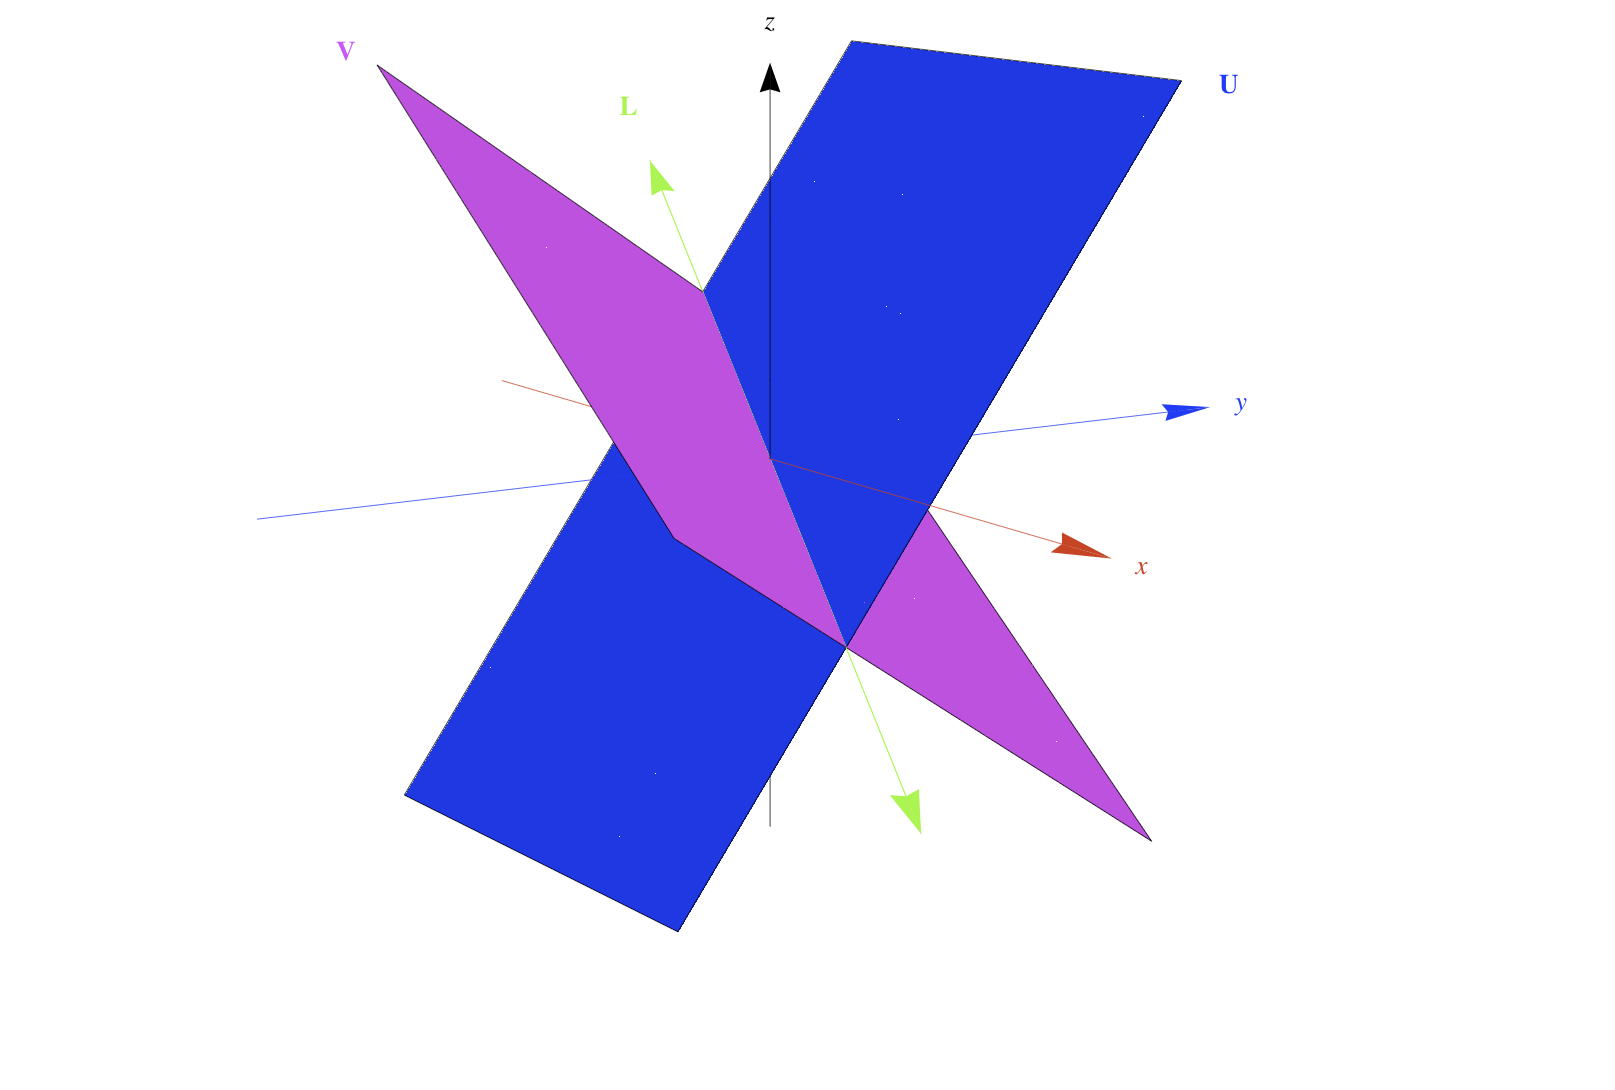
\includegraphics[width=\paperwidth]{img/Planes.jpg}};
\draw (0.5,0.75) node [fill=ocre!30!white,fill opacity=0.6,text opacity=1,inner sep=1cm]{\Huge\centering\bfseries\sffamily\parbox[c][][t]{\paperwidth}{\centering Vector Spaces First\\[15pt] % Book title
{\Large An Introduction to Linear Algebra (Fourth edition)}\\[20pt] % Subtitle
{\small Thierry Giordano, Barry Jessup and Monica Nevins}}}; % Author name
%\draw[thick,red,->,line width=1cm,] (0,0) -- (0.5,0.5) ;
\end{scope}
\end{tikzpicture}

%\newpage
%
%\begin{tikzpicture}[remember picture,overlay]
%\node[inner sep=0pt] (background) at (current page.north) {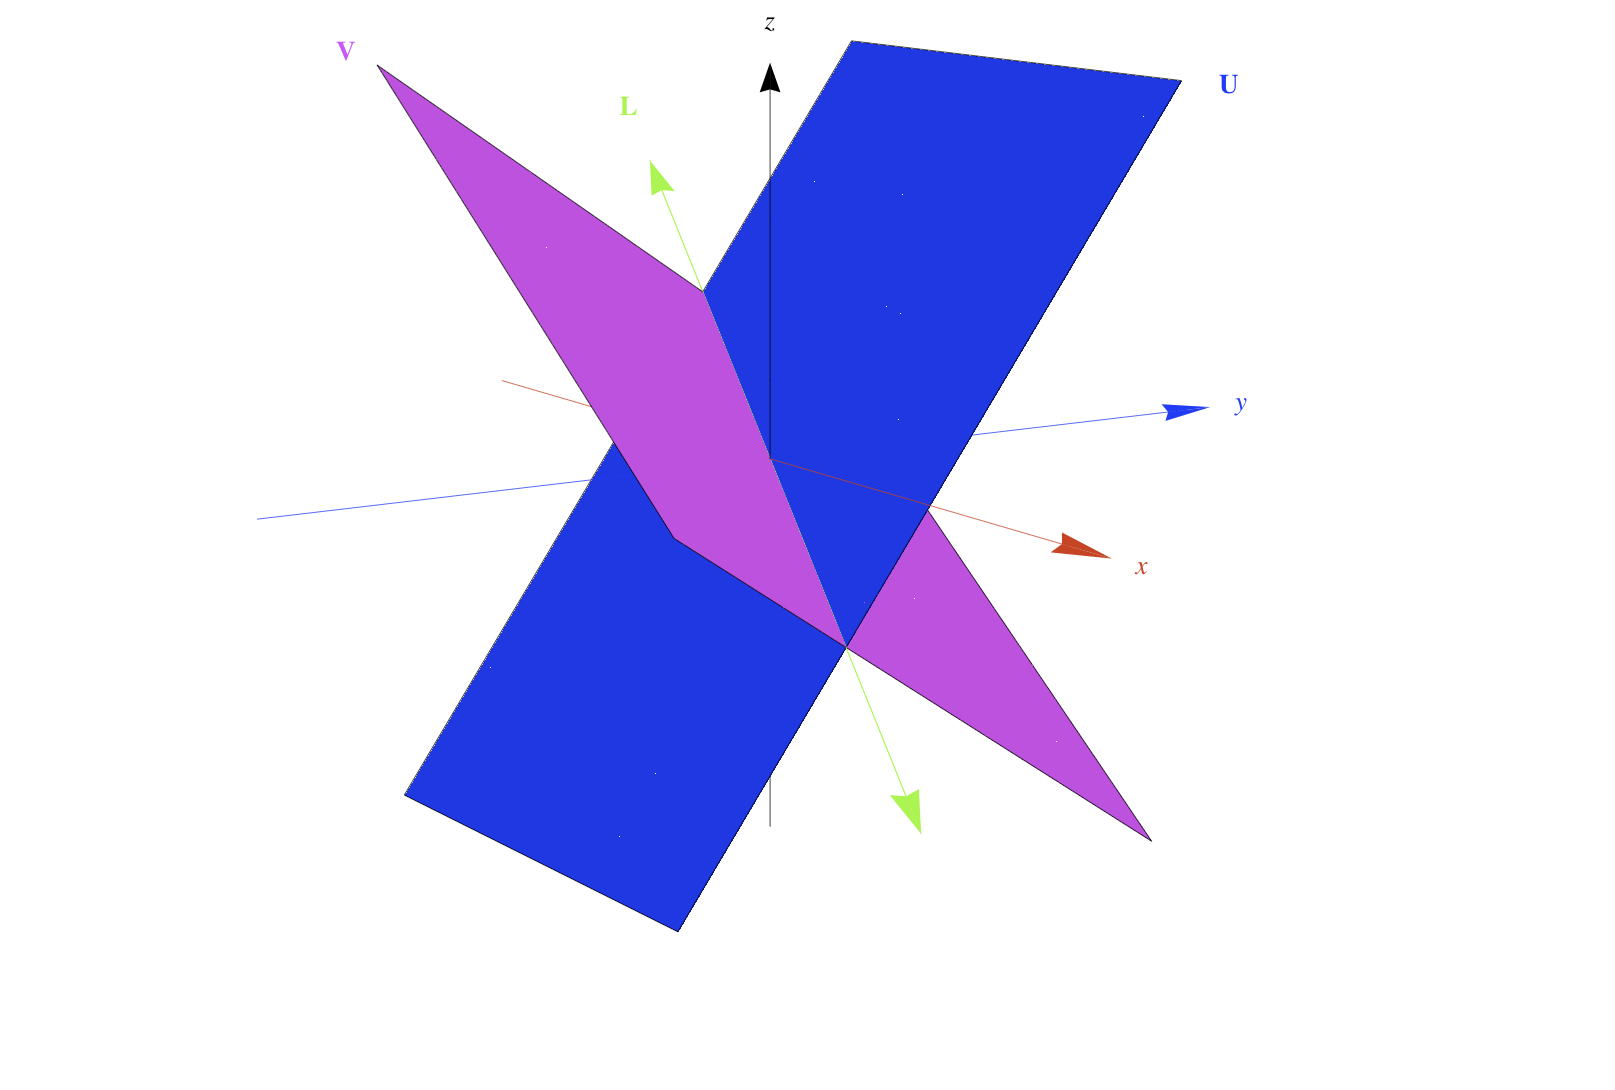
\includegraphics[width=\paperwidth]{img/Planes.jpg}};
%\draw (current page.south) node [fill=ocre!30!white,fill opacity=0.6,text opacity=1,inner sep=1cm]{\Huge\centering\bfseries\sffamily\parbox[c][][t]{\paperwidth}{\centering Vector Spaces First\\[15pt] % Book title
%{\Large An Introduction to Linear Algebra (Fourth edition)}\\[20pt] % Subtitle
%{\small Thierry Giordano, Barry Jessup and Monica Nevins}}}; % Author name
%\end{tikzpicture}
%\vfill
\endgroup

%----------------------------------------------------------------------------------------
%	COPYRIGHT PAGE
%----------------------------------------------------------------------------------------

\newpage
~\vfill
\thispagestyle{empty}

%\noindent Copyright \copyright\ Thierry Giordano, Barry Jessup and Monica Nevins, 2008\\ % Copyright notice




\noindent \copyright\ \textit{Fourth edition, August 2021} % Printing/edition date



\smallskip
\noindent Thierry Giordano, email:
\href{mailto:giordano@uottawa.ca}{giordano@uottawa.ca}



\smallskip
\noindent Barry Jessup, email:
\href{mailto:bjessup@uottawa.ca}{bjessup@uottawa.ca}


\smallskip

\noindent Monica Nevins, email:
\href{mailto:mnevins@uottawa.ca}{mnevins@uottawa.ca}

\smallskip

\noindent \textsc{This document is available at the following locations:} 

\href{https://ruor.uottawa.ca/handle/10393/43430}{https://ruor.uottawa.ca} 

\href{https://github.com/uottawa-mathstat/linear-algebra-oer}{https://github.com/uottawa-mathstat/linear-algebra-oer}  \\% Publisher



\noindent 
\includegraphics{copyright.jpg}

\noindent Unless otherwise indicated, this book is made available under a \href{https://creativecommons.org/licenses/by-nc-sa/4.0/}{Creative Commons Attribution-NonCommercial-ShareAlike 4.0 International licence}.  To view a copy of this license, visit \url{https://creativecommons.org/licenses/by-nc-sa/4.0/}.

\noindent The photographs used in the chapter headings are reproduced with permission from the artist, Ralph Nevins, \url{ralph.ca}, \href{mailto:ralph@nevins.ca}{ralph@nevins.ca}.

\vspace{1in}

%----------------------------------------------------------------------------------------
%	PREFACE
%----------------------------------------------------------------------------------------

%\usechapterimagefalse % If you don't want to include a chapter image, use this to toggle images off - it can be enabled later with \usechapterimagetrue

\chapterimage{Ottawa3.jpg}
% heading image

%%%%%%%%%%%%%%%%%%%%%%preface.tex%%%%%%%%%%%%%%%%%%%%%%%%%%%%%%%%%%%%%%%%%
% sample preface
%
% Use this file as a template for your own input.
%
%%%%%%%%%%%%%%%%%%%%%%%% Springer %%%%%%%%%%%%%%%%%%%%%%%%%% 

\preface
\addcontentsline{toc}{chapter}{Preface}

This volume grew from sets of lecture notes by Thierry Giordano, Barry Jessup,  and Monica Nevins for teaching the course \emph{Introduction to Linear Algebra} at the University of Ottawa.  This book is intended to serve as a text or companion to the course.


The approach we take in this book is not standard: we introduce vector spaces very early and only treat linear systems after a thorough introduction to  vector spaces. 

We do this for at least two reasons. Our experience in teaching variations of this course over the past 25 years  to thousands of students has taught us that the material on vector spaces, usually found toward the end of the course in a traditional textbook, is generally experienced by students as the most difficult part of the course. In a 12 week course, to have the most difficult material near the end of the course does not give most students enough opportunity to come to grips with the (seemingly) new ideas introduced when we meet vector spaces for the first time. 

In our experience, starting with  vector spaces within the first two weeks allows students much more time to appropriate the `big' ideas in linear algebra: the notions of the {\it set of all linear combinations of vectors} (the `span') and the {\it `linear independence' of vectors}. These notions lie at the heart of linear algebra and are usually experienced as new and challenging by students who see them for the first time. So, the sooner they see them, the better: we can use them, as well as the notions of {\it basis} and {\it dimension} in the rest of the course, in different contexts. In this way, it has been our experience that most students prefer to see the challenging material as early as possible, so that they have time to acquaint themselves with material that is genuinely new and different from what they've seen in high school.

Another reason to tackle vector spaces as soon as possible is to alert students to the fact that there {\it is} genuinely new and different material in the course! If one begins with material on linear systems many students have seen in high school, (in low dimensions, at least),  some can easily fall prey to the idea that there's not much to this course, will and will be at caught later on when vector spaces come along.
 



%----------------------------------------------------------------------------------------
%	Acknowledgements
%----------------------------------------------------------------------------------------

\chapterimage{Delta2.jpg}
\chapter*{Acknowledgments -- English Edition}
\addcontentsline{toc}{chapter}{Acknowledgments}

The authors would like to thank those who helped in the making of this book, even though they were completely unaware of it. Our book grew out of our lecture notes for a first year course at the University of Ottawa over a long period, during which time we were guided by  several well-known, excellent and comprehensive texts by authors including Howard Anton, W. Keith Nicholson, David C. Lay, and Seymour Lipschutz and Marc Lipson. Over the years, we also consulted texts by Tom M. Apostol, Otto Brestcher, and Gilbert Strang.



We readily extend our gratitude to colleagues who found the inevitable errors and typos in the first edition. Principally, we thank Anne Broadbent, Saeid Molladavoudi, and Charles Starling who sent us embarassingly long lists of typos and errors as well as many excellent suggestions for changes. 

The book was first used as a text here in the Fall of 2015, and we offer our thanks to the dozens of students in MAT1341 who read our book, found our mistakes and were kind enough to let us know.

That being said, those errors or typos that remain are entirely due to the authors!



\vspace{1in}

{\flushright

Thierry Giordano, Barry Jessup \& Monica Nevins 



January 2015




University of Ottawa

}






%----------------------------------------------------------------------------------------
%	TABLE OF CONTENTS
%----------------------------------------------------------------------------------------

\chapterimage{Rockies.jpg}

\pagestyle{empty} % Disable headers and footers for the following pages

\tableofcontents % Print the table of contents itself

\cleardoublepage % Forces the first chapter to start on an odd page so it's on the right side of the book

\pagestyle{fancy} % Enable headers and footers again

%----------------------------------------------------------------------------------------
%	List of acronyms
%----------------------------------------------------------------------------------------

\chapterimage{Ottawa4.jpg}

%%%%%%%%%%%%%%%%%%%%%%acronym.tex%%%%%%%%%%%%%%%%%%%%%%%%%%%%%%%%%%%%%%%%%
% sample list of acronyms
%
% Use this file as a template for your own input.
%
%%%%%%%%%%%%%%%%%%%%%%%% Springer %%%%%%%%%%%%%%%%%%%%%%%%%%

\chapter*{Acronyms}
\addcontentsline{toc}{chapter}{Acronyms}
\index{acronyms, list of} \index{symbols, list of} 

\paragraph{Common abbreviations used in the text}


\begin{tabular}{ll}
$\col(A)$ &{Column space of the matrix $A$}\\
$\det(A)$ &  {Determinant of the matrix $A$}\\
$\im$ & {Image (of a matrix or linear transformation)}\\
$\ker$ &  {Kernel (of a matrix or linear transformation)}\\
LD & {Linearly Dependent}\\
LI & {Linearly Independent}\\
$\Null(A)$ & {Nullspace of a matrix $A$} \\
REF & {Row Echelon-Form (of a matrix)}\\
$\row(A)$ & {Row space of the matrix $A$}\\
RREF & {Reduced Row Echelon Form (of a matrix)}\\
$\tr(A)$ & {trace of the matrix $A$}
\end{tabular}

%\begin{description}
%\item[Col(A)] {Column space of the matrix $A$}
%\item[$\det$] {Determinant}
%\item[im] {Image (of a linear transformation)}
%\item[ker] {Kernel (of a matrix or linear transformation)}
%\item[LD] {Linearly Dependent}
%\item[LI] {Linearly Independent}
%\item[Null(A)] {Nullspace of a matrix $A$}
%\item[REF]{Row Echelon-Form (of a matrix)}
%\item[Row(A)] {Row space of the matrix $A$}
%\item[RREF]{Reduced Row Echelon Form (of a matrix)}
%\item[tr] {trace (of a matrix)}
%\end{description}

\paragraph{Common symbols}

\begin{tabular}{ll}
$V$ & {a vector space}\\
$U$ & {a subspace of $V$}\\
$\vv$& {a vector}\\
$\zero$&{the zero vector}\\
$A^T$& {transpose of the matrix $A$}\\
$A^{-1}$&{inverse of the matrix $A$}
\end{tabular}

%\begin{description}
%\item[$V$] {a vector space}
%\item[$U$] {a subspace of $V$}
%\item[$\vec{v}$] {a vector}
%\item[$\vec{0}$] {the zero vector}
%\item[$A^T$] {transpose of the matrix $A$}
%\item[$A^{-1}$] {inverse of the matrix $A$}
%\end{description}




%----------------------------------------------------------------------------------------
%	PART I : Algebra and Geometry
%----------------------------------------------------------------------------------------
\chapterimage{Ottawa1.jpg} % Table of contents heading image
%Ottawa1933

\renewcommand{\partintrotext}{A major theme of linear algebra is how to generalize ideas in geometry to
higher dimensions, by interpreting geometric ideas algebraically.  At the same time, one finds that thinking about an algebraic problem geometrically gives
insights into the algebra.

\medskip

We begin our exploration of these themes with a study of the complex numbers, and then a review of some high school geometry (with an eye to extending some of ideas there to higher dimensions).}

\part{Algebra and Geometry}
%%%%%%%%%%%%%%%%%%%%%%part.tex%%%%%%%%%%%%%%%%%%%%%%%%%%%%%%%%%%
% 
% sample part title
%
% Use this file as a template for your own input.
%
%%%%%%%%%%%%%%%%%%%%%%%% Springer %%%%%%%%%%%%%%%%%%%%%%%%%%

\begin{partbacktext}
\part{Algebra and Geometry}
\noindent  
A major theme of linear algebra is how to generalize ideas in geometry to 
higher dimensions, by interpreting geometric ideas algebraically.  At the same time, one finds that thinking about an algebraic problem geometrically gives
insights into the algebra.  

We begin our exploration of these themes with a study of the complex numbers, and then a review of some high school geometry (with an eye to extending some of ideas there to higher dimensions).

\end{partbacktext}





\chapter{Complex Numbers}
\label{Chapter:01complex}


 
In brief, one might say that algebra is the study of solutions of polynomial equations.
Linear algebra is then the study of solutions to linear equations.  (It
gets interesting when you allow multiple variables and multiple equations,
but we'll get to that later.)

For today, let's look at an application of Algebra, as a ``welcome back to
algebra'' for everyone after a long summer away, and as a heads up to
our Engineers (particularly Electrical Engineers) and Physicists 
who will soon be using
complex numbers all the time.



\section{Defining the Complex Numbers}

The history of the complex numbers is very interesting: it does not begin, as one might think, with the equation
$$
x^2 + 1 = 0,
$$ but rather with cubic equations!
Everyone was certain that $
x^2 + 1 = 0
$ has no solutions --  just look at the graph of $y=x^2+1$, they'd argue.\footnote{Indeed, in ancient times one would have said that
$x+1=0$ has no solutions either, since negative numbers don't
represent quantities.} However every \emph{cubic} equation (with real coefficients) does indeed have at least  one real solution - and imaginary numbers (they were called `impossible' numbers for some time) were invented to obtain formulae for the real roots of cubics.\footnote{Search the web for ``the history of complex numbers".} 

 
Nevertheless, let us denote one solution of $
x^2 + 1 = 0
$ by $i$, for ``imaginary'' (notation thanks to Euler, 1777):
$$
i^2 = -1 \qquad \text{or} \qquad i = \sqrt{-1}.
$$
Now we define for a \emph{negative} real number $a$, 
$$\sqrt{a}:=(\sqrt{\vert a\vert}) i.$$

This may seem a bit fussy, but if we simply try to apply the normal rules of algebra, such as in: 
$$
\sqrt{-9} = \sqrt{9 \cdot (-1)} = \sqrt{9} \cdot \sqrt{-1} = 3i,
$$  we obtain the correct answer, but much caution is needed at the third equality.\footnote{A real course in Complex Analysis is needed here, otherwise one can get into trouble: e.g. $9=\sqrt{81}=\sqrt{(-9)(-9)}\not=\sqrt{ -9 }\ \sqrt{ -9 }=3i\, 3i =-9$. Indeed,  the rule for positive real numbers $a,b$ that (correctly) states: $\sqrt{ab}=\sqrt{a}\sqrt{b}$ \emph{does not hold} in general. This may seem like a nuisance but is actually the source of lots of interesting math: search the web for ``Riemann surfaces and the square root".} Stick with the fussy definition for now!
 
(Please note that here, as in Calculus, we adhere to the convention
that for \emph{real} $a$, $\sqrt{a^2} =\vert a \vert$, that is, the answer is the one
positive square root, and not a choice of them.)


  


Now $i$ alone is not quite enough.  Consider the equation
$$
x^2 + 4x + 8 = 0.
$$
By the quadratic formula, its roots are the two numbers
$$
x = \frac{-4 \pm \sqrt{16-32}}{2} = -2 \pm \frac12 \sqrt{-16} = -2 \pm \frac12 (4i) = -2 \pm 2i.
$$
Let's check that this makes sense:  Plug $x = (-2+2i)$ into the 
quadratic equation and simplify:
$$
(-2+2i)^2 + 4(-2+2i) + 8 = (4 -4i - 4i + 4i^2) + (-8 +8i) +8 = 4+4i^2 = 0 
$$
where in the last step we remembered that $i^2 = -1$.  Similarly we
can check that $-2-2i$ is also a root.  




With these thoughts (and the quadratic formula) 
in mind, we make the following definition.

\begin{definition}
The set of \emph{complex numbers} is the set 
$$
\mathbb{C} = \{ a+b\,i \colon a, b \in \mathbb{R} \}.
$$
(Read this as:  ``the set of all things of the form $a+bi$ where $a$ and
$b$ are real numbers''.)

When we write 
$$
z =a +b\,i \in \C
$$
(read as:  $z$ (or $a+b\,i$) belongs to $\C$), then
$a$ is called the \emph{real part} of $z$ (denoted $Re(z)$) and $b$ is called
the imaginary part of $z$ (denoted $Im(z)$).  Note that $Re(z)$ and $Im(z)$
are real numbers!

When $Re(z)=0$ then $z=bi$ and we say $z$ is \emph{purely imaginary};
when $Im(z)=0$ then $z=a$ is real.  Thus $\R \subset \C$ (read as:  $\R$
is a subset of $\C$).
\end{definition}

The real numbers were drawn as the real number line; the complex numbers
are drawn as the complex \emph{plane} as we shall soon see.  

 So notice that given any quadratic equation $ax^2+bx+c=0$, with real coefficients $a,b,c$, the roots are $$x = \frac{-b}{2a} \pm \frac{\sqrt{b^2-4ac}}{2a}. $$ If $b^2-4ac \geq 0$, the roots are real, otherwise, they are complex numbers.  So now EVERY quadratic equation has two roots (counting a double root as two, now and always). 

\section{Algebra of the Complex Numbers}

\begin{itemize}
\item Equality:  $a+bi = c+di \Leftrightarrow \textrm{$a=c$ and $b=d$}$;
\item Addition:  $(a+bi) + (c+di) = (a+c) + (b+d)i$
\item Multiplication:  $(a+bi)(c+di) = (ac-bd) + (ad+bc)i$
\end{itemize}
In fact, complex numbers satisfy all the same properties as
$\R$ except there is no ordering (that is, ``$z>y$'' doesn't 
make sense).  

What about division?

\begin{myprob}
Solve $(4+3i)z = 1$, if possible; that is, what do we mean by
$$
z = \frac{1}{4+3i} ?
$$
(PLEASE PLEASE remember that $\frac{1}{2+3} \neq \frac12 + \frac13$!!!!)


\begin{mysol}
The idea:  remember that $i$ is a square root -- so  use the  standard trick of algebra called \emph{rationalizing the denominator}.

So 
 $$(a+b \, i)(a-b\, i) = a^2-(b\, i)^2 = a^2+b^2$$ As   $a$ and $b$ are \emph{real}, $a^2+ b^2 \neq 0$,
unless both $a$ and $b$ are zero.
So for $z=a+bi$, let 
\begin{itemize}
\item $\overline{z} = a-bi$, the complex conjugate of $z$
\item $\vert z \vert = \sqrt{a^2+b^2}$, the absolute value, or modulus, of $z$
\end{itemize}
(Note:  $z = 0$ if and only if (iff) $\vert z \vert = 0$; and we CAN
compare moduli of complex numbers:  $\vert i \vert = \vert 1 \vert > \vert 0 \vert$.  Also note that we used complex conjugates in the quadratic formula;
this is familiar!)

Now we have
$$
z \overline{z} = \vert z \vert^2
$$
so
$$
z \cdot \left(\frac{\overline{z}}{\vert z \vert^2}\right) = 1
$$
or
$$
\frac{1}{z} = \frac{\overline{z}}{\vert z \vert^2}.
$$
Excellent!  So 
$$
\frac{1}{4+3i} = \left(\frac{1}{4+3i} \right) \left( \frac{4-3i}{4-3i} \right) = \frac{4-3i}{4^2+3^2} = \frac{4-3i}{25} = \frac{4}{25} - \frac{3}{25}i.
$$
\end{mysol}\end{myprob}

 
\begin{myprob}
Simplify
$$
\frac{3+2i}{-2+4i}
$$

\begin{mysol}
Multiply by $1 = \frac{-2-4i}{-2-4i}$:
$$
\frac{3+2i}{-2 + 4i} = \frac{3+2i}{-2 + 4i}\cdot \frac{-2-4i}{-2-4i} =
\frac{(3+2i)(-2-4i)}{4+8i-8i-16i^2} = \frac{2-16i}{20} = \frac{1}{10} - \frac{4}{5}i.
$$
This is what we wanted:  the answer is in a form that we recognize as 
a complex number.
\end{mysol}
\end{myprob}

Some other properties (easy to prove):

\begin{lemma}[Properties of Complex Numbers] 
Complex conjugation has the following properties.  Suppose that
$z,w \in \C$ and $c\in \R$.  
\begin{itemize}
\item $\displaystyle \frac{1}{z} = \frac{\overline{z}}{\vert z \vert^2}$\smallskip
\item $\overline{z+w} = \overline{z} + \overline{w}$.
\item $\overline{cz} = c\overline{z}$.
\item $\overline{zw} =\overline{z}\; \overline{w}$.
\item $\overline{z/w} = \overline{z}/\overline{w}$.\smallskip
\item $\overline{\overline{z}} = z$ (eg:  $\overline{\overline{3+2i}}= \overline{3-2i} = 3+2i$)
\item $\overline{z} = z$ iff $z \in \R$
\item $\overline{z} = -z$ iff $z$ is purely imaginary


\item $\vert z \vert \in \R$ and $\vert z \vert \geq 0$
\item $\vert z \vert = \vert \overline{z} \vert$
\item $\vert zw \vert = \vert z \vert \; \vert w \vert$
\item $\vert z/w \vert = \vert z \vert / \vert w \vert$
\item $\vert z + w \vert \leq \vert z \vert + \vert w \vert$ (`Triangle inequality')
\item If $a$ is a real number then $\vert a + 0i \vert$ is the 
absolute value of $a$.  (So we just write $z=a$ rather than
$z=a+0i$; there's no problem.)


\end{itemize}
Essentially what this is saying is that in any expression for a complex number $z$, the expression for
$\overline{z}$ is given by replacing each occurence of the symbol ``$i$''
with ``$-i$''; you don't have to simplify it first.
\end{lemma}

\begin{proof}
(You can discuss these with me, or with the TA in the DGD.
Proving such things is important because it shows you WHY 
something is true, and that in turn makes it hard to forget, 
or remember falsely.)

(2) Suppose $z$ and $w$ are complex numbers.  
That means
$z = a+bi$ for some real numbers $a$ and $b$, and $w = c+di$
for some real numbers $c$ and $d$.
Then $$z+w = (a+c) + (b+d)i \qquad \text{so} \qquad \overline{z+w} = (a+c) - (b+d)i.$$
On the other hand, $\overline{z} = a-bi$ and $\overline{w} = c-di$,
so that $$\overline{z} + \overline{w} = (a+c)+(-b-d)i = (a+c)-(b+d)i.$$
Hence the two sides are equal, which completes the proof.

We prove another one,  and leave the rest as exercises.  
(For the triangle inequality, it's easier to use geometry, below;
and for the multiplicative property, it's easier to use
polar form.)

(10) Suppose $z$ is a complex number.  Then 
$$
\vert z \vert = \sqrt{z \overline{z}}
$$ 
whereas 
$$
\vert \overline{z} \vert = \sqrt{\overline{z} \ \overline{\overline{z}}}  = \sqrt{\overline{z} z }= \sqrt{ z \overline{z} }= \vert z \vert
$$ 
by all that we've established before.  So the two are equal.
\end{proof}


\section{Geometry of the complex numbers}  

\begin{center}
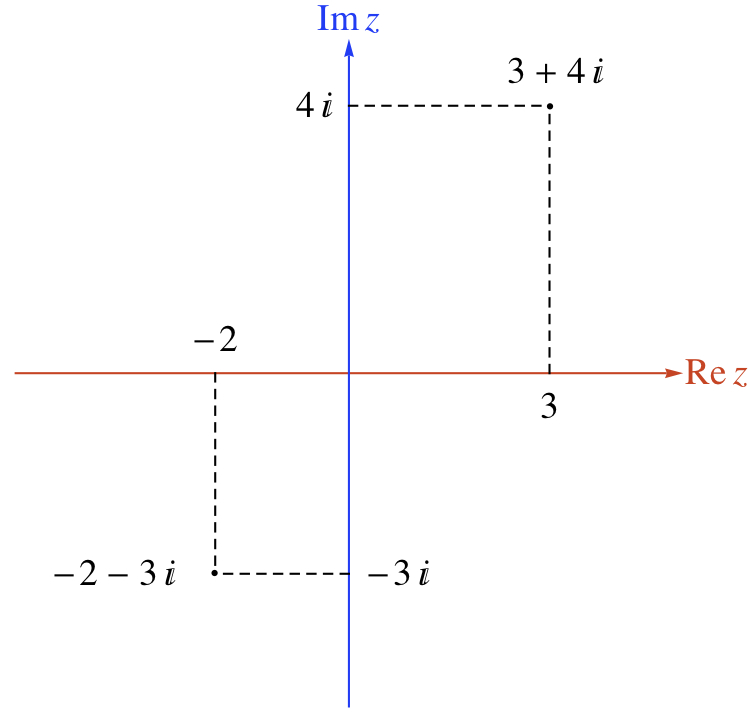
\includegraphics[scale=.6]{img/complexplane.jpg}
\end{center}
Each complex number
is written as $a+b\,i$ with $a$ and $b$ real numbers.  To picture
this, think of $a+b\,i$ as the point $(a,b)$ in the $xy$-plane.
Then $a+b\,i$ is a point in the plane, which in this context
we call the \emph{complex plane}.  The horizontal axis is called
the \emph{real axis} and the vertical axis 
is called the \emph{imaginary axis}.

Addition of two complex numbers is the same as the addition of
two vectors in the plane.  The negation of a complex number is
just the negation of the corresponding vector.  Multiplication
by real numbers is just scalar multiplication, but multiplication
by complex numbers is a combination of rotation and scaling
(try it out!).

Complex conjugation is just the reflection of the vector through the real
axis.  So if $z = a+b\,i$ then $\overline{z} = a-b\,i$.  

The modulus of $z$ is just the length of the vector representing $z$.
(Recall that the length of the vector from the origin to $(a,b)$ is
$\sqrt{a^2+b^2}$. )

\section{Polar Form of Complex Numbers} 



These are also called ``polar coordinates'' and show up in 
Calculus II, for the real plane.  


 \begin{center}
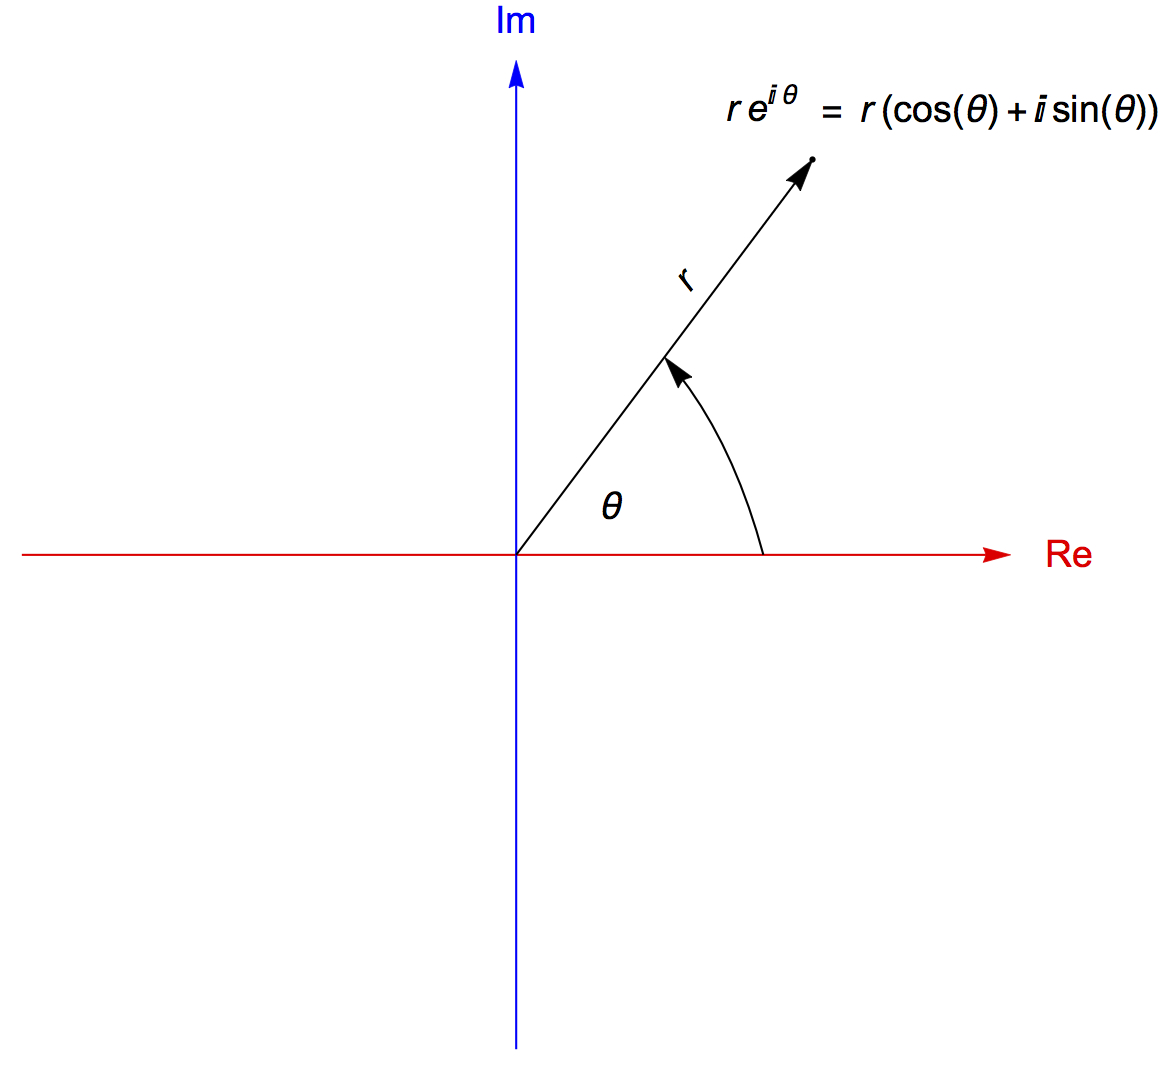
\includegraphics[scale=.5]{img/PolarForm.jpg}
\end{center}




So if $z = x+y\,i \in \C$ then 
$$
\frac{x}{r} = \cos(\theta), \quad \frac{y}{r} = \sin(\theta)
$$
and
$$
r = \vert z \vert = \sqrt{x^2+y^2}
$$
Therefore:  
$$
z = x+yi = r \cos(\theta) + i r\sin(\theta) = r(\cos(\theta)+i \sin(\theta)).
$$
(Note that $\theta = \arg(z)$ (argument of $z$) is not uniquely determined,
since $\theta' = \theta + 2n\pi$, $n\in \Z$, also works.  We usually
pick $-\pi < \theta \leq \pi$ and write $\theta = \Arg(z)$, the principal
argument of $z$.)

In 1748, Euler proved
$$
e^z = 1 + z + \frac{z^2}{2} + \cdots = \sum_{n=0}^\infty \frac{z^n}{n!}
$$
(power series) so in fact by comparing power series with trig functions
we get, surprisingly,
$$
e^{i\theta} = \cos(\theta) + i\sin(\theta).
$$ 
So modern notation is:  the \emph{polar form} of the complex number $z$
is 
$$
z = r e^{i\theta}.
$$

\begin{example}
See the diagram below and check that  $2i= 2e^{i \frac{\pi}2}$, $-i=e^{-i \frac{\pi}2}$, $-1 = e^{i\pi}$, and  
$1+i =\sqrt{2}e^{i \frac{\pi}4}$
\end{example}
\begin{center}
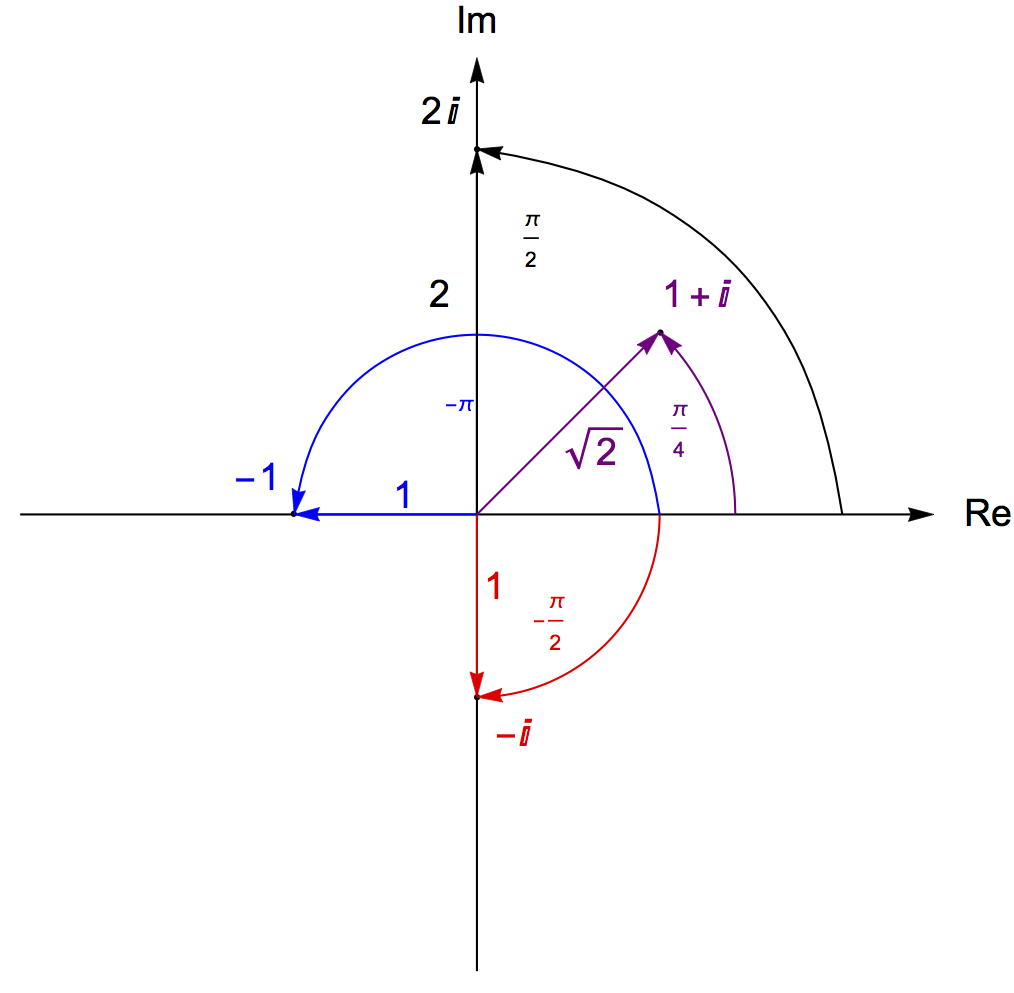
\includegraphics[scale=.6]{img/PolarFormExample.jpg}
\end{center}


We have
\begin{itemize}
\item  $re^{i\theta} = r' e^{i\theta'}$ iff $r=r'$ and $\theta = \theta' + 2n\pi$, some $n\in Z$.
\item $\overline{re^{i\theta}} = re^{-i\theta}$
\item $\vert e^{i\theta} \vert = 1$ for any $\theta$
\end{itemize}

\section{Multiplying complex numbers in polar form}

Note that if $z = re^{i\theta}$ and $w = se^{i\phi}$ then
\begin{align*}
zw &= \left( r(\cos(\theta)+i\sin(\theta)) \right) \left(s (\cos(\phi)+i\sin(\phi)\right) \\
&= (rs)\left( (\cos(\theta)\cos(\phi) - \sin(\theta)\sin(\phi)) + i(\cos(\theta)\sin(\phi) + \sin(\theta)\cos(\phi)) \right)\\
&= rs(\cos(\theta + \phi) + i\sin(\theta + \phi))\\
&= rse^{i(\theta+\phi)}
\end{align*}
That is:  it's like the usual multiplication with exponents.  (Same for
division.)
 
\begin{myprob}
Compute
$$
\frac{i}{1+i}
$$

\begin{mysol}
From before, we have $i = e^{i\frac{\pi}{2}}$ and 
$1+i = \sqrt{2}e^{i\frac{\pi}{4}}$
so
$$
\frac{i}{1+i} = \frac{e^{i\frac{\pi}{2}}}{\sqrt{2}e^{i\frac{\pi}{4}}}
 = \frac{1}{\sqrt{2}}e^{i\frac{\pi}{4}}
$$
(check, using the long method!)

\end{mysol}
\end{myprob}

\section{The Fundamental Theorem of Algebra}



We noted above that every quadratic polynomial with real
coefficients has two roots, and in fact if one root was
complex and not real, then so was the other, and the two
roots are complex conjugates.

Conversely, given a complex number $z$, one polynomial
with roots $z$ and $\overline{z}$ is 
$$
(x-z)(x-\overline{z}) = x^2 -(z+\overline{z})x + z \overline{z}.
$$
Is this a polynomial with real coefficients?  YES!  Write
$z = a+ib$, then $z+\overline{z} = 2a$, which is real; and
$z \overline{z}$ is real (as we proved earlier).  

So:  every real polynomial has complex roots, and every
complex number is the root of some real polynomial.  

That said, if you take two complex numbers $z$ and $w$ which
are not conjugate, then $(x-z)(x-w)$ will just be some
random quadratic polynomial with complex coefficients.
Which begs the question:  if you take all quadratic polynomials
with complex coefficients, and use the quadratic formula to
solve them, what extra numbers (like $i$) do you need this 
time?  

Answer:  NONE.  The complex numbers are the top of the heap,
and all you'll ever need:

\begin{theorem}[Fundamental Theorem of Algebra]
Every polynomial with coefficients in the complex numbers
factors completely into linear factors of the form $ax+b$,
with $a,b \in \mathbb{C}$.
\end{theorem}

\section[Some musings about the Fundamental Theorem of Algebra]{Some musings about the meaning of the Fundamental
Theorem of Algebra}

 This answers a really big nagging problem
of algebra: shouldn't every quadratic have 2 roots, and 
every cubic 3 (allowing multiple roots)?  But the quadratic
$x^2+2$ didn't have any roots over the reals.  

In Calculus,
we accept this by sketching the graph of $y=x^2+2$ and saying,
``Look, it doesn't intersect the $x$-axis.  That explains it.''

``Explains what, exactly?'' an algebraist responds.  ``You're 
still missing two roots.''  

In algebra, we are looking for unifying themes, things that
are common across all problems of a particular type.  We look
for wonderful universal solutions.  The complex numbers are
one example of a universal solution:  we added $\sqrt{-1}$
and suddenly all problems were solved:  $x^2+2$ has two roots,
and $ix^7+3x^2-(4+i)$ has 7 roots.  

(Well, one might admit, not all problems are completely solved.
The Fundamental Theorem of Algebra doesn't say ANYTHING about
FINDING the roots.  It just says that they exist.  We end up
going back to Calculus for help in finding them.)

For the rest of this course, we will be considering LINEAR algebra,
which is a particular branch of algebra where, it turns out, there
are fantastically universal solutions to absolutely everything
(not just ``existence'', but actually ways of finding solutions!).


%
% Use the following environment.
% Don't forget to label each problem;
% the label is needed for the solutions' environment

\section*{Problems}
\addcontentsline{toc}{section}{Problems}
Those marked with a $\star$ have solutions at the back of the book. Try them yourself first.

\begin{prob}
\label{prob01.1}\sov

 Express the following complex numbers in  Cartesian form: $a + b \,i$, with $a, b \in \R$.
\medskip
\begin{enumerate}[a)]
\item    $(2+i)(2+2 i)$ \medskip  
\item $ \dfrac 1{1+i}$\medskip 
\item $  \dfrac{8+3i}{5-3i}$\medskip 
\item $\dfrac{5+5\sqrt{3}\,i}{\sqrt{2}-\sqrt{2}\,i}$\medskip 
\item $\dfrac{(1+2i)(2+5i)}{3+4i}$\medskip  
%$\dfrac{ 12}{25} +\dfrac{59}{25}i  $

\item $\dfrac{1-i}{2-i}+\dfrac{2+i}{1-i}$\smallskip
% 
\item $\dfrac 1{(1-i)(3-2i)}$
%
\end{enumerate}

\end{prob}
\begin{prob}
\label{prob01.2}\sov  Find the polar form of the following complex numbers: (i.e., either  as $r e^{i\theta}$ or as $r(\cos \theta + i \sin \theta)$, with $r\geq 0$ and $-\pi <\theta \leq \pi$)\medskip
\begin{enumerate}[a)]

\item ${3\sqrt{3}-3i}$\medskip
%$6(\cos (-\pi /6)+i \sin (-\pi /6)) $
\item $\dfrac{3\sqrt{3}-3i} {\sqrt{2}+i\sqrt{2}}$\medskip
%$3(\cos (-5\pi /12)+i \sin (-5\pi /12)) $

\item $\dfrac{1-\sqrt{3}i}{-1+i}$ \medskip
%$\sqrt{2}(\cos (11\pi/12)+i\sin (11\pi /12))$
\item $\dfrac{5+5\sqrt{3}i}{\sqrt{2}-\sqrt{2}i}$ \medskip
%$5(\cos (7\pi /12)+i\sin (7\pi/12))$
\item $\dfrac{3+3\sqrt{3}i} {-2+2i}$ \medskip
% $\dfrac{3}{\sqrt{2}}(\cos (5\pi /12)-i\sin (5\pi/12))$
\end{enumerate}

\end{prob}
\begin{prob}
\label{prob01.3} Find the modulus of each of the complex numbers in questions 1 \& 2. (Remember that $|z w|=|z|\, |w|$ and that if $w\not=0$, then $\displaystyle\left| \frac{z}{w} \right| = \frac{\left| z\right|}{\left|w\right|}$.) %\Big|\dfrac{z}{w}\Big|=\dfrac{|z|}{|w|}$.)

\end{prob}
\begin{prob}
\label{prob01.4}\sov   If $z$ is a complex number,

(i)  Is it possible that $z={\bar z}$?

(ii)  Is it possible that $|{\bar z}|>|z|$?

(iii)  Is it possible that ${\bar z}=2z$? 

\medskip Give  examples to illustrate your affirmative answers, and explanations if you say the statement is always false.
 \end{prob}






\begin{prob}
\label{prob01.5}
\textbf{For budding algebraists...}\\
Show that there is no `proper' ordering on the complex numbers, that is, there is no binary relation $>$ with the property that if $x>0$ and $y>z$ then $xy>xz$.
 \end{prob}
\chapter{Vector Geometry}
\label{Chapter:02vectors}
 
Much of the material in this chapter may be review from high
school, but it allows us to set the stage 
 for the upcoming chapters.



\section{Vectors in \texorpdfstring{$\R^n$}{Rn}}

\stress{Vector} comes from the Latin \textit{vehere}, which means to carry,
or to convey; abstractly we think of the vector as taking us along the
arrow that we represent it with.  For example, we use vectors in Physics to indicate the magnitude and direction of a
force.

Let's use our understanding of the geometry and algebra of vectors in
low dimensions (2 and 3) to develop some ideas about the geometry and
algebra in higher dimensions.

\begin{center}
\begin{tabular}{ll}
Algebra & Geometry \\
\hline
$\R$, real numbers, \defn{scalars} & real line\\
$\R^2 = \{(x,y) | x,y\in\R\}$, vectors $\uu = (x,y)$ & plane \\
$\R^3 = \{(x,y,z) | x,y,z\in\R\}$, vectors $\uu = (x,y,z)$ & 3-space \\
\vdots & \\
(why not keep going?) & \\
\vdots & \\
$\R^4 = \{(x_1,x_2,x_3,x_4) | x_i \in \R\}$, vectors $\xx = (x_1,x_2,x_3,x_4)$ & \\
Hamilton (1843): extended $\C$ to \defn{hamiltonians} & \defn{space-time}\\
& \\
$n \in \Z$, $n>0$: $\R^n = \{ (x_1, x_2,\cdots,x_n) | x_i \in \R\}$ &\\
$\xx = (x_1, \cdots, x_n)$ & $n$-space
\end{tabular}
\end{center}

\paragraph{Notation}  We have several different notations which we use for
writing vectors, which we use interchangeably:
\begin{itemize}
\item $\xx = (1,2,3,4)$
\item $\xx = \mat{1\\2\\3\\4}$
\item $\xx = \mat{1\;&2\;&3\;&4}^T$, where the exponent T stands for
\defn{tranpose}.  (\emph{Transposition}\index{transposition} means turning rows into columns (and \emph{vice versa}).)
\end{itemize}
The vertical notation (also referred to as \defn{matrix form}) is the easiest to read but the first one is easier
to write.

  

(The reason for the vertical
vector notation comes from matrix multiplication, which we'll get to later.)

\section{Manipulation of vectors in \texorpdfstring{$\R^n$}{Rn}}  

The algebraic rules for $\R^n$ extend directly from the algebraic
rules for $\R^2$ and $\R^3$: 
\begin{itemize}
\item Equality:  $(x_1,\cdots, x_n) = (y_1,\cdots, y_n) \Leftrightarrow x_i=y_i$ for all $i \in \{1,\cdots,n\}$.  (In particular, $(x_1,\cdots,x_n) \neq (y_1,\cdots, y_m)$ if $n \neq m$.)

\item Addition:  $(x_1,\cdots,x_n) + (y_1,\cdots, y_n) = (x_1+y_1, \cdots, x_n+y_n)$
\item Zero vector:  $\zero = (0,0,\cdots, 0) \in \R^n$
\item Negative:  if $\xx = (x_1,\cdots,x_n)$ then $-\xx = (-x_1,\cdots,-x_n)$
\item Multiplication {\bf by a scalar}:  let $c\in \R$ be a scalar, then
$c(x_1,\cdots,x_n) = (cx_1,\cdots,cx_n)$
\end{itemize}
Note that we don't have any way of \stress{multiplying} two vectors; the closest
we can get to that is the \stress{dot product}, which gives a scalar as an 
answer, or the \stress{cross product}, which only works in $\R^3$\footnote{However, there are ways generalize the cross product in $\R^n$ for every $n$, but the product doesn't live in $\R^n$! Search the web for `exterior algebra'.}.
 There's even a way to have `multi-products' of $n-1$ vectors in $\R^n$, and get an answer in $\R^n$. Once you've seen the {\it determinant} later, you'll know exactly what to do if you look again at the definition of the cross product.

There are geometric interpretations of each of the above algebraic
rules, which we can draw in $2$ (and $3$, if you draw well) dimensions.
\begin{itemize}
\item Equality:  two vectors are equal if they have the same magnitude
and direction
\item Addition:  parallelogram rule, or head-to-tail rule 

\item Zero vector:  the vector with zero length
\item Negative: the same arrow with head and tail exchanged
\item Scalar multiple:  scale the vector by $\vert c \vert$, and change
direction if $c<0$; or:  two vectors are \emph{parallel} if and only if 
they are scalar multiples of one another.
\end{itemize}

\section{Linear combinations (Important Concept!)}
The only operations we have are:  vector addition, and scalar multiplication.
We are going to be interested in the question:  If I already have the
vectors $\uu_1$, $\uu_2$, $\cdots$, $\uu_m$ (that is, $m$
vectors in $\R^n$), can I produce another  vector 
by scaling each vector and adding them together, in some way?

By analogy:  Say $\uu_1$ is parallel to Bank Street pointing north 
and $\uu_2$
is parallel to Laurier Ave, pointing east; then I can get anywhere downtown by 
going in the direction of $\uu_1$ (or its negative) 
for a little way, and then taking direction $\uu_2$ (or its
negative) for a little way.  But I can't get underground, or
into the air, by following those directions.  I'm stuck on the
plane which is the ground.

Algebraically, this all comes down to the following definition.

\begin{definition} \index{linear combination}
If $k_1,k_2,\cdots, k_m \in \R$ are scalars, and $\uu_1,\uu_2,\cdots,\uu_m\in \R^n$ are vectors, then 
$$
k_1\uu_1+k_2\uu_2 + \cdots + k_m\uu_m 
$$
is called a \emph{linear combination} of $\uu_1,\uu_2,\cdots,\uu_m$.
\end{definition}

\begin{myexample}
Let $\uu_1 = (1,2,3)$ and $\uu_2 = (1,0,0)$.  

Then $\xx = (17,4,6)$ is a linear combination of $\uu_1$
and $\uu_2$ because
$$
\mat{17\\4\\6} = 2 \mat{1\\2\\3} + 15 \mat{1\\0\\0}.
$$
But $\yy = (0,1,0)$ is \emph{not} a linear combination of
$\uu_1$ and $\uu_2$ because the equation
\begin{equation} \label{E:1}
\mat{0\\1\\0} = a \mat{1\\2\\3} + b\mat{1\\0\\0}
\end{equation}
would imply 
\begin{align*}
\mat{0\\1\\0} &= \mat{a\\2a\\3a} + \mat{b\\0\\0}\\
&= \mat{a+b\\ 2a \\ 3a}
\end{align*}
So that
$$
0 = a+b, \quad  1 = 2a, \quad \text{and} \quad 0 = 3a;
$$ 
but the second and third equations are contradictory, so
there cannot be a solution to \eqref{E:1}.  Thus $\yy$
isn't a linear combination of $\uu_1$ and $\uu_2$.
\end{myexample}

\section{Properties of vector addition and scalar multiplication}



Note that all the usual algebraic properties of addition and
scalar multiplication hold, whether our vectors have $2$
components or $n$ components.  That is, let $\uu,\vv,\ww\in\R^n$
and let $c,c' \in \R$; then we have:
\begin{itemize}
\item $\uu+\zero = \uu$
\item $\uu + (-\uu) = \zero$
\item $(\uu + \vv) + \ww = \uu + (\vv+\ww)$

\item $\uu+\vv = \vv+\uu$
\item $c(\uu+\vv) = c\uu + c\vv$
\item $(c+c')\uu = c\uu + c'\uu$
\item $(cc')\uu = c(c'\uu)$
\item $1 \uu = \uu$
\end{itemize}
Bear these properties in mind, as they are the key to generalizing
to vector spaces beyond $\R^n$.

\section{More geometry: the Dot Product in \texorpdfstring{$\R^n$}{Rn}}  

The \defn{dot product} (also called an \defn{inner product}) gives us
an algebraic way to describe some interesting geometric properties:
length of a vector, and angle between two vectors.

Recall the dot product from $\R^3$:

Let $\uu = (x_1,x_2,x_3)$ and $\vv = (y_1,y_2,y_3)$ be two vectors in
$\R^3$.  Then their dot product is
$$
\uu \cdot \vv = x_1y_1 + x_2y_2 + x_3y_3.
$$
Note that this is a scalar.

Once we have the dot product, we define:
\begin{itemize}
\item $\Vert \uu \Vert = \sqrt{x_1^2+x_2^2+ x_3^2} = \sqrt{\uu \cdot \uu}$, the \emph{length} or \emph{norm} of $\uu$;
\item $\Vert \uu - \vv \Vert$ is the \emph{distance between $\uu$ and $\vv$}.
\end{itemize}
We can see that this is correct, by drawing a cube with main diagonal $\uu$
and noting that the length of the main diagonal is given by the square
root of the sum of the squares of the lengths of the sides by repeated
applications of the Pythagorean theorem.

So, let's generalize this to $\R^n$:

\begin{definition}
Let $\uu = (x_1,\ldots,x_n)$ and $\vv = (y_1,\ldots,y_n)$ be vectors
in $\R^n$.  Then their \defn{dot product} is defined to be 
$$
\uu \cdot \vv = x_1y_1 + \cdots + x_ny_n
$$
and the \defn{norm} of $\uu$ is defined to be
$$
\Vert \uu \Vert = \sqrt{\uu \cdot \uu} = \sqrt{x_1^2+\cdots+x_n^2}
$$
We sometimes call $\R^n$, equipped with the dot product, \defn{Euclidean
$n$-space}.\footnote{As opposed to, for example, 'Minkowski spacetime', where the `lengths' of vectors can be imaginary! Search the web for `minkowski space wiki'.}
\end{definition}


\begin{myexample}
Let $\uu = (1,2,-1,0,1)$, $\vv = (1,3,2,1,1)$.  Then
$$
\uu \cdot \vv = 1+6-2+0+1 = 6
$$
and
$\Vert \vv \Vert = \sqrt{1+9+4+1+1} = \sqrt{16}=4$.
\end{myexample}

Note that for any vector $\uu \in \R^n$:
$$
\Vert \uu \Vert = 0 \Leftrightarrow \uu = \zero
$$
(because the norm is still the sum of real squares, and so
is never zero unless each component is).

\section{Orthogonality}

Recall that in $\R^2$ and $\R^3$, we have that
$$
\uu \cdot \vv = 0 \Leftrightarrow \textrm{$\uu$ and $\vv$ are orthogonal ( or `perpendicular').}
$$

\begin{definition}
Let $\uu,\vv \in \R^n$.  Then $\uu$ and $\vv$ are said to be
\defn{orthogonal} if $\uu \cdot \vv = 0$.
\end{definition}

\begin{myexample}
The vectors $(1,2,-2,1)$ and $(4,1,3,0)$ of $\R^4$ are orthogonal
(perpendicular), since
$$
\mat{1\\2\\-2\\1} \cdot \mat{4\\1\\3\\0} = 4+2-6+0 = 0.
$$
\vglue -.5cm
\end{myexample}

\section{Angles between vectors in \texorpdfstring{$\R^n$}{Rn}}

Now saying that two vectors are orthogonal is another way of
saying that they meet at a $90^\circ$ angle.  We can determine
the angle between vectors in $\R^2$ and $\R^3$; can that be
generalized as well?  We need to know one fact:


\begin{theorem}[Cauchy-Schwarz Inequality]
If $\uu,\vv \in \R^n$, then 
$$
\vert \uu \cdot \vv \vert \leq \Vert \uu \Vert \; \Vert \vv \Vert
$$
\end{theorem}

The proof\footnote{For $x\in\R$, consider the   quadratic function $q(x)=\|u+ x v\|^2$. Expand the right hand side as $(u+ x v)\cdot (u+ x v)$, compute the discriminant `$b^2-4ac$', which (as $q(x)\ge 0$ for all $x$) must satisfy $b^2-4ac\le 0$. Simplifying this, one obtains the desired inequality.} is straightforward.

Applying this to $\Vert \uu + \vv \Vert^2 = (\uu + \vv)\cdot(\uu+\vv)$
yields
$$
\Vert \uu + \vv \Vert \leq \Vert \uu \Vert + \Vert \vv \Vert
$$
which is the \defn{triangle inequality} (which looks the same as the one we noted for $\C$
in our first class).

\begin{definition}
If $\uu,\vv \in \R^n$ and $\uu,\vv \neq \zero$, then the angle
$\theta$ between $\uu$ and $\vv$ is defined to be the number
$\theta$ which satisfies:
\begin{itemize}
\item $\displaystyle \cos \theta = \frac{\uu \cdot \vv}{\Vert \uu \Vert\; \Vert \vv \Vert}$
\item $0 \leq \theta \leq \pi$
\end{itemize}
(The first condition makes sense because
of the Cauchy-Schwarz inequality, since this inequality implies that the number on the right hand
side is always between $-1$ and $1$. The second condition guarantees uniqueness of $\theta$. )
\end{definition}

\begin{myexample}
The angle between $\uu = (0,0,3,4,5)$ and $\vv = (-1,1,-1,1,2)$
is $\theta$, where
$$
\cos(\theta) = \frac{\uu \cdot \vv}{\Vert \uu \Vert\; \Vert \vv \Vert}
= \frac{11}{\sqrt{50}\sqrt{8}} = \frac{11}{20}.
$$
 We find $\theta = \arccos(11/20)$.\footnote{With the help of a calculator --which you'll never need in this course --, $\theta \simeq 0.988432\simeq56.6^\circ$.}
\end{myexample}

Of particular interest:
\begin{itemize}
\item Two non-zero vectors $\uu$, $\vv$ are orthogonal if the angle between
them is $\frac{\pi}2$ (or $90^\circ$).  Now $\cos(\frac{\pi}2) = 0$, so by our formula,
the numerator $\uu \cdot \vv$ has to be zero.  That's where the
orthogonality condition came from.
\item Two vectors $\uu$ and $\vv$ are parallel if the angle between
them is either $0^\circ$ or $\pi$.  Now $\cos(0) = 1$ and
$\cos(\pi) = -1$, so in this case $\uu \cdot \vv = \pm \Vert \uu \Vert\; \Vert \vv \Vert$ attains its maximum value (in absolute terms).
\end{itemize}

\section{Orthogonal Projections onto lines in \texorpdfstring{$\R^n$}{Rn}}
 
The idea of the 
orthogonal projection is:  given two nonzero vectors $\uu$ and $\vv$,
then the \defn{projection of $\vv$ onto $\uu$}, denoted

  
$$
 \proj_{\uu}(\vv)
$$ 
is the unique vector which satisfies
\begin{itemize}\label{propOrthogProj}
\item $\proj_{\uu}(\vv)$ is parallel to  
$\uu$ (so a scalar multiple of $\uu$)
\item $\vv - \proj_{\uu}(\vv)$ is orthogonal to $\uu$ (so gives dot product zero).
\end{itemize}
 
\begin{figure}
\begin{center}
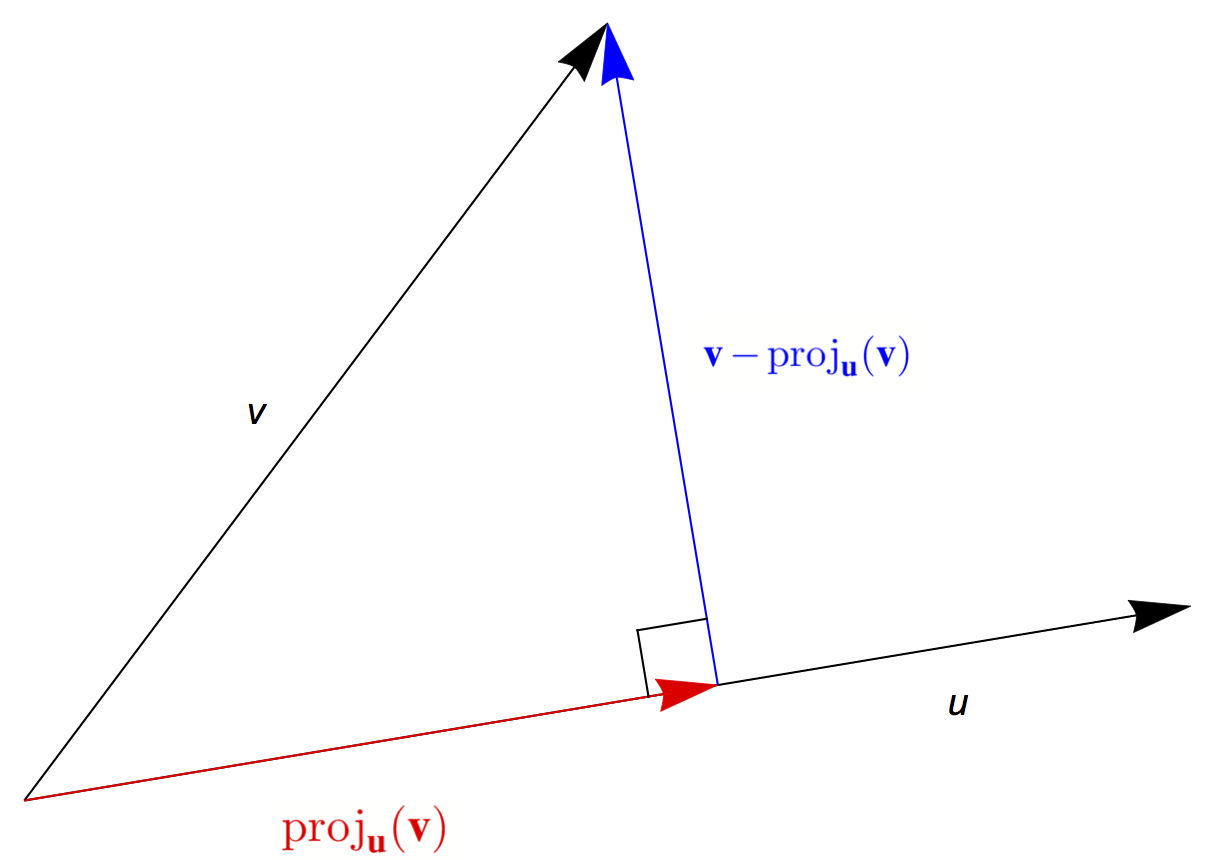
\includegraphics[width=3in]{img/decomp.jpg}
\end{center}
\caption{Orthogonal projection of $\vv$ on $\uu$.}\label{orthoprojonvector}
\end{figure}
As a result, we have \stress{decomposed} $\vv$ as a sum
$$
\vv = (\proj_{\uu}(\vv))+ (\vv-\proj_{\uu}(\vv))
$$
of something parallel to $\uu$ and something perpendicular to $\uu$,
as in our picture.

So how do we find $\proj_{\uu}(\vv)$?  It turns out to be easy.
Using either trigonometry, or just solving directly from the above
two conditions, you get:
$$
\proj_{\uu}(\vv) = \frac{\vv \cdot \uu}{\Vert \uu \Vert^2} \uu.
$$\label{projR3}
(Careful: the quotient is just a scalar.  To remember this:
if you are projecting
onto $\uu$ your answer is always a multiple of $\uu$, which is
also the term that appears in the denominator.) 

\begin{myexample}
Let $\uu = (1,0,0)$ and $\vv = (2,3,4)$.  Write $\vv$ as a sum
of two vectors, one parallel to $\uu$ and one orthogonal to $\uu$.
(Presumably you could guess the answer to this one, but let's
see what the formula does.)  We calculate:
$$
\proj_{\uu}(\vv) = \frac{\vv \cdot \uu}{\Vert \uu \Vert^2} \uu
= \frac{2+0+0}{1^2+0^2+0^2}\mat{1\\0\\0} = \mat{2\\0\\0}
$$
and $\vv - \proj_{\uu}(\vv) = (2,3,4)-(2,0,0) = (0,3,4)$, so our
decomposition is
$$
\vv = \mat{2\\3\\4} = \mat{2\\0\\0}+\mat{0\\3\\4}
$$
and it's clear that the first is parallel to $\uu$ while the 
second is orthogonal to $\uu$ --- and that this is the only
possible pair of vectors that satisfy this.
\end{myexample}

\begin{myexample}
Let $\uu = (1,1)$ and $\vv = (2,3)$.  Then
$$
\proj_{\uu}(\vv) = \frac{\vv \cdot \uu}{\Vert \uu \Vert^2} \uu
= \frac{2+3}{1^2+1^2}\mat{1\\1} = \mat{5/2\\ 5/2}
$$
is the projection of $(2,3)$ onto $(1,1)$.
\end{myexample}

Orthogonal projection is used in UMTS (Universal Mobile Telecommunications System) to correct fuzziness and errors in signals and produce more reliable
communications.

Another way of talking about orthogonal projection is to say that
we are finding the closest point to $\vv$ on the line from the origin in
direction $\uu$.  So our next goal is to talk about lines and planes.



   
\section*{Problems}
\addcontentsline{toc}{section}{Problems}

Those marked with a $\star$ have solutions at the back of the book. Try them yourself first.

\begin{prob}
\label{prob02.1}
Write down the zero vector in $\R^2$, $\R^3$ and $\R^5$.
\end{prob}

\begin{prob}
\label{prob02.2}
Prove that $\uu + (\vv + \ww) = (\uu + \vv) + \ww$ for any $\uu,\vv,\ww\in\R^3$.
\end{prob}
 

\begin{prob}
\label{prob02.3}\sov If $A=(1,\ 2,\ 3),\ B=(-5,\ -2,\ 5),\ C=(-2,\ 8,\ -10)$
and $D$ is the midpoint of $\overline{AB}$, find the coordinates of the
midpoint of $\overline{CD}$.
% $(-2,\ 4,\ -3)$

\end{prob}
\begin{prob}
\label{prob02.4} Solve the following problems using the dot product.\medskip
\begin{enumerate}[a)]



\item  Find all values of $k$ such that $(k,\ k,\ 1)$ and $(k,\ 5,\
6)$ are orthogonal.  \medskip
% -3 and -2
\item\sov Find the angle between the vectors $ (0,\ 3,\ -3)$
and $ (-2,\ 2,\ -1)$.  \medskip
%  $\pi/4$ 
\item If $A=(2,\ 4,\ 1),\ B=(3,\ 0,\ 9)$ and $C=(1,\ 4,\
0)$, find the angle $ \angle BAC$.  \medskip
% $3\pi/4$




\end{enumerate}




\end{prob}
\begin{prob}
\label{prob02.5}\sov  Solve the following problems. \medskip
\begin{enumerate}[a)]

\item If $\uu=(2,\ 1,\ 3)$ and $\vv=(3,\ 3,\ 3)$ find
 $\proj_{\vv}{\uu}$.  \medskip
%${{2}\over{3}}(3,\ 3,\ 3)$
\item   If $\uu=(3,\ 3,\ 6)$ and $\vv=(2,\ -1,\ 1)$ find
$\|\proj_{\vv}{\uu}\|$. \medskip
%$(3\sqrt6)/2$
\end{enumerate}

\end{prob}



 

 
 
\chapter{Lines and Planes}
\label{Chapter:03linesplanes}

In the last chapter we discussed the algebra and geometry of vectors in
$\R^2$ and $\R^3$, and extended all the notions of vector addition,
scalar multiplication, the dot product, angles and orthogonality
to $\R^n$.  

Now, let's consider lines and planes in $\R^2$ and $\R^3$.  
We'll see that while some ideas generalize easily
to $\R^n$, others take more work; in fact, working out what, exactly,
a reasonable analogue of a line or a plane in $\R^n$    
is one of our goals in this course.


\section{Describing Lines}

A line in $\R^2$ or $\R^3$ 
is completely determined by specifying its direction and
a point on the line.  Since we prefer working with vectors, replace
the point by its position vector.

\begin{figure}
\begin{center}
\vglue-.7cm

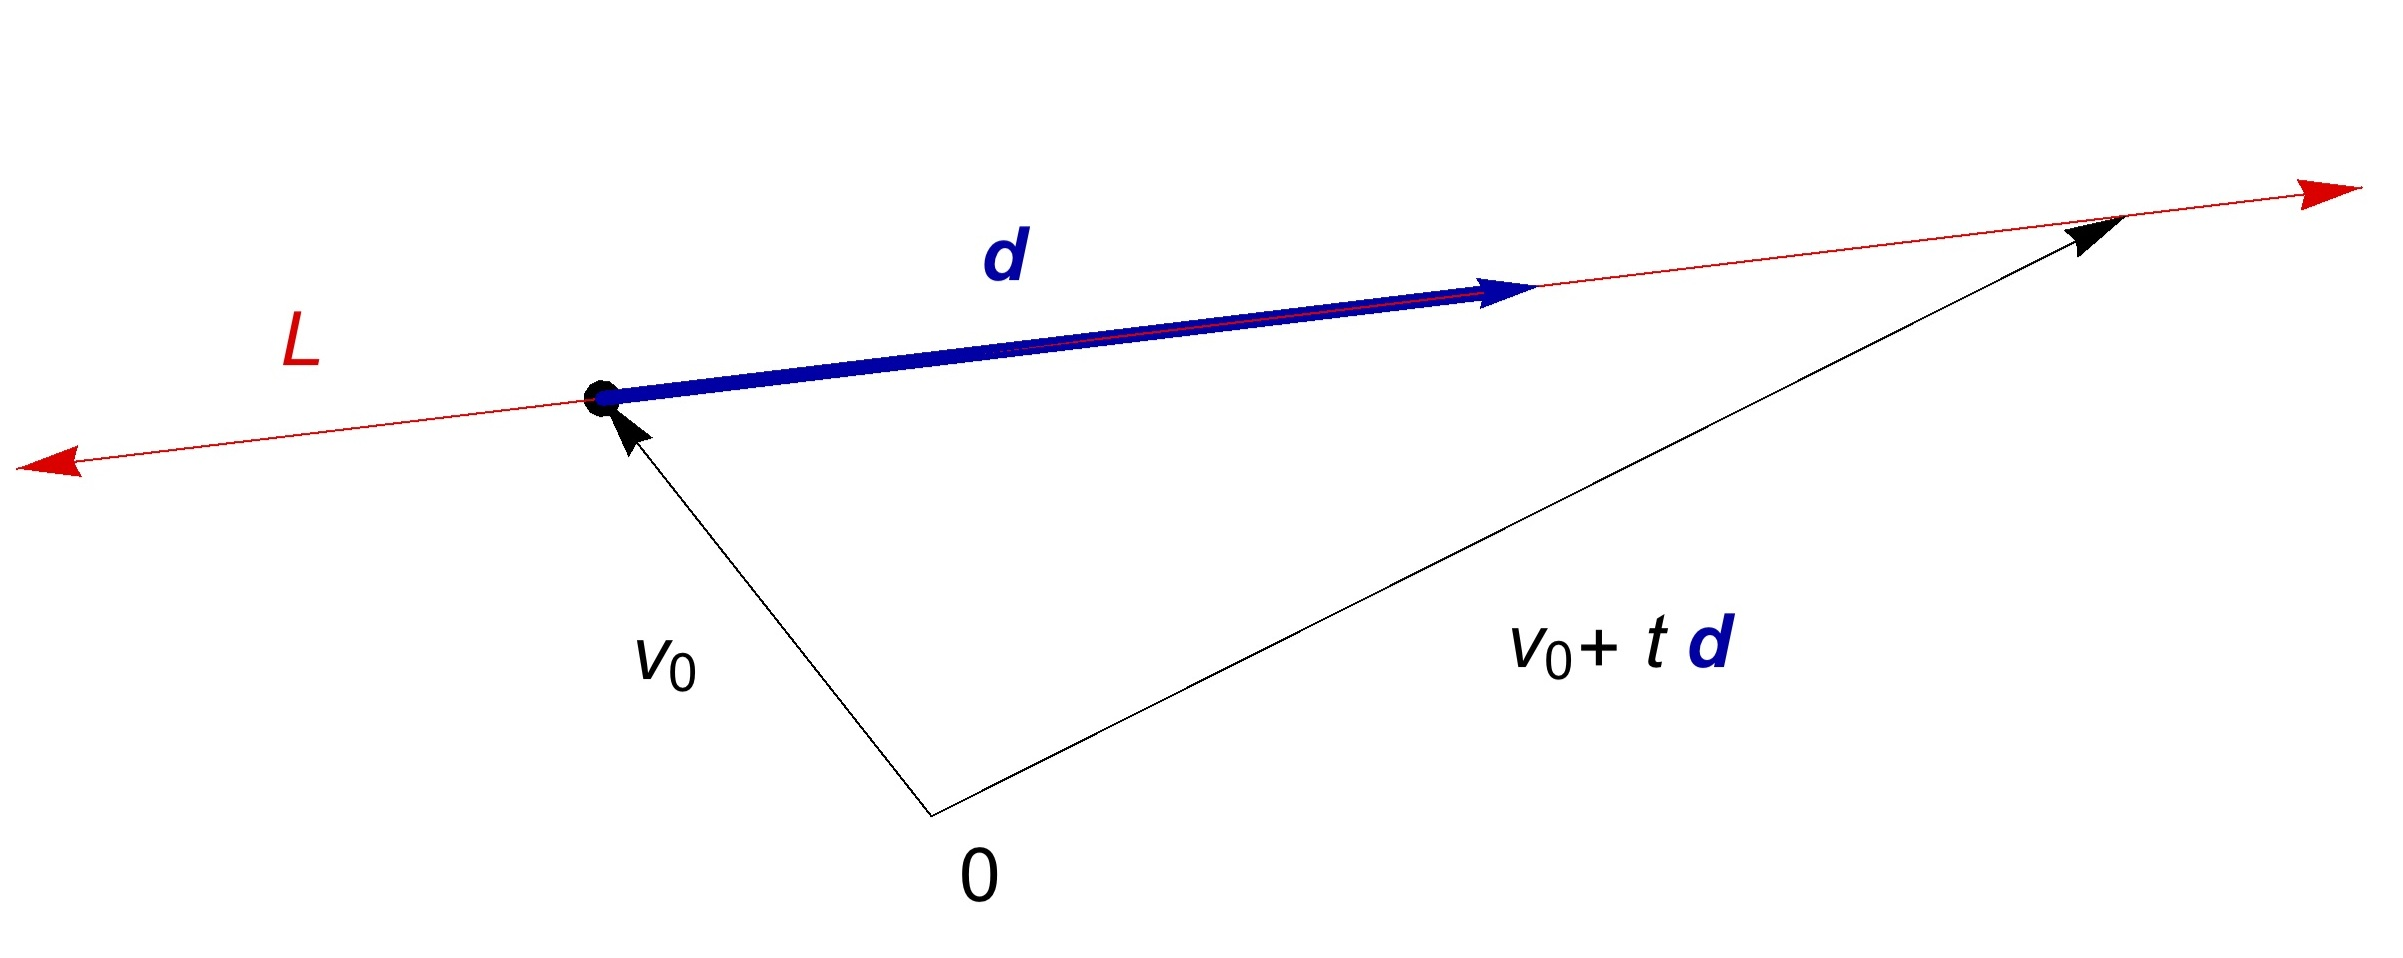
\includegraphics[scale=.1]{img/linepoint-directionvector.jpg}
\end{center}

\caption{Vector parametric form for $L$}\label{vectorparametricformplane}
\end{figure}


So a line $L$ going through the tip of $\vv_0$ and such that $\dd$
is a vector parallel to the direction of $L$ can be described as
the set
$$
L = \{ \vv_0 + t \dd | t\in \R\}.
$$
That is, any point $\vv$ on the line $L$ can be written as $\vv = \vv_0+t\dd$ for some $t$.

\begin{myexample}
Consider the line $y=3x+2$ in $\R^2$.  We can get a parametric equation for
this line by letting $x=t$ be the parameter and solving for $y$; this gives
$x = t$ and $y=3t+2$.  In vector form, this is
$$
\mat{x\\y} = \mat{t\\3t+2} = \mat{0+1t\\2+3t} = \mat{0\\2} + t\mat{1\\3}
$$
so the line is
$$
L = \left\{ \mat{0\\2} + t\mat{1\\3} \Big| \, t \in \R\right\}.
$$


Note:  Another way to get a parametric equation for this line:  it
 goes through the points $(0,2)$ and $(-\frac{2}{3},0)$,
for example.  So a direction vector is
$$\dd = \mat{0\\2}-\mat{-2/3\\0} = \mat{2/3\\2}.$$
We can take $\vv_0 = (0,2)$.  So we get
$$
L = \left\{ \mat{0\\2} + t\mat{2/3\\2} \Big|\, t\in\R\right\}.
$$
NOTICE  that our answer is not unique!  It depends on our choices.
BOTH of our answers are completely correct (check with a sketch!).
\end{myexample}

CAUTION!!  We often use the variable $t$ for the parameter.  But if
you are comparing two different lines, you must use different
letters to represent parameters on different lines!

\begin{myexample}
Find the point of intersection of $L = \{ t(1,2) | t \in \R\}$
and $L' = \{ (0,1)+t(3,0) | t \in \R\}$.

WRONG METHOD: Set $t(1,2)=(0,1)+t(3,0)$ and solve for $t$.

This doesn't give an answer for $t$; but that's only because
the two lines don't arrive at the point of intersection at
the same time $t$.  The lines still intersect!

CORRECT METHOD:  Find parameters $s$ and $t$ such that
 $t(1,2) = (0,1)+s(3,0)$.  This gives $t=\frac12$ and $s=\frac16$,
and the point of intersection is thus $(\frac12,1)$.
\end{myexample}

The form
$$
L = \{ \vv_0 + t \dd | t\in \R\}
$$
for a line in $\R^n$ is called the \defn{vector form} or \defn{parametric 
form}.  In $\R^2$ (but NOT $\R^3$), you can describe a line by an equation like
$ax+by=c$; this is called the \defn{point-normal} or \defn{Cartesian form}.

You can also expand the parametric form in coordinates:  if $\vv_0 = (a,b,c)$ and $\dd = (d_1,d_2,d_3)$ then our line
is the set of all $\vv=(x_1,x_2,x_3)$ such that 
\begin{align*}
x_1 &= a+ td_1\\
x_2 &= b+td_2\\
x_3 &= c+td_3
\end{align*}
for some $t\in \R$.

\section{About the Geometry of Lines}

There is only one line in $\R$:  all of $\R$.

Given two distinct lines in $\R^2$, they are either parallel or they intersect.

Given two distinct 
lines in $\R^3$, they could be parallel, or they could intersect,
or they could be skew.  In the first two cases, they are contained
in a unique plane; in the third case there is no plane containing
both of them (but you can find two parallel planes such that each
contains one of the lines).

\section{Describing Planes in \texorpdfstring{$\R^3$}{R3}}
Recall that planes in $\R^3$ are described by an equation in point-normal
 or  Cartesian form.  That is, a plane is described as 
the set of all points $(x,y,z)$ such that
$$
ax+by+cz = d
$$
where $\nn = (a,b,c)$ is a \emph{normal vector} to the plane
and $d\in \R$.

How did we get this equation? Look below. If $\vv_0$ is some point on the plane, then $\vv$ is on the plane iff $(\vv - \vv_0) \cdot \nn = 0$:  \begin{figure}
\begin{center}
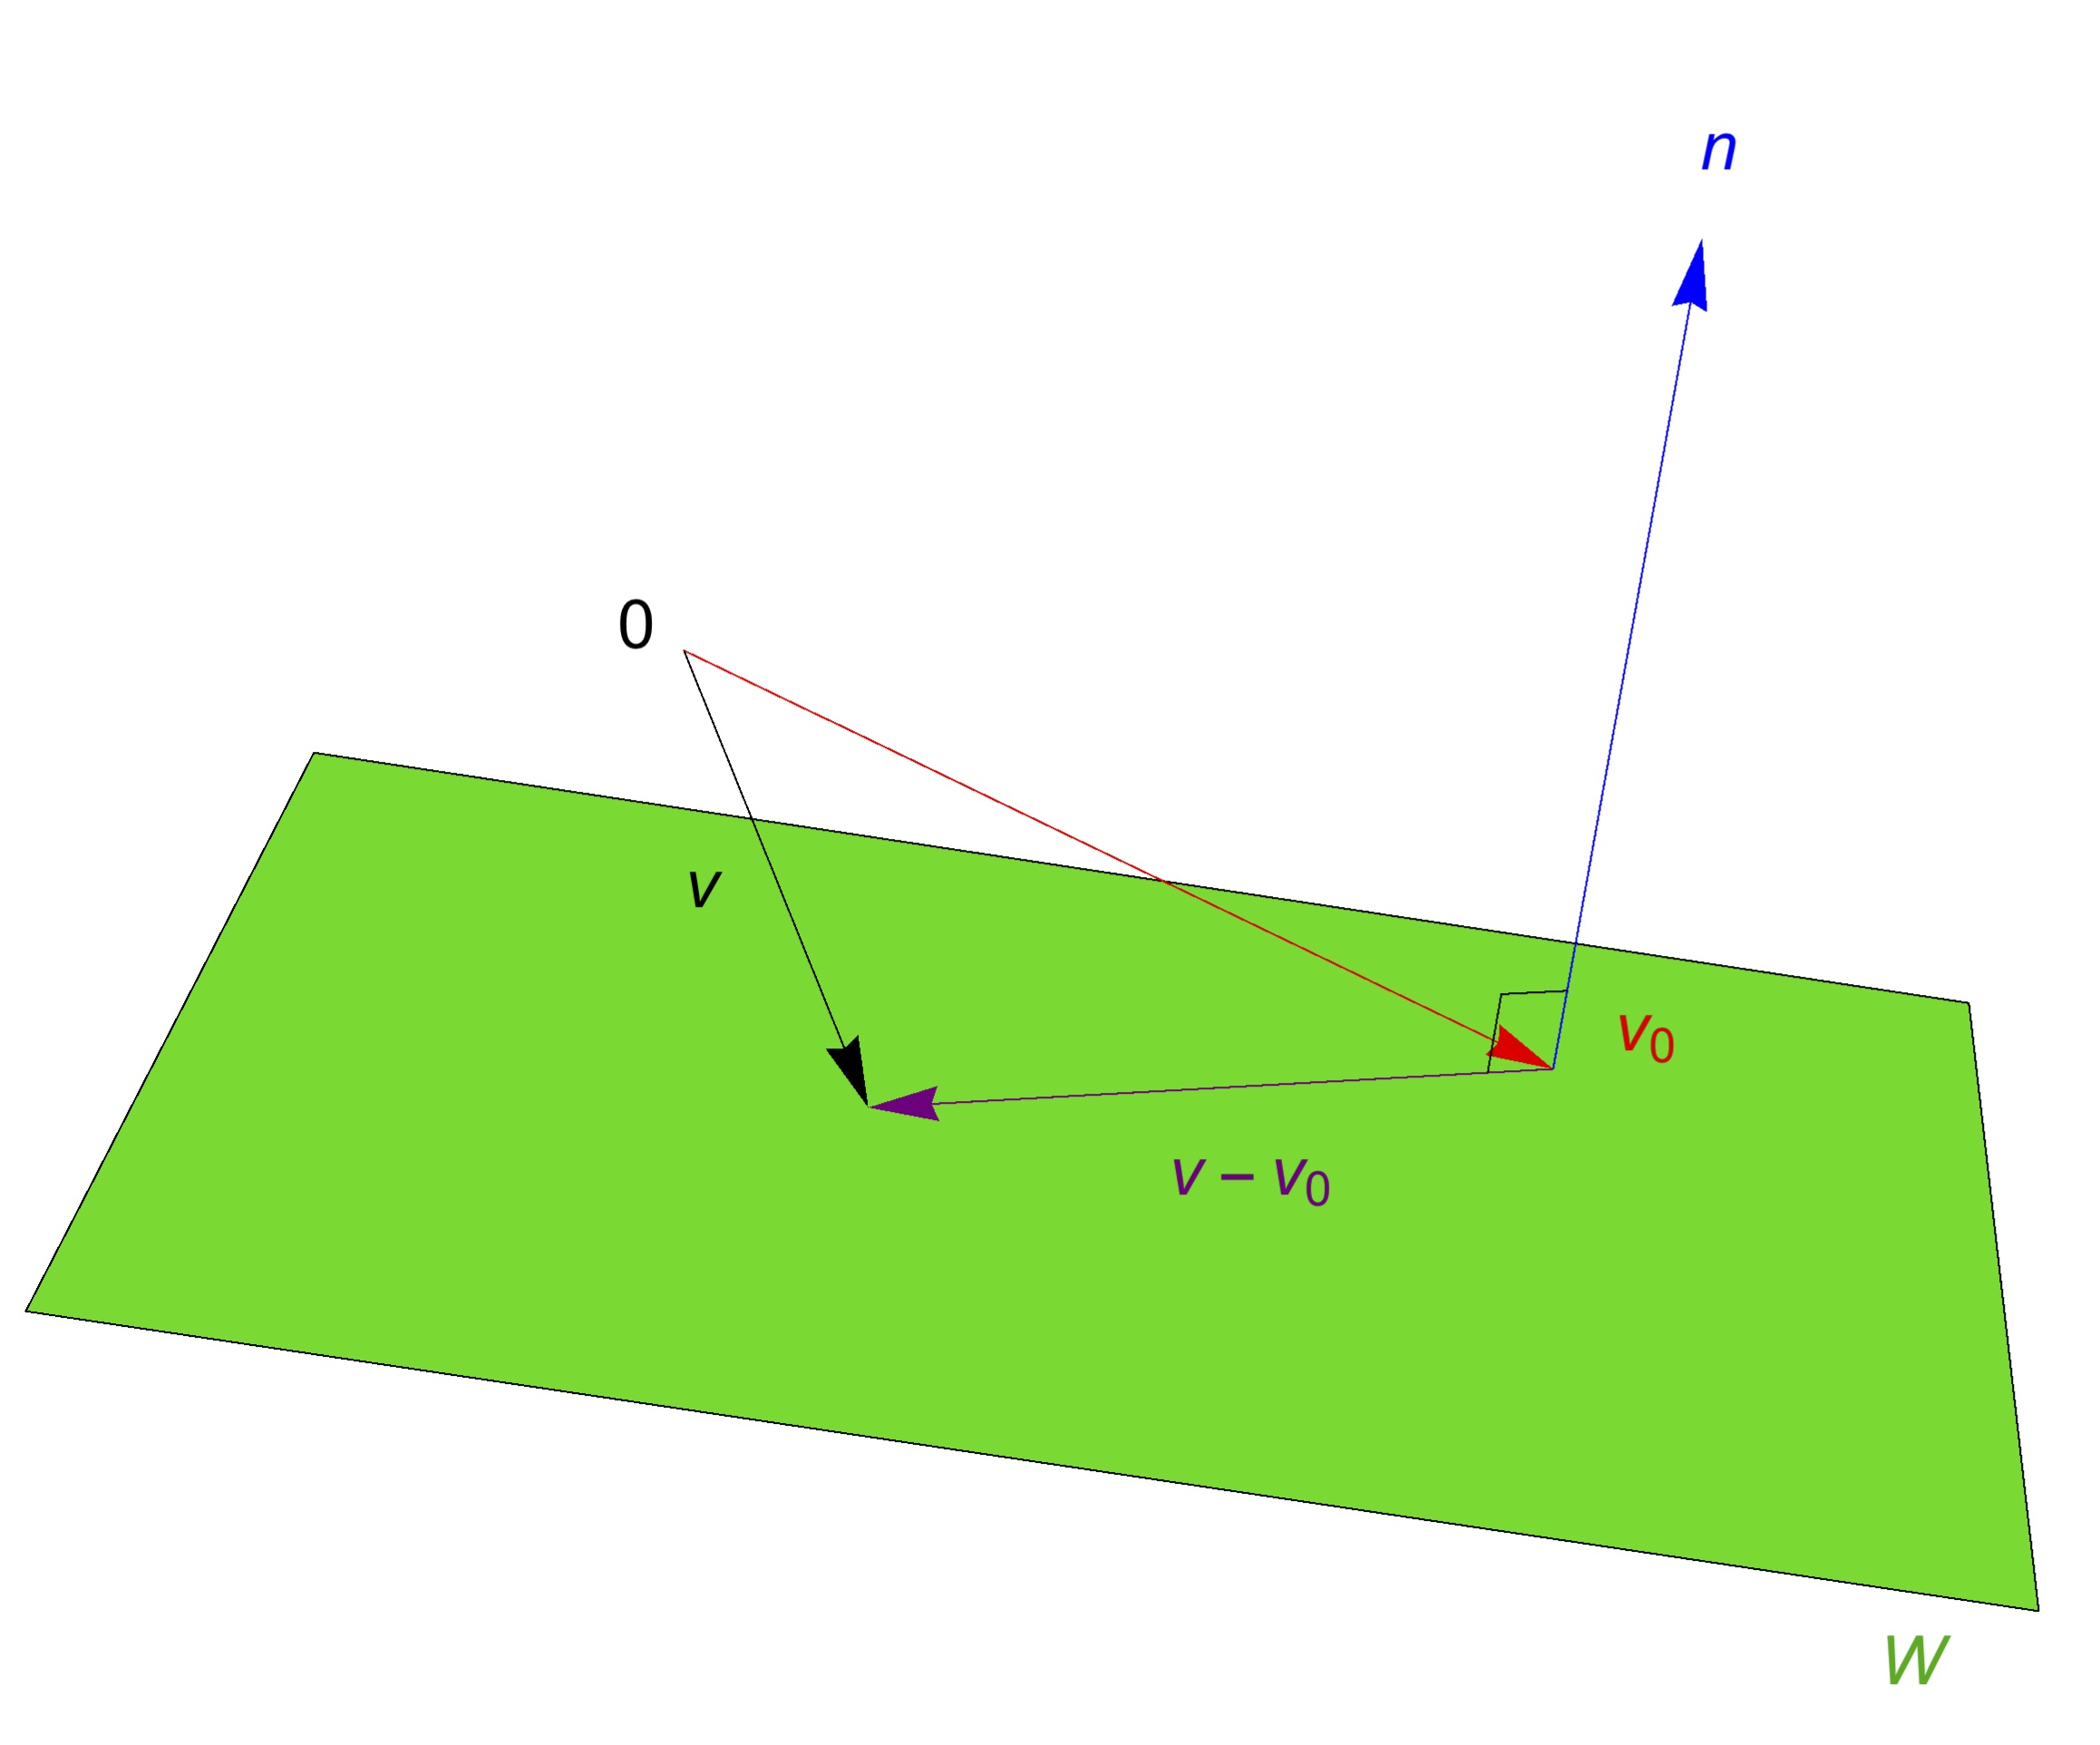
\includegraphics[width=4in]{img/cartesianequationplane.jpg}
\end{center}

\caption{The cartesian equation of a plane: point-normal form}\label{cartesiannormalformplane}
\end{figure}

So the plane through $\vv_0$ with normal vector $\nn$ is
$$
W = \{ \vv \in \R^3 | (\vv - \vv_0) \cdot \nn = 0 \}.
$$

\begin{myexample}
The plane through $\vv_0 = (1,0,3)$ with normal vector $\nn = (-1,1,2)$
is
\begin{align*}
W &= \{ \vv \in \R^3 | (\vv-\vv_0)\cdot \nn=0\}\\
&= \{ (x,y,z) | ((x,y,z)-(1,0,3))\cdot (-1,1,2)=0\}\\
&= \{ (x,y,z) | -(x-1)+(y-0) + 2(z-3) = 0\}\\
&= \{ (x,y,z) | -x+y+2z = 5\}
\end{align*}
(Note that the coefficients in the Cartesian equation give you a normal vector.)
\end{myexample}

The normal vector is handy for many things.

\begin{myprob} 
Find the distance from the point $P = (1,2,3)$
to the plane $W$ with Cartesian equation $3x-4z=-1$.

\begin{mysol} 
%\begin{figure}



%\end{figure}
Let $A$ be any point on the plane, say $A=(1,0,1)$, and $Q$ be the (unknown) closest point on the plane to $P$.
As the diagram suggests\footnote{And here's a proof, for the properly skeptical reader: if $Q'$ is any other point on $W$, $\|P-Q'\|^2=\|P-Q+ Q-Q'\|^2= \|P-Q\|^2+ \|Q-Q'\|^2$ (because $P-Q$ and $Q-Q'$ are perpendicular, so the Pythagorean theorem applies). Hence $\|P-Q'\|^2\ge  \|P-Q\|^2$. }, we want the length of the projection of $A-P$ onto the normal vector.

\begin{center}


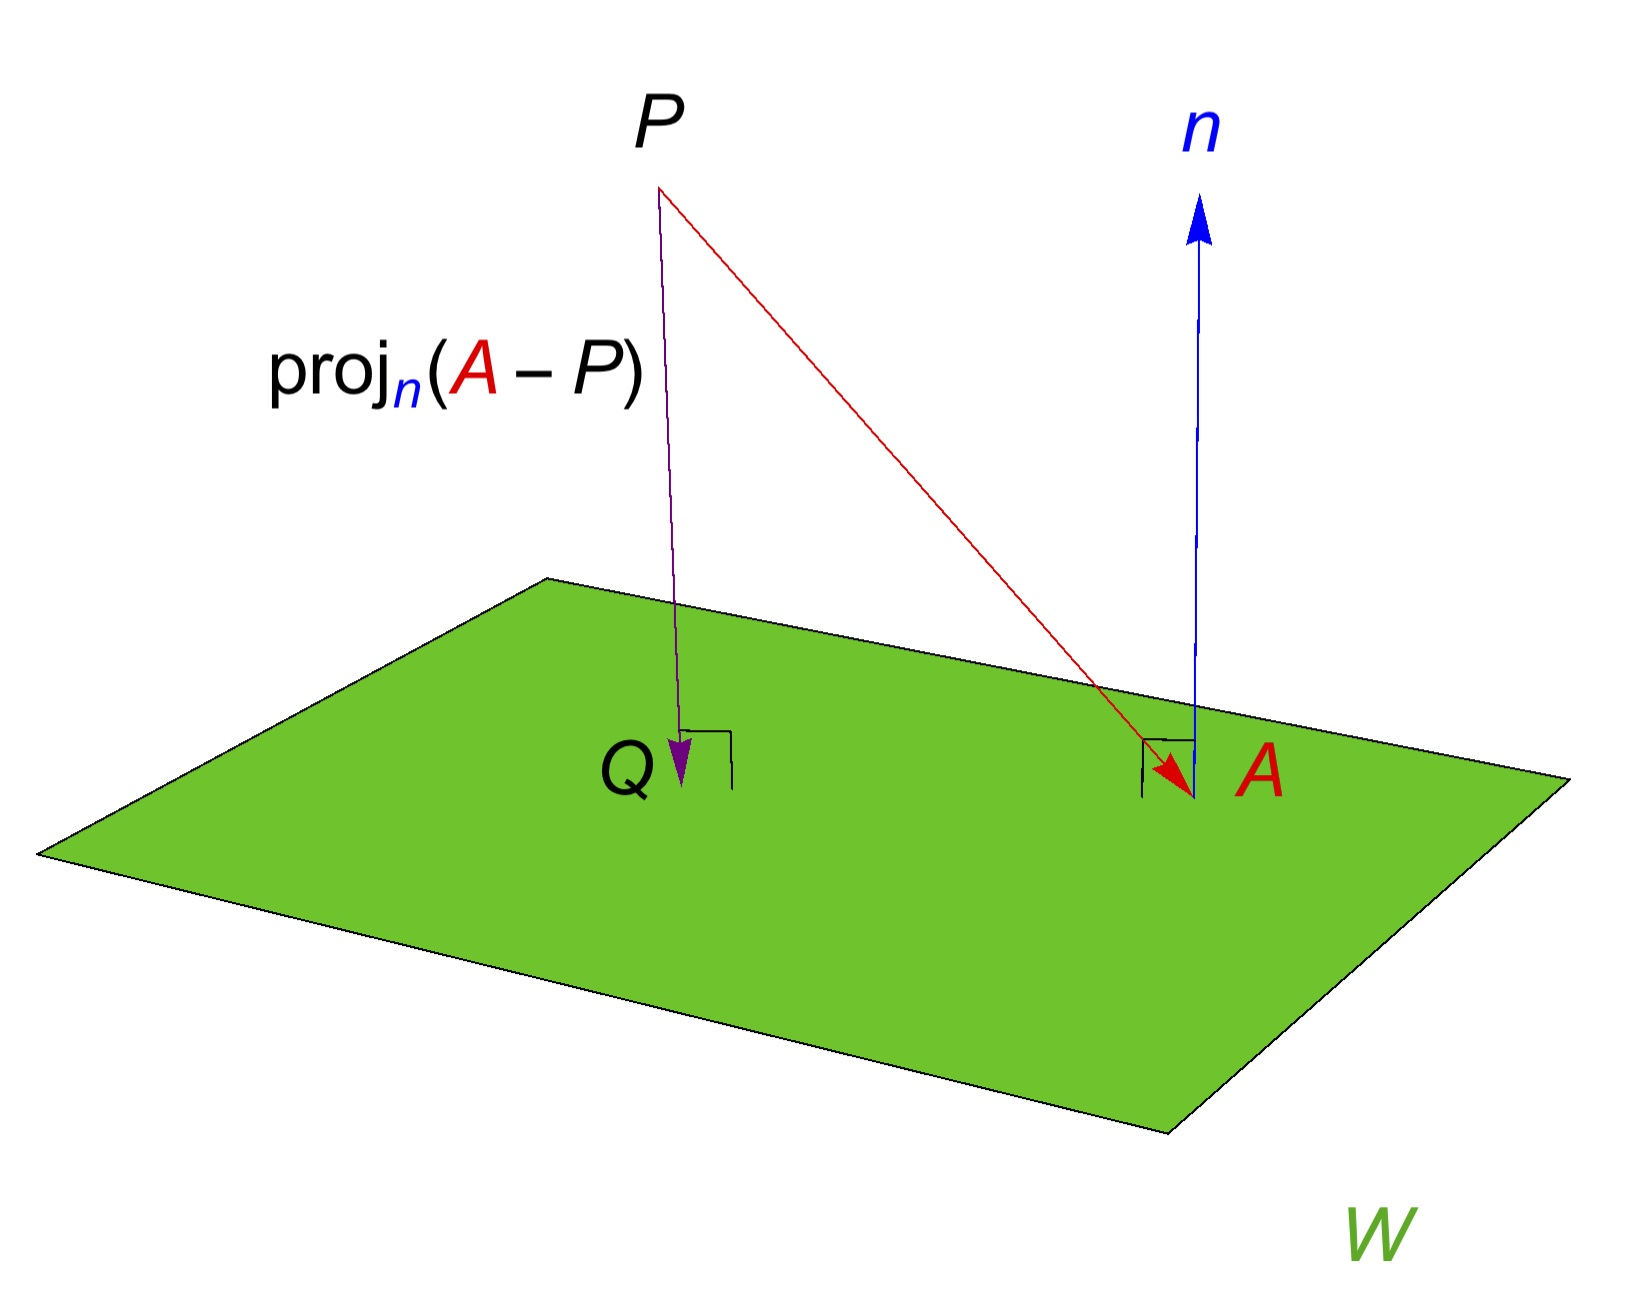
\includegraphics[scale=.5] {img/projP_on_W.jpg}

{Finding the distance of P to the plane $W$.} 
\end{center}


So
\begin{align*}
\Vert P-Q \Vert &= \Vert {\proj}_{\nn}(P-A) \Vert\\
&= \Vert {\proj}_{(3,0,-4)}(0,2,2) \Vert\\
&= \Vert \frac{0+0-8}{3^2+(-4)^2}(3,0,-4) \Vert\\
&= \frac{8}{25} \Vert (3,0,-4) \Vert\\
&= \frac{8}{25} \sqrt{25} = \frac{8}{5}.
\end{align*}
\end{mysol}
\end{myprob}

Let's tackle a more straightforward problem: the intersection of
two planes.

\begin{myprob} Find the intersection of the planes $x+y+z = 3$ and $x-y-z=2$.

\begin{mysol} We need to find all $(x,y,z)$ which satisfy both equations.
Subtracting the second equation from the first yields $2y+2z = 1$
or $y = \frac12-z$; then from the first we have $x = 3-(\frac12-z)-z
= \frac52$.  But $z$ can be anything; in fact we can take
$z$ to our parameter (and so now call it $t$):
$$
x = \frac52, \quad y=\frac12-t, \quad z=t
$$
which in vector form is the line
$$
L= \left\{ \mat{5/2\\1/2\\0} + t \mat{0\\-1\\1} | t\in \R\right\}.
$$
\end{mysol}\end{myprob}

\section{Geometry of Planes in \texorpdfstring{$\R^3$}{R3}}

We define the ``angle'' between two planes to
be the angle between their normal vectors.  It equals
the angle of the ``wedge'' that they make (although
proving that takes some thought).

Now, to compare with the case of lines:
 
The only plane in $\R^2$ is all of $\R^2$.

Given two distinct planes in $\R^3$, they are either parallel
or they intersect.

Makes you wonder about $\R^4$, doesn't it?

That said, we don't have a good way to describe a plane in $\R^4$
(yet).  
A parametric equation in one variable gives a line, in any
$\R^n$.  But something fishy is happening with the normal
forms:

\begin{center}
\begin{tabular}{cccc}
$n$ & & Equation in $\R^n$& Resulting Geometric Object \\
\hline
1 &\hphantom{XX} & $ax=b$ & point \\
2 & & $ax+by=c$ & line \\
3 & & $ax+by+cz =d$ & plane\\
4 & & $ax_1+bx_2+cx_3+dx_4=e$ & ??
\end{tabular}
\end{center}

Idea:  one equation is cutting down one \stress{degree of freedom}
(later: \defn{dimension}), so the result is always an object
of \stress{dimension $n-1$} (which is called a \defn{hyperplane} in dimensions bigger than 3).

Our answer will eventually be:  Since intersecting two planes in $\R^3$
(usually) gives you a line, intersecting two hyperplanes in $\R^4$ should
give you a plane.


This is something we'll be coming back to over the next
few weeks.


But for now: let's get back to solid ground (or rather, $\R^3$) and
discuss how to produce normal vectors to planes fairly easily.

\section{Cross products in \texorpdfstring{$\R^3$}{R3}}


Let's use the notation:
$$
\hat{i} = \mat{1\\0\\0}, \quad \hat{j} = \mat{0\\1\\0}, \quad \hat{k} = \mat{0\\0\\1}.
$$
Then $(x,y,z) = x\hat{i} + y\hat{j} + z\hat{k}$.

In the following, we also use notation from the \emph{determinant}
which for now is just very convenient.

The \defn{cross product} of $\uu = (x,y,z)$ and $\vv=(x', y', z')$
is a new vector, denoted $\uu \times \vv$, which is calculated 
as follows:
\begin{align*}
\uu \times \vv &= \left| \begin{matrix}
\hat{i} & \hat{j} & \hat{k} \\
x & y & z\\
x' & y' & z' \end{matrix} \right|\\
&= \left( yz' - y'z, -(xz' - x'z), xy' - x'y \right) \\
&= \left( \left| \begin{matrix} y & z\\ y' & z' \end{matrix} \right|,
- \left| \begin{matrix} x & z\\ x' & z' \end{matrix} \right|,
\left| \begin{matrix} x & y\\ x' & y' \end{matrix} \right| \right)
\end{align*}

\begin{myprob}
Find $(1,2,3)\times(4,5,6)$.

\begin{mysol}  Write this as a determinant (or at least on top of each other)
and then solve:
$$
\left| \begin{matrix}
\hat{i} & \hat{j} & \hat{k} \\
1 & 2 & 3\\
4 & 5 & 6 \end{matrix} \right|
= (12-15, -(6-12), 5-8) = (-3,6,-3). 
$$
\end{mysol}\end{myprob}

\begin{myprob} Find $(4,5,6)\times(1,2,3)$.

\begin{mysol} Same process:
$$
\left| \begin{matrix}
\hat{i} & \hat{j} & \hat{k} \\
4 & 5 & 6\\
1 & 2 & 3 \end{matrix} \right|
= (15-12, -(12-6), 8-5) = (3,-6,3)
$$
HA!  We got the NEGATIVE. 
\end{mysol}\end{myprob}

Notice, though, that
$$
(1,2,3)\cdot (3,-6,3) = 3-12+9 = 0, \quad (4,5,6)\cdot (3,-6,3) = 12-30+18=0.
$$
None of this was just luck.

\begin{theorem}[Properties of the Cross Product]
Let $\uu,\vv,\ww\in \R^3$.  Then
\begin{itemize}
\item $\uu \times \vv = -\vv \times \uu$
\item $(\uu \times \vv)\cdot \uu = 0$
\item $(\uu \times \vv)\cdot \vv = 0$
\item $(\uu + \vv)\times \ww = \uu \times \ww + \vv \times \ww$
\item $\Vert \uu \times \vv \Vert = \Vert \uu \Vert \; \Vert \vv \Vert \sin(\theta)$ where $0 \leq \theta \leq \pi$ is the angle between $\uu$ and $\vv$.
This is in fact the area of the parallelogram with sides $\uu$ and $\vv$.
\end{itemize}
BUT, usually:  $\uu \times (\vv \times \ww) \neq (\uu \times \vv) \times \ww$;
the cross product is neither commutative nor associative.  (Eg:  $\hat{i} \times (\hat{k} \times \hat{k}) = \zero$ but $(\hat{i} \times \hat{k})\times \hat{k} = -\hat{i}$.)
\end{theorem}


Consequently:
if two vectors are parallel, then their cross product
is zero.  Otherwise, their cross product is one of the two vectors orthogonal to both 
$\uu$ and $\vv$ and of length $\Vert \uu \Vert \; \Vert \vv \Vert \sin\theta$, where $\theta$ is the angle between $\uu$ and $\vv$.
The cross product is used in Physics for measuring torque, for example,
and figuring out the direction of the answer uses the
right-hand rule.  We also often memorize $\hat{i} \times \hat{j} = \hat{k}$ and its cyclic permutations.

\section{First application of cross product: finding normal vectors}

The cross product gives a normal vector to the plane parallel to two vectors $\uu$ and $\vv$.

\begin{myprob}
Find an equation of the plane containing the three points $A = (1,2,3)$,
$B = (1,0,0)$ and $C = (0,1,1)$.

\begin{mysol}
The vectors $\vec{BA} = (0,2,3)$ and $\vec{BC} = (-1,1,1)$ are both
parallel to the plane, so a normal vector to the plane must be
orthogonal to each of these.  So take their cross product:
$$
 \left| \begin{matrix}
\hat{i} & \hat{j} & \hat{k} \\
0 & 2 & 3\\
-1 & 1 & 1 \end{matrix} \right| = (-1, -3, 2)
$$
(Check your answer!  This should be orthogonal to $\vec{BA}$
and $\vec{BC}$.)

So an equation for the plane has the form
$$
-x -3y + 2z = d
$$
and plugging in the point $B$, for example, yields $d=-1$.
\end{mysol}\end{myprob}

\section{Second Application:  volumes of parallelepipeds (Scalar Triple Product)}

\begin{theorem}[Volume of a parallelepiped]
The volume of the parallelepiped with sides $\uu$, $\vv$ and $\ww$
in $\R^3$ is
$$
\vert (\uu \times \vv) \cdot \ww \vert. 
$$
In particular, the order of the vectors doesn't matter.
\end{theorem}

We can prove this using more trigonometry:  the volume of
the parallelepiped is the area of the base (a parallelogram)
times the height; the area of the base is the norm of the cross product
of two of the vectors ($\Vert \uu \times \vv \Vert$), and the height is going to be 
$\Vert \ww \Vert \cos(\theta)$ where $\theta$ is the angle between
$\ww$ and a normal vector to the base.

\begin{myprob}
Find the volume of the parallelepiped with sides $\uu = (1,0,1)$,
$\vv = (1,2,2)$ and $\ww = (10,0,0)$.

\begin{mysol}
We calculate:
$$
\uu \times \vv =  \left| \begin{matrix}
\hat{i} & \hat{j} & \hat{k} \\
1 & 0 & 1\\
1 & 2 & 2 \end{matrix} \right| 
= (-2,-1,2)
$$
so
$$
(\uu \times \vv)\cdot \ww = (-2,-1,2)\cdot (10,0,0) = -20
$$
so the volume is $20$.
\end{mysol}\end{myprob}

So what does it mean if $(\uu \times \vv)\cdot \ww = 0$?  Zero
volume of a parallelepiped means it wasn't really a parallelepiped
at all --- the three vectors must all lie in a plane.  We
say such vectors are \defn{coplanar} or \defn{linearly dependent}
(key phrase for later).





\section{Final remarks about lines, planes, and higher-dimensional
objects in \texorpdfstring{$\R^n$}{Rn}}  

These are just some thoughts to preview some of the ideas
we want to explore over the next several weeks.  We have
great ways to describe lines and planes in $\R^2$ and $\R^3$,
but we have an inkling that there must be ``2-dimensional'' objects
in $\R^4$ which we can't describe by either of the two
methods described so far (parametric equations or normal equations).

Or can we?  

To get a line,
we gave ourselves one parameter (one degree of freedom).  If
we give ourselves two parameters, for two different direction
vectors, this describes a plane.  That is
$$
W = \{ \vv_0 + s\dd_1 + t\dd_2 | s,t\in\R\}
$$
describes the plane with normal vector $\dd_1 \times \dd_2$
and going through the point $\vv_0$.

We will explore statements like this in the course of understanding
subspaces of general vector spaces.





\section*{Problems}
\addcontentsline{toc}{section}{Problems}


    
 
\begin{prob}\label{prob03.1}  Solve the following problems using the cross and/or dot products.\medskip
\begin{enumerate}[a)]
\item If $\uu=(3,\ -1,\ 4)$ and $\uu=(-1,\ 6,\ -5)$, find
$\uu\times \vv$. \medskip
% $(-19,\ 11,\ 17)$
\item\sov Find all vectors in $\R^3$ which are orthogonal to both  $(-1, 1, 5)$ and $(2, 1, 2)$.  \medskip
% $\{(t,\ -4t,\ t)|\ t\in \R\}$
\item  If $\uu=(4,\ -1,\ 7),\ \vv=(2,\ 1,\ 2)$ and 
$\ww=(-1,\ -2,\ 3)$, find $(\uu\times \vv)\times \ww$. \medskip
% $(30,\ 21,\ 24)$
\item\sov If $\uu=(-4,\ 2,\ 7),\ \vv=(2,\ 1,\ 2)$ and 
$\ww=(1,\ 2,\ 3)$, find $\uu\cdot (\vv\times \ww)$. \medskip
% 17
\end{enumerate}

\end{prob}
\begin{prob}
\label{prob03.2}  Solve the following problems using the appropriate products.\medskip
\begin{enumerate}[a)]

\item Find the area of the parallelogram determined by the vectors
$\uu=(1,\ -1,\ 0)$ and $\vv=(2,\ -3,\ 1)$.    \medskip
%
\item\sov Find the area of the triangle with vertices $A=(-1,\ 5,\
0)$, $B=(1,\ 0,\ 4)$ and $C=(1,\ 4,\ 0)$.  \medskip
%6
\item Find the area of the triangle whose vertices are $P=(1,\
1,\ -1),\ Q=(2,\ 0,\ 1)$ and $R=(1,\ -1,\ 3)$.  \medskip
%\sqrt{5}


\item\sov Find the volume of the parallelepiped  determined by $\uu=(1,\ 1,\ 0),\ \vv=(1,\ 0,\ -1)$ and $\ww=(1,\ 1,\ 1)$.\medskip
% 1

\item Find the volume of the parallelepiped  determined by $\uu=(1, -2, 3),\ \vv=(1,3,1)$ and $\ww=(2,1,2)$.\medskip
% 10

\end{enumerate}



\end{prob} \begin{prob} \label{prob03.3}  Solve the following problems. \medskip
\begin{enumerate}[a)]
\item\sov Find the point of intersection of the plane with Cartesian equation $2x+2y-z=5$,
and the line with parametric equations $x=4-t,\ y=13-6t,\ z=-7+4t$.  \medskip
%$(2,\ 1,\ 1)$
\item\sov If $L$ is the line passing through $(1,\ 1,\ 0)$ and $(2,\
3,\ 1)$, find  the point of intersection of $L$ with the plane with Cartesian equation $x+y-z=1$. \medskip
% $(0,\ 1/2,\ -1/2)$
\item  Find the point where the lines with parametric equations $x=t-1$,   $y=6-t,\ z=-4+3t$ and $x=-3- 4t,\ y=6-2t,\ z=-5+3t$ intersect. \medskip
%(1,\ 4,\ 2)
\item\sov  Do the planes with Cartesian equations $2x-3y+4z=6$ and $4x-
6y+8z=11$ intersect? \medskip
% No
\item Find the line of intersection of the planes with Cartesian equations $5x+7y-4z=8$ and $x-y=-8$. \medskip
%$(-4,\ 4,\ 0)+ t (1,\ 1,\ 3),\, t\in \R$

\item\sov Find the line of intersection of the planes with Cartesian equations $x+11y-4z=40$ and $x -y=-8$. \medskip
%$(-4,\ 4,\ 0)+ t (1,\ 1,\ 3),\, t\in \R$

\end{enumerate}



\end{prob} \begin{prob} \label{prob03.4}  Solve the following problems. \medskip
\begin{enumerate}[a)]

\item  Find the distance from the point $(0,\ -5,\ 2)$ to the plane with Cartesian equation
$2x+3y+5z=2$. \medskip
%$7/\sqrt{38}$

\item\sov  Find the distance from the point $(-2,\ 5,\ 9)$ to the plane with Cartesian equation
$6x+2y-3z=-8$  \medskip
%3
\item Find the distance from the point $(5,\ 4,\ 7)$ to the
line containing the points $(3,\ -1,\ 2)$ and $(3,\ 1,\ 1)$.
\medskip
%



\item\sov  Find the distance from the point $(8,\ 6,\ 11)$ to the
line containing the points $(0,\ 1,\ 3)$ and $(3,\ 5,\ 4)$.  \medskip
% 7
 
\item Find angle between the planes with Cartesian equations $x-z=7$ and $y-z=234$
\medskip
%$\pi/3$




\end{enumerate}



\end{prob} \begin{prob} \label{prob03.5}  Find the scalar {\it and} vector parametric forms for  the following lines:
\medskip
\begin{enumerate}[a)]

\item The line containing $(3,\ -1,\ 4)$  and $(-1,\ 5,\ 1)$. \medskip
% 
\item\sov The line containing $(-5,\ 0,\ 1)$ and which is parallel to the two planes with Cartesian equations $2x-4y+z=0$ and  $x-3y-2z=1$ 
\medskip
%$x=-5+11t,\, y=5t,\, z=1-2t,\, t\in \R$
\item The line passing through  $(1,\ 1,\ -1)$ and which is perpendicular to the plane with Cartesian equation $2x-y+3z=4$ \medskip
%$x=1+2t,\, y=1-t,\, z=-1+3t,\, t\in \R$
\end{enumerate}

\end{prob} \begin{prob} \label{prob03.6}  Find a Cartesian equation for each of the following planes:

\medskip
\begin{enumerate}[a)]
\item The plane containing $(3, -1, 4)$, $(-1, 5, 1)$ and $(0, 2, -2)$.\medskip
% $2y - z = 3$

\item\sov  The plane parallel to the vector $(1, 1, -2)$  and containing  the points $(1, 5, 18)$ and $(4, 2, -6)$ \medskip 
%$5x - 3y + z = 8$

\item  The plane passing through the points  $(2, 1, -1)$ and $(3, 2, 1)$, and parallel to the $x$--axis. \medskip 
%
\item\sov  The plane containing the   two lines 
$ \set{(t-1,6-t,-4+3t)\st t \in \R}$ and 
 $ \set{(-3 -4t, 6+ 2t,  7+5t)\st \in \R} $    \medskip  
%$11x + 17y + 2z = 83$
\item The plane which contains the point (-1, 0, 2) and the line of intersection of the two planes $3x + 2y - z = 5$ and $2x + y + 2z = 1$.  \medskip  
%$23x + 12y + 19z = 15$
\item\sov The plane containing the point $(1, -1, 2)$  and the line \hfill \\$\set{(4, -1 + 2t,2 + t)\st t \in \R}$. \medskip
% $y - 2z + 5 = 0$
\item The plane through the origin parallel to the two vectors  $(1, 1, -1)$ and $(2, 3, 5)$.\medskip
%$8x - 7y + z = 0$
\item\sov The plane containing the point $(1,\ -7,\ 8)$ which is perpendicular to the line $\set{(2+2t,7-4t,-3+t\st  t\in \R}.$ \smallskip  
%$2x-4y+z=38$
\item The plane containing the point  $(2,\ 4,\ 3)$ and which is perpendicular to the planes with Cartesian equations $x+2y-z=1$  and $3x-4y=2$.  
% $4x+3y+10z=50$


\end{enumerate}
 

\end{prob} \begin{prob} \label{prob03.7}   Find a vector parametric form  for  the planes with Cartesian equations given as follows. (i.e. find some $a \in H$ and two non-zero, non-parallel vectors $\uu, \vv \in \R^3$, parallel to the plane $H$. Then  $H=\set{a+ s \uu + t \vv\st s,t \in \R}$.)\medskip
\begin{enumerate}[a)]

\item  $x - y - z = 3$\medskip 
%  
\item\sov $x - y - 2z = 4$ \medskip
% 
\item $2x - y + z = 5$ \medskip
% 
\item $y + 2x = -3$ \medskip
% 
\item $x - y + 2z = 0$ \medskip
% 
\item  $x + y + z = -1$\medskip
% 
\end{enumerate}


\end{prob} \begin{prob} \label{prob03.8}\sov  Let $\uu, \vv$ and $\ww$ be any vectors in $\R^3$.  Determine which  of the following statements could be false, and give an example to illustrate each of your answers.
 \medskip

(1)  $\uu\cdot \vv=\vv\cdot \uu$

(2)  $\uu\times\vv=\vv\times \uu$

(3)  $\uu\cdot(\vv+\ww)=\vv\cdot \uu+\ww\cdot \uu$

(4)  $(\uu+2\vv)\times \vv=\uu\times \vv$

(5)  $(\uu\times \vv)\times \ww=\uu\times(\vv\times \ww)$

% 2 \& 5

\end{prob} \begin{prob} \label{prob03.9}\sov  Let $\uu$, $\vv $ and $\ww $ be vectors in $\R^3$.  Which of the following
statements are (always) true? Explain your answers, including  giving examples to illustrate statements which could be false.
\medskip

(i)  $(\uu\times \vv)\cdot \vv=0$.
 

(ii)  $(\vv\times \uu)\cdot \vv=-1$.
 

(iii)  $(\uu\times\vv)\cdot \ww$ is the volume of the of the parallelepiped  determined by $\uu$, $\vv$ and $\ww$.
 

(iv)  $\Vert \uu\times \vv\Vert=\Vert \uu \Vert \, \Vert \vv \Vert\,\cos\theta$
where $\theta$ is the angle between $\uu$ and $\vv$.
 

(v)  $|\uu\cdot \vv|=\Vert \uu \Vert \, \Vert \vv \Vert\,\cos\theta$
where $\theta$ is the angle between $\uu$ and $\vv$.



\end{prob} \begin{prob} \label{prob03.10} Prove the identity $\uu \times (\vv\times \ww)= (\uu\cdot \ww) \vv -(\uu\cdot \vv) \ww$ for all $\uu,\vv,\ww \in \R^3$, as follows: Denote the difference between the left hand side of the identity  and the right hand side by $D(\uu,\vv,\ww)$.

First note that, by properties of the dot and cross products,  for all $k\in \R$, $\uu,\vv,\ww,\uu',\vv',\ww' \in \R^3$, it's easy to see that the following identities hold.
 
\medskip
\begin{enumerate}[(i)]
 
\item $D(k \uu +\uu', \vv,\ww) =k\, D(\uu,\vv,\ww) +D(\uu',\vv,\ww)$
\medskip
%

\item  $D(\uu , k \vv +\vv',\ww) =k\,D(\uu,\vv,\ww)  + D(\uu,\vv',\ww)$
\medskip
%
\item $D(\uu, \vv,k \ww +\ww') =k\, D(\uu , \vv,\ww)+ D(\uu, \vv,\ww')$
\medskip
%
\item Also: $D(\uu, \vv,\ww) =-D(\uu,\ww,\vv) $
\medskip
%
\end{enumerate}

(Properties (i)--(iii) are summarized by saying that ``{\it $D$ is  linear in each argument}''. More on this when we get to linear transformations.)
\medskip 

Now since every vector in $\R^3$ is a linear combination of $\hat i= (1,0,0), \hat j =(0,1,0)$ and $\hat k=(0,0,1)$, by the identities above, it suffices to check that  $D(\uu,\vv,\ww)=0$ when $\uu$ is  $\hat i, \hat j$ and $\hat k$, and $\vv$ and $\ww$ are one the 6 pairs of two distinct choices from $\set{\hat i, \hat j, \hat k}$. Restricted to these (18) choices, it's easy to see   $D(\uu,\vv,\ww)$ is zero unless $\uu$ is $\vv$ or $\ww$, so we really only need to check $D(\uu,\uu,\ww)=0$ in the 6 cases where  $\uu\in  \set{\hat i, \hat j, \hat k}$ and   $\ww \in\set {\hat i, \hat j, \hat k}\setminus\set{\uu}$.   This amounts to 6 easy computations. Having checked those, you're done!  
  
\end{prob} 



%----------------------------------------------------------------------------------------
%	PART II : Vector spaces
%----------------------------------------------------------------------------------------

\chapterimage{Montpellier1.jpg}
%MontpellierAqueduct7141.jpg


\renewcommand{\partintrotext}{Given that the algebra of $\R^2$ and $\R^3$  extended so easily to $\R^n$, we ask ourselves:  what other kinds of mathematical objects behave (algebraically speaking) just like $\R^n$?   We formulate this question precisely in the first
chapter, and proceed to uncover many very familiar examples.}

\part{Vector Spaces}

\chapter{Vector Spaces}
\label{chapter:04vectorspaces}

 

So far, we have established that it isn't too hard to generalize
our notion of \stress{vectors} to include elements of $\R^n$.  We
still call them \stress{vectors} even though we can no longer quite
imagine them as arrows in space.  

As we worked through vector geometry, we also saw
a number of problems coming up, principally among them:
 what are the higher-dimensional
analogues of lines and planes?  How can you describe them?

We will tackle this problem next, but it turns out that the
best way to do this is to step back and see just how far
we can generalize this notion of \stress{vector spaces} --- 
was $\R^n$ the only set that behaves substantially
like $\R^2$ and $\R^3$, or are there many more mathematical
objects out there that, if we look at them in the right
way, are just like vectors, too?

\section{A first example}
So far:  we agree that the elements of  $\R$, $\R^2$ and $\R^3$ are 
\defn{geometric vectors}.

We also agree that we can call elements of $\R^n$, for $n \geq 4$,
\defn{vectors}.

What we are looking for next:  non-geometric, non-$\R^n$ vectors.

\begin{myexample} {\bf Spaces of Equations}

Consider three equations, which we name $E_1$, $E_2$ and $E_3$:
\begin{align*}
E_1 &: \quad  &x-y-z &= -1 \\
E_2 &: \quad &2x-y+z &= 1\\
E_3 &: \quad &-x+2y+4z &=4
\end{align*}
We can create new equations from these ones; for example,
$$
E_4 = E_2-2E_1 \quad : \quad y+3z=3
$$
or
$$
E_1 + E_3 \quad : \quad y+3z = 3
$$
So we can even say
$$
E_2-2E_1 = E_1 + E_3
$$
and it is legitimate to rewrite this as:
$$
3E_1 -E_2 + E_3 = 0
$$
where ``0'' stands for the equation ``$0=0$''.

Well, what are we really saying here?
\begin{itemize}
\item We can {\bf add} two equations to get another equation.
\item We can {\bf multiply} an equation {\bf by a scalar} to get
another equation.
\item There's a {\bf zero equation} given by $0=0$.  Let's call it
$E_0$.
\item Equations have {\bf negatives}:
$$
-E_1 : -x+y+z=1
$$
Why is this the negative?  Because now $(E_1) + (-E_1) = E_0$.
\item The {\bf usual rules of arithmetic} hold:
\begin{itemize}
\item $E_1 + E_2 = E_2+E_1$
\item $E_1 + (E_2+E_3) = (E_1 + E_2) + E_3$
\item $k(E_1+E_2) = kE_1+kE_2$
\item $(k+l)E_1 = kE_1 + lE_1$
\item $(kl)E_1 = k(lE_1)$
\item $1 E_1 = E_1$
\end{itemize}
\end{itemize}


In other words:  these are {\bf exactly} the properties of $\R^n$
that we identified last week!  So even though we have no reasonable
way (yet) of writing ``equations'' as $n$-tuples of numbers, 
algebraically we recognize that they act just like vectors do.
\end{myexample}

 

\standout{Major idea \#1 (this chapter): there are lots of different vector spaces besides $\R^n$.}

We can specialize this a bit more (which also helps us start to
see the value in this approach):

Consider the space $\mathcal{E}$ of all equations ``obtainable from'' (also say:  \stress{generated by} or \stress{spanned by}) $E_1$, $E_2$, and $E_3$:
$$
\mathcal{E} = \{ k_1E_1 + k_2 E_2 + k_3 E_3 \;| \; k_i \in \R\}.
$$
(This is the set of \emph{all} linear combinations \index{linear combination} of those three equations!)
In fact, $\mathcal{E}$ itself acts like a space of vectors (in
the sense above, and to be made precise below).

The kinds of questions you'd want to ask:
Is there an equation of the form $y=y_0$ in $\mathcal{E}$? That is,
can we solve for $y$?\footnote{The 
connection is that: to solve for $y$, what you're honestly
doing is taking linear combinations of equations.}  (Or for $x$, for that matter.) 

\begin{myexample}
Can we find $a,b,y_0\in\R$ so that the equation $y=y_0$
equals $aE_1+bE_2$?  Answer: NO.  Why?  The coefficient
of $x$ in $aE_1+bE_2$ is $a+2b$ and the coefficient of
$z$ in $aE_1+bE_2$ is $-a+b$.  The only way these
can both be zero is if $a$ and $b$ are zero (check);
but then $aE_1+bE_2 = E_0$, the zero equation.  So 
we can't get an equation like $y=y_0$. \end{myexample}

(We of course want to answer tougher questions than that,
but our technique (Gaussian elimination, Chapter~\ref{chapter:11solvingsystems}) will
be based entirely on this idea of taking linear combinations
of equations.)

\defn{Stoichiometry} is the science of figuring out how to
produce a given chemical as a result of reactions of other,
easier to obtain, chemicals.  In stoichiometry, you let $\mathcal{E}$
be the set of all known chemical reactions and want to choose
a best (linear) combination of reactions which will result in
what you wanted.

 
\standout{Major idea \#2: (next two chapters): Subspaces and 
spanning sets.  To answer particular problems, we typically need to
understand the subspace spanned by some vectors.}

\section{So what do we really need?}
Idea:  \stress{vectors} don't have to be geometric, or even $n$-tuples.
But we want things that act like our known examples of vectors
\emph{algebraically}.  (Please note: we're going to ignore the
geometry (like the dot product) for quite a while; we're now
just focussing on the algebra.)

So we need: 
\begin{itemize}
\item $V$ : a set of ``vectors'' of some sort
\item a rule for ``adding'' two ``vectors'' (denoted with $+$)
\item a rule for ``scalar multiplication'' of a ``vector'' by an element $c\in \R$
\end{itemize}
such that all 10 of the following \defn{axioms} hold:
\begin{description}
\item[\it Closure] (These two axioms guarantee that $V$ is ``big enough'')\\
(1) The sum of two vectors should again be a vector.  (That is, if $\uu, \vv \in V$ then $\uu + \vv \in V$.)\\
(2) Any scalar multiple of a vector should again be a vector.  (That is, if $\uu \in V$ and $c\in \R$ then $c\uu \in V$.)
\item[\it Existence] (These two axioms guarantee that   $V$ has the `basics')\\
(3) There should be a zero vector $\zero$ in $V$; it must satisfy
$\zero + \uu = \uu$ for all $\uu \in V$.\\
(4) Every vector in $V$ should have a negative in $V$.  That is, given $\uu \in V$, there
should exist another vector $-\uu \in V$ such that $\uu + (-\uu) = \zero$.
\item[\it Arithmetic properties] (These axioms guarantee that operations behave the way they did in $\R^n$)\\
For any $\uu, \vv, \ww \in V$ and any $c,d\in \R$:\\
(5) $\uu + \vv = \vv + \uu$\\
(6) $\uu + (\vv + \ww) = (\uu+\vv)+\ww$\\
(7) $c(\uu + \vv) = c\uu + c\vv$\\
(8) $(c+d)\uu = c\uu + d\uu$\\
(9) $c(d\uu) = (cd)\uu$\\
(10) $1\uu = \uu$.
\end{description}

\begin{definition}
Any set $V$ with two operations as above, satisfying these 10 axioms is
called a \defn{vector space}.
\end{definition}

Note that even though they are not axioms, it is indeed true that the zero vector is  the result of
scaling any vector by $0 \in \R$, and the negative of a vector
is given by multiplying it by $-1 \in \R$. See problem  \ref{prob04.14}.

\section{Examples of Vector Spaces}

\begin{myexample} $\R$, $\R^2$, $\ldots$, $\R^n$ are all vector spaces, with
the usual operations. \end{myexample}

\begin{myexample} $\mathcal{E}$ is a vector space, as is the set of \stress{all}
linear equations in $n$ variables, with the usual operations. \end{myexample}

\begin{myexample} The set $V = \{\zero\}$, with operations given by the rule 
$\zero + \zero = \zero$, and $c \cdot \zero = \zero$, is a vector space :  the \emph{zero vector
space}.  (But the empty set is not a vector space because it doesn't contain $\zero$!) \end{myexample}

\begin{myexample} The set $V = \{(x,2x) | x \in \R\}$, with the standard operations
from $\R^2$ is a vector space because:
\begin{itemize}
\item CLOSURE (1) Let $\uu, \vv \in V$.  Then $\uu = (x,2x)$ for some
$x\in\R$ and $\vv = (y,2y)$ for some $y\in \R$.  So $\uu + \vv = (x+y, 2x+2y) = (x+y, 2(x+y))$ and this is in $V$ because it is of the form $(z,2z)$ 
with $z = x+y \in \R$.
\item CLOSURE (2) Let $\uu = (x,2x)$ and $c\in \R$.  Then $c\uu = (cx,c(2x))=(cx,2(cx))$ which is again in $V$ because it has the form $(z,2z)$ with $z=cx \in \R$.
\item EXISTENCE (3) The zero vector of $\R^2$ is $(0,0)$; this lies in $V$
and moreover since it satisfies $\zero + \uu = \uu$ for any $\uu \in\R^2$,
it certainly satisfies that for the $\uu \in V$.  So it is a zero vector
and it lies in $V$.
\item EXISTENCE (4) The negative of $\uu = (x,2x)$ is $(-x,-2x) = (-x,2(-x))$
since $(x,2x)+(-x,2(-x))=(0,0)$ and we see that $(-x,2(-x))\in V$.  So
it's the negative and it lies in $V$.
\item ALGEBRAIC PROPERTIES  (5)-(10):  these are all ok because they
all work for ANY $\uu, \vv,\ww$ in $\R^2$, so they certainly work
for any vectors  $\uu, \vv,\ww$  in $V$.
\end{itemize}
So this is a vector space. \end{myexample}

\begin{myexample} The set $V = \{(x,x+2) | x\in \R\}$, with the usual operations of $\R^2$ is NOT A VECTOR SPACE.

To show that $V$ is not a vector space, it is enough to give just ONE
example of just ONE axiom that fails even ONCE.  (Because being
a vector space means that all those axioms are always true.)

But let's look at ALL the axioms, just to see how this fails in 
lots of different ways.
\begin{itemize}
\item CLOSURE (1)  Take $(x,x+2)$ and $(y,y+2)$.  Then their sum is
$(x+y, x+y+4)$ which does NOT have the correct form $(z,z+2)$, for
any $z$.  That is, when you add two elements in this set, you end
up OUTSIDE the set.  It is NOT CLOSED UNDER ADDITION.
\item CLOSURE (2) Take $c\in \R$ and $\uu = (x,x+2)\in V$.  Then $c(x,x+2) = (cx, cx+2c)$ so whenever $c\neq 1$, $c\uu \notin V$.  So $V$ is
NOT CLOSED UNDER SCALAR MULTIPLICATION.
\item EXISTENCE (3) The zero vector $(0,0)$ is not in $V$, since 
you can't have $(0,0) = (z,z+2)$ for any $z\in \R$.  (See exercise 4.1 (h).)
\item EXISTENCE (4) The negative of $\uu = (x,x+2)$ is $-\uu = (-x,-x-2)$,
which doesn't lie in $V$.
\item ALGEBRAIC PROPERTIES (5)-(10): these are all fine, because the
actual operations are fine; it's the subset of $\R^2$ we chose 
that was ``bad''.
\end{itemize} \end{myexample}

\standout{Remember this:  a subset of a vector space can't be a vector
space unless it contains the zero vector.  So lines and planes that don't
pass through the origin are \stress{not vector spaces}.}

\begin{definition}
A \defn{matrix} is a table of numbers, usually enclosed in
square brackets.  It's size is $m \times n$ if it has $m$ rows and
$n$ columns.  For instance, 
$$\mat{1 & 2 & 3 \\ 4 & 5 & 6}$$
is a $2 \times 3$ matrix.
Two matrices of the same size can be added componentwise, like
$$
\mat{1 & 2 \\ 3 & 4} + \mat{5 & 6 \\ 7 & 8} = \mat{6 & 8 \\ 10 & 12}
$$
and we can scalar multiply them componentwise as well, like
$$
2\mat{1 & 2 \\ 3 & 4} = \mat{2 & 4 \\ 6 & 8}.
$$
\end{definition}

\begin{myexample} $\displaystyle V = M_{22}(\R) = \left\{ \mat{a & b \\ c & d} | a,b,c,d \in \R \right\}$, with the above operations.

We check the axioms:  closure is fine (sum and scalar multiples give you 
$2\times 2$ matrices again); existence: (3)  $\mat{0&0 \\ 0 & 0} \in M_{2 2}(\R)$ and clearly adding this to a matrix $A$ gives you $A$ back again,
and (4) $\mat{-a&-b\\-c&-d} \in M_{22}(\R)$ and adding this to
$\mat{a&b\\c&d}$ gives you the zero matrix, so indeed every matrix in
$M_{22}(\R)$ has a negative in $M_{22}(\R)$.  

The algebraic properties (5)-(10) are just like
in $\R^4$; checking them is straightforward.  I include the
proof below, using a few different (acceptable) techniques.  

Begin
by letting $\uu = \mat{u_1 & u_2 \\ u_3 & u_4}$, $\vv = \mat{v_1&v_2\\v_3&v_4}$, etc, and let $c,d\in \R$.  Then
\begin{itemize}
\item (5) $\uu + \vv = \mat{u_1+v_1 & u_2+v_2\\ u_3+v_3 & u_4+v_4}$ and
$\vv + \uu = \mat{v_1+u_1 & v_2+u_2\\ v_3+u_3 & v_4+u_4}$; these are
equal.  So (5) holds.
\item (6) $\uu + (\vv + \ww) = \mat{u_1 & u_2 \\ u_3 & u_4}+ \mat{v_1+w_1 & v_2+w_2\\ v_3+w_3 & v_4+w_4} = \mat{ u_1 + (v_1+w_1) & u_2+(v_2+w_2) \\ u_3 + (v_3+w_3) & u_4+(v_4+w_4)}$ and similarly
$(\uu + \vv) + \ww =  \mat{ (u_1 + v_1)+w_1 & (u_2+v_2)+w_2 \\ (u_3 + v_3)+w_3 & (u_4+v_4)+w_4}$; these are equal.  So (6) holds.
\item (7) 
\begin{align*}
c(\uu + \vv) &= c \mat{u_1+v_1 & u_2+v_2\\ u_3+v_3 & u_4+v_4} \\
&= \mat{c(u_1+v_1) & c(u_2+v_2)\\ c(u_3+v_3) & c(u_4+v_4)} \\
&= \mat{cu_1+cv_1 &  cu_2+cv_2\\ cu_3+cv_3 & cu_4+cv_4}\\
&= \mat{cu_1 & cu_2 \\ cu_3 & cu_4}+ \mat{cv_1&cv_2\\cv_3&cv_4}\\
&= c\uu + c\vv
\end{align*} 
so this axiom holds.
\item (8) \begin{align*}
(c+d)\uu &= (c+d)\mat{u_1 & u_2 \\ u_3 & u_4}\\
&= \mat{(c+d)u_1 & (c+d)u_2 \\ (c+d)u_3 & (c+d)u_4}\\
&= \mat{cu_1+du_1 & cu_2+du_2 \\ cu_3+du_3 & cu_4+du_4}\\
&= \mat{cu_1 & cu_2 \\ cu_3 & cu_4}+\mat{du_1 & du_2 \\ du_3 & du_4}\\
&= c\uu + d\uu
\end{align*}
as required, so this axiom holds.
\item (9) Compare the $i$th component of each side, $1 \leq i \leq 4$.  
The $i$th
entry of $a(b\uu)$ is $a(bu_i)$ and the $i$th entry of $(ab)\uu$ is
$(ab)u_i$, and these are equal in $\R$.  So $a(b\uu) = (ab)\uu$
since each of their entries are equal.
\item (10) The $i$ entry of $1\uu$ is $1u_i = u_i$, which is the
$i$th entry of $\uu$.  So $1\uu = \uu$.
\end{itemize}

So $M_{22}(\R)$ is a vector space.
\end{myexample}

\standout{In fact, $M_{m\,n}(\R)$, the set of all $m\times n$ matrices, when given operations analogous to those described above, is a vector space, for any $m,n \geq 1$.}



Our next example is a space of functions.  We first establish some
notation.

\begin{definition}
Let $[a,b]$ denote the interval $\{x \in \R | a \leq x \leq b\}$, and
let
$$
F[a,b] = \{ f | f \colon [a,b] \to \R\}
$$
be the set of all functions with domain $[a,b]$ with values in $\R$.
For $f,g \in F[a,b]$, we have that $f=g$ if and only if $f(x)=g(x)$
for all $x\in [a,b]$.  Moreover, we define $f+g$ to be the function
which sends $x$ to $f(x)+g(x)$, that is:
$$
(f+g)(x) = f(x) + g(x)
$$
and for any scalar $c \in \R$, $cf$ is the function taking $x$ to
$cf(x)$, that is:
$$
(cf)(x) = c(f(x)).
$$
Geometrically, addition corresponds to vertically adding the
graphs of $f$ and $g$; and scalar multiplication corresponds
to scaling the graph of $f$ by $c$.
\end{definition}

\begin{myexample} {\bf Space of functions}

$F[a,b]$ is a vector space with these operations.

Check:  closure is good; the zero vector is the zero function 
which sends every $x$ to $0$; the negative of $f$ is the
function $-f$ which sends $x$ to $-f(x)$; and the algebraic
operation axioms all hold.

\end{myexample}

\begin{myexample} We could also consider $F(\R)$, the set of all functions
from $\R$ to $\R$, with the same operations; this is also a vector
space.    So for example $\cos(x) \in F(\R)$ and $x+x^2 \in F(\R)$;
in fact all polynomial functions are contained in $F(\R)$.
But $\frac{1}{x}, \tan(x) \notin F(\R)$ because they are not
defined on all of $\R$.   
\end{myexample}

In several of our examples, axioms (5)-(10) were obviously true
because they were true for a larger superset of vectors.  What
this means is that we will have a shortcut for checking if
a subset of a vector space (with the \stress{same operations}) is itself
a vector space.



\section*{Problems}
\addcontentsline{toc}{section}{Problems}
%
% Use the following environment.
% Don't forget to label each problem;
% the label is needed for the solutions' environment



 
 
 
  

 
\medskip {\bf Remark:} In the following examples, {\it explain your answer}, which means: if you say a set closed under some operation, give an explanation (`proof') which works  in {\it all} cases: \underbar{don't} choose examples and simply verify it works for your chosen examples. On the other hand, if you say the set isn't closed under some operation, {\it you must} give an example to illustrate your answer. 

  \begin{prob} \label{prob04.1} Determine whether   the following sets are closed under the indicated rule for addition. 

  
\begin{enumerate}[a)]
\medskip
\item  $\set{(x, x+2) \in \R^2\st x\in \R}$; standard addition of vectors in $\R^2$ \medskip
% no

\item\sov  $\set{(x, y) \in \R^2\st x -3y=0 }$; standard addition of vectors in $\R^2$ \medskip
%

\item $\set{(x, y) \in \R^2\st x -3y=1 }$; standard addition of vectors in $\R^2$ \medskip
%

\item\sov  $\set{(x, y) \in \R^2\st xy \ge 0 }$ ; standard addition of vectors in $\R^2$\medskip
%
 
\item  $\set{(x, y, z) \in \R^3\st x+2y+z=0 }$ ; standard addition of vectors in $\R^3$ \medskip
%
\item\sov  $\set{(x, y, z) \in \R^3\st x+2y+z=1 }$ ; standard addition of vectors in $\R^3$\medskip 
%
\item  $\set{(x, y, z, w) \in \R^4\st x-y+z-w=0 }$; standard addition of vectors in $\R^4$.\medskip 
%
\item\sov  $\set{(x, x+2) \in \R^2\st x\in \R}$; {\it Non-standard addition}: $(x,y) \tilde+ (x',y')=(x+x', y+y'-2)$.    \medskip
%
\item  $\set{(x, y, z) \in \R^3\st x+2y+z=1 }$ ; {\it Non-standard addition}: $(x,y,z) \tilde+ (x',y',z')=(x+x', y+y', z+z'-1)$.\medskip 
%
\end{enumerate}

\end{prob} \begin{prob} \label{prob04.2} Determine whether each of the following sets is closed under the indicated rule for multiplication of vectors  by scalars.
\begin{enumerate}[a)]
\medskip
\item $\set{(x, x+2) \in \R^2\st x\in \R}$; standard rule for multiplication of vectors  in $\R^2$ by scalars. \medskip
% no

\item\sov  $\set{(x, y) \in \R^2\st x -3y=0 }$;  standard rule for multiplication of vectors  in $\R^2$ by scalars.   \medskip
%
\item$\set{(x, y) \in \R^2\st x -3y=1 }$; standard rule for multiplication of vectors  in $\R^2$ by scalars.\medskip
\item\sov  $\set{(x, y) \in \R^2\st xy \ge 0 }$; standard rule for multiplication of vectors  in $\R^2$ by scalars.\medskip
%
 
\item  $\set{(x, y, z) \in \R^3\st x+2y+z=0 }$; standard rule for multiplication of vectors  in $\R^3$ by scalars.\medskip \medskip
%
\item\sov  $\set{(x, y, z) \in \R^3\st x+2y+z=1 }$; standard rule for multiplication of vectors  in $\R^3$ by scalars.\medskip 
%
\item  $\set{(x, y, z, w) \in \R^4\st x-y+z-w=0 }$; standard rule for multiplication of vectors in  $\R^4$ by scalars.\medskip 
%
\item\sov  $\set{(x, x+2) \in \R^2\st x\in \R}$; {\it Non-standard  multiplication of vectors  by  scalars $k\in \R$}: $$k\circledast (x,y)=(kx, ky-2k+2).$$   
%
\item  $\set{(x, y, z) \in \R^3\st x+2y+z=1 }$ ; {\it Non-standard  multiplication of vectors  by  scalars $k\in \R$}: $$k\circledast (x,y,z)=(kx, ky, kz-k+1).$$
%
\end{enumerate} 


\end{prob} \begin{prob} \label{prob04.3}  Determine whether   the following subsets of $\F(\R)=\set{f \st f: \R \to \R}$ are closed under the standard addition of functions in  $\F(\R)$. (Recall that $\F(\R)$ consists of all real-valued functions of a real variable; i.e., all functions with domain $\R$, taking values in $\R$). 
\begin{enumerate}[a)]\medskip
\item  $\set{f \in \F(\R) \st f(2)=0 }$ ; \medskip \medskip
%
\item\sov  $\set{f \in \F(\R) \st f(2)=1 }$.\medskip \medskip
% 

\item  $\set{f \in \F(\R) \st f(1)=2 }$.\medskip \medskip
%
\item\sov  $\set{f \in \F(\R) \st \text{ for all } x\in \R,   \, f(x)\le 0}$.\medskip 
%
\item  $\set{f \in \F(\R) \st \text{ For all } x\in \R,   \, f(-x)= f(x)}$\medskip 
%
\item\sov  $\set{f \in \F(\R) \st \text{ For all } x\in \R,   \, f(-x)= -f(x)}$\medskip 
%
\item $\set{f \in \F(\R)   \st \text{$f$ is twice-differentiable, and  for all } x\in \R,   \, f''(x)+ f(x)=0}$ \medskip 
%
 
\end{enumerate}

\end{prob} \begin{prob} \label{prob04.4} Determine whether the following sets are closed under the standard rule  for multiplication of functions  by scalars in $\F(\R)$. 
\begin{enumerate}[a)]\medskip
\item  $\set{f \in \F(\R) \st f(2)=0 }$.\medskip \medskip
%
\item\sov  $\set{f \in \F(\R) \st f(2)=1 }$.\medskip \medskip
% 

\item  $\set{f \in \F(\R) \st f(1)=2 }$.\medskip \medskip
%
\item\sov  $\set{f \in \F(\R) \st \text{ For all } x\in \R,   \, f(x)\le 0}$\medskip 
%
\item  $\set{f \in \F(\R) \st \text{ For all } x\in \R,   \, f(-x)= f(x)}$\medskip 
%
\item\sov  $\set{f \in \F(\R) \st \text{ For all } x\in \R,   \, f(-x)= -f(x)}$\medskip 
%
 \item  $\set{f \in \F(\R)   \st \text{$f$ is twice-differentiable, and  for all } x\in \R,   \, f''(x)+ f(x)=0}$ \medskip  
%
\end{enumerate}


\end{prob} \begin{prob} \label{prob04.5} Determine whether the following sets are closed under the standard operation of addition of matrices in $\M_{2 \,2}(\R)$. 
\begin{enumerate}[a)]\medskip


\item  $\Bigg\{  \bmatrix a&b\\ c&d\endbmatrix \in \M_{2 \,2}(\R) \;\Bigg|\; b=c\Bigg\}$.\medskip \medskip
%

\item\sov  $\Bigg\{  \bmatrix a&b\\ c&d\endbmatrix \in \M_{2 \,2}(\R) \;\Bigg|\; a+d=0\Bigg\}$. \medskip
%

\item  $\Bigg\{  \bmatrix a&b\\ c&d\endbmatrix \in \M_{2 \,2}(\R) \;\Bigg|\; ad-bc=0\Bigg\}$. \medskip
%


\item\sov  $\Bigg\{  \bmatrix a&b\\ c&d\endbmatrix \in \M_{2 \,2}(\R) \;\Bigg|\; ad=0\Bigg\}$.      \medskip
%

\item  $\Bigg\{  \bmatrix a&b\\ c&d\endbmatrix \in \M_{2 \,2}(\R) \;\Bigg|\; bc=1\Bigg\}$.      \medskip
%

\end{enumerate}

\end{prob} \begin{prob} \label{prob04.6} Determine whether the following sets are closed under the standard rule for multiplication of matrices by scalars in $\M_{2 \,2}(\R)$. 
\begin{enumerate}[a)]\medskip


\item  $\Bigg\{  \bmatrix a&b\\ c&d\endbmatrix \in \M_{2 \,2}(\R) \;\Bigg|\; b=c\Bigg\}$.\medskip \medskip
%

\item\sov  $\Bigg\{  \bmatrix a&b\\ c&d\endbmatrix \in \M_{2 \,2}(\R) \;\Bigg|\; a+d=0\Bigg\}$. \medskip
%

\item  $\Bigg\{  \bmatrix a&b\\ c&d\endbmatrix \in \M_{2 \,2}(\R) \;\Bigg|\; ad-bc=0\Bigg\}$. \medskip
%


\item\sov  $\Bigg\{  \bmatrix a&b\\ c&d\endbmatrix \in \M_{2 \,2}(\R) \;\Bigg|\; ad=0\Bigg\}$.      \medskip
%
\item  $\Bigg\{  \bmatrix a&b\\ c&d\endbmatrix \in \M_{2 \,2}(\R) \;\Bigg|\; bc=1\Bigg\}$.      \medskip
%
\end{enumerate}

 

\end{prob} \begin{prob} \label{prob04.7} The following sets have been given the indicated rules for addition of vectors,  and multiplication of objects  by real scalars (the so-called  {\it `vector operations' }). If possible, check if there is a zero vector in the subset in each case. If it is possible, show your choice works in {\it all } cases, and if it is not possible, give an example to illustrate your answer. 

(Note: in the last two parts, since the vector operations are not the standard ones, the zero vector will probably not be the one you're accustomed to.)
\begin{enumerate}[a)]
\medskip
\item  $\set{(x, x+2) \in \R^2\st x\in \R}$; standard  vectors operations in $\R^2$. \medskip
% no

\item\sov  $\set{(x, y) \in \R^2\st x -3y=0 }$; standard  vectors operations in $\R^2$. \medskip
%

\item $\set{(x, y) \in \R^2\st x -3y=1 }$; standard  vectors operations in $\R^2$.\medskip
%

\item\sov  $\set{(x, y) \in \R^2\st xy \ge 0 }$;  standard  vectors operations in $\R^2$.\medskip
%
 
\item  $\set{(x, y, z) \in \R^3\st x+2y+z=0 }$; standard  vectors operations in $\R^3$.\medskip \medskip
% 
\item\sov  $\set{(x, y, z) \in \R^3\st x+2y+z=1 }$; standard  vectors operations in $\R^3$.\medskip  
%
\item  $\set{(x, y, z, w) \in \R^4\st x-y+z-w=0 }$; ; standard  vectors operations in $\R^4$.\medskip 
%
\item\sov  $\set{(x, x+2) \in \R^2\st x\in \R}$; \underbar{\it Non-standard operations:--} Addition: $(x,y) \tilde+ (x',y')=(x+x', y+y' -2)$. Multiplication of vectors  by  scalars $k\in \R$: $k\circledast (x,y)=(kx, ky-2k+2)$.     \medskip
%
\item  $\set{(x, y, z) \in \R^3\st x+2y+z=1 }$ ; \underbar{\it Non-standard operations:--} Addition: $(x,y) \tilde+ (x',y')=(x+x', y+y',z+z'-1)$. Multiplication of vectors  by  scalars $k\in \R$: $k\circledast (x,y,z)=(kx, ky, kz-k+1)$. \medskip 
%
\end{enumerate}
 
\end{prob} \begin{prob} \label{prob04.8} Explain your answers to the following:

\begin{enumerate}[a)] 

\item\sov  Determine whether the  zero function  of $\F(\R)$ belongs to each of the subsets in  question 3. \medskip 
% 
 
\item  Determine whether the  zero matrix of $\M_{2 \,2}(\R)$  belongs to each of the subsets in  question 5. \medskip 
%
   
\end{enumerate}  


\end{prob} \begin{prob} \label{prob04.9}  The following sets have been given the indicated rules for addition of vectors,  and multiplication of objects  by real scalars. In each case, If possible, check if vector in the subset has a `negative' in the subset.  

Again, since the vector operations are not the standard ones, the negative of a vector will probably not be the one you're accustomed to seeing.

\begin{enumerate}[a)]
\medskip

\item  $\set{(x, x+2) \in \R^2\st x\in \R}$; \underbar{\it Non-standard Operations:--} Addition: $(x,y) \tilde+ (x',y')=(x+x', y+y'-2)$. Multiplication of vectors  by  scalars $k\in \R$: $k\circledast (x,y)=(kx, ky-2k+2)$.     \medskip
%
\item\sov  $\set{(x, y, z) \in \R^3\st x+2y+z=1 }$ ; \underbar{\it Non-standard Operations:--} Addition: $$(x,y) \tilde+ (x',y')=(x+x', y+y',z+z'-1).$$ Multiplication of vectors  by  scalars $k\in \R$: $k\circledast (x,y,z)=(kx, ky, kz-k+1)$. \medskip 
%
\end{enumerate}

\end{prob} \begin{prob} \label{prob04.10} Explain your answers to the following:

\begin{enumerate}[a)] 

\item\sov  Determine whether the subsets in  question 1  (given the operations described in questions 1 and 2)  are vector spaces. \medskip 
%

\item  Determine whether the  subsets  of $\F(\R)$ in  question 3, equipped with the standard vector operations of  $\F(\R)$ are vector spaces. \medskip 
% 
 
\item  Determine whether the subsets of $\M_{2 \,2}(\R)$ in  question 5, equipped with the standard vector operations of $\M_{2 \,2}(\R)$ are vector spaces. \medskip 
%
 
\end{enumerate}


\end{prob} \begin{prob} \label{prob04.11} Explain your answers to the following:

\begin{enumerate}[a)] 

\item\sov  Determine whether the subsets of $\F(\R)$ in  question 3 are vector spaces. \medskip 
%

\item  Determine whether the  zero function  of $\F(\R)$ belongs to each of the subsets in  question 3. \medskip 
%

\item  Determine whether the  zero matrix of $\M_{2 \,2}(\R)$  belongs to each of the subsets in  question 5. \medskip 
%
 
\end{enumerate}


\end{prob} \begin{prob} \label{prob04.12} Justify your answers to the following:
\begin{enumerate}[a)]
\item Equip the set $V=\R^2$ with the \underbar{\it non-standard operations:--} Addition: $$(x,y) \tilde+ (x',y')=(x+x', y+y'-2).$$ Multiplication of vectors  by  scalars $k\in \R$: $$k\circledast (x,y)=(kx, ky-2k+2).$$  Check that  $\R^2$, with these new operations, is indeed a vector space. \medskip
%
\item  Equip the set $V=\R^3$ \underbar{\it non-standard operations:--} Addition: $$(x,y,z) \tilde+ (x',y',z')=(x+x', y+y', +y,z+z'-1).$$ Multiplication of vectors  by  scalars $k\in \R$: $$k\circledast (x,y,z)=(kx, ky, kz-k+1).$$ Check that  $\R^3$, with these new operations, is indeed a vector space.

\medskip

In these cases, you will even need to check the arithmetic axioms, as the operations are weird. For example, the distributive axiom:  $k\circledast (u \tilde+ v)  = k\circledast u \tilde+ k\circledast v$ is true, but definitely not {\it obviously} so! 

 
\end{enumerate}
 
\end{prob} \begin{prob} \label{prob04.13}  Let $\E=\set{``ax+by+ cz=d"\st a,b,c, d\in\R}$ be the set of linear equations with real coefficients in the variables $x$, $y$ and $z$. Equip $\E$ with the usual operations on equations that you learned in high school: addition of equations, denoted here by ``$\dsum$" and multiplication by scalars, denoted here by ``$\circledast$", as follows: 

$$``ax+by+ cz=d" \dsum ``ex+fy+gz=h" =``(a+e)x + (b+f)y + (c+g)z=d+h"$$and
$$ \forall   k\in \R,\quad    k\circledast``ax+by+ cz=d" = `` ka\, x+ kb \,y+ kc \,z = k\,d".$$

Prove that $\E$ is a vector space.  \bigskip
 
\end{prob} \begin{prob} \label{prob04.14} (For the mathematically curious)
\label{exVS}
\begin{enumerate}[a)] 

\item  It is {\it not} amongst the axioms for a vector space $V$ that $0 \,\vv =\zero$ for all vectors $\vv\in V$. (Here the zero on the left hand side of the equation is the {\it scalar} zero, while the zero on the right hand side of the equation is the zero {\it vector}.)

Nevertheless, it is indeed true in every vector space that $0\, \vv =\zero$ for all vectors $\vv\in V$. 

Prove this, using a few of the axioms for a vector space. \medskip 
%

\item   Neither it is   amongst the axioms for a vector space $V$ that $(-1)\vv =-\vv$ for all vectors $\vv\in V$, where the `$(-1)\vv$' on the left hand side of the equation indicates the result of multiplication of $\vv$ by the scalar $-1$, and the  `$ -\vv$' on the right hand side of the equation indicates the negative of $\vv$ -- whose existence is guaranteed by one of the axioms.

Nonetheless, it is indeed true in every vector space that $(-1) \vv =-\vv$ for all vectors $\vv\in V$. 
 
Prove this, using a few of the axioms for a vector space.  You might find part (a) useful.\medskip 
%
 \item Let  $\emptyset=\set{}$ denote the empty set. Could it be made into a vector space?
\medskip 
%
\item And here's another interesting vector space:  Define
$V$ to be the set of \emph{formal power series}.
A formal power series is an expression of the form
$$
\sum_{n=0}^\infty a_nx^n = a_0 + a_1x+ a_2x^2 + \cdots
$$
where the coefficients $a_n$ are real numbers.  Define
addition by the formula
$$
\sum_{n=0}^\infty a_nx^n + \sum_{n=0}^\infty b_n x^n =  \sum_{n=0}^\infty (a_n+b_n) x^n
$$    
and scalar multiplication by
$$
c  \sum_{n=0}^\infty a_n x^n =  \sum_{n=0}^\infty ca_n x^n.
$$
Show that this is a vector space.\footnote{Note that in general these
are not functions on $\R$, since most of the time, if you
plug in any non-zero value for $x$, the sum makes no sense
(technical term: ` the series diverges').  The convergent ones (that is,
ones where you can plug in  some values of $x$ and it actually makes sense) include the power series for $e^x$, $\cos(x)$
and $\sin(x)$, which we glimpsed in our first class.  Power
series are terrifically useful tools in Calculus. If you're lucky, you'll learn what `convergence' really means for an infinite series in MAT1325 or MAT2125.}
\end{enumerate}
\end{prob}
\chapter{Subspaces and Spanning Sets}\label{Chapter:05subspaces}

In the last chapter, we established the concept of a \emph{vector space},
which is a set $V$ on which we can perform two operations
(addition and scalar multiplication) such that 10 axioms
are satisfied.  The result is:  a vector space is algebraically
indistinguishable from things like $\R^n$ (as far
as addition and scalar multiplication go).

We met some particularly nice vector spaces:
\begin{itemize}
\item $\R^n$, $n\geq 1$
\item $\mathcal{E}$, a space of linear equations in 3 variables
\item $F[a,b]$, functions on the interval $[a,b]$
\item $F(\R)$, functions on the real line
\item $M_{m\times n}(\R)$, $m\times n$ real matrices
\end{itemize}
And for each of these, we had to check 10 axioms.  But we
noticed that sometimes, the last 6 axioms (the ones dealing
purely with algebraic properties) were ``obvious''.

Let's consider this more carefully.




\section{Subsets of Vectors Spaces}  
Suppose $V$ is a vector space, and $W \subseteq V$ is a \emph{subset} of 
$V$.  

\begin{myexample}
Let $V = \R^2$ (we know it's a vector space), and let $W = \{(x,2x) | x\in \R\}$.  Use the \emph{same} operations of addition and scalar multiplication
on $W$ as we use in $\R^2$.  What do we really need to verify to decide
if
it's a vector space?

{\bf closure:}  (1) closure under addition:  if $(x,2x)$ and $(y,2y)$ are in $W$,
then $(x,2x) + (y,2y) = (x+y, 2(x+y))$, which is in $W$ because it has
the correct form $(z,2z)$ with $z=x+y$.  YES.

(2) closure under scalar multiplication:  if $(x,2x) \in W$ and $c\in \R$
then $c(x,2x) = (cx,2(cx))\in W$ as well.  YES.

{\bf existence:}  (3) the zero vector is $(0,0)$, which is in $W$.  But we
don't need to bother checking if $\zero + \uu = \uu$ for
each $\uu \in W$, because we know this is true for all $\uu \in \R^2$
already (since $V$ is a vector space and so satisfies axiom (3)).  So
it's enough to know that $\zero \in W$.

(4) if $\uu \in W$, then we know that $-\uu = (-1)\uu \in W$
because (2) is true.  And again, we know that the negative has the 
correct property because we checked it when we decided that $V$
was a vector space.

{\bf algebraic properties:} (5)-(10)  All of these properties are
known to be true for any vectors in $V$; so in particular they
are true for any vectors in the smaller set $W \subset V$.  So
we don't need to check them again!

We conclude:  $W$ is a vector space.  \end{myexample}

\begin{definition}
A subset $W$ of a vector space $V$ is called a \defn{subspace}
(or \emph{subspace of $V$}) if it is a vector space when
given the \stress{same
operations} of addition and scalar multiplication as $V$.
\end{definition}

\begin{myexample}
$W = \{ (x,2x) | x\in \R\}$ is a subspace of $\R^2$. \end{myexample}

\begin{theorem}[Subspace Test]\index{subspace test} : 
If $V$ is a vector space and $W \subseteq V$, then $W$ is 
a subspace of $V$ if and only if the following 3 conditions
hold:
\begin{enumerate}
\item $\zero \in W$.
\item $W$ is closed under addition:  for every $\uu, \vv \in W$, $\uu+\vv$ is again in $W$.
\item $W$ is closed under multiplication by scalars: for every $\uu \in W$ and $r\in \R$, $r\uu$ is again in $W$.
\end{enumerate}
\end{theorem}

Think of this theorem as giving you a shortcut to working out
if certain sets are vector spaces.  We saw in the example above
why it comes down to just these three axioms. \footnote{You might wonder why we have to include the first one, though,
since $0 \uu = \zero$ so it ought to follow from closure
under scalar multiplication.  It does, but only if the set
$W$ is not the empty set.  So if $W$ isn't empty, then it's 
enough to check axioms (2) and (3).  BUT as a general rule, 
(1) is super-easy to check;  and if it fails you know $W$ isn't
a subspace.  So it's a quick way to exclude certain sets and
we always use it.}

\section{Many examples}  Now let us apply the subspace
test to acquire many more examples of vector spaces.  On
the homework and in the suggested exercises, you'll see
many examples of subsets to which the subspace test does
not apply (because the operations aren't the same) or where
the subspace test fails.  Do many examples to develop your
intution about what does and does not constitute a vector
space!

\begin{myprob} Let $T = \{ \uu \in \R^3 | \uu \cdot (1,2,3) = 0\}$,
with the usual operations on $\R^3$.  Is this a subspace?

\begin{mysol} Notice that $T \subset \R^3$ and $T \neq \R^3$.  In fact, 
$T$ is the plane with equation
$$
x + 2y + 3z= 0.
$$
Since we're using the usual operations on $\R^3$, we apply
the subspace test:
\begin{enumerate}
\item Is $\zero \in T$?  Yes, since $\zero = (0,0,0)$ satisfies
the condition $\uu \cdot (1,2,3) = 0$.
\item Is $T$ closed under addition? \\
 Well, suppose $\uu$ and $\vv$
are in $T$. \\
 That means $\uu \cdot (1,2,3) = 0$ and $\vv \cdot (1,2,3) = 0$.  \\
We need to decide if $\uu + \vv \in T$.  \\
That means we
need to decide if $(\uu + \vv) \cdot (1,2,3) = 0$. \\
 We calculate: $(\uu + \vv) \cdot (1,2,3) = (\uu \cdot (1,2,3)) + (\vv \cdot (1,2,3)) = 0 + 0 = 0$.\\
So $\uu + \vv \in T$, and we conclude $T$ is closed under addition.
\item Is $T$ closed under multiplication by scalars?\\
Let $k \in \R$ and $\uu \in T$.  \\
So we have that $\uu \cdot (1,2,3) = 0$.\\
We want to decide if $k\uu \in T$.\\
That means we need to see if $(k\uu)\cdot (1,2,3) = 0$.\\
We calculate: $(k\uu)\cdot (1,2,3) = k(\uu \cdot (1,2,3)) = k(0) = 0$.\\
So $k\uu \in T$ and so $T$ is closed under scalar multiplication.
\end{enumerate}
So YES, $T$ is a subspace of $\R^3$. \end{mysol}\end{myprob}

Notice that we could have replaced the vector $(1,2,3)$ with any
vector $\nn$, and the result would have been the same.  In
fact:

\standout{Any plane through the origin in $\R^3$ is a subspace.}

Furthermore, if a plane in $\R^3$ \emph{doesn't} go through
the origin, then it fails the first condition of the subspace
test.  So we have:

\standout{Any plane in $\R^3$ which doesn't go through the origin is not a subspace.}



\begin{myprob} Let $\vv \in \R^n$ and set $L = \{ t\vv | t\in \R\}$ to be
the line in $\R^n$ through the origin with direction vector $\vv$
(with the usual operations from $\R^n$).  Is $L$ a subspace?

\begin{mysol} We apply the subspace test.
\begin{enumerate}
\item Yes, $\zero \in L$: take $t=0$.
\item If $t\vv$ and $s\vv$ are two points in $L$, then $t\vv + s\vv = (t+s)\vv$
which is again a multiple of $\vv$, so lies in $L$.  So $L$ is closed
under addition.
\item If $t\vv \in L$ and $k\in\R$ then $k(t\vv) = (kt)\vv$, which is a 
multiple of $\vv$, so it lies in $L$.  Thus $L$ is closed under scalar
multiplication.
\end{enumerate}
We conclude that $L$ is a subspace of $\R^n$. \end{mysol}\end{myprob}

Similarly to above, we deduce:

\standout{Any line through the origin in $\R^n$ is a subspace.  Any line in $\R^n$ which does not go through the origin is not a subspace.}

\begin{myprob} Let $V = F(\R)$, the vector space of all functions with domain $\R$.
Let $\mathbb{P}$ be the set of all \emph{polynomial functions}, that is,
$\mathbb{P}$ consists of all functions that can be written as
$$
p(x) = a_0 + a_1 x + a_2 x^2 + \cdots + a_n x^n
$$
for some $n \geq 0$ and $a_i \in \R$.  Is $\PP$ a vector space?

\begin{mysol} We first note (it may not seem obvious) that the natural
operations of adding two polynomials, and multiplying a polynomial
by a scalar, are exactly the usual operations on functions $F(\R)$.
So $\PP \subset F(\R)$ with the same operations, so we can apply
the subspace test.  (Phew!)
\begin{enumerate}
\item Is $\zero \in \PP$?  Remember that $\zero$, here, is the
function which when you plug in any $x$ you get $0$ as an answer.
Well, that's the zero polynomial:  $p(x) = 0 + 0x + 0x^2$.  (Or just
$p(x) = 0$, for short.)  It's a polynomial, so $\zero \in \PP$.
\item Is $\PP$ closed under addition?  Yes: the sum of two polynomials
is again a polynomial (it's not as though you could get an exponential
function or something like that).
\item Is $\PP$ closed under scalar multiplication?  Yes: multiplying
a polynomial by a scalar gives another polynomial.
\end{enumerate}
So yes, $\PP$ is a subspace, so a vector space.
\end{mysol}\end{myprob}


\begin{definition}\label{transpose}
The \defn{transpose} of an $m\times n$ matrix $A$ is the $n \times m$ matrix $A^T$
whose rows are the columns of $A$.  For example,
$$
\mat{a&b\\c&d}^T = \mat{a&c\\b&d}.
$$
\end{definition}

\begin{myprob} Let $S = \{ A \in M_{22}(\R) | A^T = A\}$ be the set of \emph{symmetric} $2 \times 2$ matrices (with the usual operations).  Is this a vector space?

\begin{mysol} Since $S \subset M_{22}(\R)$, and we're using the same operations,
we can apply the subspace test.

But it's helpful to get more comfortable with this set $S$, first.
Rewrite it as:
\begin{align*}
S &= \left\{ \mat{a&b\\c&d} |  \mat{a&b\\c&d}^T = \mat{a&b\\c&d}\right\}\\
&= \left\{ \mat{a&b\\c&d} |  \mat{a&c\\b&d} = \mat{a&b\\c&d}\right\}\\
&= \left\{ \mat{a&b\\b&d} | a,b,d \in \R\right\}
\end{align*}
Oh, that's more clear!

\begin{enumerate}
\item By taking $a=0$, $b=0$ and $d=0$, we get the zero matrix; so this
is in $S$.
\item Take two arbitary matrices in $S$, and add them:
$$
\mat{a&b\\b&d} + \mat{a'&b' \\ b'&d'} = \mat{a+a' & b+b' \\ b+b' & d+d'}
$$
This is again in $S$, since it matches the required pattern to be
in $S$ (that the (1,2) and (2,1) entries of the matrix are equal).
So $S$ is closed under addition.
\item Let $k\in \R$; then
$$
k\mat{a&b\\b&d} = \mat{ka & kb \\ kb& kd}
$$
is again in $S$, so $S$ is closed under scalar multiplication.
\end{enumerate}
So $S$ is a subspace of $M_{22}(\R)$.
\end{mysol}\end{myprob}




\section*{Problems}
\addcontentsline{toc}{section}{Problems}
%
% Use the following environment.
% Don't forget to label each problem;
% the label is needed for the solutions' environment




  
 \begin{prob} \label{prob05.1} Determine whether each of the following is a subspace of the indicated vector space. Assume the vector space has the standard operations unless otherwise indicated. 

Remember some useful shortcuts we established in class: (1) every line or plane through the origin in $\R^2$ or $\R^3$ is a subspace; (2) See the Theorem \ref{span} in the next chapter : Every `span' is a subspace: i.e. if $W=\spn\{\vv_1, \dots, \vv_k\}$ for some vectors $\vv_1, \dots, \vv_k $ in a vector space $V$, then $W$ is a subspace of $V$. Once you've seen Theorem \ref{span}, you only use the subspace test as a last resort!
\medskip
\begin{enumerate}[a)]
\item  $\set{(2x, x) \in \R^2\st x\in \R}$; $\R^2$.\medskip
% yes
\item\sov $\set{(x, x-3) \in \R^2\st x\in \R}$; $\R^2$.
\medskip
%no
\item $\set{(x, y) \in \R^2\st xy=0}$; $\R^2$.
\medskip
%no
 
\item  $\set{(x, x+2) \in \R^2\st x\in \R}$;  $\R^2$. \medskip
% no

\item\sov  $\set{(x, y) \in \R^2\st x -3y=0 }$;   $\R^2$. \medskip
%

\item $\set{(x, y) \in \R^2\st x -3y=1 }$;    $\R^2$.\medskip
%

\item\sov  $\set{(x, y) \in \R^2\st xy \ge 0 }$;     $\R^2$.\medskip
%
 
\item  $\set{(x, y, z) \in \R^3\st x+2y+z=0 }$;    $\R^3$.\medskip \medskip
%
\item\sov  $\set{(x, y, z) \in \R^3\st x+2y+z=1 }$;    $\R^3$.\medskip 
%
\item $\set{(x, y,z) \in \R^3\st xyz=0}$; $\R^3$.
\medskip
%no

\item\sov  $\set{(x, y, z, w) \in \R^4\st x-y+z-w=0 }$ ; $\R^4$.  \medskip
%
\item  $\set{(x, y, z, w) \in \R^4\st xy=zw }$ ; $\R^4$.  \medskip
%
\item$^\ast$  $\set{(x, x+2) \in \R^2\st x\in \R}$; \underbar{\it Non-standard operations:--} 
Addition: $$(x,y) \tilde+ (x',y')=(x+x', y+y -2).$$ Multiplication of vectors  by  scalars $k\in \R$: $k\circledast (x,y)=(kx, ky-2k+2)$.     \medskip
%
\item$^\ast$  $\set{(x, y, z) \in \R^3\st x+2y+z=1 }$ ; \underbar{\it Non-standard operations:--} Addition: $$(x,y,z) \tilde+ (x',y',z')=(x+x', y+y',z+z'-1)$$ Multiplication of vectors  by  scalars $k\in \R$: $k\circledast (x,y,z)=(kx, ky, kz-k+1)$. \medskip 
%
\end{enumerate}
\end{prob} \begin{prob} \label{prob05.2}   Determine whether each of the following is a subspace of of $\F(\R)=\set{f \st f: \R \to \R}$ with its standard operations. (Here, you'll need to use the subspace test.)  
 
\begin{enumerate}[a)]\medskip
\item  $\set{f \in \F(\R) \st f(2)=0 }$ ; \medskip \medskip
%
\item\sov  $\set{f \in \F(\R) \st f(2)=1 }$.\medskip \medskip
% 

\item  $\set{f \in \F(\R) \st f(1)=2 }$.\medskip \medskip
%
\item\sov  $\set{f \in \F(\R) \st \text{ for all } x\in \R,   \, f(x)\le 0}$.\medskip 
%
\item  $\set{f \in \F(\R) \st \text{ For all } x\in \R,   \, f(-x)= f(x)}$\medskip 
%
\item\sov  $\set{f \in \F(\R) \st \text{ For all } x\in \R,   \, f(-x)= -f(x)}$\medskip 
%




\item $\set{f \in \F(\R)   \st \text{$f$ is twice-differentiable, and  for all } x\in \R,   \, f''(x)+ f(x)=0}$ \medskip 
%
 \item\sov $\PP=\set{p \in \F(\R)   \st p \text{ is a polynomial function in the variable } x}$ \medskip 
%
\end{enumerate}


\end{prob} \begin{prob} \label{prob05.3} Determine whether   the following are subspaces of $$\PP =\set{p \in \F(\R)   \st p \text{ is a polynomial function in the variable } x},$$ with its standard operations. (In some parts, you'll be able to use the fact that everything of the form $\spn\{\vv_1, \dots, \vv_n\}$  is a subspace.)
 
\medskip
\begin{enumerate}[a)]

\item $\set{p \in \PP   \st \deg(p)=2 }$\footnote{Recall that the {\it degree} of a polynomial $p(x)=a_n x^n +\cdots +a_1 x +a_0$, is $\deg(p)=\max\set{k\st a_k\not=0}$}   \medskip 
% 

\item\sov $\set{p \in \PP   \st \deg(p)
\le 2 }$  \medskip 
% 

\item $\PP_n= \set{p \in \PP   \st  \deg(p)\le n}$  \medskip 
%  
 

\item\sov  $ \set{p \in \PP_2 \st  p(1)=0}$.  \medskip
%

\item  $ \set{p \in \PP_2 \st  p(1)=2}$.  \medskip
%

\item\sov  $ \set{p \in \PP_3 \st  p(2)\,p(3)=0}$.  \medskip
%

\item  $ \set{p \in \PP_3 \st  p(2)=p(3)=0}$.  \medskip
%

\item\sov  $ \set{p \in \PP_2 \st  p(1)+p(-1)=0}$.      \medskip
%

\end{enumerate}
 
\end{prob} \begin{prob} \label{prob05.4} Determine whether   the following are subspaces of $\M_{2 \,2}(\R)$, with its standard operations. (If you've read ahead, in some parts, you'll be able to us the fact that everything of the form $\spn\{\vv_1, \dots, \vv_n\}$  is a subspace.)
\begin{enumerate}[a)]\medskip


\item  $\Bigg\{  \bmatrix a&b\\ c&d\endbmatrix \in \M_{2 \,2}(\R) \;\Bigg|\; b=c\Bigg\}$.\medskip \medskip
%

\item\sov  $\Bigg\{  \bmatrix a&b\\ c&d\endbmatrix \in \M_{2 \,2}(\R) \;\Bigg|\;a=d=0\quad \&\quad b=-c  \Bigg\}$.\medskip \medskip
%

\item  $\Bigg\{  \bmatrix a&b\\ c&d\endbmatrix \in \M_{2 \,2}(\R) \;\Bigg|\; a+d=0\Bigg\}$. \medskip
%
\item\sov  $\Bigg\{  \bmatrix a&b\\ c&d\endbmatrix \in \M_{2 \,2}(\R) \;\Bigg|\; bc=1\Bigg\}$.      \medskip
%
\item  $\Bigg\{  \bmatrix a&b\\ c&d\endbmatrix \in \M_{2 \,2}(\R) \;\Bigg|\; ad=0\Bigg\}$.      \medskip
%
\item  $\Bigg\{  \bmatrix a&b\\ c&d\endbmatrix \in \M_{2 \,2}(\R) \;\Bigg|\; ad-bc=0\Bigg\}$. \medskip
%






\end{enumerate}

\end{prob}

\chapter{The Span of Vectors in a Vector Space} \label{Chapter:06span}

 
Our goal here is to render finite the infinite!  All\footnote{but one - $\set{\zero}$}   subspaces are infinite sets of vectors.  We have a couple
of different ways of describing subspaces, for example:
\begin{enumerate}
\item $W = \{ \textrm{things} \st \textrm{conditions on things} \}$
like $$W = \{ (x,y,z) \in \R^3\st x -2y+ z=0\}.$$
\item $U = \{ \textrm{things with parameters} \st \textrm{parameters are real}\}$,
like $$S = \{ \mat{a & b\\ b & d} \st a,b,d \in \R\}.$$
\end{enumerate}
Each of (1) and (2) has it own advantages, but here, we'll see
that you can completely identify a subspace given in the form
of (2) by just giving a \emph{finite} list of vectors.   

This idea is crucial when it comes time to apply this in the real
world:  when you need to communicate a subspace (such as an error-correcting
code), it is WAY easier
to just send $n$ vectors and then say: ``take their span'', rather
than to try to digitally communicate an infinite set defined by
equations and/or parameters.

As an added bonus:  we'll prove another shortcut to testing if
something is a vector space (and this one is fantastically easy).

\section{Converting sets of form (1) to form (2)}

\begin{myexample} Consider $W = \{ (x,y,z) \st x -2y+ z=0\}$, of the first kind.
Then
\begin{align*}
W &= \{ (x,y,z) \st x -2y+ z=0\}\\
&= \{ (x,y,z) \st x = 2y-z \}\\
&= \{ (2y-z,y,z) \st y,z \in \R\}
\end{align*}
which is of the second kind.  \end{myexample}

The idea is just:  the ``condition'' can always be rephrased as
one or more equations; solve the equations in terms of one or
more variables.  (This is something we'll come back to in Chapter  ~\ref{chapter:11solvingsystems}.)

\section[Describing infinite sets with a finite number of vectors]{Describing (infinite) sets of the form (2) with a finite
number of vectors}

\begin{myexample} With $W$ as above:
\begin{align*}
W &= \{ (2y-z,y,z) \st y,z \in \R\}\\
&= \{ (2y, y,0) + (-z,0, z) \st y,z\in\R\}\\
&= \{ y(2,1,0) + z(-1, 0,1) \st y,z\in \R\}
\end{align*}
This shows that $W$ is the \emph{set of all linear combinations of $(2,1,0)$
and $(-1,0,1)$.}  We give it a special name and notation:
$$
W = \spn\{ (2,1,0), (-1,0,1)\}
$$
which we read out loud as ``$W$ is the span of  $(2,1,0)$
and $(-1,0,1)$'',  or alternatively ``$W$ is the span of  (the set) $\set{(2,1,0),(-1,0,1)}$''.\end{myexample}

\begin{myexample} Here's another:
\begin{align*}
S &= \left\{  \mat{a & b\\ b & d} \Big|\, a,b,d \in \R\right\}\\
&=  \left\{ a\mat{1&0\\0&0} + b\mat{0&1\\1&0} + d\mat{0&0\\0&1}
 \Big|\, a,b,d \in \R\right\}\\
&= \spn\left\{ \mat{1&0\\0&0},\mat{0&1\\1&0},\mat{0&0\\0&1}\right\}.
\end{align*}
\end{myexample}

\section{The definition of span}
Let $\vv_1$, $\vv_2, \cdots, \vv_m$ be vectors in a vector
space $V$.
\begin{definition}
 \begin{enumerate} 
\item If $a_1, a_2, \cdots, a_m$ are scalars, then the
vector
$$
a_1\vv_1 + a_2\vv_2 + \cdots + a_m \vv_m
$$
is called a \defn{linear combination} of $\vv_1, \ldots, \vv_m$.
\item The set of \emph{all} linear combinations of $\vv_1, \ldots, \vv_m$
is called the \defn{span of $\vv_1, \ldots, \vv_m$}.  We have
$$
\spn\{\vv_1, \ldots, \vv_m\} = \{ a_1\vv_1 + a_2\vv_2 + \cdots + a_m \vv_m \st a_1, \cdots, a_m \in \R\}.
$$
In this case, $\{ \vv_1, \ldots, \vv_m\}$ is called the \defn{spanning set}
for $\spn\{\vv_1, \ldots, \vv_m\}$; or we say that $\{ \vv_1, \ldots, \vv_m\}$
\defn{spans} $\spn\{\vv_1, \ldots, \vv_m\}$.
\item A vector space (or subspace) $W$ is \stress{spanned by $\vv_1, \ldots, \vv_m \in W$} if $W = \spn\{\vv_1, \ldots, \vv_m\}$.  Then we say $\{  \vv_1, \ldots, \vv_m\}$ \stress{spans} $W$.
\end{enumerate}
\end{definition}

\begin{myexample} Above, we had $W = \spn\{ (2,1,0), (-1,0,1)\}$.  Call these
two vectors $\vv_1$ and $\vv_2$; then $W$ is spanned by $\vv_1$ and $\vv_2$;
or $\{ \vv_1,\vv_2\}$ spans $W$. \end{myexample}

\begin{myexample} We also found that $S$ was the span of three matrices; call them
$M_1$, $M_2$ and $M_3$.  So $S$ is spanned by $M_1, M_2$ and $M_3$; or
the set $\{M_1, M_2, M_3\}$ spans $S$.
\end{myexample}

\begin{myexample} A line in $\R^n$ through the origin has the form $L = \{ t\vv \st t\in \R\}$
So in fact $L = \spn\{ \vv\}$; $L$ is the subspace spanned by the vector
$\vv$.
\end{myexample}

\begin{myexample} The vector $(1,2)\in \R^2$ spans the line in direction $(1,2)$.
The vector $(1,2)$ is an element of $\R^2$ but it \emph{does not
span all of $\R^2$} because, for example, the vector $(1,3)$ can't
be obtained from $(1,2)$ using vector operations (linear combinations).
\end{myexample}

\standout{Caution: If a set of vectors lies in $\R^n$, that
doesn't mean they span $\R^n$.  The subspace they span is the (usually
smaller) subspace of all vectors obtainable as linear combinations 
from your finite set.}

\section{The BIG THEOREM about spans}

\begin{theorem}[Spanned sets are subspaces]\label{span}\index{spanned sets are subspaces} 
Let $V$ be a vector space. \hfill \\ If $\{ \vv_1, \ldots, \vv_m\} \subset V$, define $U = \spn\{ \vv_1, \ldots, \vv_m\} $.
Then \begin{enumerate}
\item $U  $ is \emph{always} a subspace 
of $V$.
\item If $W$ is \emph{any} subspace of $V$ which contains all the
vectors $\vv_1, \ldots, \vv_m$, then in fact $U \subseteq W$ (that is,
$W$ must also contain every vector in their span).  So $U$ is 
the \emph{smallest} subspace that contains $\vv_1, \ldots, \vv_m$.
\end{enumerate}
\end{theorem}

\begin{proof}
To prove (1), we apply the subspace test.
\begin{enumerate}
\item We have $\zero = 0 \vv_1 + \cdots + 0\vv_m \in U$
\item If $\uu = a_1\vv_1 + \cdots + a_m\vv_m$ and $\ww = b_1\vv_1 + \cdots + b_m\vv_m$, then $\uu + \ww = (a_1+b_1)\vv_1 + \cdots + (a_m+b_m)\vv_m$; and since
this is a linear combination of $\vv_1, \cdots, \vv_m$, it is again in $U$.
So $U$ is closed under addition.
\item If $\uu \in U$ is as above, and $k \in \R$, then 
$k\uu = (ka_1)\vv_1 + \cdots + (ka_m)\vv_m$, which is again in $U$.  So
$U$ is closed under scalar multiplication.
\end{enumerate}
Thus $U$ is a subspace of $V$.

The proof of (2) is a straightfoward\footnote{If you don't think so, please see the professor!} exercise using the closure properties of subspaces.
\end{proof}

\begin{myexample} 
\begin{align*}W &= \{(x,y,x-y) \st x,y\in \R\}\\ &= \set{x\, (1,0,1)+ y\, (0,1,-1)\st x,y \in \R}\\&=\spn\{ (1,0,1),(0,1,-1)\}
\end{align*}
Therefore, $W$ is a subspace of $\R^3$. \end{myexample}
 
\standout{If you notice that your set is the \emph{span} of some vectors, 
then (by this theorem) you automatically know that it is a vector space.  You don't even have to use the subspace test! Theorem \ref{span} guarantees this. (Theorems are great for this kind of time-saving.)} 

\section{Applying Theorem~\ref{span} to identify more subspaces}

Let's see how this theorem can help us.

\begin{myprob} Let $V = F(\R)$ and let $f(x) = \cos(x)$, $g(x) = \sin(x)$.
Set $W = \spn\{f,g\}$.  This is a subspace of $F(\R)$, by the theorem.

Let's ask ourselves two questions:

(a) Is $\sin(x+1) \in W$?  

(b) Is the constant function $h(x) = 1$ in $W$?

\begin{mysol} For (a), we   recall some nice trig identities for sums of
angles:
$$
\sin(x+1) = \sin(x) \cos(1) + \sin(1) \cos(x) = \sin(1) f(x) + \cos(1) g(x).
$$
Since $\sin(1)$ and $\cos(1)$ are just numbers, this is just a linear
combination of $f$ and $g$. So YES, $\sin(x+1)\in W$.

For (b), we might have no inkling of what to do.  The best way to proceed is to get some
clues:  plug in a few values of $x$, and see what happens.  That is,
{\it suppose} $h(x) = a f(x) + b\, g(x)$ for some scalars $a$ and $b$.  Then we'd have:
\begin{align*}
\text{For }x = 0&:  h(0) = af(0) + b\,g(0) \Rightarrow 1 = a\\
\text{For }x=\pi/2 &: 1 = a(0) + b(1) \Rightarrow 1=b
\end{align*}
Excellent so far!  So IF it is true that $h(x) = a f(x) + b\, g(x)$ THEN 
necessarily we must have $a=1$ and $b=1$, so that
$h(x) = \cos(x) + \sin(x)$.  
But wait a minute -- if you plug in $x=\pi$, the left hand side
is $1$, but the right hand side is $-1$.  So this isn't
true; it's nonsense, a contradiction. Something went wrong. The substitutions are fine, so it must be that our supposition,  our {\it hypothesis} (that $h$
is a linear combination of $f$ and $g$) must be false.  We can then be sure, as we are that $1\not=-1$, that $h$ is not in $W$.
\end{mysol}\end{myprob}

\begin{myexample} The set $W = \{ a(1,0,1) + b(2,1,1) \st a,b \geq 0\}$ is NOT
a subspace\footnote{Why not?}.  It is also NOT the span of the vectors $(1,0,1)$ and
$(2,1,1)$, because the span is the set of \emph{all} linear combinations
(not just some).  Moral: the parameters have to be allowed to take
on all real numbers.
\end{myexample}


For the next example, we need a definition.


\begin{definition}
Given an $n \times n$ (``square'') matrix $A$, define the \defn{trace of $A$}
to be the sum of the elements on its main diagonal, denoted $\tr(A)$. Then
$\tr(A) \in \R$.  
For example,
$$
\tr\mat{a & b\\ c& d} = a + d.
$$
\end{definition}

\begin{myprob} Show that the set $\mathfrak{sl}_2 = \{ A \in M_{22}(\R) \st \tr(A) = 0\}$
is a subspace of $M_{22}(\R)$.  (This is in fact an example of a \emph{Lie algebra} \footnote{``Lie" is pronounced ``lee", named after Sophus Lie, a Norwegian mathematician. Lie Algberas, and Lie Groups  --- they're great stuff. No, really --- Sophus Lie's  idea of `continous symmetry', now called Lie Groups was a huge boost to mathematics and the `Lie Algebra' idea is a way of rendering the infinite to the finite, just as we have done with the idea of a spanning set for a subpace. See the wiki page for Sophus Lie. 


There's a funny but apocryphal story about a reseacher who was studying Lie Algebras, and  who applied  for, and received, public funding---after proper peer review and also quite proper government review. Also quite properly, a member of Canada's Parliament at the time read part of the proposal. The Honourable Member then asked in the House of Commons  why Canada should support research into `lying'. The meaning of  `Lie' Algebras was afterwards explained to him. }  

\begin{mysol} Using the formula in the definition above, we can rewrite this
set as
$$
\mathfrak{sl}_2 = \left\{ \mat{a & b \\ c & -a} \st a,b,c\in \R\right\}.
$$
so 
$$
\mathfrak{sl}_2 = \spn\left\{ \mat{1&0\\0&-1}, \mat{0&1\\0&0}, \mat{0&0\\1&0}\right\}.
$$
Since $\mathfrak{sl}_2$ is the span of some vectors, it is a subspace.
\end{mysol}\end{myprob}


\begin{myexample} Consider the set of $2\times 2$ \emph{diagonal matrices}, that
is
$$
D_2 = \left\{ \mat{a & 0 \\ 0 & d} \st a,d\in\R \right\}.
$$
Since
$$
D_2 = \left\{ a\mat{1 & 0 \\ 0 & 0} +d\mat{0 & 0 \\ 0 & 1}  \st a,d\in\R \right\}= \spn\left\{\mat{1 & 0 \\ 0 & 0},\mat{0 & 0 \\ 0 & 1} \right\}
$$
we deduce that $D_2$ is a subspace of $M_{22}(\R)$.
\end{myexample}




\section{So what are all the subspaces of $\R^n$?}

We can answer this geometrically for $n=1,2,3$; and this certainly gives
us a sense of the answer for all vector spaces.

\subsection{Subspaces of $\R$}
Well, $\{ \zero\}$ is a subspace of $\R^n$, for any $n$; here,
$\{0\}$ is a subspace of $\R$.

If $W$ is a subspace of $\R$ which is not the zero subspace, then
it contains some nonzero element, call it $\xx$.  But then, being
a subspace, it contains all multiples of $\xx$---and that's all
of $\R$!

Conclusion:  $\R$ has only two subspaces:  the zero space and the whole thing.


\subsection{Subspaces of $\R^2$}
OK, again we get that $\{ \zero\}$ and $\R^2$ are subspaces of $\R^2$.
But we also know that lines through the origin are subspaces of $\R^2$.

\begin{theorem}[Subspaces of $\R^2$]\index{subspaces of $\R^2$}\label{subspacesR^2}
The \emph{only} subspaces of $\R^2$ are
\begin{itemize}
\item the zero subspace,
\item lines through the origin, and
\item all of $\R^2$.
\end{itemize}
\end{theorem}

\begin{proof}
To prove this, start by letting $W$ be an arbitrary subspace of $\R^2$.
We want to argue that it has no choice but to be one of the above 
subspaces.

Suppose $W$ is a subspace of $\R^2$.  \\
If it's not the zero subspace,
then it contains at least one nonzero vector, call it $\vv$.  \\
Since $W$ is a subspace, it must contain $\spn\{\vv\}$. (Theorem~\ref{span}, part (2))\\
Now $\spn\{\vv\}$ is the line through the origin with direction vector $\vv$.\\
So if $W \neq \spn\{\vv\}$, it must be bigger; it must 
 contain
a vector not on that line, call it $\ww$.\\
Then $\vv$ and $\ww$ are not parallel; they are not \defn{collinear}.\\  
By (Theorem~\ref{span}, part (2)):  $W$ contains $\spn\{\vv,\ww\}$.\\
So we are done if we can show that $\spn\{\vv,\ww\} = \R^2$.\\


The last step of the proof, as done in class, was entirely geometric.
Here's an algebraic proof.

Write $\vv = (v_1,v_2)$ and $\ww = (w_1,w_2)$.  Let $(x,y)$
be some arbitrary element of $\R^2$.  To show that $(x,y) \in \spn\{\vv,\ww\}$,
we need to show that we can solve the equation
$$
\mat{x\\y} = a\mat{v_1\\v_2} + b\mat{w_1\\w_2}
$$
for some $a,b \in \R$.  This is the same as solving the linear system for $a$ and $b$:
\begin{align*}
av_1+bw_1 &= x\\
av_2+bw_2 &= y
\end{align*}
Since $\vv$ and $\ww$ aren't multiples of each other, the area of the parallelogram they generate  -- $|v_1w_2-v_2w_1|$-- isn't zero. So $v_1w_2-v_2w_1 \not=0$. Then it is easy to
check that:
$$
\mat{x\\y} = \frac{xw_2-yw_1}{v_1w_2-v_2w_1}\vv + \frac{v_1y-v_2x}{v_1w_2-v_2w_1}\ww.
$$
That is, these nasty looking fractions are the values of $a$ and $b$ you'd find by
solving the equation above.

(For example, the first coordinate of the right hand side is
$$
\frac{xw_2-yw_1}{v_1w_2-v_2w_1}v_1 + \frac{v_1y-v_2x}{v_1w_2-v_2w_1}w_1 = 
\frac{(xw_2v_1 - yw_1v_1 + v_1yw_1 - v_2xw_1)}{v_1w_2-v_2w_1} = x
$$
which equals the first coordinate of the left hand side.)

\end{proof}

\standout{We learned:  if two nonzero vectors $\vv, \ww \in \R^2$
are not collinear (not parallel) then $\spn\{\vv,\ww\} = \R^2$!}

\subsection{Subspaces of $\R^3$}
We know several kinds of subspaces of $\R^3$; but in fact, once again,
we know them all!

\begin{theorem}[Subspaces of $\R^3$]\index{subspaces of $\R^3$}
The only subspaces of $\R^3$ are:
\begin{itemize}
\item the zero subspace,
\item lines through the origin,
\item planes through the origin, and
\item all of $\R^3$.
\end{itemize}
\end{theorem}

This is something we'll be able to prove algebraically later, when
we have more tools at our disposal.  For now, we can be convinced
by a geometric argument, along the following lines:

Let $W$ be some arbitrary subspace.  If it's not the zero space,
then it contains $\spn\{\vv\}$ for some nonzero vector $\vv \in W$.
If it's not that line, then it contains $\spn\{\vv,\ww\}$ for
some $\ww\in W$ which is not collinear with $\vv$.  Arguing as
in $\R^2$, we deduce that this span is a plane through the origin.
If $W$ is not equal to this plane, then it must contain another
vector $\uu$ such that $\uu \notin \spn\{\vv,\ww\}$.  With
the help of another picture, we realize that every vector in
all of $\R^3$ lies in $\spn\{\vv,\ww,\uu\}$, and so $W = \R^3$.

\section{Final thoughts on spans, and some difficulties}

\begin{myprob} Show that
\begin{equation}\label{E:spans2}
\spn\{ (0,1,1),(1,0,1)\} = \spn\{ (1,1,2), (-1,1,0)\}
\end{equation}

\begin{mysol} Here are two ways of solving this problem. The first one
only works in $\R^3$, but it's nice and short.  The second one
works in any vector space.

(1) We saw above that the span of two non-collinear vectors is
a plane through the origin.  We can get a normal vector to the
plane using the cross product.  

So:  the plane spanned by $\{ (0,1,1),(1,0,1)\}$ has normal 
vector $(0,1,1)\times(1,0,1) = (1,1,-1)$; so it is given
by the normal equation $x+y-z=0$.  The plane spanned by 
$\{ (1,1,2), (-1,1,0)\}$ has normal vector $ (1,1,2)\times (-1,1,0)=(-2,-2,2)$
so has equation $-2x-2y+2z=0$.  But these equations describe the same
plane!  So the two sides of \eqref{E:spans2} are equal.

(2) What if we didn't have some insight into what these subspaces
were (geometrically speaking)?  Well, we can use our big theorem
on span.  Namely:

Since 
$$
(1,1,2) = 1(0,1,1)+1(1,0,1) \qquad \textrm{and}\qquad 
(-1,1,0) = 1(0,1,1)-1(1,0,1)
$$
we have that $(1,1,2), (-1,1,0) \in \spn\{(0,1,1),(1,0,1)\}$.
So by the theorem \ref{span}(2), $$\spn\{(1,1,2), (-1,1,0) \} \subseteq \spn\{(0,1,1),(1,0,1)\}.$$

Conversely, since
$$
(0,1,1) = \frac12(1,1,2) + \frac12(-1,1,0) \qquad \textrm{and}\qquad 
(1,0,1) = \frac12(1,1,2) - \frac12(-1,1,0)
$$
we have that $(0,1,1),(1,0,1) \in \spn\{(1,1,2), (-1,1,0) \}$, so again by
Theorem \ref{span}(2), $$\spn\{(0,1,1),(1,0,1)\}\subseteq \spn\{(1,1,2), (-1,1,0) \}.$$

But if you have two sets $W$ and $U$ and you know $W \subseteq U$
and $U \subseteq W$, then you must have $W = U$.  Hence we know
the spans are equal.
\end{mysol}\end{myprob}


\standout{A first issue with spans:  it's not easy to tell if
two subspaces are equal, just based on the spanning sets you're given.}

\begin{myprob} Show that $\spn\{(0,1,1),(1,0,1)\} = \spn\{(0,1,1),(1,0,1),(1,1,2),(-1,1,0)\}$.

\begin{mysol} The short answer:  from the previous problem we know that all the
vectors on the right hand side lie in the plane $x+y-z=0$, so their
span can't be any bigger than that (since the span is the SMALLEST
subspace that contains the given vectors).  And it can't be any
smaller than the plane, since you can already get every vector
of that plane via linear combinations of just two of them.  So
they are equal.

The more complete answer:  use the method (2) above.  Clearly
$$(0,1,1), (1,0,1) \in \spn\{(0,1,1),(1,0,1),(1,1,2),(-1,1,0)\}$$
(since they're in the spanning set!), so 
$$
\spn\{(0,1,1),(1,0,1)\} \subseteq \spn\{(0,1,1),(1,0,1),(1,1,2),(-1,1,0)\}.
$$
On the other hand, using the previous example, we have that every
one of the 4 vectors on the right hand side lie in the span of
$(0,1,1)$ and $(1,0,1)$, so we may similarly conclude that
$$
\spn\{(0,1,1),(1,0,1),(1,1,2),(-1,1,0)\} \subseteq \spn\{(0,1,1),(1,0,1)\}.
$$
Thus, the subspaces are equal. \end{mysol}\end{myprob}

\standout{A second issue:  Having more vectors in a spanning set DOESN'T imply that the subspace they span is any bigger.  You can't judge the size of a subspace by just looking at the spanning set.}

(Or can you?  That's coming up soon.)


\section*{Problems}
\addcontentsline{toc}{section}{Problems}
%
% Use the following environment.
% Don't forget to label each problem;
% the label is needed for the solutions' environment




  

 \begin{prob} \label{prob06.1} Justify your answers to the following:
\medskip
\begin{enumerate}[a)]
\item Is the vector $(1,2)$ a linear combination of $(1,0)$ and $(1,1)$?
\medskip
%
\item\sov Is the vector $(1,2)$ a linear combination of $(1,1)$ and $(2,2)$?
\medskip
%
\item Is the vector $(1,2)$ a linear combination of $(1,0)$ and $(2,2)$?
\medskip
%
\item\sov Is the vector $(1,2,2,3)$ a linear combination of $(1,0,1,2)$ and $(0,0,1,1)$?
\medskip
%
\item Is the vector $(1,2,2,4)$ a linear combination of $(1,0,1,2)$ and $(0,0,1,1)$?
\medskip
%
\item\sov Is the matrix $\bmatrix 1&2\\2&3\endbmatrix $ a linear combination of $\bmatrix 1&0\\1&2\endbmatrix$ and $ \bmatrix 0&1\\0&1\endbmatrix $?
\medskip
%
\item Is the matrix $\bmatrix 1&2\\2&4\endbmatrix $ a linear combination of $\bmatrix 1&0\\1&2\endbmatrix$ and $ \bmatrix 0&1\\0&1\endbmatrix $?
\medskip
%
\item\sov Is the polynomial $1+x^2$ a linear combination of $1+x-x^2$ and $x$?
\medskip
%
\item Is the polynomial $1+x^2$ a linear combination of $1+x$ and $1-x$?
\medskip
%
\item\sov Is the function $\sin x$ a linear combination of the constant function $1$ and $\cos x$?
\medskip
%
\item Is the function $\sin^2 x$ a linear combination of the constant function $1$ and $\cos^2 x$?
\medskip
%
\item\sov If $u$, $v$ and $w$ are any vectors in  a vector space $V$, is $u-v$ a linear combination of $u$, $v$ and $w$?
\medskip
%
\item If $u$, $v$ and $w$ are any vectors in  a vector space $V$, is $w$ always a linear combination of $u$, $v$ ?
\medskip 
%
 
\end{enumerate}

\end{prob} \begin{prob} \label{prob06.2}  Justify your answers to the following:
\medskip
\begin{enumerate}[a)]
\item Does the vector $(3,4)$ belong to $\spn\{(1,2)\}$?\medskip
%
\item\sov Is  `$(3,4) \in\spn\{(1,2)\} $' true? (Note that this is the same as the previous part, written using mathematical notation.)
\medskip

%
\item Is `$(2,4) \in \spn\{(1,2)\}$' true?
\medskip
%

\item\sov How many vectors belong to $\spn\{(1,2)\}$?
\medskip
%
\item Are the subsets $\set{(1,2)}$ and  $\spn\{(1,2)\}$ equal?
\medskip
%
\item\sov Is  $\set{(1,2)}$ a subset of  $\spn\{(1,2)\}$?
\medskip
%
\item 
\medskip If $\vv$ is a non-zero vector in a vector space, show that there are infinitely many vectors in $\spn\{\vv\}$. (Is this true if $\vv=\zero$?)\medskip
%
\item\sov  Suppose $S$ is a subset of a vector space $V$.  If $S= \spn\, S$,  explain why $S$ must be a subspace of $V$.  
\medskip
%

\item$^\ast$ Suppose $S$ is a subset of a vector space $V$.  If $S$ is actually a {\it subspace} of $V$, show that  $S= \text{span}\, S$.  

\medskip Note that to show that $S= \text{span}\, S$, you must establish two facts:
\begin{enumerate}[(i)]
\item If $\ww\in S$, then $\ww\in \text{span}\, S$, and

\item If $\ww\in \text{span}\, S$, then $\ww\in S$.
\end{enumerate}
\medskip
%

\end{enumerate}

\end{prob} \begin{prob} \label{prob06.3} Give \underbar{two} distinct {\it finite} spanning sets for each of the following subspaces.
\medskip

\begin{enumerate}[a)]

\item  $\set{(2x, x) \in \R^2\st x\in \R}$\medskip
% no

\item\sov  $\set{(x, y) \in \R^2\st 3x - y=0 }$ \medskip
%

 
 
\item  $\set{(x, y, z) \in \R^3\st x+y-2z=0 }$   \medskip
%

\item\sov  $\set{(x, y, z, w) \in \R^4\st x-y+z-w=0 }$   \medskip
%

\item  $\Bigg\{  \bmatrix a&b\\ c&d\endbmatrix \in \M_{2 \,2}(\R) \;\Bigg|\; b=c\Bigg\}$.\medskip \medskip
%
\item\sov  $\Bigg\{  \bmatrix a&b\\ c&d\endbmatrix \in \M_{2 \,2}(\R) \;\Bigg|\;a=d=0\quad \text{and}\quad b=-c  \Bigg\}$.\medskip \medskip
%
\item  $\Bigg\{  \bmatrix a&b\\ c&d\endbmatrix \in \M_{2 \,2}(\R) \;\Bigg|\; a+d=0\Bigg\}$. \medskip
%

\item\sov  $\Bigg\{  \bmatrix a&0\\ 0&b\endbmatrix \in \M_{2 \,2}(\R) \;\Bigg|\;  a, b \in \R\Bigg\}$. \medskip
%


\item  $\Bigg\{  \bmatrix 0&b\\ -b&0\endbmatrix \in \M_{2 \,2}(\R) \;\Bigg|\; b \in \R\Bigg\}$.      \medskip
%

\item\sov  $\Bigg\{  \bmatrix a&b\\ c&d\endbmatrix \in \M_{2 \,2}(\R) \;\Bigg|\; a+b+c+d=0\Bigg\}$.      \medskip
% 
\item  $ \PP_2=\set{p\st p \text{ is a polynomial function with} \deg(p)\le 2} $.  \medskip
%
\item\sov  $ \PP_n=\set{p\st p \text{ is a polynomial function with} \deg(p)\le n} $.  \medskip
%
\item  $ \set{p \in \PP_2 \st  p(2)=0}$.  \medskip
%

\item\sov  $ \set{p \in \PP_3 \st  p(2)=p(3)=0}$.  \medskip
%


\item  $ \set{p \in \PP_2 \st  p(1)+p(-1)=0}$.      \medskip
%
\item\sov  $ \spn\{\sin x, \cos x\}$.      \medskip
%
\item  $ \spn\{1, \sin x, \cos x\}$.      \medskip
%
 \item\sov  $ \spn\{1, \sin^2 x, \cos^2 x\}$.      \medskip
%

\item$^\ast$  $\set{(x, x-3) \in \R^2\st x\in \R}$,  equipped with the \underbar{\it non-standard operations:--} Addition: $$(x,y) \tilde+ (x',y')=(x+x', y+y +3).$$ Multiplication of vectors  by  scalars $k\in \R$: 
$$k \odot (x,y)=(kx, ky+3k-3).$$    
%
\item$^\ast$  $\set{(x, y, z) \in \R^3\st x+2y+z=2 }$; $V=\R^3$, \underbar{\it Non-standard operations:--} Addition: $$(x,y,z) \tilde+ (x',y',z')=(x+x', y+y,z+z'-2).$$ Multiplication of vectors  by  scalars $k\in \R$: $k\odot (x,y,z)=(kx, ky, kz-2k+2)$.\medskip 
% 
\end{enumerate}
{\it(Hint for parts (m)\&(n): Recall the Factor/Remainder theorem from high school: if $p$ is a  polynomial in the variable $x$ of degree at least 1,  and $p(a)=0$ for some $a \in \R$, then $p$ has a factor of $x-a$, i.e., $p(x)=(x-a)q(x)$, where $q$ is a polynomial with $\deg(q)=\deg(p)-1$.)}


\end{prob} \begin{prob} \label{prob06.4} Justify your answers to the following:
\medskip
\begin{enumerate}[a)]
\item Suppose $\uu$ and $\vv$ belong to a vector space $V$. Show carefully that $\spn\{\uu,\vv\}=\spn\{\uu, \uu+\vv\}$. That is , you must show two things:
\begin{enumerate}[(i)]
\item If $\ww\in \spn\{\uu,\vv\}$, then $\ww \in \spn\{\uu, \uu+\vv\}$, and
\item If $\ww\in \spn\{\uu, \uu+\vv\}$,  then $\ww\in \spn\{\uu,\vv\} $.
\end{enumerate}
\medskip
%
\item\sov Suppose $\uu$ and $\vv$ belong to a vector space $V$. Show carefully that $\spn\{\uu,\vv\}=\spn\{\uu-\vv, \uu+\vv\}$. That is , you must show two things:
\begin{enumerate}[(i)]
\item If $\ww\in \spn\{\uu,\vv\}$, then $\ww \in \spn\{\uu-\vv, \uu+\vv\}$, and
\item If $\ww\in \spn\{\uu-\vv, \uu+\vv\}$,  then $\ww\in \spn\{\uu,\vv\} $.
\end{enumerate}
\medskip
%
%
\item  Suppose $\uu \in \spn\{\vv,\ww\}$. Show carefully that $\spn\{\vv,\ww\}=\spn\{\uu,\vv,\ww\}$.
\medskip
%

\item\sov  Suppose $\spn\{\vv,\ww\}=\spn\{\uu,\vv,\ww\}$. Show carefully that $\uu \in \spn\{\vv,\ww\}$. 
\medskip
%
\item Show that $x^2 \notin \spn\{1,x\}$.\footnote{\it  Hint: Proceed by contradiction: Suppose $x^2 \in \spn\{1,x\}$. Write down explicitly what this means, re-write the equation as $q(x)=0$, where $q(x)$ is some quadratic polynomial. Now, remember: every non-zero polynomial of degree 2 has at most 2 distinct roots. Look again at the equation $q(x)=0$, and ask yourself how many roots this equation tells you that $q$ has. Now find your contradiction.}
\medskip
%
\item\sov  Show that $x^{n+1} \notin \PP_n$. \footnote{\it  Hint: Generalize the idea in the previous hint, recalling that every non-zero polynomial of degree $n+1$ has at most $n+1$ distinct roots.}
\medskip
%
\item$^\ast$ Show that $\PP$ does not have a finite spanning set. \footnote{\it  Hint: Proceed by contradiction again. Suppose it did, say,  $\PP=\spn\{p_1, \dots, p_k\}$, for some polynomials $p_1, \dots, p_k$. Now define $n=\max\set{\deg(p_1), \dots, \deg(p_k)}$. Now show that $x^{n+1}\notin\spn\{p_1, \dots, p_k\}$, using the same argument as in the previous part. But of course $x^{n+1} \in \PP$, so there's your contradiction. }
\medskip
%
\item\sov Assume for the moment (we'll prove it later) that if $W$ is a subspace of $V$, and $V$ has a finite spanning set, then so does $W$. 

Use this fact and the previous part to prove that $\F(\R)$ does not have a finite spanning set.
\medskip
%
\end{enumerate}


\end{prob}

\chapter{Linear Dependence and Independence}\label{Chapter:07independence}



In the last chapter, we introduced the concept of the \stress{span} of some
vectors.  Given finitely many vectors $\vv_1, \vv_2, \ldots, \vv_m$,
we define their \emph{span} to be the set of \emph{all linear
combinations} of these vectors.  We write
$$
\spn\{ \vv_1, \vv_2, \ldots, \vv_m\} = \{ a_1\vv_1 + a_2\vv_2 + \cdots + a_m\vv_m \st a_i \in \R\}.
$$

Thus far, we should agree that:
\begin{itemize}
\item $\spn\{\zero\} = \{ \zero\}$
\item If $\vv \neq \zero$, then $\spn\{ \vv \}$ is the line through the
origin in direction $\vv$.
\item If $\uu, \vv \neq \zero$ and $\uu$ and $\vv$ are not parallel, then
$\spn\{\uu,\vv\}$ is a plane (at least: in $\R^2$ and $\R^3$).
\end{itemize}
(We also argued that three non-coplanar vectors should span all of $\R^3$,
but this was only done verbally, and I don't expect 
you to feel convinced of that one, yet.)

Notice the (geometric!) conditions we had to place on our statements.  For now,
let's agree that they are necessary, and then work out what the
correct algebraic version of these conditions should be, so that
we can apply it to \emph{any} vector space.

(We'll call the condition
\stress{linear independence} and one thing it will guarantee, as we'll
see, is that if $\{ \vv_1, \vv_2, \ldots, \vv_m\}$ is a linearly
independent set, then the vector space $\spn\{\vv_1, \vv_2, \ldots, \vv_m\}$ is 
strictly \emph{bigger} than the vector space $\spn\{\vv_1, \vv_2, \ldots, \vv_{m-1}\}$
(or the span of any proper subset).)

\section[Difficulties with span, I]{Difficulties with span: Nonuniqueness of spanning sets}

The first issue to mention here is not one we're going to be able to
solve; but we need to discuss it to be aware of the issue.  

\begin{myexample} $\spn\{ (1,2)\} = \spn\{(2,4)\}$ since these vectors are 
parallel and so span the same line. \end{myexample}

\begin{myexample} If $W = \spn\{ (1,0,1), (0,1,0)\}$ and $U = \spn\{ (1,1,1), (1,-1,1)\}$
then in fact $W=U$.  Why? 

First note that $(1,1,1) = (1,0,1)+ (0,1,0)$ and $(1,-1,1)=(1,0,1)-(0,1,0)$.
Now apply Theorem~\ref{span}:

The set $W = \spn\{ (1,0,1), (0,1,0)\}$
is a subspace of $\R^3$ by Theorem~\ref{span}(1).\\  
We've just shown that
$(1,1,1)$ and $(1,-1,1)$ are in $W$ (because they are linear combinations 
of a spanning set for $W$).\\
Thus by part (2) of the theorem, $\spn\{  (1,1,1), (1,-1,1)\} \subseteq W$.\\
So $U \subseteq W$.

Next, write $(1,0,1) = \frac12(1,1,1)+\frac12(1,-1,1)$ and
$(0,1,0) = \frac12(1,1,1)-\frac12(1,-1,1)$, and apply the same
argument as above, with the roles of $U$ and $W$ reversed, to
deduce that $W \subseteq U$.

Hence $W=U$.
\end{myexample}

\standout{Moral:  You can't usually tell if two subspaces are
equal just by looking at their spanning sets!  Every vector space (except
the zero vector space) has \emph{infinitely many} spanning sets.}

\section[Difficulties with span, II]{Difficulties with span:  more vectors in the spanning set doesn't mean more vectors in their span}

The second issue is more serious, but it is one that we can (and will)
repair.

\begin{myprob} Show that
$$
\spn\{(1,2)\} = \spn\{ (0,0), (1,2) \} = \spn\{(1,2), (2,4), (3,6)\}.
$$

\begin{mysol} 
For the first equality, note that:
$$
\spn\{ (0,0), (1,2) \} = \{ a(0,0) + b(1,2) \st a,b\in \R\} = \{  b(1,2) \st b\in \R\} = \spn\{(1,2)\}.
$$
Also, note that
\begin{align*}
\spn\{(1,2), (2,4), (3,6)\} &= \{ a(1,2) + b(2,4) + c(3,6) \st a,b,c\in\R\}\\
&= \{ a(1,2) + 2b(1,2) + 3c(1,2) \st a,b,c\in \R\}\\
&= \{ (a+2b+3c)(1,2) \st  a,b,c\in \R\}
\end{align*}
This set is certainly contained in $\spn\{(1,2)\}$.  
Now, for any $t\in \R$, you could set $a=t, b=0, c=0$, to get $t(1,2)$
in this set.  So we have
$$
\spn\{(1,2), (2,4), (3,6)\} = \spn\{(1,2)\}
$$
\end{mysol}\end{myprob}

\standout{Moral:  The number of elements in the spanning set for a subspace $W$ does not necessarily tell you how ``big'' $W$ is.}

Geometrically, we see that the problem is that all the vectors are
collinear (meaning, parallel, or all lying on one line).  Similar
problems would occur in $\R^3$ if we had three \defn{coplanar} vectors,
that is, all lying in a plane.  So what is the algebraic analogue
of these statements?

\section{Algebraic version of ``2 vectors are collinear''}

Two vectors $\uu$ and $\vv$ being \defn{collinear}, or parallel, means that 
either they are multiples of one another or one of them is $\zero$.

So it's not enough to just say $\uu = k \vv$ for some $k\in \R$ (because
maybe $\vv = \zero$ and then this equation wouldn't work).

You could go with:
\begin{itemize}
\item $\uu = k \vv$ for some $k\in \R$, or
\item $\vv = k \uu$ for some $k\in \R$.
\end{itemize}
But here's a nice compact way to get all the cases at once:

\standout{Two vectors $\uu$ and $\vv$ are collinear if
there exist scalars $a, b\in \R$, \emph{not both zero}, such that
$$
a\uu + b\vv = \zero
$$}

Since the coefficients aren't both zero, you can rearrange this
as above. 

\begin{myexample}
The vectors $(1,2,1)$ and $(2,4,2)$ are collinear since
$$
2(1,2,1) + (-1)(2,4,2) = (0,0,0).
$$\end{myexample}

\begin{myexample} The vectors $(1,2,1)$ and $(0,0,0)$ are collinear since
$$
0(1,2,1) + 3(0,0,0)= (0,0,0)
$$
(note that at least one of the coefficients isn't zero). \end{myexample}

\section{Algebraic version of ``3 vectors are coplanar''}

Again, we could think of this as:  one of the three vectors
is in the span of the other two.  So if the vectors are
$\uu$, $\vv$ and $\ww$, they are coplanar if
\begin{itemize}
\item $\uu = a\vv+b\ww$ for some $a,b\in \R$ or
\item $\vv = a\uu + b\ww$ for some  $a,b\in \R$ or
\item $\ww = a\uu + b\vv$ for some  $a,b\in \R$.
\end{itemize}
(Where again we had to include all three cases just in case
one of the vectors is the zero vector.)

By the same method as above, this can be simplified to:

\standout{Three vectors $\uu$, $\vv$ and $\ww$ are
coplanar (lie in a plane) if there exists scalars $a,b,c \in \R$,
\emph{not all zero} such that
$$
a\uu + b\vv + c\ww = \zero
$$
}

\begin{myexample} $(1,0,1), (0,1,0), (1,1,1)$ are coplanar because
$$
(1,0,1) + (0,1,0) - (1,1,1) = (0,0,0).
$$
\end{myexample}

\begin{myexample} $(1,1,1), (2,2,2), (0,0,0)$ are coplanar because
$$
2(1,1,1) + (-1)(2,2,2)+0(0,0,0) = (0,0,0)
$$
or because
$$
0(1,1,1) + 0(2,2,2) + 17(0,0,0) = (0,0,0)
$$
(in fact these vectors were even collinear, but let's be happy
with coplanar for now).\end{myexample}

\section[Linear DEPENDENCE]{Linear DEPENDENCE: the algebraic generalization of ``collinear'' and ``coplanar''}



\begin{definition}  Let $V$ be a vector space and
$\vv_1, \vv_2, \ldots, \vv_m \in V$.  Then the set 
$\{\vv_1, \vv_2, \ldots, \vv_m\}$ is \emph{linearly dependent}\index{linearly dependent (LD)}
(or say:  $\vv_1, \vv_2, \ldots, \vv_m$ \emph{are} linearly dependent)
if and only if there are scalars $a_1, a_2, \ldots, a_m \in \R$,
\stress{not all zero} such that 
$$
a_1\vv_1 + \cdots + a_m\vv_m = \zero.
$$
\end{definition}

This (and the definition of linear independence, coming up next) are \stress{key concepts} for this course.  Take the time to note what the definition does \stress{not} say:  it doesn't just say that there's a solution to the \defn{dependence equation} $a_1\vv_1 + \cdots + a_m\vv_m = \zero$; it says there is a \stress{nontrivial solution} to it.  That is a huge difference.

\section{The contrapositive and linear INDEPENDENCE}

So linear dependence is a concept (valid for any number of vectors, in any vector space, of any dimension) that captures the idea that our set of vectors has some ``redundancy", such as being collinear or coplanar.  The definition is quite complicated, so it is worth asking: so, what is the \stress{opposite} of a set being linearly dependent?
 
Rephrasing what we have above, we can say:
\begin{itemize}
\item Two vectors $\uu$ and $\vv$ are not collinear (equivalently, 
$\uu$ and $\vv$ are not parallel) if and only if
$$
a\uu + b\vv = \zero \Leftrightarrow a=b=0
$$
In words:  they are not parallel if and only the ONLY solution to
the equation $a\uu + b\vv = \zero$ is the \emph{trivial} solution
$a=b=0$ (which of course is always a solution).

\item Three vectors $\uu$, $\vv$, $\ww$ are not coplanar if and only if
$$
a\uu + b\vv + c\ww = \zero \Leftrightarrow a=b=c=0
$$
In words:  they are not coplanar if and only if the ONLY solution to
the equation $a\uu + b\vv + c\ww = \zero$ is the trivial solution $a=b=c=0$.
\end{itemize}


\begin{definition}  Let $V$ be a vector space and
$\vv_1, \vv_2, \ldots, \vv_m \in V$.  Then the set 
$\{\vv_1, \vv_2, \ldots, \vv_m\}$ is \emph{linearly independent}\index{linearly independent (LI)}
(or say:  $\vv_1, \vv_2, \ldots, \vv_m$ \emph{are} linearly independent)
if and only if the \emph{only solution to}
$$
a_1\vv_1 + \cdots + a_m\vv_m = \zero
$$
is the trivial solution $a_1=0$, $\cdots$, $a_m=0$.
\end{definition}

\standout{Note that if some vectors are not linearly dependent, then they are linearly independent, and vice versa.}

We will abbreviate LI = linearly independent and LD = linearly dependent.

\section{Examples}

Let's work with this definition in several examples.

\begin{myexample}\label{R2} $\{(1,0), (0,1)\}$ is LI because when you try to solve 
$$
a(1,0)+b(0,1) = (0,0)
$$
you get 
$$
(a,b) = (0,0)
$$
which means $a=0, b=0$.  No choice! \end{myexample}

\begin{myexample} $\{(1,1), (1,-1)\}$ is LI because when you try to solve
$$
a(1,1)+b(1,-1) = (0,0)
$$
you get
$$
(a+b,a-b)= (0,0)
$$
which gives $a=b$ and $a=-b$, which forces $a=0$ and $b=0$,  No choice! \end{myexample}

\begin{myexample} $\{(1,0), (0,1), (1,1)\}$ is LD since
when you try to solve
$$
a(1,0) + b(0,1) + c(1,1) = (0,0)
$$
you notice that $a=1$, $b=1$ and $c=-1$ works.  (In fact, you have
infinitely many nontrivial solutions!)  Since we found a nontrivial
solution, they are dependent.  (Note that $(1,1) \in \spn\{(1,0),(0,1)\}$.)
\end{myexample}

\begin{myexample} $\{ (1,1,1)\}$ is LI since solving $k(1,1,1)=\zero$ forces $k=0$. \end{myexample}

\begin{myexample} $\left\{ \mat{1&0\\0&0}, \mat{0&1\\0&0},  \mat{0&0\\1&0}, \mat{0&0\\0&1} \right\}$ is LI since when you try to solve
$$
a_1\mat{1&0\\0&0}+a_2\mat{0&1\\0&0}+a_3\mat{0&0\\1&0}+a_4 \mat{0&0\\0&1} =
 \mat{0&0\\0&0}
$$
you get, by simplifying the left side,
$$
\mat{a_1 & a_2 \\ a_3 & a_4} =  \mat{0&0\\0&0}
$$
which means all your coefficients $a_i$ are forced to be zero.\end{myexample}

\begin{myexample}  $\left\{ \mat{1&0\\0&0}, \mat{0&0\\0&1},  \mat{1&0\\0&-1}, \mat{0&1\\0&0} \right\}$ is LD since we notice that
$$
\mat{1&0\\0&0} - \mat{0&0\\0&1} - \mat{1&0\\0&-1} + 0\mat{0&1\\0&0} = \mat{0&0\\0&0}.
$$
Note that the third matrix was in the span of the first two. \end{myexample}

\begin{myexample}\label{imp} $\{ 1,x,x^2\}$ is LI in $\PP_2$ since
$$
a(1) + b(x) + c(x^2) = \zero 
$$
means that $$
a  + bx + c x^2  = 0 
$$ for {\it all real values of $x$}. If $c\not=0$, the left hand side is a is a quadratic polynomial which can at at most two distinct real roots! So $c=0$. Then we have $$
a  + bx  = 0 
$$ for {\it all real values of $x$.} But if $b\not=0$, this equation has the single solution $x=-\dfrac{a}{b}$! So $b$ must be zero. Now we see that $a=0$. Hence $a=b=c=0$.\footnote{Compare this argument with the hints given for problems \ref{prob06.4} parts (e) and (f).} \end{myexample}

\begin{myexample} $\{ 4+4x+x^2, 1+x, x^2\}$ is LD in $\PP_2$ since
$$
1(4+4x+x^2) +(-4)(1+x) + (-1)x^2 = 0
$$
is a nontrivial dependence equation.  In fact, $4+4x+x^2 \in \spn\{ 1+x, x^2\}$.
\end{myexample}

\begin{myexample} $\{ 1, \sin x, \cos x\}$ is LI in $F(\R)$ because suppose we
have the equation
$$
a(1) + b\sin(x) + c\cos(x) = 0
$$
then, plugging in some values of $x$ gives you:
\begin{itemize}
\item $x=0$ : $a+c = 0$
\item $x=\pi/2$ : $a+b = 0$
\item $x=\pi$ : $a-c = 0$
\end{itemize}
And we see from this (with a little bit of work) that $a=b=c=0$. \end{myexample}


\begin{myexample} $\{1, \sin^2 x, \cos^2 x\}$ is LD.  Why?  Since
$$
(-1) 1 + (1) \sin^2 x + (1) \cos^2 x = 0,  \quad \textrm{for all $x\in \R$},
$$
this is a nontrivial dependence relation.  Note that $\cos^2 x \in \spn\{1,\sin^2 x\}$.
\end{myexample}

\section[Facts about linear dependence and linear independence]{Facts (theorems) about linear independence and linear dependence}
Let's see how many general facts we can figure out about LI and LD sets. Let $V$ be a vector space.


\begin{fac}1:  If $\vv \in V$, then $\{ \vv \}$ is linearly independent if and only if $\vv \neq \zero$.  \end{fac}

\begin{proof}  if $\vv \neq \zero$, then $k\vv = \zero$ only has solution $k=0$ (LI);
but if $\vv = \zero$, then we have, for example, $3\vv = \zero$ (LD). \end{proof}


\begin{fac} 2:  If $\{\vv_1, \dots, \vv_m\}$ is LD, then any set containing
$\{\vv_1, \dots, \vv_m\}$ is also LD.\end{fac}

Point: you can't ``fix'' a dependent set by adding more vectors to it.
In $\R^3$, if 2 vectors are collinear, then taking a third vector gives you at most a
coplanar set.

\begin{proof} Your set is LD so 
you have a nontrivial dependence relation
$$
a_1\vv_1 + \cdots + a_m \vv_m = \zero
$$ 
with not all $a_i = 0$.  Now consider the bigger set $\{ \vv_1, \ldots, \vv_m, \uu_1, \dots, \uu_k\}$.  
Then you have the equation
$$
 a_1\vv_1 + \cdots + a_m \vv_m + 0\uu_{1} + \cdots + 0\uu_k = \zero
$$
and not all coefficients are zero.  So that means the big set is
LD, too. \end{proof}

\begin{fac} 3: If $\{ \vv_1, \cdots, \vv_m\}$ is LI, then any subset is also LI.\end{fac}

\begin{myexample} If three vectors are not coplanar, then for sure, no pair of them is
collinear.\end{myexample}

\begin{proof} Fact 3 is in fact logically equivalent to Fact 2.  
 Fact 2 says that if you contain an LD subset,  then you are LD.
So you can't be LI and contain an LD subset.
\end{proof}

\begin{fac} 4: $\{ \zero\}$ is LD.\end{fac}

\begin{fac} 5: Any set containing the zero vector is LD.\end{fac}

\standout{NOTICE: this means that subspaces are LD!  And that's perfectly OK.  
We are only usually interested in whether or not
\emph{spanning sets} are LD or LI.}

\begin{proof} Use Fact 4 with Fact 2. \end{proof}

\begin{fac} 6: A set $\{\uu,\vv\}$ is LD if and only if one of the
vectors is a multiple of the other.\end{fac}

\begin{proof}  If $a\uu + b\vv = \zero$ is a nontrivial dependence
relation and $a\neq 0$, then $\uu = -\dfrac{b}{a} \vv$.  If $b\neq 0$
then $\vv =-\dfrac{a}{b} \uu$.  (And if both are zero, it's not a nontrivial
dependence relation!) Conversely, if $\uu= c \vv$ (or $\vv=a\uu$) for some $c\in \R$, then $\uu-c\vv=0$  (or $-c\uu+\vv=0$) is a nontrivial
dependence relation. \end{proof}

\begin{fac} 7: A set with three or more vectors can be LD \emph{even though} no two vectors are
multiples of one another.\end{fac}

\begin{myexample}  $\{(1,0), (0,1), (1,1)\}$ are coplanar but no two vectors
are collinear. \end{myexample}

\begin{fac} 8: (See Theorem \ref{depspan} in the next chapter)   
A set $\{\vv_1, \dots, \vv_m\}$ is LD if and only if there is at least
one vector $\vv_k \in \{\vv_1, \dots, \vv_m\}$  which is in the span of $\{\vv_1, \dots, \vv_{k-1}, \vv_{k+1}, \dots,\vv_m\}$.\end{fac}

\begin{myexample} (using the above example)  $(1,1) \in \spn\{(1,0), (0,1)\}$.\end{myexample}

\standout{Caution:  Fact 8 \emph{doesn't mean} that \emph{every} vector is a
linear combination of the others.  For example, 
$\{ (1,1), (2,2), (1,3)\}$ is LD BUT $(1,3) \notin \spn\{(1,1),(2,2)\}$.}

\begin{proof} Suppose $\{\vv_1, \cdots, \vv_m\}$ is LD.  So there is
some nontrivial dependence equation
$$
a_1\vv_1 + \cdots + a_m\vv_m = \zero
$$
with not all $a_i = 0$.  Let's say that $a_1 \neq 0$ (we could always
renumber the vectors so that this is the case).  Then we can solve for
$\vv_1$:
$$
\vv_1 = -\frac{a_2}{a_1}\vv_2 - \cdots - \frac{a_m}{a_1}\vv_m
$$
which just says $\vv_1 \in \spn\{ \vv_2, \cdots, \vv_m\}$.  Done.

Now the other direction.  Suppose $\vv_m \in \spn\{ \vv_1, \cdots, \vv_{m-1}\}$.
That means $\vv_m = b_1\vv_1 + \cdots + b_{n-1}\vv_{m-1}$.  So we have
$$
b_1\vv_1 + \cdots + b_{n-1}\vv_{m-1} + (-1)\vv_m = \zero
$$ 
and the coefficient of $\vv_n$ is $-1$, which is nonzero.  Hence this
is a nontrivial dependence relation (it doesn't even matter if all
the $b_i$ were zero).  Thus the set is LD.
\end{proof}

Next chapter, we'll put these ideas together with spanning sets.






\section*{Problems}
\addcontentsline{toc}{section}{Problems}

\medskip {\bf Remarks:} 
\begin{enumerate}
\item A question with an asterisk `$ ^\ast$' (or two) indicates a bonus-level question.
 \item You must justify all your responses.
\end{enumerate}
\bigskip

%\centerline{\bf \underbar{}} 
\begin{prob} \label{prob07.1} Which of the following sets are linearly independent in the indicated vector space? (If you say they are, you must prove it using the definition; if you say  the set is dependent, you must give a non-trivial linear dependence relation that supports your answer. For example, if you say $\set{\vv_1, \vv_2, \vv_3}$ is dependent, you must write something like  $\vv_1-2 \vv_2 +\vv_3=0$, or $\vv_1=2 \vv_2 -\vv_3$.)
\medskip
\begin{enumerate}[a)]
\item $\set{(1,1), (1, 2)}$; $\R^2$
\medskip
%
\item\sov $\set{(1,1), (2, 2)}$; $\R^2$.
\medskip
%


\item $\set{(0,0), (1, 1)}$; $\R^2$
\medskip
%
\item\sov $\set{(1,1), (1, 2), (1,0)}$; $\R^2$.

\medskip
%
\item $\set{(1,1,1), (1,0,3)}$; $\R^3$
\medskip
%
\item\sov $\set{(1,1,1), (1,0,3), (0,0,0)}$; $\R^3$.

\medskip
%
\item $\set{(1,1,1), (1,2,3), (2,3,4)}$; $\R^3$
\medskip
%
 
\item\sov $\set{(1,1,1), (1,0,3), (0,3,4)}$; $\R^3$.


\medskip 
%
\item $\set{(1,0,0), (0,1,0), (0,0,1), (1,2,3)}$; $\R^3$
\medskip
%
\item\sov $\set{(0,-3), (3, 0)}$; $\R^2$.


\medskip
%

\item$^\ast$\footnote{You may be surprised by the correct answer in this example. See the professor for details.}  $\set{(0,-3), (3, 0)}$; $V=\R^2$, but equipped with the \underbar{\it non-standard operations:--}  $$\text{Addition: }\quad(x,y) \tilde+ (x',y')=(x+x', y+y +3).$$ 
$$\text{Multiplication of vectors  by  scalars $k\in \R$: }\quad k \odot (x,y)=(kx, ky+3k-3).$$    
%
\item\sov $\set{(1,0,0), (2,0,-2)}$; $\R^3$. 

\medskip
%
\item$^\ast$\footnote{You may not be so surprised by the correct answer in this example if you've already done part (k). See the professor for details.}  $\set{(1,0,0), (2,0,-2)}$; $V=\R^3$, but equipped with \underbar{\it non-standard operations:--}  $$\text{Addition: }\quad(x,y,z) \tilde+ (x',y',z')=(x+x', y+y,z+z'-2).$$  $$\text{Multiplication of vectors  by  scalars $k\in \R$: }\quad k\odot (x,y,z)=(kx, ky, kz-2k+2)$$\medskip 
%Remark:
\end{enumerate}

\end{prob} \begin{prob} \label{prob07.2} Which of the following sets are linearly independent in $\M_{2 \,2}$? (If you say they are, you must prove it using the definition; if you say   set is dependent, you must give a non-trivial linear dependence relation that supports your answer. For example, if you say $\set{A_1, A_2, A_3}$ is dependent, you must write something like  $A_1-2 A_2 +A_3=0$, or $A_1=2 A_2 -A_3$.)
\medskip
\begin{enumerate}[a)]

\item  $\Big\{\bmatrix 1&0\\1&2\endbmatrix, \bmatrix 0&1\\0&1\endbmatrix \Big\}$   \medskip
%

\item\sov  $\Big\{\bmatrix 1&0\\1&2\endbmatrix, \bmatrix 0&1\\0&1\endbmatrix , \bmatrix 1&-2\\-1&0\endbmatrix \Big\}$   \medskip
%

\item  $\Big\{\bmatrix 1&0\\0&-1\endbmatrix, \bmatrix 0&1\\0&0\endbmatrix,\bmatrix 0&0\\1&0\endbmatrix\Big\}$  \medskip
%
 \item\sov  $\Big\{\bmatrix 1&0\\0&0\endbmatrix, \bmatrix 0&1\\0&0\endbmatrix,\bmatrix 0&0\\1&0\endbmatrix,\bmatrix 0&0\\0&1\endbmatrix \Big\}$  \medskip
%

\end{enumerate}

\end{prob} \begin{prob} \label{prob07.3} Which of the following sets are linearly independent in the indicated vector space ? (If you say they are, you must prove it using the definition; if you say   set is dependent, you must give a non-trivial linear dependence relation that supports your answer. For example, if you say $\set{f_1, f_2, f_3}$ is dependent, you must write something like  $f_1-2 f_2 +f_3=0$, or $f_1=2 f_2 -f_3$.)
\medskip
\begin{enumerate}[a)]
\item  $\set{1, 1-x, 1-2x}$;  $\PP_2$ . \medskip
%
\item\sov  $\set{1, 1+x, x^2}$;  $\PP_2$ . \medskip 
%
\item  $\set{ \sin x,  \cos x}$;  $\F(\R)$ . \medskip  
%
\item\sov  $\set{1, \sin x, 2 \cos x}$;  $\F(\R)$ . \medskip  
%
\item  $\set{2, 2\sin^2 x,  3\cos^2 x}$;  $\F(\R)$. \medskip  
%
\item\sov  $\set{\cos 2x, \sin^2 x,  \cos^2 x}$;  $\F(\R)$. \medskip  
%
\item  $\set{\cos 2x, 1,  \sin^2 x}$;  $\F(\R)$. \medskip  
%
\item\sov  $\set{\sin 2x, \sin x \cos x }$;  $\F(\R)$. \medskip  
%
\item  $\set{\sin(x+1), \sin x, \cos x }$;  $\F(\R)$. \medskip  
%
\end{enumerate}
\end{prob} \begin{prob} \label{prob07.4} Justify your answers to the following:\medskip 

\begin{enumerate}[a)]
\item Suppose $V$ is a vector space, and a  subset $\set{\vv_1, \vv_2 , \vv_3}\subset V$ is known to be linearly independent.  Show carefully that $\set{\vv_2 , \vv_3}$ is also   linearly independent.\medskip

\item\sov Suppose $V$ is a vector space, and a   subset $\set{\vv_1, \dots , \vv_k}\subset V$ is known to be linearly independent. Show carefully that $ \set{\vv_2, \dots , \vv_k}$ is also   linearly independent.\medskip
 

\item Suppose $V$ is a vector space, and a  subset $\set{\vv_1, \dots , \vv_k}\subset V$ is known to be linearly independent. If $S$ is {\it any}   subset of $V$ with $S \subseteq \set{\vv_1, \dots , \vv_k}$, show carefully that $S$ is also   linearly independent.\medskip
\item\sov Give an example of a linearly independent subset $\set{\vv_1, \vv_2}$ in $\R^3$, and a vector $\vv\in  \R^3$ such that $\set{\vv, \vv_1, \vv_2}$ is  linearly {\it dependent}.
%
\medskip
%

\item Give an example of a linearly independent subset $\set{A, B}$ in $\M_{2 \,2}(\R)$, and a matrix $C\in  \M_{2 \,2}(\R)$ such that $\set{A,B,C}$ is   linearly {\it dependent}.\medskip
%

\item\sov Give an example of a linearly independent subset $\set{p, q}$ in $\PP_2$, and a polynomial $r\in  \PP_2$ such that $\set{p, q,r}$ is   linearly {\it dependent}.\medskip

\item Give an example of a linearly independent subset $\set{f, g}$ in $\F(\R)$, and a function $h\in   \F(\R)$ such that $\set{f,g,h}$ is   linearly {\it dependent}. \medskip
%


\end{enumerate}

\end{prob} \begin{prob} \label{prob07.6} Give an example of 3 vectors in $\uu,\vv,\ww \in  \R^3$ such that no two of the vectors are multiples of each other, but $\set{\uu,\vv,\ww}$ is  linearly  dependent. Is this possible with just two vectors?

\end{prob}
\chapter{Linear independence and spanning sets}

\label{Chapter:08independence_span}

Last time, we defined linear independence and linear dependence.
A set of vectors $\{ \vv_1, \vv_2, \cdots, \vv_m\}$ 
is \stress{linearly independent} (LI) if the \emph{only}
solution to the dependence equation
$$
a_1\vv_1+\cdots +a_m\vv_m = \zero
$$
is the trivial solution ($a_1=0$, $\cdots$, $a_m=0$).  The opposite
of this is:  the set of vectors is \stress{linearly dependent} (LD)
if there \emph{is} a nontrivial solution to 
$$
a_1\vv_1+\cdots +a_m\vv_m = \zero
$$
meaning, there is a solution to this dependence equation in which
\emph{not all coefficients are zero} (although \emph{some} might
be).  In this case, such an equation (with some nonzero coefficients)
is called a \defn{dependence relation} on that set.

\section{Important Results about Linear Independence and Linear Dependence}

We deduced many useful things about LI and LD sets:
\begin{enumerate}
\item A set $\{ \vv\}$ consisting of just one vector is LI if and only if $\vv \neq \zero$.
\item If a set $S$ is LD, then any set containing $S$ is also LD.
\item If a set $S$ is LI, then any subset of $S$ is also LI.
\item $\{\zero\}$ is LD.
\item Any set containing the zero vector is LD. 
\item A set with two vectors is LD if and only if one of the vectors
is a multiple of the other.
\item A set with three or more vectors \emph{could be LD even if} no
two vectors are multiples of one another.
\end{enumerate}

We concluded last time with the following very important statement:

\begin{theorem}[Relation between linear dependence and spanning]\index{relation between linear dependence and spanning}\label{depspan} 
A set $\{\vv_1, \cdots, \vv_m\}$ is LD if and only if there is at least
one vector $\vv_k$  which is in the span of the rest.
\end{theorem}

\standout{Caution:  This theorem \emph{doesn't mean} that \emph{every} vector is a
linear combination of the others.  For example, 
$\{ (1,1), (2,2), (1,3)\}$ is LD \emph{but} $(1,3) \notin \spn\{(1,1),(2,2)\}$.}

\begin{proof}
We have to show both directions of the ``if and only if''.

First, suppose $\{\vv_1, \cdots, \vv_m\}$ is LD.  So there is
some nontrivial dependence equation
$$
a_1\vv_1 + \cdots + a_m\vv_m = \zero
$$
with not all $a_i = 0$.  Let's say that $a_1 \neq 0$ (we could always
renumber the vectors so that this is the case).  Then we can solve for
$\vv_1$:
$$
\vv_1 = \frac{-a_2}{a_1}\vv_2 + \cdots + \frac{-a_m}{a_1}\vv_m
$$
which just says $\vv_1 \in \spn\{ \vv_2, \cdots, \vv_m\}$.  Done.

Now the other direction.  Suppose $\vv_n \in \spn\{ \vv_1, \cdots, \vv_{n-1}\}$.
That means $\vv_n = b_1\vv_1 + \cdots + b_{n-1}\vv_{n-1}$.  So we have
$$
b_1\vv_1 + \cdots + b_{n-1}\vv_{n-1} + (-1)\vv_n = \zero
$$ 
and the coefficient of $\vv_n$ is $-1$, which is nonzero.  Hence this
is a nontrivial dependence relation (it doesn't even matter if all
the $b_i$ were zero).  Thus the set is LD.
\end{proof}




\section{Consequence:  Any linearly dependent spanning set can be reduced}

This is how we're going to solve our problem!  

\begin{myexample} Let $W = \spn\{ (1,0,0), (0,1,0), (1,1,0)\}$.  Since 
$$(1,1,0) = (1,0,0)+(0,1,0) \in \spn\{(1,0,0), (0,1,0)\},$$
and obviously $(1,0,0)$ and $(0,1,0)$ are also in $\spn\{(1,0,0), (0,1,0)\}$,
it follows (from Theorem~\ref{span}) 
that the span of these three vectors is contained in $\spn\{(1,0,0), (0,1,0)\}$.
So we deduce that
$$
W = \spn\{(1,0,0), (0,1,0)\}.
$$
(Notice the skipped step:  we have $$W \subset \spn\{(1,0,0), (0,1,0)\}$$
by our argument but we had $$\spn\{(1,0,0), (0,1,0)\} \subset W$$ as well
(since the spanning set of the left side is a subset of the spanning 
set on the right side),
and that's why we have equality.) \end{myexample}

This example illustrates the following general theorem:

\begin{theorem}[Reducing spanning sets]\index{reducing spanning sets}\label{redspan}
 Suppose $W= \spn\{ \vv_1, \cdots, \vv_m\}$.\hfill\break
If $\vv_1 \in \spn\{\vv_2, \cdots, \vv_m\}$ then
$$
W = \spn\{ \vv_2, \cdots, \vv_m\}.
$$
\end{theorem}
\begin{proof} It is clear that $\spn\{ \vv_2, \cdots, \vv_m\} \subseteq W$. 

Now suppose $ \vv_1=b_2 \vv_2 +\cdots +b_m\vv_m$. If $w=a_1\vv_1 +\cdots +a_m\vv_m \in W$, then $$w =(a_1b_2 +a_2)\vv_2 +\cdots + (a_1b_m +a_m)\vv_m \in \spn\{ \vv_2, \cdots, \vv_m\}. $$
Hence, $
W \subseteq \spn\{ \vv_2, \cdots, \vv_m\}
$, and so equality holds.
\end{proof}

Using the notation of the theorem above, note that $\vv_1 \in \spn\{\vv_2, \cdots, \vv_m\}$  implies (by Theorem \ref{depspan}) that $\{\vv_1,\vv_2, \cdots, \vv_m\}$ is LD.
 
\standout{In other words:  We can DECREASE the size of any LINEARLY DEPENDENT
spanning set.}

Further, if $\{ \vv_2, \cdots, \vv_m\}
$ is dependent (say, $\vv_2 \in \spn\{\vv_3, \cdots, \vv_m\})$, then $$W=\spn\{ \vv_1, \cdots, \vv_m\}=\spn\{ \vv_2, \cdots, \vv_m\}=\spn\{ \vv_3, \cdots, \vv_m\}.$$
And you can keep doing this until what you're left with is a \emph{linearly 
independent} spanning set for $W$.

\section{Another consequence:  finding bigger linearly independent sets}

We certainly have an inkling, now, that if you want a linearly
independent set, you can't take too many vectors.  (But how many
can you take?  Good question; we'll come back to this.)
For now we have:

\begin{theorem}[Enlarging linearly independent sets]\index{enlarging linearly independent sets}  \label{EnlargingLI}
Suppose  $\{\vv_1, \cdots, \vv_m\}$ is a LI subset of a subspace $W$.
For any $\vv \in W$, we have
$$
\{\vv, \vv_1, \cdots, \vv_m\} \; \textrm{is LI} \quad \Leftrightarrow \quad
\vv \notin \spn\{\vv_1, \cdots, \vv_m\}.
$$
\end{theorem}

\begin{proof}
This is almost like Theorem \ref{depspan} (contrast and compare!).
So it has a similar proof.

Suppose the new larger set is LI.  Then by Theorem~\ref{redspan},
NO element of $\{\vv, \vv_1, \cdots, \vv_m\}$ can be a linear
combination of the rest.  In particular, $\vv$ can't be a
linear combination of the rest.  That's the same as saying that
$\vv \notin \spn\{\vv_1, \cdots, \vv_m\}$.

Conversely, suppose $\vv  \notin \spn\{\vv_1, \cdots, \vv_m\}$.
Let's show that $\{\vv, \vv_1, \cdots, \vv_m\}$ is LI.  Namely,
if we consider the dependence equation:
$$
a_0\vv + a_1\vv_1 + \cdots + a_m\vv_m = \zero.
$$
We want to decide if this could have any nontrivial solutions.

Well, if $a_0 \neq 0$, then we know (previous proof) that we
could solve for $\vv$ in terms of the other vectors, but our
hypothesis is that this is not the case.  So for sure we know
that $a_0 = 0$.  

But then what we have left is
$$
a_1\vv_1 + \cdots + a_m\vv_m = \zero
$$
which is a dependence equation for the set $\{\vv_1, \cdots,\vv_m\}$.
This set
is LI, so all these $a_i$ must be zero.

Hence the only solution is the trivial
one, which shows that $\{\vv, \vv_1, \cdots, \vv_m\}$ is LI.
\end{proof}

\standout{In other words:  we can INCREASE the size of
any LINEARLY INDEPENDENT set so long as it does NOT already span our vector space.}

\section{Examples} Let's see how to apply Theorem \ref{EnlargingLI}.

\begin{myexample} The set $\{ x^2, 1+2x\} \subset \PP_3$ is LI, and $x^3 \notin \spn\{ x^2, 1+2x\}$  -- see the hints given for problems \ref{prob06.4} parts (e) and (f), or  example \ref{imp} on P. 81.    Thus,  
$\{ x^3, x^2, 1+2x \}$ is LI. \end{myexample}

\begin{myexample} The set $\left\{ \mat{0 & 1 \\ 0 & 0}, \mat{1 & 0 \\ 0 & 0} \right\}$
is LI (since we showed that there is a bigger set containing this one that
is LI, last time).   Moreover, 
$$
\mat{0 & 0 \\ 1 & 0} \notin \spn\left\{ \mat{0 & 1 \\ 0 & 0}, \mat{1 & 0 \\ 0 & 0} \right\}
$$
since you can't solve $\mat{0 & 0 \\ 1 & 0} = \mat{a & b\\0 & 0}$.
Thus
$$
\left\{ \mat{0 & 1 \\ 0 & 0}, \mat{1 & 0 \\ 0 & 0}, \mat{0 & 0 \\ 1 & 0} \right\}
$$
is LI. \end{myexample}

It can be hard work to find an element $\vv$ that is not in the
span of your LI set!  Next chapter we'll start with some more thoughts
on this.






\section*{Problems}
\addcontentsline{toc}{section}{Problems}


 \begin{prob} \label{prob08.1} Justify your answers to the following: (The setting is a general vector space $V$.)\medskip
\begin{enumerate}[a)] 

\item  Suppose $\uu \in \spn\{\vv,\ww\}$. Show carefully that $\set{\uu,\vv,\ww}$ is linearly dependent.
\medskip
%
\item\sov  Suppose $\uu \in \spn\{\vv,\ww\}$. Show carefully that $\spn\{\vv,\ww\}=\spn\{\uu,\vv,\ww\}$.
\medskip
%

\item  Suppose $\spn\{\vv,\ww\}=\spn\{\uu,\vv,\ww\}$. Show carefully that $\uu \in \spn\{\vv,\ww\}$. 
\medskip
%

\item\sov  Suppose $\spn\{\vv,\ww\}=\spn\{\uu,\vv,\ww\}$. Show carefully that $\set{\uu,\vv,\ww}$ is linearly dependent. 
\medskip
%

\item  Suppose $\spn\{\uu,\vv\}=\spn\{\ww,\xx\}$. Show carefully that $\set{\uu,\vv,\ww}$ and $\set{\uu,\vv,\xx}$ are both linearly dependent. 
\medskip
%
 
\item\sov  Suppose $\set{\vv,\ww}$ is linearly independent, and that $\uu \notin \spn\{\vv,\ww\}$. Show carefully that $\set{\uu,\vv,\ww}$ is linearly independent.
\medskip
% 
\item  Suppose $\set{\vv,\ww}$ is linearly independent, and that $\uu \notin \spn\{\vv,\ww\}$. Show carefully that $\spn\{\vv,\ww\}\not=\spn\{\uu,\vv,\ww\}$.
\medskip
%

\item\sov  Suppose $\spn\{\vv,\ww\}\not=\spn\{\uu,\vv,\ww\}$. Show carefully that $\uu \notin \spn\{\vv,\ww\}$. 
\medskip
% 
\end{enumerate}

\end{prob} \begin{prob} \label{prob08.2} Justify your answers to the following:\medskip
\begin{enumerate}[a)] 


\item Suppose that $\uu,\vv,\ww$ are non-zero vectors in $\R^4$ such that
$\uu\cdot \vv= \uu\cdot \ww= \vv\cdot \ww=0$. Prove that $\set{\uu,\vv,\ww}$ is linearly independent.\medskip



\item\sov Suppose two  polynomials $\set{p, q}$ satisfy $p\not=0$ and $\deg(p) <\deg(q)$. Show carefully that $\set{p,q}$  is linearly independent. \medskip
%



\item Suppose a set of   polynomials $\set{p_1, \dots, p_k}$ satisfies $0\not=p_1$ and $\deg(p_1) <\deg(p_2)< \cdots < \deg (p_k)$. Show carefully that $\set{p_1, \dots, p_k}$  is linearly independent. \medskip
%
\item$^\ast$ Suppose $f,g \in \F(\R)$ are differentiable functions and that  $fg'-f'g $ is not the zero function. Prove carefully that $\set{f,g}$ is linearly independent.\footnote{ Hint: Proceed by contradiction.}\medskip     
%
\item Use the previous part of this question to give another proof (i.e., other the one seen in class) that $\set{\sin x, \cos x}$ is linearly independent.\medskip
%
\item\sov$^\ast$   Suppose $\set{\uu,\vv,\ww}$ are three vectors in $\R^3$ such that $\uu\cdot \vv\times \ww \neq 0$. Prove carefully that $\set{\uu,\vv,\ww}$ is linearly independent.\footnote{  {\it A geometric argument involving `volume' is not sufficient.} Hint: Instead, first recall that  $\set{\uu,\vv,\ww}$ is linearly independent iff none of the vectors is a linear combination of the others. Now proceed by contradiction, and reduce the number of cases to check from 3 to 1 by recalling  from high school that for any three vectors $\vv_1, \vv_2, \vv_3 \in \R^3$ we know that  $\vv_1\cdot \vv_2\times \vv_3=\vv_3\cdot \vv_1\times \vv_2=\vv_2\cdot \vv_3\times \vv_1$.} 
\end{enumerate}
 \end{prob} 

\chapter{Basis and Dimension}\label{Chapter:09dimension}

Last time, we showed that:
\begin{itemize}
\item Any spanning set which is linearly dependent can be reduced (without changing its span), by removing a vector which is in the span of the rest.
\item Any linearly independent set in $W$  which doesn't span $W$ can be made into a larger linearly independent set in $W,$ by throwing in a vector which
is not in the span of the set.
\end{itemize}

\begin{myexample} The set $\{(1,2,1,1), (1,3,5,6)\}$ is LI (since there
are two vectors and neither is a multiple of the other).  Let's 
find a bigger LI set containing these two vectors.

To
find something not in their span, write it out:
$$
\spn\left\{ \mat{1\\2\\1\\1}, \mat{1\\3\\5\\6} \right\} =
\left\{ a \mat{1\\2\\1\\1}+b \mat{1\\3\\5\\6} \st a,b \in \R\right\} 
= 
\left\{ \mat{a+b\\2a+3b\\a+5b\\a+6b} \st a,b \in \R\right\}
$$
So we want to choose a vector $(x_1,x_2,x_3,x_4)$ which
can't be expressed in this way.  Well, we don't
need to try hard, actually:  what about $(1,0,0,0)$?
Then we'd have
$$
a+b=1, 2a+3b=0, a+5b=0, a+6b=0
$$
the last two equations give $b=0$, so the first equation gives $a=1$,
but then the second equation fails.  

Conclusion:  $\{(1,2,1,1), (1,3,5,6), (1,0,0,0)\}$ is LI.
\end{myexample}

\begin{remark}  Generally speaking, if your set doesn't span the whole space,
then if you pick a vector at random, chances are it won't be
in the span of your set.  (Think of a line or plane in $\R^3$:
there are FAR MORE points NOT on the line or plane than are
actually on the line or plane.)
\end{remark}

\begin{myprob} The set $\{(1,0), (0,1)\}$ is LI, as we saw before in example \ref{R2}.
Can we find $\vv \in \R^2$ so that $\{(1,0), (0,1), \vv\}$ is
LI?

\begin{mysol} NO!  We know that $\spn\{ (1,0), (0,1) \} = \R^2$ since
every $(x,y)\in \R^2$ can be expressed as $x(1,0)+y(0,1)$.
So there are no vectors $\vv$ that satisfy the required
condition of not being in the span of our set. \end{mysol}\end{myprob}

In fact, we know that any two non-zero non-collinear (in other
words, LI) vectors in $\R^2$ span all of $\R^2$, so we
can \emph{never} make such a set bigger.  We can rephrase
this as:

\begin{fac} Any set of $3$ or more vectors in $\R^2$ is LD.\end{fac}

\begin{proof}  Suppose $S$ is a subset of $\R^2$
with $3$ or more vectors.  Let $\vv_1, \vv_2 \in S$.\\
If these are LD, we're done (by our facts).\\
Otherwise, we know they span $\R^2$, as we saw in the proof of Theorem \ref{subspacesR^2} -- and noted afterwards. \\
So if $\vv_3 \in S$ is a third vector,
it satisfies $\vv_3 \in \spn\{\vv_1,\vv_2\}$.  \\
But
that means $\{\vv_1,\vv_2,\vv_3\}$ is a LD subset of $S$.\\
So $S$ is LD. \end{proof}

\standout{In other words:  any LI set in $\R^2$ has
at most two vectors; and any spanning set of $\R^2$ has at least
two vectors.  So EVERY linearly independent spanning set has
exactly two vectors.  WOW!}

\section{The BIG theorem relating LI sets to spanning sets}

So what we know so far is:  if $S$ is a spanning set, then 
any bigger set (containing $S$) has to be LD.  And if instead
$S$ is a linearly independent set, then no proper subset could
span the whole space.  In fact, a MUCH stronger result is true:

\begin{theorem}[LI sets are never bigger than spanning sets]\index{linearly independent sets are never bigger than spanning sets} 
If a vector space $V$ can be spanned by $n$ vectors, then
any linearly independent subset has \emph{at most} $n$ vectors.

Equivalently:  if $V$ has a subset of $m$ linearly independent
vectors, then any spanning set has \emph{at least} $m$ vectors.
\end{theorem}


\standout{In other words:
the size of any linearly independent set in $V$ \; $\leq$ \;
 the size of any spanning set of $V$.}

The proof of this theorem is interesting; we'll prove a special case later on, when $V$ is a subspace of $\R^n$,  and this can be used  to see it in general. See me, or
take  MAT2141!   

Let's apply this theorem in some examples.

\begin{myexample} We know that $\R^3$ is spanned by $3$ vectors
(eg:  $(1,0,0), (0,1,0), (0,0,1)$).  So \emph{any set
in $\R^3$ with 4 or more vectors is LD!} \end{myexample}

\begin{myexample} We saw that $M_{2,2}(\R)$ is spanned by $4$
vectors.  So any set of 5 or more $2 \times 2$ matrices is LD!  \end{myexample}

\begin{myexample} The set of diagonal $2\times 2$ matrices is spanned
by two vectors, so any set of $3$ or more diagonal $2\times 2$
matrices is LD. \end{myexample}

\begin{myexample} let $W$ be a plane through the origin in $\R^3$.
Then it is spanned by $2$ vectors, so
any 3 or more vectors in $W$ are LD.   (But of course you
can always find a set of $3$ vectors in $\R^3$ that are LI --- 
you just can't find a set of $3$ vectors that all lie in 
the subspace $W$ that are LI.) \end{myexample}

Well, this last example wasn't really news (it amounts to
saying that any three coplanar vectors are linearly dependent,
which is where we started before), \emph{except}  to say:

\standout{The theorem applies to \stress{any vector space}, including
SUBSPACES; it talks about the maximum number of linearly independent vectors IN THE SUBSPACE.}

\section{The critical balance:  a basis of a vector space}



\begin{definition}
A set $\{\vv_1,\vv_2, \cdots, \vv_m\}$ of vectors in $V$ is
called a \defn{basis} of $V$ if:
\begin{enumerate}
\item $\{\vv_1,\vv_2, \cdots, \vv_m\}$ in linearly independent, AND
\item $\{\vv_1,\vv_2, \cdots, \vv_m\}$ spans $V$.
\end{enumerate}
\end{definition}

Different ways to think about a basis:
\begin{itemize}
\item It's a linearly independent spanning set of $V$.
\item It's a biggest possible linearly independent set in $V$.
\item It's a smallest possible spanning set of $V$.
\end{itemize}
 
\begin{myexample} $\{(1,0), (0,1)\}$ is a basis of $\R^2$. \end{myexample}

\begin{myexample} $\{1,x,x^2\}$ is a basis of $\PP_2$. \end{myexample}

\begin{myexample} $\left\{ \mat{1&0\\0&0},  \mat{0&1\\0&0},  \mat{0&0\\1&0},  \mat{0&0\\0&1}\right\}$ is a basis of $M_{2,2}(\R)$. \end{myexample}

\begin{myexample} $\{(1,0)\}$ is not a basis for $\R^2$, because it does not span $\R^2$.  (It is a basis for $U$,
the line which is the $x$-axis in $\R^2$.) \end{myexample}

\begin{myexample} $\{(1,0), (0,1), (1,1)\}$ is not a basis for $\R^2$, because
it is LD. \end{myexample}

\begin{theorem}[All bases have the same size]\index{all bases have the same number of vectors}  
If $\{\vv_1, \cdots, \vv_m\}$ and $\{\ww_1,\cdots, \ww_k\}$ are
two bases for a vector space $V$, then $m=k$.
\end{theorem}

\begin{proof}
Since  $\{\vv_1, \cdots, \vv_m\}$ spans $V$, and $\{\ww_1,\cdots, \ww_k\}$
is LI, we know that $m \geq k$ (big theorem).

Since  $\{\ww_1,\cdots, \ww_k\}$ spans $V$ and $\{\vv_1, \cdots, \vv_m\}$
is LI, we also know that $k \geq m$ (big theorem).

So $m=k$.
\end{proof}

\standout{In other words:  all bases of $V$ have the SAME number of vectors.}

\section{Dimension of a vector space}

\begin{definition}  If $V$ has a finite basis
$\{\vv_1,\cdots, \vv_n\}$, then the \defn{dimension} of $V$ is
$n$, the number of vectors in this basis.  We write
$$
\dim(V) = n
$$
and also can say that $V$ is \defn{finite-dimensional}.  If $V$ 
doesn't have a finite basis, then $V$ is \defn{infinite dimensional}.
\end{definition}

\begin{remark} We will mainly focus on finite dimensional vector spaces in
this course.  To do interesting things with infinite-dimensional 
spaces, take the next step after Calculus: \emph{analysis} (MAT2125).
\end{remark}

\begin{myexample} $\dim(\R^2) = 2$, because we found a basis with 2 elements. \end{myexample}

\begin{myexample} $\dim(\PP_2) = 3$, because we found a basis with 3 elements. \end{myexample}

\begin{myexample} $\dim(M_{2,2}(\R)) = 4$, because we found a basis with 4 elements. \end{myexample}

\begin{myexample} The set $\{(1,0,\cdots, 0), (0,1,\cdots, 0), \cdots, (0,0, \cdots, 1)\}$
of vectors in $\R^n$ is linearly independent and spans $\R^n$ (check!) 
and so $\dim(\R^n) = n$.  \end{myexample}

\begin{myexample} \label{example:pnbasis} The set $\{1,x,x^2, \cdots, x^n\}$ is linearly independent -- generalize the proof (found in Example~\ref{imp}) that $\set{1, x, x^2}$ is linearly independent.
It also  spans $\PP_n$ (check!) and so $\dim(\PP_n) = n+1$.  \end{myexample}

\begin{myexample} Consider the  set of $m \times n$ matrices $\{ E_{ij} \st 1 \leq i \leq m, 1 \leq j \leq n\}$
where $E_{ij}$ is the matrix with zeros everywhere except for a $1$ in
the $(i,j)$th position.  These are linearly independent since
$$
\sum_{i,j} a_{ij}E_{ij}
$$
is the matrix with $(i,j)$th entry $a_{ij}$.  Hence if this sum is
zero, each entry is zero, and so the dependence equation has only the
trivial solution.  They span $M_{m,n}(\R)$ since an arbitrary matrix
can be written in the above form, with $a_{ij}$ equal to its $(i,j)$th
coefficient for each $i,j$.

So this is a basis; and counting its elements we deduce that $\dim(M_{m,n}(\R)) = mn$.  \end{myexample}

\begin{myexample} The vector space $\PP$ is infinite dimensional.  Why? We saw in Example~\ref{example:pnbasis} that for
any $n$, the set $\{1,x,x^2, \cdots, x^n\}$ is linearly independent.  Since a basis must be larger than any linearly independent
set, this shows that you couldn't possibly find a finite basis for all of $\PP$.  \end{myexample}

\begin{myexample} The vector space $F(\R)$ is also infinite dimensional, by
the same argument.  \end{myexample}

We can also consider bases and dimensions of subspaces.

\begin{myexample} Consider $L = \{ A \in M_{2,2}(\R) \st \tr(A) = 0\}$.  We saw
this is equal to 
$$
L = \left\{ \mat{a & b \\ c& -a} \st a,b,c\in \R \right\} = \spn\left\{ \mat{1 & 0 \\ 0 & -1}, \mat{0 & 1\\ 0 & 0}, \mat{0 & 0 \\ 1 & 0}\right\}
$$
so it is a subspace and we have a spanning set $\{M_1, M_2, M_3\}$.  Is this spanning set
linearly independent?  We check
$$
aM_1 + bM_2 + cM_3 = 0 \Leftrightarrow \mat{a & b \\ c& -a} = \mat{0 & 0\\0 & 0}
$$
which means $a=b=c=0$.  So $\{M_1, M_2,M_3\}$ is linearly independent and
also spans $L$.  This means it's a basis of $L$.  So $\dim(L)=3$.  \end{myexample}

\begin{myprob} Find a basis for  $W = \spn\{1, \sin(x), \cos(x)\}$, a subspace of $F(\R)$.

\begin{mysol} We note right away that $\{ 1, \sin(x), \cos(x)\}$ is a spanning set for
$W$.  Is it linearly independent?  YES, as we verified a while ago.
Therefore it is a basis for $W$ and $\dim(W) = 3$. \end{mysol}\end{myprob}

\begin{myprob} Find a basis for $U = \{ (x,y,z) \st x+z = 0\}$

\begin{mysol} First we find a spanning set.  
$$
U = \{ (x,y,-x) \st x,y \in \R\} = \spn\{(1,0,-1), (0,1,0)\}
$$
So $\{(1,0,-1), (0,1,0)\}$ spans $U$ and it is linearly independent
(since it consists of two vectors which are not multiples of one 
another) so it is a basis.  Thus $\dim(U)=2$.
\end{mysol}\end{myprob}


\section*{Problems}
\addcontentsline{toc}{section}{Problems} 


 
\begin{enumerate}
\item A question with an asterisk `$ ^\ast$' (or two) indicates a bonus-level question.
 \item You must justify all your responses.
\end{enumerate}
\smallskip



 \begin{prob} \label{prob09.1} Give \underbar{two} distinct bases for each of the following subspaces, and hence give the dimension of each subspace.
\medskip

\begin{enumerate}[a)]

\item  $\set{(2x, x) \in \R^2\st x\in \R}$\medskip
% no

\item\sov  $\set{(x, y) \in \R^2\st 3x - y=0 }$ \medskip
%


 
\item  $\set{(x, y, z) \in \R^3\st x+y-2z=0 }$   \medskip
%

\item\sov  $\set{(x, y, z, w) \in \R^4\st x-y+z-w=0 }$   \medskip
%

\item  $\Bigg\{  \bmatrix a&b\\ c&d\endbmatrix \in \M_{2 \,2}(\R) \;\Bigg|\; b=c\Bigg\}$.\medskip \medskip
%

\item\sov  $\Bigg\{  \bmatrix a&b\\ c&d\endbmatrix \in \M_{2 \,2}(\R) \;\Bigg|\; a+d=0\Bigg\}$. \medskip
%

\item  $\Bigg\{  \bmatrix a&0\\ 0&b\endbmatrix \in \M_{2 \,2}(\R) \;\Bigg|\;  a, b \in \R\Bigg\}$. \medskip
%


\item\sov  $\Bigg\{  \bmatrix 0&-b\\ -b&0\endbmatrix \in \M_{2 \,2}(\R) \;\Bigg|\; b \in \R\Bigg\}$.      \medskip
%

\item  $\Bigg\{  \bmatrix a&b\\ c&d\endbmatrix \in \M_{2 \,2}(\R) \;\Bigg|\; a+b+c+d=0\Bigg\}$.      \medskip
%
\item\sov  $ \PP_n $.  \medskip
%
\item  $ \set{p \in \PP_2 \st  p(2)=0}$.  \medskip
%

\item\sov  $ \set{p \in \PP_3 \st  p(2)=p(3)=0}$.  \medskip
%


\item  $ \set{p \in \PP_2 \st  p(1)+p(-1)=0}$.      \medskip
%
\item\sov  $ \spn\{\sin x, \cos x\}$.      \medskip
%
\item  $ \spn\{1, \sin x, \cos x\}$.      \medskip
%
 \item\sov  $ \spn\{1, \sin^2 x, \cos^2 x\}$.      \medskip
%

\item$^\ast$  $\set{(x, x-3) \in \R^2\st x\in \R}$,  equipped with the \underbar{\it non-standard operations:--} Addition: $$(x,y) \tilde+ (x',y')=(x+x', y+y +3).$$ Multiplication of vectors  by  scalars $k\in \R$: 
$$k \odot (x,y)=(kx, ky+3k-3).$$    
%
\item$^\ast$  $\set{(x, y, z) \in \R^3\st x+2y+z=2 }$; $V=\R^3$, \underbar{\it Non-standard operations:--} Addition: $$(x,y,z) \tilde+ (x',y',z')=(x+x', y+y,z+z'-2).$$ Multiplication of vectors  by  scalars $k\in \R$: $$k\odot (x,y,z)=(kx, ky, kz-2k+2).$$\medskip 
%
\end{enumerate}
\emph{Hint for parts (k)\&(l): Recall the Factor/Remainder theorem from high school: if $p$ is a  polynomial in the variable $x$ of degree at least 1,  and $p(a)=0$ for some $a \in \R$, then $p$ has a factor of $x-a$, i.e., $p(x)=(x-a)q(x)$, where $q$ is a polynomial with $\deg(q)=\deg(p)-1$.)}



\end{prob} \begin{prob} \label{prob09.2} Determine whether   the following  sets are bases of the indicated vector spaces.  
  
\begin{enumerate}[a)]
\medskip
\item  $\set{(1,2)} $; ($\R^2$) \medskip
% yes
\item\sov $\set{(1,2), (-2,-4)} $; ($\R^2$).\medskip
% no

\item $\set{(1,2), (3,4)} $; ($\R^2$).\medskip
% no

\item\sov $\set{(1,2), (3,4), (0,0)} $; ($\R^2$).\medskip
% no

\item  $\set{(1,2,3), (4,8,6)}$; ($\R^3$). \medskip
%

\item\sov $\set{(1,2,3), (4,8,7)}$; ($\R^3$).\medskip
%

\item $\set{(1,2,3), (4,8,7), (3,6,4)}$; ($\R^3$).\medskip
%
\item\sov $\set{(1,0,1,0), (0,1,0,1)}$; ($\R^4$).\medskip
%

\item  $\Big\{\bmatrix 1&0\\1&2\endbmatrix, \bmatrix 0&1\\0&1\endbmatrix \Big\}$; ($\M_{2 \,2}$)\medskip
%

\item\sov  $\Big\{\bmatrix 1&0\\1&2\endbmatrix, \bmatrix 0&1\\0&1\endbmatrix , \bmatrix 1&-2\\1&0\endbmatrix \Big\}$; ($\M_{2 \,2}$)\medskip
%

\item  $\Big\{\bmatrix 1&0\\0&0\endbmatrix, \bmatrix 0&1\\0&0\endbmatrix,\bmatrix 0&0\\1&0\endbmatrix,\bmatrix 0&0\\0&1\endbmatrix \Big\}$; ($\M_{2 \,2}$)\medskip
%
 
\item  $\set{1, 1-x, 1-2x}$; ($\PP_2$). \medskip
%
\item\sov  $\set{1, 1+x, x^2}$; ($\PP_2$). \medskip 
%
\item  $\set{ \sin x,  \cos x}$; ($\F(\R)$). \medskip  
%
\item\sov  $\set{1, \sin x, 2 \cos x}$; ($\F(\R)$). \medskip  
%
\item  $\set{2, 2\sin^2 x,  3\cos^2 x}$; ($\F(\R)$). \medskip  
%
\item$^{\ast\ast}$ $\set{(1,0), (0,0)}$; $ V=\R^2$,  \underbar{\it Non-standard operations:--} Addition: $$(x,y) \tilde+ (x',y')=(x+x', y+y-2).$$ Multiplication of vectors  by  scalars $k\in \R$: $$k\circledast (x,y)=(kx, ky-2k+2).$$     \medskip
%
\item$^{\ast\ast}$ $\set{(1,3), (2,4)}$; $ V=\R^2$,  \underbar{\it Non-standard operations:--} Addition: $$(x,y) \tilde+ (x',y')=(x+x', y+y-2).$$ Multiplication of vectors  by  scalars $k\in \R$: $$k\circledast (x,y)=(kx, ky-2k+2).$$     \medskip
%
\end{enumerate}
 

\end{prob} \begin{prob} \label{prob09.3}
Let  $f(x) =1+x$, $g(x) = x+ x^2$ and $h(x) = x+ x^2 + x^3$ be  polynomials in $\PP$ and  define
$W=\spn\{f,g,h\}$.
\smallskip
\begin{enumerate}[a)]
\item  Show that $f$, $g$ and $h$ are
linearly independent. 
\item Find a basis for $W$ and the dimension of $W$.
\smallskip
\item If $j(x) = 1-x^2 +x^3$  show that $j \in
W$.
\item What is $\dim \spn\{f,g,h,j\}$?
\end{enumerate}
\end{prob} \begin{prob} \label{prob09.4} Let $U=\set{(x,y,z,w) \in \R^4 \st x-y+z-w=0}$.\medskip
\begin{enumerate}[a)]
\item Find   a basis for $U$ and hence determine $\dim U$.


\item  Extend your basis in (a) to a basis of $\R^4$. 
\end{enumerate}
 

\end{prob} \begin{prob} \label{prob09.5} Consider  the vector space
$ \F[0,2]=\set{f \st f: [0,2] \to \R}$. (Give it the same operations as $\F(\R)$.) Suppose $f(x)= x$,  
$\quad g(x)=\dfrac1{x+1}$ and let $$W=\spn\{f,g\}.$$

\begin{enumerate}[a)]
\item Show that $\set{f,g}$ is linearly independent. 
\item  Find $\dim
W$.
\item  If $h(x)=x^2$, show that $h\notin W$. 
\item  What is the dimension of  $\spn\{f,g,h\}$?
\end{enumerate}


\end{prob} \begin{prob} \label{prob09.6} Let  $\E=\set{``ax+by+ cz=d"\st a,b,c, d\in\R}$ be the set of linear equations with real coefficients in the variables $x$, $y$ and $z$. Equip $\E$ with the usual operations on equations that you learned in high school: addition of equations, denoted here by ``$\dsum$" and multiplication by scalars, denoted here by ``$\circledast$", as follows: 

$$``ax+by+ cz=d" \dsum ``ex+fy+gz=h" =``(a+e)x + (b+f)y + (c+g)z=d+h"$$and
$$ \forall   k\in \R,\quad    k\circledast``ax+by+ cz=d" = `` ka\, x+ kb \,y+ kc \,z = k\,d".$$

In an earlier exercise, you showed that with these operations, $E$ is a vector space. Find a basis for $E$ and hence find $ \dim E$.
\end{prob}

\chapter{Dimension Theorems}
\label{Chapter:10dimensionThm}

In the previous chapter, we saw the \red{important inequality}:

\standout{
the size of any LI set in $V$ \; $\leq$ \; the size of any spanning set of $V$}

We used this result to deduce that 
any \stress{linearly independent
spanning set} of a vectors space $V$ (which we called a \stress{basis of $V$})
has the same number of elements.  
  We called the number $n$ of elements in
a basis for $V$ the \stress{dimension of $V$}, denoted $\dim(V)$.



We also found bases for many of our favourite vector spaces, and 
started to see how to find bases of other, more complicated, subspaces.

From the definition of dimension, we can now improve our inequality:

\standout{
the size of any LI set in $V$ \; $\leq\;\dim V\;\leq$ \;  
the size of any spanning set of $V$}

\section{Every subspace of a finite-dimensional space has a finite basis}

In the past chapters, we have shown that:
\begin{itemize}
\item If $\{\vv_1, \cdots, \vv_m\}$ is a LI subset of $V$, then there are
vectors $\vv_{m+1}, \cdots, \vv_n$ in $V$ such that $\{\vv_1, \cdots, \vv_m,$ $ \vv_{m+1}, \cdots, \vv_n\}$ is a basis for $V$ \stress{(that is, every linearly independent subset of $V$ can be extended to a basis of $V$);}
\item Conversely, we saw that if $S = \{\vv_1, \cdots, \vv_l\}$ is a spanning set of $V$, then there
is a subset of $S$ which is a basis of $V$ \stress{(that is, every spanning set can be reduced to a basis of $V$).}
\end{itemize}

\begin{remark}
If you were in an infinite-dimensional space, the process of adding more
vectors to your LI set might never stop, since it could happen that you
can't span your subspace with a finite number of vectors.  Hence our
restriction.  See also MAT2141.\end{remark}

This means that in theory at least, you can always find a basis for
any subspace:  either start with a spanning set and cut it down, or
else start taking nonzero vectors from your set and forming larger
and larger LI sets.  

A problem:  this is computationally intensive.  (We'll come back to
it soon!)

\section{A shortcut to checking if a set is a basis}

\begin{theorem}[Shortcut to deciding if a set is a basis]\index{shortcut for deciding when a set is a basis}
Let $V$ be a vector space and suppose that we know that $\dim(V) = n$ (and $n < \infty$).
Then:
\begin{enumerate}
\item Any LI set $\{\vv_1, \cdots, \vv_n\}$ of $  n $ vectors in $V$ is a basis of $V$  \stress{(that is, it also necessarily spans $V$!);}
\item Any spanning set $\{\vv_1, \cdots, \vv_n\}$ of $V$ consisting of exactly 
$  n $ vectors is a basis of $V$  \stress{(that is, it is also necessarily LI!);}
\end{enumerate}
\end{theorem}

So this theorem says that if you already know the dimension of $V$, you have a shortcut to finding a basis:  just find an LI \emph{or} a spanning set with the \stress{right number of elements}. 

\begin{proof}~
\begin{enumerate}
\item Suppose that $\{\vv_1, \cdots, \vv_n\} \subseteq V$ is LI and suppose
instead that $\{\vv_1, \cdots, \vv_n\}$ didn't span $V$.
Then that would mean we could find $\vv \in V$, such that $\{\vv, \vv_1, \cdots, \vv_n\}$ is LI (\emph{cf} results last week about extending LI sets).
But then we'd have a set with $n+1$ LI elements in $V$, even though
$\dim(V)=n$ means $V$ can be spanned by just $n$ elements.  This 
contradicts our \red{important inequality}, so can't be true.  Thus
our set must already span $V$, and hence be a basis.

\item Suppose now that  $\spn\{\vv_1, \cdots, \vv_n\} = V$ but that
 $\{\vv_1, \cdots, \vv_n\}$ is NOT LI.  Since it is LD, we can 
remove at least one ``redundant'' vector without changing the span.
That is, there is a subset $S \subset  \{\vv_1, \cdots, \vv_n\}$
with less than $n$ elements such that $\spn(S) = \spn\{\vv_1, \cdots, \vv_n\}=V$.  But then we'd have a spanning set for $V$ with fewer than $n$ elements,
contradicting our \red{important inequality}.  So that can't be true;
the spanning set must have been LI, and hence a basis.
\end{enumerate}
\end{proof}

\begin{myprob} Show that $\{(2,2,2), (7,1,-11)\}$ is a basis for $U = \{(x,y,z) | 2x-3y+z = 0\}$.  

\begin{mysol}  We see this is a plane through the origin, hence a 2-dimensional
space.  We verify that both of the vectors given lie in $U$, since
$$
2(2) -3(2) + 2 = 0 \qquad and \qquad 2(7)-3(1)+(-11) = 0.
$$
Moreover, since there are just two vectors, and they are not multiples
of one another, we see they are linearly independent.  So:
\begin{itemize}
\item we have 2 vectors
\item they lie in a 2-dimensional space
\item they are linearly independent
\end{itemize}
So by the theorem, $\{(2,2,2), (7,1,-11)\}$ is in fact a basis for $U$.
\end{mysol}\end{myprob}

\begin{myprob} Extend $\{(2,2,2), (7,1,-11)\}$ to a basis for $\R^3$.

\begin{mysol} We know that $\dim(\R^3) = 3$; so 
if we can find one more vector $\vv$  so that $\{\vv, (2,2,2), (7,1,-11)\}$
is LI, we can deduce by the theorem that this new set is a basis for
$\R^3$.

Now recall that since $\{(2,2,2), (7,1,-11)\}$ is LI, the larger
set $\{\vv, (2,2,2), (7,1,-11)\}$ is LI if and only if $\vv \notin \spn\{(2,2,2), (7,1,-11)\}$.  That is, if and only if $\vv \notin U$.  So pick
any $\vv=(x,y,z)$ which does not satisfy the condition for being in $U$,
such as $\vv = (1,0,0)$.  

Then $\{(1,0,0), (2,2,2), (7,1,-11)\}$ is a basis for $\R^3$.
\end{mysol}\end{myprob}

\standout{Caution: we get this ``shortcut'' for checking that a set is a basis for $V$ \emph{only if} you know the dimension of $V$.}

So what kinds of clues help us to figure out the dimension of a space?

\section{Dimension of subspaces of $V$}

\begin{theorem}[Dimensions of subspaces] \label{dimsubspaces}
 Suppose that $\dim(V) = n$ and that 
$W$ is a subspace of $V$.  Then
\begin{enumerate}
\item $0 \leq \dim(W) \leq \dim(V)$
\item $\dim(W) = \dim(V)$ if and only if $W=V$.
\item $\dim(W)=0$ if and only if $W = \{\zero\}$.
\end{enumerate}
\end{theorem}

\begin{proof}~
\begin{enumerate}
\item Start with a basis of $W$; it has $\dim(W)$ elements (which is $\geq 0$!).  
Then this is a LI set in $W \subset V$, so by our \red{important inequality}, 
$\dim(W) \leq \dim(V)$
since $V$ is spanned by $\dim(V)$ elements.

\item Suppose $\dim(W) = \dim(V)=n$.  If $W\neq V$,
then that means there is a vector $\vv \in V$, such that $\vv \notin W$.
But then if $\{\vv_1,\cdots,\vv_n\}$ is a basis for $W$, 
we would deduce that $\{\vv, \vv_1,\cdots,\vv_n\}$ is a LI set in $V$
with $n+1$ elements, which contradicts the \red{important inequality} for $V$.
So this is impossible; we must have $V\subset W$.  (And we started with
$W \subset V$ so we conclude $W=V$.)

\item If $\dim (W)=0$, and $W$ contains a non-zero vector  then by the \red{important inequality} we have a contradiction, since then $\dim (W) \ge 1$. Thus $\dim W=0 \implies W=\set{\zero}$. If on the other hand $W=\set{\zero}$, then we shall take it as a convention that $\dim(W)=0$.\footnote{There are two other ways to define the dimension of a vector space: (a) take it to be the size of the largest linearly independent set, or (b) the size of the smallest spanning set. These are equivalent to our definition for $\dim(W)\ge 1$, and if we use (a), for $W=\set{\vec 0}$, it's clear that the largest subset of $W$ that is linearly independent is the empty set, which of course has size $0$. One can reconcile this with (b) if we all agree that that the span of the empty set is $\set{\vec0}$. If this sounds too weird to you, stick with (a).}
\end{enumerate}
\end{proof}

This theorem has some great consequences!

\begin{myexample} Any subspace of $\R^3$ has dimension $0$, $1$, $2$ or $3$,
by Theorem part (1).  These correspond to: the zero space (Theorem part (3)),
lines (we proved this long ago), planes (ditto), and all of $\R^3$ (Theorem part (2)). \end{myexample}

\begin{myexample} Any $4$-dimensional subspace of $M_{2\times 2}(\R)$ is all
of  $M_{2\times 2}(\R)$.   \end{myexample}

\begin{myexample}
Any $2$-dimensional subspace of $U = \{(x,y,z) | 2x-3y+z = 0\}$ 
is all of $U$.  \end{myexample}

This last example illustrates an important idea:

\standout{If $U$ is a subspace of $V$ such that $\dim(U) = m$,
then any subspace of $V$ which is contained in $U$ is a subspace of $U$
and so has dimension at most $m$.}

That is, we don't have to apply the theorem to just our favourite ``big''
vector spaces $V$.

\section{What subspaces and dimension have given us}

At the beginning of the course, we talked about lines and planes
in $\R^2$ and $\R^3$ and wondered what their generalizations to
$\R^n$ should be.

We proposed the general concept of vector spaces, of which subspaces
of $\R^n$ are an example, and deduced that lines and planes through
the origin were subspaces of $\R^2$ and $\R^3$, and (besides the
zero space and the whole space) these were \emph{all} subspaces of
$\R^2$ and $\R^3$.

So we agreed that ``subspaces'' provide the correct higher-dimensional
analogue of ``lines and planes'' (at least, the ones that go through the origin).

Now we have learned that every subspace has a basis, and that if $S$
is a basis for $U$, then $U = \spn(S)$.  In other words, we can
describe every subspace of every vector space using parametric
equations which are like ``higher-dimensional analogues'' of the
parametric equation for a line.

Furthermore, we have learned how to measure the size of a subspace
(namely, by its dimension), and thereby can classify all the possible
subspaces of any vector space by their dimension.  (For example,
in $\R^n$ we have subspaces of every dimension up to and including $n$,
in $\PP_n$ we have subspaces of every dimension up to and including $n+1$,
and in $M_{m\times n}(\R)$ we have subspaces of every dimension up to and including $mn$.)

So the first step in taking geometry to higher dimensions is behind us.

\section{What bases of subspaces give us, Part I}

So what is a basis good for?  Last chapter, we alluded to one 
very important application:  namely, you know that any
plane through the origin in $\R^3$ is ``basically the same''
as $\R^2$ --- it looks the same, and geometrically it is
the same kind of object, but algebraically, it's quite
a challenge!

\begin{myprob} Consider the plane $U = \{ (x,y,z) | x-4y+z = 0\}$ in $\R^3$.
Show that $$\{(2/3,1/3,2/3), (1/\sqrt{2},0,-1/\sqrt{2})\}$$ is
a basis for $U$, and that moreover these basis vectors are
orthogonal and have norm one.  (We will call such a special basis
an \stress{orthonormal basis} when we get to Chapter ~\ref{chapter:orthog}.)   

\begin{mysol}  As before, we see that it suffices to verify that these two
vectors (a) lie in $U$ and (b) are LI, since $\dim(U)=2$.  So
they form a basis.  Next, we calculate their dot product (and get
zero) so they are orthogonal.  Finally, we calculate their
norms, and deduce that each has norm equal to $1$.

(Recall that $\Vert (x,y,z) \Vert = \sqrt{x^2+y^2+z^2}$.)\end{mysol}\end{myprob}


What makes such a basis special is that these are \emph{exactly}
the properties that make the standard basis special!  So
this is ``like'' a standard basis of $U$.

So as an application:  Suppose you have an image in $\R^2$
(say, a photograph whose lower left corner is at the origin,
and whose upper right corner is at the point $(640,480)$, so
that each integer coordinate pair corresponds to a pixel.).
Then you can map this image onto the plane $U$ by thinking
of 
$$
(a,b) \in \R^2 \Leftrightarrow a\mat{2/3,1/3,2/3} + b\mat{1/\sqrt{2},0,-1/\sqrt{2}}
$$
So for example if you want to colour the picture, then you have a colour
for each integer coordinate pair $(a,b)$ and this tells you which 
$(x,y,z)$ you should colour in $\R^3$ to make it look like your
picture is on this plane.
\qed

This opens up more questions, though:  how did I get such a nice
basis for $U$?  Can I do that in different vector spaces and
higher dimensions?  We'll see part of the answer in this course,
and you'll do more of it later on.


\section{What bases of subspaces are good for, Part II}

An even more startling and wonderful application of bases is
as follows. 

First we need a definition.

\begin{definition} An {\it ordered basis} $\set{\vv_1,\cdots, \vv_n}$ is the set $\set{\vv_1,\cdots, \vv_n}$ with the given order of the vectors.

\end{definition}
\begin{myexample} The ordered basis  $\set{(1,0), (0,1)}$ of $\R^2$ is not the same ordered basis as $\set{ (0,1), (1,0)}$ --- even though, {\it as sets}, $\set{(1,0), (0,1)}= \set{ (0,1), (1,0)}$, since both sides have exactly the same vectors in them.  The apparent order matters when we talk about ordered bases.
\end{myexample}

\begin{theorem}[Coordinates]\index{coordinates}
 

Suppose $B = \{\vv_1,\cdots, \vv_n\}$ is an {\it ordered }basis for a vector
space $V$.  Then for every $\vv \in V$, there are \emph{unique}
scalars $x_1, \cdots, x_n \in \R$ so that 
$$
\vv = x_1\vv_1 + \cdots + x_n\vv_n.
$$
We call the $n$-tuple $(x_1,x_2, \ldots, x_n)$ the \defn{coordinates of
$\vv$ relative to the ordered basis $B$}.
\end{theorem}

\begin{proof}
This isn't hard to prove:  Since $B$ spans $V$, you can certainly
write any vector as a linear combination of elements of $B$.  For
uniqueness, we suppose we have two such expressions  and prove
they are the same, as follows:

Suppose $\vv = x_1\vv_1 + \cdots + x_n\vv_n$ and $\vv = y_1\vv_1 + \cdots + y_n\vv_n$.  Subtract these two expressions; the answer is $\vv-\vv = \zero$.
So we have
$$
(x_1-y_1)\vv_1 + \cdots + (x_n-y_n)\vv_n = \zero
$$
but $B$ is LI, so each of these coefficients must be zero, which
says $x_i = y_i$ for all $i$.  Uniqueness follows.
\end{proof}

We can use this to \emph{identify} $n$-dimensional vector spaces with $\R^n$, 
just like we identified that plane $U$ with $\R^2$, above.

The idea is:

\begin{center}
\begin{tabular}{ccc}
$V$ &$\leftarrow \kern-.1em\rightarrow$ &$\R^n$ \\ 
$\vv = x_1\vv_1 + \cdots + x_n\vv_n$ & $\leftarrow \kern-.1em\rightarrow$ & $(x_1,x_2, \ldots, x_n)$ 
\end{tabular}
\end{center}

For example, choosing the ordered basis  $B=\Big\{\bmatrix 1&0\\0&0\endbmatrix, \bmatrix 0&1\\0&0\endbmatrix,\bmatrix 0&0\\1&0\endbmatrix,\bmatrix 0&0\\0&1\endbmatrix \Big\}$  (the so-called `standard ordered' basis) of $M_{22}(\R)$, 
we have:

\begin{center}
\begin{tabular}{ccc}
$M_{22}(\R)$  &$\leftarrow \kern-.1em\rightarrow$&  $\R^4$ \\ 
$\mat{a&b\\c&d}$&$\leftarrow \kern-.1em\rightarrow$ & $(a,b,c,d)$
\end{tabular}
\end{center}

Or, choosing $B = \left\{\mat{1&0\\0 & -1}, \mat{0&1\\0&0}, \mat{0&0\\1&0}\right\}$ as an ordered basis for $\mathfrak{sl}_2$, we have

\begin{center}
\begin{tabular}{ccc}
$\mathfrak{sl}_2 $ &$\leftarrow \kern-.1em\rightarrow$& $\R^3$ \\ 
$\mat{a&b\\c&-a}$&$\leftarrow \kern-.1em\rightarrow$ & $(a,b,c)$
\end{tabular}
\end{center}

Another example: choosing the standard ordered basis $\set{1, x, x^2}$ for $\PP_2$ we have

\begin{center}
\begin{tabular}{ccc}
$\PP_2$ &$\leftarrow \kern-.1em\rightarrow$& $\R^3$ \\ 
$a+bx+cx^2$&$\leftarrow \kern-.1em\rightarrow$ & $(a,b,c)$
\end{tabular}
\end{center}

\standout{Caution: note that the order of your basis matters!  If we'd picked $B = \{ x^2,x,1\}$ as our ordered basis for $\PP_2$, we'd get coordinates $(c,b,a)$ instead of $(a,b,c)$, which has the potential for a great deal of confusion.  Hence:  always be a bit cautious to keep the order in mind.}



\section*{Problems}
\addcontentsline{toc}{section}{Problems}




\begin{prob}
\label{prob10.1} Find the coordinates of the following vectors $v$ with respect to the given ordered bases $\mathcal B$ of the indicated vector space $V$:
\begin{enumerate}[a)] \setlength{\itemsep}{2pt}
\item $v=(1,0); \quad \mathcal B=\set{(1,2), (2,-1)};\quad V=\R^2$
%
\item\sov $v=(1,0, 1); \quad\mathcal B=\set{(1,1, 0), (1, -1, 0),(0,0,1) };\quad V=\R^3$
%
\item $v=(1,3, -3);\quad \mathcal B=\set{(1,0, 0), (0, -1, 1), };\quad V=\set{ \ww\in\R^3 \st \ww\cdot (0,1,1)=0}$
%
\item\sov $v=\bmatrix 1&0\\1&-1\endbmatrix;\quad \mathcal B=\Big\{\bmatrix 0&0\\1&0\endbmatrix, \bmatrix 0&1\\0&0\endbmatrix , \bmatrix 1&0\\0&-1\endbmatrix \Big\};\quad V=\set{A \in  \M_{2 \,2}  \st \tr A=0}$
%
\item $v =1-x+3x^2;\quad \mathcal B=\set{1-x, 1+x, 1+x^2 };\quad V=\PP_2$
%

\item\sov $v =\sin (x+2);\quad \mathcal B=\set{\sin x, \cos x };\quad V=\spn\{\sin x, \cos x \}$
%
\end{enumerate}


 \end{prob}
\begin{prob}
\label{prob10.2}
\begin{enumerate}[a)]
\item$^\ast$ Suppose $V$ is a vector space, with $\dim V=3$, and that $W$ and $U$ are both two-dimensional subspaces of $V$. Prove carefully that $U \cap W \neq \{0\}$.\medskip
\item$^\ast$ Suppose $V$ is a vector space, with $\dim V=n>0$, and that $W$ and $U$ are subspaces of $V$ with $\dim U + \dim W > n$. Prove carefully that $U \cap W \neq \{0\}$.\medskip
\end{enumerate}

\end{prob} 




%----------------------------------------------------------------------------------------
%	PART III : Solving linear systems
%----------------------------------------------------------------------------------------

\chapterimage{France3.jpg}

\renewcommand{\partintrotext}{
We have seen how to solve a number of important problems, at least theoretically; but the calculations needed to get to the solution --- solving linear systems --- seems overwhelming.  What we need is a practical, efficient, reliable means to solve these linear systems, one that will minimize the calculations we are required to carry out and the amount of writing we need to do; one that will allow us to deduce not just whether or not there is a solution, but also if there are lots of solutions (\emph{e.g.} nontrivial solutions).

\medskip

This is the goal and purpose of Gauss-Jordan elimination (commonly called: row reduction).}

\part{Solving Linear Systems}

\chapter{Solving systems of linear equations}

\label{chapter:11solvingsystems}

We have seen many different kinds of linear systems showing up
in different contexts in our course.  They arise in problems like:  
finding 
intersections of planes in $\R^3$;
solving for a vector as a linear combination of other vectors; or
checking if a set of vectors is linearly independent.  But
they also occur in a million other contexts, from balancing
chemical equations to modelling physical systems.  And while
the linear systems we've been looking at in this course tend
to be fairly small, in practice there are physical models that
include thousands of variables and thousands of equations --- 
systems that would be IMPOSSIBLE to solve were it not for the
fantastic fact that they are linear.  Linear algebra gives
incredibly powerful tools for solving linear systems.

Here, we want to (a) decide what the goal of a good method for
solving linear systems should be, (b) establish the notation
of augmented matrices which we use in row reduction and (c)
start to learn the process of row reduction.

\section{Linear systems}

By a \defn{linear system}, we mean a collection of, say, $m$ linear equations in,
say, 
$n$ variables, that we want to solve simultaneously.  By ``simultaneously'', we
mean: a
\defn{solution} to a linear system is an assignment of values to
each of the variables which makes ALL of the equations hold.

\begin{myexample}
\begin{equation} \label{E11:1}
\begin{matrix}
x_1 & + & 2x_2 &&     & + & x_4 & = & 1\\
    &   &      && x_3 & - & x_4 & = & -1
\end{matrix} 
\end{equation}
is a linear system with $m=2$ equations and $n=4$ \emph{unknowns} (or \emph{variables}).  We identify also the \emph{coefficients} of the system, and the
\emph{right hand side (RHS)}, or \emph{constant terms}.

Then $(1,0,0,0)$ is NOT a solution to this linear system, because it
doesn't satisfy the second equation.

And $(0,0,0,1)$ IS a solution to this linear system, because it
satisfies BOTH equations.
\end{myexample}


\begin{definition}
The \defn{general solution} to a linear system is the set of \emph{all}
solutions.
\end{definition}

\begin{myexample} We claim that 
$$
S = \{ (1-2s-t, s, t-1, t) \mid s,t\in \R\}
$$
is the general solution to the linear system \eqref{E11:1}.

To show this, we check two things:

I:  Check that $(1-2s-t, s, t-1, t)$ is a solution to  \eqref{E11:1} for
every $s,t\in\R$:
\begin{align*}
(1-2s-t) + 2(s) + t &= 1 \qquad \checkmark \\
t-1 - (t) &= -1 \qquad \checkmark
\end{align*}

II: Check that EVERY solution to \eqref{E11:1} is in $S$:  Well, use the 
first equation to write
$$
x_1 = 1-2x_2-x_4
$$
and the second equation to 
write
$$
x_3 = -1+x_4.
$$
Thus, $(x_1,x_2,x_3,x_4)$ is a solution to \eqref{E11:1} if and only if
$$
(x_1,x_2,x_3,x_4) = (1-2x_2-x_4,x_2, -1+x_4, x_4).
$$
Changing the names of $x_2$ to $s$ and $x_4$ to $t$, we recognize that
this is exactly the set $S$ above.

We say that $s,t$ are the \emph{parameters} of the general solution.
Note that since the solution set $S$ has parameters, the system  \eqref{E11:1} 
has \stress{infinitely many} solutions, since every different value of $s\in \R$ gives a different solution.\footnote{The same holds for $t$, of course. So there is a `doubly-infinite' family of solutions. We have been more precise about this `doubly-infinite' business in a similar context before when we spoke of `dimension' in Chapter \ref{Chapter:09dimension}. But beware: the set of solutions here is {\it not} a subspace and so we can't---in this course---speak of its dimension. }  
\end{myexample}


Let's look at some other examples, to get a sense of (a) what the possible
kinds of general solutions are, and (b) what makes a system ``easy'' to solve.

\begin{myexample}
\begin{align*}
x_1+2x_2 + 3x_3 &= 4\\ 
x_2+x_3 &= 5\\
x_3&=1
\end{align*}
This is a $3\times 3$ system (meaning, $3$ equations and $3$ unknowns);
it could correspond to the intersection of 3 planes.  This system
has a \emph{unique solution}:  $(-7,4,1)$ (as you can check by
back-substitution).
\end{myexample}

\begin{myexample}
\begin{align*}
x +y &= 1\\
2x+2y &= 1
\end{align*}
is a $2\times 2$ system with \emph{no solutions} at all.  We could say
the general solution is the empty set $S = \emptyset$.
\end{myexample}

\begin{definition}
\begin{itemize}
\item A linear system that has NO SOLUTIONS is called \defn{inconsistent}.
\item A linear system that has AT LEAST ONE solution is called \defn{consistent}.
\end{itemize}
\end{definition}

Sometimes, it's easy to see that a system is consistent.  For example, consider
\begin{align*}
x_1 + x_2 - x_3 &= 0\\
2x_1 - x_2 + x_3 &= 0.
\end{align*}
It's clear that $(0,0,0)$ is a solution, because all the constant terms are zero.


\begin{definition}
\begin{itemize}
\item A linear system in which all the constants on the right hand side are
zeros is called \defn{homogeneous}.
\item A linear system in which at least one of the constants on the right hand
side is nonzero is called \defn{inhomogeneous}.
\end{itemize}
\end{definition}

\standout{Homogeneous linear systems are ALWAYS consistent, since 
$\zero = (0, 0, \cdots, 0)$ is always a solution (called the \defn{trivial solution}).}

So homogeneous systems have all zeros on the RHS; what about when
there are all zeros on the LHS?

\begin{definition}
A linear equation in which all the \emph{coefficients} are zero is called
\defn{degenerate}, that is, it looks like
$$
0x_1 + 0x_2 + \cdots + 0x_n = b
$$
for some $b\in \R$.  Note that if $b\neq 0$, then this equation has 
no solution!  (If $b=0$, this equation has every vector in $\R^n$ as a solution.)
\end{definition}

\standout{Any linear system containing a degenerate inhomogeneous equation is inconsistent.}

Now the amazing thing is:  the three examples above list all possible types
of behaviours of the solution set.

\begin{theorem}[Types of general solutions]\index{general solutions to linear systems}
Any linear system with real (or complex) coefficients has either
\begin{enumerate}
\item a unique solution
\item no solution, or
\item infinitely many solutions.
\end{enumerate}
\end{theorem}

To see how remarkable that is, consider how very NOT TRUE it is for NON-LINEAR systems:
$x^2=64$ has exactly two solutions; $(x-2)(x-1)(x+1)(x-2)=0$ has exactly 4 solutions.


\section{Solving Linear Systems}

The idea of our method for solving linear systems is:  we start with
a linear system, whose solution is ``hard to see''; then we apply
an algorithm (called \defn{row reduction} or \defn{Gaussian elimination} or
\defn{Gauss-Jordan elimination})
to change the linear system into a new one which has \stress{exactly the
same general solution}, but where that solution set is  really ``easy to see.''

Also, we want a practical solution:  an algorithm where you're less
likely to lose or forget an equation, or where you mis-write some
variables, or make mistakes in recopying things.  

So let's begin with an example of solving a system very methodically,
being careful about not losing equations:

\begin{myexample}
Solve the linear system
\begin{align*}
x + y + 2z &= 3\\
x - y + z &= 2\\
  y-z &=1
\end{align*}
Let's add $(-1)\times$ Eq(1) to Eq(2), to eliminate the $x$; 
but we'll recopy the other two equations to keep track:
\begin{align*}
 x + y + 2z &= 3\\
 - 2y - z &= -1\\
  y-z &=1
\end{align*}
Next, we tackle the $y$ variable.  I can't use the first
equation to solve for $y$, because that's the only equation
with an $x$ in it.  So in fact, let me swap the second
and third equations:
\begin{align*}
 x + y + 2z &= 3\\
  y-z &=1\\
- 2y - z &= -1 
\end{align*}
and now add $2\times$ Eq(2) to Eq(3):
\begin{align*}
  x + y + 2z &= 3\\
  y-z &=1\\
  -3 z &= 1 
\end{align*}
Finally, multiply Eq(3) by $-\frac13$:
\begin{align*}
  x + y + 2z &= 3\\
  y-z &=1\\
  z &= -1/3 
\end{align*}
Wonderful!  At this point, I can see that $z=-1/3$, and
I know that I can plug this into Eq(2) to deduce that $y=2/3$,
and then plug both into Eq(1) to deduce that $x = 3$.
(Check that this is a solution!)
\end{myexample}

First reality check:  what operations did we perform?
\begin{itemize}
\item Add a multiple of one row to \emph{another} row.
\item Interchange two rows.
\item Multiply a row by a nonzero scalar.
\end{itemize}
Each of these steps can be reversed, and that ensures
that we are not changing the general solution.  (In
contrast, if we ever multiplied a row/equation by zero,
that's an irreversible process, and it amounts to deleting
one of the equations, which we agree would change your
general solution.)

\standout{These are called \defn{elementary row operations} and they are exactly the three operations you can do to a linear system without changing the general solution.  (What you're doing instead is turning the system itself into a simpler system.)}

Second reality check:  Did we really need all those variables and $=$ signs?

Let's replace the linear system above with its \defn{augmented matrix}:
$$
\mat{1 & 1 & 2 & | & 3\\
1 & -1 & 1 & | & 2\\
0 & 1 & -1 & | & 1}
$$
So the part on the left is called the \defn{coefficient matrix} and
consists of all the coefficients of the original linear system.
If there were $m$ equations and $n$ unknowns then the coefficient
matrix is of size $m\times n$.  Each column of the coefficient matrix
corresponds to one variable of the linear system (in this case, $x$,
$y$ or $z$).

The line represents the
equals sign, and helps to separate the last column.  The last column  contains all the constant
terms from all the equations in the system.

Now let's perform the elementary row operations as before, but this
time to the augmented matrix:
$$
\mat{1 & 1 & 2 & | & 3\\
1 & -1 & 1 & | & 2\\
0 & 1 & -1 & | & 1} 
\mt{\sim\\ -R_1+R_2 \to R_2\\}
\mat{1 & 1 & 2 & | & 3\\
0 & -2 & -1 & | & -1\\
0 & 1 & -1 & | & 1}
\mt{\sim\\ R_2 \leftrightarrow R_3}
\mat{1 & 1 & 2 & | & 3\\
0 & 1 & -1 & | & 1\\
0 & -2 & -1 & | & -1}
$$
$$
\mt{\\ \sim\\ 2R_2 + R_3 \to R_3}
\mat{1 & 1 & 2 & | & 3\\
0 & 1 & -1 & | & 1\\
0 & 0 & -3 & | & 1}
\mt{\\ \sim\\ -\frac13 R_3 \to R_3}
\mat{1 & 1 & 2 & | & 3\\
0 & 1 & -1 & | & 1\\
0 & 0 & 1 & | & -1/3}
$$
Notice:
\begin{itemize}
\item At each step, the augmented matrix here corresponded exactly
to the modified linear system we had created before.
\item This last matrix corresponds to the last step of our
calculation, at the moment that we realized we could solve
our linear system for a unique solution.  And this last
matrix has a special ``shape'' which we will call the REF (row
echelon form), below.
\item We write $\sim$ rather than $=$ because the matrices
are definitely not EQUAL to each other.  Rather, we use the
symbol $\sim$ for ``equivalent''  (later: `` row equivalent'') --- meaning, the two 
linear systems corresponding to these matrices have the same
general solution.
\item It's helpful to write down the operation next to the
row you will modify, particularly if you need to ``debug'' 
a calculation.
\end{itemize}
\qed


Now, we still have some questions to answer:
\begin{itemize}
\item Not every system will end up with a unique solution (as we saw);
what is REF in general?  How do I know what I'm aiming for when I
solve using row reduction?
\item How do I read my solution off from REF?  
\item Are there any more shortcuts?
\end{itemize}

\section[REF and RREF]{Row Echelon Form (REF) and Reduced Row Echelon Form (RREF)}

 

\begin{definition}
A matrix (augmented or not) is in \defn{row echelon form} or \defn{REF} if
\begin{description}
\item[(1)] All zero rows are at the bottom.
\item[(2)] The first nonzero entry in each row is a $1$ (called a \defn{leading one} or a \defn{pivot}).
\item[(3)] Each leading 1 is to the right of the leading 1s in the rows above.
\end{description}
If, in addition, the matrix satisfies
\begin{description}
\item[(4)] Each leading 1 is the only nonzero entry in its column
\end{description}
then the matrix is said to be in \defn{reduced row echelon form} or \defn{RREF}.
\end{definition}

\begin{myexample} The matrix
$$
\mat{1 & 2 & 3 & 4 & 5 &| & 5\\
0 & 0 & 1 & 1 & 2 & | & 0
}
$$
is in REF because it satisfies (1)-(3).  It is not in RREF because the
entry above the leading 1 in the second row is a 3 instead of a zero.
\end{myexample}

\begin{myexample} The matrix
$$
\mat{1 & 2 & | & 3\\
0 & 1 & | & 8 \\
0 & 0 & | & 0 \\
0 & 0 & | & 0}
$$
is also in REF but not RREF. \end{myexample}

Basically:  from the REF we'll always be able to tell if the system is inconsistent, or has a unique solution, or has infinitely many solutions.  From the RREF
we will be able to just read off the solution directly.



\begin{myexample} \label{ex:uniquesol} Suppose you have row reduced and obtain the following RREF:
$$
\mat{1 & 0 & 0 &|& a\\
0 & 1 & 0 & | & b\\
0 & 0 & 1 & | & c}
$$
Then the linear system corresponding to this augmented matrix is
$x=a$, $y=b$ and $z=c$.  In other words, the solution to this
linear system is unique and is given by
$$
\mat{x\\y\\z} = \mat{a\\b\\c}
$$
\end{myexample}

\begin{myexample} \label{ex:inconsis} Suppose you have row reduced and you got to the following
REF:
$$
\mat{1 & a & 0 & b & | & d\\
0 & 0 & 1 & e &|& f\\
0 & 0 & 0 & 0 &|& g
}
$$
Then there are two cases:  

If $g \neq 0$, then the last
row corresponds to a degenerate equation, and so the system
is inconsistent.

If $g = 0$, then this system is in RREF, and to get the general
solution, we set the \emph{non-leading variables}, that is, 
the variables corresponding to columns of the coefficient
matrix which don't have a leading 1, equal to parameters.
Here, set $x_2 = s$ and $x_4 = t$; then we deduce (by writing
out the equations corresponding to this matrix):
$$
x_1 = -as-bt+d, \quad x_2 = s, \quad x_3 = f-et, \quad x_4 = t
$$
So our general solution is
$$
\{ ( -as-bt+d, s, f-et, t) \mid s,t\in\R\}.
$$
\end{myexample}

\standout{
Rows of zeros are completely accidental; they happen whenever 
you started off with one or more completely redundant equations.
In particular, please note that having infinitely many solutions
is related to having non-leading variables, not to having rows of zeros.
}

\begin{myexample} \label{ex:infsol} Suppose our RREF is
$$
\mat{1 & a & 0 & 0 & | & c\\
0 & 0 & 1 & 0 & | & d\\
0 & 0 & 0 & 1 & | & e}
$$
Then we have only one nonleading variable: $x_2 = s$, so our
solution is
$$
\{ (c-as, s, d,e) \mid s\in\R\}
$$
\end{myexample}



\section*{Problems}
\addcontentsline{toc}{section}{Problems}




\begin{prob} \label{prob11.1} Find the augmented matrix of the following linear systems.
\medskip
\begin{enumerate}[a)]
\item 
$$\begin{matrix}
x&+&y&+&z&=&0\\
-9x&-&2y&+&5z&=&0\\
-x&+&y&+&3z&=&0\\
-7x&-&2y&+&3z&=&0 \end{matrix} $$
\medskip
%

\item\sov $$\begin{matrix} x&&&&&+&w&=&1\\
x&&&+&z&+&w&=&0\\
x&+&y&+&z&&&=&-3\\
x&+&y&&&-&2w&=&2 \end{matrix} $$
\medskip
% 
\item 
$$\begin{matrix} &&&-&2x_{3}&&&+&7x_{5}&=12\\
2x_{1}&+&4x_{2}&-&10x_{3}&+&6x_{4}&+&12x_{5}&=28\\
2x_{1}&+&4x_{2}&-&5x_{3}&+&6x_{4}&-&5x_{5}&=-1\end{matrix}$$
\medskip
%
\end{enumerate}
\end{prob} \begin{prob} \label{prob11.2}
\medskip
\begin{enumerate}[a)]
\item Find $x$ and $y$ so that the matrix $\bmatrix 1&2\cr
x&y \endbmatrix$ is in reduced row-echelon form.
\medskip
%
\item\sov Find all $(x,y)$ so that the matrix $\bmatrix 1&0&1\cr
x&y&0\endbmatrix$ is in reduced row-echelon form.
\medskip
%
\item  Find all $(a,  b,  c)$ so that the matrix
$\bmatrix a&1&b&b&0\cr 0&0&0&1&1\cr 0&0&0&0&c\endbmatrix$ is in
reduced row-echelon form.
\medskip
%
\end{enumerate}

\end{prob}
\chapter{Solving systems of linear equations, continued}
\label{chapter:12solvingsystems2}
   

Last time, we introduced the notion of the augmented matrix
of  a linear system, and defined the three \emph{elementary row operations}
that we may perform:
\begin{itemize}
\item Add a multiple of one row \emph{to} another row.
\item Interchange two rows.
\item Multiply a row by a nonzero scalar.
\end{itemize}

\begin{definition}
We say that two linear systems  are \defn{equivalent} if they
have the same general solution. 
\end{definition}


\begin{theorem}[Equivalence of linear systems under row reduction]\index{equivalence of linear systems under row reduction} 
 If an elementary row operation is performed
on the augmented matrix of a linear system, the resulting linear system
is equivalent to the original one.
\end{theorem}

Hence we make the following definition:

\begin{definition}
Two matrices $A$ is \defn{row-equivalent} to $B$, written $A \sim B$, if
$B$ can be obtained from $A$ by a finite sequence of elementary
row operations.
\end{definition}

(See problem \ref{prob12.3} for interesting properties of this relation.)

So how does this help?  Here, we'll show how to \defn{row reduce}
ANY linear system to RREF, and also show how to read the general
solution from the RREF.

Recall: 
A matrix (augmented or not) is in \emph{row echelon form} or REF if
\begin{description}
\item[(1)] All zero rows are at the bottom.
\item[(2)] The first nonzero entry in each row is a $1$ (called a \emph{leading one} or a \emph{pivot}).
\item[(3)] Each leading 1 is to the right of the leading 1s in the rows above.
\end{description}
If, in addition, the matrix satisfies
\begin{description}
\item[(4)] Each leading 1 is the only nonzero entry in its column
\end{description}
then the matrix is said to be in \emph{reduced row echelon form} or RREF.

\begin{theorem}[Uniqueness of the RREF]\index{uniqueness of RREF} 

Every matrix is row equivalent to a
\emph{unique} matrix in RREF.  
\end{theorem}

(But matrices in just REF are not unique.)

\section{Reading the solution from RREF}

In the last chapter, we worked through several general examples of reading the solution from the RREF:

\begin{myexample} From Example~\ref{ex:uniquesol}:
$$\text{RREF:} \quad 
\mat{1 & 0 & 0 &|& a\\
0 & 1 & 0 & | & b\\
0 & 0 & 1 & | & c} \qquad
\text{Solution:} \quad \left\{\mat{a\\b\\c}\right\}.
$$
%Then the linear system corresponding to this augmented matrix is
%$x=a$, $y=b$ and $z=c$.  In other words, the solution to this
%linear system is unique and is given by
%$$
%\mat{x\\y\\z} = \mat{a\\b\\c}
%$$
\end{myexample}

\begin{myexample}  From Example~\ref{ex:inconsis}:
$$
\text{RREF:} \quad \mat{1 & a & 0 & b & | & d\\
0 & 0 & 1 & e &|& f\\
0 & 0 & 0 & 0 &|& 0
}\qquad
\text{Solution:} \quad \left\{ \mat{d\\0\\f\\0} + s\mat{-a\\1\\0\\0} + t\mat{-b\\0\\-e\\1} \middle| s,t\in \mathbb{R}\right\},
$$
whereas
$$
\text{REF:} \quad \mat{1 & a & 0 & b & | & d\\
0 & 0 & 1 & e &|& f\\
0 & 0 & 0 & 0 &|& g
}, g \neq 0 \qquad
\text{Solution:} \quad \emptyset.
$$
%
%If $g \neq 0$, then the last
%row corresponds to a degenerate equation, and so the system
%is inconsistent.
%
%If $g = 0$, then this system is in RREF, and to get the general
%solution, we set the \emph{non-leading variables}, that is, 
%the variables corresponding to columns of the coefficient
%matrix which don't have a leading 1, equal to parameters.
%Here, set $x_2 = s$ and $x_4 = t$; then we deduce (by writing
%out the equations corresponding to this matrix):
%$$
%x_1 = -as-bt+d, \quad x_2 = s, \quad x_3 = f-et, \quad x_4 = t
%$$
%So our general solution is
%$$
%\{ ( -as-bt+d, s, f-et, t) \mid s,t\in\R\}.
%$$
\end{myexample}

%Rows of zeros are completely accidental; they happen whenever 
%you started off with one or more completely redundant equations.
%In particular, please note that having infinitely many solutions
%is related to having non-leading variables, not to the nonzero rows.

\begin{myexample} From Example~\ref{ex:infsol}:
$$
\text{RREF:} \quad \mat{1 & a & 0 & 0 & | & c\\
0 & 0 & 1 & 0 & | & d\\
0 & 0 & 0 & 1 & | & e} \qquad \text{Solution:}\quad \left\{ \mat{c\\0\\d\\e}+s\mat{-a\\1\\0\\0} \middle| s\in \mathbb{R}\right\}.
$$
\end{myexample}

Now we ask ourselves: can we infer some general patterns, applicable to \emph{any} system whose augmented matrix is in RREF?

\medskip

The general rule for reading off the \emph{type} of general solution
from the REF:
\begin{itemize}
\item If your system contains a degenerate equation {\it with a non-zero right hand side}, then it is inconsistent.
So if the augmented matrix contains a row like
$$
\mat{ 0 & 0 & \cdots & 0 &|& b}
$$
with $b\neq 0$, then STOP!  The system is inconsistent; the general solution
is the empty set.

\item Otherwise, look at the columns of the coefficient matrix. 
\begin{itemize}
\item If every column has a leading 1, then there is a unique solution.
\item If there is a column which does not have a leading 1, then you
have infinitely many solutions.
\end{itemize}
\end{itemize}

The general rule for writing down the general solution of a consistent system from the RREF:
\begin{itemize}
\item If there is a unique solution, then this is the vector in the augmented
column.
\item Otherwise, identify all your variables as leading or non-leading.
\begin{itemize}
\item Each leading varible corresponds to one row of the augmented matrix; write
down the equation for this row.  Solve for the leading variable in terms of
the non-leading variables (by putting them all on the right hand side).
\item Set each non-leading variable equal to a different parameter, and substitute these into the equations for the leading variables as well.
\item Write down the general solution; do NOT forget to include ALL of your variables.  (Eg:  $x_1=2-s$ and $x_3 = 3$ is not a general solution because you haven't
said what $x_2$ is.)
\end{itemize}
\end{itemize}

\begin{myexample} Suppose the RREF of our system is
$$
\mat{1 & 0 & 0 & 2 & 0 &|& 3\\
     0 & 0 & 1 & 1 & 0 &|& 4\\
     0 & 0 & 0 & 0 & 1 &|& 0}
$$
This system is 
$$
x_1 + 2x_4 = 3, \quad x_3 + x_4 = 4, \quad x_5=0;
$$
it is
consistent.  The leading variables are $x_1$, $x_3$ and $x_5$
and the non-leading variables are $x_2$ and $x_4$.  So we set
$$
x_2 = s, \qquad x_4 = t
$$
and thus conclude that
$$
\mat{x_1\\x_2\\x_3\\x_4\\x_5} = \mat{3-2x_4\\ x_2 \\ 4-x_4\\ x_4 \\ 0} = \mat{3-2t\\s\\4-t\\t\\0}
$$
So the general solution (written in parametric vector form) is
$$
\left\{ \mat{3\\0\\4\\0\\0}+s\mat{0\\1\\0\\0\\0} + t\mat{-2\\0\\-1\\1\\0} \mid s,t\in\R\right\}.
$$
\end{myexample}

\section{Reducing systems to REF and RREF:  Gaussian elimination}

Let's write down the process for Gaussian elimination. It can be applied to any matrix $C$, and stops at a matrix $\tilde C$ which is in RREF.


\begin{description}
\item[Step 1] If the matrix $C$ is zero, stop.
\item[Step 2] Locate the left-most nonzero column, and interchange the top row with another, if necessary, to bring a non-zero entry to the first row of this column.
\item[Step 3] Scale the first row, as necessary, to get a leading 1.
\item[Step 4] If necessary, annihilate the rest of the column BELOW using this leading 1 as a pivot.  That is, if $a_i$ is the entry in this column of Row $i$, then add $-a_i R_1$ to $R_i$, and put the result back in the $i^{\text{th}}$ row.
\item[Step 5] This completes the operations (for now) with the first row. If there was only one row in your matrix, at this stage, stop. Otherwise, {\it ignore the first row} (but don't lose it!) and go back to step 1.
\end{description}
When this stops, the matrix you have will
be in REF. Now proceed with the following steps to
put the matrix in RREF:
\begin{description}
\item[Step 6] If the {\it right most} leading 1 is in row 1, stop.
\item[Step 7] Start with the {\it right most} leading 1 -- this will be in the last non-zero row.  Use it to annihilate every entry {\it above} it in its column. That is, if $a_i\not=0$ is the entry in this column in row $i$,
then add $-a_i$ times this row to $R_i$, and put the result back in the $i^{\text{th}}$ row. 
\item[Step 8]Cover up the row you used and go to step 6.
\end{description}


\begin{myexample} 

Let's run this on $C=
\mat{0 & 0 & -2 & 2 \\
 1 & 1 & 3 & -1 \\
 1 & 1 & 2 & 0 \\
 1 & 1 & 0 & 2}$.

\begin{description}
\item[Step 1] The matrix is not zero, so we proceed.
\item[Step 2] The left-most nonzero column is column 1, but we need to get a non-zero entry in row 1, so let's interchange rows 1 and 2:
$$\mat{0 & 0 & -2 & 2 \\
 1 & 1 & 3 & -1 \\
 1 & 1 & 2 & 0 \\
 1 & 1 & 0 & 2} 
\begin{matrix} R_1\leftrightarrow R_2\\ \sim  \end{matrix} 
\mat{ \pivot & 1 & 3 & -1\\ 
0 & 0 & -2 & 2 \\
 1 & 1 & 2 & 0 \\
 1 & 1 & 0 & 2}$$
\item[Step 3] There's no need to rescale: we already have a leading 1 in row 1.
\item[Step 4] We need to clear the column  below our leading 1: we subtract the first row from rows 3 and 4:

$$\mat{ 1 & 1 & 3 & -1\\ 
0 & 0 & -2 & 2 \\
 1 & 1 & 2 & 0 \\
 1 & 1 & 0 & 2}
\begin{matrix} -R_1+R_3\to R_3 \\ \sim \\-R_1+R_4\to R_4 \end{matrix} 
\mat{ 
1 & 1 & 3 & -1\\ 
0 & 0 & -2 & 2 \\
0 & 0 & -1 & 1 \\
0 & 0 & -3 & 3}$$

\item[Step 5] We ignore the first row and go to Step 1.
\item[Step 1] Even ignoring the original first row, the matrix is not zero.
\item[Step 2] The left-most non zero column now (remember: we ignore row 1) is column 3, and there is a non-zero entry ($2$) in the second row (which is the {\it first} row of the matrix left when we ignore the first row of the whole matrix), so there's nothing to do now.
\item[Step 3] Let's divide row 2 by -2 to get a leading one in the second row.
$$\mat{1 & 1 & 3 & -1\\ 
0 & 0 & -2 & 2 \\
0 & 0 & -1 & 1 \\
0 & 0 & -3 & 3}
\begin{matrix} -\frac{1}{2} R_2\to R_2 \\ \sim \end{matrix} 
\mat{ 
1 & 1 & 3 & -1\\ 
0 & 0 & \pivot & -1 \\
0 & 0 & -1 & 1 \\
0 & 0 & -3 & 3}$$  

\item[Step 4] Now we need to clear column 3 below our new leading one: 

$$\mat{
1 & 1 & 3 & -1\\ 
0 & 0 & \pivot & -1 \\
0 & 0 & -1 & 1 \\
0 & 0 & -3 & 3}
\begin{matrix}  R_2+ R_3\to R_3 \\ 3R_2+ R_4\to R_4 \\\sim \end{matrix} 
\mat{ 
1 & 1 & 3 & -1\\ 
0 & 0 & 1 & -1 \\
0 & 0 & 0 & 0 \\
0 & 0 & 0 & 0}$$
\item[Step 5] Now we ignore the first two rows, and go to Step 1

\item[Step 1] Well if we we ignore the first two rows, the matrix we see is zero, so we stop this part and proceed to Step 6

\item[Step 6] The {\it right most} leading 1 is in row 2, so we proceed to Step 7

\item[Step 7] We use the leading one in row two to clear its column above it:  


$$\mat{ 
1 & 1 & 3 & -1\\ 
0 & 0 & \pivot & -1 \\
0 & 0 & 0 & 0 \\
0 & 0 & 0 & 0}
\begin{matrix}  -3R_2+ R_1\to R_1  \\\sim \end{matrix} 
\mat{ 
1 & 1 & 0 & 2\\ 
0 & 0 & 1 & -1 \\
0 & 0 & 0 & 0 \\
0 & 0 & 0 & 0}$$

\item[Step 8] We cover up row 2 and go back to Step 6
\item[Step 6] Ignoring row 2, now the right-most leading 1 {\it is} in row 1! So we stop. The matrix is now in RREF.

\end{description}

We're not machines, of course, and we could see at the end of Step 7 that the matrix was in RREF, so there was no need to have done Steps 8 and 6, but we did it above to illustrate the algorithm. 

\end{myexample}


\section{Using the Gaussian algorithm to solve a linear system}


Now let's see how we use this to solve a linear system with augmented matrix $[A|b]$. The idea is that
we apply the row operations in the algorithm above to the rows of the whole augmented matrix, but {\it with the aim of getting the coefficient matrix into RREF} - then we'll stop.  The coefficient matrix  will be in RREF -- the augmented matrix might not be, but it doesn't matter.



Once the coefficient matrix is  in RREF, the general solution can be found as follows:
\begin{enumerate}
\item Decide if the system is consistent or not.  If consistent:
\item Assign parameters to non-leading variables.
\item Solve for leading variables in terms of parameters.
\end{enumerate}

Let's illustrate this with an example. Remember: our goal is to get the coefficient matrix into RREF, but we apply each and every row operation to the rows of the whole augmented matrix. All decisions in the algorithm will only depend on the coefficient side.

\begin{myexample} We begin with the following augmented matrix: 
$$
\mat{0 & 1 & 2 & 3&|& 4\\
1 & 2 & 3 & 4 &|& 5\\
2 & 3 & 4 & 5 & |& 6}
$$
\begin{description}
\item[Step 1]  It's not the zero matrix!

\item[Step 2]   It's the first column (but sometimes it isn't!).  
The top row has a zero, which can't be a pivot.  So 
interchange $R_1$ and $R_2$, for example:
$$\mat{0 & 1 & 2 & 3&|& 4\\
1 & 2 & 3 & 4 &|& 5\\
2 & 3 & 4 & 5 & |& 6}
\mt{R_1 \leftrightarrow R_2 \\ \sim}
\mat{
1 & 2 & 3 & 4 &|& 5\\
0 & 1 & 2 & 3 &|& 4\\
2 & 3 & 4 & 5 & |& 6}
$$
\item[Step 3] There's already a leading 1. Move on.

\item[Step 4] We just need to zero off the 2 in $R_3$:
$$\mat{
\pivot & 2 & 3 & 4 &|& 5\\
0 & 1 & 2 & 3 &|& 4\\
2 & 3 & 4 & 5 & |& 6}
\mt{\sim\ \\ \\ -2R_1+R_3\to R_3}
\mat{
1 & 2 & 3 & 4 &|& 5\\
0 & 1 & 2 & 3 &|& 4\\
0 & -1 & -2 & -3 & |& -4}
$$
\item[Step 5] We're done with the first row.
Back to Step 1, just considering $R_2$ and $R_3$:

\item[Step 1]  It's not the zero matrix. On we go.

\item[Step 2] The first non-zero column (ignoring row 1) is in column 2.  And the entry in the ``top row'' (which is $R_2$ this time) is nonzero, so no row interchanges needed.

\item[Step 3]  It's already a leading 1.

\item[Step 4]  We just need to zero off the -1 in $R_3$:
$$\mat{
1 & 2 & 3 & 4 &|& 5\\
0 & \pivot & 2 & 3 &|& 4\\
0 & -1 & -2 & -3 & |& -4}
\mt{\sim \\ \\ R_2+R_3\to R_3}
\mat{
1 & 2 & 3 & 4 &|& 5\\
0 & 1 & 2 & 3 &|& 4\\
0 & 0 & 0 & 0 & |& 0}
$$
\item[Step 5] We're  done using the second row.  Back to Step 1, just considering $R_3$:

\item[Step 1] It's the zero matrix (ignoring rows 1 and 2), so we proceed to Step 6.

And yes, indeed, the coefficient matrix is in REF (coincidentally, so is the whole augmented matrix).
We see that we will have infinitely many solutions (since the system
is consistent {\it and} we have non-leading variables).

To write down the solution, we continue to RREF:

\item[Step 6] The {\it right most} leading 1 is not in row 1, so on we go.

\item[Step 7] The right-most leading 1 is in column 2.  Annihilate the 2 above it:
$$\mat{
1 & 2 & 3 & 4 &|& 5\\
0 & \pivot & 2 & 3 &|& 4\\
0 & 0 & 0 & 0 & |& 0}
\mt{-2R_2+R_1\to R_1\\ \sim \\ }
\mat{
1 & 0 & -1 & -2 &|& -3\\
0 & 1 & 2 & 3 &|& 4\\
0 & 0 & 0 & 0 & |& 0}
$$

\item[Step 8] We cover up the second row, and go to step 6.

\item[Step 6] Stop! -- the  {\it right most} leading 1 is in row 1.


The coefficient matrix is in RREF.\footnote{Coincidentally, so is the augmented matrix. This will always occur for consistent systems.} After some experience, you'll notice after step 7 that RREF had been reached. 
\end{description}
 

The nonleading variables are $x_3$ and $x_4$, so 
let $x_3 = s$, $x_4 = t$.  Then $x_1 = x_3+2x_4-3 = -3+s+2t$ and
$x_2 = 4-2x_3-3x_4 = 4-2s-3t$.  Thus the general solution is
\begin{align*}
x_1 &= -3+s+2t\\
x_2 &= 4-2s-3t\\
x_3 &= s \\
x_4 &= t
\end{align*}
with $s,t \in \R$.  
\end{myexample}


\section{Key concept: the rank of a matrix}

So we've stated the theorem that says that the RREF of a matrix exists and
is
unique.  The existence is obvious from our algorithm; uniqueness takes
some extra work to see, but also follows from our algorithm.  Since 
the RREF is unique, this means in particular that the number of leading
1s in the RREF of a matrix doesn't depend on any choices made in
the row reduction.  This number is very important to us!
 
\begin{definition}  The \defn{rank} of a matrix $A$, denoted $\rnk(A)$, is the number of leading ones (`pivots') in any REF of $A$.
\end{definition}

\emph{Remark:} In the Gaussian Algorithm, the passage from the REF to the RREF does not change the number of leading ones.

\begin{myexample} The rank of $\mat{1 & 2  & 3\\ 0 & 1  &3}$ is $2$.\end{myexample}

 

\section*{Problems}
\addcontentsline{toc}{section}{Problems}




 \begin{prob} \label{prob12.1} Find the reduced row-echelon form of the following matrices:
\medskip
\begin{enumerate}[a)]
\item $\bmatrix 1&0&0&3\cr 0&0&1&5\cr 0&1&0&4 \endbmatrix $
\medskip 
%
\item\sov 
$\bmatrix 1&0&1&2\cr 0&1&1&2\endbmatrix $ 
\medskip
%
\item $\bmatrix 0&2&3\\1&0&1\\ 0&1&0 \endbmatrix $
\medskip
%
\item\sov $\bmatrix 1&2&-1&-1\\2&4&-1&3\\ -3&-6&1&-7\endbmatrix$
\medskip
%
\item $\bmatrix 1& 1& 1& 1\\ 0& 0& 1& -1\\ 1& 1& 2& 0\\ 1& 1& 0& 2 \endbmatrix$ \medskip
%
\item\sov $\bmatrix 1 & -1 & 1 & 0 \\
 0 & 1 & 1 & 1 \\
 1 & 2 & 4 & 3 \\
 1 & 0 & 2 & 1\endbmatrix$\medskip
%
\item $\bmatrix 1&0&1&3\\ 1&2&-1&-1\\ 0&1&-2&5\endbmatrix $\medskip
%
\end{enumerate}

\end{prob} \begin{prob} \label{prob12.2} Find the general solutions to the linear systems whose augmented matrices are given below.
\medskip
\begin{enumerate}[a)]

\item $\bmatrix  0 & 1 &|& 0 \\
 0 & 0 &|& 0 \endbmatrix$
\medskip
% 
\item\sov $ \bmatrix 1 & 0 & -1 &|&0 \\
 0 & 1 & 2 &|&0\\
 0 & 0 & 0&|&1 \\
 0 & 0 & 0 &|&0\endbmatrix$
\medskip
%
\item $\bmatrix  1 & 0 & 0 & 3 &|& 3 \\
 0 & 1 & 0 & 2 &|& -5 \\
 0 & 0 & 1 & 1 &|& -1 \\
 0 & 0 & 0 & 0 &|& 0\endbmatrix$
\medskip
%
\item\sov $\bmatrix  1 & 2 & 0 & 3 & 0 &|& 7 \\
 0 & 0 & 1 & 0 & 0 &|& 1 \\
 0 & 0 & 0 & 0 & 1 &|& 2 \endbmatrix$
\medskip
%

\item $ \bmatrix 
1& 0& 0& -1& 0&|& 10\\  
0& 1& 0& 1&1&|& 1\\ 
0& 0& 1& 1& 1&|& 4\\ 
0& 0& 0& 0& 0&|& 0\endbmatrix$
\medskip
%
\end{enumerate}

\end{prob} 

\begin{prob} \label{prob12.3}
If $A, $ and $C$ are matrices of the same size, explain why the following statements are true:

\begin{enumerate}[a)]
\item $A \sim A$
\item If $A \sim B$ then $B \sim A$.
\item If $A \sim B$ and $B \sim C$, then $A \sim C$
\end{enumerate}
\end{prob}  
\chapter{Applications of Solving Linear Systems}\label{chapter:13applications}

\section{The rank of a matrix, and its importance}

In the last chapter, we defined the rank of a matrix.

\begin{definition}  The \emph{rank} of a matrix $A$, denoted $\rnk(A)$, is the number of leading ones (`pivots') in any REF of $A$.
\end{definition}

\begin{myexample} Since  $\mat{1 & 4 & 1 \\ 2 & 3 & 0} \sim \mat{1 & 4 & 1 \\ 0 & -5 & -2} \sim \mat{1 & 4  & 1\\ 0 & 1  & \frac25}$, \emph{each} of these matrices has rank $2$. \end{myexample}

\standout{The rank doesn't change when one does elementary row operations; if you're using the Gaussian algorithm, it just
becomes easier to see.}

\begin{myexample} The matrix $\mat{1 & 0 & 0 \\ 0 & 1 & 0 \\ 0 & 0 & 1}$ has rank $3$.\end{myexample}

Note that the rank of a matrix can never exceed the number of rows or 
columns of the matrix, since each leading 1 lies in a different
row and column from all the others.

We also mentioned last time that you could see whether a system is
consistent or inconsistent from the rank of $A$ versus the rank of $[A|\bb]$.  Namely,
suppose you reduce the coefficient matrix $A$ in $[A|\bb]$ to RREF.  Then either you get 
$$
\mat{ * & \cdots & * &|& *\\
0 & \cdots & 0 &|& 0\\
\vdots & \cdots & \vdots&|& \vdots\\
0 & \cdots & 0 &|& 0}
$$
(where the top ($*$)
part means rows with leading ones in the coefficient matrix part)
(a consistent system) or you get
$$
\mat{ * & \cdots & * &|& *\\
0 & \cdots & 0 &|& a_1\\
\vdots & \cdots & \vdots&|& \vdots\\
0 & \cdots & 0 &|& a_k\\
0 & \cdots & 0 &|& 0\\
\vdots & \cdots & \vdots&|& \vdots\\
0 & \cdots & 0 &|& 0}
$$ where $a_i\not=0$
(which tells you you have an inconsistent system).   You can spot the difference by comparing
the ranks of the coefficient matrix and of the augmented matrix:
in the first case, $\rnk(A) = \rnk([A|\bb])$ since all the leading 1s
occured in the coefficient matrix part, and none in the augmented column.
In the second case, $\rnk([A|\bb])=\rnk(A) +1$, since the non-zero entry $a_1$ in the last  column will lead to a (single) new
 leading 1.


\standout{So: $$\rnk(A) \leq \rnk([A|\bb]) \leq \rnk(A)+1$$}

... and where the equality holds tells you whether or not your system is consistent.

\begin{myexample} In a homogeneous linear system, you can never get a nonzero
entry in the augmented column (it's all zeros) so certainly you can
never have a leading 1 there.  Thus $\rnk(A) = \rnk([A|0])$, and the
system is consistent.  (We knew that already.)\end{myexample}


In summary:  suppose $[A|\bb]$ is the augmented matrix of a linear system.
Then:
\begin{itemize}
\item The system is inconsistent if and only if $\rnk(A) < \rnk([A|\bb])$.
\item The system has a unique solution if and only if $\rnk(A)=\rnk([A|\bb])$
{\bf and} $\rnk(A) = $\# columns of $A$.
\item The system has infinitely many solutions   if and only if $\rnk(A)=\rnk([A|\bb])$
{\bf and}  $\rnk(A) < $\# columns of $A$.
\end{itemize}


\section{Application I:  Solving network and traffic flow problems}

Let's consider several different applications of linear systems and
our Gaussian elimination method.  The first is a common application of
linear systems to solving traffic flow/network problems.  The idea
is that you can model the internal flow of a network just by understanding
its inputs and outputs and how traffic is restricted in between.  
You don't expect a unique solution or even finitely many (in theory, of course) because there may be loops --  see problem \ref{prob13.3}, for example.

\begin{myprob} The diagram in the figure below represents a network of one-way
streets.  The numbers on the figure represent the flow of traffic (in cars per hour) along each street, and the intersections are labeled $A$, $B$, $C$ and $D$.  The arrows indicate the direction of the flow of traffic.  The variables $x_1, x_2, x_3, x_4$ represent the (unknown) level of traffic on certain streets.

Analyse this system to answer the following questions:
\begin{enumerate}[(a)]
\item What is the maximum flow along $AB$?
\item If $DA$ is blocked for roadwork, will there be a traffic jam?
\item What if $BC$ is blocked for roadwork?
\end{enumerate}

\begin{mysol}\mbox{}

%\begin{figure}[ht]
\begin{center}
\setlength{\unitlength}{1 true in}
\parbox[t][4in][b]{4in}{
\begin{picture}(4,4)
\put(0,1){\line(1,0){4}}
\put(0,3){\line(1,0){4}}
\put(1,1){\line(0,1){2}}
\put(3,0){\line(0,1){3}}
\put(0.5,1.1){\text{$\rightarrow$}}
\put(2,1.1){\text{$\rightarrow$}}
\put(3.5,1.1){\text{$\rightarrow$}}
\put(0.5,3.1){\text{$\rightarrow$}}
\put(2,3.1){\text{$\rightarrow$}}
\put(3.5,3.1){\text{$\rightarrow$}}
\put(1.1,2){\text{$\uparrow$}}
\put(3.1,2){\text{$\downarrow$}}
\put(2.9,0.5){\text{$\downarrow$}}

\put(0.5,0.8){300}
\put(.95,3.1){A}
\put(0.5,2.8){300}
\put(2.95,3.1){B}
\put(2.85,1.1){C}
\put(0.85,1.1){D}
\put(2,2.8){$x_1$}
\put(3.5,0.8){200}
\put(2,0.8){$x_4$}
\put(3.5,2.8){100}
\put(3.1,0.2){300}
\put(0.8,2){$x_2$}
\put(2.8,2){$x_3$}

%\multiput(0,1.95)(.25,0){17}{\line(0,1){.1}} 
%\multiput(1.95,0)(0,.25){17}{\line(1,0){.1}} 
%\put(0,0.5){\line(2,1){2}}
%\put(2,0){\line(-1,1){1.8}}
\end{picture}}\end{center}

%\caption{Traffic flow diagram}\label{Fig:traffic1}
%\end{figure}


The total flow in is $600$ (cars per hour, say) while
the total flow out is $600$.  Good; let us take that
as our hypothesis for all the intersections as well:
flow in  = flow out  (Kirchhoff's first law).

We have labeled with $x_1$, $x_2$, $x_3$, $x_4$ 
the street segments on which we don't know the flow
of traffic.  So let us set up the flows by writing
down the equation for each intersection (starting
at the northwest and working clockwise):
\begin{alignat*}{2}
\text{\bf Intersection}\quad& \text{\bf Flow in}\quad&&=\quad\text{\bf Flow out}\\
A\qquad \quad&300+x_2 &&=\quad x_1\\
B\qquad \quad &x_1 &&=\quad x_3+100\\
C\qquad \quad &x_3+x_4 &&=\quad 200 + 300\\
D\qquad \quad &300 &&=\quad x_2+x_4.
\end{alignat*}
This is the linear system
\begin{align*}
x_1-x_2 &= 300\\
x_1-x_3 &= 100\\
x_3+x_4 &= 500\\
x_2+x_4 &= 300
\end{align*}
with augmented matrix
$$
\mat{
1 & -1 & 0 & 0 & |& 300\\
1 & 0 & -1 & 0 & |& 100\\
0 & 0 & 1 & 1  &|& 500\\
0 & 1 & 0 & 1  &|& 300}
$$ 
This reduces to
$$
\mat{
1 & 0 & 0 & 1 & |& 600\\
0 & 1 & 0 & 1 & |& 300\\
0 & 0 & 1 & 1  &|& 500\\
0 & 0 & 0 & 0  &|& 0}
$$
So our solution is
$$
\mat{x_1\\x_2\\x_3\\x_4} = \mat{600-s\\300-s\\500-s\\s}
$$
for any $s\in \R$.

Now that we have found a solution to our linear system, let us consider the questions we wanted to answer.
\begin{enumerate}[(a)] 
\item Note that since the streets are one-way, each $x_i\ge 0$, for $1\le i\le 4$. When you implement these constraints, you find that $0\le s\le 300$. So for example, the maximum flow along $AB$ is 300 cars per hour (when the flow along $DA$ is zero). 
\item If $DA$ is blocked for roadwork, then we are setting $x_2=0$. This means $s=300$; we see that the solution is
$(x_1,x_2,x_3,x_4) = (300,0,200,300)$, which is fine.  There are no parameters, meaning that cars now have no choices about how to navigate the network, but they make it.
\item If $BC$ is blocked for roadwork, however, then $x_3=0$.  This means $s=500$,
which gives $(x_1,x_2,x_3,x_4) = (100,-200,0,500)$ --- meaning we would have
to allow two-way traffic on the street $DA$ to accommodate the traffic.
\end{enumerate}
In summary:  we applied the general solution to the model to first establish some additional constraints on our parameters (here, positive flow) and then used this constrained general solution to easily work out
various scenarios in traffic flow (without having to solve the
system all over again!).
\end{mysol}\end{myprob}

\section{Application II: testing scenarios}

\begin{myprob} Find all values of $k$ for which the following
linear system has (a) no solution, (b) a unique solution, and
(c) infinitely many solutions.
\begin{align*}
kx + y + z &=1\\
x +ky + z &= 1\\
x+y+kz &= 1.
\end{align*}

\begin{mysol}  This is a linear system in the variables $x,y,z$.  (It is
{\it not  linear in} $k,x,y,z$.  So this is one way to tackle a special
kind of nonlinear system with linear algebra.)

Let's use row reduction.  The augmented matrix is
$$
\mat{k & 1 & 1 &|& 1\\
1&k&1&|&1\\
1&1&k&|&1}
$$
Now be careful!  We can't divide by $k$, because we don't
know if it's zero or not.  So either we split into two
cases right now ($k=0$ and $k\neq0$) or else we use a 
different row to give us our leading 1.  
$$
\mt{R_1 \leftrightarrow R_2}
\mat{1&k&1&|&1\\
k & 1 & 1 &|& 1\\
1&1&k&|&1}
\mt{\sim \\ -kR_1+R_2\to R_2 \\ -R_1+R_3 \to R_3}
\mat{
1&k&1&|&1\\
0 & 1-k^2 & 1-k &|& 1-k\\
0&1-k&k-1&|&0}
$$
Now we have no choice:  there are variables in both entries from
which we need to choose our leading 1.  

Case 1:  $k = 1$.  Then our matrix is
$$
\mat{
1&1&1&|&1\\
0 & 0 & 0 &|& 0\\
0&0&0&|&0}
$$
which is in RREF and has infinitely many solutions.  So (c) includes
the case $k=1$.

Case 2:  $k \neq 1$.  That means $k-1 \neq 0$ so we can divide by it:
$$
\mt{ \frac{1}{1-k} R_2\to R_2 \\ \frac{1}{1-k}R_3\to R_3}
\mat{
1&k&1&|&1\\
0 & 1+k & 1 &|& 1\\
0&1&-1&|&0}
\mt{R_2 \leftrightarrow R_3}
\mat{
1&k&1&|&1\\
0&1&-1&|&0\\
0 & 1+k & 1 &|& 1}
$$
And now continue row reducing:
$$
\mt{\sim \\ -(1+k)R_2+R_3\to R_3}
\mat{
1&k&1&|&1\\
0&1&-1&|&0\\
0 & 0 & 2+k &|& 1}
$$
For the third column:  if $k = -2$, then we cannot get a leading
1 in the third column; in fact, if $k=-2$ then the system is 
inconsistent.  

Otherwise, we can divide $R_3$ by $2+k$ to get a leading 1 in
the third column; and then we deduce that we have a unique solution.

Conclusion:  if $k=1$, infinitely many solutions.  If $k=-2$, there is no
solution.  If $k \neq 1$ and $k \neq -2$ then there is a unique
solution.
\end{mysol}\end{myprob}

Notice how you get a unique solution ``most of the time'' --- this
coincides with the idea that if you take three random planes in
$\R^3$ then most of the time they should intersect in a single point.

\section{Application III:  solving vector equations}

\begin{myprob} Does the set $\{(1,2,3), (4,5,6), (7,8,9)\}$ span $\R^3$?

\begin{mysol} We need to answer the question:  given an arbitrary vector
$(x,y,z)\in\R^3$, do there exist scalars $a_1, a_2, a_3$ such
that
$$
a_1 \mat{1\\2\\3} + a_2\mat{4\\5\\6} + a_3 \mat{7\\8\\9} = \mat{x\\y\\z}?
$$
When you equate components on each side, we obtain
\begin{align*}
a_1 +4a_2 + 7a_3 &= x\\
2a_1+5a_2+ 8a_3 &=y\\
3a_1+6a_2 +9a_3 &= z
\end{align*}
which corresponds to the augmented matrix
$$
\mat{1 & 4 & 7 &|& x\\
2 & 5 & 8 &|& y\\
3 & 6 & 9 &|& z}
$$
Notice how the columns of this matrix correspond to the vectors in
our linear system!

We row reduce this linear system, and get
$$
\mat{1 & 4 & 7 &|& x\\
0 & 1 & 2 &|& -(y-2x)/3\\
0 & 0 & 0 &|& x-2y+z
}
$$
So:  the linear system is consistent if and only if $x-2y+z=0$.
But this says that the span of the given three vectors is only
a plane in $\R^3$ and not all of $\R^3$ (and this method even
gave us the equation of that plane!).
\end{mysol}\end{myprob}

Notice also that by setting $(x,y,z)=(0,0,0)$ in the preceding
example, you could deduce that the dependence equation has
infinitely many solutions, and thus that these three
vectors are linearly dependent.





\section*{Problems}
\addcontentsline{toc}{section}{Problems}




\begin{prob} \label{prob13.1} 

 

\begin{enumerate}[a)]

\item Find the rank of each matrix in Problem \ref{prob12.1}.
\medskip
%
\item\sov Find the ranks of the coefficient matrices and the ranks of the augmented matrices corresponding to the linear systems in Problem \ref{prob12.2}.

\medskip 
%

\end{enumerate}
\end{prob} \begin{prob} \label{prob13.2} Suppose $a,c\in \R$ and consider the following linear system
in the variables
$x,y$ and $z$: 
$$\begin{matrix}  x&+&y &+&az&=&2\\
2x&+&y&+&2a z  &=&3\\ 
3x&+&y &+&3az&=&c \end{matrix}. $$

Note that the general solution of this system may depend on the
values of $a$ and $c$.
Let $[\,A\,|\, b\,]$ denote  the
augmented matrix of the
system above.

\begin{enumerate}[a)]
\item  For 
\underbar{all} values of
$a$ and $c$, find\smallskip
\begin{enumerate}[(i)]
\item 
$\rank A$
\smallskip
\item  $\rank[\,A\,|\, b\,]$  
\end{enumerate}

\item\sov  Find \underbar{all} values of
$a$ and $c$ so that
this system has \smallskip
\begin{enumerate}[(i)]
 
\item a unique solution,\smallskip
\item  infinitely many
solutions,  or \smallskip
\item  
no solutions. 
\end{enumerate}

\medskip
\item In case b (ii) above,
give the general solution, and its complete geometric description. 
\end{enumerate}
\end{prob} \begin{prob} \label{prob13.7} Consider the network of streets with
intersections A, B, C and D below.   The arrows
indicate the direction of traffic flow along the
one-way streets, and the numbers refer to the exact
number of cars observed to enter or leave  A  B,C
and D during one minute.  Each $x_i$
denotes the unknown number of cars which passed
along the indicated streets during the same period.
 $$\xymatrix@=5pt{&&&&&&&&\\&&&&&&&&\\&&&&B\ar[uu]_{10}\ar[rrdd]^{x_4}&&&&\\&&&&&&&&\\
{}\ar[rr]^{11}&&A\ar[rrrr]^{x_5}\ar[rrdd]_{x_2}\ar[rruu]^{x_1}&&&&C\ar[rr]^4
&&\\&&&&&&&&\\&&&&D\ar[rruu]_{x_3}&&&&\\&&&&&&&&\\&&&&\ar[uu]^3&&&&\\}
$$
\begin{enumerate}[a)]
\item  Write down the linear system which describes the the traffic flow, {\bf
together with all the constraints} on the variables $x_i$, $i=1,\dots,5$. (Do not
perform any operations on your equations: this is done for you in (b).)\smallskip

\item The reduced row-echelon form of the augmented matrix from part (a) is 
$$ \bmatrix 
1& 0& 0& -1& 0&|& 10\\  
0& 1& 0& 1&1&|& 1\\ 
0& 0& 1& 1& 1&|& 4\\ 
0& 0& 0& 0& 0&|& 0\endbmatrix$$ Give the general solution. (Ignore the constraints at
this point.)\smallskip

\item  If  AC were closed due to roadwork, find all possible traffic flows, 
 \underbar{using your results from (b).} 

\end{enumerate}

\end{prob} \begin{prob} \label{prob13.3} Consider the network of streets with
intersections A, B, C, D and E below.   The arrows
indicate the direction of traffic flow along the
{\bf one-way streets}, and the numbers refer to the
{\bf exact} number  of cars observed to enter or
leave  A, B, C, D and E during one minute.  Each
$x_i$ denotes the unknown number of cars which
passed along the indicated streets during the 
same period.
$$\xymatrix@=5pt{
&&&&&&&&&&&&\\ 
&&&&&&&&&&&&\\
&&&&&&&&&&&&\\
&&&&&&&&B\ar[rrdd]^{x_4}\ar[uuu]_{50}&&&&\\ 
&&&&&&&&&&&&\\
&&&&&&A\ar[lll]^{60}\ar[rruu]^{x_5}&&&&C\ar[lddd]_{x_3}\ar[llll]_{x_6}&&&&\ar[llll]^{70}\\
&&&&&&&&&&&&\\
&&&&&&&&&&&&\\
&&&&&&&E\ar[luuu]^{x_1}&&D\ar[ll]_{x_2}\ar[dddr]^{60}&&\\  
&&&&&&&&&&&&\\ 
&&&&&&&&&&&&\\
&&&&&&\ar[uuur]^{100}&&&&&&&&\\} 
$$
\smallskip     
\begin{enumerate}[a)]
\item Write down a system of linear equations which describes the the traffic
flow, {  together with all the constraints} on the variables $x_i$,
$i=1,\dots,6$. 

\smallskip

    
\item\sov  The reduced row-echelon form of the augmented matrix of the system in
part (a) is 
$$ \bmatrix 
  1 & 0 & 0 & 0 & -1 & 1 &|& 60 \\
 0 & 1 & 0 & 0 & -1 & 1 &|& -40 \\
 0 & 0 & 1 & 0 & -1 & 1 &|& 20 \\
 0 & 0 & 0 & 1 & -1 & 0 &|&  -50 \\
 0 & 0 & 0 & 0 & 0 & 0 &|& 0
\endbmatrix$$ Give the general
solution. (Ignore the constraints from (a) at this
point.)
\smallskip
 

\item If   $ \overline{ED}$ were closed due to roadwork, find
the minimum flow along  $\overline{AC}$, {\bf using your results from (b).} 
 %
\end{enumerate}

\end{prob} \begin{prob} \label{prob13.4}   State whether each of the following is (always) true,
or is (possibly) false.    
   \smallskip    
\begin{enumerate}[$\bullet$]
\item If you say the statement may be false, you   must give an explicit example.  
\item If you say the statement is true, you must give a clear explanation -   by quoting a theorem presented in class, or by giving a {\it proof valid for every  case}. 
\end{enumerate}
\medskip
\begin{enumerate}[a)]
\item Every non-homogeneous system of 3 equations in 2 unknowns is inconsistent.
\medskip
%
\item\sov Every non-homogeneous system of 3 equations in 2 unknowns is consistent.

\medskip
%
\item Every non-homogeneous system of 2 equations in 3 unknowns has infinitely many solutions.
\medskip
%
\item\sov Every  system of 2 equations in 2 unknowns has a unique solution.
\medskip
%
\item If there is a row of zeroes in the augmented matrix of a linear system, the system will have infinitely many solutions.
\medskip
%
\item\sov If there is a column of zeroes in the coefficient matrix of a consistent linear system, the system will have infinitely many solutions.
\medskip
%
\item If a consistent linear system has infinitely many solutions, there must be a row of zeroes in the reduced augmented matrix (i.e. when the augmented matrix  has been reduced so that the coefficient matrix is in RREF.)
\medskip
%
\item\sov If a consistent linear system has infinitely many solutions, there must be a column of zeroes in the reduced coefficient matrix (i.e. when the augmented matrix has been reduced so that the coefficient matrix is in RREF.)
\medskip
%
\item If the augmented matrix of a homogeneous linear system of 3 equations in 5 unknowns has rank 2, there are 4 parameters in the general solution.
\medskip
%
\item\sov If a homogeneous linear system has a unique solution, it must have the same number of equations as unknowns.
\medskip
%
\end{enumerate}

\end{prob}


\chapter{Matrix Multiplication}
\label{chapter:14matrixmult}
  

We have seen how to use matrices to solve linear systems.  We have
also seen essentially two completely different views of an augmented
matrix:  in the first, the columns represented the coefficients
of the variables of a linear system; in the second (our last application)
the columns corresponded to vectors in $\R^m$.  To really establish
the link between these two points of view (which will in turn
yield powerful tools to answer the questions we raised about
vector spaces in the first part of this course), we need to 
introduce the notion of matrix multiplication.    

That said, matrix multiplication shows up as a key tool in a 
number of other very concrete applications: not just in linear systems.  You see them showing up:
\begin{itemize}
\item in probability, as transition matrices of Markov processes;
\item in economics, as part of the Leontief input/output model;
\item in geometry
\item in quantum theory
\item for solving linear systems
\item for vector spaces, for keeping track of linear combinations
\end{itemize}
A large part of why they are so versatile is that there are many
different ways of thinking of a matrix:
\begin{itemize}
\item as a table of numbers
\item as a collection of row vectors
\item as a collection of column vectors
\item as ``generalized numbers'': things you can add and multiply!
\end{itemize}

\section{How to multiply matrices}

Matrix multiplication is a generalization of the usual multiplication
of numbers; the idea being to multiply across many variables at the
same time.  

\begin{myexample}
To calculate your weekly expenditures on salaries, you
calculate, for each employee,
$$
(\textrm{dollars/hour}) \times (\textrm{hours/week}) = \textrm{dollars/week}
$$
and then add up over all employees.

Suppose now you have much more information to keep track of:
\begin{itemize} 
\item The hourly wages of several employees at different jobs.  Rows correspond to cashier and stockroom; columns correspond to  Ali, Bob and Cho; entries
represent the hourly wage of that person in that job:
$$
W = \mat{ 12 & 10 & 14 \\ 8 & 8 & 10}
$$
\item The hours worked each week.  Rows correspond to Ali, Bob and Cho; columns
correspond to Week 1 and Week 2; entries are hours worked by that person that week:
$$
H = \mat{10 & 0 \\ 10 & 10 \\ 5 & 10}
$$
\end{itemize}
Then we could calculate total salary spent at each job each week.  Rows are jobs (cashier, stockroom), columns are weeks (Week 1, Week 2) and entries are total cost for that job that week:
\begin{align*}
C = WH & =  \mat{ 12 & 10 & 14 \\ 8 & 8 & 10} \mat{10 & 0 \\ 10 & 10 \\ 5 & 10} \\
&= \mat{12\times 10+10\times 10+14\times 5  &  12\times0+10\times 10+14\times 10\\
8\times 10 + 8 \times 10 + 10\times 5 & 8 \times 0 + 8 \times 10 + 10 \times 10}
\\
&= \mat{290 & 240\\
210 & 180} 
\end{align*}
This says that \$290 were spend on cashiers in Week 1, and \$240 were
spent on cashiers in Week 2, for example.   

Remarks:
\begin{itemize}
\item We organized things so that the rows of the answer correspond
to the rows of the first matrix; the columns of the answer correspond
to the columns of the second matrix; and the variable over which we
summed (here, the employees) corresponded to both the columns of 
the first and the rows of the second, in the same order.
\item Note that we calculated the entry in row $i$ and column $j$ of 
the product by taking the \stress{dot product} of row $i$ of the
first matrix and column $j$ of the second matrix.
\end{itemize}
\end{myexample}

This example helps to illustrate why we choose to define matrix
multiplication in a way that at first seems quite strange.

\begin{definition}
If $A$ is an $m \times n$ matrix and $B$ is an $n \times p$ matrix,
then their \defn{product} $AB$ is the $m\times p$ matrix whose $(i,j)$
entry is the \stress{dot product} of the $i$th row of $A$ with
the $j$th column of $B$.

So, if $A = [a_{ij}]$, and $B = [b_{ij}]$ then $AB = [c_{ij}]$
where 
$$
c_{ij} = \sum_{k=1}^n a_{ik}b_{kj} = [a_{i1} \; a_{i2} \; \cdots \; a_{in}]\mat{b_{1j}\\b_{2j}\\ \vdots \\ b_{nj}}
$$

In particular, ``$AB$'' only makes sense if the number of columns of $A$ 
equals the number of rows of $B$.
\end{definition}

\begin{myexample}
$$
\mat{1 & 2 & 3\\ 4 & 5 & 6} \mat{x\\y\\z} = \mat{x+2y+3z\\ 4x+5y+6z}
= x\mat{1\\4} + y\mat{2\\5} + z\mat{3\\6}
$$
That is, this kind of matrix product can be thought of as a shorthand for a
linear system \stress{or} as an expression of a linear combination.
\end{myexample}

\begin{myexample}
$$
\mat{1 & 2 & 3}\mat{a & b \\ c & d \\ e & f} = \mat{a+2c+3e & b+2d+3f} = 
1\mat{a & b} + 2\mat{c&d} + 3\mat{e&f}
$$
So in this way, this matrix product gives a linear combination of the
rows of the matrix.
\end{myexample}


\section{Some strange properties of matrix multiplication}

First, note something odd:

\begin{myexample} Let $A = \mat{1 & 2 \\ 3& 4}$ and $B = \mat{1 & 2 & 3\\ 4&5&6}$.
Then $A$ is of size $2\times 2$, $B$ is of size $2\times 3$, so the
product is of size $2\times 3$ and equals
$$
AB = \mat{1 & 2 \\ 3& 4}\mat{1 & 2 & 3\\ 4&5&6} = \mat{9 & 12 & 15\\ 19 & 26 & 33}
$$
but $BA$ is \stress{not defined}, because the number of columns of $B$
is not the same as the number of rows of $A$.
\end{myexample}

\standout{SO  sometimes you can calculate $AB$ but $BA$ is \defn{not defined}!}

Even worse:

\begin{myexample}
Let $A = \mat{1 & 2 \\ 3& 4}$ and $B = \mat{0&1\\1&0}$.
Then
$$
AB = \mat{1 & 2 \\ 3& 4}\mat{0&1\\1&0}=\mat{2&1\\ 4&3}
$$
but 
$$
BA = \mat{0&1\\1&0}\mat{1 & 2 \\ 3& 4}=\mat{3&4\\1&2}
$$
Note that $AB\neq BA$.
\end{myexample}

\standout{SO even when you ARE allowed to calculate both $AB$
and $BA$, it can happen (it usually happens) that $AB \neq BA$!  }

In other words: the product is not commutative.


\begin{myexample}
Let $A = \mat{1 \\2 \\3}$ and $B = \mat{4\\5\\6}$ be two column matrices
(or call them vectors).  Remember the transpose operation (definition \ref{transpose}), which swaps
rows and columns.  Then 
\begin{itemize}
\item $AB$ is not defined.
\item $BA$ is not defined.
\item $A^T \; B = \mat{1&2&3}\mat{4\\5\\6} = \mat{32} = 32$\footnote{We always identify the $1\times 1$ matrix $\mat{a}$ with its single (scalar) entry $a$.}, which is just the dot product of the
two vectors.
\item $B^T \; A = \mat{4&5&6}\mat{1 \\2 \\3} = 32$ is the same (Which is good, 
since we already knew that the
dot product doesn't depend on the order of the matrices.)
\item $AB^T = \mat{1 \\2 \\3}\mat{4&5&6} = \mat{4 & 5 & 6\\ 8 & 10 & 12\\ 12 & 15 & 18}$ is not at all anything to do with the dot product!  We call it the \defn{tensor product}.
\end{itemize}
\end{myexample}


There are even stranger things about matrix multiplication!

\begin{myexample}
Let $C = \mat{1 & -1\\-1&1}$ and $D = \mat{1 & 2\\ 1& 2}$.  Then
$$
CD =  \mat{1 & -1\\-1&1} \mat{1 & 2\\ 1& 2} = \mat{0&0\\0&0}
$$
So $CD = 0$ but neither $C$ nor $D$ was the zero matrix.
\end{myexample}

\standout{It can happen that $AB=0$ but neither $A$ nor $B$ is zero.}

\begin{myexample}
Let $A = \mat{4 & -1\\ 1 & 1}$, $B = \mat{1 & 0 \\ 7 & -1}$ and $C = \mat{1 & 2\\ 3 & 6}$.  Then
$$
AC = \mat{4 & -1\\ 1 & 1}\mat{1 & 2\\ 3 & 6} = \mat{1&2\\ 4&8}
$$
and
$$
BC = \mat{1 & 0 \\ 7 & -1}\mat{1 & 2\\ 3 & 6} = \mat{1 & 2\\ 4& 8}
$$
That is:  $AC = BC$ but $A \neq B$!  \end{myexample}

\standout{It can happen that $AC=BC$ but $C\neq 0$ and $A \neq B$.  In other words, we can't cancel out $C$, even if $C \neq 0$.}


\section{Some good properties of matrix multiplication}

First note that the transpose operation on matrices satisfies
\begin{itemize}
\item $(A+B)^T = A^T + B^T$
\item $(kA)^T = kA^T$ for a scalar $k$
\item $(A^T)^T = A$
\end{itemize}
We also define a special matrix, called the \defn{identity matrix} (although
there's actually one for every $n$):
$$
I_2 = \mat{1&0\\0&1}, \quad I_3 = \mat{1&0&0\\0&1&0\\0&0&1}, \quad
I_4 = \mat{1&0&0&0\\0&1&0&0\\0&0&1&0\\0&0&0&1}
$$
And we still have the \defn{zero matrix} (one for each possible size):
$$
0_{2\times 2} = \mat{0&0\\0&0}, \quad 0_{2\times3}= \mat{0&0&0\\0&0&0},
\quad 0_{3\times 2} = \mat{0&0\\0&0\\0&0}
$$
Let's list some properties of the matrix product.  

\begin{theorem}[Properties of the matrix product]\index{properties of the matrix product}
Let $A,B$ and $C$ be matrices and let $k$ be a scalar.  Then, whenever
defined, we have
\begin{enumerate}
\item $(AB)C = A(BC) \quad$ (Associativity)
\item $A(B+C) = AB + AC \quad$(Distributivity on the right)
\item $(B+C)A = BA + CA \quad$(Distributivity on the left)
\item $k(AB) = (kA)B = A(kB)$
\item $(AB)^T = B^TA^T$  (NOTE the reversal of order!)
\item $AI = A$ and $IB = B$.
\item If $A$ is $m\times n$, then $A0_{n\times p} = 0_{m\times p}$ and
$0_{q\times m}A = 0_{q\times n}$.  
\end{enumerate}
\end{theorem}

\begin{proof}
(1) Write $A = [a_{ij}]$, $B = [b_{ij}]$, and $C = [c_{ij}]$.  Suppose
$A$ is $m\times n$, $B$ is $n \times p$ and $C$ is of size $p \times q$.
Then the $ij$th entry of $(AB)C$ is
$$
\sum_{l=1}^p(\sum_{k=1}^n a_{ik}b_{kl})c_{lj}
$$
whereas the $ij$th entry of $A(BC)$ is
$$
\sum_{k=1}^n a_{ik}(\sum_{l=1}^pb_{kl}c_{lj})
$$
and these two sums are equal. 

(2)-(4): exercise.

(5) Note first that the change of order was necessary:  if $A$ is $m\times n$
and $B$ is $n\times p$, then $AB$ is defined but $A^TB^T$ probably isn't.
Now the $ij$th entry of $AB$ is the dot product of the $i$th row of $A$
with the $j$th column of $B$; so this is the $ji$th entry of $(AB)^T$.
Now the $ji$th entry of $B^TA^T$ is the dot product of the $j$th row of
$B^T$ (which is the $j$th column of $B$) with the $i$th column of $A^T$
(which is the $i$th row of $A$).  Since the order of vectors in a 
\stress{dot product} doesn't matter, it follows that these are equal.

(6)-(7) exercise.
\end{proof}

\begin{myexample}
$$
\mat{a & b & c\\ d&e&f}\mat{1&0&0\\0&1&0\\0&0&1} = \mat{a & b & c\\ d&e&f}
$$
and
$$
\mat{1&0\\0&1}\mat{a & b & c\\ d&e&f}=\mat{a & b & c\\ d&e&f}
$$
So the size of the identity matrix you need to play the role of
$1$ in a matrix product depends on the size of $A$ \stress{and} the
side you are multiplying on.
\end{myexample}


These properties let us do lots of algebraic manipulations with
matrices which are very similar to what we do with real numbers.

\begin{myprob}
Simplify the expression $(A+B)(C+D)$.

\begin{mysol}
We have $(A+B)(C+D) = (A+B)C + (A+B)D$ by distributivity on the right;
and then this equals $AC + BC + AD + BD$ by distributivity on the left.
\end{mysol}\end{myprob}

But we have to be careful!

\begin{myprob} Simplify $(A+B)(A-B)$.

\begin{mysol} This becomes $A^2 + BA - AB - B^2$.  It is NOT $A^2-B^2$ since
it is very likely that $AB \neq BA$.
\end{mysol}\end{myprob}

\begin{myprob} Simplify $AC = BC$.

\begin{mysol} There's nothing to simplify; we could write this as $AC-BC = 0$ or
$(A-B)C = 0$, but we cannot conclude that $A=B$ or $C=0$, since we've
seen already that we can get the zero matrix as the product of two
nonzero matrices.
\end{mysol}\end{myprob}

\standout{BEWARE:  these operations let you do most simple
algebraic operations, but they DON'T let you CANCEL (multiplicatively) or DIVIDE. Look ahead to matrix inversion in chapter \ref{chapter:18inverses} to solve this problem.}


\section{Some really amazing things about matrix multiplication}

There are some really amazing things about matrix multiplication as
well.  The following is an application of the Cayley-Hamilton Theorem,
for example.

  
Suppose $A$ is a $2\times 2$ matrix; such a 
matrix is called square and has the property that you can define $A^2=AA$
and $A^3 = AAA$ etc. (If $A$ is not square, $A^2$ is not defined.)
So for example if 
$$
A = \mat{1 & 2 \\ 2&0}
$$
then 
$$A^2 =  \mat{1 & 2 \\ 2&0} \mat{1 & 2 \\ 2&0} = \mat{5&2\\2&4}
$$
and
$$
A^3 = \mat{1 & 2 \\ 2&0}\mat{5&2\\2&4} = \mat{9&10\\10&4}
$$
etc.  
Now recall $\tr(A)$ was the trace of $A$, which is the sum of
the diagonal entries.  So here, $\tr(A) = 1$.  Also $\det(A)$
is $ad-bc$, which here equals $-4$.  The \defn{characteristic
polynomial of $A$} is
$$
x^2 - \tr(A)x + \det(A).
$$
If we plug in $A$ for $x$ (and put in an identity matrix at the end
so that everything becomes a matrix), we get
$$
\mat{5&2\\2&4} -  \mat{1 & 2 \\ 2&0} - 4\mat{1&0\\0&1} = \mat{0&0\\0&0}
$$
 
This always happens for $2 \times 2$ matrices, and there's a generalization for all square matrices. See definition \ref{charpoly} for the characteristic
polynomial of an general square matrix.



There is also \defn{block multiplication} which can
sometimes simplify your calculations by letting you treat 
submatrices as numbers.

\begin{myexample}
Suppose 
$$
A = \mat{1 & 0 & 0 & 0 & 0\\
0 & 1 & 0 & 0 & 0\\
0 & 0&  1 & 0 & 0\\
0 & 0 & 0 & 0 & 1\\
0 & 0 & 0 & 0 & 0}
$$
Break this up this into ``blocks'' by setting
$$
B = \mat{1 & 0 & 0 \\ 0 & 1 & 0\\ 0 & 0 & 1}
\quad C = \mat{0 & 1 \\ 0 & 0}
$$
and then thinking of $A$ as
$$
A = \mat{B&0\\0&C}
$$
where the zero matrix in the $(1,2)$ position is $3\times 2$, and that in the $(2,1)$ position is a $2\times 3$.
\medskip

Then $A^2 = \mat{B&0\\0&C}\mat{B&0\\0&C}=\mat{B^2&0\\0&C^2}$.
In fact,
$$
A^{100} = \mat{B^{100} & 0 \\ 0& C^{100}}
$$
which is nice, because 
$$
B^{100} = I_3^{100} = I_3
$$
since $I_3$ is just the identity matrix; and 
$$
C^2 = 0
$$
so $C^{100} = 0$ as well.
So in fact $A^{100} = \mat{B&0\\0&0}$.
\end{myexample}



\section{Back to linear systems}
Thinking in terms of blocks --which in the following are just columns -- helps us switch between different points 
of view of linear systems.

The following equations are all equivalent:
\begin{itemize}
\item The linear system:
\begin{align*}
x+2y+3z &= 4\\
x-y+z &=2\\
 y-3z&=0
\end{align*}
\item The matrix equation $A\xx = \bb$ where 
$$
A = \mat{1 & 2 & 3\\ 1 & -1 & 1\\ 0 & 1 & -3}, \xx = \mat{x\\y\\z}, \bb=\mat{4\\2\\0}
$$
that is,
$$
\mat{1 & 2 & 3\\ 1 & -1 & 1\\ 0 & 1 & -3}\mat{x\\y\\z}=\mat{4\\2\\0}
$$
\item The vector equation 
$$
x\mat{1\\1\\0} + y\mat{2\\-1\\1} + z\mat{3\\1\\-3}  =\mat{4\\2\\0}
$$
\end{itemize}
Furthermore, all of these can be solved by row reducing the augmented
matrix 
$$
[A|\bb] =  \mat{1 & 2 & 3&|& 4\\ 1 & -1 & 1&|&2\\ 0 & 1 & -3&|&0}.
$$

In terms of block multiplication, we can understand this by 
writing
$$
A = \mat{c_1 & c_2 & c_3}
$$
where $c_i$ is the $i$th column of $A$, and then
multiplying
$$
A\xx= \mat{\cc_1 & \cc_2 & \cc_3}\mat{x\\y\\z} = x\cc_1 + y\cc_2 + z\cc_3
$$
(where we can switch the order because $x,y,z$ are just scalars).
This is true for any size of matrix $A$: if $A = [\cc_1 \;\cc_2 \; \cdots \cc_n]$
then $Ax = x_1\cc_1 + x_2\cc_2 + \cdots + x_n\cc_n$, which is indeed
a linear combination of the columns of $A$.

\begin{fac} $A\xx$ is a linear combination of the columns of $A$ (with 
coefficients given by the column vector $\xx$).\end{fac}

This gives us a new perspective on our criteria for solving linear
systems!

\begin{fac} $A\xx=\bb$ is consistent if and only if $\bb$ is a linear combination of
the columns of $A$.\end{fac}

\begin{fac} $A\xx=\zero$ has a unique solution if and only if the columns of $A$ are
linearly independent.\end{fac}

One proves these facts by going between the various interpretations
of the matrix product.  For instance, if the system corresponding to $A\xx=\bb$ 
is consistent,
then this means there is an $\xx$ for which the corresponding linear 
combination of columns of $A$ yields $\bb$, which is simply saying that
$\bb$ is in the span of the columns of $A$.  

\begin{definition}
Suppose $A = [\cc_1\; \cc_2 \ldots \cc_n]$ is an $m\times n$ matrix with
columns $\cc_i$.  
Set $\col(A) = \spn\{\cc_1,\cc_2, \ldots, \cc_n\}$.  This is a subspace of $\R^m$,
called the \defn{column space of $A$}.
\end{definition}


\begin{fac}$\col(A) = \R^m$ if and only if the columns of $A$ span $\R^m$, 
if and only if $A\xx=\bb$ is consistent for all $\bb\in \R^m$, if and only
if there is no zero row in the RREF of $A$.\end{fac}

These things all follow from the definitions, although the last part of the equivalence is not entirely obvious, though one direction is easy.\footnote{\label{nzrinrref}Suppose that there are no zero rows in $\tilde A$, the RREF of $A$. Then $A\xx=\bb$ will of course be consistent for all $\bb\in \R^m$.
To prove the converse, we prove that if the the last row in the RREF $\tilde A$ of $A$ is zero, then there is a $\bb\in \R^m$ with $A\xx=\bb$ inconsistent: so suppose last row in the RREF $\tilde A$ of $A$ is zero. Construct a $\tilde{\bb} \in \R^n$ with a $1$ in that row -- so the system $[ \tilde A | \tilde{\bb}]$ is inconsistent. Now reverse the row operations that took $A$ to $\tilde A$ -- do them on $[ \tilde A | \tilde{\bb}]$ and you'll obtain a system $[   A |   \bb]$ that is inconsistent; that is, you'll have found a $\bb\in \R^n$ with $A\xx=\bb$ inconsistent. }

\begin{fac} The columns of $A$ are linearly independent if and only if
$A\xx=\zero$ has a unique solution, if and only if there is a leading one
in every column of an REF of $A$, if and only if $\rnk(A)$ equals
the number of columns of $A$.\end{fac}

This again is just putting everything together.

Finally, we deduce something we proved in greater generality before:

\begin{fac} If $A$ is an $n\times n$ matrix, then the columns of $A$ form
a basis for $\R^n$ if and only if they are linearly independent, if
and only if $\rnk(A)=n$, if and only if $\col(A)=\R^n$, if and only
if the columns of $A$ span $\R^n$ if and only if no REF of $A$ has
a zero row.\end{fac}




\section*{Problems}
\addcontentsline{toc}{section}{Problems}

\medskip {\bf Remarks:} 
\begin{enumerate}
\item A question with an asterisk `$ ^\ast$' (or two) indicates a bonus-level question.
 \item You must justify all your responses.  
\end{enumerate}
\bigskip

\centerline{\bf  {Matrix Multiplication}} 
 \begin{prob} \label{prob14.1}
\begin{enumerate}[a)]
\item Find the matrix product $\bmatrix 1&
2\\ 3&6\endbmatrix \bmatrix a&b\\ c&d\endbmatrix$.
\medskip
%
\item\sov Write the matrix product $\bmatrix 1&
2\\ 3&6\endbmatrix \bmatrix a\\ b\endbmatrix$ as a linear combination of the columns of $A=\bmatrix 1&
2\\ 3&6\endbmatrix$.
\medskip
%
\item Write the matrix product $\bmatrix 1&
2\endbmatrix \bmatrix a&b\\ c&d\endbmatrix$ as a linear combination of the rows of $B=\bmatrix a&b\\ c&d\endbmatrix$.
\medskip
%
\item\sov  Find the matrix product $\bmatrix a \\ b \endbmatrix \bmatrix c&d \endbmatrix$.
\medskip
%

\item Find the matrix product $\bmatrix c&d \endbmatrix \bmatrix a \\ b \endbmatrix $.
\medskip
%
\item\sov  If $A=\bmatrix c_1&c_2 &c_3\endbmatrix$ is an $m\times 3$ matrix written in block column form, and $x=\bmatrix 2\\1\\ 4\endbmatrix$ is a column vector in $\R^3$, express $Ax$ as a linear combination of $c_1, c_2$ and $c_3$. 
\medskip
%
\item Show that $
\bmatrix 1&2\\ 3&6\endbmatrix \bmatrix 2&-4\\ -1&2\endbmatrix=\bmatrix0&0\cr 0&0\endbmatrix$.
\medskip
%
\item\sov  Show that if $A=
\bmatrix 0&1\\ 0&0\endbmatrix$, then $A^2=\bmatrix0&0\cr 0&0\endbmatrix$. 
\medskip
%
\item Show that if $A=
\bmatrix 0&1\\ 0&0\endbmatrix$, and $B=\bmatrix 0&0\\ 1&0\endbmatrix$ then $AB \not= BA$. 
\medskip
%
\item\sov  If $C$ is a $m\times 4$ matrix and $D  =\bmatrix 1&0&1\\0&1&1\\ 1&0&0\\0&0&0 \endbmatrix $, express the columns of $CD$ in terms of the columns of $C$.
\medskip
%
\item If $A=\bmatrix 1&0&1\\0&1&1\\ 1&0&0\\0&0&0 \endbmatrix  $ and $B$ is a $3\times n$ matrix   , express the rows of $AB$ in terms of the rows of $B$
\medskip
%
\item\sov   Find  all $ (a,\ b,\ c)$ so that $\bmatrix 1&
2\\ 3&6\endbmatrix \bmatrix a&b\\ c&a\endbmatrix=\bmatrix0&0\cr 0&0\endbmatrix
 $.
\medskip
%
\item Compute $ \bmatrix  1&0&0&-3\\ 0&1&3&0\\ 0&0&1&0
\\ 0&0&0&1
\endbmatrix^{2015}$
\medskip
%
\end{enumerate}
 \end{prob}
\begin{prob}
\label{prob14.2}
Show the formula $A^2 - \tr(A)A + \det(A)I = 0$ holds for any $2\times 2$ matrix $A$.
\end{prob}

\begin{prob} \label{prob14.3} State whether each of the following is (always) true,
or is (possibly) false.     In this question, $A$ and $B$ are matrices for which the indicated products exist.
   \smallskip    
\begin{enumerate}[$\bullet$]
\item If you say the statement may be false, you must give an explicit example.   
\item If you say the statement is true, you must give a clear explanation -   by quoting a theorem presented in class, or by giving a {\it proof valid for every  case}. 
\end{enumerate}
\medskip
\begin{enumerate}[a)]
\item  $(A+B)^2= A^2 + 2 AB + B^2$
\medskip
%
\item\sov $C(A+B)=CA+CB$
\medskip
%
\item $(A+B)I_6=A+B$
\medskip
%
\item\sov $AB=BA$
\medskip
%
\item $(AB)C=A(BC)$
\medskip
%
\item\sov  If $A^2=0$ for a square matrix $A$, then $A=0$.
\medskip
%
\end{enumerate}
 
\end{prob} \begin{prob} \label{prob14.4}$^\ast$ Suppose $A$ is a {\it symmetric} $n \times n$ matrix, i.e., $A=A^t$. Show that if $v$ and $w$ are any vectors in $\R^n$, then $(Av)\cdot w= v \cdot (Aw)$.\end{prob}\footnote{ Hint: Remember that if we write vectors as columns, then the dot product $x\cdot y$ is the same as the matrix product $x^t y$. Write the dot products as matrix products and expand.}

\bigskip

\centerline{\bf  {Applications to Linear Systems}} 
 \begin{prob} \label{prob14.5} Write the matrix equation which is equivalent to each of the following linear systems.
\medskip
\begin{enumerate}[a)]
\item 
$$\begin{matrix} 
x&+&y&+&z&=&0\\
-9x&-&2y&+&5z&=&0\\
-x&+&y&+&3z&=&0\\
-7x&-&2y&+&3z&=&0 \end{matrix} $$
\medskip
%

\item\sov $$\begin{matrix} x&&&&&+&w&=&1\\
x&&&+&z&+&w&=&0\\
x&+&y&+&z&&&=&-3\\
x&+&y&&&-&2w&=&2 \end{matrix} $$
\medskip
% 
\item 
$$\begin{matrix} &&&-&2x_{3}&&&+&7x_{5}&=12\\
2x_{1}&+&4x_{2}&-&10x_{3}&+&6x_{4}&+&12x_{5}&=28\\
2x_{1}&+&4x_{2}&-&5x_{3}&+&6x_{4}&-&5x_{5}&=-1\end{matrix}$$
\medskip
%
\end{enumerate}
 

\end{prob} \begin{prob} \label{prob14.6}  Write the matrix equation of the linear system corresponding to each of the augmented matrices given below.
\medskip
\begin{enumerate}[a)]

\item $\bmatrix  0 & 1 &|& 0 \\
 0 & 0 &|& 0 \endbmatrix$
\medskip
%
\item\sov $ \bmatrix 1 & 0 & -1 &|&0 \\
 0 & 1 & 2 &|&0\\
 0 & 0 & 0&|&1 \\
 0 & 0 & 0 &|&0\endbmatrix$
\medskip
%
\item $\bmatrix  1 & 0 & 0 & 3 &|& 3 \\
 0 & 1 & 0 & 2 &|& -5 \\
 0 & 0 & 1 & 1 &|& -1 \\
 0 & 0 & 0 & 0 &|& 0\endbmatrix$
\medskip
%
\item\sov $\bmatrix  1 & 2 & 0 & 3 & 0 &|& 7 \\
 0 & 0 & 1 & 0 & 0 &|& 1 \\
 0 & 0 & 0 & 0 & 1 &|& 2 \endbmatrix$
\medskip
%

\item $ \bmatrix 
1& 0& 0& -1& 0&|& 10\\  
0& 1& 0& 1&1&|& 1\\ 
0& 0& 1& 1& 1&|& 4\\ 
0& 0& 0& 0& 0&|& 0\endbmatrix$
\medskip
%
\end{enumerate}

\end{prob} 

 \begin{prob} \label{prob14.7} State whether each of the following is (always) true,
or is (possibly) false.     The matrices are assumed to be square.  
   \smallskip    
\begin{enumerate}[$\bullet$]
\item If you say the statement may be false, you must give an explicit example.   
\item If you say the statement is true, you must give a clear explanation -   by quoting a theorem presented in class, or by giving a {\it proof valid for every  case}. 
\end{enumerate}
\medskip
\begin{enumerate}[a)]
\item If $[A\,|\,\bb\,]$ is the augmented matrix of a linear system, then $\rank A > \rank  [A\,|\,\bb\,]$ is possible.
\medskip
%
\item\sov  If $[A\,|\,\bb\,]$ is the augmented matrix of a linear system, then $\rank A<\rank  [A\,|\,\bb\,]$ is possible.
\medskip
%

\item If $[A\,|\,\bb\,]$ is the augmented matrix of a linear system, and $\rank A=\rank  [A\,|\,\bb\,]$, then the system  is inconsistent.\medskip %(inconsistent or consitent???)

%
\item\sov  If $[A\,|\,\bb\,]$ is the augmented matrix of a linear system, and $\rank A=\rank  [A\,|\,\bb\,]$, then the system  is consistent. 
 
%
\medskip
\item If $[A\,|\,\bb\,]$ is the augmented matrix of a linear system, and $\rank A=\rank  [A\,|\,\bb\,]$, then the vector $\bb$ is a linear combination of the columns of $A$. 
\medskip
%
\item\sov  If $A$ is an $m \times n$ matrix and $A\xx=\zero$ has a unique solution for $\xx\in \R^n$, then the columns of $A$ are linearly independent.
%
%\medskip
\item If $A$ is an $m \times n$ matrix and $A\xx=\zero$ has a unique solution for $\xx\in \R^n$, then the rows of $A$ are linearly independent.
%
\item\sov  If $A$ is an $m \times n$ matrix and $A\xx=\zero$ has infinitely many solutions for $\xx\in \R^n$, then the columns of $A$ are linearly dependent.
%
\medskip
\item If $A$ is an $m \times n$ matrix and $A\xx=\zero$ has infinitely many solutions for $\xx\in \R^n$, then the rows of $A$ are linearly dependent.
%
\medskip
\item\sov  If $A$ is a $6 \times 5$ matrix and $\rank A=5$, then $A\xx=\zero$ implies $\xx=\zero$ for $\xx\in \R^5$
\medskip
%
\item If $A$ is a $6 \times 5$ matrix and $\rank A=5$, then $A\xx=\bb$ is consistent for every $\bb \in \R^6$.
\medskip
%
\item\sov  If $A$ is a $5 \times 6$ matrix and $\rank A=5$, then $A\xx=\bb$ is consistent for every $\bb \in \R^5$.
\medskip
%
\item If $A$ is a $5 \times 6$ matrix and $\rank A=5$, then $A\xx=\zero$ implies $\xx=\zero$ for $\xx\in \R^6$.
\medskip
%
\item\sov  If $A$ is a $3 \times 2$ matrix and $\rank A=1$, then $A\xx=\zero$ implies $\xx=\zero$ for $\xx\in \R^2$.
\medskip
%
\item The columns of a $19\times 24$ matrix are
always linearly dependent.
\medskip
%
\item\sov  The rows of a $19 \times 24$ matrix are
always linearly dependent.
\medskip
%
\end{enumerate}



\end{prob}


\chapter{Vector spaces associated to Matrices}
\label{chapter:15homog}


Last time, we established that the matrix equation $A\xx = \bb$
could be equally viewed as a system of linear equations as an expression
of $\bb$ as a linear combination of the columns of $A$.  This allows
us to translate and relate concrete facts about systems of linear equations to the
abstract world of vector spaces.

Here we introduce and discuss three very useful vector spaces associated to any matrix. 



\section{Column space, row space and nullspace}

Let $A$ be an $m \times n$ matrix.

\begin{definition}
The \defn{column space} of $A$ (also called the \defn{image} of $A$, in which case it is denoted $\im(A)$) is
$$
\col(A) = \spn\{ \cc_1, \cc_2, \cdots, \cc_n\}
$$
where $\{ \cc_1, \cc_2, \cdots, \cc_n\}$ are the columns
of $A$, viewed as vectors in $\R^m$.  
\end{definition}

Recall that if $\xx\in \R^n$, then $A\xx$ is a linear combination of the columns of $A$. So we may write
$$
\col(A) = \set{A\xx\st \xx\in \R^n}
$$
Since $\col(A)$ is given as the span of some vectors in $\R^m$, it
is a subspace of $\R^m$.

Although for most applications, column vectors are the key, there is
no reason we couldn't also consider row vectors.

\begin{definition}
The \defn{row space} of $A$ is
$$
\row(A) = \spn\{ \rr_1, \rr_2, \cdots, \rr_m\}
$$
where $\{ \rr_1, \rr_2, \cdots, \rr_m\}$ are the rows of $A$
(typically transposed to make them into $n\times 1$ matrices), 
viewed as vectors in $\R^n$.  
\end{definition}

Again, $\row(A)$ is a subspace, but this time of $\R^n$.

Looking at matrices in a completely different way --- that is, as the coefficient matrix of a linear system --- yields an equally 
important subspace.

\begin{definition}
The \defn{nullspace} of $A$ (also known as the \defn{kernel} of $A$, and in that case denoted $\ker(A)$) is
$$
\Null(A) = \{ \xx \in \R^n \mid A\xx = \zero\};
$$
that is, the nullspace is  the general solution to the homogeneous linear system given by $A\xx = \zero$.
\end{definition}

\begin{lemma}
$\Null(A)$ is a subspace of $\R^n$.
\end{lemma}

\begin{proof}
First note that $A$ is the coefficient matrix of the linear system, and it
has size $m \times n$.  Thus the linear system has $m$ equations and $n$
variables, meaning that the solution consists of vectors with $n$ components.
Hence $\Null(A) \subset \R^n$.  

We now need to verify that $\Null(A)$ is a subspace of $\R^n$, and we use
the subspace test.

\begin{enumerate}
\item First:  is $\zero \in \Null(A)$?  Well, a vector $\xx$ is in $\Null(A)$ if and only if $A\xx=\zero$.  Thus since $A\zero = \zero$, we deduce that $\zero \in \Null(A)$.
\item Is $\Null(A)$ closed under vector addition?  Well, let $\xx$ and $\yy$ be two elements of $\Null(A)$.  That means $A\xx = \zero$ and 
$A\yy = \zero$.  We need to decide if their sum $\xx+\yy$ lies in
$\Null(A)$, meaning, we need to compute $A(\xx+\yy)$.

Now by distributivity of the matrix product, $A(\xx+\yy) = A\xx+A\yy$, and each of these is $\zero$ by the above.  So we deduce
$$
A(\xx+\yy) = A\xx+A\yy = \zero+\zero=\zero,
$$
and so $\Null(A)$ is closed under addition.

\item Is $\Null(A)$ closed under scalar multiplication?  Let $\xx\in \Null(A)$; 
this means $A\xx = \zero$.  Let $k$ be any scalar.  Is $k\xx \in \Null(A)$?  That is, is it true that $A(k\xx) = \zero$?  We compute, using
the axioms of matrix multiplication:
$$
A(k\xx) = k(A\xx) = k(\zero) = \zero
$$
so indeed, $A(k\xx) = \zero$ and thus $\Null(A)$ is closed under scalar multiplication.
\end{enumerate}
Since $\Null(A)$ passes the subspace test, it is a subspace (of $\R^n$).
\end{proof}

There is a fourth vector space we could naturally associate to $A$:  the nullspace of $A^T$.
But it has no name of its own; we'll use it when we talk about orthogonal complements of subspaces, later on.

\standout{Please note that these vector spaces are generally distinct from one another!}

So we have some interesting vector spaces: our next step is to determine 
their dimension.  We begin with $\Null(A)$ and will return to $\col(A)$ in 
a few chapters.

\section{Finding a basis for $\Null(A)$}  \mbox{}

\begin{myprob} Find a basis for $\Null(A)$, where $A = \mat{
1 & 2 & 3 &-3\\ 
0 & 1 & 1 &-2\\ 
1 & 0 & 1 & 1}$.

\begin{mysol} Since $\Null(A)$ is the general solution to the linear system $A\xx=\zero$, our first step is to solve that linear system.  So we write down the augmented matrix and row reduce to RREF:
\begin{align*}
\mat{1 & 2 & 3&-3&|&0\\ 0 & 1 & 1&-2&|&0\\ 1 & 0 & 1&1&|&0}
&\mt{\sim \\ \\ -R_1+R_3 \to R_3}
\mat{
1 & 2 & 3&-3&|&0\\ 
0 & 1 & 1&-2&|&0\\ 
0 & -2 & -2&4&|&0}\\
&\mt{2R_2+R_3 \to R_3 \\ \sim\\ -2R_2+R_1\to R_1 \\ }
\mat{
1 & 0 & 1&1&|&0\\ 
0 & 1 & 1&-2&|&0\\ 
0 & 0 & 0&0&|&0}
\end{align*}
which is in RREF.

The general solution comes by setting the nonleading variables equal to 
a parameter ($x_3 = r$, $x_4=t$) and solving for the leading variables in terms of
the nonleading variables (so $x_1 = -x_3-x_4 = -r-t$ and $x_2 = -x_3+2x_4 = -r+2t$).
Written in vector form (since we're interested in
vectors) this is
\begin{align*}
\Null(A) &= \left\{ \mat{-r-t\\-r+2t\\r\\t} \mid r,t\in \R\right\}\\
&=  \left\{ r\mat{-1\\-1\\1\\0}+t\mat{-1\\2\\0\\1} \mid r,t\in \R\right\}
= \spn\left\{ \mat{-1\\-1\\1\\0}, \mat{-1\\2\\0\\1} \right\}
\end{align*}
Since these vectors span $\Null(A)$, and since the set
$$
\left\{ \mat{-1\\-1\\1\\0}, \mat{-1\\2\\0\\1} \right\}
$$
is linearly independent (just look at the two entries in these  vectors -- the ones corresponding to 
our nonleading variables!), we deduce
that this is a basis for $\Null(A)$.
\end{mysol}\end{myprob}

The vectors in the spanning set that we obtain by writing down the solution from the
RREF form has a special name:  they are the \defn{basic solutions}.  This name certainly suggests they ought to form a basis.

\begin{theorem}[Basic solutions form a basis for $\Null(A)$]\index{basic solutions form a basis for $\Null(A)$} \label{kernelbasis}

The spanning set of $\Null(A)$ obtained from the RREF   of $[A|0]$ (in other words, the set of basic solutions of $A\xx=\zero$) is a basis
for $\Null(A)$.
\end{theorem}

\begin{proof}
By definition, this is a spanning set, so it only remains to prove linear independence.  Let $\{\vv_1, \cdots, \vv_k\}$ be the set of basic solutions.  
By construction, the number of basic solutions $k$ equals the number of parameters in the general solution, and this equals the number of non-leading variables.  
Now note that for each non-leading variable $x_{n_i}$, 
there is a unique vector $\vv_i$ which has a nonzero entry in row $n_i$. 
(This is by construction, since row $n_i$ corresponds in our general
solution to the equation $x_{n_i} = r_i$, a parameter; in particular
only one parameter and thus only one basic solution contributes to
this variable.)

Suppose that $\vv_i$ is the basic vector corresponding to setting the parameter for $x_{j_i}$ equal to 1 and the rest equal to zero.

Consider now the dependence equation
$$
r_1 \vv_1 + r_2 \vv_2 + \cdots + r_k \vv_k = \zero
$$
By what we said above, for each $i = 1,2 \cdots, k$, 
the $n_i$th row on the LHS has value $r_i$, which
must equal the $n_i$th element on the RHS, which is zero.  So we
deduce that $r_1=r_2 = \cdots = r_k = 0$.  Thus the set of basic
solutions is linearly independent, and hence a basis.
\end{proof}

\begin{corollary}[Rank-Nullity Theorem]\index{rank-nullity theorem}\label{corollary:ranknull}

The dimension of the nullspace of $A$ is equal to the number of nonleading
variables of $A$.  That is,
$$
\dim \Null(A)  + \rank(A) = n
$$
where $n$ is the number of columns of $A$.
\end{corollary}

\begin{proof}
The dimension of a space is the number of vectors in a basis for that
space, so $\dim\Null(A)$ is  equal to the number of nonleading
variables of $A$.  Recall that the rank of $A$ equals
the number of leading variables, and $n$ is the number of variables in
total; so the number of nonleading variables equals $n-\rnk(A)$.
\end{proof}


\section{What all this tells us about solutions to inhomogeneous systems}

\begin{myprob} Solve $A\xx = \bb$, where
$$
A = \mat{
1 & 2 & 3 &-3\\ 
0 & 1 & 1 &-2\\ 
1 & 0 & 1 & 1} \quad \textrm{and} \quad \bb = \mat{10 \\ 3\\ 4}
$$

\begin{mysol} We row reduce the resulting augmented matrix:
$$
\mat{
1 & 2 & 3 &-3&|&10\\ 
0 & 1 & 1 &-2&|&3\\ 
1 & 0 & 1 & 1&|&4}
\mt{\sim\\ \\ -R_1+R_3 \to R_3}
\mat{
1 & 2 & 3 &-3&|&10\\ 
0 & 1 & 1 &-2&|&3\\ 
0 & -2 & -2 & 4&|&-6}
$$
$$
\mt{2R_2+R_3 \to R_3\\ \sim \\ -2R_2+R_1 \to R_1}
\mat{
1 & 0 & 1 &1&|&4\\ 
0 & 1 & 1 &-2&|&3\\ 
0 & 0 & 0 & 0&|&0}
$$
which is in RREF.  \stress{Note that we used the SAME operations as before, when we solved the corresponding homogeneous system!}

So our general solution is
$$
\left\{ \mat{4-r-t\\3-r+2t\\r\\t} \mid r,t\in\R\right\}
= \left\{ \mat{4\\3\\0\\0}+r\mat{-1\\-1\\1\\0} +t\mat{-1\\2\\0\\1} \mid r,t\in\R\right\}
$$
\end{mysol}\end{myprob}

The thing to notice is that the general solution to the inhomogeneous  equation is given by adding a particular solution of the inhomogeneous system to the general solution of the homogeneous system.  Geometrically, this means we take the subspace $\Null(A)$ and translate it away from the origin to produce the solution set to the inhomogeneous system.  (And the vector by which we translate it is just a (any) particular solution to the system.)


We can state this as a theorem.

\begin{theorem}[Inhomogeneous systems and nullspace]\index{inhomogeneous systems and nullspace}  

Suppose that $A\xx=\bb$ is a consistent 
linear system.
\begin{enumerate}
\item If $\xx=\vv$ is a solution to the system $A\xx = \bb$, and $\xx = \uu$ is any solution to the associated homogeneous system $A\xx = \zero$,
then $\vv + \uu$ is a solution to $A\xx = \bb$.
\item If $\vv$ and $\ww$ are two solutions to the system $A\xx = \bb$, then $\xx = \vv-\ww$ is a solution to the homogeneous system $A\xx = \zero$.
\end{enumerate}
These two statements together ensure that the general solution to the 
inhomogeneous system is given exactly by $\vv$ plus the solutions to the
homogeneous system.
\end{theorem}

\begin{proof}

(1) We have $A\vv = \bb$ and $A\uu = \zero$ so $A(\vv+\uu) = A\vv + A\uu = \bb + \zero = \bb$.

(2) We have $A\vv = \bb$ and $A\ww = \bb$ so $A(\vv - \ww) = A\vv - A\ww = \bb - \bb = \zero$

\end{proof}

The value of the theorem is in giving us a picture of the solution set of
an inhomogeneous system --- in particular, if a homogeneous system has a unique solution, so does any consistent inhomogeneous system with the same coefficient matrix; and if a homogeneous system has infinitely many solutions, indexed by $k$ basic solutions, then any consistent inhomogeneous system with the same coefficient matrix will also have $k$ parameters in its solution.

 But unless you happen to stumble across a particular 
solution (by guessing, or advance knowledge) of your inhomogeneous system,
this theorem doesn't help you solve the system.  In particular, if $\bb \notin \col(A)$,
there won't be a solution at all, and knowing the nullspace is of no help
whatsoever.

\section{Summary of facts relating to consistency of a linear system}\label{consistency}
Let $A$ be an $m\times n$ matrix.

A linear system $A\xx = \bb$ is consistent if and only if:
\begin{itemize}

\item $\bb$ is a linear combination of the columns of $A$, iff
\item $\bb \in \col(A)$ iff
\item $\rank [ A\, |\,\bb\,]=\rank A$.
\end{itemize}

\begin{theorem}\index{consistentalways}Let $A$ be an $m\times n$ matrix and $\xx\in \R^n$.  The following statements are equivalent for a system with matrix equation $A\xx=\bb$:

\begin{enumerate}[(1)]
\item The equation $A\xx = \bb$  is be consistent \stress{for all choices of $\bb \in \R^m$};
\item $\rnk(A) = m$; 
\item There are no zero rows in the RREF of $A$; 


\item Every $\bb \in \R^m$ is a linear combination of the columns of $A$;  
\item $\col(A) = \R^m$;  
\item $\dim(\col(A)) = m$.  
 
\end{enumerate}
\end{theorem}

\begin{proof} There are several ways to do this. We will prove  (1) $\implies$ (2) $\implies$  (3)$\implies$    (4)  $\implies$ (5)$\iff$ (6) and (5)$\implies$ (1). This will achieve a proof of the equivalence of the statements (1) -- (6).


(1) $\implies$ (2): Suppose $A\xx=\bb$ is consistent for all $b\in \R^m$, but that $\rank A <m$. So the last row   in the RREF $\tilde A$ of $A$ must be zero. 

Choose a $\tilde{\bb} \in \R^n$ with a $1$ as its last entry   -- so the system $[\tilde A | \tilde{\bb}]$ is inconsistent. Now reverse the row operations that took $A$ to $\tilde A$ -- do them on $[ \tilde A | \tilde{\bb}]$ -- and we obtain a system $[   A |   b]$ that we know is inconsistent; that is, we've  found a $\bb\in \R^n$ with $A\xx=\bb$ inconsistent. This is a contradiction, so    $\rank A =m$.

 

(2) $\implies$ (3): As $A$ is an $m \times n$ matrix, this is obvious.

(3) $\implies$ (4): If there are no zero rows in the RREF of $A$, $A \xx=\bb$ is consistent for every $\bb \in \R^m$, and so every $\bb \in \R^m$ is a linear combination of the columns of
$A$.


 (4) $\implies$ (5): If every $\bb \in \R^m$ is a linear combination of the columns of
$A$ then the columns of $A$ span all of $\R^m$, so $\col(A) = \R^m$
(Of course we always have $\col(A) \subset \R^m$ --- it's the equality
here that is interesting.)

(5) $\iff \,$(6):  We know that a subspace of $\R^m$ has dimension $m$ iff it's the whole
space.

(5) $\implies$ (1):  Since every $\bb \in \R^m$ is in $\col(A)$, every $\bb \in \R^m$is a linear combination of the columns of $A$, and so $A\xx=\bb$  is consistent for every $\bb \in \R^m$.
\end{proof}

 


\section[Summary of facts relating to the number of solutions]{Summary of facts relating to the number of solutions of a consistent linear system}
\label{section:uniqesol}
\begin{theorem}\label{thm:uniquesol}\index{unique solution}
Let $A$ be an $m\times n$ matrix, and $\bb\in \R^n$.
The following statements are equivalent for a consistent system with matrix equation $A\xx=\bb$: 
\begin{enumerate}[(1)]

\item The system $A\xx = \bb$ has a unique solution; 
\item Every variable is a leading variable; 
\item There is a leading 1 in every column of the RREF of $A$; 

\item The associated homogeneous sysytem $A\xx = \zero$ has a unique solution;  \item The columns of $A$ are linearly independent; 
\item $\Null(A) = \{\zero\}$; 
\item $\dim(\Null(A)) = 0$; 
\item $\rank(A)= n$.
\end{enumerate}
\end{theorem}
\begin{proof}
(1) $\implies$ (2): If the solution is unique, there cannot be any parameters and so  every variable is a leading variable.

(2) $\implies$ (3): Leading variables are the variables with a leading 1 in their column in an RREF of $A$, so this is clear.

(3) $\implies$ (4): If there's a leading one in very column of the RREF of $A$, there are no parameters in the general solution to $A\xx = \zero$, so the solution is unique.


(4) $\implies$ (5): The linear system $A\xx = \zero$ is the same as the vector equation
$$
x_1 \cc_1 + x_2\cc_2+ \cdots + x_n\cc_n = \zero,
$$
where the $\cc_i$ are the columns of $A$. 
This vector equation has a unique solution if and only if the vectors $\{ \cc_1,\cc_2, \ldots, \cc_n\}$ are linearly independent.

(5) $\implies$ (6): $\Null(A)$ is the general solution to $A\xx = \zero$, so this consists of the unique solution which is the trivial solution.

(6) $\implies$ (7): Recall again our theorem about the dimensions of
subspaces; $\Null(A)$ is the zero subspace if and only if its dimension is
zero.

(7) $\implies$ (8): This is a direct consequence of the Rank-Nullity Theorem, theorem \ref{corollary:ranknull}


(8) $\implies$ (1): If $\rnk A=n$, then there are no parameters in the general solution to $A \xx=\bb$, so the solution is unique.
\end{proof}

\section{Application}
\label{section:subspacedescription}


We've seen subspaces of $\R^n$ defined in two kinds of ways: 

\begin{enumerate}
\item It is given as the nullspace of some matrix $A$, \emph{i.e.} $W=\Null(A)$ or
\item It is given as the span of some vectors, \emph{i.e.} $W=\spn\{\vv_1, \dots, \vv_m\}$
\end{enumerate}
 We already know how to convert a description of type (1) into type (2): simply find a basis of $\Null(A)$. But how can we convert a description of type (2) into type (1)? 
Hang on -- why would we want to? 

Well, suppose we're given some vectors $ \uu_1,\dots,\uu_k $ and we're asked ``Are the vectors $\uu_1,\dots,\uu_k$ in $W$?" If we have a description of $W$ in form (1), all we need to do is compute $A\uu_1, \dots, A\uu_k$ and see if we get zero in each case. That's pretty easy. If, on the other hand, we only know $W$ in the second form, we'd have to {\it solve the $k$ linear systems $\mat{\vv_1&\cdots&  \vv_m &|& \uu_j}$ for $1\le j\le k$!} That's  more effort --- especially if $m>1$.




Let's look at a couple of examples first.

\begin{myexample}
Let $W=\spn\{(1,1,2)\}$. Let's find a matrix $A$ such that $W=\Null A$.

Well, $(x,y,z)\in W$ iff the system with augmented matrix
$$\mat{1&|&x\\1&|&y\\2&|&z}$$ is consistent. But we know this system is equivalent (after row reduction) to the system whose augmented matrix is 
$$\mat{1&|&x\\0&|&y-x\\0&|&z-2x}$$Now we know that this system is consistent iff $x-y=0$ and $2x-z=0$. So

$$W=\set{(x,y,z) \in \R^3 \st x-y=0\text{ and }2x-z=0 }$$ Thus if $A=\mat{1&-1&0\\2&0&-1}$, then $\Null A= W$.
\end{myexample}

That was a pretty simple example, and it wouldn't have been difficult to decide if a vector is a multiple of $(1,1,2)$. Nevertheless, we did end up expressing the line $W$ as the intersection of two planes! 

Let's try an example that's a bit more interesting. 

\begin{myexample}
Define a subspace $W$ of $\R^4$ by $$W=\spn\{ (1,0,0,1),\, (1,1,1,0),\, (2,1,-1,1)\}$$

We'll proceed as before: make $W$ the column space of a matrix, \emph{i.e.}
$$W=\col \mat{1&1&2\\0&1&1\\0&1&-1\\1&0&1}.$$ So $(x,y,z,w)\in W$ iff the system with augmented matrix 
$$\mat{1&1&2&|&x\\0&1&1&|&y\\0&1&-1&|&z\\1&0&1&|&w}$$is consistent. So we row reduce (and we don't need to go  all the way) and find that this system is equivalent to 
$$\mat{1&1&2&|&x\\0&1&1&|&y\\0&0&-2&|&z-y\\0&0&0&|&-x+y+w}.$$
Now we can see that this is consistent iff $x-y-w=0$, \emph{i.e.} $$W=\set{(x,y,z,w)\st x-y-w=0 }.$$ So
$W=\Null\mat{1&-1&0&-1}$. Figuring out if a vector is in $W$ is now a piece of cake --- just one equation to check!

\end{myexample}



\section*{Problems}
\addcontentsline{toc}{section}{Problems}

\begin{prob} \label{prob15.1} Find a basis for the kernel (also called nullspace) of the following matrices:

\begin{enumerate}[a)]
\item $\bmatrix  0 & 1  \\
 0 & 0 \endbmatrix$
\medskip
%
\item\sov $\bmatrix  1 & 2 & -1 & 3 \endbmatrix$ 
\medskip
%
\item $\bmatrix  1 & 0 & 0 & 3  \\
 0 & 1 & 0 & 2   \\
 \endbmatrix$
\medskip
%
\item\sov $ \bmatrix 
1& 0& 0& -1& 0\\  
0& 1& 0& 1&1\\ 
0& 0& 1& 1& 1\\ 
0& 0& 0& 0& 0\endbmatrix$
\medskip
%
\item $\bmatrix
-1&2&2\\ 2&-1&2\\ 2&2&-1 \endbmatrix$
\medskip
%
\item\sov  $\bmatrix
-4&2&2\\ 2&-4&2\\ 2&2&-4 \endbmatrix$
\medskip
%
\item  $\bmatrix
1&1&1\\ 1&1&1\\1&1&1 \endbmatrix$
\medskip
%
\end{enumerate}
\end{prob}

\begin{prob} \label{prob15.2} For each of the following subspaces $W$, find a matrix $A$ such that $W=\Null(A)$.

\begin{enumerate}
\item $W=\spn\{(1,2,3), (1,0,1)\}$
\medskip
%
\item $W=\spn\{(1,0,1,0),\, (1,1,1,0)\}$
\medskip
%
\item $W=\spn\{(1,0,1,0),\, (1,1,1,0),\, (1,1,1,1)\}$
\end{enumerate}
\end{prob}
\chapter{%Finding bases for subspaces of $\R^n$: t
The row and column space algorithms}\label{chapter:16basiscol}

Here we aim to solve the following three problems about finding bases for subspaces of $\R^n$. The solutions to each will involve the Gaussian algorithm at some stage.

\begin{enumerate}\label{FindingBases}
\item Given a spanning set $\set{\ww_1, \dots ,\ww_m}$ for a subspace $W$, find {\it any} basis for $W$.
\medskip
\item Given a spanning set $\set{\ww_1, \dots ,\ww_m}$ for a subspace $W$, find a basis for $W$ which {\it is a subset of} $\set{\ww_1, \dots ,\ww_m}$, i.e., the basis should only contain vectors from $\set{\ww_1, \dots ,\ww_m}$.
\medskip
\item Given a linearly independent set $\set{\uu_1, \dots ,\uu_k}$ in $\R^n$, {\it extend it to a basis of $\R^n$}, i.e., find vectors $\uu_{k+1}, \dots, \uu_n$ such that $\set{\uu_1, \dots ,\uu_k,\uu_{k+1}, \dots, \uu_n }$ is a basis of $\R^n$.
\end{enumerate}

The key ideas in the solutions to these problems will be to find bases for the row and column space of a matrix. Let's start with the row space, as it's pretty straightforward.

\section[The row space algorithm]{Finding a basis for the row space: the row space algorithm}

When we row reduce a matrix, you may have noticed that the new rows are linear combinations  of the old ones. In Chapter \ref{chapter:11solvingsystems} we mentioned  that each elementary row operation can be reversed, and indeed by an elementary row operation of the same kind. So this means that the old rows are linear combinations of the new rows as well. This has a very beautiful and useful consequence:



\begin{proposition}[The row space is invariant under row equivalence]\index{row space is invariant under row equivalence}\label{rowspaceInvariance}
If $A$ is row equivalent to $B$ then $\row(A) = \row(B)$.
That is, the spans of their rows are exactly the same subspace
of $\R^n$.
\end{proposition}

\begin{proof}
Remember that ``row equivalent'' means that you can get from $A$ to
$B$ by a sequence of elementary row operations.
The three elementary row operations are:
\begin{enumerate}
\item Add a multiple of one row to another.
\item Multiply a row by a nonzero scalar.
\item Interchange two rows.
\end{enumerate}
Replace the word ``row'' with ``row vector''; it is clear that
(2) and (3) do not change the span of the row vectors involved.
To see that (1) doesn't change the span amounts to showing that
$$\spn\{\uu,\vv\} = \spn\{ \uu, c\uu + \vv\}
$$
for any two vectors $\uu$ and $\vv$ and a scalar $c$.  (Compare this with Problem \ref{prob06.4}).
Since none of the individual operations change the span of the
row vectors, the row spaces of $A$ and $B$ are the same.
\end{proof}

What's so great about this? Well, for one thing a matrix in RREF has lots of zeros about, so it might be easier to spot a  basis.  Let $A$ be any matrix  and $\tilde A$ its RREF. Given that $\row(A)=\row(\tilde A)$, a basis for $\row(\tilde A)$ will also be a basis for $\row(A)$!

\begin{myprob}\label{rowspace1} Find a basis for $\row(A)$, where $A$ is the matrix
$$
A = \mat{
1&2&2&3\\2&-2&-8&4\\1&1&0&1\\0&2&4&1}
$$

\begin{mysol} 
By definition, 
$$
\row(A) = \spn\{(1,2,2,3),(2,-2,-8,4),(1,1,0,1),(0,2,4,1)\}
$$
But again, we don't know if this spanning set is linearly
independent or not.   

Let's apply  Proposition \ref{rowspaceInvariance}. 

We row reduce $A$ to RREF and get:
$$
\tilde A=\mat{1 & 0 & -2 & 0\\ 0 & 1 & 2 & 0\\ 0 & 0 & 0 & 1\\ 0 & 0 & 0 & 0}
$$
The proposition says that $\row(A) = \row(\tilde A)$.  Well, $\row(\tilde A)$ is
spanned by the rows of $\tilde A$ --- but it's perfectly obvious we
can ignore the zero row, so we have
$$
\row(\tilde A) = \spn\{ (1,0,-2,0), (0,1,2,0), (0,0,0,1)\}
$$
Even better:  just like the basic solutions to $\Null(A)$, these
vectors are obviously linearly independent because of the positions
of the leading ones.  

Conclusion :  The nonzero rows of $\tilde A$ form a basis
for $\row(A)$.

And what a fantastic basis!  Lots of zeros!  It's easy to see
that, for example, $(3,2,-2,5)$ is in the $\row(A)$
and that $(1,1,1,1)$ is not, because of the nice ones and zeros.  (Try it!)
\end{mysol}\end{myprob}

Having found a basis for the row space here, let's take a look: did this help with finding a basis for the column space? Unfortunately, not: look at the column spaces of $A$ and $\tilde A$. They are not the same at all: for example, the vector
$
c_2= \mat{
 2 \\ -2 \\ 1 \\ 2 }
$ (the second column of $A$) is certainly in $\col(A)$, but it isn't in $\col(\tilde A)$, since ---take a look--- the fourth component of {\it every vector} in $\col(\tilde A)$ will have to be $0$. And that's simply not the case for $c_2$.

\standout{If $A\sim \tilde{A}$ then $\row(A)=\row(\tilde{A})$ but $\col(A) \neq \col(\tilde{A})$ in general!}


Let's record our result for the row space:

\begin{theorem}[Basis for $\row(A)$: The row space algorithm]\index{basis for $\row(A)$}\label{basisRowA}
The nonzero rows in any REF of $A$ form a basis for $\row(A)$, and so $\dim \row(A)=\rank A$.
\end{theorem}

If you take the RREF, you get a ``standard basis'' for your subspace $\row(A)$.

\standout{You have to take the rows of an REF of $A$,
not the rows of $A$.}

\begin{myexample}
Let $A = \mat{1&1\\2&2\\ 0&1}$; its RREF is $\tilde A=\mat{1&0\\0&1\\0&0}$.
The first two rows of $\tilde A$ give a basis for $\row(\tilde A)=\row(A)$.  But
the first two rows of $A$ do not.  And the nonzero rows of $A$
also do not.  (check).  The problem with going back to $A$ is
that you would need to keep track of row interchanges.
\end{myexample}

This solves our first problem on page \pageref{FindingBases}! Given a spanning set for a subspace $W$, assemble a matrix $A$ with the vectors as the {\it rows} of $A$, so that $W=\row(A)$. Now apply the row space algorithm to obtain a basis for $\row(A)=W$.

\begin{myexample}
Find any basis for $$
W = \spn\{(1,2,2,3),(2,-2,-8,4),(1,1,0,1),(0,2,4,1)\}
$$

Well, let's just assemble a matrix $A$ for which $W=\row(A)$, apply the row space algorithm and get a basis for $\row(A)$, which will of course be a basis for $W$. This was done in Problem~\ref{rowspace1}.
So
$$\set{(1,0,-2,0), (0,1,2,0), (0,0,0,1)}$$ is a basis for $W$. 

{\bf N.B.} Note that none of these vectors is in our original spanning set, so this doesn't help with the second problem on page \pageref{FindingBases}. We'll need another tool for that.
\end{myexample}

The row space algorithm also helps us solve the third problem on page \pageref{FindingBases}: Given a linearly independent set $\set{\uu_1,\dots, \uu_k }$ in $\R^n$,  to extend it to a basis of $\R^n$, i.e., find vectors $\uu_{k+1}, \dots, \uu_n$ such that $\set{\uu_1, \dots ,\uu_k, \uu_{k+1}, \dots, \uu_n }$ is a basis of $\R^n$, we proceed as follows: Assemble an $n \times n$ matrix $A$ whose first $k$ {\it rows} are $\uu_1,\dots, \uu_k $, and leave the $n-k$ unknown vectors as symbols i.e. $A=\mat{\uu_1\\ \vdots \\\uu_k \\\uu_{k+1} \\\vdots \\\uu_n}$. We know that the rows of $A$ will be a basis of $\R^n$ iff $\rank A=n$. So we row reduce just the part of $A$ we know: rows 1 to $k$, and see which columns the leading ones are in. We then choose  vectors $\uu_{k+1}, \dots, \uu_n$ from the standard basis of $\R^n$ to make sure there's a leading one in every column. Let's see this in two examples:

\begin{myexample} Extend the linearly independent set $\set {(0,1,1)}$ to a basis of $\R^3$. Since $\dim \R^3=3$, we'll need two more vectors.

Set $A=\mat{0&1&1\\&\uu_2&\\&\uu_3&}=\mat{0&\pivot&1\\&\uu_2&\\&\uu_3&}$. Since we have one leading one in the second column, if we set $\uu_2=(1,0,0)$ and $\uu_3=(0,0,1)$, then
$$A=\mat{0&1&1\\1&0&0\\0&0&1&}\sim \mat{\pivot&0&0\\0&\pivot&1\\0&0&\pivot&}. $$ Then it is clear that with these choices, $\rank A=3$, so $\dim \row(A)=3$, and a basis for $\row(A)=\R^3$ will be $\set{(0,1,1),(1,0,0),(0,0,1) }$.

\end{myexample}

Let's try an example in $\R^4$.

\begin{myexample}

Extend $\set{(1,2,3,4), (2,4,7,8)}$ to a basis of $\R^4$.


So we set $A=\mat{1&2&3&4\\2&4&7&8\\ &&\uu_3 \\ && \uu_4}$. Now row reduce as much as we can:
$$A=\mat{1&2&3&4\\2&4&7&8\\ &&\uu_3 \\ && \uu_4&&}
\begin{matrix} -2R_1+R_2\to R_2\\ \sim\end{matrix} \mat{\pivot&2&3&4\\0&0&\pivot&0\\ &&\uu_3  \\ && \uu_4 } $$

So we can see two leading ones -- in columns 1 and 3, so if we set $\uu_3=(0,1,0,0)$ and $\uu_4=(0,0,0,1)$, then
$$A =\mat{1&2&3&4\\2&4&7&8\\ 0&1&0&0\\ 0&0&0&1} \sim \mat{\pivot&2&3&4\\0&0&\pivot&0\\ 0&1&0&0  \\  0&0&0&1 }\begin{matrix}  R_2\leftrightarrow R_3\\ \sim\end{matrix} \mat{\pivot&2&3&4\\0&\pivot&0&0 \\ 0&0&\pivot&0  \\  0&0&0&\pivot } $$ It is now clear that $\rank A=4$, so the desired extension is 

$$ \set{(1,2,3,4), (2,4,7,8), (0,1,0,0),(0,0,0,1)}$$
\end{myexample}

Finally, let's tackle the second problem on page \pageref{FindingBases}. For this we'll need a new tool -- which we can fashion out of things we already know.

\section[The column space algorithm]{Finding a basis for the column space: the column space algorithm}

We  noted before that row reduction really messes up the column space of a matrix:  if $A$ row reduces to $\tilde A$,
then it's generally\footnote{We'll see later that they are the same for {\it invertible} square matrices. See Chapter \ref{chapter:18inverses}.} the case that $\col(A) \neq \col(\tilde A)$.\footnote{Although it will turn out that they {\it will}  have the same
dimension for all matrices.} 

We could always find a basis for $\col(A)$ by finding a basis  for $\row(A^t)$, but here's another way that obtains a very special kind of basis: one that is a subset of the columns!

Here's the idea: given a matrix $A=\mat{\cc_1& \cdots & \cc_n}$ in block column form, we'll try to collect, from left to right, the greatest number of  those columns that are linearly independent, discarding any that are not. As you will see, we will be able to decide which columns to keep and which to discard simply by looking at the RREF of $A$!

Let's start with an example. Before we do, we recall two important facts that will turn out to be extremely useful:
\begin{enumerate} [(1)]
\item Theorem~\ref{EnlargingLI}: If $\set{\vv_1, \dots \vv_k}$ is linearly in dependent, then $\vv_{k+1} \notin \spn\{\vv_1, \dots \vv_k\}$ iff $\set{\vv_1, \dots \vv_k, \vv_{k+1}}$ is still linearly independent; and 
\medskip
\item From the beginning of Section~\ref{consistency}: If $\mat{\vv_1& \dots &\vv_k&|& \vv}$ is the augmented matrix of a linear system (in block column form), then $\vv\in \spn\{\vv_1, \dots \vv_k\}$ iff $$\rank\mat{\vv_1& \dots &\vv_k&|& \vv}=\rank \mat{\vv_1& \dots &\vv_k}.$$
\end{enumerate}

\begin{myprob} \label{colspaceexample}Find a basis for $\col(A)$, where 
$$A = \mat{
1&2&2&3\\2&-2&-8&4\\1&1&0&1\\0&2&4&1}
$$
\begin{mysol}
We'll try to collect, from left to right, the greatest number of  those columns that are linearly independent, discarding any that are not.

Write $A= \mat{\cc_1&\cc_2&\cc_3&\cc_4}$ in block column form. Now it's clear that as $\cc_1\not=0$, the set $\set{\cc_1}$ is linearly independent. But will it span $\col(A)$? Well, let's see if $\cc_2\in \spn\{\cc_1\}$. It's obvious that it isn't, but let's look at this  in another way  that will turn out to be helpful:
We know that $\cc_2\in \spn\{\cc_1\}$ iff the linear system with augmented matrix 
$$ \mat{\cc_1&|&\cc_2}=
\mat{
1&|&2\\
2&|&-2\\
1&|&1\\
0&|&2}$$ is consistent, iff $\rank\mat{\cc_1&|&\cc_2}=\rank\mat{\cc_1}$. When we row reduce this, it reduces to the first two columns of $\tilde A$, of course:
$$\mat{
1&|&2\\
2&|&-2\\
1&|&1\\
0&|&2}  \sim \mat{1 &|&0\\ 0 &|& \pivot\\ 0 &|& 0 \\ 0 &|& 0 }$$The presence of the \underbar{second leading one in column 2 of $\tilde A$} prevents this system from being consistent. That is, $\rank\mat{\cc_1&|&\cc_2}>\rank\mat{\cc_1}$. So,  $$\cc_2\notin \spn\{\cc_1\},$$ and hence  $\set{\cc_1, \cc_2}$ is linearly independent: $\spn\{\cc_1, \cc_2\}$ is genuinely larger than  $\spn\{\cc_1\}$. So we keep $\cc_1$ and $\cc_2$.

Ok, so let's see if $\set{\cc_1, \cc_2}$ spans $\col(A)$. Well if it does, then $\cc_3 \in \spn\{\cc_1, \cc_2\}$. We know that this is true iff 
$\mat{\cc_1&\cc_2&|&\cc_3} $ is the augmented matrix of a consistent system iff $\rank\mat{\cc_1&\cc_2&|&\cc_3}=\rank\mat{\cc_1&\cc_2}$. Now
$$ \mat{\cc_1&\cc_2&|&\cc_3}=\mat{
1&2&|&2\\2&-2&|&-8\\1&1&|&0\\0&2&|&4}\sim\mat{1 & 0 &|& -2 \\ 0 & 1 &|& 2 \\ 0 & 0 &|& 0 \\ 0 & 0 &|& 0 } $$ This {\it is} the augmented matrix of a consistent system: $\rank\mat{\cc_1&\cc_2&|&\cc_3}=\rank\mat{\cc_1&\cc_2}$ this time ---no new leading one in column three of $\tilde A$ --- so it {\it is true} that $$\cc_3 \in \spn\{\cc_1, \cc_2\}.$$ Hence $\spn\{\cc_1, \cc_2\}=\spn\{\cc_1, \cc_2, \cc_3\}$, so \underbar{we won't keep $\cc_3$}, as  $\set{\cc_1, \cc_2, \cc_3}$ has the same span as $\set{\cc_1, \cc_2}$ but $\set{\cc_1, \cc_2, \cc_3}$ is {\it not} independent.

So now we ask: is $\cc_4\in \spn\{\cc_1, \cc_2\}$? Since $\spn\{\cc_1, \cc_2\}=\spn\{\cc_1, \cc_2, \cc_3\}$, this is the same question as: ``is $\cc_4\in \spn\{\cc_1, \cc_2, \cc_3\}$?"\footnote{You may ask: ``Why do this?" -- ``why put $\cc_3$ back in?" Because we can read the answer directly from $\tilde A$. Read on.} It will be iff the linear system corresponding to $\mat{\cc_1&\cc_2&\cc_3&|&\cc_4}$ is consistent iff $\rank\mat{\cc_1&\cc_2&\cc_3&|&\cc_4} =\rank\mat{\cc_1, \cc_2, \cc_3}$. Well,
$$\mat{\cc_1&\cc_2&\cc_3&|&\cc_4}= \mat{
1&2&2&|&3\\2&-2&-8&|&4\\1&1&0&|&1\\0&2&4&|&1}\sim\mat{1 & 0 & -2 &|& 0\\ 0 & 1 & 2 &|& 0\\ 0 & 0 & 0 &|& \pivot\\ 0 & 0 & 0 &|& 0}.$$ This is the augmented matrix of an {\it inconsistent} system: $\rank\mat{\cc_1&\cc_2&\cc_3&|&\cc_4}>\rank\mat{\cc_1, \cc_2, \cc_3}$ because of the \underbar{third leading one in column 4 of $\tilde A$}. So indeed, $$\cc_4\notin \spn\{\cc_1, \cc_2\}.$$
So we know that $\set{\cc_1, \cc_2, \cc_4}$ is independent, and that $\spn\{\cc_1, \cc_2, \cc_4\}=\spn\{\cc_1, \cc_2, \cc_3, \cc_4\}=\col(A)$. So we're done! $\set{\cc_1, \cc_2, \cc_4}$ is a basis for $\col(A)$.
\end{mysol}\end{myprob}



\standout{Look carefully at this example: we kept only those \underbar{columns of $A$} where there {\it were leading ones in $\tilde A$}.} This always works. Keeping in mind that the columns where the leading ones sit don't change when we go from REF to RREF, we can state the theorem as:


\begin{theorem}[Basis for $\col(A)$: the column space algorithm]\index{basis for $\col(A)$}\index{rank and $\dim(\col(A))$}\label{basisColA}
Let $A$ be an $m\times n$ matrix.  Then a basis for $\col(A)$ consists of
those columns of $A$ which give rise to leading ones in an REF of $A$. Hence $\dim \col(A)=\rank A$.
\end{theorem}


\begin{proof}
Suppose $A = [\uu_1 \; \uu_2 \cdots \uu_n]$ is written in block column form.  To choose a
subset of the columns of $A$ which are a basis for $A$, we
proceed as follows.

\begin{itemize}
\item Start with $\{ \uu_1\}$.  If it's zero, then throw it away;
it can't be part of a basis.  Otherwise, keep it.
\item Next consider $\{ \uu_1, \uu_2\}$.  If $\uu_2 \in \spn\{\uu_1\}$,
then the set $\{ \uu_1, \uu_2\}$ is LD and $\spn\{\uu_1,\uu_2\}$ is
just $\spn\{\uu_1\}$ --- so discard $\uu_2$.  Otherwise, keep it.
\item Next consider $\{ \uu_1, \uu_2, \uu_3\}$.  If $\uu_3 \in \spn\{ \uu_1, \uu_2\}$, then as above it is redundant and we throw it away; otherwise keep it.
\item Continue in this way, deciding at each step whether to keep the
vector or throw it out, until you've covered all the vectors.
\end{itemize}
Now: what we're left with will be linearly independent and will span the column space.
Why?  We checked linear independence at each step; and we only
removed vectors which were linear combinations of ones we kept,
so the span didn't change.

Finally: how do you decide which to keep and which to discard?
Say we want to decide if $\uu_2$ is in $\spn\{\uu_1\}$.  We
do this by row reducing the augmented matrix $[\uu_1 | \uu_2]$.
But these are just the first two columns of $A$; so we don't actually have to
row reduce again --- just look at the first two columns of 
the RREF of $A$.  If the second column has a leading 1, then the
system is inconsistent, and so we deduce NO, $\uu_2 \notin \spn\{\uu_1\}$.
Otherwise, there is no leading 1, so the system is consistent, which
means YES $\uu_2 \in \spn\{\uu_1\}$ and should be thrown out.

This works at every step:  we want to decide if $\uu_k \in \spn\{ \uu_1, \cdots, \uu_{k-1}\}$, so consider the RREF of the matrix
$$
\left[ \uu_1 \; \uu_2 \; \cdots \; \uu_{k-1} \;|\; \uu_k \right]
$$
But since this is just the first $k$ columns of $A$, we already know its
RREF (the first $k$ columns of the RREF of $A$).  The system is 
consistent (meaning: we should throw out $\uu_k$) exactly when the rank
of the coefficient matrix equals the rank of the augmented matrix;
in other words, exactly when there is NO leading 1 in the $k$th column.
The system is inconsistent (meaning: we should keep $\uu_k$) exactly
when the rank of the coefficient matrix is smaller than the rank of
the augmented matrix, which happens exactly when there IS a leading
1 in the $k$th column.

We conclude:  we will throw out (eliminate, discard) $\uu_i$ exactly
if there is NO LEADING 1 in column $i$ of the RREF of $A$.  In other
words:  the vectors we keep are the ones which give rise to leading
ones.
\end{proof}
\begin{corollary}
For any matrix $A$ with transpose matrix $A^T$:
$$
\dim \row(A)  = \dim \col(A)  = \dim \col(A^T)  = \rnk(A^T) = \dim \row(A^T), 
$$ and all are equal to $ \rank(A)$.
\end{corollary}

\begin{proof}
Remember: the rank is the number of leading ones in the RREF of $A$,
and $\row(A) = \col(A^T)$.  Now use Theorems \ref{basisRowA}  and \ref{basisColA} and
you have it!
\end{proof}

This is {\bf amazing fact number one} for first year linear algebra: just think about it. No matter  what size the matrix, the maximum number of independent rows --- $\dim \row(A)$ --- is {\it exactly the same as} the maximum number of independent columns --- $\dim \col(A)$! This is not obvious at all ... but it is true.

\begin{myexample} Given that the matrix 
$$
A = \mat{2&1&9&3&7\\3&-1&11&1&2\\1&1&5&1&4}
$$
has RREF
$$
\tilde A = \mat{\pivot&0&4&0&1\\0&\pivot&1&0&2\\0&0&0&\pivot&1}
$$
we deduce that a basis for $\col(A)$\footnote{This means that $\col(A)=\R^3$! } is
$$
\left\{ \mat{2\\3\\-1}, \mat{1\\-1\\1}, \mat{3\\1\\1} \right\}.
$$


\end{myexample}


\standout{WARNING:  The leading columns of the RREF of $A$ usually 
do NOT form a basis for $\col(A)$ -- \underbar{you have to go back to the original
matrix $A$.}}

\begin{myexample}
If $A = \mat{1&1&1\\2&2&2\\1&1&1}$ then the RREF of $A$ is $\tilde A = \mat{\pivot&1&1\\0&0&0\\0&0&0}$.  Clearly\footnote{If you prefer to write this vector as a column vector, feel free to do so.} $\{ (1,2,1)\}$ is a basis for $\col(A)$, whereas the first column of $\tilde A$, 
$(1,0,0)$, is not even {\it in} $\col(A)$.  (But $\{ (1,0,0)\}$ is a basis
for $\col(\tilde A)$.)
\end{myexample}

  


We can now solve our second problem from the beginning of the chapter. Given a spanning set for a subspace $U$ from which we wish to extract a basis, assemble a matrix $A$ with the given vectors as {\it columns}, so $U=\col(A)$, and then use the column space algorithm to find a basis of $\col(A)=U$: it will consist of some of the columns of $A$, and so it will indeed consist of some of the given spanning vectors.

\begin{myprob}
Let $U=\spn\{(1, 2, 1, 0), (2, -2, 1, 2), (2, -8, 0, 4), (3, 4, 1, 1)\}$. Find a basis for $U$ which is a subset of the given spanning set.

\begin{mysol} Let's assemble a matrix $A$ whose {\it columns} are the given vectors. So 
$$A=\mat{
1&2&2&3\\2&-2&-8&4\\1&1&0&1\\0&2&4&1}.$$
We know from Problem~\ref{rowspace1} that the RREF of $A$ is
$$\tilde A= \mat{\pivot & 0 & -2 & 0\\ 0 & \pivot & 2 & 0\\ 0 & 0 & 0 & \pivot\\ 0 & 0 & 0 & 0}.$$ The leading ones occur in columns 1, 2 and 4, so a basis for $\col(A)=U$ is 
$$\set{(1, 2, 1, 0), (2, -2, 1, 2),  (3, 4, 1, 1)}.$$
\end{mysol}
\end{myprob}

\section{Summary:  two methods to obtain a basis}

So we have two distinct ways to get a basis from a spanning set.
Say $W = \spn\{\vv_1, \vv_2, \cdots, \vv_k\}$.  Then either:
\begin{enumerate}

\item Write the vectors as the rows of a matrix $B = \mat{\vv_1 \\ \vv_2 \\ \ldots \\ \vv_k }$.  So $W = \row(B)$.  Row reduce, and 
take the   nonzero rows of the RREF for your basis.
\item Write the vectors as the columns of a matrix $A= [\vv_1 \; \vv_2 \; \cdots \; \vv_k]$.  So $W = \col(A)$.  Row reduce, and
take the column vectors  in $A$ which give rise to leading ones in the RREF.


\end{enumerate}

Use the first
if you want a nice basis for $W$ that's easy to work with.
Use the second if the vectors you have in hand are special to you
and you just want to throw out the redundant ones.  

The point:  this works even if the subspace of which you're trying
to get a basis didn't start off its life as the column space or row space
of a matrix.  Anytime you have a spanning set, you can apply this
method.  (And if your vectors are things like polynomials or matrices
or functions:  write them in coordinates relative to a `standard'
basis, then apply these methods.)
\begin{remark}\label{NullperpRow}

Before we leave this for now, let's make a final observation regarding the nullspace of a matrix $A$ and its rowspace. It's a kind of `geometric interpretation' of the rank-nullity theorem, Corollary~\ref{corollary:ranknull}:
$$
\dim \Null(A)  + \rank(A) = n
$$

We can now write this as 
$$
\dim \Null(A)  + \dim \row(A) = n
$$

Write $A=\bmatrix \rr_1\\\vdots \\ \rr_m\endbmatrix $ in block row form. Then
\begin{align*} \vv\in \Null A &\iff  A\vv=0\\
&\iff \bmatrix \rr_1\\\vdots \\ \rr_m\endbmatrix  \vv=0\\
&\iff \bmatrix \rr_1\cdot \vv\\\vdots \\ \rr_m\cdot \vv\endbmatrix = \bmatrix 0\\\vdots \\0\endbmatrix 
\end{align*}

That is, $\vv \in \Null(A)$ iff $\vv$ is orthogonal to each and every row of $A$. So $\vv$ will be orthogonal to any and all linear combinations of rows of $A$, and so indeed $\vv \in \Null(A)$ iff $\vv$ is orthogonal to each and every element  of $\row(A)$! We'll come back to this idea in chapter~\ref{chapter:20OrthogComp}.
\end{remark}

To end the chapter, we now present another way to see that the column space algorithm works.



\begin{myprob} Find a basis for $\col(A)$, where 
$$A = \mat{
1&2&2&3\\2&-2&-8&4\\1&1&0&1\\0&2&4&1}
$$
 
\begin{mysol} By definition, 
$$
\col(A) = \spn\left\{ \mat{1\\2\\1\\0}, \mat{2\\-2\\1\\2}, \mat{2\\-8\\0\\4},
\mat{3\\4\\1\\1} \right\}
$$
The point of this problem is:  we don't know if this spanning set is linearly
independent or not.   

But we just saw that to check for linear independence, we need to 
row reduce $A$.  So let's do that;  we get that the RREF of $A$ is
$$
\mat{1 & 0 & -2 & 0\\ 0 & 1 & 2 & 0\\ 0 & 0 & 0 & 1\\ 0 & 0 & 0 & 0}.
$$
By Theorem~\ref{thm:uniquesol}, the fact that $A\xx=0$ does not have a unique solution 
implies that columns are not linearly independent, and do not form  a
basis for $\col(A)$.  But we have even more information than that:  we know {\it all}
the possible dependence relations on the set of columns!

Let's reason this out.  First:
\begin{align*}
\Null(A) &= \{ \xx = (a_1, a_2,a_3,a_4) \mid A\xx = \zero\}\\
 &= \{ (a_1, a_2, a_3, a_4) \mid a_1\cc_1 + a_2\cc_2 + a_3\cc_3+a_4\cc_4 = \zero \}
\end{align*}
Now given the above RREF, we know that
$$
\Null(A) = \set{ (2r,-2r,r,0)\st r\in \R}
$$
In other words, ALL solutions to the dependence equation on the columns
of $A = [\cc_1 \; \cc_2 \; \cc_3 \; \cc_4]$ have the form
$$
(2r)\cc_1 + (-2r)\cc_2 + r\cc_3+0\cc_4 = \zero.
$$
In particular, set $r=1$ and solve for $\cc_3$ to get
$$
\cc_3 = -2\cc_1 + 2\cc_2
$$
which implies that $\cc_3 \in \spn\{\cc_1, \cc_2\}$.
(Check!  $-2 \mat{1\\2\\1\\0} +2\mat{2\\-2\\1\\2} = \mat{2\\-8\\0\\4}$ -- yes!)

By what we talked about earlier in the course, this means:
$$
\col(A) = \spn\{ \cc_1, \cc_2, \cc_4\}
$$
Are these linearly independent?  Yes!  Two ways to see this:
\begin{enumerate}
\item We know ALL dependence relations on these 4 vectors.  If these
3 remaining vectors were linearly dependent, we could find a
nontrivial equation like
$$
b_1 \cc_1 + b_2\cc_2 + b_4 \cc_4 = \zero
$$
but then $(b_1, b_2, 0, b_4)$ would lie in $\Null(A)$, and the only
vector in $\Null(A)$ with third component 0 is the zero vector.  Hence
no nontrivial relation exists.
\item Alternately:  imagine checking that these are linearly independent.  You put
them as the columns of a matrix and row reduce.  But all we're doing
is covering up column 3 of the matrix $A$ as we row reduce, and all
the steps would be the same --- because the elements in a non-leading
column {\it are never involved in   steps that change the matrix during  row reduction}.  That
means row reducing the matrix with just these 3 columns gives exactly
the same answer as row reducing $A$ and just crossing out or ignoring
column 3 at every step.  The result:  each of these 3 columns gave
a leading 1, and thus they are linearly independent.
\end{enumerate}

So we have found a basis for $\col(A)$:
$$
\left\{ \mat{1\\2\\1\\0}, \mat{2\\-2\\1\\2}, \mat{3\\4\\1\\1} \right\}
$$
\end{mysol}\end{myprob}

\begin{theorem}[Basis for $\col(A)$- a reprise]\index{basis for $\col(A)$}
Let $A$ be an $m\times n$ matrix.  Then a basis for $\col(A)$ consists of
those columns of $A$ which give rise to leading ones in an REF of $A$.
\end{theorem}

\begin{proof}[Idea of proof]
One has to see that the example generalizes to any number of 
non-leading variables.  

Let the columns of $A$ be $\vv_1,\vv_2, \cdots, \vv_n$.
Any nontrivial solution to
$$
a_1 \vv_1 + \cdots + a_n \vv_n = \zero
$$
is given by a vector $(a_1, \cdots, a_n)\in \Null(A)$.  In particular,
each basic solution gives one dependence relation on these
vectors.  Now recall that in each basic solution, all but the
last nonzero entry comes from the equation for a leading variable,
and the last nonzero entry is a 1 and corresponds to a non-leading
variable.

That means:  the nontrivial dependence relation has a column vector
corresponding to a non-leading variable with coefficient 1, so we
can solve for it in terms of the other column vectors occuring in
this basic solution.  

In other words: each basic solution lets us solve for one vector 
(corresponding to a non-leading variable) in terms of vectors which
correspond to leading variables.  Hence every vector which 
corresponds to a non-leading variable is in the span of those
corresponding to leading variables, which means the vectors
corresponding to non-leading variables can be discarded.

Finally, we note that the remaining vectors cannot have any
nontrivial dependence relation on them, since every nontrivial
dependence relation involves one of the non-leading variables.
So they are linearly independent and span $\col(A)$, so form a basis.
\end{proof}








\section*{Problems}
\addcontentsline{toc}{section}{Problems}


%\centerline{ \bf  Exercises: Subspaces associated to matrices; Row and Column space algorithms}
\medskip {\bf Remarks:} 
\begin{enumerate}
\item A question with an asterisk `$ ^\ast$' (or two) indicates a bonus-level question.
 \item You must justify all your responses.
\end{enumerate}
\bigskip

%\centerline{\bf \underbar{}} 

 \begin{prob} \label{prob16.1} Find   a basis for the row space and column space for each of the matrices below, and check that $\dim \row A= \dim \col A$ in each case.
\medskip
\begin{enumerate}[a)]
\item $\bmatrix 1&1&0&7\cr 0&0&1&5\cr 0&1&1&9 \endbmatrix $
\medskip 
%
\item\sov
$\bmatrix 1&0&1&2\cr 0&1&1&2\endbmatrix $ 
\medskip
%
\item $\bmatrix 1&2&3\\1&0&1\\ 0&3&3 \endbmatrix $
\medskip
%
\item\sov $\bmatrix 1&2&-1&-1\\2&4&-1&3\\ -3&-6&1&-7\endbmatrix$
\medskip
%
\item $\bmatrix 1& 1& 1& 1\\ 0& 1& 2& 0\\ 1& 1& 2& 0\\ 1& 1& 0& 2 \endbmatrix$ \medskip
%
\item\sov $\bmatrix 1 & -1 & 1 & 0 \\
 0 & 1 & 1 & 1 \\
 1 & 2 & 4 & 3 \\
 1 & 0 & 2 & 1\endbmatrix$\medskip
%
\item $\bmatrix 1&0&1&3\\ 1&2&-1&-1\\ 0&1&-2&5\endbmatrix $\medskip
%
\end{enumerate}

\end{prob} \begin{prob} \label{prob16.2}  Find a basis of the desired type for the given subspace in each case. (Use your work from the previous question where useful.)
\medskip
\begin{enumerate}[a)]
 
\item $U=\spn\{(1,1,0), (2,0,3), (3,1,3)\}$: the basis must be a subset of $\set{(1,1,0), (2,0,3), (3,1,3)}$.
 
%
\medskip
\item\sov $W=\spn\{(1,2,-1,-1),(2,4,-1,3),(-3,-6,1,-7)\}$: any basis suffices.
\medskip
%
\item $X=\spn\{(1,0,1,1),(1,1,1,1),(1,2,2,0),(1,0,0,2) \}$: the basis must be a subset of the given spanning set.
\medskip
% 
\item\sov $Y=\spn\{(1,0,1,1), (-1,1,2,0), (1,1,4,2), (0,1,3,1)\}$: the basis must be a subset of the given spanning set.
\medskip
%
\item $V=\spn\{(1,0,1,3),(1,2,-1,-1),( 0,1,-2,5)\}$: any basis suffices.
\medskip
%
\end{enumerate}

\end{prob} \begin{prob} \label{prob16.3} Extend each of the bases you obtained in Problem~\ref{prob16.2} to a basis of $\R^n$, where the vectors are from $n=3$ for part (a) and $n=4$ for each of the other parts. ( Solutions are given for parts (b) \sov and (d) \sov.)

\end{prob} \begin{prob} \label{prob16.4} State whether each of the following is (always) true,
or is (possibly) false.     
   \smallskip    
\begin{enumerate}[$\bullet$]
\item If you say the statement may be false, you    must give an explicit example.   
\item If you say the statement is true, you must give a clear explanation -   by quoting a theorem presented in class, or by giving a {\it proof valid for every  case}. 
\end{enumerate}

\begin{enumerate}[a)]
\medskip
\item For all matrices $A$, $\dim \row(A) + \dim \ker(A)= \dim \col(A)$.
\medskip
%

\item\sov For some matrices $A$, $\dim \row(A)+ \dim \ker(A)=
 \dim \col(A)$
\medskip
%
\item For all matrices $A$, $\dim \row(A)+ \dim \ker(A)= m$, where $m$ is the number of rows of $A$.
\medskip
%
\item\sov For all matrices $A$, $\dim \row(A)+ \dim \ker(A)= n$, where $n$ is the number of columns of $A$.
\medskip
%
\item For all $m\times n$ matrices $A$, $\dim \set{A\xx\st \xx\in \R^n} + \dim\set{\xx \in \R^n \st A\xx=\zero}= \rank A$.
\medskip
%
\item\sov For all $m\times n$ matrices $A$, $\dim \set{A\xx\st \xx\in \R^n} + \dim\set{\xx \in \R^n \st A\xx=0}= m$.
\medskip
%

\item For all $m\times n$ matrices $A$, $\dim \set{A\xx\st \xx\in \R^n} + \dim\set{\xx \in \R^n \st A\xx=\zero}= n$.
\medskip
%
\item\sov For all $m\times n$ matrices $A$, the dot product of every vector in $\ker(A)$ with any of the rows of $A$ is zero.
\medskip
%
\item$^\ast$ If $A$ and $B$ are two matrices such that $AB$ is defined, then $\dim \row(AB) \leq \dim \row(B)$. 
\medskip
%
\item$^\ast$ If $A$ and $B$ are two matrices such that $AB$ is defined, then $\dim \col(AB) \leq \dim \col(A)$.
\medskip
%
\item$^\ast$ If $A$ and $B$ are two matrices such that $AB$ is defined, then $\rank(AB) \leq \rank A$, and $\rank(AB) \leq \rank B$. 
%
\end{enumerate}
\end{prob}


\chapter{Bases for finite dimensional vector spaces}

\label{chapter:17wrapupbases}

Let $A$ be an $m\times n$ matrix.
We have now established techniques for finding bases of
\begin{itemize}
\item $\Null(A)$, the nullspace of $A$, which is a subspace of $\R^n$;
\item $\col(A)$, the column space of $A$, which is a subspace of $\R^m$;
\item $\row(A)$, the row space of $A$, which is a subspace of $\R^n$.
\end{itemize}
Along the way, we determined that 
$$
\dim(\Null(A)) + \rnk(A) = n;
$$
this is called the rank-nullity theorem.  But since $$\rnk(A) = \dim(\col(A)) = \dim(\row(A)),$$ we could equally rephrase this as
$$
\dim(\Null(A)) + \dim(\col(A)) = n,  
$$
which expresses a ``conservation of dimension'' of matrix multiplication, 
since $\Null(A) = \{ \xx \mid A\xx=\zero\}$
and $\col(A) = \im(A) = \{ A\xx \mid \xx\in \R^n\}$; We can therefor write this equation as
$$
 \dim(\Null(A)) + \dim(\row(A)) = n.
$$
which is particularly interesting in light of the fact
(check!) that every vector in the rowspace of $A$ is orthogonal to every 
vector in the nullspace of $A$ --- so these spaces are \defn{orthogonal complements},  coming up soon in Chapter~\ref{chapter:20OrthogComp}.

\section{Finding bases for general vector spaces}

We mentioned last time that the algorithms for finding bases for $\col(A)$
and $\row(A)$ can be used to find a basis for any subspace $W$ of $\R^n$, if
we start with a spanning set of $W$.  But in fact it works for any subspace of
any vector space.

\begin{myprob} Find a basis for the subspace $W$ of $\PP_3$ spanned by
$$
\{ 3+x+4x^2+2x^3, 2+4x+6x^2+8x^3, 1+3x+4x^2+6x^3, -1+2x +x^2 + 4x^3\}
$$

\begin{mysol} Begin by writing down these vectors in coordinates relative to
the standard basis $\{1,x,x^2,x^3\}$:
$$
\uu_1 = \mat{3\\1\\4\\2}, \uu_2=\mat{2\\4\\6\\8}, \uu_3=\mat{1\\3\\4\\6}, \uu_4=\mat{-1\\2\\1\\4}.
$$
By our previous discussion about coordinates, we see that if we are able to 
find a basis for 
$$
U = \spn\{ \uu_1, \uu_2,\uu_3,\uu_4\}
$$
(which is a subspace of $\R^4$), then this basis will be the set of coordinate
vectors of a basis for $W$.

Let's use the rowspace algorithm, so that our result is a nice basis.
$$
A = \mat{
3&1&4&2\\
2&4&6&8\\
1&3&4&6\\
-1&2&1&4} \sim \cdots \sim R= \mat{1&0&1&0\\0&1&1&2\\0&0&0&0\\0&0&0&0}
$$
By our algorithm last time, we conclude that $\{ (1,0,1,0), (0,1,1,2)\}$
is a basis for $U$.

So, going back to the polynomial expressions,  we deduce that $\{ 1+x^2, x+x^2+2x^3\}$ is a basis for $W$.

Check!  These polynomials are certainly linearly independent; we next
need to check that each of the four polynomials above is a linear combination
of these two.  But this isn't hard:  look at the coefficients of $1$ and
$x$:
$$
a(1+x^2) + b(x+x^2+2x^3) = a + bx + (a+b)x^2 + 2bx^3.
$$
So it's easy to see when something is (or isn't) a linear combination
of these; we don't need to do any work to find $a$ and $b$. (Now do the
check.)
\end{mysol}\end{myprob}

\section{Enlarging linearly independent sets to bases}

Another problem that we have considered before:  what if you
have a linearly independent set, and you want to extend it to
a basis for your space?  Where this arises most often is the
following type of example, so we give a solution in that case.

\begin{myprob} The set $\{ (1,2,3,1), (1,2,3,2)\}$ is a basis for a subspace of $\R^4$.
Extend this to a basis for $\R^4$.

\begin{mysol} We need to find vectors that are not linear combinations of these.
There are lots of techniques we could try (recall that even random guessing
works well!) but here's a nice useful one.

Put the vectors in the rows of matrix.
$$
A = \mat{ 1&2&3&1\\ 1&2&3&2}
$$
and reduce to REF:
$$
R = \mat{ 1 & 2&3 & 1\\ 0 & 0 & 0 & 1}
$$
We see that we are missing pivots (leading ones) in 
the second and third columns.  So the two vectors
we will add to our set are
$$
(0,1,0,0) \quad \textrm{and} \quad (0,0,1,0).
$$
Let's see if $\{ (1,2,3,1), (1,2,3,2), (0,1,0,0), (0,0,1,0)\}$
spans $\R^4$ (and thus a basis for $\R^4$ since
these are 4 vectors and $\dim(\R^4)=4$):
$$
B = \mat{
 1 & 2&3 & 1\\
 1 & 2 & 3 &2\\
 0 & 1 & 0 & 0\\
 0 & 0 & 1 & 0}
\sim
\mat{ 1 & 2&3 & 1\\
 0 & 0 & 0 &1\\
 0 & 1 & 0 & 0\\
 0 & 0 & 1 & 0}
\sim
\mat{ 1 & 2&3 & 1\\
0 & 1 & 0 & 0\\
 0 & 0 & 1 & 0\\
 0 & 0 & 0 &1}
$$
So there's a leading 1 in every row, meaning $\dim(\row(B)) = 4$.
Hence the rows of $B$ are a basis for $\R^4$.

The point:  we are just exactly adding the missing leading 1s!
\end{mysol}\end{myprob}

So:  row reduction (surprisingly!) gave us some easy techniques
for getting bases of subspaces --- better techniques than what
we'd decided on theoretically a few weeks ago!  Moreover,
by working in coordinates relative to a standard basis, 
all these techniques apply to any subspace of any vector
space (by turning all vectors into elements of $\R^n$ for some
$n$).

\section{More about bases}
We've spent a lot of time talking about the row space and column space
of a matrix, and have characterizations of those matrices that are
great in the sense that every consistent system has a unique solution
(equivalently, its columns are linearly independent); and characterizations
of matrices that are great in the sense that every system is consistent
(equivalently, that its columns span $\R^m$).  What can we say
about a matrix which has BOTH of these great properties?

Well, right off the bat:  it has to be square.  (Look back at the
characterizations to convince yourself of this --- compare the
ranks.)  So the following theorem is about square matrices.

\begin{theorem}
Let $A$ be an $n\times n$ matrix. 
Then the  following are all equivalent:
\begin{enumerate}[(1)]
\item $\rnk(A) = n$.
\item $\rnk(A^T) = n$.
\item Every linear system $A\xx=\bb$ has a unique solution.
\item The RREF of $A$ is $I$.
\item $\Null(A) = \{\zero\}$.
\item $\col(A) = \R^n$.
\item $\row(A) = \R^n$.
\item The columns of $A$ are linearly independent.
\item The rows of $A$ are linearly independent.
\item The columns of $A$ form a basis for $\R^n$.
\item The rows of $A$ form a basis for $\R^n$.
\end{enumerate}
\end{theorem}

\begin{proof}
We just have to put our two theorems from before together.
The nice statement (3)
about getting consistency and uniquness together.  Statement
(4) is just pointing out that the RREF of a square matrix
with a leading one in every row and column is just exactly
the identity matrix.  The last
two are just using the definition of a basis.
\end{proof}

So matrices which satisfy the conditions of this theorem are
quite special: our next goal is to show that they are beyond
special, they are fantastic:  they are \stress{invertible}.


\section*{Problems}
\addcontentsline{toc}{section}{Problems}


\begin{prob} \label{prob17.1} Extend the given linearly independent set of $\R^n$ to a basis of $\R^n$.  (Use your work  from Problem \ref{prob16.1} where useful.)
\medskip
\begin{enumerate}[a)]
\item $\set{(1, 1, 0, 7),(0, 0, 1, 5),(0,1,1,9)}$ ($\R^4$)
\medskip
% 
\item\sov $\set{(1, 0,1), (0,1,1)}$ ($\R^3$)
\medskip
%
\item $\set{(1, 0, 1, 3), (1, 2, -1, -1), (0, 1, -2, 5)}$ ($\R^4$)
\medskip
%
\item\sov $\set{(1, 0, 1, 3)}$ ($\R^4$)
\medskip
%
\end{enumerate}
\end{prob} 
\chapter{Matrix Inverses}
\label{chapter:18inverses}
 

Throughout this chapter, $A$ is assumed to be a square
$n \times n$ matrix.


\section{Matrix multiplication: definition of an inverse}

 

 
We've seen previously that there is profit in looking at 
an equation like $A\xx=\bb$ in several different
ways.  By looking at the entries, it becomes a linear
system; by looking at the column vectors, it becomes a
vector equation.  But what about looking at it just
as an algebraic expression, that is, comparing
$$
A\xx = \bb \quad \textrm{with}\quad ax=b ?
$$
The nice thing about a scalar equation like $ax=b$ ($a,x,b\in \R$)
is that if $a\neq 0$, then $x = b/a$.  Can we ``divide'' by
a matrix $A$ to get the same kind of thing?

Hmmm: a major obstacle here:  it is hard enough to multiply by
matrices; how can you ``undo'' that operation? 

Well, let's rephrase things a bit:  we can think of $x = b/a$ as $x = a^{-1}b$;
that is, multiply by the inverse, instead of divide.  So now our goal
is just to find out what ``$A^{-1}$'' is.  That is, we are looking
for a matrix $A^{-1}$ so that whenever we have
$$
A\xx = \bb
$$
we can deduce
$$
\xx = A^{-1}\bb.
$$
For real numbers, the property of the inverse is that $a^{-1} a=1$; so
that's what we're looking for here.  So our first definition is
just going to say what we're looking for in an inverse --- but it
won't tell us how to find it!  We still have to work that part out.


Recall that $I_n$ is the $n\times n$ identity matrix; the square matrix
with $1$s down the diagonal and $0$s everywhere else.  The key property
of the identity matrix is that it acts just like the number 1 in terms
of matrix multiplication:  $BI = B$ and $IB = B$.

\begin{definition}
If $A$ is an $n \times n$ matrix and $B$ is an $n \times n$ matrix such that
$$
AB = BA = I
$$
then $B$ is called an \defn{inverse} of $A$ and we write $B = A^{-1}$.  In this
case, $A$ is called \defn{invertible}.
\end{definition}

\begin{myexample}  Consider $I_n$.  Then $I_n^{-1} = I_n$ since $I_n I_n = I_n$.
(Good:  $1^{-1} = 1$ in $\R$.) \end{myexample}

\begin{myexample} Let $A = \mat{1 & 1 \\ 2& 3}$ and $B = \mat{3 & -1\\ -2 & 1}$.
Then 
$$
AB = \mat{1 & 1 \\ 2& 3}\mat{3 & -1\\ -2 & 1} = \mat{1&0\\0&1} = I_2
$$
and
$$
BA = \mat{3 & -1\\ -2 & 1} \mat{1 & 1 \\ 2& 3} = I_2
$$
so this proves that $B = A^{-1}$ --- and that $A = B^{-1}$.  (Good:  if $b=1/a$ then $a=1/b$ in $\R$.) \end{myexample}

\section{Finding the inverse of a $2\times 2$ matrix}

\begin{lemma}[Inverse of a $2\times 2$ matrix]\label{inverse2by2}\index{inverse of a $2\times2$ matrix}
Suppose $A = \mat{a & b \\ c& d}$.  Then if $ad-bc \neq 0$, 
$$
A^{-1} = \frac{1}{ad-bc} \mat{d & -b \\ -c & a}.
$$
If $ad-bc=0$, then $A$ is not invertible.
\end{lemma}

\begin{proof}[Idea of proof]
Write $B$ for this alleged inverse of $A$. 
By multiplying out, you can see that $AB = BA = I$, so in fact
yes, $B = A^{-1}$.  

Showing that if $ad-bc=0$ then $A$ is not invertible is more
work (exercise); you can generalize the following example to
get the proof.

(You could have found this formula from that surprise equation
we had a while back (Cayley-Hamilton theorem):  $A^2 - tr(A)A + \det(A)I=0$.)
\end{proof}


\begin{myexample} The matrix $A = \mat{1 & 1\\ 1 & 1}$ is NOT INVERTIBLE.  We
can show this in a  couple of ways.  (Certainly $ad-bc = 1-1=0$, so
the lemma says that $A$ should not be invertible.)
\begin{enumerate}
\item First way:  directly.  Suppose $B = \mat{a&b\\c&d}$ were an
inverse of $A$.  Then
$$
\mat{1 & 1\\ 1 & 1}\mat{a & b\\c&d} = \mat{a+c & b+d \\ a+c & b+d} \neq \mat{1&0\\0&1}
$$
for any choice of $a,b,c,d\in\R$.  So no inverse exists.
\item Second way:  let $\xx = (1,-1)$.  Then
$$
A\xx = \mat{1 & 1 \\ 1 & 1} \mat{1\\-1} = \mat{0\\0} = \zero.
$$
Now, suppose to the contrary that $A^{-1}$ were to exist.  Then
we could multiply the equation $A\xx = \zero$ on the left
by $A^{-1}$ to get
$$
A^{-1} A \xx = A^{-1} \zero.
$$
The left side simplifies to $I_2 \xx$, which in turn simplifies to $\xx$;
 whereas the right side simplifies to $\zero$.  But then that says $\xx=\zero$, which is FALSE.  So our assumption (that $A^{-1}$ existed) must have
been wrong; we deduce that $A$ is not invertible.
\end{enumerate}
 \end{myexample}

This example gives us our first glimpse of the connection with those extra-wonderful
matrices from before:  If $A$ is invertible, then $A \xx = \zero$ has a unique solution.


We have deduced:


\begin{lemma}[Inverses and solutions of linear systems]\index{matrix inverses and solutions of linear systems}
Suppose $A$ is an invertible $n\times n$ matrix.  Then any linear
system $A\xx = \bb$ 
\begin{enumerate}[(a)]
\item is consistent, and
\item has a unique solution.
\end{enumerate}
\end{lemma}

\begin{proof}
Note that $A(A^{-1}\bb) = (AA^{-1})\bb = I_n \bb = \bb$,
so $\xx = A^{-1}\bb$ is a solution to the system; thus the
system is consistent.

If $\yy$ is some other solution, meaning $A \yy = \bb$.
Multiply on the left by $A^{-1}$; this gives
$$
A^{-1}A\yy = A^{-1}\bb
$$
and again we deduce (from $A^{-1}A = I_n$ this time) that $\yy = A^{-1}\bb$.  So the solution is unique.
\end{proof}

In particular, this means $A$ satisfies all the criteria of the 
theorem of last time, because this shows that every linear
system with coefficient matrix $A$ has a unique solution.

However, do remember that all this is contingent on $A$ being
invertible; and certainly not all square matrices are invertible.

\section{Algebraic properties of inverses}

\begin{proposition}[Properties of the inverse]\index{properties of matrix inverses} 

If $k \neq 0$ is a scalar, $p$ is an integer and $A$ and $C$ are invertible $n \times n$
matrices, then so are $A^{-1}$, $A^p$, $A^T$, $kA$, and $AC$. In fact, we have 
\begin{enumerate}[(1)]
\item $(A^{-1})^{-1} = A$;
\item $(A^p)^{-1} = (A^{-1})^p$;
\item  $(A^T)^{-1} = (A^{-1})^T$;
\item $(kA)^{-1} = \frac{1}{k} A^{-1}$; and
\item $(AC)^{-1} = C^{-1}A^{-1}$ --- NOTE ORDER.
\end{enumerate}
Furthermore, if $AC$ is invertible, then so are $A$ and $C$.
\end{proposition}

\begin{proof}[Partial proof]
Remember that to show a matrix is invertible, you need to find its
inverse.  Here, we've already given you the inverse, so all that
you have to do is show that the matrix times the alleged inverse
equals the identity.  

So for example, $(A^t) (A^{-1})^T = (A^{-1}A)^T$ (by properties of
products and transposes) and this is $I^T$ (since $A$ is invertible)
which is $I$.  Same argument for $(A^{-1})^T (A^T) =I$.  So $A^T$
is invertible and its inverse is the transpose of the inverse of $A$.

Also:  note that $(AC) (C^{-1}A^{-1}) = A (CC^{-1}) A^{-1} = AIA^{-1} = AA^{-1} = I$; so we have the correct formula for the inverse of $AC$.  You see why
we had to reverse the order to make this work!

For the last statement:  just note that $A^{-1} = C(AC)^{-1}$ (by
multiplying by $A$) and $C^{-1} = (AC)^{-1} A$.
\end{proof}

\begin{myprob} Simplify  $(A^T B)^{-1}A^T$.

\begin{mysol} $(A^T B)^{-1}A^T = (B^{-1} (A^T)^{-1}) A^T = B^{-1} ((A^T)^{-1}) A^T) =B^{-1}$
\end{mysol}\end{myprob}

\begin{myprob} Simplify $(A+B)^{-1}$.

\begin{mysol} TOUGH LUCK.  This can't be simplified, even when $A$ and $B$ are
numbers.  (Think of $(2+3)^{-1} \neq \frac12 + \frac13$.)  You can't 
even expect $A+B$ to be invertible; for instance, suppose $A = -B$! \end{mysol}\end{myprob}


 


\section{Finding the inverse: general case}

We saw last time that if $A = \mat{a&b\\c&d}$ then $A$ is 
invertible if and only if $\det(A) = ad-bc \neq 0$, in
which case
$$
A^{-1} = \frac{1}{\det(A)}\mat{d & -b\\-c&a}.
$$
(And if $A$ is a $1 \times 1$ matrix, then $A$ is just a real
number like $A = [a]$, so $A^{-1} = [\frac{1}{a}]$, if $a \neq 0$.)

There exist formulae for $n \times n$ inverses, but they're 
not very efficient (as we'll eventually see); instead of looking
for a formula, let's see how what we know about inverses has
actually given us all we need to be able to calculate them.


Remember that to find the inverse of $A$, if it exists, we want to solve
$$
A B = I_n
$$
for the unknown matrix $B$ (which will be $A^{-1}$, if all goes well).

Write $B$ and $I$ as collections of column vectors:
$B = [\vv_1 \; \vv_2 \; \cdots \; \vv_n]$ and
$I_n = [\ee_1 \; \ee_2 \; \cdots \; \ee_n]$.  Note that  $\ee_i$ is
the $i$th standard basis vector of $\R^n$.

Now multiply:
$$
AB = [A\vv_1 \; A\vv_2 \; \cdots \; A\vv_n] = [\ee_1 \; \ee_2 \; \cdots \; \ee_n] = I_n
$$
which gives a bunch of matrix equations to solve:
$$
A\vv_1 = \ee_1, \; A\vv_2 = \ee_2,\; \cdots, \; A\vv_n = \ee_n.
$$
The theorem says that if $A$ is invertible, then each of these
matrix equations  will
be consistent and have a unique solution.  And those
solutions are exactly the columns of $B$!

Great!  To get the inverse of $A$, we have to row reduce each
of the augmented matrices
$$
[A|\ee_1], [A|\ee_2] \cdots , [A|\ee_n];
$$
and since each of these will give a unique solution, the RREFs will
look like
$$
[I|\vv_1], [I|\vv_2], \cdots, [I|\vv_n].
$$
The final moment of brilliance:  We would do EXACTLY THE SAME row
operations for each of these linear systems, so why don't we just
augment $[A|\ee_1 \ee_2 \cdots \ee_n] = [A|I]$?  Then the RREF
will be $[I|B] = [I|A^{-1}]$.  

\begin{myprob}  Use this method to find the inverse of
$$
A = \mat{1 & 1 & 2\\ 1 & 2 & 5\\ 2 & 2 & 5}
$$

\begin{mysol}  So we're trying to solve $AB = I_3$ for $B$.  Write $B = [ \vv_1\; \vv_2 \; \vv_3]$.  Then
$$
AB = [A\vv_1 \; A\vv_2\; A\vv_3]
$$
and we want this to be equal to 
$$
I_3 = [\ee_1 \; \ee_2\; \ee_3]
$$
To solve the three linear systems $A\vv_i = \ee_i$ at once, we
set up a super-augmented matrix
$$
[A \vert \ee_1 \; \ee_2\; \ee_3] = 
\mat{
1 & 1 & 2 &|& 1 & 0 & 0\\ 
1 & 2 & 5 &|& 0 & 1 & 0\\ 
2 & 2 & 5 &|& 0 & 0 & 1}
$$
We will row reduce this and read off the matrix $B$ from the RREF (if
$A\sim I_3$).
$$
[A|I_3] \sim 
\mat{
1 & 1 & 2 &|& 1 & 0 & 0\\ 
0 & 1 & 3 &|& -1 & 1 & 0\\ 
0 & 0 & 1 &|& -2 & 0 & 1}
$$
$$
\sim \mat{
1 & 1 & 0 &|& 5 & 0 & -2\\ 
0 & 1 & 0 &|& 5 & 1 & -3\\ 
0 & 0 & 1 &|& -2 & 0 & 1}
\sim
\mat{
1 & 0 & 0 &|& 0 & -1 & 1\\ 
0 & 1 & 0 &|& 5 & 1 & -3\\ 
0 & 0 & 1 &|& -2 & 0 & 1}
$$
Oh, wonderful!  The coefficient matrix reduced to $I_3$, which 
means that every linear system has a unique solution, and furthermore,
that solution is now in the corresponding augmented column.  That is
to say, 
$$
\vv_1 = \mat{0\\5\\-2}, \vv_2=\mat{-1\\1\\0}, \vv_3=\mat{1\\-3\\1}.
$$
Let's check!  Set 
$$
B = \mat{0 & -1 & 1\\ 
 5 & 1 & -3\\ 
 -2 & 0 & 1}
$$
and multiply:
$$
AB =  \mat{1 & 1 & 2\\ 1 & 2 & 5\\ 2 & 2 & 5}\mat{0 & -1 & 1\\ 
 5 & 1 & -3\\ 
 -2 & 0 & 1} = \mat{1 & 0 & 0\\0&1&0\\ 0 & 0 &1}
$$
and
$$
BA = \mat{0 & -1 & 1\\ 
 5 & 1 & -3\\ 
 -2 & 0 & 1}\mat{1 & 1 & 2\\ 1 & 2 & 5\\ 2 & 2 & 5}
= \mat{1 & 0 & 0\\0&1&0\\ 0 & 0 &1}
$$
YES!  This is an inverse of $A$ --- and in fact, we've shown it's
the only inverse of $A$.
So
$$
A^{-1} =  \mat{0 & -1 & 1\\ 
 5 & 1 & -3\\ 
 -2 & 0 & 1}
$$
\end{mysol}\end{myprob}


Now note that this method tells you exactly when $A$ is invertible!  For suppose 
$A$ is $n\times n$.

If $A$ does NOT row reduce to the identity matrix in RREF, then $\rnk(A) < n$ and then we know that $A \xx = \bb$ won't have a unique solution, so in particular, $A$ can't be invertible.

On the other hand, if $A$ DOES row reduce to $I_n$, then this method gives
a matrix $B$ such that $AB = I_n$.  BUT WAIT!  How do we know that
this matrix also satisfies $BA = I_n$?

\begin{lemma}[One-sided inverses are two-sided inverses]\index{one-sided inverses are two-sided inverses}
If $A$ and $B$ are $n \times n$ matrices such that  $AB = I_n$, then
$BA = I_n$.
\end{lemma}

\begin{proof}
First let's show that $\rnk(B) = n$.  Namely, suppose $B\xx=\zero$.
Then 
\begin{align*}
A(B\xx) &= A\zero = \zero\\
(AB)\xx &= I\xx = \xx
\end{align*}
but these must be equal, so $\xx=\zero$.  Thus we deduce that
$\Null(B) = \{\zero\}$ and so $\rnk(B) = n$.

OK, that means we could apply our algorithm to $B$:  $[B | I] \sim \cdots \sim [I | C]$ and get a matrix $C$ such that $BC = I$.

So we have
\begin{align*}
A(BC) &= AI = A\\
(AB)C &= IC = C
\end{align*}
and these are equal ($A=C$).  So in fact $BA = I$, as required.
\end{proof}

We have proven the following theorem.

\begin{theorem}[Finding matrix inverses]\index{finding matrix inverses}
Suppose $A$ is an $n \times n$ matrix.  If the rank of $A$ is $n$,
then $A$ is invertible and $A^{-1}$ can be computed by the
algorithm above, that is, by row reducing
$$
[A | I] \sim \cdots \sim [I | A^{-1}].
$$
Furthermore, if $\rnk(A) < n$, then $A$ is \stress{not invertible}.
\end{theorem}

\section{Examples}

\begin{myprob} Find $A^{-1}$, if it exists, where 
$$
A = \mat{1 & 2 & 3 \\ 0 & 0 & 1\\ 0 & 0 & 4}
$$

\begin{mysol} We see directly that $A$ does not have full rank; there can
be no leading one in the second column.  Hence $A$ is not invertible.
\end{mysol}\end{myprob}

\begin{myprob} Find $A^{-1}$, if it exists, where 
$$
A = \mat{1 & 2 & 3 \\ 0 & 1 & 1\\ 0 & 0 & 1}
$$

\begin{mysol} This is already in REF and we can see that $\rnk(A) = 3$.
So we proceed with our algorithm
$$
[A|I] = \mat{1 & 2 & 3 &|&1&0&0\\ 0 & 1 & 1&|& 0&1&0\\ 0 & 0 & 1&|&0 & 0 & 1}
\sim
\mat{
1 & 0 & 0 &|& 1 & -2 & -3\\ 
0 & 1 & 0 &|& 0 & 1 & -1\\ 
0 & 0 & 1 &|& 0 & 0 & 1}
$$
And so $A^{-1} = \mat{1 & -2 & -3\\ 
 0 & 1 & -1\\ 
 0 & 0 & 1}$
(CHECK!!). \end{mysol}\end{myprob}

\begin{myprob} Find $A^{-1}$, if it exists, where 
$$
A = \mat{2 & 2 & 0 \\ 1 & 1 & 2\\ 1 & -1 & 3}
$$

\begin{mysol}  We can't tell what $\rnk(A)$ is, off-hand, so we simply proceed
to the algorithm.  (If at any point we were to see than the rank is too low,
we would stop and announce that the matrix isn't invertible.)
$$
[A|I] = \mat{
2 & 2 & 0 &|& 1 & 0 & 0\\ 
1 & 1 & 2 &|& 0 & 1 & 0\\ 
1 & -1 & 3&|& 0 & 0 & 1}
$$
$$
\sim \mat{
1 & 1 & 2 &|& 0 & 1 & 0\\ 
2 & 2 & 0 &|& 1 & 0 & 0\\ 
1 & -1 & 3&|& 0 & 0 & 1}
\sim
\mat{
1 & 1 & 2 &|& 0 & 1 & 0\\ 
0 & 0 & -4 &|& 1 & -2 & 0\\ 
0 & -2 & 1&|& 0 & -1 & 1}
$$
$$
\sim \mat{
1 & 1 & 2 &|& 0 & 1 & 0\\ 
0 & -2 & 1&|& 0 & -1 & 1\\
0 & 0 & -4 &|& 1 & -2 & 0}
\sim \mat{
1 & 0 & \frac52 &|& 0 & \frac12 & \frac12\\ 
0 & 1 & -\frac12 &|& 0 & \frac12 & -\frac12\\
0 & 0 & 1 &|& -\frac14 & \frac12 & 0}
$$
$$
\sim \mat{
1 & 0 & 0 &|& \frac58 & -\frac34 & \frac12\\ 
0 & 1 & 0 &|& -\frac18 & \frac34 & -\frac12\\
0 & 0 & 1 &|& -\frac14 & \frac12 & 0}
$$
So 
$$
A^{-1} = \mat{
  \frac58 & -\frac34 & \frac12\\ 
 -\frac18 & \frac34 & -\frac12\\
 -\frac14 & \frac12 & 0} = 
\frac18\mat{
5 & -6 & 4\\ 
-1 & 6 & -4\\ 
-2 & 4 & 0}
$$
(check!)
\end{mysol}\end{myprob}

\section{Summary:  another condition for our big theorem}

We knew last time that being invertible meant that $A$ had full
rank; but this method shows the converse is also true.  So 
our big theorem has become even bigger:

\begin{theorem}[Invertible Matrix Theorem]\index{big theorem}
Let $A$ be an $n \times n$ matrix.  Then the following statements
are all equivalent (that is, either all true about $A$ or all
false about $A$):
\begin{enumerate}[(1)]
\item $\rnk(A) = n$.
\item $A\xx=\zero$ has only the trivial solution.
\item $A\xx = \bb$ is consistent for all $\bb \in \R^n$.
\item Every linear system $A\xx=\bb$ has a unique solution.
\item The RREF of $A$ is $I$.
\item $\Null(A) = \{0\}$.
\item $\col(A) = \R^n$.
\item $\row(A) = \R^n$.
\item $\rnk(A^T) = n$
\item The columns of $A$ are linearly independent.
\item The rows of $A$ are linearly independent.
\item The columns of $A$ span $\R^n$.
\item The rows of $A$ span $\R^n$.
\item The columns of $A$ form a basis for $\R^n$.
\item The rows of $A$ form a basis for $\R^n$.
\item $A$ is invertible.
\item $A^T$ is invertible.
\end{enumerate}
\end{theorem}

\begin{myexample} Every statement of the theorem is true for
$$
A = \mat{2 & 2 & 0 \\ 1 & 1 & 2\\ 1 & -1 & 3}
$$
because we have just seen that it is invertible.
\end{myexample}

\begin{myexample} Every statement of the theorem is false for
$$
A = \mat{1 & 2 & 3\\ 4 & 5 & 6\\ 7 & 8 & 9}
$$
(CHECK!).
\end{myexample}


\section*{Problems}
\addcontentsline{toc}{section}{Problems}


\begin{prob} \label{prob18.1} Find the inverse of each of the following matrices, or give reasons if it not invertible.
\medskip
\begin{enumerate}[a)]
\item $\bmatrix 1&1&-1\\
0&1&1\\
0&0&1\endbmatrix$
\medskip
% $\bmatrix 1 & -1 & 2 \\0 & 1 & -1 \\0 & 0 & 1 \endbmatrix$
\item\sov $\bmatrix1&1&0\\
0&-1&-2\\
0&2&3\endbmatrix$
\medskip
% $\bmatrix 1 & 0 & 0 \\0 & 3 & 2 \\0 & -2 & -1 \endbmatrix$
\item $\bmatrix 1 & 2 & 2\\ 1 & 3 & 1\\ 1 & 3 & 2\endbmatrix$
\medskip
%
\item\sov  $\bmatrix  1&x\\ -x&1\endbmatrix$
\medskip
% $\bmatrix\frac{1}{x^2+1} & -\frac{x}{x^2+1} \\\frac{x}{x^2+1} & \frac{1}{x^2+1} \\endbmatrix$
\item 
\medskip $\bmatrix
1&1&1\\ 1&2&1\\2&3&2 \endbmatrix$
%
\end{enumerate}

 
\end{prob} \begin{prob} \label{prob18.2} State whether each of the following is (always) true,
or is (possibly) false.     
   \smallskip    
\begin{enumerate}[$\bullet$]
\item If you say the statement may be false, you must give an explicit example.   
\item If you say the statement is true, you must give a clear explanation -   by quoting a theorem presented in class, or by giving a {\it proof valid for every  case}. 
\end{enumerate}
\begin{enumerate}[a)]
\medskip
\item If $A$ is invertible and $AB=0$ then $B=0$.
\medskip
%

\item\sov   If $A^2=0$ for a square matrix $A$, then $A$ is not invertible.
\medskip
%
\item If $A^2=0$ for an $ n\times n$  matrix $A$,  then $\rank A<n$.
\medskip
%
\item\sov  If $A$ is invertible then the RREF form of $A$ has a row of zeros.
\medskip
%
\item If $ A $ is an  invertible $ n\times n$  matrix then $A\xx=\bb$ is consistent for every $\bb \in \R^n$.
\medskip
%
\item\sov  If $ A $ is a non-invertible $ n\times n$  matrix then $A\xx=\bb$ is inconsistent for every $\bb \in \R^n$.
\medskip
%
\item If $ A $ is a non-invertible $ n\times n$  matrix then $A\xx=\zero$ has a unique solution.
\medskip
%
\item\sov  If an $ n\times n$  matrix $A$ satisfies $A^{3}-3A^{2}+I_{n}=0$, then $A$ is invertible and  $A^{-1}=3A-A^{2}$.
\medskip
%
\end{enumerate}

\end{prob}




%----------------------------------------------------------------------------------------
%	PART IV: Orthogonality
%----------------------------------------------------------------------------------------

\chapterimage{Charleston.jpg}
%CharlestonLakesFpano
%%%%%%%%%%%%%%%%%%%%%%part.tex%%%%%%%%%%%%%%%%%%%%%%%%%%%%%%%%%%
% 
% sample part title
%
% Use this file as a template for your own input.
%
%%%%%%%%%%%%%%%%%%%%%%%% Springer %%%%%%%%%%%%%%%%%%%%%%%%%%

\begin{partbacktext}
\part{Orthogonality}
\noindent  We now return to some geometric ideas that we haven't touched on since defining abstract vector spaces.  Although we only specifically work with the dot product of vectors in $\R^n$ in the following chapters, everything that is covered is applicable to any finite dimensional vector space equipped with an inner product.

\end{partbacktext}


\renewcommand{\partintrotext}{We now return to some geometric ideas that we haven't touched on since defining abstract vector spaces.  Although we only specifically work with the dot product of vectors in $\R^n$ in the following chapters, everything that is covered is applicable to any finite dimensional vector space equipped with an inner product.}

\part{Orthogonality}

\chapter{Orthogonality %, Orthogonal Projections 
and the Gram-Schmidt Algorithm}
\label{chapter:orthog}


So far, in all our generalizations of vectors spaces from $\R^2$ and
$\R^3$, we have not used the geometry of the dot product.  In this
section, we want to see what that extra geometry gives us, in 
the case of $\R^n$.  

In fact, one can add the extra geometry of
an inner product to any vector space; on spaces of (continuous) functions with
domain $[a,b]$, for example, the ``correct'' replacement to the
dot product of vectors is the following \stress{inner product} of functions:
$$
\langle f, g \rangle = \int_a^b f(x)g(x)\;dx
$$
This is a topic that you get to explore in second year analysis. One can also give a natural inner product  to spaces of matrices $\M_{m\, n}$ by the formula 
$$
\langle A, B \rangle = \tr (AB^T)
$$

The dot product and the above inner products have a number of 
extremely nice properties; but there are other \stress{bilinear forms}
that encode different geometries (such as space-time) more accurately.
You can explore this topic in more detail in 3rd year applied linear
algebra.



\section{Orthogonality}

Recall that two vectors $\uu, \vv \in \R^n$ are said to be \defn{orthogonal} if their
dot product $\uu \cdot \vv$ is zero.  The dot product satisfies:
\begin{itemize}
\item $\uu \cdot \uu \geq 0$ and is equal to zero iff $\uu = \zero$
\item $\uu \cdot \vv = \vv \cdot \uu$ (symmetry)
\item $(a\uu + b\vv)\cdot(c\ww) = ac \uu \cdot \ww + bc \vv \cdot \ww$
for all $a,b,c\in\R$ and $\uu,\vv,\ww \in \R^n$  and similarly
\item $(a\uu) \cdot (b\vv + c\ww) = ab\uu \cdot \vv + ac \uu \cdot \ww$
(bilinearity).
\end{itemize}
\begin{myexample} The vectors $(1,-1,0,1)$ and $(1,1,1,0)$ in $\R^4$ are orthogonal, since 

$$(1,-1,0,1)\cdot(1,1,1,0)=1\cdot 1 + (-1) \cdot 1 + 0\cdot 1 + 1 \cdot 0=1-1=0.$$

\end{myexample}

Note that the standard basis of $\R^3$, namely $\set{(1,0,0), (0,1,0), (0,0,1)}$ (or $\set{\ee_1, \ee_2, \ee_3}$) consists of vectors that are all pairwise orthogonal:  that is, 
$
\ee_i \cdot \ee_j = 0
$ for $ i\not=j$.

 We'd like to generalize this idea, since this basis has (at least) one very convenient property: for any $\vv \in \R^3$, it's easy to find $a,b$ and $c$ such that $\vv= a \,\ee_1 +b\,\ee_2+ c\,\ee_3$: we all know that $a=\vv\cdot \ee_1, b=\vv\cdot \ee_2$ and $c=\vv\cdot \ee_3$.


\section{Orthogonal sets of vectors}


\begin{definition}
A set of vectors $\{\vv_1, \cdots, \vv_m\}$ in $\R^n$ is called \defn{orthogonal} \index{orthogonal vectors} if
 $$
\vv_i \cdot \vv_j = 0
$$
for all $1 \leq i < j \leq m$, and $\vv_j\not=0$ for  all $1 \leq i  \leq m$. That is, every pair of vectors is orthogonal and no vector is zero.
\end{definition}

Note: If an orthogonal set consists of vectors all of which have length $1$, we call the set {\it orthonormal}. Indeed, if $\{\vv_1, \cdots, \vv_m\}$  is  orthogonal, then 
$\{\frac{\vv_1}{\|\vv_1\|}, \dots, \frac{\vv_m}{\|\vv_m\|}\}$ is orthonormal.


\begin{myexample} The standard basis of $\R^n$ is an orthogonal set. (It's also orthonormal.)\end{myexample}

\begin{myexample} $\{ (1,0,0), (0,1,0), (1,0,1)\}$ is NOT ORTHOGONAL even though two of the
products are zero --- since the first and third vectors aren't orthogonal, this
is not an orthogonal set. \end{myexample}

Orthogonal sets of vectors also enjoy a general Pythagorean property: if $\{\vv_1, \cdots, \vv_m\}$ is orthogonal, then 
\begin{equation*} \|\vv_1 + \vv_2 +\cdots + \vv_m\|^2 =\|\vv_1\|^2 + \|\vv_2\|^2 +\cdots + \|\vv_m\|^2 \tag{$\star$}\label{eqn:Pythag}
\end{equation*}
Prove this for yourself, remembering that $\|\vv\|^2= \vv\cdot \vv$.

Even better, (and just like the standard basis of $\R^n$) every orthogonal set is linearly independent:

\begin{theorem}[Linear independence of orthogonal sets]\index{linear independence of orthogonal sets}\label{theorem:orthogLI}
Any orthogonal set of  vectors is linearly independent.
\end{theorem}

\begin{proof}
Let $\{\vv_1, \cdots, \vv_m\}$ be an orthogonal set and 
suppose there are scalars $a_1, \dots a_m$ such that
$$
a_1\vv_1 + \cdots + a_m\vv_m = \zero.
$$
Take the dot product of both sides with $\vv_1$; the answer has to 
be zero because the right hand side is $\vv_1 \cdot \zero = 0$.  But on the left hand
side, we get
$$
\vv_1 \cdot (a_1\vv_1 + \cdots + a_m\vv_m) = a_1 \vv_1 \cdot \vv_1 + a_2 0 + \cdots +a_m 0
$$
since $\vv_1 \cdot \vv_j = 0$ for all $j>1$.  Since $\vv_1 \cdot \vv_1 \neq 0$
(since we assumed $\vv_1 \neq \zero$) we deduce that $a_1 = 0$.
Continuing in this way with each of the vectors gives $a_i=0$ for
all $i$, so this set is indeed linearly independent.
\end{proof}

This is a marvelous and wonderful fact!  
It gives us
\begin{itemize}
\item Any orthogonal set of   vectors in $\R^n$ has at most $n$ elements.
\item  Any orthogonal set of $n$  vectors in $\R^n$ is a basis for $\R^n$, called an \defn{orthogonal basis}.
\end{itemize}
Furthermore, the proof gave us a  {\it very} easy way to calculate the
coordinates of a vector relative to an orthogonal basis.

\begin{theorem}[The Expansion Theorem: Coordinates relative to an orthogonal basis]\label{expansion}\index{coordinates relative to an orthogonal basis}
Suppose $\{\ww_1, \cdots, \ww_m\}$ is an orthogonal basis for a subspace $W$ of  $\,\R^n$.
Then any vector $\ww \in W$ can be written as
\begin{equation*}
\ww = \left( \frac{  \ww \cdot\ww_1}{\Vert \ww_1 \Vert^2} \right) \ww_1 +
  \left( \frac{\ww \cdot\ww_2}{\Vert \ww_2 \Vert^2} \right) \ww_2 + \cdots +
 \left( \frac{\ww \cdot\ww_m}{\Vert \ww_m \Vert^2} \right) \ww_m
 \tag{$\star\star$}\label{expand} \end{equation*}
\end{theorem}

The coefficients of $\ww_1, \dots, \ww_m$ obtained above -- the coordinates of $w$ relative the the ordered basis $\set{\ww_1, \dots, \ww_m}$ -- are sometimes also called the \defn{Fourier coefficients} of $\ww$ relative to that orthogonal basis.

The really exciting fact here:  normally, to write $\ww$ as a linear
combination of the elements of a basis, you have to row reduce a
matrix.  Here, there's a simple formula that gives you the answer!

\begin{proof}
Since  $\{\ww_1, \cdots, \ww_m\}$ is a basis of $W$, we know that there
are scalars $a_1, \cdots, a_n$ such that 
$$
\ww = a_1\ww_1 + \cdots + a_n\ww_n.
$$
Now take the dot product of both sides with $\ww_i$; then as in the
proof of  Theorem \ref{theorem:orthogLI} above, this gives zero on every term except
the $i$th on the right, so we deduce
$$
\ww_i \cdot \ww = a_i \ww_i \cdot \ww_i
$$
or
$$
a_i = \frac{\ww_i \cdot \ww }{\ww_i \cdot \ww_i} = \frac{\ww_i \cdot \ww }{\Vert \ww_i\Vert^2}
$$
as required.
\end{proof}

\begin{myprob} Express $(1,6,7)$ as a linear combination of $(1,2,1)$, $(1,0,-1)$
and $(1,-1,1)$.

\begin{mysol} We notice that those last three vectors are orthogonal, and hence form
a basis for $\R^3$.  Therefore the theorem applies, and we deduce
$$
\mat{1\\6\\7} = \frac{20}{6}\mat{1\\2\\1} + \frac{-6}{2}\mat{1\\0\\-1} + \frac{2}{3}\mat{1\\-1\\1}
$$
which (you'll notice) is true.
\end{mysol}\end{myprob}


\begin{myexample}
Let $W=\set{(x,y,z,w) \in \R^4 \st x-y-z+w=0}$. We know $W$ is a subspace of $\R^4$, and that $\dim W=3$, because $W=\Null(\bmatrix1&-1&-1&1 \endbmatrix)$, and $\bmatrix1&-1&-1&1 \endbmatrix$ has rank 1. Remember the Rank-Nullity Theorem (Corollary~\ref{corollary:ranknull}): $$\dim W= \dim \Null(\bmatrix1&-1&-1&1 \endbmatrix)=4-\rank(\bmatrix1&-1&-1&1 \endbmatrix)=3.$$

 Now consider the 3 vectors\footnote{Don't worry about how we found these. They are not the {\it basic} solutions we would find using the standard method for finding a basis of a nullspace.  We'll discuss that later.}  $\ww_1=(1,1,1,1), \ww_2=(1,-1,1,-1)$ and $ \ww_3=(1,1,-1,-1)$. It's easy to check they are in $W$, and it's also easy to check that $\set{\ww_1,\ww_2,\ww_3}$ is an orthogonal set, and hence is linearly independent. Since we have 3 linearly independent vectors in the subspace $W$ of dimension 3, $\set{\ww_1,\ww_2,\ww_3}$  is an orthogonal basis for $W$.

Now   $\ww = (1,2,3,4) \in W$ (you can check this). Let's use our theorem to  write it  as a linear combination of
 $ \ww_1,\ww_2$ and $\ww_3$.



  It's a simple calculation!
$$
\frac{\ww\cdot \ww_1}{\|\ww_1\|^2} = \frac{10}{4} = \frac52
$$
$$
\frac{\ww\cdot \ww_2}{\|\ww_2\|^2} = \frac{-2}{4} = -\frac12
$$
$$
\frac{\ww\cdot \ww_3}{\|\ww_3\|^2} = \frac{-4}{4} = -1
$$

So we can conclude (don't you just {\it love} theorems!):
$$
\ww = \frac52\ww_1 - \frac12\ww_2 - \ww_3.
$$
(You can check this is true directly if you wish.)

Compare and contrast this with the way you solve this problem if
you didn't happen to notice we have an orthogonal basis:
$$ \mat{\ww_1 &\ww_2 &\ww_3&|&\ww}=
\mat{
1 & 1  & 1 &   |& 1\\
1 & -1 & 1 &   |& 2\\
1 & 1  & -1 &   |& 3\\
1 & -1 & -1 &   |& 4}
\sim
\mat{
1 & 1  & 1 &   |& 1\\
0 & -2 & 0 &   |& 1\\
0 & 0  & -2 &   |& 2\\
0 & -2 & -2 &  |& 3}
\sim
\mat{
1 & 0  &  1 &   |& \frac32\\
0 & 1 &   0 &  |& -\frac12\\
0 & 0  & -2 &   |& 2\\
0 & 0 & -2 &   |& 2}
$$
$$
\sim
\mat{
1 & 0  &  0 &   |& \frac52\\
0 & 1 &   0 &   |& -\frac12\\
0 & 0  & 1 &   |& -1\\
0 & 0 & 0 &   |& 0}
\sim
\mat{
1 & 0  &  0 & 0 & |& \frac52\\
0 & 1 &   0 & 0 & |& -\frac12\\
0 & 0  & 1 & 0 & |& -1\\
0 & 0 & 0 & 1 & |& 0}
$$
which gives the same answer, but took more effort.
\end{myexample}

\standout{Point: \stress{if} you have an orthogonal
basis, some calculations are much easier.  \stress{But if you don't}
then you have to use the ``old'' techniques.}

\section{Orthogonal projection: a useful formula may have more than one use...}

Now let's look again at the right hand side of the equation ($\star\star$) in the Expansion Theorem~\ref{expansion}. It makes perfect sense {\it even if $\ww \notin W$!} 

``So what?", you might say. Well, look at the very first term in that sum: $$\left( \frac{  \ww \cdot\ww_1}{\Vert \ww_1 \Vert^2} \right) \ww_1$$ We recognize this as the same expression for the projection of the vector $\ww$ onto $\ww_1$ that we saw in the context of  $\R^3$ way back in Section \ref{projR3} on page \pageref{projR3}. The other terms are also projections of the same vector $\ww$ onto the other vectors $\ww_2, \dots, \ww_m$. So the expression on the right hand side of the equation ($\star\star$) in Theorem~\ref{expansion} is a sum of the projections of $\ww$ onto the (orthogonal) vectors $\ww_1, \dots, \ww_m$, which are a basis of the subspace $W$.  So it's not {\it completely} outrageous to think of this   expression as  the orthogonal projection of $\ww$ onto the \underbar{\emph{subspace}} $W$.

So let's run with the ball!




\begin{definition}[Orthogonal projection onto a subspace]\label{projdef}\index{orthogonal projection}
Let $W$ be a subspace of $\R^n$ and $\{ \ww_1,\ww_2, \ldots, \ww_m\}$ 
an \underbar{\stress{orthogonal}} basis for $W$.    
Then for any $\vv \in \R^n$, the \stress{orthogonal projection of $\vv$ onto $W$} is defined by
$$
\proj_W(\vv) = \left(\frac{\vv\cdot \ww_1}{\Vert \ww_1\Vert^2}\right) \ww_1 + \cdots 
+ 
\left(\frac{\vv\cdot \ww_m}{\Vert \ww_m\Vert^2}\right)\ww_m
$$
\end{definition}

In Figure~\ref{figure:othogproj} there's a diagram (since most of us are low dimensional beings) illustrating this idea in `three' dimensions-- seen in just two, here, of course.
\begin{figure}
\begin{center}
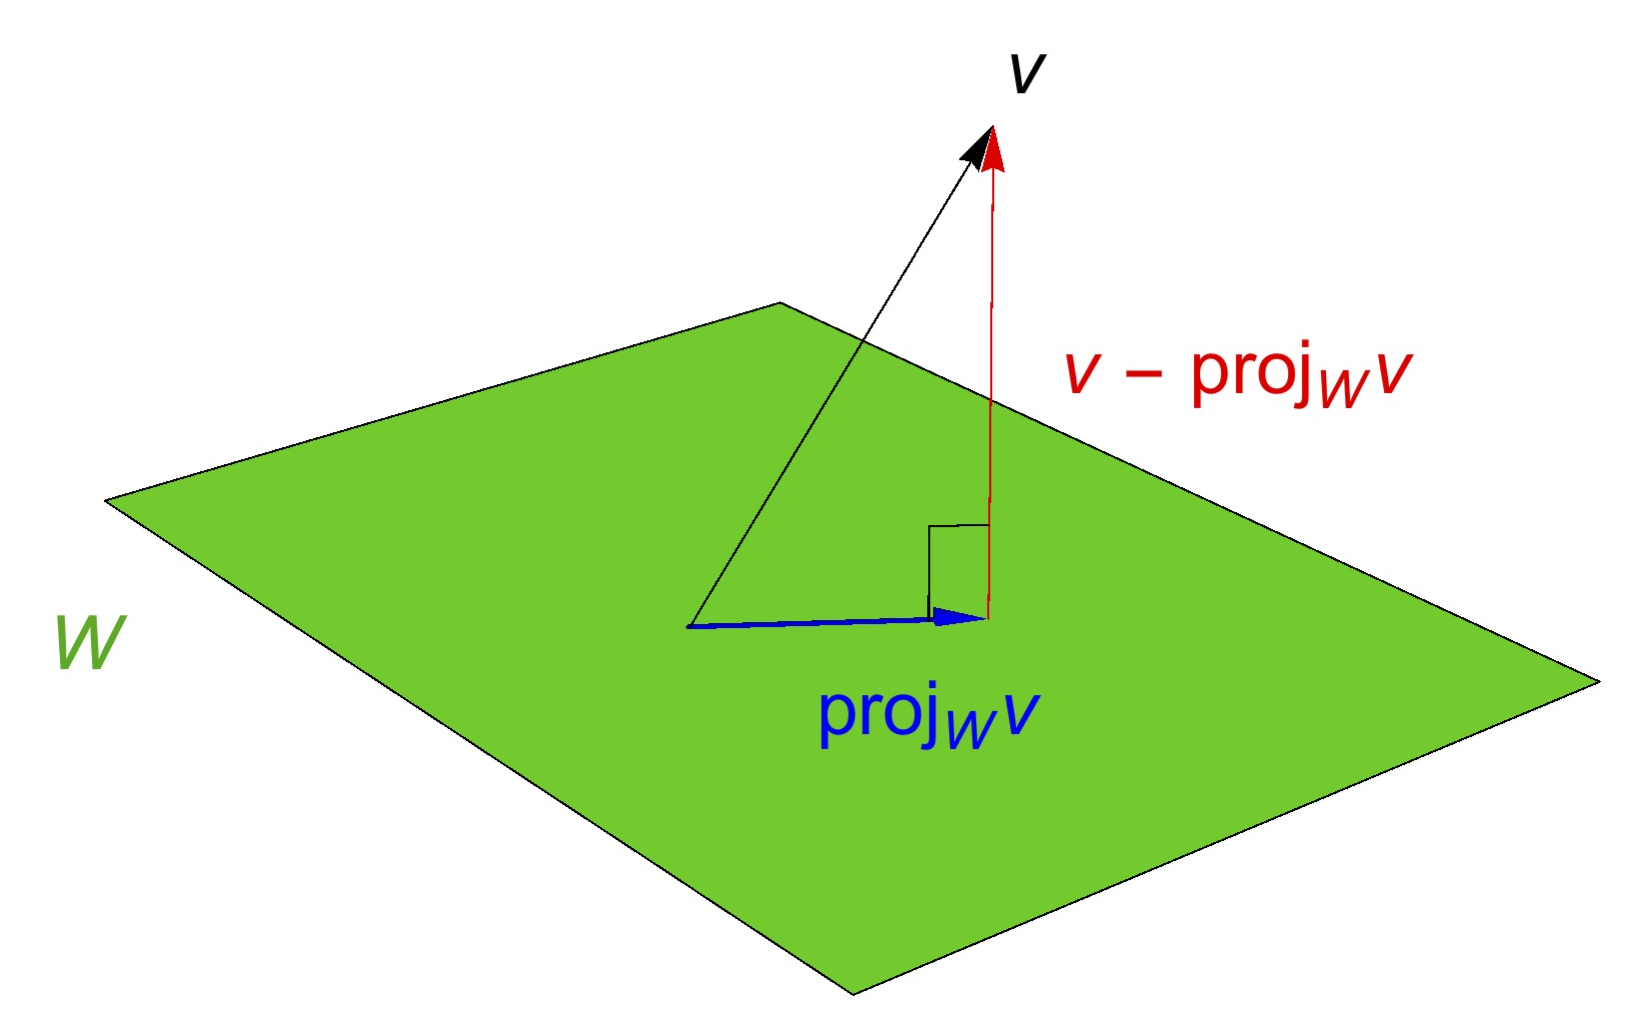
\includegraphics[scale=.2] {img/projW.jpg}~\\[1cm]
\end{center} 
\vglue-1cm
\caption{The orthogonal projection of $\vv$ onto the subspace $W$.}\label{figure:othogproj}
\end{figure}

Now your enquiring mind  may have at least two thoughts at this point. In no particular order, they may be:
\begin{enumerate}

\item {\it Does every subspace have an orthogonal basis?} The formula needs one!\label{goodquestion1}

\item {\it What if I compute this projection with two different orthogonal bases? Surely I'll get  different answers! All the numbers in the sum will be different...}
\end{enumerate}
 
\medskip

We'll answer the second question first -- it doesn't matter\footnote{Amazing fact from linear algebra number 3} which orthogonal basis you use! But not before an example.



\begin{myexample}
Let's look again at $W=\set{(x,y,z,w) \in \R^4 \st x-y-z+w=0}$. We know the three vectors  $\ww_1=(1,1,1,1), \ww_2=(1,-1,1,-1)$ and $ \ww_3=(1,1,-1,-1)$ form an orthogonal basis for $W$.\footnote{Don't worry about how we found these.   We'll discuss that later, in answer to the first question  above.}

Now   $\vv = (1,2,3,5) \notin W$: check it! Let's use the projection formula to find the orthogonal projection of $\vv$ onto $W$, and do a bit of checking.




\begin{mysol}  We begin by calculating:
$$
\frac{\vv\cdot \ww_1}{\|\ww_1\|^2} = \frac{11}{4} 
$$
$$
\frac{\vv\cdot \ww_2}{\|\ww_2\|^2} = \frac{-3}{4} 
$$
$$
\frac{\vv\cdot \ww_3}{\|\ww_3\|^2} = \frac{-5}{4}
$$

and conclude
$$
\proj_W(\vv) = \frac{11}4\ww_1 - \frac34\ww_2 - \frac{5}{4}\ww_3=\frac14(3, 9, 13, 19)
$$
 If you check, you'll see that  $\frac14(3, 9, 13, 19)\in W$: simply show it satsifies $x-y-z+w=0$. 

{\bf N.B. \underbar{You must not rescale this answer!} This is a very, very common error at this stage. Rescaling an orthogonal basis is fine, but the projection is a fixed answer.  }

Moreover, as Figure~\ref{figure:othogproj}, and indeed the properties of $\vv-\proj_W(\vv)$ in $\R^3$ (see Section~\ref{propOrthogProj}  and Figure~\ref{orthoprojonvector})
all suggest,  
$\vv-\proj_W(\vv)=\frac14(1, -1, -1, 1)$ is indeed orthogonal to every vector in $W$: look again at the equation defining $W$: it says $(x,y,z,w) \in W$ iff 
$$ 0=x-y-z+w=(x,y,z,w)\cdot(1, -1, -1, 1)!$$So every vector in $W$ {\it is} orthogonal to $\vv-\proj_W(\vv)$.
\end{mysol} 
\end{myexample}
\standout{This {\it always} happens. And as both Figures \ref{orthoprojonvector} and \ref{figure:othogproj} also suggest, this makes $\proj_W(\vv)$ {\it the \it closest vector in $W$ to $\vv$}. 

Another way to say this is that $\proj_W(\vv)$ is the {\it best approximation to $\vv$ by vectors in $W$}.}

Let's show that this is true:
\begin{theorem}[The Best Approximation Theorem]\index{orthogonal projection}\label{orthogproj}
Let $W$ be a subspace of $\R^n$ and let $\vv \in \R^n$. Then,

\begin{enumerate}[(1)]
\item $\proj_W(\vv) \in W$,
\item $\vv - \proj_W(\vv)$ is orthogonal to every vector in $W$,
\item $\proj_W(\vv)$ is best approximation to $\vv$ by vectors in $W$, and 
\item The vector $\proj_W(\vv)$ is the \underbar{only} vector in $\R^n$ which satisfies (1) and (2).
\end{enumerate} 

\end{theorem}

 

(Property 4 says that the orthogonal
projection is uniqely characterized by the two properties (1) and (2).)


\begin{proof} Part (1) is easy: look at the formula in Definition~\ref{projdef}. The vector $\proj_W(\vv)$ is a linear combination of vectors in the (subspace) $W$ and so must belong to $W$.

For (2), let's think: how {\it could} we  show 
a vector is orthogonal to every vector in $W$? There are infinitely many vectors in (most) subspaces! But that's one thing bases are very good for -- rendering finite  the infinite ! 

So suppose $\{\ww_1, \cdots, \ww_m\}$ is the orthogonal basis for $W$ we used to define the projection. Every $\uu\in W$ is a linear combination of $ \ww_1, \cdots, \ww_m $, \emph{i.e.}, $$\uu =a_1 \ww_1 +\cdots + a_m \ww_m$$ for some scalars $a_, \dots, a_m$. Set $\ww=\proj_W(\vv)$.  So if $(\vv-\proj_W(\vv))\cdot \ww_i=0$  for $1\le i \le m$, then $(\vv-\ww)\cdot \ww_i=0$ so
\begin{align*} 
(\vv-\ww) \cdot \uu &=(\vv-\ww)\cdot (a_1 \ww_1 +\cdots + a_m \ww_m) \\
&=a_1((\vv-\ww)\cdot \ww_1) +\cdots +a_1((\vv-\ww)\cdot \ww_m)\\
&=a_1(0) +\cdots +a_1(0)\\&=0.
\end{align*}
So, it suffices\footnote{Note that we did not use any property of $\{\ww_1, \cdots, \ww_m\}$ except that it spanned $W$, so the same computation shows that a vector is orthogonal to every vector in a subspace $W$ iff it is orthogonal to any {\it spanning set} of $W$.\label{CheckOrthogOnSpan} } to show that $(\vv-\ww)\cdot \ww_i=0$  for $1\le i \le m$.   So we calculate: 
\begin{align*}
 (\vv-\ww)\cdot\ww_i  &=
(\vv - (\frac{\vv\cdot \ww_1}{\Vert \ww_1\Vert^2}\ww_1 + \cdots 
+ 
\frac{\vv\cdot \ww_m}{\Vert \ww_m\Vert^2}\ww_m))\cdot \ww_i \\
 &= \vv \cdot \ww_i - \frac{\vv\cdot \ww_1}{\Vert \ww_1\Vert^2}\ww_1 \cdot \ww_i - \cdots - \frac{\vv\cdot \ww_m}{\Vert \ww_m\Vert^2}\ww_m \cdot \ww_i\\
&= \vv \cdot \ww_i - \frac{\vv\cdot \ww_i}{\Vert \ww_i\Vert^2}\ww_i \cdot \ww_i
\end{align*}

(since all the other dot products between $\ww_i$ and $\ww_j$ are zero);
and this last term gives
$$
 = \vv \cdot \ww_i - \frac{\vv\cdot \ww_i}{\Vert \ww_i\Vert^2}\Vert \ww_i \Vert^2 = 0.
$$
This is true for every $i = 1,2,\cdots, m$ so we conclude that $\vv-\ww$ is orthogonal to every vector in $W$, as required. This shows that (2) is true.


To show that (3) holds, denote, as before $\ww = \proj_W(\vv)$.  To prove this is the closest vector
in $W$ to $\vv$, let $\ww' \in W$ be any other vector in $W$.
Then
$$
\Vert \vv- \ww' \Vert^2 = \Vert (\vv - \ww) + (\ww - \ww') \Vert^2
$$
But since $\vv-\ww$ is orthogonal to every vector in $W$, and $\ww - \ww' \in W$ ($W$ is a subspace and both $\ww$ and $\ww'$ belong to $W$), the two vectors $ \vv - \ww$ and  $\ww - \ww'$
are orthogonal! So by the Pythagorean theorem \ref{eqn:Pythag} on P. \pageref{eqn:Pythag}, we have
$$
\Vert \vv- \ww' \Vert^2 = \Vert (\vv - \ww)\Vert^2 + \Vert(\ww - \ww') \Vert^2 \geq \Vert (\vv - \ww)\Vert^2,
$$
since $0\leq \Vert(\ww - \ww') \Vert^2$  is always true. Thus we've shown (3) is true.

The last part (4) is also straightforward. Now suppose two vectors $\ww,\ww'$ satisfy the properties (1) and (2) above, namely:

\begin{itemize}
\item $\ww, \ww' \in W$
\item $\vv - \ww$ and $\vv-\ww'$ are both orthogonal to every vector in $W$.
\end{itemize}

Then, $\ww- \ww'\in W$ since $W$, being a subspace, is closed under subtraction. But look: $$\ww- \ww'= (\vv-\ww')-(\vv - \ww).$$ Now the sum  -- or difference -- of two vectors which are both orthogonal to every vector in $W$ will again be orthogonal to every vector in $W$.\footnote{I don't know about you, but I'm getting tired of writing `is orthogonal to every vector in $W$', so soon we will save ourslves some bother and give a name to the collection of all vectors orthogonal to every vector in $W$. We'll call it $W^\perp$ --- see Chapter \ref{chapter:20OrthogComp}.} This means that the vector $\ww- \ww'$ is orthogonal to every vector in $W$, including $\ww- \ww'$ itself! But the only vector orthogonal to itself is the zero vector: so $\ww- \ww'=0$, i.e., $\ww= \ww'$.

This  shows that  there is only one vector with the  properties (1) and (2) above, namely $\proj_W(\vv)$.

\end{proof}

Note that  property (3) above of the orthogonal projection is extremely useful, in many areas. It is a huge part of the mathematical foundation for modern signal processing. It is used in almost all quantitative methods for `best' curve fitting for data. We present an example of this in Section~\ref{leastsquares}. 

\medskip

The basic idea it that we have often a `favourite' subspace of vectors $W$ (in a vector space of signals, for example), and another vector that we can't be sure belongs to our subspace, but we only wish to deal with vectors in $W$\kern-2pt, so we project our vector onto $W$ and deal with that instead. 

For example, in a simplified view of signal processing, on your cellphone, for example, when you take a picture and want to send it to a friend, the picture is captured and stored and treated as a vector in a large dimensional space ($\R^n$ for some very large $n$). But instead of sending all the data involved, it will be (orthogonally) projected onto a much smaller subspace -- with an  orthogonal basis peculiar to the protocol being used -- and then only the relatively small number (the dimension of $W$) of Fourier coefficients  will be transmitted. At the other end, your friend will receive the Fourier coefficients, and knowing which  protocol you used, will use the same  orthogonal basis, and rebuild the projection using the the Fourier coefficients, getting an approximation (better or worse, depending on $\dim W$) of the picture you sent.

\medskip

Part (4) above seems innocuous until you recall that Definition~\ref{projdef} {\it looked like} it depended on a choice of orthogonal basis. So what Part (4) is saying is that the {\it apparently} different formulae one gets when using different orthogonal bases to compute the projection all give exactly the same answer!

\section{Finding orthogonal bases: The Gram-Schmidt algorithm}\label{section:Gram-Schmidt}

So far, we've implicitly assumed that every subspace $W$ of $\R^n$ {\it has} an orthogonal basis. Is is true? Yes, and even better, there's a simple algorithm that will take any basis of $W$ as input and output an orthogonal basis of $W$. 

\medskip
 

Suppose  $\set{\uu_1, \cdots, \uu_m }$ is any basis for $W$.  We want to find an orthogonal
basis for $W$.

The geometric idea is quite simple:  start with your first vector $\uu_1$.
Then take $\uu_2 - \proj_{\uu_1}(\uu_2)$ to get something which is
orthogonal to $\uu_1$ but --- crucially --- lies in the span of $\uu_1$
and $\uu_2$.  We then keep subtracting off projections onto the span of the
preceding vectors we obtain and the result is an orthogonal basis for $W$.

\begin{theorem}[Gram-Schmidt Algorithm]\index{Gram-Schmidt algorithm}\label{theorem:GS}
Let $\set{\uu_1, \cdots, \uu_m }$ be {\it any} basis for $U$.  Define
\begin{itemize}
\item $\ww_1 = \uu_1$  and $V_1 = \spn\{\ww_1\}$
\item $\ww_2 = \uu_2 - \proj_{V_1}\uu_2$ and $V_2 = \spn\{\ww_1,\ww_2\}$
\item $\ww_3 = \uu_3 - \proj_{V_2}\uu_3$ and $V_3 = \spn\{\ww_1,\ww_2,\ww_3\}$
\item $\cdots$
\item $\ww_m = \uu_m - \proj_{V_{m-1}}\uu_m$ and $V_m = \spn\{\ww_1,\cdots,\ww_m\}$
\end{itemize}
Then $W = V_m$ and   
$\{\ww_1,\cdots,\ww_m\}$ is an orthogonal basis for $W$.

\medskip
Written out in more detail: define

\begin{itemize}
\item $\ww_1 = \uu_1$,
\item $\ww_2 = \uu_2 - \proj_{\ww_1}\ww_2$,
\item $\ww_3 = \uu_3 - \proj_{\ww_1}\uu_3-\proj_{\ww_2}\uu_3$,
\item $\cdots$
\item $\ww_m = \uu_m - \sum_{i=1}^{m-1}\proj_{\ww_{i}}\uu_m$.
\end{itemize}
Then $\{\ww_1,\cdots,\ww_m\}$ is an orthogonal basis for $U$.

Finally, one could scale each of the  vectors $\ww_i$ by dividing by their norm to produce
an  orthonormal basis for $W$.
\end{theorem}

Notice that at each step, the vectors in the spanning set for $V_i$
are orthogonal, so that means it's easy to calculate the projection onto
$V_k$.  And in fact, $V_k = \spn\{\uu_1 , \cdots, \uu_k\}$; that is, the span of the first
$k$ vectors of the set is the same as the span of the first $k$
vectors of the original spanning set.  

\medskip
Indeed, one could begin with just a {\it spanning} set $\set{\uu_1,\dots, \uu_n}$ for $U$, and apply the Gram-Schmidt Algorithm as above: then the {\it non-zero} vectors in $\{\ww_1,\cdots,\ww_n\}$ would be an orthogonal basis for $U$ - see problem~\ref{prob19.6} in the exercises.

\begin{myexample}\label{example:GS} Let's perform the Gram-Schmidt algorithm on the 
the set
$$\{ (1,0,0,1), (1,1,1,0), (2,1,-1,1)\}
$$
(You can check that this is a basis for the subspace $W=\spn\{ (1,0,0,1), (1,1,1,0), (2,1,-1,1)\}=\set{(x,y,z,w)\in \R^4\st x - y - w = 0}$.\footnote{We saw how to do this at the end of chapter \ref{chapter:15homog}.})


Well, we start with 
$$
\ww_1 = (1,0,0,1)
$$
and then
\begin{align*}
\ww_2 &= \uu_2 - \proj_{\ww_1}\uu_2\\
&= \uu_2 - \frac{\uu_2\cdot \ww_1}{\|\ww_1\|^2}\ww_1 \\
&= (1,1,1,0) - \frac{1}{2}(1,0,0,1) = (\frac12,1,1,-\frac12). 
\end{align*}
(Before going on, it's always a good idea to check that $\ww_1\cdot \ww_2 =0$! It's OK here.)

So in this example, there's just one more step:

\begin{align*}
\ww_3 &= \uu_3 - \frac{\uu_3\cdot \ww_1}{\|\ww_1\|^2}\ww_1 - \frac{\uu_3\cdot \ww_2}{\|\ww_2\|^2}\ww_2\\
&= (2,1,-1,1) - \frac{3}{2} (1,0,0,1) - \frac{\frac12}{\frac52}
(\frac12,1,1,-\frac12) \\
&= (2,1,-1,1) -(\frac32,0,0,\frac32) - (\frac1{10}, \frac15
 , \frac15, -\frac1{10})\\
&= \frac25(1, 2 , -3 , -1).
\end{align*}
Then we can see that $\{\ww_1,\ww_2,\ww_3\}$ is indeed orthogonal -- and it's always a good idea to check this.\footnote{If you can, it's also a very good idea to check that your vectors $\{\ww_1,\ww_2,\ww_3\}$ belong to $W$-- which of course they should! In this case that's easy, as we have a simple description of $W$ -- namely, $W=\set{(x,y,z,w)\in \R^4\st x - y - w = 0}$.}  Also,
by looking at our calculations more carefully, we can see that indeed,
each successive element is in the span of the original vectors. 
The resulting orthogonal basis is
$$
\{ (1,0,0,1), \frac12(1,2,2,-1), \frac25(1,2,-3,-1)\}.
$$  

\begin{remark} We often choose to simplify our calculations when using the formula in Theorem~\ref{theorem:GS} by scaling the 
$\ww_i$ by something convenient to avoid fractions: since 
$$
\{ (1,0,0,1), (1,2,2,-1), (1,2,-3,-1)\}
$$
is just as good an orthogonal set as the one above, and might be
easier to work with if you had to calculate another projection.
\end{remark}

\medskip
Finally, if one really wants  an orthonormal basis, we have to divide each 
of these vectors by their norm.  Since 
$
\Vert (1,0,0,1) \Vert = \sqrt{2}$,  $\Vert  (1,2,2,-1) \Vert =   \sqrt{10}$, and $ \Vert  (1,2,-3,-1) \Vert =   \sqrt{15} $, we obtain the orthonormal basis:
$$
\{ \frac{\sqrt{2}}{2}(1,0,0,1), \frac{\sqrt{10}}{ 10 }(1,2,2,-1), \frac{\sqrt{15}}{15}(1,2,-3,-1)\}.
$$
(Check this!)
\end{myexample}



\begin{myexample}\label{Wagain} Calculate the best approximation to  $\vv = (1,2,3,4)$ in $W$, where
$$
W = \spn\{(1,0,0,1), (1,1,1,0), (2,1,-1,1)\}=\set{(x,y,z,w)\in \R^4\st x - y - w = 0}
$$

Let's use the preceding exercise.  We already know that an
orthogonal basis for $W$ is 
$$
\{  (1,0,0,1),  (1,2,2,-1),  (1,2,-3,-1)\}
$$
(call these $\nn_1$, $\nn_2$ and $\nn_3$, say)
so therefore 
\begin{align*}
\proj_W(\vv) &= \frac{\vv\cdot\nn_1}{\|\nn_1\|^2} \nn_1 +  \frac{\vv\cdot\nn_2}{\|\nn_2\|^2} \nn_2 + \frac{\vv\cdot\nn_3}{\|\nn_3\|^2} \nn_3 \\  
&= \frac{5}{2}  (1,0,0,1) + \frac{7}{10} (1,2,2,-1)  -\frac{8}{15}(1,2,-3,-1)\\
&=  \frac{1}{3}(8,1,3,7).
\end{align*}

If you can, check that your answer actually belongs to $W$: here it's easy since we have a simple description of $W$.\footnote{ If you have the time, you should also check that $(1,2,3,4)-\frac{1}{3}(8,1,3,7)=\frac13(-5,5,0,5)$ is orthogonal to everything in $W$, and it is, since $\frac13(-5,5,0,5).(x,y,z,w)=-\frac53 (x-y-w)=0 $ whenever $(x,y,z,w)\in W$! }
\end{myexample}



\section*{Problems}
\addcontentsline{toc}{section}{Problems}
 
\medskip {\bf Remarks:} 
\begin{enumerate}
\item A question with an asterisk `$ ^\ast$' (or two) indicates a bonus-level question.
 \item You must justify all your responses.
\end{enumerate}
\bigskip

\begin{prob} \label{prob19.1} In each case, find the Fourier coefficients of the vector $\vv$ with respect to the given orthogonal basis $\mathcal B$  of the indicated vector space $W$.
\medskip

\begin{enumerate}[a)]
\item  $\vv=(1,2,3)$, $\mathcal B = \set{(1,0,1),(-1,0,1), (0,1,0) }$, $W=\R^3$.
\medskip
%
\item\sov  $\vv=(1,2,3)$, $\mathcal B = \set{(1, 2 , 3 ),(-5, 4, -1),(1, 1, -1)}$, $W=\R^3$.
\medskip
%
\item  $\vv=(1,2,3)$, $\mathcal B = \set{(1, 0, 1),(-1, 2, 1)}$, $$W=\set{(x,y,z)\in\R^3 \st x+y-z=0}.$$
 
%
\item\sov $\vv=(4,-5,0)$, $\mathcal B = \set{(-1, 0, 5),(10, 13, 2)}$, $$W=\set{(x,y,z)\in\R^3 \st 5x-4y+z=0}.$$
 
%
\item $\vv=(1,1,1,1)$,  $\mathcal B =\set{(1, 0, 1, 1), (0, 1, 0, 0), (0, 0, 1, -1)}$, $$W=\set{(x,y,z, w)\in\R^4 \st x-w=0}.$$
\medskip
%
\item\sov $\vv=(1,0,1,2)$,  $\mathcal B =\set{(1, 0, 1, 1), (0, 1, 0, 0), (0, 0, 1, -1),(1, 0, 0, -1)}$, $W= \R^4$.
\medskip
%
\end{enumerate}

\end{prob} \begin{prob} \label{prob19.2} Find the formula for the orthogonal projection onto the subspaces in parts c), d) \sov and e) above.

\end{prob} \begin{prob} \label{prob19.3} Apply the Gram-Schmidt algorithm  to each of the following linearly independent sets (to obtain an orthogonal set), and check that your resulting set of vectors is orthogonal.
\medskip
\begin{enumerate}[a)]
\item $\set{(1,1,0),(2,0,3)}$
\medskip
%
\item\sov $\set{(1, 0, 0, 1),(0, 1, 0, -1),(0, 0, 1, -1)}$
\medskip
%
\item $\set{(1, 1, 1, 1),(0, 1, 0, 0),(0, 0, 1, -1)}$
\medskip
%
\item\sov $\set{(1, 1, 0),(1, 0, 2),(1, 2, 1)}$
\medskip
%
\end{enumerate}
\end{prob} \begin{prob} \label{prob19.4} Find an orthogonal basis for each of the following subspaces, and check that your basis is orthogonal. (First, find a basis in the standard way, and then apply the Gram-Schmidt algorithm.)
\medskip
\begin{enumerate}[a)]
\item $W=\set{(x,y,z)\in\R^3 \st x+y+z=0}$
\medskip
%
\item\sov 
 $U=\set{(x,y,z, w)\in\R^4 \st x+y-w=0}$\medskip
%
\item $X=\set{(x,y,z, w)\in\R^4 \st x+y-w=0 \, \text{ and } \, z+y=0}$
\medskip
%
\item\sov $V=\ker \bmatrix 1 & 2 & -1 & -1 \\
 2 & 4 & -1 & 3 \\
 -3 & -6 & 1 & -7 \endbmatrix$
\medskip
%
\end{enumerate}

\end{prob} \begin{prob} \label{prob19.5} Find the best approximation to each of the given vectors $\vv$ from the given subspace $W$. \medskip
\begin{enumerate}[a)]
\item  $\vv=(1,1,1)$,  $W=\set{(x,y,z)\in\R^3 \st x+y-z=0}$
\medskip
%
\item\sov $\vv=(1,1,1)$,   $W=\set{(x,y,z)\in\R^3 \st 5x-4y+z=0}$
\medskip
%
\item  $\vv=(1,1,1,2)$,   $W=\set{(x,y,z, w)\in\R^4 \st x-w=0}$
\medskip
%
\end{enumerate}
\end{prob} \begin{prob} \label{prob19.6} State whether each of the following is (always) true,
or is (possibly) false.    
   \smallskip    
\begin{enumerate}[$\bullet$]
\item If you say the statement may be false, you    must give an explicit example.   
\item If you say the statement is true, you must give a clear explanation -   by quoting a theorem presented in class, or by giving a {\it proof valid for every  case}. 
\end{enumerate}
\medskip
\begin{enumerate}[a)]
\item Every orthogonal set is linearly independent.
\medskip
%
\item\sov Every linearly independent set is orthogonal.
\medskip
%
\item When finding the orthogonal projection of a vector $\vv$ onto a subspace $W$, plugging {\it any} basis of $W$ into the formula in Definition~\ref{projdef} will work. 
\medskip
%
\item\sov When finding the orthogonal projection of a vector $\vv$ onto a subspace $W$, once the answer is obtained, it's OK to re-scale the answer to eliminate fractions.
\medskip
%
\item When applying the Gram-Schmidt algorithm to a basis, at each step, it's OK to re-scale the vector obtained to eliminate fractions.
\medskip
% 
\item\sov When finding the orthogonal projection of a vector $\vv$ onto a subspace $W$, using different orthogonal bases of $W$ in the formula in Definition~\ref{projdef} can give different answers.
\medskip
%
\item If $\proj_W(\vv)$ denotes the orthogonal projection of a vector $\vv$ onto a subspace $W$, then $\vv-\proj_W(\vv)$ is always orthogonal to every vector in $W$.
\medskip
%
\item\sov To check that a vector, say $\uu$, is orthogonal to every vector in $W$, it suffices to check that $\uu$ is orthogonal to every vector in {\it any} basis of $W$.
\medskip
%
\item$^{\ast\ast}$ If you apply the the Gram-Schmidt algorithm to a {\it spanning set} $\set{\ww_1, \dots , \ww_m}$ of a subspace $W$, rather than a basis of $W$, and if you obtain a zero vector at step $k$, that means $\ww_k \in \spn\{\ww_1, \dots , \ww_{k-1}\}$.
\medskip
%
\item $^{\ast\ast}$ If you apply the the Gram-Schmidt algorithm to a {\it spanning set} $\set{\ww_1, \dots , \ww_m}$ of a subspace $W$, rather than a basis of $W$, and discard any zero vectors that appear in the process, you will in the end still obtain an orthogonal basis for $W$.
\medskip
%
\end{enumerate}
\end{prob}
  

\chapter{Orthogonal Complements and Applications}
\label{chapter:20OrthogComp}

\section{Orthogonal Complements}
You will recall that one of two important properties of the orthogonal projection $\proj_W(\vv)$ onto a subspace  $W$ was that $\vv-\proj_W(\vv)$ was {\it orthogonal to every vector in that subspace.} This suggests the following definition.



\begin{definition}
Let $U$ be a subspace of $\R^n$.  The \defn{orthogonal complement} of $U$
is the set, denoted $U^\perp$ (pronounced: `$U$-perp') defined by
$$
U^\perp = \set{ \vv \in \R^n \st\uu \cdot \vv = 0 \textrm{\; for all $\uu\in U$}}.
$$
\end{definition}

\begin{myexample}


Let $U = \spn\{ (1,0,3), (0,1,2)\}$. We know that $U$ is the plane through the origin with normal $(1,0,3) \times (0,1,2)=(-3, -2, 1)$. 



So a vector is orthogonal to $U$ iff it is parallel to $(-3, -2, 1)$. Thus,  

$$U^\perp=\spn\{(-3, -2, 1)\}.$$ 
\begin{figure}
\begin{center}
\includegraphics[scale=.5] {img/uperp.jpg}~
\end{center} 
\vglue-.5cm
\caption{The plane $U$ and its orthogonal complement.}\label{figure:Uperp}
\end{figure}

Of course $U^\perp$ is the line through the origin with direction vector $(-3, -2, 1)$.


\end{myexample}


\begin{myexample}
Let $U$ be the subspace of $\R^4$ defined by  $$U=\spn\{(1,-1,0,-1)\} $$ 




Since we already noted that a vector is orthogonal to every vector in a subspace iff it is orthogonal to a basis of the subspace (see the proof of Theorem~\ref{orthogproj}) a vector $(x,y,z,w) \in U^\perp$ iff 
$$(x,y,z,w)\cdot (1,-1,0,-1)= x - y - w=0.$$ That is, in this case, 

$$U^\perp=\set{(x,y,z,w)\in \R^4\st x - y - w = 0}.
$$
You will recognize this subspace as $W$ of Example~\ref{example:GS} from the last two examples in the previous chapter. 
\end{myexample}

What about $W^\perp$ from the example just above?\medskip

\begin{myexample}
Let $W=\set{(x,y,z,w)\in \R^4\st x - y - w = 0}$.

 \medskip

We know that $\vv \in W^\perp$ iff $\vv$ is orthogonal to any basis of $W$. Well, we've lots of those: \emph{e.g.} from Example~\ref{Wagain}: we know that $$ \set{\vv_1=(1,0,0,1), \vv_2=(1,1,1,0), \vv_3=(2,1,-1,1)}$$ is a basis of $W$, so we just need to find  all $\vv$ such that 
\begin{align}\label{eqn:aaa}
\notag \vv_1\cdot \vv&=0\\
\vv_2\cdot \vv&=0\\
\notag \vv_3\cdot \vv&=0.
  \end{align}
We've seen this sort of thing before! Remember Remark~\ref{NullperpRow}? It said, in part, that for a matrix $A$, $\vv\in \Null(A)$ iff $ \vv$ is orthogonal to every row of $A$.

That's what we're staring at above in \eqref{eqn:aaa}. If we set (in block row form)  
$$  A=  \bmatrix \vv_1\\\vv_2 \\\vv_3\endbmatrix$$
So solving the system in (\ref{eqn:aaa}) is equivalent to finding $\Null(A)$! Let's do it:
$$\Null(A)=\Null \bmatrix  1&0&0&1\\1&1&1&0\\2&1&-1&1\endbmatrix =\Null\bmatrix  1 & 0 & 0 & 1 \\
 0 & 1 & 0 & -1 \\
 0 & 0 & 1 & 0 \\\endbmatrix=\set{(-s,s,0,s)\st s\in \R}.$$
So the set of basic solutions -- just one in this case -- namely $\set{(-1,1,0,1)}$ is a basis for $\Null(A)= W^\perp$. But this subspace is our original $U$! 

So $U^\perp=W$ and $W^\perp=U$, or said differently, $(U^\perp)^\perp=U$!  Is this always true?
\end{myexample}

Indeed it is, and more is true as well:

\begin{theorem}[Properties of the orthogonal complement]\index{properties of the orthogonal complement}\label{orthogcompprop}
Let $U$ be a subspace of $\R^n$.  Then:
\begin{enumerate}[(1)]
\item $U^\perp$ is a subspace of $\R^n$
\item $(U^\perp)^\perp = U$
\item $\dim(U) + \dim(U^\perp) = n$.
\end{enumerate}
When two subspaces $U$ and $V$ satisfy $U = V^\perp$ (or equivalently,
$V = U^\perp$) then we say they are \defn{orthogonal complements}.
\end{theorem}

\begin{proof}
(1) We apply the subspace test.  We have
$$
U^\perp = \{ \vv \in \R^n \mid \uu \cdot \vv = 0 \textrm{\; for all $\uu\in U$}.
 \}
$$
(a) Since the zero vector is orthogonal to every vector in $U$ (it's orthogonal
to everything!), $\zero \in U^\perp$. Good.

(b) Suppose $\vv, \ww\in U^\perp$.  That means $\uu \cdot \vv= 0$ and $\uu \cdot \ww =0$.  Is $\vv + \ww \in U^\perp$?  We calculate
$$
\uu \cdot (\vv + \ww) = \uu \cdot \vv + \uu \cdot \ww = 0 + 0 = 0.
$$
OK!

(c) Suppose $\vv \in U^\perp$ and $k\in \R$.  That means $\uu \cdot \vv = 0$.
We calculate
$$
\uu \cdot (k\vv) = k\uu \cdot \vv = k (0) = 0
$$
so indeed $k\vv \in U^\perp$. 

Thus $U^\perp$ is a subspace.


Let's prove (3) next.  Let $\{\uu_1,\ldots, \uu_k\}$ be a basis for $U$.
Create the matrix $A$ whose rows are these vectors (transposed!).
Then the set of all vectors $\vv$ which are orthogonal to $U$
is exactly the set of vectors $\vv$ such that $A\vv = \zero$
(using the argument of the example above).  Hence $U^\perp = \Null(A)$.
By the rank-nullity theorem, 
$$
\dim(\row(A)) + \dim(\Null(A)) = n \Leftrightarrow \dim(U) + \dim(U^\perp) = n.
$$

Finally, to prove (2):  Let $V = U^\perp$; this is a subspace by (1)
and its dimension is $n - \dim(U)$ by (3).   We want to conclude that $U = V^\perp$.  Since every vector in $U$ is indeed orthogonal to every vector in $V$,
it is true that $U \subseteq V^\perp$.  Furthermore, by (3), we have that  $\dim(V^\perp) = n-(n-\dim(U)) = \dim(U)$.  So $U$ is a subspace of $V^\perp$
but has the same dimension as $V^\perp$: it must be all of $V^\perp$.
(This is the theorem about how a subspace that isn't the whole space
must have a strictly smaller dimension.)

\end{proof}

\begin{myprob}
Let $A$ be any matrix.  Show that $\row(A)$ and $\Null(A)$ are orthogonal complements, as are  $\col(A)$ and $\Null(A^T)$.  

\medskip

\begin{mysol}

This is a reprise of our example above, in general.
Suppose $A$ is an $m \times n$ matrix.
Recall that $\Null A=\set{\xx \in \R^n\st A \xx=0}$.
But by definition of the multiplication of matrices, this is
exactly saying that that dot product of each row of $A$ with $\xx$
gives 0.  So $$\Null(A)=\set{\xx \in \R^n \st \xx \text{ is orthogonal to every row of }A}$$ 

Since the rows of $A$ span $\row(A)$, by the footnote \ref{CheckOrthogOnSpan} on page \pageref{CheckOrthogOnSpan},  $\xx \in \Null(A)$ iff $\xx$   is orthogonal to every  vector in $\row(A)$, i.e. $\Null(A)=\row(A)^\perp$, as required.

To see that $\Null(A^T)=\col(A)^\perp$, substitute $A^T$ for $A$ in   $\Null(A)=\row(A)^\perp$ to obtain $\Null(A^T)=\row(A^T)^\perp$ and note that $\col(A)=\row(A^T)$.
\end{mysol}
\end{myprob}





 


\section{Orthogonal projection --- an encore}

Let's use what we know about orthogonal complements to find another way to compute the orthogonal projection. Don't be put off by the first example. It is easy --- we could have done it in high school, but the method we use will be quite different, and will lead to the new way to compute the orthogonal projection.

\bigskip
\begin{myprob}
Find the projection of $\bb = (1,2,3)$ on the subspace $U$
spanned by $\{ (1,1,1)\}$.

\medskip

\begin{mysol}
We're looking for a point $\vv \in U$ such that $\bb-\vv \in U^\perp$.
Think of $U = \col(A)$ where $A = \mat{1\\1\\1}$.
Then $U^\perp = \Null(A^T)$.  

An element of $U$ is the same thing as an element of $\col(A)$, which can
be written as $\vv=Ax$ for some $x$ (in this silly case, $x\in\R$).
To say that $\bb-\vv = \bb-Ax$ is in $U^\perp = \Null(A^T)$
means that 
$$
A^T(\bb-Ax) = 0
$$
or
$$
A^TAx = A^T\bb.
$$
Now $A^TA = (1,1,1)\cdot (1,1,1) = 3$; and $A^T\bb = \mat{1 & 1 & 1}\mat{1\\2\\3} = 6$ so $x = 2$.  Our answer
is 
$$
\proj_U(\bb) = \vv = Ax = \mat{2\\2\\2}
$$
which coincides with our known formula from before:
$$
\proj_{(1,1,1)}((1,2,3)) = \frac{(1,2,3)\cdot (1,1,1)}{\|(1,1,1)\|^2} \mat{1\\1\\1} = \mat{2\\2\\2}.
$$
\end{mysol}\end{myprob}

But we've just found another way to calculate the projection onto
{\it any} subspace of $\R^n$:

\begin{theorem}[Second method to calculate the projection]\index{calculating the projection- second method}
Let $U$ be a subspace of $\R^n$ and let $A$ be a matrix such that
$\col(A) = U$.  Then $\proj_U(\bb)$ is the vector $A\xx$ 
where $\xx$ is any solution to the system
$$
A^TA \xx = A^T \bb.
$$
\end{theorem}

To prove it, just apply the argument in the example above.

Note that because we know that $\proj_U(\bb)$ always exists, the system  
$A^TA \xx = A^T \bb$ will {\it always} be consistent!

\section{Application: Best approximations to solutions of inconsistent systems}

\begin{corollary}[Best Approximation to a Solution]\index{best approximation to a solution of an inconsistent system}
Suppose that $A\xx = \bb$ is inconsistent.  Then the
\defn{best approximation} to a solution of this system is
any vector $\zz$ which solves
$$
A^TA \zz = A^T \bb
$$
That is, such a $\zz$ minimizes $\Vert A\zz - \bb \Vert$.
\end{corollary}

\begin{proof}
Minimizing $\Vert A\zz - \bb \Vert$ over all $\zz \in \R^n$
means finding the closest vector in $\col(A)$ to $\bb$,
since $\col(A)$ is exactly the set of vectors of the form $A\zz$.
So $A\zz$ will be have to be $\proj_{\col A}(\bb)$. This is found exactly as in the theorem above.
\end{proof}

\begin{myprob}
Find the best approximation to a solution for the inconsistent system $A\xx = \bb$ where $\bb = (1,2,1,2)$ and
$$
A = \mat{1 & 0 & 1 \\ 0 & 1 & 0 \\ 0 & 0 & 1\\ 0 & 0 & 0}.
$$
 
\begin{mysol}
Let's apply
the corollary.
We calculate
$$
A^T A = \mat{1 & 0 & 0 & 0\\ 0 & 1 & 0 & 0 \\ 1 & 0 & 1 & 0}
\mat{1 & 0 & 1 \\ 0 & 1 & 0 \\ 0 & 0 & 1\\ 0 & 0 & 0}
=\mat{1 & 0 & 1\\ 0 & 1 & 0 \\ 1 & 0 & 2}
$$
and 
$$
A^T\bb = \mat{1 & 0 & 0 & 0\\ 0 & 1 & 0 & 0 \\ 1 & 0 & 1 & 0}\mat{1\\2\\1\\2} = \mat{1 \\ 2\\ 2}
$$
So we need to solve
$$
\mat{1 & 0 & 1\\ 0 & 1 & 0 \\ 1 & 0 & 2}\mat{x\\y\\z} = \mat{1 \\ 2\\ 2}
$$
which we do by row reducing the augmented matrix
$$
\mat{1 & 0 & 1 &|& 1\\ 0 & 1 & 0 &|& 2\\ 1 & 0 & 2&|& 2}
\sim \cdots \sim
\mat{
1 & 0 & 0 &|& 0\\ 
0 & 1 & 0 &|& 2\\ 
0 & 0 & 1&|& 1}
$$
which has unique solution $(0,2,1)$.  So we claim that
$$
\xx=\mat{0\\2\\1}
$$
gives the best possible approximation to a solution to the
system $A \xx = \bb$; we have
$$
\mat{1 & 0 & 1 \\ 0 & 1 & 0 \\ 0 & 0 & 1\\ 0 & 0 & 0}\mat{0\\2\\1} = \mat{1\\2\\1\\0}
$$
which isn't quite $\bb$ but is fairly close.

To be really convinced this is the best, consider any other $\vv=(x,y,z)$;
then 
$$
A\vv = (x+z, y, z, 0)
$$
so 
$$
\Vert (1,2,1,2) - (x+z, y, z, 0) \Vert^2 = (1-(x+z))^2 + (2-y)^2 + (1-z)^2 + 2^2 
$$
and the answer we found makes the first three terms 0, which clearly gives the 
minimum possible value (4) for the total distance squared.
\end{mysol}\end{myprob}




\section{Application: Least-Squares Best Fitting Line or Curve}\label{leastsquares}

\begin{myprob} Suppose you collect the following data

\begin{center}
\begin{tabular}{|c|c|}
\hline x & y \\
\hline 
-2 & 18 \\
-1 &  8.1 \\
0 & 3.8\\
1 & 3.1\\
2 & 6.1\\
\hline
\end{tabular}
\end{center}
These data points don't exactly lie on a parabola, but you think that's
experimental error; what is the best-fitting quadratic function
through these points?

\medskip

\begin{mysol} 
This doesn't seem to be a linear problem, at first.
Let's rephrase this as a problem in linear algebra!

We want to find a quadratic polynomial
$$
y = a + bx + cx^2
$$
so that when we plug in one of the $x$-values above, we get ``close''
to the $y$ value we measured.

Well, what we're really saying is:  solve for $a,b,c$ (or at least,
try to) in the following linear system:
\begin{align*}
a + b(-2) + c(-2)^2 &= 18\\
a + b(-1) + c(-1)^2 &= 8.1\\
a + b(0) + c(0)^2 &= 3.8\\
a + b(1) + c(1)^2 &= 3.1\\
a+ b(2) + c(2)^2 &= 6.1\,.
\end{align*}
This is the matrix equation
$
A\xx = \bb
$
where 
$$
A = \mat{1 & -2 & 4\\ 1 & -1 & 1\\ 1 & 0 & 0 \\ 1 &  1& 1\\ 1 & 2 & 4}, \qquad \bb = \mat{18\\8.1\\3.8\\3.1\\6.1}.
$$
You can check that this is inconsistent.

So:  we know from above that we should solve instead
$$
A^TA \xx = A^T\bb
$$
where
$$
A^TA = \mat{5&0&10\\0&10&0\\10&0&34}
\qquad
\textrm{and} 
\qquad 
A^T\bb = \mat{39.1\\-28.8\\107.6}
$$
which gives (after a bit of row reduction, and maybe the help of a calculator)
$$
\xx = \mat{3.62\\-2.88\\2.1} = \mat{a\\b\\c}
$$
meaning our quadratic polynomial is
$$
y = (3.62) - (2.88)x + (2.1) x^2.
$$
(You'd need a graphing calculator to see if this is really the best possible fit.)
\end{mysol}\end{myprob}

In what sense was this the ``best answer''?  We minimized the distance between
$A\xx$ and $\bb$.  Recall that if $\xx = (a,b,c)$ then $A\xx$ is
the $y$-values for the points on the curve $a+bx+cx^2$ at the given
$x$-values in the table (or, in the second column of $A$). Call these $(y_{-2}, y_{-1}, y_0, y_1, y_2)$.
 And $\bb$
is the measured values in the table; call these $(y'_{-2}, y'_{-1}, y'_0, y'_1, y'_2)$.
So we've minimized
$$
\Vert A\xx - \bb \Vert^2 = (y_{-2}-y'_{-2})^2 + (y_{-1}-y'_{-1})^2 + (y_0-y'_0)^2 + (y_1-y'_1)^2 + (y_2-y'_2)^2
$$
that is, we've found the  \defn{least squares best fit}: the curve that minimizes the sum of the squares
of the differences in $y$-values.

\standout{This is the de facto standard for fitting curves to experimental data.}

\paragraph{Summary of method:}

\begin{enumerate}
\item Given: data points $(x_i,y_i)$, $i=1,\cdots, n$.
\item Goal: to find the best polynomial of degree $m$ fitting these data points, say
$$
p(x) = a_0 + a_1x+ \cdots + a_mx^m
$$
\item Set $$
A = \mat{1 & x_1 & x_1^2 & \cdots & x_1^m \\
1 & x_2 & x_2^2 & \cdots & x_2^m \\
\ldots & \ldots & \ldots & \ddots & \ldots \\
1 & x_n & x_n^2 & \cdots & x_n^m}
\qquad \textrm{and} \qquad
\bb = \mat{y_1\\y_2 \\ \ldots \\ y_n}
$$
\item Solve $(A^TA) \xx = (A^T\bb)$ for the vector $\xx = (a_0,a_1, \cdots, a_m)$
of coefficients of your best-fitting polynomial.
\end{enumerate}




\section*{Problems}
\addcontentsline{toc}{section}{Problems}
 

\begin{prob} \label{prob20.1} Suppose $U$ is a subspace of $\R^n$.
\medskip

\begin{enumerate}[a)]
\item  Show that $U \cap U^\perp=\set{ \vv\in \R^n \st \vv\in U \text{and } \vv\in U^\perp} =\set{0}$.
\medskip
%
\item\footnote{Hint: look carefully at the seemingly useless equation $\vv= \proj_U(\vv) + \vv-\proj_U(\vv)$. } Show that if $\vv\in \R^n$ is any vector, then there are vectors $\uu\in U$ and $\ww\in U^\perp$ such that $\vv=\uu+\ww$.
\medskip
%
\item Show that if $\vv=\uu+\ww$ and $\vv=\uu'+\ww'$, with $\uu,\uu'\in U$ and $\ww, \ww'\in U^\perp$, then $\uu=\uu'$ and $\ww=\ww'$.
\medskip
%
\end{enumerate}

\end{prob} 

 


%----------------------------------------------------------------------------------------
%	PART V: Determinants, Eigen-everything  and Diagonalization
%----------------------------------------------------------------------------------------

%%%%%%%%%%%%%%%%%%%%%%part.tex%%%%%%%%%%%%%%%%%%%%%%%%%%%%%%%%%%
% 
% sample part title
%
% Use this file as a template for your own input.
%
%%%%%%%%%%%%%%%%%%%%%%%% Springer %%%%%%%%%%%%%%%%%%%%%%%%%%

\begin{partbacktext}
\part{Determinants, Eigen-everything  and Diagonalization}
\noindent We are almost ready to  see one of the most useful and applicable parts of linear algebra: the eigenvalues and eigenvectors of square matrices.  To this end, we need to first develop an important tool: the determinant of a square matrix.
\end{partbacktext}

\chapterimage{Montpellier2.jpg}
% MontpellierPark7301

\renewcommand{\partintrotext}{We are almost ready to  see one of the most useful and applicable parts of linear algebra: the eigenvalues and eigenvectors of square matrices.  To this end, we need to first develop an important tool: the determinant of a square matrix.}

\part{Determinants, Eigen-everything  and Diagonalization}

\chapter{Determinants}
\label{chapter:21Det}
We are about to change gears, and rather dramatically at that.  
Our goal: to uncover the basis for $\R^n$ --- when it exists --- 
that is best or ideally adapted to multiplication by a given $n\times n$ matrix.
This is called a basis of \defn{eigenvectors} (of the matrix),
from the German prefix ``eigen'' meaning ``my own". Eigen-something   means ``my own something", so  eigenvectors of a matrix are the vectors that are special for that matrix. We will see that multiplication of an eigenvector of a matrix  by that matrix gives\footnote{Except in one case: when the {\it eigenvalue} is zero. See section \ref{section:eigen}.} another eigenvector in the same direction.

To get there, though, we first need to master the calculation of
the determinant of a square matrix --- and see why it's such an
interesting number to calculate.\footnote{There is a formula which generalizes the formula we saw in \ref{inverse2by2}  for a $2\times2$ matrix. For the moment, search for `Invertible matrix' and `Adjugate matrix'  for the inverse of an invertible $n \times n$ square matrix you might see in a later course that uses the matrix of cofactors (where
the \defn{cofactors} are the terms $(-1)^{i+j} \det(A_{ij})$ that
appeared in our formulae for the determinant).  As such, it's 
really inefficient for large matrices unless they are quite \defn{sparse}
(meaning: have lots of zeros). 

There's also a formula called {\it Cramer's rule},  for the solution to $A\xx=\bb$ when $A$ is invertible, and that was historically how mathematicians solved systems of
linear equations. In practice one uses Gaussian elimination for any problem involving systems larger that $3 \times 3$, but even for $3 \times 3$ systems,  using  Cramer's rule involves computing {\it four} $3 \times 3$ determinants. You'll see later in this chapter why that's best avoided! 

It's interesting that determinants were discovered long 
before row reduction (in the western world) and determinants were the main route
to results in linear algebra until around 1900. }


\section{The determinant of a square matrix}

Let $A$ be an $n\times n$ matrix.  

When $n=1$, $\det[a] = a$.

When $n=2$, we have previously
discussed the determinant; recall that
$$
\det\left( \mat{a&b\\c&d} \right) = ad-bc
$$
and it's important for two things:
\begin{itemize}
\item  algebraically:  it's the denominator in the formula for the 
inverse of $\mat{a&b\\c&d}$ --- in fact $A$ is invertible if and only
if $\det(A) \neq 0$; and
\item  geometrically: its absolute value is the
area of the parallelogram with sides defined by the vectors
which are the rows of $A$.
\end{itemize}

When $n=3$, we use the same type of formula as for the cross product:
\begin{align*}
\det\mat{a&b&c\\d&e&f\\g&h&i} &= a\det\mat{e&f\\h&i} - b\det\mat{d&f\\g&i} + c\det\mat{d&e\\g&h}\\
&= a(ei-fh) - b(di-fg) +c(dh-eg)
\end{align*}
Note that the end result is again simply  a number, a scalar.  The above
formula is called the \defn{Laplace or cofactor expansion along the first row}.
Its importance includes:
\begin{itemize}
\item in Algebra:  we'll soon show that $\det(A) \neq 0$ if and only if $A$
is invertible (and, although we won't do it this term, there does exist
a formula for the inverse of a matrix with denominator $\det(A)$); and
\item in Geometry:  recall the scalar triple product of vectors $\uu \cdot (\vv \times \ww)$, whose absolute value is the volume of the parallelipiped with sides defined by $\uu, \vv, \ww$.  Note that $\det(A)$ equals
the scalar triple product of the row vectors of $A$.
\end{itemize}

For $n\geq 4$, the formula is recursive, meaning, you need to calculate 
determinants of smaller matrices, which in turn are calculated in terms
of even smaller matrices, until finally the matrices are $2\times 2$
and we can write down the answer.

\begin{definition}
Let $A = (a_{ij})$ (meaning:  the $(i,j)$ entry of $A$ is denoted $a_{ij}$).
Then
$$
\det A = a_{11}\det(A_{11}) - a_{12}\det(A_{12}) + \cdots + (-1)^{1+n}a_{1n}\det(A_{1n})
$$
where $A_{ij}$ is the $(n-1)\times(n-1)$ matrix obtained from $A$ by deleting 
row $i$ and column $j$.
\end{definition}

\begin{myexample}
Let's calculate $\det(A)$ where
$$
A= \mat{
2 & 3 & 4 & 5 \\ 
1 & 0 & 0 & 1\\ 
0 & 1 & 0 & 1\\ 
0 & 0 & 1 & 0}.
$$
Well, the formula says this is
$$
\det A = 2\det\mat{0&0&1\\ 1&0&1\\ 0&1&0} - 3\det\mat{1&0&1\\0&0&1\\0&1&0} +
4\det\mat{1&0&1\\ 0&1&1\\ 0&0&0} - 5\det\mat{1&0&0\\0&1&0\\0&0&1}.
$$
Now to calculate each of the smaller ones, we use the formula again (although
to save time and effort, let's not write down the subdeterminants when
we're just going to multiply the term by 0):
$$
\det\mat{0&0&1\\ 1&0&1\\ 0&1&0} = 0 (\cdot) - 0(\cdot) + 1\det\mat{1&0\\0&1} = 1(1-0) = 1
$$
$$
\det\mat{1&0&1\\0&0&1\\0&1&0} = 1\det\mat{0&1\\1&0} - 0 (\cdot) + 1\det\mat{0&0\\0&1} = 1(0-1) + 1(0-0) = -1
$$
$$
\det\mat{1&0&1\\ 0&1&1\\ 0&0&0} = 1\det\mat{1&1\\0&0} -0 (\cdot) + 1\det\mat{0&1\\0&0} = 0
$$
$$
\det\mat{1&0&0\\0&1&0\\0&0&1} = 1\det\mat{1&0\\0&1} - 0 + 0 = 1
$$
so our final answer is
$$
\det(A) = 2(1)-3(-1) + 4(0) - 5(1) = 0
$$
which is rather interesting.  Do notice that the matrix $A$ is
not invertible: equivalently, $A$ has linearly dependent rows ($R_1=2R_2+3R_3+4R_4$); has
linearly dependent columns ($C_4=C_1+C_2+C_3$); has nontrivial nullspace; has rank less
than $4$, \emph{etc.}).
\end{myexample}

Now, this formula is all well and good, but utterly torturous.  
To calculate the determinant of a $3\times 3$ matrix there are $6=3!$ products of 3 terms, so $2\times 3!$ products
(just counting the hard part, multiplying).  For a $4\times 4$
matrix, it's $3 \times 4\times 6   = 3\times 4!=72$ products that you have to add together.
So for a $10\times 10$ matrix, there are
$$
9\times 10! = 32,659,200  
$$
terms.  For a $100 \times 100$ matrix, you're looking at around $9\times 10^{159}$
terms.  Have fun seeing how long this would take to calculate if
you used the current\footnote{As of (about) 2020: see See {\color{blue}\url{https://en.wikipedia.org/wiki/Fugaku_(supercomputer)}}} fastest computer (Fugaku 415-PFLOPS), which can
do an absolutely astonishing $415.5\times 10^{15}$ calculations per second.
(Hint: there are only about $\pi \times 10^{7}$ seconds in a year....)

Luckily (and remarkably) there are some wonderful shortcuts.

\section{First shortcut: expansion along ANY column or row}

\begin{theorem}[Cofactor expansion along any row or column]\index{calculating the determinant by cofactor expansion along any row or column}
Let $A = (a_{ij})$.  Then the determinant can be  calculated via the \defn{cofactor expansion
along row $i$}, for any $i$:
$$
\det(A) = (-1)^{i+1}a_{i1}\det(A_{i1}) + (-1)^{i+2}a_{i2}\det(A_{i2}) + \cdots + (-1)^{i+n}a_{in}\det(A_{in})
$$
and similarly, the determinant equals the \defn{cofactor expansion along column $j$}, for any $j$:
$$
\det(A) = (-1)^{1+j}a_{1j}\det(A_{1j}) + (-1)^{2+j}a_{2j}\det(A_{2j}) + \cdots + (-1)^{n+j}a_{nj}\det(A_{nj}).
$$
\end{theorem}

\standout{Tip:  the signs you need to use (that is, the factors $(-1)^{i+j}$ in
the cofactor expansion) are given by:
$$
\mat{
+ & - & + & - & + & \cdots \\
- & + & - & + & - & \cdots \\
+ & - & + & - & + & \cdots \\
- & + & - & + & - & \cdots\\
\vdots & \vdots & \vdots & \vdots & \vdots & \ddots}
$$}


\begin{myexample} Calculate
$$\det\mat{2 & 3 & 4\\ 1 & 0 & 3\\ 2 &0 & 4}$$
We could do this on the first row:
$$
\det(A)=2\det\mat{0&3\\0&4} - 3\det\mat{1&3\\2&4}+4\det\mat{1&0\\2&0}
= 2(0) - 3(4-6) +4(0) = 6
$$
or, how about we pick the row or column with the most zeros?  Like
column 2:
$$
\det(A) = -3\det\mat{1&3\\2&4} + 0 - 0 = 6
$$
which is certainly faster.
\end{myexample}

\standout{Moral: choose the row or column with the most zeros to do your cofactor expansion.}

This theorem gives us a couple of immediate consequences:

\begin{proposition}[Quick properties of the determinant]
Let $A$ be an $n\times n$ matrix.
\begin{enumerate}[(1)]
\item If $A$ has a row or column of zeros, then $\det(A) = 0$.
\item $\det(A) = \det(A^T)$.
\end{enumerate}
\end{proposition}

\begin{proof}
(1) Do the cofactor expansion along that row or column; all the terms are zero.

(2) Doing the expansion along row $1$ of $A$ is the same calculation
as doing the expansion along column $1$ of $A^T$, and by the 
theorem you get the same answer. 
\end{proof}


\begin{myexample}
Calculate 
$$
\det \mat{
2 & 2 & 4 & 7 & 6\\
0 & -3 & 7 & 1 & 3\\
0 & 0 & 1 & 12 & -8\\
0 & 0 & 0 & -2 & 21\\
0 & 0 & 0 & 0  & 3}.
$$
This is easy if you do cofactor expansion on the first column:
\begin{align*}
\det A &= 2 \det\mat{-3 & 7 & 1 & 3\\ 0 & 1 & 12 & -8 \\ 0 & 0 & -2 & 21\\ 0 & 0 & 0 & 3} \\
&= 2 (-3) \det\mat{1 & 12 & -8\\ 0 & -2 & 21\\ 0 & 0 & 3}\\
&= 2(-3)(1) \det\mat{-2 & 21 \\ 0 & 3}\\
&= 2(-3)(1)(-2)(3)
\end{align*}
which is simply the product of the diagonal entries!
\end{myexample}

\begin{proposition}[Determinant of triangular matrices]
The determinant of a triangular matrix is  the product of
the diagonal entries.
\end{proposition}

Hmm... notice that every matrix in RREF is triangular, so this
proposition applies.  Thinking about the possibilities, we
conclude:  if $A$ is in RREF then either
\begin{itemize}
\item $A$ has rank $n$ and the determinant is one;
\item $A$ has rank less than $n$ and the determinant is zero.
\end{itemize}
Very nice.  Except:  does this dash our hopes of being
able to calculate the determinant using row reduction?

\section{Second Shortcut:  Using row reduction to calculate the determinant}

It turns out you \stress{can} use row reduction, as long as you
keep track of your steps.  The miracle is that our favourite,
most useful, row reduction step doesn't change the determinant at all!

\begin{theorem}[Effect of row reduction on the determinant]\index{effect of row reduction on the determinant}
Let $A$ be an $n\times n$ matrix and suppose you do an elementary
row operation and the answer is the matrix $B$.  Then:
\begin{enumerate}[(1)]
\item If the row operation was \emph{interchange two rows}
then $\det(B) = -\det(A)$.
\item If the row operation was \emph{multiply a row by $r$}
then $\det(B) = r\det(A)$.
\item If the row operation was \emph{add a multiple of one row to 
another} then $\det(B) = \det(A)$.
\end{enumerate}
\end{theorem}
\begin{remark} The theorem above remains true if `row' is replaced by `column'. 
\end{remark}
\begin{myprob}
Calculate $\det(A)$
where
$$
A = \mat{2 & 1 & 3 & 5 \\ 1 & 2 & 3 & 1\\ 0 & 1 & 2 & 3\\ 0 & 3 & 1 & 4}.
$$

\begin{mysol}
Let's row reduce $A$ and keep track of our operations:
$$
\mat{
2 & 1 & 3 & 5 \\ 
1 & 2 & 3 & 1\\ 
0 & 1 & 2 & 3\\ 
0 & 3 & 1 & 4}
\mt{R_1 \leftrightarrow R_2 \\ \sim}
\mat{
1 & 2 & 3 & 1\\ 
2 & 1 & 3 & 5 \\ 
0 & 1 & 2 & 3\\ 
0 & 3 & 1 & 4}
\mt{ -2R_1+R_2 \\ \sim \\ -3R_3+R_4}
\mat{
1 & 2 & 3 & 1\\ 
0 & -3 & -3 & 3 \\ 
0 & 1 & 2 & 3\\ 
0 & 0 & -5 & -5}
$$
$$
\mt{R_2\leftrightarrow R_3\\ \sim \\ -\frac13R_3\\ -\frac15 R_4}
\mat{ 
1 & 2 & 3 & 1\\ 
0 & 1 & 2 & 3\\ 
0 & 1 & 1 & -1 \\
0 & 0 & 1 & 1}
\mt{-R_2+R_3\\ \sim}
\mat{ 
1 & 2 & 3 & 1\\ 
0 & 1 & 2 & 3\\ 
0 & 0 & -1 & -4 \\
0 & 0 & 1 & 1}
\mt{\sim \\ R_3+R_4}
\mat{
1 & 2 & 3 & 1\\ 
0 & 1 & 2 & 3\\ 
0 & 0 & -1 & -4 \\
0 & 0 & 0 & -3}=R.
$$
OK:  now let's see what our operations did.
The last matrix $R$ has determinant $3$ (by multiplying the
diagonal entries).  The only operations that changed
this value are row interchanges (each at a cost of $-1$) and
scaling rows (each at a cost of the factor you multiplied by). 
So:
$$
\det(R) = (-1)(-\frac13)(-\frac15)(-1)\det(A)
$$
which gives
$$
\det(A) = 15\det(R) = 45.
$$
You can check this by cofactor expansion.
\end{mysol}\end{myprob}

\standout{Point: if you've row reduced and kept track of
your operations, then the determinant can be computed with no extra work.}

\section{Properties of determinants}

\begin{theorem}[Properties of the determinant]\index{properties of the determinant}
Let $A$ and $B$ be $n\times n$ matrices.  Then
\begin{enumerate}[(1)]
\item $\det(rA) = r^n\det(A)$;
\item $\det(AB) = \det(A)\det(B)$;
\item $\det(A) = 0$ if and only if $A$ is not invertible;
\item if $A$ is invertible then $\det(A^{-1}) = \frac{1}{\det(A)}$.
\end{enumerate}
\end{theorem}

\begin{proof}
(1) Multiplying the whole matrix by $r$ means multiplying each of
the $n$ rows of $A$ by $r$; and each of these costs a factor of $r$.
(Geometrically:  the $n$-dimensional volume of a box goes up by a
factor of $r^n$ if you scale every edge by a factor of $r$.)

(2) This takes some effort to prove, but isn't beyond us at all\footnote{ For a reference, see Brescther, \emph{`Linear Algebra with  Applications.'}  }.

(3) We've just seen that row reducing can change the value of 
the determinant by a \stress{nonzero} factor.  So $\det(A) = 0$
if and only if $\det(R) = 0$, where $R$ is the RREF of $A$.
And as we've remarked previously: $\det(R)=0$ if and only if the rank of $A$ is less than $n$, which happens if and only if $A$ is not invertible. 

(4) If $A$ is invertible then $AA^{-1} = I$ so by part (2), we have
$\det(A) \det(A^{-1}) = \det(I) = 1$.
\end{proof} 

%\begin{remark}
%The Vandermonde determinant %shows up in the craziest %places.  Notice,
%for example, that that matrix %is the same one that we use %for least-squares best-fitting %polynomials to a set of data.
%\end{remark} 







\section*{Problems}
\addcontentsline{toc}{section}{Problems}


\medskip {\bf Remarks:} 
\begin{enumerate}
\item A question with an asterisk `$ ^\ast$' (or two) indicates a bonus-level question.
 \item You must justify all your responses.
\end{enumerate}
\bigskip

%\centerline{\bf \underbar{}} 

\begin{prob} \label{prob21.1} Find the determinant of each of the following matrices. In the following, $\lambda$ represents a variable.  Use appropriate row and/or column operations where useful: the definition is the tool of last resort!
\medskip
\begin{enumerate}[a)]
\item 
$\bmatrix
2&-1\\3&0 \endbmatrix $
\medskip
%

\item\sov $\bmatrix 
2&-1&3\\3&0&-5\\1&1&2 \endbmatrix $
\medskip
% 30
\item 
$\bmatrix
1&1&1\\1&2&3\\0&1&1 \endbmatrix $
\medskip
% -1
\item\sov $\bmatrix 3&4&-
1\\1&0&3\\2&5&-4\endbmatrix$\medskip
% -10
\item 
$\bmatrix 0&1&0&0\\
2&0&0&0\\
0&0&3&0\\
0&0&0&4\\
\endbmatrix$ 
\medskip
% -24
\item\sov $\bmatrix \lambda-6&0&0\\0&\lambda&3\\0&4&\lambda+4\endbmatrix $\medskip
%-(\lam -6)(\lam +6)(\lam +2)
 \item $\bmatrix 2&0&0&0&0&0\cr0&1&0&0&0&0\cr0&0&0&1&0&0\cr
0&0&0&0&0&3\cr0&0&1&0&0&0\cr0&0&0&0&3&0\endbmatrix$
\medskip
%
\item\sov $\bmatrix
-\lambda&2&2\\ 2&-\lambda&2\\ 2&2&-\lambda \endbmatrix$
\medskip 
%

\end{enumerate}

\end{prob} \begin{prob} \label{prob21.2} If $\left|\begin{matrix} a&b&c\cr d&e&f\cr g&h&i\end{matrix} \right|=3$,
find 
\medskip
\begin{enumerate}[a)]
 
\item $\left|\begin{matrix}  d&e&f \\ a&b&c\\ g&h&i\end{matrix}\right|$
\medskip
%-3
\item\sov $\left|\begin{matrix}  b&a&c\\ e&d&f\\ h&g&i\end{matrix}\right|$
\medskip
%-3
\item $\left|\begin{matrix}  b&3a&c\\ e&3d&f\\ h&3g&i\end{matrix}\right|$
\medskip
%-9
\item\sov $\left|\begin{matrix}  b&3a&c-4b\\ e&3d&f-4e\\ h&3g&i-4h\end{matrix}\right|$
\medskip
%-9
\item $\left|\begin{matrix} 4g&a&d-2a\cr4h&b&e-2b\cr4i&c&f-2c \end{matrix}\right|$
%12
\medskip

\end{enumerate}

\end{prob} \begin{prob} 
\label{prob21.3} 

 

\begin{enumerate}[a)]


\item If $Q$ is a $3\times 3$ matrix and $\hbox{det}\,Q=2$, find $\det((3Q)^{-1})$.
\medskip
% $\frac{1}{54}
\item\sov If $B$ is a $4\times 4$ matrix and $\hbox{det}(2BB^T)=64$, find $|\det(3B^2B^T)|$.
\medskip
%
\item If $A$ and $B$ are $4\times 4$ matrices with $\det(A)=2$
and $\det(B)=-1$, find $\hbox{det}(3AB^TA^{-2}BA^TB^{-1})$.
\medskip
%
\item\sov Compute the determinant of
$\bmatrix 1&2\cr3&4 \endbmatrix\bmatrix 5&6\cr7&8\endbmatrix 
\bmatrix9&10\cr11&12\endbmatrix\bmatrix 13&14\cr15&16\endbmatrix.$
\medskip
%16
\item  Find all $x$ so that the matrix $\bmatrix 0&x&-
4\cr2&3&-2\cr1&4&1\endbmatrix$ is not invertible.
\medskip
%-5
\end{enumerate}
\end{prob} \begin{prob} \label{prob21.4} State whether each of the following is (always) true,
or is (possibly) false.    
   \smallskip    
\begin{enumerate}[$\bullet$]
\item If you say the statement may be false, you must give an explicit example.   
\item If you say the statement is true, you must give a clear explanation -   by quoting a theorem presented in class, or by giving a {\it proof valid for every  case}. 

\medskip In the following $A$ and $B$ are $n\times n$ matrices (with $n>1$) and $k$ is a scalar.
\end{enumerate}
\medskip
\begin{enumerate}[a)]
\item $\det (AB) = \det(A) \, \det(B)$
\medskip
%
\item\sov $\det (A +B) = \det(A) +\det(B)$
\medskip
%
\item $\det (k A)= k \det(A)$
\medskip
%
\item\sov $\det (k A)= k^n \det(A)$
\medskip
%
\item $\det  A^T = \det(A)$
\medskip
%
\item\sov If $A$ and $B$ are the same except the first row of $A$ is twice the first row of $B$, then $\det(A)=2 \det(B)$
\medskip
%
\item$^{\ast\ast}$ If $A=\bmatrix \cc_1 +\bb_1 & \cc_2 & \cdots& \cc_n \endbmatrix$ is written in block column form, meaning that the first column of $A$ is $\cc_1 +\bb_1$ and $\cc_2, \cc_3, \dots, \cc_n$ are the other columns of $A$, then $\det(A)=   \det \bmatrix \cc_1  & \cc_2 & \cdots& \cc_n \endbmatrix + \det \bmatrix  \bb_1 & \cc_2 & \cdots& \cc_n \endbmatrix $ 
\medskip
%

\end{enumerate}
\end{prob} \begin{prob} \label{prob21.5}
\medskip
\begin{enumerate}[a)]
\item 
\medskip If $A$ is any 2 by  2 matrix, and $\vv_1, \vv_2, \vv_3$ and $\vv_4$ are column vectors in $\R^3$ satisfying $$\bmatrix \vv_1 &\vv_2 \endbmatrix= A  \bmatrix \vv_3 &\vv_4 \endbmatrix,$$show that $\vv_1\times \vv_2 =(\det(A))\, \vv_3\times \vv_4$.
\medskip
%
\item\sov If   $\uu, \vv$ and $\ww$ are  vectors in $\R^3$, use properties of 3 by 3 determinants to show that $$ \uu\cdot \vv\times \ww=  \ww\cdot \uu\times \vv= \vv\cdot \ww\times \uu$$


\item Suppose $B$ is an $1\times n$,  matrix $D$ is an $n\times n$  matrix, $a\in \R$. Show that $\det \bmatrix a&B\\0&D\endbmatrix= a\,\det(D)$. (The matrix is  expressed here in block form.)
\medskip
%
\item$^\ast$\footnote{This is for those of you who know about {\it proofs by induction}.    Search for `Mathematical induction', for example.} Suppose $D$ is an $n\times n$  matrix and $B$ an $m\times n$ matrix. Show that $\det \bmatrix I_m&B\\0&D\endbmatrix= \det(D)$. (The matrix $\bmatrix I_m&0\\0&B\endbmatrix$,  of size $(m+n)\times (m+n)$, is expressed here in block form.)
\medskip
%

\item$^\ast$\footnote{Use the same technique as in the previous part.} Suppose $A$ is an $m\times m$  matrix. Show that $\det \bmatrix A&B\\0&I_n\endbmatrix= \det(A)$. 
\medskip
% 
\item Suppose $A, B$ and $D$ are respectively of sizes $m\times m$,   $m \times n$ and $n \times n$. Noting that $ \bmatrix A&B\\0&D\endbmatrix =\bmatrix I_m&0\\0&D\endbmatrix\bmatrix A&B\\0&I_n\endbmatrix$, show that $\det \bmatrix A&B\\0&D\endbmatrix= \det(A) \det(D)$. 
\medskip
%
\item\sov Suppose $A, B, C$ and $D$ are respectively of sizes $m\times m$,   $m \times n$, $n \times m$ and $n \times n$. Suppose that $D$ is invertible. Noting that $ \bmatrix A&B\\C&D\endbmatrix \bmatrix I_m&0\\-D^{-1}C&I_n\endbmatrix  =\bmatrix A-BD^{-1}C&B\\0&D\endbmatrix$, show that $\det \bmatrix A&B\\C&D\endbmatrix= \det (A-BD^{-1}C) \det(D)$.
\medskip
% 
\item Suppose $A, B, C$ and $D$ are $n\times n$ matrices with $D$ invertible and  $CD=DC$. Let $E=\bmatrix A&B\\C&D\endbmatrix$,  an $(2n)\times (2n)$ matrix, expressed here in block form. Use the last part and properties of the determinant to show that $\det \bmatrix A&B\\C&D\endbmatrix= \det (AD-BC)$.  \medskip
%
\item$^{\ast\ast\ast}$ \footnote{This is for those of you who know about {\it continuity}, and the fact that invertible $n\times n$ matrices are {\it dense} in all $n\times n$ matrices. Search for `Invertible\_matrix'. There is another proof of this identity that doesn't use the density argument, by J.R. Silvester, in {\it Determinants of block matrices}, Math. Gaz., 84(501) (2000), pp. 460-467.} Suppose $A, B, C$ and $D$ are $n\times n$ matrices with  $CD=DC$. Show that $\det \bmatrix A&B\\C&D\endbmatrix= \det (AD-BC)$.  \medskip
%
\item$^{\ast\ast}$ Suppose $A$ is a 3 by 3 matrix that satisfies $AA^T=I_3$. \medskip

\begin{enumerate}[i)]
\item Show that $A^TA=I_3$ as well.
\medskip
%
\item Suppose $\set{\ee_1, \ee_2, \ee_3}$ is the standard (orthogonal and orthonormal) ordered basis of $\R^3$. Using the fact that the dot product $\vv\cdot \ww$ is equal to the matrix product $\vv^T \ww$ (writing vectors as $3 \times 1 $ matrices), show that $\set{A\ee_1, A\ee_2, A\ee_3}$ is also an orthogonal set, which is indeed {\it orthonormal.}
\medskip
%
\item If $\uu$ and $\vv$ are any vectors in $\R^3$, use the Expansion theorem \ref{expansion} to show that $$\uu \times \vv=  \displaystyle \sum_{i=1}^3 (\uu \times \vv)\cdot \ee_i$$ and $$A\uu \times A\vv= \dsize\sum_{i=1}^3 (A\uu \times A\vv)\cdot A\ee_i.$$
\medskip
%
\item Recalling the definition of the 3 by 3 determinant, show that $$(\uu \times \vv)\cdot \ee_i=\det\bmatrix \uu&\vv&\ee_i\endbmatrix$$ and   $$(A\uu \times A\vv)\cdot A\ee_i=\det\bmatrix A\uu&A\vv&A\ee_i\endbmatrix,$$ where the matrices $\bmatrix \uu&\vv&\ee_i\endbmatrix$ and $ \bmatrix A\uu&A\vv&A\ee_i\endbmatrix$ on the right have been written in block column form.
\medskip
%
\item Recalling what you know about block multiplication, and properties of determinants, show that $$\det\bmatrix A\uu&A\vv&A\ee_i\endbmatrix=\det(A)\det \bmatrix  \uu& \vv& \ee_i\endbmatrix.$$
\medskip
%
\item Now prove that  for any vectors $\uu, \vv \in \R^3$, (when $AA^T=I_3$) $$A\uu \times A\vv =\det(A) \, (\uu\times \vv)$$
\medskip
%
\item Give an example of a matrix $A$, which does not satisfy $AA^T=I_3$ and two vectors $\uu,\vv \in \R^3$ for which $A\uu \times A\vv \not=\det(A) \, (\uu\times \vv)$
\medskip
%

\end{enumerate}

\end{enumerate}
\end{prob}


\chapter{Eigenvalues and Eigenvectors}
% of a (square) matrix}
\label{chapter:22Eigen}
This chapter and the next are amongst two of the most useful and applicable parts of all of linear algebra! Get ready for a great ride.

\section{Eigenvalues and Eigenvectors of a (square) matrix}
\begin{definition}\label{section:eigen}
Let $A$ be an $n\times n$ matrix.  
If $\lambda\in \R$ is a scalar and $\xx \in \R^n$ is a \stress{nonzero} vector 
such that
$$
A \xx = \lambda \xx
$$
then $\xx$ is called an \defn{eigenvector of $A$} and $\lambda$ is its
corresponding \defn{eigenvalue}.
\end{definition}

\begin{myexample}
Let $A = \mat{3 & -1 \\ -2 & 2}$.  Then:
\begin{itemize}
\item $1$ is an eigenvalue and $(1,2)$ is an eigenvector corresponding to $\lambda = 1$ because $$A\mat{1\\2} = \mat{1\\2}=1\mat{1\\2}.$$
\item $4$ is an eigenvalue and $(-1,1)$ is an eigenvector corresponding to $\lambda = 4$ because $$A\mat{-1\\1} = \mat{-4\\4}.$$
\end{itemize}
Note that $(10,20)$ and $(17,-17)$ are also eigenvectors of $A$; but
they are just multiples of what we already found.
\end{myexample}

\begin{myexample}
Let $A = \mat{1 & 1\\ 2 & 2}$.  Then 
$0$ is an eigenvalue, and $(1,-1)$ is a corresponding eigenvector,
since $A\mat{1\\-1} = \zero = 0\mat{1\\-1}$.
\end{myexample}

\standout{The matrix $A$ can have $0$ as an \stress{eigenvalue}
but the vector $\zero$ is NEVER an \stress{eigenvector}.}

The essential application:  
suppose you can find a basis  $\{ \xx_1,\cdots,\xx_n\}$  for $\R^n$ consisting of
eigenvectors of $A$, with corresponding eigenvalues $\lambda_1,\cdots, \lambda_n$.
Then if $\vv = a_1 \xx_1 + \cdots + a_n \xx_n$
then
\begin{align*}
A\vv &= A(a_1 \xx_1 + \cdots + a_n \xx_n)\\
 &= A(a_1 \xx_1) + \cdots + A( a_n \xx_n)\\
&= a_1 A\xx_1 + \cdots + a_n A\xx_n\\
&= a_1\lambda_1 \xx_1 + \cdots + a_n\lambda_n \xx_n\\
&= \lambda_1a_1\xx_n + \cdots + \lambda_na_n\xx_n.
\end{align*}
So although the answer won't be a scalar multiple of $\vv$ (since the
$\lambda_i$ may be different), the point
is:  given a vector $\vv$ in coordinates relative to an eigenbasis, calculating
$A\vv$ doesn't require us to multiply matrices at all --- we just have to
scale each of the coordinates (coefficients) by the appropriate $\lambda_i$.

(For those of you thinking in terms of computarional complexity:  this means
going from $O(n^2)$ to $O(n)$ --- fairly significant!)


\section{Finding eigenvalues of $A$}

Since both $\lambda$ and $\xx$ are unknown, the equation $A\xx = \lambda \xx$ is
in fact nonlinear.  As we've seen previously, however, we can sometimes 
turn nonlinear equations into linear ones by focussing on solving for
one set of variables at a time.

The \stress{key} is the following chain of equalities, which
turns $A\xx = \lambda \xx$ into the equation $( A- \lambda I) \xx = \zero$:
\begin{align*}
& A\xx = \lambda \xx \\
\iff & A\xx = \lambda I \xx\\
\iff & A\xx - \lambda I \xx =\zero  \\
\iff & (A-\lambda I )\xx=\zero  
\end{align*}
This point of view is the key to letting us solve the problem using
our methods from before, as follows.

First think of $\lambda$ as being a fixed, known quantity.  Then
this equation is a homogeneous system of linear equations, and
any \stress{nontrivial} solution is an eigenvector of $A$.  In
other words:  
\begin{itemize}
\item if this system has a unique solution, then there
are no eigenvectors corresponding to $\lambda$, which means
$\lambda$ is not an eigenvalue.
\item if this system has infinitely many solutions, then any nontrivial
one of these is an eigenvector, and so $\lambda$ is an eigenvalue.
\end{itemize}
We can rephrase this as follows, by remembering that when $A$ is
a square matrix, having infinitely many solutions to a linear
system is the same as being not invertible:

\standout{The number $\lambda$ is an eigenvalue of $A$ if 
and only if the matrix $A-\lambda I $ is NOT invertible.}

We could use many different methods to check if the matrix is not
invertible, but since the matrix has a variable in it (namely,
$\lambda$) the nicest one is the determinant condition:

\standout{The number $\lambda$ is an eigenvalue of $A$ if 
and only if $\det( A- \lambda I)=0$.}

\begin{definition}\label{charpoly}
The polynomial $\det( A- \lambda I)$ is called the \defn{characteristic
polynomial} of $A$\footnote{Some authors prefer $\det( \lambda I -A)$, but for our computational purposes, using $\det( A- \lambda I)$ is less prone to error, and gives exactly the same answer, up to a sign.}.
\end{definition}

\begin{myprob}
Find all the eigenvalues of $A = \mat{1 & 3 \\ 3 & 1}$.

\begin{mysol}
We need to find all values of $\lambda$ so that $A-\lambda I $ is
not invertible.  Begin by writing down $A-\lambda I $:
$$
A-\lambda I = \mat{1 & 3 \\ 3 & 1} -\mat{\lambda & 0 \\ 0 & \lambda}
= \mat{  1-\lambda & 3\\ 3 &   1-\lambda}
$$
(watch those negative signs on the two $\lambda$s!).

We calculate the characteristic polynomial:
$$
\det(A-\lambda I) = (1-\lambda)(1-\lambda) - 9  = \lambda^2 -2\lambda -8
 = (\lambda - 4)(\lambda + 2),
$$
and deduce that this is zero iff $\lambda$ is either $4$ or $-2$.
Hence, the eigenvalues of $A$ are $4$ and $-2$.  

To check, let's write down $ A-4I$ and $A+2I$ and make sure they are
in fact non-invertible:
$$
A-4I = \mat{-3&3\\3&-3}\sim \mat{1&-1\\0&0}, \qquad A+2I = \mat{3&3\\3&3}\sim \mat{1&1\\0&0}
$$
Good! Because both these matrices are not invertible, it's now clear that $4$ and $-2$ are eigenvalues of $A$. To
see that these are ALL the eigenvalues of $A$, note that $\det(A-\lambda I)$
is a quadratic polynomial and so has {\it at most} two roots.

 
\end{mysol}\end{myprob}
 
 Key for calculations:
The eigenvalues of $A$ are the roots of the characteristic polynomial 
$\det( A-\lambda I )$.  

\begin{definition}\label{def:algmult}
The multiplicity of $\lambda$ as a root of the characteristic polynomial
is called its \emph{algebraic multiplicity}.
\end{definition}
 
\begin{myexample}
The characteristic polynomial of $\mat{16& 2 & 17 \\ 0 & -43 & 14\\ 0 & 0 & 16}$
is $-(\lambda - 16)^2(\lambda + 43)$. (Check!)  Hence the eigenvalues of this
matrix are $\lambda = -43$ (with algebraic multiplicity $1$) and
$\lambda = 16$ (with algebraic multiplicity $2$).
\end{myexample}

\section{Finding the eigenvectors of $A$}

Suppose now that you have found some eigenvalues of the
matrix $A$.  To find the eigenvectors of $A$ associated
to that eigenvalue, recall that they are all the nontrivial
solutions $\xx$ of
$$
( A- \lambda I) \xx = \zero.
$$
In other words: the eigenvectors of $A$ asssociated to $\lambda$
are the nonzero vectors in $\ker( A- \lambda I)= \Null( A- \lambda I)$.

\begin{definition}
Let $\lambda$ be an eigenvalue of $A$.  Then the subspace
\begin{align*}
E_\lambda &= \Null(A- \lambda I)\\
&= \{ \xx \in \R^n \mid (A- \lambda I)\xx = \zero \} \\
& = \{ \xx \in \R^n \mid A\xx = \lambda \xx \}
\end{align*}
is called the $\lambda$-eigenspace of $A$.
Its {\it nonzero} elements are the eigenvectors of $A$ corresponding
to the eigenvalue $\lambda$.
\end{definition}

So rather than ask: ``What are the eigenvectors of $A$?'' it's
simpler to ask: ``What is a basis for each eigenspace of $A$?''.

\begin{myprob} Find a basis for each eigenspace of 
$$
A = \mat{1 & 3 \\ 3 & 1}
$$
(recalling that its eigenvalues were $4$ and $-2$).

\begin{mysol}
For the eigenvalue $\lambda = 4$:
$$
A-\lambda I = A-4I = \mat{-3&3\\3&-3} \sim \mat{1 & -1\\0&0}
$$
so the general solution to $(A-4I)\xx = \zero$ is
$$
E_4 = \Null(A-4I) = \{(r,r) \mid r\in\R\}
$$
and a basis for $E_4$ is
$$
\{ (1,1) \}.
$$
(Notice that with $\xx = (1,1)$, $A\xx = 4\xx$, as required.)


For the eigenvalue $\lambda = -2$:
$$
 A-\lambda I = A+2I = \mat{3&3\\3&3} \sim \mat{1&1\\0&0}
$$
so the general solution to $(A-2I)\xx = \zero$ is
$$
E_{-2} = \Null(A+2I) = \{(-r,r) \mid r\in\R\}
$$
and a basis for $E_{-2}$ is
$$
\{ (-1,1) \}.
$$
(Notice that with $\xx = (-1,1)$, $A\xx = -2\xx$, as required.)
\end{mysol}\end{myprob}

The dimension of the eigenspace associated to the eigenvalue $\lambda$ is another important number we want to keep track of.

\begin{definition}
The dimension of the eigenspace $E_\lambda$ is called the
\defn{geometric multiplicity} of $\lambda$.
\end{definition}

\section{Towards an eigenvector basis of $\R^n$}

We notice that so far, the eigenvectors we are getting for 
different eigenvalues are linearly independent.  That's not
too hard to see for two vectors, but takes a little more work for more.\footnote{The best way is to use {\it Induction}.}  

\begin{theorem}[Independence of Eigenvectors --- Distinct Eigenvalues]
Let $A$ be an $n\times n$ matrix.  Then any set consisting
of eigenvectors of $A$ corresponding to distinct eigenvalues
is linearly independent.
\end{theorem}

Let's put this together:
\begin{itemize}
\item The characteristic polynomial of an $n\times n$ matrix $A$ is
a polynomial of degree $n$, so it has at most $n$ distinct roots.
\item Each root of the characteristic polynomial is an eigenvalue of $A$.
\item Each eigenvalue of $A$ gives an eigenspace of dimension at least $1$.
\item So IF the characteristic polynomial has exactly $n$ distinct
roots, then we can choose one eigenvector from each eigenspace and
thus produce a basis of $\R^n$ consisting entirely of eigenvectors
of $A$.
\end{itemize}

\begin{definition}\label{diagble}
The $n\times n$ matrix $A$ is said to be \defn{diagonalizable over the reals} if there
is a basis of $\R^n$ consisting entirely of eigenvectors of $A$.
\end{definition}

(Why ``diagonalizable'', you say?  We'll come back to this in a bit.)

\begin{fac}If an $n\times n$ matrix $A$ has $n$ distinct
{\it real} eigenvalues then $A$ is diagonalizable.\end{fac}

\medskip
Can a matrix  ever fail to be diagonalizable?
 
\section{Problematic cases: Case I (not enough real roots)}

\begin{myexample} What are the eigenvalues of 
$$
A = \mat{\cos \theta & \sin \theta \\ -\sin \theta & \cos \theta}?
$$
Well:  the characteristic polynomial is
\begin{align*}
\det( A-\lambda I )& = \det\mat{ \cos \theta-\lambda  & \sin \theta \\ -\sin \theta & cos \theta-\lambda}\\
& = (\lambda-\cos \theta)^2 + \sin^2\theta\\&= \lambda^2 -2\cos(\theta)\lambda + \cos^2\theta + \sin^2\theta\\
&= \lambda^2 -2\cos(\theta)\lambda +1.
\end{align*}
Its roots, using the quadratic formula, are:
$$
\lambda = \frac{1}{2}\left(2\cos\theta \pm \sqrt{4\cos^2\theta - 4}\right)
= \cos\theta \pm \sqrt{-\sin^2\theta} = \cos\theta \pm i \sin\theta
$$
which are complex numbers unless $\sin \theta=0$, \emph{i.e.}, $\theta=0$ or $\pi$.  

If we were to calculate the eigenvectors associated to these
eigenvalues for $\theta\not=0, \pi$, they would have complex coordinates --- meaning
they aren't in $\R^2$, but in $\C^2$.  That's fine for 
certain types of applications but not for others; mathematically
we usually work over $\C$ (because the fundamental theorem
of algebra tells us that's where all the roots will lie)\footnote{\label{diagC}Indeed, if we allow complex scalars, and so complex eigenvalues and complex eigenvectors in $\C^2$, $\C^2$ does have a basis of eigenvectors of the matrix $A$. In this case, we say $A$ is {\it diagonalizable over $\C$.}}.

If you happen to know that  $
A = \mat{\cos \theta & \sin \theta \\ -\sin \theta & \cos \theta}
$ is a rotation matrix, it's pretty clear why (when $\theta\not=0, \pi$) there are no real values of $\lambda$ for which rotation of a vector $\xx \in \R^2$ by $\theta$, namely $A\xx$,  will result in a real multiple $\lambda \xx$ of $\xx$!
\end{myexample}

\standout{Moral:  it can happen that some eigenvalues are
complex numbers.  In this case, you will not get an eigenvector
basis of $\R^n$; $A$ is not diagonalizable over $\R$. }


\section{Problematic cases: Case II (not ``enough'' eigenvectors)}

By definition, if $\lambda$ is an eigenvalue then $\dim(E_\lambda) \geq 1$.
But it $\lambda$ is a repeated root of the characteristic equation,
say of multiplicity $k$, then we'd really need $\dim(E_\lambda) = k$,
and that doesn't always happen:

\begin{myprob} Find the eigenvalues of $A = \mat{3 & 1\\ 0 & 3}$ and a
basis for each eigenspace.

\begin{mysol} The characteristic polynomial is $(\lambda -3)^2$ so
the only eigenvalue is $3$ (with algebraic multiplicity $2$).
But  $\rnk(A- 3I) = 1$ so $\dim E_2 = \dim \Null(A- 3I) = 2-1=1$.
That is, we only got a 1-dimensional subspace of eigenvectors,
so it's impossible to find an eigenvector basis of $\R^n$.
$A$ is not diagonalizable over the reals (or even over $\C$). % - see the footnote on P. \pageref{diagC}).
\end{mysol}\end{myprob}

\standout{If the characteristic polynomial has a
repeated root, then it \stress{can happen} that we do not have enough
linearly independent eigenvectors of $A$ to form a basis.}

\begin{myexample} Consider 
$$
A = \mat{3 & 2 & 4\\ 2& 0 & 2\\ 4 & 2 & 3}
$$
Find all eigenvalues and a basis for each eigenspace and decide
if $A$ is diagonalizable.\footnote{This example is done in detail in Section~\ref{section:diag}.  }

You'll find that $A$ is in fact diagonalizable, even though
its characteristic polynomial has a repeated root.  
\end{myexample}


These examples illustrate a fundamental fact.

\begin{theorem}[Limits of geometric multiplicity]\index{limits of geometric multiplicity}\label{thm:limitsmult}
Let $\lambda$ be an eigenvalue of $A$.  Then 
the geometric multiplicity of $\lambda$ is at least $1$, and
at most equal to the algebraic multiplicity of $\lambda$.  That
is,
$$
1 \leq \dim E_\lambda \leq \textrm{algebraic multiplicity of $\lambda$}
$$
\end{theorem}

Note that the first inequality  follows directly from the definition:  $\lambda$
being an eigenvalue implies that the eigenspace is nonzero (and so
must have dimension at least $1$).  (Showing the other inequality is
more work and we will not prove it here.)


\section*{Problems}
\addcontentsline{toc}{section}{Problems}


\medskip {\bf Remarks:} 
\begin{enumerate}
\item A question with an asterisk `$ ^\ast$' (or two) indicates a bonus-level question.
 \item You must justify all your responses.
\end{enumerate}
\bigskip

%\centerline{\bf \underbar{}} 

\begin{prob} \label{prob22.1} Find the eigenvalues of the following matrices. 
\medskip
\begin{enumerate}[a)]
 
\item $\bmatrix
2&1\\3&0 \endbmatrix $
\medskip
%{3, -1};{{1, 1}, {-1, 3}}
\item\sov  $\bmatrix 
1&1&1\\1&1&-1\\1&1&2 \endbmatrix $
\medskip
%{2, 2, 0};{{1, -1, 2},  {-1, 1, 0}}
\item $\bmatrix 
1&0&1\\0&1&-1\\1&1&2 \endbmatrix $
\medskip
%{2, 1, 1};{{1, -1, 1}, {-1, 1, 0}, {0, 0, 0}}

\item\sov $\bmatrix 
1&0&1\\0&1&0\\1&1&1 \endbmatrix $
\medskip
%{2, 1, 0};{{1, 0, 1}, {-1, 1, 0}, {-1, 0, 1}}
\item $\bmatrix 
1&0&1\\0&1&0\\2&1&2 \endbmatrix $
\medskip
%{3, 1, 0};{{1, 0, 2}, {-1, 2, 0}, {-1, 0, 1}}
\item\sov $\bmatrix 
2&1&0\\0&2&1\\0&0&2 \endbmatrix $
\medskip
% 2:{{1, 0, 0}}
\item $\bmatrix 
1&0&1\\0&1&-1\\1&1&2 \endbmatrix $\medskip
%{2, 1, 1};{{1, -1, 1}, {-1, 1, 0}}
\item\sov $\bmatrix 
2&1&0\\0&2&0\\0&0&2 \endbmatrix $
\medskip
% 2:{{1, 0, 0}}
\item $\bmatrix 
3&1&0\\0&3&0\\0&0&2 \endbmatrix $
\medskip
%{3,3,2}:{{1, 0, 0}, {0, 0, 0}, {0, 0, 1} 
 
\end{enumerate}

\end{prob} \begin{prob} \label{prob22.2} For each of the matrices  in the previous question, find a basis for each eigenspace. (Solutions to parts b, d, f and h are available.)\medskip
% 

\end{prob}
\chapter{Diagonalizability}
\label{chapter:23Diag}
 


In the previous chapter, we defined the eigenvalues and eigenvectors of a square matrix $A$.  To each eigenvalue we associate its \emph{algebraic multiplicity}, which is its multiplicity as a root of the characteristic polynomial $\det(A-\lambda I)$ of $A$.  We also associate to each eigenvalue its \emph{geometric multiplicity}, which is the dimension of the associated eigenspace $E_\lambda$.  The key result (Theorem~\ref{thm:limitsmult}) is that for each eigenvalue $\lambda$ of $A$, we have
$$
1 \leq \text{geometric multiplicity of $\lambda$} \leq
\text{algebraic multiplicity of $\lambda$}.
$$
In particular, the dimension of the eigenspace $E_\lambda$ can \emph{never} be larger than the algebraic multiplicity of $\lambda$.
 
\section{About diagonalizability}\label{section:diag}

Recall Defintion \ref{diagble}:
The $n\times n$ matrix $A$ is said to be \defn{diagonalizable over the reals} if there
is a basis of $\R^n$ consisting entirely of eigenvectors of $A$.
 

We saw last time that if $A$ has $n$ distinct real eigenvalues,
then $A$ is diagonalizable.  But $A$ can be diagonalizable even
if it has repeated eigenvalues (it's just not {\it guaranteed} to work):

\begin{myprob} Consider 
$$
A = \mat{3 & 2 & 4\\ 2& 0 & 2\\ 4 & 2 & 3}
$$
Find all eigenvalues and a basis for each eigenspace and decide
if $A$ is diagonalizable.

\begin{mysol}  We need to calculate the eigenvalues of $A$ first.  So
we begin by computing the characteristic polynomial:
$$
\det( A-\lambda I) = 
\det \mat{
3-\lambda & 2      & 4 \\ 
2          & -\lambda & 2 \\ 
4          & 2      &  3-\lambda }
$$
Although we could compute this directly, it's easier with
some zeros, so try the row operation $-2 R_2  + R_3 \to R_3$, which doesn't change
the value of the determinant:
$$
= \det \mat{
3-\lambda & 2      & 4 \\ 
2          & -\lambda & 2 \\ 
0          & 2+2 \lambda \,     &  - 1 -\lambda}
$$
and now we notice that the $(3,2)$ entry is exactly $-2$ times the
$(3,3)$ entry.  So, remembering that the determinant of a
matrix is the same as that of its transpose, we can perform the column operation
$2C_3+C_2\to C_2$ and this won't change the determinant either:
$$
=  \det \mat{
3-\lambda & 10      & 4 \\ 
2          & 4-\lambda & 2 \\ 
0          & 0 \,     &  - 1 -\lambda}
$$
and now if we do the cofactor expansion on the third row, we'll
get a partially factored answer:
$$
-(\lambda + 1) \left( (3-\lambda)(  4-\lambda) - 20 \right) = -(\lambda + 1)(\lambda^2 - 7 \lambda -8) = -(\lambda+1)^2(\lambda - 8)
$$
This is the characteristic polynomial of $A$.

Now the eigenvalues of $A$ are the roots:  $-1$ is an eigenvalue,
of algebraic multiplicity $2$; and $8$ is an eigenvalue, of 
algebraic multiplicity $1$.

Now we need to find a basis for each eigenspace.

For $\lambda = 8$, we find $E_8 = \Null(A-8I)$ by row reducing
$$
\mat{-5 &  2      & 4 \\ 
2          & -8 & 2 \\ 
4          & 2      & -5}
\sim  
\mat{
1 & -4 & 1\\
5 & -2 & -4\\
-4 & -2 & 5}
\sim
\mat{
1 & -4 & 1\\
0 & 18 & -9\\
0 & -18 & 9}
$$
$$
\sim \mat{1 & -4 & 1\\
0 & 1 & -\frac12 \\
0 & 0 & 0}
\sim
\mat{1 & 0 & -1\\ 0 & 1 & -\frac12 \\ 0 & 0 & 0}
$$
and we are pleased:  $\dim(E_8)=\dim \Null(A-8I) $ (which is just the
number of nonleading variables) is $1$, as it should be.  The
geometric multiplicty of $8$ is $1$.

A basis for $E_8$ is $\{(1,\frac12, 1)\}$, or $\{(2,1,2)\}$, if you
prefer.


Next, to solve for $E_{-1} = \Null(A-(-I))=\Null(A+I)$ we row reduce:
$$
\mat{4 & 2              & 4 \\ 
2          & 1         & 2 \\ 
4          & 2     & 4}
\sim
\mat{1 & \frac12 & 1\\ 0 & 0 & 0\\ 0 & 0 & 0}
$$
which implies the geometric multiplicity of $-1$ is $\dim(E_{-1}) = 2$, which coincides with
the algebraic multiplicity of $-1$.  A basis for the $-1$-eigenspace is
$$
\{ (-\frac12, 1, 0) , (-1, 0, 1)\}
$$
(or multiply the first by 2 if you prefer, to get $\{ (-1, 2, 0), (-1,0,1)\}$.)


Finally, notice that the set
$$
\{ (2,1,2), (-1,2,0), (-1,0,1)\}
$$
is linearly independent (check this!) and hence a basis for 
$\R^3$.  Since $\R^3$ has a basis consisting entirely of eigenvectors
of $A$, we deduce that $A$ is diagonalizable.
\end{mysol}\end{myprob}

So what can you do with a diagonalizable matrix?

Let's continue with the above example.

Given $A =  \mat{3 & 2 & 4\\ 2& 0 & 2\\ 4 & 2 & 3}$ as above, construct
the matrix $P$ whose columns are an eigenvector basis corresponding to $A$:
$$
P = \mat{2 & -1 & -1 \\ 1 & 2 & 0\\ 2 & 0 & 1}
$$
Since its columns are a basis for $\R^3$, $P$ is invertible.  Call those
columns $\vv_i$ for short.
Then
\begin{align*}
AP &= A\mat{\vv_1 & \vv_2 & \vv_3} \\
&=  \mat{A\vv_1 & A\vv_2 & A\vv_3}\\
&= \mat{8\vv_1 & (-1)\vv_2 & (-1)\vv_3}\\
&= \mat{\vv_1 & \vv_2 & \vv_3}\mat{8 & 0 & 0\\ 0 & -1 & 0\\ 0 & 0 & -1}\\
&= PD
\end{align*}
where $D$ is the diagonal matrix consisting of the eigenvalues of $A$
(given in the same order as the eigenvectors in $P$).

Since $P$ is invertible, this yields
$$
 P^{-1}AP=D\qquad \text{ or } A = PDP^{-1}
$$

\begin{proposition}[Diagonalizing a matrix]\index{diagonalizing a matrix}
If $P$ is a matrix whose columns are an eigenvector basis of $\R^n$
corresponding to $A$, and $D$ is the diagonal matrix whose diagonal
entries are the corresponding eigenvalues, then
$$
 P^{-1}AP=D\qquad \text{ or }\qquad A = PDP^{-1}.
$$
\end{proposition}

\begin{myprob}
Calculate $A^n$, for any integer $n$.

\begin{mysol}
We have $A = PDP^{-1}$; so 
$$
A^5 = AAAAA = (PDP^{-1})(PDP^{-1})(PDP^{-1})(PDP^{-1})(PDP^{-1}) = PD^5P^{-1}
$$
and, since $D$ is diagonal, calculating its powers is easy:
$$
D^5 = \mat{8 & 0 & 0\\  0 & -1 & 0\\ 0 & 0 & -1}^5 = 
\mat{8^5 & 0 & 0\\ 0 & (-1)^5 & 0 \\ 0 & 0 & (-1)^5}
= \mat{32,768 & 0 & 0\\  0 & -1 & 0\\ 0 & 0 & -1}
$$
So in general, $A^n = PD^n P^{-1}$ and $D^n$ is the diagonal
matrix with diagonal entries $8^n$, $(-1)^n$ and $(-1)^n$.

A little calculation produces $P^{-1}$:
$$
P^{-1} = \frac19 \mat{2&1&2\\-1&4&-1\\-4&-2&5}
$$
so 
$$
A^n = \mat{2 & -1 & -1 \\ 1 & 2 & 0\\ 2 & 0 & 1}\mat{8^5 & 0 & 0\\ 0 & (-1)^5 & 0 \\ 0 & 0 & (-1)^5}\frac19 \mat{2&1&2\\-1&4&-1\\-4&-2&5}
$$
which multiplies out to give a (slightly nasty, but what do you
expect) formula for $A^n$, for any integer $n$.

Even $n=-1$ (!).
\end{mysol} \end{myprob}


The equation $A = PDP^{-1}$ is why we call this process ``diagonalization;''
and applications like the above are among the main reasons for our
interest in diagonalization.

For your interest:  in your course on differential equations, one
of the classes of equations that you come across are systems of
linear differential equations.  Eigenvalues are eigenvectors
are the key to solving the systems; they allow you to ``uncouple'' the
variables.  (See Problem \ref{prob23.4}.)   

\section{Failure of diagonalization}

We have already pointed out that real matrices could have complex
eigenvalues.  In that case, the matrix could be diagonalizable over
$\mathbb{C}$ without being diagonalizable over $\mathbb{R}$.

More serious, however, is when there is a deficiency in the
geometric multiplicity of one or more eigenvalues.

\begin{myexample} Is $A = \mat{2& - 4& -1 \\ 0 & -18 & -4 \\ 0 & 80 & 18}$
diagonalizable?

We compute the eigenvalues:
\begin{align*}
\det\mat{2-\lambda & -4 & -1\\ 0 & -18-\lambda  & -4\\ 0 & 80 & 18-\lambda}
&= (2-\lambda ) \left( (\lambda + 18)(\lambda - 18) +320\right) \\
&= -(\lambda - 2)(\lambda^2 -4)\\
&= -(\lambda - 2)^2(\lambda + 2)
\end{align*}
and thus deduce that the eigenvalues are $2$ (with algebraic multiplicity 2)
and $-2$ (with algebraic multiplicity 1).

For the eigenspace $E_2$, we row reduce $A-2I$:
$$
\mat{0 & -4 & -1\\ 0 & -20 & -4\\ 0 & 80 & 16}
\sim 
\mat{0 & 1 & \frac14\\ 0 & 1 & \frac15 \\ 0 & 0 & 0}
\sim
\mat{0 & 1 & 0 \\ 0 & 0 & 1\\ 0& 0 &0}.
$$
So $x_1$ is the only nonleading variable; this gives only one basic 
solution $(1,0,0)$, so $\dim(E_2) = 1$.  Since the geometric
multiplicity of $2$ is not equal to its algebraic multiplicity,
we deduce that NO, $A$ is not diagonalizable. 

(Note that we are using the fact that $-2$ will give rise to
exactly a $1$-dimensional eigenspace; so there is nowhere to
get a third eigenvector from, and that's the problem.)
\end{myexample}


\section{Interpreting eigenvectors geometrically}

So think of multiplication by $A$ as \stress{transforming} 
$\R^n$.  

\begin{myexample} Take
$A = \mat{1 & 0 \\ 0 & 4}$.
Then multiplication by $A$ stretches the $y$-axis by a factor
of $4$.  That is, if we start with a square with
corners $(0,0)$, $(0,1)$, $(1,0)$ and $(1,1)$, 
then after multiplying by $A$, these 4 corners go
to the points $(0,0)$, $(0,4)$, $(1,0)$ and $(1,4)$,
which are the corners of a stretched square.  This is illustrated in the following diagram:

\begin{center}
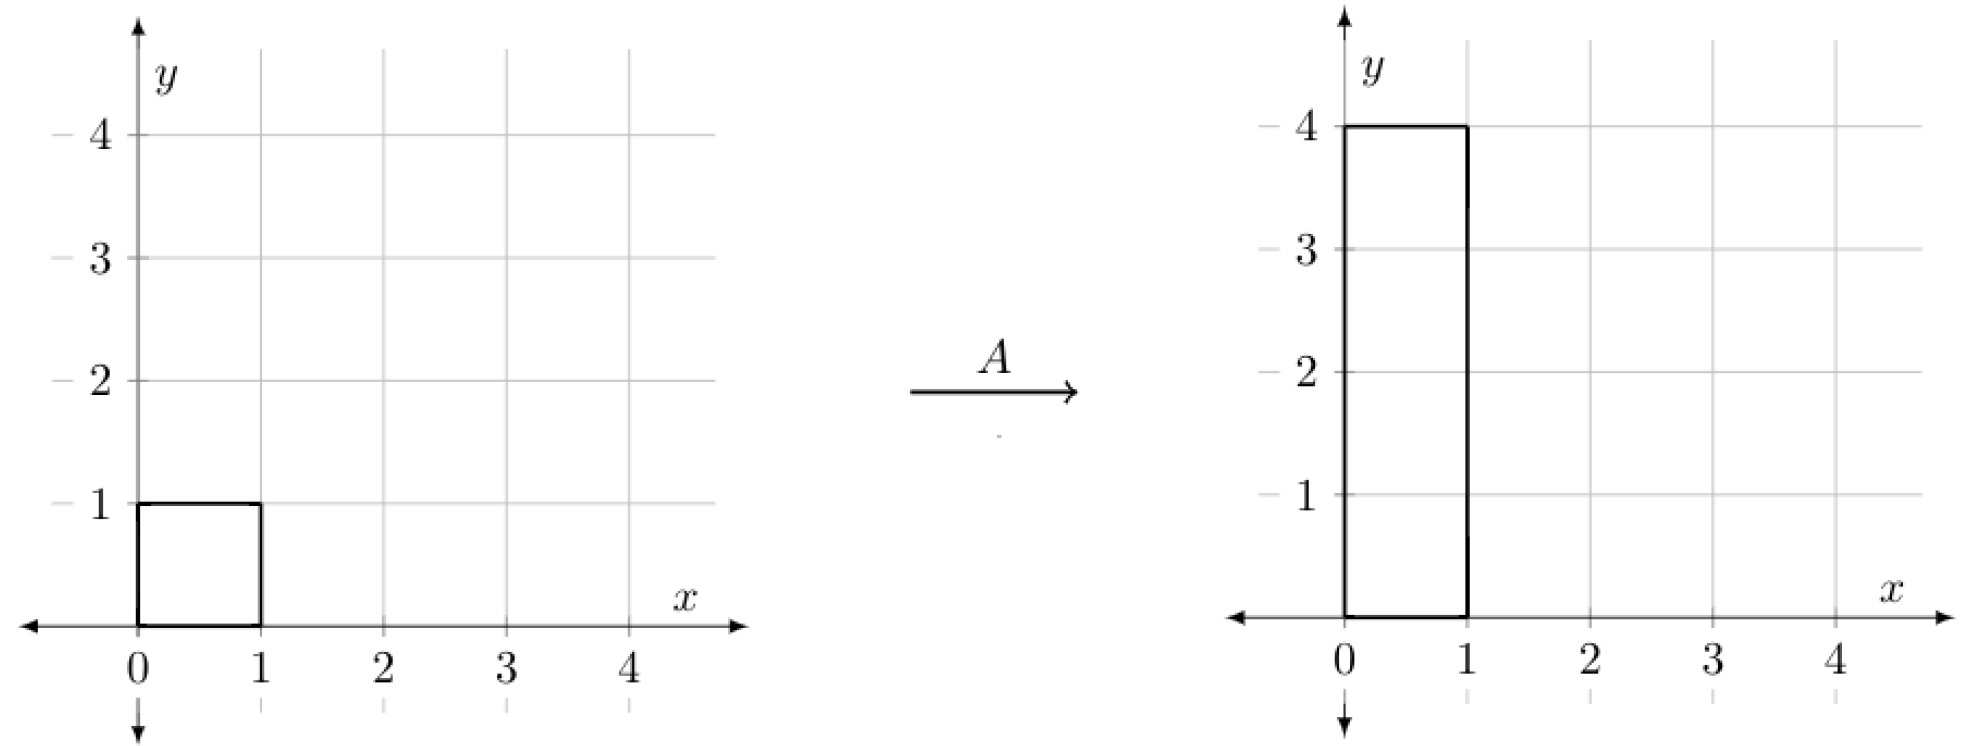
\includegraphics[scale=.6]{img/TransformationA.jpg}
\end{center}

So:  multiplication by a diagonal matrix is easy to understand.

What about $B = \mat{3&-1\\-2&2}$?  Applying this to
the same four points of the unit square $(0,0)$, $(0,1)$, $(1,0)$ and $(1,1)$
yields
$$
(0,0), (-1,2), (3,-2), (2,0)
$$
which is a completely different parallelogram, as in the figure below:

\begin{center}
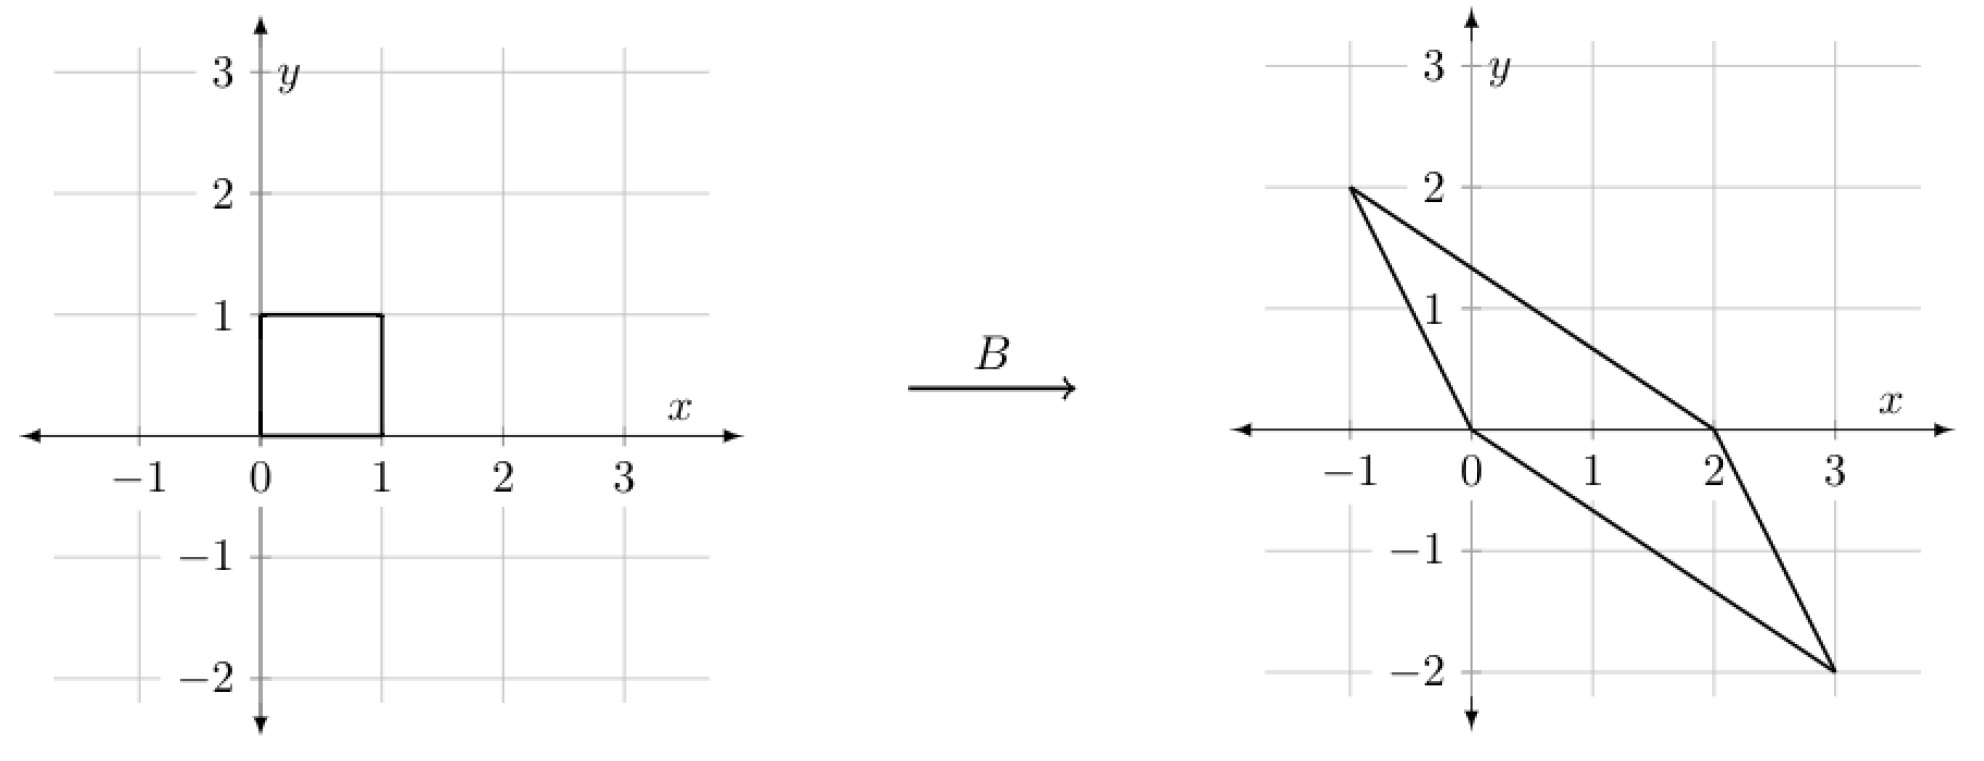
\includegraphics[scale=.6]{img/TransformationB1.jpg}
\end{center}

But what does it mean?  

The secret is in the eigenvectors.  They are $(1,2)$ (corresponding
to eigenvalue 1) and $(-1,1)$ (corresponding to eigenvalue 4).
So if we were to draw a parallelogram with vertices
$$
(0,0), (1,2), (-1,1), (0,3)
$$
then after multiplication by $B$, you'd get
$$
(0,0), (1,2), (-4,4), (-3, 6)
$$
which makes sense when you sketch it, as in the figure below:

\begin{center}
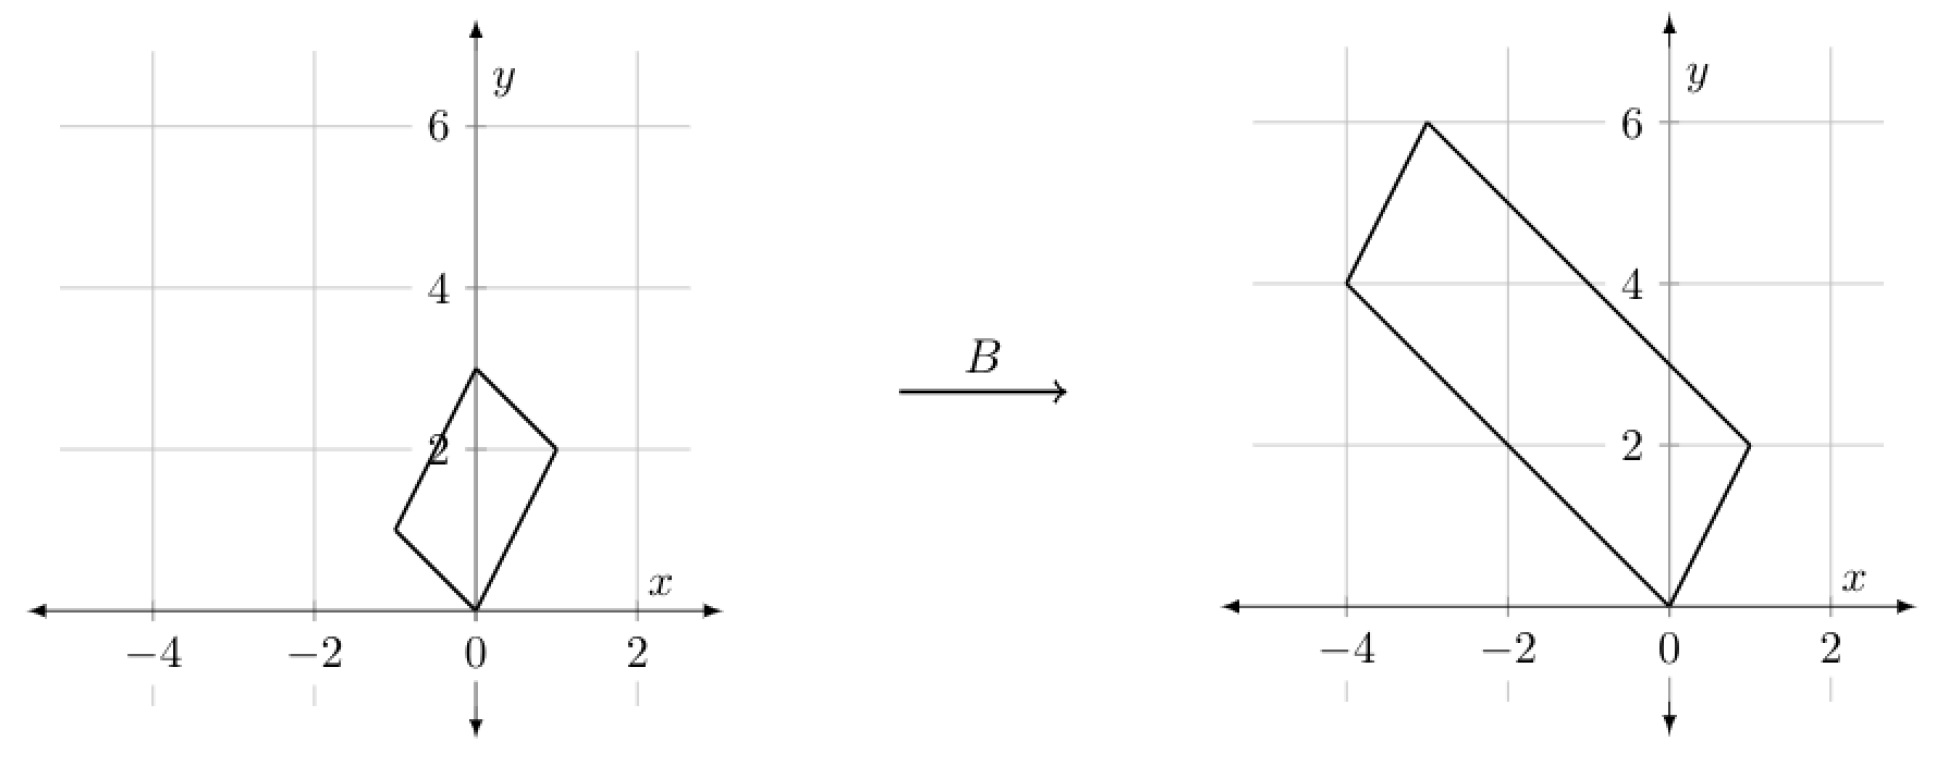
\includegraphics[scale=.6]{img/TransformationB2.jpg}
\end{center}

Multiplication by $B$ stretch the parallelogram
by a factor of $4$ in the direction $(-1,1)$ (and by a factor of $1$ in the direction $(1,2)$).
Looking back, this also explains what happened to our standard unit square:  it
was stretched along the axis $\spn\{(-1,1)\}$.

The point:  the basis of eigenvectors is the secret to understanding
the geometry of multiplication by $A$.
\end{myexample}

Viewing $A$ as a transformation in this way --- as a \stress{linear transformation} --- is fundamental to discrete time dynamical systems see  `Markov processes in probability'\footnote{Search the web for  `Markov chain'.}.


What we want to do next:  explore this idea of linear transformations in
greater detail, and get back to that picture we once used in class,
illustrating the nullspace and column space of a matrix via a map from
$\R^n$ to $\R^m$ (the map being:  multiplication by $A$).




\section*{Problems}
\addcontentsline{toc}{section}{Problems}

 


\medskip {\bf Remarks:} 
\begin{enumerate}
\item A question with an asterisk `$ ^\ast$' (or two) indicates a bonus-level question.
 \item You must justify all your responses.
\end{enumerate}
\bigskip


\begin{prob} \label{prob23.1} 
\begin{enumerate}[a)]
\item For each of the matrices $A$  in Problem \ref{prob22.1}, if possible, find an invertible matrix $P$ and a diagonal matrix $D$ such that $P^{-1}AP =D$. If this is not possible, explain why. (Solutions to parts b, d, f and h are available.) 

\item Use the fact that $A=\bmatrix 
1&0&1\\0&1&0\\1&1&1 \endbmatrix $ is diagonalizable to compute  $A^{10^{1000}}$ before the sun becomes a red giant and (possibly) engulfs the earth.\footnote{You have between 5 and 6 billion years, but it should only take you less than 5 minutes.} 

\end{enumerate}

 

\end{prob} \begin{prob} \label{prob23.2} State whether each of the following is (always) true,
or is (possibly) false.     
   \smallskip    
\begin{enumerate}[$\bullet$]
\item If you say the statement may be false, you must give an explicit example.   
\item If you say the statement is true, you must give a clear explanation -   by quoting a theorem presented in class, or by giving a {\it proof valid for every  case}. 
\end{enumerate}

\begin{enumerate}[a)]
\item If $3$ is an eigenvalue of an $n \times n$ matrix $A$, there must be a non-zero vector $\vv \in \R^n$ with $Av=3v$.
\medskip
%
\item\sov The matrix $\bmatrix 0&-1\\1&0\endbmatrix$ has no real eigenvalues.
\medskip
%

\item The matrix $\bmatrix -1&1\\0&-1\endbmatrix$ is
diagonalizable.
\medskip
%
\item\sov If $0$ is an eigenvalue of  $n \times n$ matrix  $A$, then $A$ is
not invertible.
\medskip
%
\item If an  $n \times n$ matrix  $A$ is
not invertible, then $0$ is an eigenvalue of $A$.
\medskip
%
\item\sov Every invertible matrix is diagonalizable.
\medskip
%
\item Every diagonalizable  matrix is invertible.
\medskip
%
\item\sov If an $n \times n$ matrix has $n$ distinct eigenvalues, then the matrix is diagonalizable. 
\medskip
%
\item If an $n \times n$ matrix is diagonalizable then it must have $n$ distinct eigenvalues. 
\medskip
%
\item\sov\footnote{ Hint: Use the fact that we know $\det(A-\lam I_n)=(-1)^n(\lam-\lam_1)(\lam-\lam_2)\dots(\lam-\lam_n) $.} If an  $n \times n$ matrix  $A$ has eigenvalues $\lam_1, \dots ,\lam_n$, then $\det A=\lam_1 \dots\lam_n $.
\medskip
%

\item$^{\ast}$ If $\vv$ and $\ww$ are eigenvectors of a symmetric matrix $A$ (i.e. $A=A^T$) which correspond to different eigenvalues, then $\vv \cdot \ww=0$.\footnote{ Hint:  Remember that because $A$ is symmetric, $A\vv\cdot \ww=\vv\cdot A\ww$ (by Problem~\ref{prob14.4}). Now simplify both sides using the fact that $\vv$ and $\ww$ are eigenvectors and see what you obtain.}
\medskip
% 
\end{enumerate}
\end{prob} \begin{prob} \label{prob23.3}\sov Let $A=\bmatrix
0&1&1\\ 1&0&1\\ 1&1&0 \endbmatrix$. 

\begin{enumerate}[a)]

\item Compute $\det(A-\lam I_3)$ and hence show that the eigenvalues of
$A$ are $2$ and $-1$.

\item Find a basis of $E_2 =\set{\xx\in \R^3 \st A\xx= 2\xx}$.
\item Find a basis of $E_{-1} =\set{\xx\in \R^3 \st A\xx=-\xx}$. 
 
\item Find an invertible  matrix 
$P$ such that $P^{-1}AP=D$ is diagonal,  and give this diagonal matrix $D$. Explain why
your choice of $P$ is invertible.
\item Find an invertible  matrix 
$Q \not=P$ such that $Q^{-1}AQ=\tilde D$ is also diagonal,  and give this diagonal matrix $\tilde D$.
\end{enumerate}
  


\end{prob} \begin{prob} \label{prob23.4} $^{\ast}$\footnote{ This example is a simplified version of the equations of motion for 2 masses connected by springs. Search the web for `Normal mode' for an example. } Consider the coupled  system of second order differential equations for the the two functions $f$ and $g$:

$$\begin{matrix} 
\ddot f=-2 f +g  \\
\ddot g=f-2g\\
 \end{matrix} $$(Here $\ddot f$ and $\ddot g$ denote $\dfrac{d^2 f}{dt^2}$ and $\dfrac{d^2 g}{dt^2}$ respectively.)
This can be also written in matrix form as: $\bmatrix \ddot f \,\\ \ddot g
 \endbmatrix =\bmatrix -2 & 1 \\
 1 & -2 \endbmatrix \bmatrix  f \,\\   g
 \endbmatrix$. 
Let $A=\bmatrix -2 & 1 \\
 1 & -2 \endbmatrix $. Diagonalize $A$ to  write $A=PDP^{-1}$ for some invertible matix $P$ and some diagonal matrix $D=\bmatrix \lam_1 & 0 \\
 0 & \lam_2 \endbmatrix $. Now define two new functions $h$ and $k$ by  $\bmatrix h \,\\ k
 \endbmatrix = P^{-1} \bmatrix  f \,\\   g
 \endbmatrix$. Show that $\bmatrix \ddot f \,\\ \ddot g
 \endbmatrix =\bmatrix -2 & 1 \\
 1 & -2 \endbmatrix \bmatrix  f \,\\   g
 \endbmatrix$ is equivalent to $\bmatrix \ddot h\,\\ \ddot k
 \endbmatrix =\bmatrix \lam_1 & 0 \\
 0 & \lam_2 \endbmatrix\bmatrix  h \,\\   k
 \endbmatrix$, or, written out fully as
$$\begin{matrix} 
\ddot h=\lam_1 \,h  \\
\ddot k=\lam_2 \,k\\
 \end{matrix} $$ 

  You will find that both $\lam_1$ and $\lam_2$ are negative, so the solutions to these two (linear) second order differential equations\footnote{ Search the web  for `Linear differential equation' for some details.} are $h(t)=a \sin( \sqrt{|\lam_1|}\,t) + b \cos( \sqrt{|\lam_1|}\,t)$ and $k(t)=c \sin( \sqrt{|\lam_2|}\,t) + c \cos( \sqrt{|\lam_2}|\,t)$, where $a,b,c,d$ are real constants.

\medskip
  Use this to find $f$ and $g$, and solve for $a,b,c$ and $d$  in terms of  the so-called {\it `initial conditions' $f(0), \dot f(0), g(0), \dot g(0)$}.
\medskip
%


\end{prob}




%----------------------------------------------------------------------------------------
%	PART VI: Linear Transformations
%----------------------------------------------------------------------------------------

\chapterimage{Pinery.jpg} % Chapter heading image
%Pinery20070816.jpg

\renewcommand{\partintrotext}{In mathematics, one might begin by studying the objects under consideration --- in this case, vector spaces --- but then equally important is to understand the maps between them, that is, the maps that are ``compatible'' with the vector space structure.  These maps are called \stress{linear transformations}.  We have seen and used several already: the coordinate map, the projection map.}

\part{Linear Transformations}
%%%%%%%%%%%%%%%%%%%%%%part.tex%%%%%%%%%%%%%%%%%%%%%%%%%%%%%%%%%%
% 
% sample part title
%
% Use this file as a template for your own input.
%
%%%%%%%%%%%%%%%%%%%%%%%% Springer %%%%%%%%%%%%%%%%%%%%%%%%%%

\begin{partbacktext}
\part{Linear Transformations}
\noindent In mathematics, one might begin by studying the objects under consideration --- in this case, vector spaces --- but then equally important is to understand the maps between them, that is, the maps that are ``compatible'' with the vector space structure.  These maps are called \stress{linear transformations}.  We have seen and used several already: the coordinate map, the projection map.

\end{partbacktext}

\chapter{Linear transformations}
\label{chapter:24LT}


Last time, we considered the geometric interpretation of ``multiplication
by $A$'':  it is a transformation of $\R^n$.   It's a special
kind of transformation:  it takes squares to parallelograms (as opposed
to anything else your imagination could provide!).

The key properties that made this work:
\begin{itemize}
\item $A\zero = \zero$
\item $A(\uu + \vv) = A\uu + A\vv$ for any $\uu,\vv \in \R^n$
\item $A(r\uu) = r(A\uu)$, for any $\uu\in\R^n$, $r\in\R$
\end{itemize}
These properties imply that the four points
of a parallelogram with vertices 
$$
\zero,\quad \uu,\quad \vv, \quad\uu+\vv
$$
 are
sent to the four points 
$$
\zero,\quad A\uu, \quad A\vv, \quad A\uu + A\vv
$$
(which again define the corners of a parallelogram, although it could
be degenerate (a line segment) if $A\uu$ and $A\vv$ are linearly
dependent); and moreover
that the straight line $r\uu$ is sent onto the straight line
$r(A\uu)$ (and similarly for the line through $\vv$).


\begin{definition}
Let $U$ and $V$ be vector spaces.  A \defn{linear transformation} $T$
is a map from $U$ to $V$ satisfying 
\begin{enumerate}
\item for all $\uu,\vv\in U$, $T(\uu+\vv) = T(\uu)+T(\vv)$
\item for all $\uu \in U$, $r\in\R$, $T(r\uu) = rT(\uu)$
\end{enumerate}
\end{definition}

We use the word \stress{transformation} here, and \stress{map};
we could use \stress{function} but that's often reserved for
a map whose range is the real numbers.  Whatever the terminology,
the point is that $T$ is a black box or formula or rule which
accepts a vector of $U$ as input, and produces a (uniquely determined) 
vector in $V$
as output; and furthermore we stipulate that it takes sums to sums
and scalar multiples to scalar multiples.  

So:  multiplication by a square matrix $A$ is a linear transformation.

We must now ask ourselves:  what other kinds of linear transformations
do we know?



\section{Examples of linear transformations}

\begin{myexample} \label{ex:multmatlintrans} Let $A$ be an $m\times n$ matrix.  Define the map
$$T \colon \R^n \to \R^m
$$
by $T_A(\uu) = A\uu$.  We claim that $T_A$ is a linear tranformation.

To prove this, we need to verify that:
\begin{enumerate}
\item for any $\uu,\vv \in \R^n$, $T_A(\uu+\vv) = T_A(\uu) +T_A(\vv)$:
$$
T_A(\uu+\vv) = A(\uu + \vv) = A\uu + A\vv =  T_A(\uu) +T_A(\vv)
$$
as required.
\item for any $\uu \in \R^n$, $r\in \R$, $T_A(r\uu) = rT_A(\uu)$:
$$
T_A(r\uu) = A(r\uu) = r(A\uu) = rT_A(\uu)
$$
as required.
\end{enumerate}
So this is a linear transformation, for any $m,n$ and $A$.
\end{myexample}

\begin{myexample} Consider the projection onto the plane $W$ given by
$$
W = \{ (x,y,z) \mid x-z = 0\}
$$
Let's first find a formula for this projection.  The easy way
is to note that $W^\perp = \spn\{(1,0,-1)\}$ so for $\uu = (u_1,u_2,u_3)\in \R^3$, we have
$$
\proj_{W^\perp}(\uu) = \frac{\uu \cdot (1,0,-1)}{(1,0,-1)\cdot (1,0,-1)} \mat{1\\0\\-1}
= \frac{u_1-u_3}{2}\mat{1\\0\\-1}
$$
and therefore
$$
\proj_W(\uu) = \uu - \proj_{W^\perp}(\uu) =\mat{u_1\\u_2\\u_3} - \frac{u_1-u_3}{2}\mat{1\\0\\-1} = \frac12\mat{u_1+u_3\\ 2u_2 \\ u_1+u_3}.
$$

Now is this a linear transformation?  We verify the two properties of
linearity (with $T = \proj_W$):
\begin{enumerate}
\item Is $\proj_W(\uu + \vv) = \proj_W(\uu) + \proj_W(\vv)$?  Let $\uu = (u_1, u_2, u_3)$ and $\vv = (v_1, v_2, v_3)$; then
\begin{align*}
\proj_W(\uu + \vv) &= \proj_U(u_1+v_1,u_2+v_2,u_3+v_3) \\
&= \frac12\mat{ (u_1+v_1) + (u_3+v_3)\\ 2(u_2+v_2)\\  (u_1+v_1) + (u_3+v_3)}\\
&= \frac12\left( \mat{u_1+u_3\\2u_2\\u_1+u_3} + \mat{v_1+v_3\\2v_2\\v_1+v_3}\right) \\
&= \frac12\mat{u_1+u_3\\2u_2\\u_1+u_3} + \frac12\mat{v_1+v_3\\2v_2\\v_1+v_3}\\
&= \proj_W(\uu) + \proj_W(\vv)
\end{align*}
as required
\item Is $\proj_W(r\uu) = r\proj_W(\uu)$?  Let $r\in \R$ and $\uu$ as above,
then
\begin{align*}
\proj_W(r\uu) &= \proj_W(ru_1,ru_3,ru_3)\\
&= \frac12\mat{ru_1+ru_3\\ 2ru_2 \\ ru_1+ru_3}\\
&= r\left(\frac12\mat{u_1+u_3\\ 2u_2 \\ u_1+u_3}\right)\\
&= r\proj_W(\uu)
\end{align*}
\end{enumerate}
Since both axioms are satisfied, this is a linear transformation.
\end{myexample}

\begin{myexample} Show that the map $T \colon \R^2 \to \R^2$ given by
$T(x,y) = (x+1, xy)$
is not a linear transformation.

It suffices to show that there exists even one pair of vectors $\uu,\vv$
for which $T(\uu+\vv) \neq T(\uu)+T(\vv)$; OR to show that there is
even one vector and one scalar for which $T(r\uu) \neq rT(\uu)$.
Let's show that in fact these axioms fail for almost all vectors
and scalars!

\begin{enumerate}
\item Note that $$T(\uu + \vv) = T(u_1+v_1,u_2+v_2) = (u_1+v_1+1, (u_1+v_1)(u_2+v_2))$$ whereas
$$
T(\uu) + T(\vv) = (u_1+1,u_1u_2) + (v_1+1, v_1v_2) = (u_1+v_1+2, u_1u_2+v_1v_2)
$$
but the first components can NEVER be equal (and the second components are only equal if the ``cross terms'' are zero).

So, for example, $T(1,0)=(2,0)$, $T(0,1)=(1,0)$ and $$T(1,1)=(2,1) \not=(2,0)+(1,0)=T(1,0) +T(0,1).$$

We could stop now: we've found an example that shows $T$ is not linear. But let's show that $T$ doesn't satisfy the second condition either.
\item Note that 
$$
T(r\uu) = T(ru_1,ru_2) = (ru_1+1, (ru_1)(ru_2)) = (ru_1+1, r^2u_1u_2)
$$
whereas
$$
rT(\uu) = r(u_1+1,u_1u_2) = (ru_1+r, ru_1u_2)
$$
but the first component is equal only when $r=1$ and the second only when
either $r=1$ or $r=0$ or $u_1u_2=0$. 

So, for example, $T(1,1)=(2,1)$, but $$T(2(1,1))=T(2,2)=(3, 4)\not= 2(2,1)=2\, T(1,1).$$
\end{enumerate}
So this map is defintely not linear.
\end{myexample}


\section{Constructing and describing linear transformations}

Checking the linearity of a map is eerily similar to the subspace test.  Is it the same thing?  NO: the
subspace test is for sets, but linear transformations are maps
between vector spaces (or subspaces).

The phrase ``linear transformation'' comes about in part because
the second property implies that the image under $T$ of a line
through the origin is again a line through the origin (or just $\set{0}$).

In particular, taking $r=0$, we deduce that for any linear
transformation, $T(\zero) = \zero$.

But the two properties imply much more:  they say that linear
combinations are sent to linear combinations, in the following
sense.

\begin{theorem}[Determination of Linear Transformations on a Basis]\label{Thm:LTbasis} \index{determination of a linear transformation on a basis}~
\begin{enumerate}
\item Suppose $T \colon U \to V$ is a linear transformation and
$\{ \uu_1, \cdots, \uu_n\}$ is a basis for~$U$.  Then $T$
is completely determined by the vectors $T(\uu_1)$, $\cdots$,
$T(\uu_n)$.
\item Suppose  $\{ \uu_1, \cdots, \uu_n\}$ is a basis for $U$
and $\{ \vv_1, \cdots, \vv_n\}$ are ANY $n$ vectors in $V$ (even
possibly dependent or $\zero)$.  Then there is a unique linear
transformation~$T$ which satisfies $T(\uu_i)=\vv_i$ for all $i$.
\end{enumerate}
\end{theorem}

\begin{proof}
\begin{enumerate}
\item What we mean by ``completely determined'' is:  we can
determine $T(\uu)$, without having a formula for $T$, IF we
know the vectors $T(\uu_1)$, $\cdots$,
$T(\uu_n)$.  Namely, let $\uu \in U$ be arbitrary.  Since
$\{ \uu_1, \cdots, \uu_n\}$ is a basis for $U$, we can
write
$$\uu = a_1\uu_1+\cdots+a_n\uu_n.$$
Then
$$
T(\uu) = T(a_1\uu_1+\cdots+a_n\uu_n) = a_1T(\uu_1) + \cdots + a_nT(\uu_n),
$$
as we wanted to show.
\item We need to give a rule for a map $T$ which sends $\uu_i$ to $\vv_i$.
We use the idea above:  for any $\uu \in U$, write $\uu = a_1\uu_1+\cdots+a_n\uu_n$.  Then define
$$
T(\uu) = a_1\vv_1 + \cdots + a_n\vv_n.
$$
This gives a function from $U$ to $V$ and you can check that it
is linear (try it!).
\end{enumerate}
\end{proof}

This theorem is very powerful.  Much in the same way that proving
the existence of a basis of any vector space simplified things
by showing that every $n$-dimensional vector space is really
just $\R^n$ in disguise, this theorem implies that every
linear transformation is just matrix multiplication in disguise!

\begin{theorem}[The standard matrix of a linear transformation]\index{standard matrix of a linear transformation}\label{thm:standt_mat}

Let $T \colon \R^n \to \R^m$ be a linear transformation.  Then
there is an $m\times n$ matrix $A$ such that
$$
T(\xx) = A\xx
$$
for all $\xx \in \R^n$.  More precisely, if $\{\ee_1, \cdots, \ee_n\}$
is the standard basis for $\R^n$, then the matrix $A$ is
given by:
$$
A = \left[ T(\ee_1) \;  T(\ee_2)\; \cdots \;   T(\ee_n)\right].
$$
The matrix $A$ is called the \defn{standard matrix} of $\,T$.
 \end{theorem}



\begin{myexample}
Consider the projection $T = \proj_W$ onto the plane $W = \{(x,y,z)\mid x-z=0\}$; we saw earlier that $T(u_1, u_2,u_3) = \frac12(u_1+u_3,2u_2,u_1+u_3)$.

Construct the matrix as in the theorem:  $T(1,0,0) = (\frac12,0,\frac12)$, $T(0,1,0) = (0,1,0)$, $T(0,0,1) = (\frac12,0,\frac12)$, so
$$
A = \mat{\frac12 & 0 & \frac12\\ 0 & 1 & 0\\ \frac12 & 0 & \frac12}
$$
and we see directly that
$$
A\uu =  \mat{\frac12 & 0 & \frac12\\ 0 & 1 & 0\\ \frac12 & 0 & \frac12}\mat{u_1\\u_2\\u_3} = \frac12\mat{u_1+u_3\\2u_2\\u_1+u_3} = T(\uu)
$$
as required.

 
\end{myexample}

\begin{proof}
To see why it works, recall that if you have a vector
$$\uu = \mat{u_1 \\ u_2 \\ \vdots \\ u_n}
$$
then in fact 
$$
\uu = u_1\ee_1 + \cdots + u_n\ee_n.
$$
Thus $T(\uu)$, by Theorem~\ref{Thm:LTbasis}, %the theorem \emph{Determination of Linear Transformations on a Basis}, 
is 
$$
T(\uu) = u_1 T(\ee_1) + \cdots + u_nT(\ee_n).
$$
But taking linear combinations is just matrix multiplication,
so we have
$$
T(\uu) = \left[ T(\ee_1) \;  T(\ee_2)\; \cdots \;   T(\ee_n)\right]
\mat{u_1 \\ u_2 \\ \vdots \\ u_n} = A\uu.
$$
\end{proof}


\section{Kernels and images}

This new interpretation of the projection map as a linear transformation
gives us more geometric ideas about what the operation of projection
really does.  For instance, the projection map annihilates (sends to
$\zero$) any vector of $U^\perp$.  But it completely covers $U$
in the sense that ever point of $U$ is the image of some element under
$T$.

To state this more clearly, we need some definitions.

\begin{definition}
Let $T \colon U \to V$ be a linear transformation.  Then
\begin{itemize}
\item the \defn{kernel} of $T$, denoted $\ker(T)$, is the
set of all elements of $U$ which are sent to $\zero$ by $T$,
that is,
$$
\ker(T) = \{ \uu \in U \mid T(\uu) = \zero\}
$$
\item the \defn{image} of $T$, denoted $\im(T)$, is the set of all
elements of $V$ which are equal to $T(\uu)$ for some $\uu \in U$,
that is,
$$
\im(T) = \{ \vv \in V \mid \vv = T(\uu) \; \textrm{for some $\uu\in U$.}\}
$$
\end{itemize}
\end{definition}

Now both $\ker(T)$ and $\im(T)$ are subsets of vector spaces, and
the natural first question is: are they subspaces?  Answer:  YES,
and they're even familiar ones!

\begin{theorem}[Kernels and Images of the Standard Matrix]\index{kernel vs nullspace}\index{image vs nullspace}
Let $T \colon \R^n \to \R^m$ be a linear transformation with
standard matrix $A$.  Then
$$
\ker(T) = \Null(A) \qquad \textrm{and} \qquad \im(T) = \col(A).
$$
\end{theorem}

The first equality is clear once you recall that $T(\uu) = A\uu$;
and for the second, one should go back and look up the original
definition of $\col(A) = \im(A)$.

\section{A return to the rank-nullity theorem}

Note that the rank-nullity theorem\footnote{Some like to call this theorem {\it the conservation of dimension}: since the dimension of the subspace sent to $0$ ($\dim \ker T$) plus the dimension of the image of $T$ (``what's left''),  is the same the dimension you began with: $n=\dim U$. ``Total dimension is preserved."} can be restated, for
a linear transformation $T \colon U \to V$, as 
$$
\dim(\ker(T)) + \dim(\im(T)) = n
$$
where $n = \dim(U)$.  We interpret this as giving an
accounting of what $T$ does to the vectors in $U$.
If $T$ sends $U$ onto a subspace of $V$ of dimension
equal to $U$, then the kernel must be $\{\zero\}$.  On the
other hand, if the dimension of the image is smaller than $\dim U$, then
those `missing' dimensions had to go somewhere;
in fact, they ended up in the kernel of $T$, as the equation above suggests. 

For example. the projection onto the plane $W$ we saw
earlier has kernel equal to the 1-dimensional $W^\perp$
and image is all of (2-dimensional) $W$:  and $2+1=3 = \dim(\R^3)$.


Conversely, knowing that we can think about $T$ as a matrix
multiplication means that we know that a basis for $\im(T)$
is any basis for $\col(A)$ (and this is something that we
find easy to answer).

\section{A remark about the projection matrix}
When we calculated the projection onto a subspace before, one of our methods was:
\begin{itemize}
\item Create a matrix $B$ such that $\col(B) = W$
\item Solve $(B^TB)\xx = B^T\bb$.
\item $\proj_W(\bb) = B\xx$
\end{itemize}
Putting this all together:  Suppose $B$ has linearly independent
columns, so that $B^TB$ is invertible.  (This was a homework
exercise.)
Then
$$
\proj_W(\bb) = B(B^TB)^{-1}B^T\bb
$$
so the projection is given by multiplication by the matrix
$$
 B(B^TB)^{-1}B^T.
$$
Therefore, this must be the standard matrix of $T$!  You can
try this out for the example above.



\section*{Problems}
\addcontentsline{toc}{section}{Problems}


\medskip {\bf Remarks:} 
\begin{enumerate}
\item A question with an asterisk `$ ^\ast$' (or two) indicates a bonus-level question.
 \item You must justify all your responses.
\end{enumerate}
\bigskip

%\centerline{\bf \underbar{}}

 \begin{prob} \label{prob24.1} State whether each of the following defines a linear transformation.    
   \smallskip    
\begin{enumerate}[$\bullet$]
\item If you say it isn't linear, you must give an explicit example to illustrate.   
\item If you say it is linear, you must give a clear explanation -   by quoting a theorem presented in class, or by verifying the conditions in the definition {\it  in every  case}. 
\end{enumerate}
\medskip
\begin{enumerate}[a)]
\item  $T:\R^2 \to \R^3$ defined by $T(x,y)=(x, y, x+y)$
\medskip
%
\item\sov $T:\R^3 \to \R^2$ defined by $T(x,y,z)=(2 z+x, y)$
\medskip
%
\item $T:\R^2 \to \R^2$ defined by $T(x,y)=(x, x y)$
\medskip
%

\item\sov $T:\R^2 \to \R^2$ defined by $T(\vv)=\bmatrix 0&-1\\ 1&0 \endbmatrix \vv$
\medskip
%
\item $T:\R^3 \to \R^3$ defined by $T(\vv)= \vv\times (1,2,3)$, where `$\times$' denotes the cross product.
\medskip
%

\item\sov $T:\R^3 \to \R^3$ defined by $T(\vv)= \proj_{(1,1,-1)}(\vv)$.
\medskip
%
\item $T:\R^3 \to \R^3$ defined by $T(\vv)= v-\proj_{(1,1,-1)}(\vv)$.
\medskip
%
\item\sov $T:\R^3 \to \R^3$ defined by $T(\vv)= \proj_{\vv}(1,1,-1)$.
\medskip
%
\item $T:\R^3 \to \R^3$ defined by $T(\vv)= \big(\vv \cdot (1,1,-1)\big) (1,0,1)$.
\medskip
%
\item\sov $T:\R^3 \to \R^3$ defined by $T(\vv)= 2 \vv$.
\medskip
%
\item $T:\R^3 \to \R^3$ defined by $T(\vv)= \proj_H(\vv)$, where $H$ is the plane through the origin with normal $(1,1,0)$.
\medskip
%
\item\sov $T:\R^3 \to \R^2$ defined by $T(\vv)= A\vv$, where $A=\bmatrix 1&0&1\\ 1&2&3\endbmatrix$.
\medskip

\end{enumerate} 

\end{prob} \begin{prob} \label{prob24.2} In each of the following, find the standard matrix of $T$ and use it to give a basis for $\ker T$ and $\im T$ and verify the conservation of dimension.

\medskip
\begin{enumerate}[a)]
\item $T:\R^2 \to \R^3$ defined by $T(x,y)=(x, y, x+y)$
\medskip
%
\item\sov $T:\R^3 \to \R^2$ defined by $T(x,y,z)=(2 z+x, y)$
\medskip
%
\item $T:\R^3 \to \R^3$ defined by $T(\vv)= \vv\times (1,2,3)$, where `$\times$' denotes the cross product.
\medskip
%
\item\sov $T:\R^3 \to \R^3$ defined by $T(\vv)= \proj_{(1,1,-1)}(\vv)$.
\medskip
%
\item $T:\R^3 \to \R^3$ defined by $T(\vv)= \vv-\proj_{(1,1,-1)}(\vv)$.
\medskip
%
\item\sov $T:\R^3 \to \R^3$ defined by $T(\vv)= \proj_H(\vv)$, where $H$ is the plane through the origin with normal $(1,1,0)$.
\medskip
%
\end{enumerate}

\end{prob} \begin{prob} \label{prob24.3} State whether each of the following is (always) true,
or is (possibly) false.    
   \smallskip    
\begin{enumerate}[$\bullet$]
\item If you say the statement may be false, you must give an explicit example.   
\item If you say the statement is true, you must give a clear explanation -   by quoting a theorem presented in class, or by giving a {\it proof valid for every  case}. 
\end{enumerate}
\medskip
\begin{enumerate}[a)]
\item If $T:\R^3 \to \R^2$ is linear, then $\ker T \not= \set{0}$.
\medskip
%
\item\sov If $T:\R^4 \to \R^2$ is linear, then $\dim \ker T \ge 2$.
\medskip
% 
\item If $T:\R^4 \to \R^5$ is linear, then $\dim \im T \le 4$.
\medskip
%
\item\sov If $T:\R^3 \to \R^2$ is linear, and $\set{\vv_1,\vv_2} \subset \R^3$ is linearly independent, then $\set{T(\vv_1),T(\vv_2)} \subset \R^2$ is linearly independent.
\medskip
%
\item If $T:\R^3 \to \R^2$ is linear, $\ker T=\set{\zero}$, and $\set{\vv_1,\vv_2} \subset \R^3$ is linearly independent, then $\set{T(\vv_1),T(\vv_2)} \subset \R^2$ is linearly independent.
\medskip
%
\item\sov If $T:\R^3 \to \R^3$ is linear, and $\ker T=\set{\zero}$, then $\im T=\R^3$.
\medskip
%
\item If $T:\R^2 \to \R^3$ is linear, and $\ker T=\set{\zero}$, then $\im T=\R^3$.

\end{enumerate}

\end{prob} \begin{prob} \label{prob24.4}$^\ast$ State whether each of the following defines a linear transformation.    
   \smallskip    
\begin{enumerate}[$\bullet$]
\item If you say it isn't linear, you must give an explicit example to illustrate.   
\item If you say it is linear, you must give a clear explanation -   by quoting a theorem presented in class, or by verifying the conditions in the definition {\it  in every  case}. 
\end{enumerate}
 \medskip
\begin{enumerate}[a)]
\item $T: \PP \to \PP$ defined by $T(p)=p'$, where $p'$ denotes the derivative of $p$.
\medskip
%
\item\sov $T: \PP \to \PP$ defined by $T(p)(t)=\dsize \int_0^tp(s) ds$.
\medskip
%
\item $\tr: \M_{2\,2} \to \R$ defined by $\tr\bmatrix a&b\\c&d\endbmatrix = a+d.$
\medskip
%
\item\sov $\det: \M_{2\,2} \to \R$ defined by $\det \bmatrix a&b\\c&d\endbmatrix = ad-bc.$
\medskip
%
\item $T: \F(\R) \to \R$ defined by $T(f)=f(1)$.
\medskip
%
\end{enumerate}
\end{prob}

%----------------------------------------------------------------------------------------
%	PART VII: Solutions
%----------------------------------------------------------------------------------------

\chapterimage{Ottawa6.jpg}

\renewcommand{\partintrotext}{Try every question \stress{before} looking at the solution --- once you've seen a solution, you'll need a fresh new problem to learn from.}
\part{Solutions}


\Extrachap{Solutions to selected exercises}

%1 
\section*{Problems of Chapter~\ref{Chapter:01complex}}

\begin{sol}{prob01.1} Express the following complex numbers in  Cartesian form: $a + b \,i$, with $a, b \in \R$.
\medskip
\begin{enumerate}[a)]
\item    $(2+i)(2+2 i)=2+6i$ \medskip  
\item $ \dfrac 1{1+i}=\dfrac{1}{2}- \dfrac{1}{2} i$\medskip 
\item $  \dfrac{8+3i}{5-3i}=\dfrac{31}{34}-\dfrac{39}{34}i$\medskip 
\item $\dfrac{5+5 \,i}{1-i}= 5 i$\medskip
% 
\item $\dfrac{(1+2i)(2+5i)}{3+4i}=\dfrac{ 12}{25} +\dfrac{59}{25}i  $

\item $\dfrac{1-i}{2-i}+\dfrac{2+i}{1-i}= \dfrac{11}{10}+\dfrac{13 }{10}i$\smallskip
% 
\item $\dfrac 1{(1-i)(3-2i)}=\dfrac{1}{26}+\dfrac{5 }{26}i$
%
\end{enumerate}

\end{sol} 

\begin{sol}{prob01.2} Find the polar form of the following complex numbers: (i.e. either  as $r e^{i\theta}$ or as $r(\cos \theta + i \sin \theta)$, with $r\geq 0$ and $-\pi <\theta \leq \pi$)\medskip
\begin{enumerate}[a)]

\item ${3\sqrt{3}-3i}=6(\cos (-\pi /6)+i \sin (-\pi /6))=6\, e^{-\frac{\pi}{6}i} $
\item $\dfrac{3\sqrt{3}-3i} {\sqrt{2}+i\sqrt{2}}=3(\cos (-5\pi /12)+i \sin (-5\pi /12)) =3\, e^{-\frac{5\pi}{12}i} $

\item $\dfrac{1-\sqrt{3}\,i}{-1+i}=\sqrt{2}(\cos (11\pi/12)+i\sin (11\pi /12))=\sqrt{2}\, e^{\frac{11\pi}{12}i} $
\item $\dfrac{5+5\sqrt{3}\,i}{\sqrt{2}-\sqrt{2}\,i}=5(\cos (7\pi /12)+i\sin (7\pi/12))= 5\,e^{\frac{7\pi}{12}i}$
\item $\dfrac{3+3\sqrt{3}\,i} {-2+2i}=\dfrac{3\sqrt{2}}{2}(\cos (5\pi /12)-i\sin (5\pi/12))=\dfrac{3\sqrt{2}}{2}\,e^{\frac{5\pi}{12}i}$
\end{enumerate}

\end{sol} 


 

\begin{sol}{prob01.4}   If $z$ is a complex number,

(i)  Is it possible that $z={\bar z}$? \soln (Yes, iff $z\in \R$:if $z=a + b\, i$, then $z={\bar z}$ iff $a + b\, i = a - b\, i )$ iff $b=-b$ iff $z=a \in \R$.

(ii)  Is it possible that $|{\bar z}|>|z|$? \soln (No: $|{\bar z}|=|z|$, always: if $z=a + b\, i$, then $|z|=\sqrt{a^2+b^2}=\sqrt{a^2+(-b)^2} =|{\bar z}|$.)

(iii)  Is it possible that ${\bar z}=2z$? \soln(Yes, but only if $z=0$: If ${\bar z}=2z$, then by the previous part, $|z|=2 |z|$, so $|z|=0$. So $z=0$ too.)

\medskip Give  examples to illustrate your affirmative answers, and explanations if you say the statement is always false.
\end{sol}

%2
\section*{Problems of Chapter~\ref{Chapter:02vectors}}
 

\begin{sol}{prob02.3} If $A=(1,\ 2,\ 3),\ B=(-5,\ -2,\ 5),\ C=(-2,\ 8,\ -10)$
and $D$ is the midpoint of $\overline{AB}$, find the coordinates of the
midpoint of $\overline{CD}$.

\soln The position vector $v$ of the midpoint of $\overline{CD}$ is $v=(C+D)/2$. But as $D=(A+B)/2$, 
$v=(C+(A+B)/2)/2=(-2,\ 4,\ -3)$

\end{sol} \begin{sol}{prob02.4} Solve the following problems using the dot product.\medskip





(b) Find the angle between the vectors $ (0,\ 3,\ -3)$
and $ (-2,\ 2,\ -1)$.  \medskip

\soln If $\theta$ is the angle between these two vectors, then $$\cos \theta=\dfrac{(0,\ 3,\ -3)\cdot(-2,\ 2,\ -1)}{\| (0,\ 3,\ -3)\| \| (-2,\ 2,\ -1)\|}=\dfrac{9}{\sqrt{18}\sqrt{9}}=\dfrac{\sqrt{2}}{2}.$$ Hence $\theta= \dfrac{\pi}{4}$.
%  $\pi/4$ 


\end{sol} \begin{sol}{prob02.5}  Solve the following problems. \medskip


(a) If $u=(2,\ 1,\ 3)$ and $v=(3,\ 3,\ 3)$ find
 $\proj_{v}{u}$. 

\soln  $$\proj_{v}{u}=\dfrac{u\cdot v}{\|v\|^2}v=\dfrac{(2,\ 1,\ 3)\cdot (3,\ 3,\ 3)}{\|(3,\ 3,\ 3)\|^2}(3,\ 3,\ 3)=\dfrac{18}{27}(3,\ 3,\ 3)=(2,2,2).$$ \medskip
%${{2}\over{3}}(3,\ 3,\ 3)$
\\


(b)  If $u=(3,\ 3,\ 6)$ and $v=(2,\ -1,\ 1)$ find
the length of the projection of $u$ along $v$. 

\soln
$$\|\proj_{v}{u}\|=\dfrac{|u\cdot v|}{\|v\|^2}\|v\|=\dfrac{|u\cdot v|}{\|v\|}=\dfrac{(3,\ 3,\ 6)\cdot (2,\ -1,\ 1)}{\|((2,\ -1,\ 1))\|}=\dfrac{ 3}{ 2}\sqrt{6}.$$
 
(c) Find angle between the planes with Cartesian equations $x-z=7$ and $y-z=234$
\medskip

\soln The angle between two planes is always the acute angle between their normal lines. So we find the angle $\varphi$ between their normals ($1,0,1$ and $(0,1,-1)$ and adjust if necessary. The angle $\varphi$ is $\dfrac{2\pi}{3}$, so the answer is $\pi -\dfrac{2\pi}{3}=\dfrac{\pi}{3}$
%$\pi/3$.

\medskip
%$(3\sqrt6)/2$
 
  
\end{sol}  
 
%3
\section*{Problems of Chapter~\ref{Chapter:03linesplanes}}
\begin{sol}{prob03.1}  Solve the following problems using the cross and/or dot products.\medskip
  
 
(b) Find all vectors in $\R^3$ which are orthogonal to both  $(-1, 1, 5)$ and $(2, 1, 2)$.  \medskip

\soln Such vectors will be parallel to the cross product of these two vectors, which is found to be $(-3, 12, -3)$. Hence $\{(t,\ -4t,\ t)|\ t\in \R\}$ is the solution.
 
\medskip

 

(d) If $u=(-4,\ 2,\ 7),\ v=(2,\ 1,\ 2)$ and 
$w=(1,\ 2,\ 3)$, find $u\cdot (v\times w)$. \medskip

\soln This is $(-4,\ 2,\ 7)\cdot (2,\ 1,\ 2)\times (1,\ 2,\ 3)= (-4,\ 2,\ 7)\cdot (-1, -4, 3)=17$.
% 17
 \end{sol}
 
\begin{sol}{prob03.2}  Solve the following problems using the appropriate products.\medskip


(b) Find the area of the triangle with vertices $A=(-1,\ 5,\
0)$, $B=(1,\ 0,\ 4)$ and $C=(1,\ 4,\ 0)$ 

\soln This will be $\dfrac12$ the length of the cross product of the two vectors $B-A$ and $C-A$, and so is  $\dfrac12\|(4, 8, 8)\|=6$.  
%6

\medskip
(d) Find the volume of the parallelepiped  determined by $u=(1,\ 1,\ 0),\ v=(1,\ 0,\ -1)$ and $w=(1,\ 1,\ 1)$.

\soln This is simply the absolute value of $u \cdot v \times w$ and so is $1$.
% 1


\end{sol} \begin{sol}{prob03.3}  Solve the following problems. \medskip

(a) Find the point of intersection of the plane with Cartesian equation $2x+2y-z=5$,
and the line with parametric equations $x=4-t,\ y=13-6t,\ z=-7+4t$.  

\soln Once we substitute $x=4-t,\ y=13-6t$ and $ z=-7+4t$ into $2x+2y-z=5$, we can solve for $t$, which we then substitute backinto $x=4-t,\ y=13-6t$ and $ z=-7+4t$ to obtain $(2,\ 1,\ 1)$.\medskip
%$(2,\ 1,\ 1)$

\medskip

(b) If $L$ is the line passing through $(1,\ 1,\ 0)$ and $(2,\
3,\ 1)$, find  the point of intersection of $L$ with the plane with Cartesian equation $x+y-z=1$. 

\soln We find the (scalar) parametric equations for the $L$, and then proceed as in part (a) to obtain $(1/2,0,\ -1/2)$


\medskip

(d) Do the planes with Cartesian equations $2x-3y+4z=6$ and $4x-
6y+8z=11$ intersect? 

\soln No, their normals are parallel, so the planes are, but their equations are not multiples of the other.\medskip

\medskip


(f) Find the line of intersection of the planes with Cartesian equations $x+11y-4z=40$ and $x -y=-8$. 

\soln A direction vector for this line will be perpendicular to both normal vectors, and so can be obtained as the cross product of these normals, namely $(-4, -4, -12)$. (We will choose $(1,1,3)$ instead.) Now all we need to do is find one point on this line. This is done by substituting $x= y-8$ into $x+11y-4z=40$, and simplifying to obtain $3y-z=12$. Now set $z=0$, to obtain the point $(-4,\ 4,\ 0)$. Hence the line is $\set{(-4,\ 4,\ 0)+ t (1,\ 1,\ 3),\st  t\in \R}$\medskip
%$(-4,\ 4,\ 0)+ t (1,\ 1,\ 3),\, t\in \R$

 

\end{sol} 
\begin{sol}{prob03.4}  Solve the following problems. \medskip



(b)  Find the distance from the point $Q=(-2,\ 5,\ 9)$ to the plane with Cartesian equation
$6x+2y-3z=-8$ 

\soln Choose any point $P$ on the plane - say $P=(0,-4,0)$. The the distance between $Q$ and the plane is the length of the projection of $QP$ in the direction of the normal $(6,2,-3)$. This length is $\Big|\dfrac{(Q-P)\cdot(6,2,-3)}{\|(6,2,-3)\|}\Big|=3.$ \medskip

\medskip


(d)  Find the distance from the point $P=(8,\ 6,\ 11)$ to the
line containing the points $Q=(0,\ 1,\ 3)$ and $R=(3,\ 5,\ 4)$. 

\soln Draw a picture: this will be the smaller of the lengths of the vectors $(Q-P)\pm \proj_{R-Q}(Q-P)$. Alternatively, we could solve for $s$ in $0=(R-Q)\cdot(P-(Q+ s (R-Q))$ to find the point $S=Q+ s (R-Q)$ on the line closest to $P$, and then compute $\|P-S \|$. In either case, the answer is $7$. \medskip
% 7





\end{sol} 


\begin{sol}{prob03.5}  Find the scalar {\it and} vector parametric forms for  the following lines:
\medskip


(b)  The line containing $(-5,\ 0,\ 1)$ and which is parallel to the two planes with Cartesian equations $2x-4y+z=0$ and  $x-3y-2z=1$. 

\soln This line will be perpendicular to both normals, and so parallel to the cross product of the normals. Hence the scalar parametric form is $x=-5+11t,\, y=5t,\, z=1-2t,\, t\in \R$, and the vector parametric form is $(-5,\ 0,\ 1) + t(11,5,-2)$.\medskip

\end{sol} 
\begin{sol}{prob03.6}  Find a Cartesian equation for each of the following planes:

\medskip

(b)   The plane parallel to the vector $(1, 1, -2)$  and containing  the points $P=(1, 5, 18)$ and $Q=(4, 2, -6)$  
$5x - 3y + z = 8$. 

\soln This will be the plane through $P$ with normal parallel to the cross product of $(1, 1, -2)$ and $P-Q$. An easy computation then yields the equation $5x - 3y + z = 8$ (after dividing by 6).
\medskip

 

(d)  The plane containing the   two lines 
$ \set{(t-1,6-t,-4+3t)\st t \in \R}$ and  $ \set{(-3 -4t, 6+ 2t,  7+5t)\st \in \R} $     

\soln Pick a point on either line, say $P=(-1,6,-4)$. Then this will be the plane through $P$ with normal parallel to the cross product of the direction vectors of each line. An easy computation then yields the equation $11x + 17y + 2z = 83$.
\medskip 

 

(f) The plane containing the point $P=(1, -1, 2)$  and the line $\set{(4, -1 + 2t,2 + t)\st t \in \R}$.\soln Pick a  point on the line, say $Q=(4,-1,2)$. This will be the plane through $P$ with normal parallel to the cross product of $P-Q$ and a direction vector for the line (say) $(0,2,1)$. One obtains (after division by $\pm3$) the equation $y - 2z =- 5$.\medskip
% 

 

(h) The plane containing the point $P=(1,\ -7,\ 8)$ which is perpendicular to the line $\set{(2+2t,7-4t,-3+t\st  t\in \R}.$ \soln This will be the plane through $P$ with normal paralle to a direction vector for the line. One obtains the equation $2x-4y+z=38$.\medskip  
%$2x-4y+z=38$ 

\end{sol}

 \begin{sol}{prob03.7} Find a vector parametric form  for  the planes with Cartesian equations given as follows. (i.e. find some $a \in H$ and two non-zero, non-parallel vectors $u, v \in \R^3$, parallel to the plane $H$. Then  $H=\set{a+ s u + t v\st s,t \in \R}$.)\medskip

(b)  $x - y - 2z = 4$. 

\soln Take $a=(4,0,0) \in H$. To pick $u$ and $v$, simply choose two (non-zero, non-parallel) vectors perpendicular to a normal vector $(1,-1,-2)$. So  $u= (1,1,0)$  and $v=(2,0,1)$ will do. Then $H=\set{(4,0,0)+ s (1,1,0) + t (2,0,1)\st s,t \in \R}$. (There are of course infinitely many correct answers.)\medskip


\end{sol} 

\begin{sol}{prob03.8}  Let $u, v$ and $w$ be any vectors in $\R^3$.  Which  of the following statements could be false, and give an example to illustrate each of your answers.
 \medskip

(1)  $u\cdot v=v\cdot u$. \soln This is always true.

\medskip

(2)  $u\times v=v\times u$. \soln Since $u\times v=- v\times u$ always holds, this is only true if $u$ and $v$ are parallel or either is zero. So for a counterexample, take $u=(1,0,0)$ and $v=(0,1,0)$. Then $u\times v=(0,0,1)\not=(0,0,-1)=v \times u$

\medskip

(3)  $u\cdot(v+w)=v\cdot u+w\cdot u$. \soln This is always true. 

\medskip

(4)  $(u+2v)\times v=u\times v$. \soln This is always true, since $v\times v=0$ always holds.

\medskip

(5)  $(u\times v)\times w=u\times(v\times w)$. \soln This is almost always false. Indeed by the last question in this set of exercises, it is true only if $(u \cdot w)v- (u\cdot v) w = (w\cdot u) v- (w\cdot v) u \iff (u\cdot v) w = (w\cdot v) u$. So for a counterexample, take $u=(1,0,0)=v$ and $w=(0,1,0)$. Then $(u\times v)\times w=(0,0,0) \not=(0,-1,0)=u\times(v\times w)$.

% 2 \& 5

\end{sol}


 \begin{sol}{prob03.9}  Let $u , v $ and $w $ be vectors in $\R^3$.  Which of the following 
statements are (always) true? Explain your answers, including  giving examples to illustrate statements which could be false. 
\medskip

(i)  $(u\times v)\cdot v=0$. \soln This is always true: it is a property of the cross product which is easliy checked.
 
\medskip

(ii)  $(v\times u)\cdot v=-1$ \soln This is always false, and the left hand side is always zero. So take $u=v=0$.
 
\medskip

(iii)  $(u\times v)\cdot w$ is the volume of the of the parallelepiped  determined by $u$, $v$ and $w$. \soln Volumes are always positive, so this is only true if $(u\times v)\cdot w= |(u\times v)\cdot w|$; so if $u=(1,0,0), v=(0,1,0)$ and $w=(0,0,-1)$, $(u\times v)\cdot w=-1$, which is not the volume of the unit cube.  
 
\medskip

(iv)  $||u\times v||=||u||\,||v||\,\cos\theta$
where $\theta$ is the angle between $u$ and $v$. \soln This is only true if $\cos\theta=\sin \theta$, since it is always true that $||u\times v||=||u||\,||v||\,\sin\theta$, where $\theta$ is the angle between $u$ and $v$. So take $u=(1,0,0)$ and $v=(0,1,0)$ for a counterexample.

\medskip 

(v)  $|u\cdot v|=||u||\,||v||\,\cos\theta$
where $\theta$ is the angle between $u$ and $v$. \soln This is always true.
 
\end{sol} 




%4
\section*{Problems of Chapter~\ref{chapter:04vectorspaces}}

\begin{sol}{prob04.1} Determine whether   the following sets are closed under the indicated rule for addition. 

  

\medskip


(b)  $L=\set{(x, y) \in \R^2\st x -3y=0 }$; standard addition of vectors in $\R^2$. 

\soln This is closed under addition: Suppose $(x,y), (x',y')\in L$. Then $x -3y=0$ and $x' -3y'=0$. Since $(x,y)+ x',y')=(x+x', y+y')$ satisfies $x+x' -3(y+y')= (x -3y) +(x' -3y')=0+0=0$, we see that  $(x,y)+ (x',y')\in L$.\medskip
%
 

(d) $S=\set{(x, y) \in \R^2\st xy \ge 0 }$ ; standard addition of vectors in $\R^2$. 

\soln This is not closed under addition. For example, $(1,2)$ and $(-2,-1)$ both belong to $S$, but their sum, $(-1,1)$ does not.\medskip


(f)  $K=\set{(x, y, z) \in \R^3\st x+2y+z=1 }$ ; standard addition of vectors in $\R^3$. \soln This is not closed under addition. For example, both $(1,0,0)$ and $(0,0,1)$ belong to $K$ but their sum, $(1,0,1)$ does not.  \medskip 
%

 


(h)  $M=\set{(x, x+2) \in \R^2\st x\in \R}$; {\it Non-standard addition}: $(x,y) \tilde+ (x',y')=(x+x', y+y-2)$.  

\soln  This {\it is }closed under the weird addition rule (but not under the standard one- see part (a)): Let $u=(x, x+2)$ and $v=(x', x'+2)$ be any two points in $M$. Then $u \tilde+ v=(x+x', (x+2)+(x'+2)-2)=(x+x', x+x'+2) \in M$.\medskip

\end{sol} 

\begin{sol}{prob04.2} Determine whether each of the following sets is closed under the indicated rule for multiplication of vectors  by scalars.
 
\medskip
 

(b)  $L=\set{(x, y) \in \R^2\st x -3y=0 }$;  standard rule for multiplication of vectors  in $\R^2$ by scalars.  

\soln This is closed under multiplication by scalars: Let $u=(x,y)\in L$ (so $x -3y=0$) and $k\in \R$ be any scalar. Then $k u= (kx, ky)$ satisfies $kx-3(ky)=k(x-3y)=k0=0$, and so $ku\in L$.\medskip
%
 

(d)  $S=\set{(x, y) \in \R^2\st xy \ge 0 }$; standard rule for multiplication of vectors  in $\R^2$ by scalars. 

\soln This is closed under multiplication by scalars (despite not being closed under addition- see (d) in Q.1): Let $u=(x,y)\in S$ (so $xy \ge 0$) and $k\in \R$ be any scalar. Then $k u= (kx, ky)$ satisfies $kx(ky)=k^2 xy \ge 0$, since  $xy \ge 0$ and $k^2\ge 0$. So $ku\in S$. \medskip
%



(f) $K=\set{(x, y, z) \in \R^3\st x+2y+z=1 }$; standard rule for multiplication of vectors  in $\R^3$ by scalars. 

\soln This is not closed under multiplication by scalars. For example, $u=(1,0,0)\in K$ but $2u =(2,0,0)\notin K$\medskip 
%

 

(h)  $M=\set{(x, x+2) \in \R^2\st x\in \R}$; {\it Non-standard  multiplication of vectors  by  scalars $k\in \R$}: $$k\circledast (x,y)=(kx, ky-2k+2).$$   


\soln This {\it is} closed under this weird rule for multiplication of vectors  by  scalars (but not under the standard rule: see part (a)): Let $u=(x, x+2)\in M$, and $k\in \R$. Then$k\circledast u =k\circledast (x,x+2)= (kx, k(x+2)-2k+2)=(kx, kx+2) \in M$!
\medskip
  


\end{sol} 

\begin{sol}{prob04.3}  Determine whether   the following subsets of $\F(\R)=\set{f \st f: \R \to \R}$ are closed under the standard addition of functions in  $\F(\R)$. (Recall that $\F(\R)$ consists of all real-valued functions of a real variable; i.e., all functions with domain $\R$, taking values in $\R$). 
 \medskip
 
(b) $T=\set{f \in \F(\R) \st f(2)=1 }$. 

\soln This is not closed under addition: for example, the constant function $f(x)=1, \forall x\in \R$ belongs to $T$ but $f+f$, which is the constant function $2$, does not.
\medskip  



(d)  $N=\set{f \in \F(\R) \st \text{ for all } x\in \R,   \, f(x)\le 0}$. 

\soln This is closed under addition: Let $f, g \in N$ (so $\forall x \in \R, f(x)\le 0$ and $g(x)\le 0$. Then,  since the sum of two non-positve numbers is is still non-positive,  $\forall x \in \R,, (f+g)(x)= f(x)+g(x)\le 0$. Hence $f+g\in N$.\medskip 
%



(f) $O=\set{f \in \F(\R) \st \text{ For all } x\in \R,   \, f(-x)= -f(x)}$. 

\soln This is the set of all so-called `odd' functions, and it is closed under addition: Let $f,g \in O$. Then, $\forall x \in \R, f(-x)= -f(x)$ and $g(-x)= -g(x)$, so, $\forall x \in \R, (f+g)(-x)=f(-x)+g(-x)=-f(x)-g(x)=-(f(x)+g(x))=-(f+g)(x)$. Hence $f+g\in O$.\medskip 
%


\end{sol} 

\begin{sol}{prob04.4} Determine whether  the following sets are closed under the standard rule  for multiplication of functions  by scalars in $\F(\R)$. 
\medskip


(b)  $T=\set{f \in \F(\R) \st f(2)=1 }$. 

\soln This is {\it not} closed under multiplication by all scalars. For example, the constant function $1$ belongs to $T$, but if we multiply this function by the scalar 2, we obtain the constant function $2$, which does not belong to $T$. \medskip
% 



(d)  $\set{f \in \F(\R) \st \text{ For all } x\in \R,   \, f(x)\le 0}$. 

\soln This is {\it not} closed under multiplication by all scalars (despite being closed under addition - see part (d) in the previous question): for example, the constant function $g(x)=-1, \forall x\in \R$ belongs to $N$ but $(-1)g$, which is the constant function $1$, does not.\medskip 
%



(f)  $O=\set{f \in \F(\R) \st \text{ For all } x\in \R,   \, f(-x)= -f(x)}$. 

\soln This is  closed under addition: Let $f \in O$. Then, $\forall x \in \R, f(-x)= -f(x)$. Now let $k\in \R$ be any scalar. Then, $\forall x \in \R, (kf)(-x)=k (f(-x))=k(-f(x))=-kf(x)=-(kf)(x)$. Hence $kf\in O$. \medskip 
 


\end{sol} 

\begin{sol}{prob04.5} Determine whether   the following sets are closed under the standard operation of addition of matrices in $\M_{2 \,2}(\R)$. 
 \medskip





(b)  $S=\Bigg\{  \bmatrix a&b \\c&d\endbmatrix \in \M_{2 \,2}(\R) \;\Bigg|\; a+d=0\Bigg\}$. 

\soln This is closed under addition: suppose $A=\bmatrix a&b\\ c&d\endbmatrix$ and $b=\bmatrix a'&b'\\ c'&d'\endbmatrix$ belong to $S$. So $a+d=0$ and $a'+d'=0$. Then $A+B=\bmatrix a+a'&b+b'\\ c+c'&d+d'\endbmatrix$ satisfies $(a+a')+(d+d')= (a+d) +(a'+d')=0+0=0$, and so $A+B \in S$. \medskip
%




(d)  $U=\Bigg\{  \bmatrix a&b\\ c&d\endbmatrix \in \M_{2 \,2}(\R) \;\Bigg|\; ad=0\Bigg\}$.  

\soln This is not closed under addition: for example, $A=\bmatrix 1&0 \\0&0\endbmatrix$ and  $A=\bmatrix 0&0\\ 0&1\endbmatrix$ both belong to $U$, but $A+B= \bmatrix 1&0\\ 0&1\endbmatrix$ does not.\medskip
%



\end{sol} 

\begin{sol}{prob04.6} Determine whether   the following sets are closed under the  standard rule  for multiplication of matrices by scalars in $\M_{2 \,2}(\R)$. 
 \medskip




(b)  $\Bigg\{  \bmatrix a&b \\ c&d\endbmatrix \in \M_{2 \,2}(\R) \;\Bigg|\; a+d=0\Bigg\}$.  

\soln This is closed under multiplication  by scalars: suppose $A=\bmatrix a&b\\ c&d\endbmatrix$ belongs to $S$. So $a+d=0$. If $k\in\R$ is any scalar, Then $kA =\bmatrix ka &kb \\ kc & kd \endbmatrix$ satisfies $ ka + kd = k(a+d)=k0=0$, and so $kA \in S$.  \medskip
%

 

(d)  $U=\Bigg\{  \bmatrix a&b \\c&d\endbmatrix \in \M_{2 \,2}(\R) \;\Bigg|\; ad=0\Bigg\}$. 
  
\soln This {\it is} closed under multiplication  by scalars (despite not being  closed under addition - see part (d) of the previous question):  suppose $A=\bmatrix a&b\\ c&d\endbmatrix$ belongs to $U$. So $a  d=0$. If $k\in\R$ is any scalar, Then $kA =\bmatrix ka &kb \\ kc & kd \endbmatrix$ satisfies $ (ka)  (kd) = k^2(a d)=k^20=0$, and so $kA \in U$.    \medskip



\end{sol} 

\begin{sol}{prob04.7} The following sets have been given   the indicated rules for addition of vectors,  and multiplication of objects  by real scalars (the so-called  {\it `vector operations' }). If possible, check if there is a zero vector in the subset in each case. If it is possible, show your choice works in {\it all } cases, and if it is not possible, give an example to illustrate your answer. 

(Note: in the last two parts, since the vector operations are not the standard ones, the zero vector will probably not be the one you're accustomed to.)
 
\medskip
 

(b)  $L=\set{(x, y) \in \R^2\st x -3y=0 }$; standard  vectors operations in $\R^2$. 

\soln Since the operations are standard, the zero vector is the standard one, namely $(0,0)$. Since $0- 3(0)=0$, $(0,0)\in L$. \medskip
%




(d)  $S=\set{(x, y) \in \R^2\st xy \ge 0 }$;  standard  vectors operations in $\R^2$.  

\soln Since the operations are standard, the zero vector is the standard one, namely $(0,0)$. Since $0\, 0=0\ge 0$, $(0,0)\in S$. \medskip
%
 



(f)  $K=\set{(x, y, z) \in \R^3\st x+2y+z=1 }$; standard  vectors operations in $\R^3$. 

\soln Since the operations are standard, the zero vector is the standard one, namely $(0,0,0)$. However, $0+2(0)+0=0\not=1$, so $(0,0,0)\notin K$.\medskip 
%


(h) $M=\set{(x, x+2) \in \R^2\st x\in \R}$; \underbar{\it Non-standard operations:--} Addition: $(x,y) \tilde+ (x',y')=(x+x', y+y' -2)$. Multiplication of vectors  by  scalars $k\in \R$: $k\circledast (x,y)=(kx, ky-2k+2)$.    

\soln Since the operations are {\it not} standard, the zero vector is unlikely to be the standard one. Let's find out what it might be: we need $\tilde O=(a,b)$, such that $(x,y) \tilde+ (a,b)=(x , y )$, for all $(x,y) \in M$. So we need $(x,x+2) \tilde+ (a,b)=(x, x+2)$ for all $x\in \R$. Well, $(x,x+2) \tilde+ (a,b)=(x+a, (x+2)+b -2)=(x+a, x+b)$. So $(x,x+2) \tilde+ (a,b)=(x, x+2)$ for all $x$ iff $x=x+a$ and $x+b=x+2$ for all $x\in \R$. So we need $a=0$ and $b=2$. So the vector $\tilde O=(0,2)$ {\it works} as the zero vector in this case. Moreover, as you can see, $(0,2)\in M$, so this set with the weird operations {\it does indeed have a zero!} \medskip
%


\end{sol} 

\begin{sol}{prob04.8} Explain your answers to the following:

\medskip
(a)  Determine whether the  zero function (let's denote it ${\bf 0}$) of $\F(\R)$ belongs to each of the subsets in  question 3. \medskip

 
 (3b) $T=\set{f \in \F(\R) \st f(2)=1 }$. 

\soln Since ${\bf 0}(2)=0\not=1$, this set does not contain the zero function.

\medskip

 (3d) $\set{f \in \F(\R) \st \text{ For all } x\in \R,   \, f(x)\le 0}$. Since ${\bf 0}(x) = 0 \le 0$ for all $x\in \R$, this set does contain the zero function.

\medskip

 (3f) $O=\set{f \in \F(\R) \st \text{ For all } x\in \R,   \, f(-x)= -f(x)}$. Since ${\bf 0}(-x) = 0=-0=-{\bf 0}(x)  $ for all $x\in \R$, this set does contain the zero function.

\medskip
 

\end{sol} 


\begin{sol}{prob04.9}  The following sets have been given   the indicated rules for addition of vectors,  and multiplication of objects  by real scalars. In each case, If possible, check if vector in the subset has a `negative' in the subset. 

Again, since the vector operations are not the standard ones, the negative of a vector will probably not be the one you're accustomed to seeing.
 
\medskip

(a) $M=\set{(x, x+2) \in \R^2\st x\in \R}$; \underbar{\it Non-standard Operations:--} Addition: $$(x,y) \tilde+ (x',y')=(x+x', y+y-2).$$ Multiplication of vectors  by  scalars $k\in \R$: $k\circledast (x,y)=(kx, ky-2k+2)$.    

\soln To find the negative of a vector (if it exists), we need to know the zero. But we found this in  Q. 7(h): $\tilde 0=(0,2)$ is the zero for this weird addition. To find the negative of a vector $u=(x,x+2) \in M $, we need to solve the equation $(x,x+2) \tilde+ (c,d)= \tilde 0=(0,2)$ for $c$ and $d$. But $(x,x+2) \tilde+ (c,d)=(x+c, (x+2) +d-2)=(x+c, x+d) $, so we need $x+c=0$ and $x+d=2$. Thus, $c=-x$ and $d=2-x$, so that the negative of $(x, x+2)$ is actually $(-x, 2-x)$. 

Now, since $2-x =(-x)+2$, this puts $(-x, 2-x)$ in M, i.e.$(-x, 2-x)$ really is of the form $(x', x'+2)$ -- take $x'=-x$ ! So this set {\it does} contain the negative of every element!\medskip
% 


\end{sol} \begin{sol}{prob04.10} Explain your answers to the following:

 
 
\medskip 
% 

(b)  Determine whether the  subsets  of $\F(\R)$ in  question 3, equipped with the standard vector operations of  $\F(\R)$ are vector spaces. 
\medskip
 
 
 (3b) $T=\set{f \in \F(\R) \st f(2)=1 }$. 

\soln Since this set does not contain the zero function (see Q.8(a)), it is not a vector space. \smallskip


(3d) $\set{f \in \F(\R) \st \text{ For all } x\in \R,   \, f(x)\le 0}$. 

\soln We saw in Q.4(d) that this set is not closed under multiplication by scalars, so it is not a vector space.\smallskip



(3f) $O=\set{f \in \F(\R) \st \text{ For all } x\in \R,   \, f(-x)= -f(x)}$.  

\soln We saw in previous questions that $O$ is closed under addition, under multiplication by scalars, and has a zero. There remains the existence of negatives, and  the 6 arithmetic axioms.
 
To see that $0$ has negatives, let $f\in 0$. Then $\forall x\in \R, f(-x)= -f(x)$. Define a function $g: \R \to \R$ by $g(x)=-f(x), \forall x\in \R$. It is clear that $f+g={\bf 0}$, so it remains to see that $g\in O$. But, $\forall x\in \R, g(-x)= -f(-x)=-(-f(x))=f(x)=-g(x)$, so indeed $g\in O$. 

The arithmetic axioms are identities that hold for {\it all} functions in $\F(\R)$, so in particular these identities are satisfied for any subset. In particular, all the arithmetic axioms hold for $O$.

Thus $O$, with the standard operations inherited from $\F(\R)$, is indeed itself a vector space.



\end{sol} 


\begin{sol}{prob04.11} Justify your answers to the following:

\medskip

(a)  Equip the set $V=\R^2$ with the \underbar{\it non-standard operations:--} Addition: $$(x,y) \tilde+ (x',y')=(x+x', y+y-2).$$ Multiplication of vectors  by  scalars $k\in \R$: $$k \circledast (x,y)=(kx, ky-2k+2).$$  Check that  $\R^2$, with these new operations, is indeed a vector space. 

\soln It is clear that $\R^2$ with these operations is closed under these weird operations ---look at the right hand side of the definitions: they live in $\R^2$. We saw in Q.7(h) that the vector $\tilde 0=(0,2)$ works as a zero in the subset we called $M$. It's easy to check it works on all of $\R^2$. We also saw in Q.9(a) that the negative of $(x,y)$ was $(-x, 2-y)$, and you can check that this works for all of $\R^2$. 

That leaves us with 6 aritmetic  axioms to check. Here, I will check only 3, and leave the rest to you. (They all hold.)

Let's check the distributive axiom:  $k\circledast (u \tilde+ v)  = k\circledast u \tilde+ k\circledast v$. 

Well,
\begin{align*} 
k\circledast ((x,y) \tilde+ (x',y'))  &=k\circledast(x+x', y+y'-2)\\
&=(k(x+x'), k(y+y'-2)-2k+2)\\ 
&=(kx+ k x', ky+ky'-2k-2k+2)\\
&=(kx +ky, (ky -2k +2)+ (ky' -2k +2)-2)\\
&=(kx, ky -2k +2) \tilde+(kx', ky' -2k +2)\\
&=k\circledast (x,y) \tilde+ \circledast (x',y')
\end{align*}
Hence the distributive law holds! 

Let's check the axiom: $1\circledast u=u$: Well, $1\circledast (x,y)=(x, y -2(1) +2)=(x,y)$, so that's OK too.

The last one I'll check is that for all $k,l\in \R$ and for all $u\in \R^2$,   $$(k+l)\circledast u= (k\circledast u)\tilde+ (l \circledast u).$$

Well,  \begin{align*} (k+l)\circledast (x,y)  &=((k+l)x, (k+l)y -2(k+l)+2)\\
&=(kx+ lx , ky+ly-2k-2l+2)\\ 
&= (kx +lx,(ky-2k+2)+(ly-2l+2)-2)\\ 
&= (kx, ky-2k+2)\tilde+ (lx, ly-2l+2)\\
&= (k\circledast (x,y)\tilde+ (l \circledast (x,y)),\end{align*}
as required.
\end{sol} 

 
%5
\section*{Problems of Chapter~\ref{Chapter:05subspaces}}

Note that in the  following, I have used Theorem \ref{span} extensively: I suggest you read ahead and acquaint yourself with this very useful result!


\begin{sol}{prob05.1} Determine whether each of the following is a subspace of the indicated vector space. Assume the vector space has the standard operations unless otherwise indicated. 


\medskip

(b)  $\set{(x, x-3) \in \R^2\st x\in \R}$; $\R^2$. 

\soln Since this set does not contain $(0,0)$, it is {\it not} a subspace of $\R^2$.
\medskip


(e)  $\set{(x, y) \in \R^2\st x -3y=0 }$;   $\R^2$. 

\soln This is a line through the origin in $\R^2$ and hence {\it is} a subspace of $\R^2$. Alternatively,$\set{(x, y) \in \R^2\st x -3y=0 }=\set{(3y, y) \st y\in \R }=\set{y(3,1)\st y\in \R}=\spn\{(3,1)\}$ and hence {\it is} a subspace of $\R^2$.\medskip
%

(g)  $\set{(x, y) \in \R^2\st xy \ge 0 }$; $\R^2$. 

\soln We saw in previous exercises that this set is not closed under addition, and hence is {\it not} a subspace of $\R^2$.\medskip
%

(i)   $\set{(x, y, z) \in \R^3\st x+2y+z=1 }$;    $\R^3$. 

\soln This set does not contain $(0,0,0)$, and hence is {\it not} a subspace of $\R^2$.\medskip 
%
 

(k) $W=\set{(x, y, z, w) \in \R^4\st x-y+z-w=0 }$ ; $\R^4$. 

\soln 
\begin{align*}
W&=\set{(x, y, z, w) \in \R^4\st x=y-z+w}\\
&=\set{(y-z+w, y,z,w,)\st y,z,w\in \R}\\
&=\set{y(1,1,0,0)+z(-1, 0,1,0)+w(1,0,0,1)\st y,z,w\in \R}\\
&=\spn\{(1,1,0,0),(-1, 0,1,0),(1,0,0,1) \}
\end{align*}
and hence {\it is} a subspace of $\R^4$.  \medskip

\end{sol}

\begin{sol}{prob05.2}   Determine whether each of the following is a subspace of  $$\F(\R)=\set{f \st f: \R \to~\R},$$ with its standard operations. (Here, you'll need to use the subspace test, except perhaps in the last part.)  
 
 \medskip


(b) $\set{f \in \F(\R) \st f(2)=1 }$. 

\soln This does not contain the zero function and hence is not a subspace of $\F(\R)$. \medskip
% 

(d)   $\set{f \in \F(\R) \st \text{ for all } x\in \R,   \, f(x)\le 0}$. 

\soln We saw in previous exercises that this set is not closed under multiplication by scalars, and so is not a subspace of $\F(\R)$.\medskip 

(f)   $O=\set{f \in \F(\R) \st \text{ For all } x\in \R,   \, f(-x)= -f(x)}$.  

\soln Refer to solutions for exercises in the previous chapter: Q. 3(f), Q.4(f) and Q.8(a): put them together and you'll see the subspace test is carried out successfully. Hence  $O$ is indeed a subspace of $\F(\R)$.\medskip 
%




(h) $\PP=\set{p \in \F(\R)   \st p \text{ is a polynomial function in the variable } x}$

 \soln Since the zero function is also a polynomial function, ${\bf 0} \in \PP$. Noting that the sum of any two polynomial functions is again a polynomial function shows $\PP$ is closed under addition. Finally, it's also clear that a scalar multiple of a polynomial function is again a polynomial function, so $\PP$ is closed under multiplication by scalars. Hence, by the subspace test, $\PP$ is a subspace of $\F(\R)$. 

(Alternatively, note that $\PP=\spn\{x^n \st n=0, 1,2, \dots\}$ and so is a subspace of $\F(\R)$. We won't often talk about the span of an infinite set of vectors (say) $K$, but the  definition of $\text{span}\,K$ is the same: collect all (finite) linear combinations of vectors from $K$.)\medskip 
%
 


\end{sol}

\begin{sol}{prob05.3} Determine whether   the following are subspaces of $$\PP =\set{p \in \F(\R)   \st p \text{ is a polynomial function in the variable } x},$$ with its standard operations. (In some parts, you'll be able to use the fact that everything of the form $\spn\{v_1, \dots, v_n\}$  is a subspace.)
 
\medskip
 

(b) $\set{p \in \PP   \st \deg(p)
\le 2 }$. 

\soln $\set{p \in \PP   \st \deg(p)
\le 2 }= \set{a +bx +cx^2   \st a,b,c\in \R}=\spn\{1, x, x^2\}$  and hence this is a subspace of $\PP$.\medskip 
% 

 
 

(d)  $ \set{p \in \PP_2 \st  p(1)=0}$. 

\soln By the Factor theorem, $ \set{p \in \PP_2 \st  p(1)=0}=\set{(x-1)q(x)\st \deg q \le 1}=\set{(x-1)(a+bx) \st a,b \in \R}=\set{a(x-1)+ bx(x-1) \st a,b \in \R}=\spn\{x-1, x(x-1)\}$ and hence is  a subspace of $\PP$. \medskip
%



(f) $G=\set{p \in \PP_3 \st  p(2)\,p(3)=0}$. 

\soln This is not closed under addition: for example $(x-2)$ and $x-3$ both belong to $G$ but their sum, $r(x)=2x-5$, does not, as $r(2)r(3)=(-1)(1)=-1\not=0$. Hence $G$ is {\it not}  a subspace of $\PP$.\medskip
%

(h) $ \set{p \in \PP_2 \st  p(1)+p(-1)=0}$. 

\soln   $ \set{p \in \PP_2 \st  p(1)+p(-1)=0}=\set{a+bx +cx^2  \st  a,b,c \in \R \text{ and } a+b+c+a-b+c=0}=\set{a+bx +cx^2  \st  a,b,c \in \R \text{ and } a+c=0}=\set{a +bx -ax^2  \st  a, c \in \R}=\spn\{1- x^2, x\}$ and hence this is   a subspace of $\PP$.\medskip
%

 
\end{sol}\begin{sol}{prob05.4} Determine whether   the following are subspaces of $\M_{2 \,2}(\R)$, with its standard operations. (In some parts, you'll be able to us the fact that everything of the form $\spn\{v_1, \dots, v_n\}$  is a subspace.)

\medskip




(b)  $X=\Bigg\{  \bmatrix a&b\\ c&d\endbmatrix \in \M_{2 \,2}(\R) \;\Bigg|\;a=d=0\quad \&\quad b=-c  \Bigg\}$. 

\soln $X=\Bigg\{  \bmatrix 0&-c\\ c&0\endbmatrix \in \M_{2 \,2}(\R) \;\Bigg|\;c\in \R \Bigg\}=\text{span}\Bigg\{ \bmatrix 0&-1\\ 1&0\endbmatrix\Bigg\}$, and hence $X$ is a subspace of $\M_{2 \,2}(\R)$.\medskip
%

(d)  $\Bigg\{  \bmatrix a&b\\ c&d\endbmatrix \in \M_{2 \,2}(\R) \;\Bigg|\; bc=1\Bigg\}$. 

\soln This set does not contain the zero matrix  $\bmatrix 0&0\\ 0&0\endbmatrix$ and hence is {\it not} a subspace of $\M_{2 \,2}(\R)$.   \medskip
%
 (f)  $Z=\Bigg\{  \bmatrix a&b\\ c&d\endbmatrix \in \M_{2 \,2}(\R) \;\Bigg|\; ad-bc=0\Bigg\}$. 

\soln This set is not closed under addition: for example both $A=\bmatrix 1&0\\ 0&0\endbmatrix$ and $B=\bmatrix 0&0\\ 0&1\endbmatrix$ belong to $Z$, but $A+B=\bmatrix 1&0\\ 0&1\endbmatrix$ does not. Hence $Z$ is {\it not} a subspace of $\M_{2 \,2}(\R)$.   \medskip
%

\end{sol}




%6
\section*{Problems of Chapter~\ref{Chapter:06span}}

\begin{sol}{prob06.1} Justify your answers to the following:
\medskip

(b) Is the vector $(1,2)$ a linear combination of $(1,1)$ and $(2,2)$? 

\soln No, it isn't: suppose $(1,2)=a(1,1)+b(2,2)$. Then $a+2b=1$ and $a+2b=2$, which is impossible. 
\medskip

(d) Is the vector $(1,2,2,3)$ a linear combination of $(1,0,1,2)$ and $(0,0,1,1)$?

\soln No, since any linear combination of $(1,0,1,2)$ and $(0,0,1,1)$ will have $0$ as its second component, and the second component of $(1,2,2,3)$ is $2 \not=0$.
\medskip
%

(f) Is the matrix $C=\bmatrix 1&2\\2&3\endbmatrix $ a linear combination of $A=\bmatrix 1&0\\1&2\endbmatrix$ and $B= \bmatrix 0&1\\0&1\endbmatrix $?

\soln No: If $C=k A +lB$ for $k,l \in \R$, then comparing the $(1,1)$ and the $(2,1)$--entries of both sides, we obtain $k=1$ and $k=2$, which is impossible. 
\medskip
%

(h) Is the polynomial $1+x^2$ a linear combination of $1+x-x^2$ and $x$?  

\soln No: if $1+x^2 =a(1+x-x^2)+bx$, then $(a+1)x^2-(a+b)x +1-a=0$  for all $x\in \R$. But a non-zero quadratic equation has at most two roots, so    $a+1=0$. Then, $-(a+b)x +1-a=0$  for all $x\in \R$. But a non-zero linear equation has at most one roots, so $a+b=0$. Then we're left with $1-a=0$, which is impossible if $a+1=0$.  
\medskip

(j) Is the function $\sin x$ a linear combination of the constant function $1$ and $\cos x$?

\soln No: Suppose there were scalars $a,b \in \R$ such that $\sin x =a1+b\cos x$, for all $x\in \R$. For $x=0$ we obtain the equation $a+b=0$, and for $x=\pi$, we obtain the equation $a-b=0$, implying that $a=b=0$. But then $\sin x =0$, for all $x\in \R$, which is nonsense, as $\sin(\frac{\pi}2)=1\not=0$.
\medskip

(l) If $u$, $v$ and $w$ are any vectors in  a vector space $V$, is $u-v$ a linear combination of $u$, $v$ and $w$?

\soln Yes, indeed: $u-v =(1) u -(1) v + (0) w$
\medskip

\end{sol}

\begin{sol}{prob06.2}  Justify your answers to the following:
\medskip

(b) Is  `$(3,4) \in\spn\{(1,2)\} $' true? (Note that this is the same as the previous part, written using mathematical notation.)

\soln No: if $(3,4) \in\spn\{(1,2)\} $, then $(3,4)=a (1,2)$ for some $a\in \R$, which implies $a=3$ and $a=2$, which is nonsense.
\medskip

(d) How many vectors belong to $\spn\{(1,2)\}$?

\soln There are infinitely many vectors in $\spn\{(1,2)\}= \set{a(1,2)\st a\in \R}$, since if $a\not= a'$ are distinct real numbers, then $a(1,2)\not=a'(1,2)$.

\medskip

(f) Is  $\set{(1,2)}$ a subset of  $\spn\{(1,2)\}$?

\soln Indeed it is: since  $(1,2)$ is clearly a multiple of $(1,2)$, $(1,2) \in \spn\{(1,2)\} =\set{a(1,2)\st a\in \R}$.
\medskip

(h)  Suppose $S$ is a subset of a vector space $V$.  If $S= \text{span}\, S$,  explain why $S$ must be a subspace of $V$.

\soln Since the span of any set of vectors is a subspace, and $S= \text{span}\, S$, $S$ is a subspace.  
\medskip
%




\end{sol}

\begin{sol}{prob06.3} Give \underbar{two} distinct {\it finite} spanning sets for each of the following subspaces. (Note that there will be infinitely many correct answers; I've just given one example.)
\medskip



(b)  $\set{(x, y) \in \R^2\st 3x - y=0 }$.

\soln Since $$\set{(x, y) \in \R^2\st 3x - y=0 }=\set{(x, 3x)\st x\in \R}=\set{x(1,3)\st x\in \R}=\set{a(2,6)\st a\in \R},$$ Both $\set{(1,3)}$ and $\set{(2,6)}$ are spanning sets for $\set{(x, y) \in \R^2\st 3x - y=0 }$.

\medskip
(d)  $U=\set{(x, y, z, w) \in \R^4\st x-y+z-w=0 }$.

\soln We saw in Q.1(k) that $$\set{(x, y, z, w) \in \R^4\st x-y+z-w=0 }=\spn\{(1,1,0,0),(-1, 0,1,0),(1,0,0,1) \}$$

So $\set{(1,1,0,0),(-1, 0,1,0),(1,0,0,1) }$ is one spanning set for $U$. If we simply multiply these spanning vectors by non-zero scalars, we still obtain a spanning set. So, for example, $\set{(2,2,0,0),(-3, 0,3,0),(4,0,0,4) }$ is another spanning set for $U$.

  \medskip

(f)  $X=\Bigg\{  \bmatrix a&b\\ c&d\endbmatrix \in \M_{2 \,2}(\R) \;\Bigg|\;a=d=0\quad \&\quad b=-c  \Bigg\}$.
  
\soln We saw in Q.4(b) that $X=\text{span}\Bigg\{ \bmatrix 0&-1\\ 1&0\endbmatrix\Bigg\}$, so $\Bigg\{ \bmatrix 0&-1\\ 1&0\endbmatrix\Bigg\}$ is one spanning set for $X$. Thus $\Bigg\{ \bmatrix 0&-2\\ 2&0\endbmatrix\Bigg\}$ is another. \medskip
%

(h)  $V=\Bigg\{  \bmatrix a&0\\ 0&b\endbmatrix \in \M_{2 \,2}(\R) \;\Bigg|\;  a, b \in \R\Bigg\}$. 

\soln $V=\Bigg\{a\bmatrix 1&0\\ 0&0\endbmatrix+ b\bmatrix 0&0\\ 0&1\endbmatrix \Bigg|\;  a, b \in \R\Bigg\}$, so $\Bigg\{\bmatrix 1&0\\ 0&0\endbmatrix, \bmatrix 0&0\\ 0&1\endbmatrix \Bigg\}$ is one spanning set for $V$. Then, $\Bigg\{\bmatrix 2&0\\ 0&0\endbmatrix, \bmatrix 0&0\\ 0&3\endbmatrix \Bigg\}$ is another spanning set for $V$.

 \medskip
(j)  $U=\Bigg\{  \bmatrix a&b\\ c&d\endbmatrix \in \M_{2 \,2}(\R) \;\Bigg|\; a+b+c+d=0\Bigg\}$.   

\soln

Since $$U=\Bigg\{  \bmatrix a&b\\ c&d\endbmatrix \in \M_{2 \,2}(\R) \;\Bigg|\; a=-b-c-d\Bigg\}=\Bigg\{  \bmatrix -b-c-d&b\\ c&d\endbmatrix \in \M_{2 \,2}(\R) \;\Bigg|\; b,c,d\in \R\Bigg\},$$ then $U=\Bigg\{b \bmatrix -1 &1\\ 0&0\endbmatrix+c \bmatrix -1&0\\ 1&0\endbmatrix+ d\bmatrix -1&0\\ 0&1\endbmatrix \;\Bigg|\; b,c,d\in \R\Bigg\}=\text{span}\Bigg\{ \bmatrix -1 &1\\ 0&0\endbmatrix,\bmatrix -1&0\\ 1&0\endbmatrix,  \bmatrix -1&0\\ 0&1\endbmatrix \Bigg\}$, and so $\Bigg\{ \bmatrix -1 &1\\ 0&0\endbmatrix,\bmatrix -1&0\\ 1&0\endbmatrix,  \bmatrix -1&0\\ 0&1\endbmatrix \Bigg\}$ is one spanning set for $U$. Clearly, $\Bigg\{ \bmatrix -2 &2\\ 0&0\endbmatrix,\bmatrix -1&0\\ 1&0\endbmatrix,  \bmatrix -2&0\\ 0&2\endbmatrix \Bigg\}$ is another, distinct one --- even though they do have one matrix in common, as sets they are different. Remember: two sets are the same iff they contain exactly the same elements.
   \medskip

(l) $ \mathcal P_n=\set{p\st p \text{ is a polynomial function with} \deg(p)\le n} $.

\soln $ \mathcal P_n=\set{a_0 + a_1 x +\cdots a_n x^n \st a_0, a_1, \dots, a_n \in \R}=\spn\{1, x, \dots, x^n\}$, so $\set{1, x, \dots, x^n}$ is one spanning set for $ \mathcal P_n$. Clearly, $\set{2, x, \dots, x^n}$ is a different spanning set.\medskip 
%

(n)  $ Y=\set{p \in \mathcal P_3 \st  p(2)=p(3)=0}$. 

\soln By the Factor theorem, $$Y=\set{(x-2)(x-3)q(x)\st \deg q \le 1}=\set{(x-2)(x-3)(a+bx)\st a,b \in \R},$$so $Y=\set{a(x-2)(x-3) + b x(x-2)(x-3)\st a,b \in \R }=\spn\{(x-2)(x-3), x(x-2)(x-3)\}$. Hence, $\set{(x-2)(x-3), x(x-2)(x-3)}$ is one spanning set for $Y$.  Then, $\set{2(x-2)(x-3), x(x-2)(x-3)}$ is a different spanning set for $Y$.
\medskip
%


(p) $W= \spn\{\sin x, \cos x\}$.

\soln This one's easy! We are explicitly given one spanning set in the definition of $W$, namely $\set{\sin x, \cos x}$. So  $\set{\sin x, 2\cos x}$ is a different spanning set for $W$.   \medskip

(r)  $ Z=\spn\{1, \sin^2 x, \cos^2 x\}$.   

\soln   Again, we are given one: $\set{1, \sin^2 x, \cos^2 x}$. Another, smaller spanning set for $Z$ is $\set{1, \sin^2 x}$, since $\cos^2 x =1-\sin^2 x$. (Anything in $Z$ is of the form $a+ b\sin^2x + c \cos^2x$ for some $a,b,c \in \R$. But $a+ b\sin^2x + c \cos^2x=  a+ b\sin^2x + c (1-\sin^2 x)= (a+c) + (b-c)\sin^2x$, so everything in $Z$ is in fact a linear combination  of $1$ and $\sin^2x$.)\medskip
%
\end{sol}


\begin{sol}{prob06.4} Justify your answers to the following:
\medskip

(b) Suppose $u$ and $v$ belong to a vector space $V$. Show carefully that $\spn\{u,v\}=\spn\{u-v, u+v\}$. That is , you must show two things:
\begin{enumerate}[(i)]
\item If $w\in \spn\{u,v\}$, then $w \in \spn\{u-v, u+v\}$, and
\item If $w\in \spn\{u-v, u+v\}$,  then $w\in \spn\{u,v\} $.


\soln (i) If $w\in \spn\{u,v\}$, then $w=au+bv$ for some scalars $a,b$. But $$au+bv=\dfrac{(a-b)}2 (u-v) +\dfrac{(a+b)}2 (u+v),$$ so $w \in \spn\{u-v, u+v\}$. 

(ii) If $w\in \spn\{u-v, u+v\}$, then   $w=a(u-v)+b(u+v)$ for some scalars $a,b$. But $$a(u-v)+b(u+v)=(a+b)u + (b-a)v \in \spn\{u,v\},$$ so $w\in \spn\{u,v\}$.

\end{enumerate}
\medskip
%

(d) Suppose $\spn\{v,w\}=\spn\{u,v,w\}$. Show carefully that $u \in \spn\{v,w\}$. 

\soln Since $\spn\{u,v,w\}=\spn\{v,w\}$, and $u=1\, u +0\,v +0\, w\in \spn\{u,v,w\}$, then $u \in \spn\{v,w\}$.
\medskip

(f)  Show that $x^{n+1} \notin \mathcal P_n$. \footnote{\it  Hint: Generalize the idea in the previous hint, recalling that every non-zero polynomial of degree $n+1$ has at most $n+1$ distinct roots.}

\soln Suppose $x^{n+1} \in \mathcal P_n$. So, $x^{n+1}=a_0 + a_1 x + \cdots + a_nx^n$ for some scalars $a_0, \dots, a_n$. Rewriting this, we see that

$$ a_0 + a_1 x + \cdots + a_nx^n - x^{n+1}=0$$ for {\it every real number $x$!} But a non-zero polynomial of degree $n+1$ (which is what we have here) has at most $n+1$ distinct roots, that is, $ a_0 + a_1 x + \cdots + a_nx^n - x^{n+1}=0$ for at most $n+1$ different real numbers $x$.  But there are more than $n+1$ real numbers, so matter how big $n$ may be. Hence we have a contradiction, and so our original assumption $x^{n+1} \in \mathcal P_n$ must be false. So indeed, $x^{n+1} \notin \mathcal P_n$.
\medskip

(h) Assume for the moment (we'll prove it later) that if $W$ is a subspace of $V$, and $V$ has a finite spanning set, then so does $W$. 
  
Use this fact and the previous part to prove that $\F(\R)$ does not have a finite spanning set.
 
\soln If $\F(\R)$ has a finite spanning set, and $\mathcal P$ is a subspace of $\F(\R)$  by the assumption,  $\mathcal P$ would have a finite spanning set. But the previous part states that this is impossible, so indeed $\F(\R)$ cannot have a finite spanning set.
\medskip 
%



\end{sol}




%7
\section*{Problems of Chapter~\ref{Chapter:07independence}}

\begin{sol}{prob07.1} Which of the following sets are linearly independent in the indicated vector space? (If you say they are, you must prove it using the definition; if you say the set is dependent, you must give a non-trivial linear dependence relation that supports your answer. For example, if you say $\set{v_1, v_2, v_3}$ is dependent, you must write something like  $v_1-2 v_2 +v_3=0$, or $v_1=2 v_2 -v_3$.)
\medskip

(b) $\set{(1,1), (2, 2)}$; $\R^2$.

\soln This set is dependent, since $2(1,1)-(2,2)=0$.
\medskip
%


(d) $\set{(1,1), (1, 2), (1,0)}$; $\R^2$.

\soln This set is dependent, since $2(1,1)- (1, 2), -(1,0)=(0,0)$
\medskip
%

(f) $\set{(1,1,1), (1,0,3), (0,0,0)}$; $\R^3$.

\soln This set is dependent, as it contains the zero vector. Explicitly: $$0(1,1,1)+ 0(1,0,3) +1\, (0,0,0)=(0,0,0).$$
\medskip

(h) $\set{(1,1,1), (1,0,3), (0,3,4)}$; $\R^3$.

\soln This set is independent: Suppose $a(1,1,1)+b(1,0,3)+c (0,3,4)=(0,0,0)$. Equating components of each side, we obtain the equations $a+b=0$, $a+3c=0$ and $a +3b+4c=0$. This system of equations has only one solution, namely $a=b=c=0$. 
\medskip 

(j) $\set{(0,-3), (3, 0)}$; $\R^2$.

\soln This set is independent, as $a(0,-3) + b(3, 0)=(0,0)$ implies $3b=0$ and $-3a=0$, and so $a=b=0$.
\medskip
%

(l) $\set{(1,0,0), (2,0,-2)}$; $\R^3$.

\soln This set is independent, as $a(1,0,0)+b (2,0,-2)=(0,0,0)$ implies $a+2b=0$,  and $-2b=0$, and hence $a=b=0$.
\medskip



\end{sol}

\begin{sol}{prob07.2} Which of the following sets are linearly independent in $\M_{2 \,2}$? (If you say they are, you must prove it using the definition; if you say   set is dependent, you must give a non-trivial linear dependence relation that supports your answer. For example, if you say $\set{v_1, v_2, v_3}$ is dependent, you must write something like  $v_1-2 v_2 +v_3=0$, or $v_1=2 v_2 -v_3$.)
\medskip

(b)  $\Big\{\bmatrix 1&0\\1&2\endbmatrix, \bmatrix 0&1\\0&1\endbmatrix , \bmatrix 1&-2\\-1&0\endbmatrix \Big\}$.

\soln This set is independent: Suppose $ a\bmatrix 1&0\\1&2\endbmatrix +b \bmatrix 0&1\\0&1\endbmatrix +c \bmatrix 1&-2\\-1&0\endbmatrix =\bmatrix 0&0\\0&0\endbmatrix $. This yields the equations $a+c=0$, $b-2c=0$, $a-c=0$ and $2a+b=0$. The first and third of these equations imply $a=c=0$, and so using either the second or the fourth yields $b=0$. Hence $a=b=c=0$.   \medskip
%

(d)  $\Big\{\bmatrix 1&0\\0&0\endbmatrix, \bmatrix 0&1\\0&0\endbmatrix,\bmatrix 0&0\\1&0\endbmatrix,\bmatrix 0&0\\0&1\endbmatrix \Big\}$ 

\soln We saw in class that this set is independent. Consult your notes. \medskip
%

 

\end{sol}\begin{sol}{prob07.3} Which of the following sets are linearly independent in the indicated vector space? ? (If you say they are, you must prove it using the definition; if you say   set is dependent, you must give a non-trivial linear dependence relation that supports your answer. For example, if you say $\set{v_1, v_2, v_3}$ is dependent, you must write something like  $v_1-2 v_2 +v_3=0$, or $v_1=2 v_2 -v_3$.)

(b)  $\set{1, 1+x, x^2}$;  $\mathcal P_2$. 

\soln This set of polynomials is independent: Suppose $a 1 + b(1+x)+ cx^2=0$, for every $x\in \R$. Then, $(a+b) +bx +cx^2=0$, for every $x\in \R$. But a non-zero polynomial of degree 2 has at most 2 different roots, and $(a+b) +bx +cx^2=0$ has infinitely many, so this polynomial must be the zero polynomial. This means that $a+b=0$, $b=0$ and $c=0$. But this easliy implies $a=b=c=0$. \medskip 
%

(d)  $\set{1, \sin x, 2 \cos x}$;  $\F(\R)$.

\soln This set is independent: Suppose $a1 + b\sin x +c\, 2 \cos x=0$ for  every $x\in \R$. In particular, for $x=0$, we obtain the equation $a+ 2c=0$; for $x=\pi$ we obtain $a- 2c=0$ , and for $x=\frac{\pi}2$, we obtain $a+b=0$. The first two equations here imply $a=c=0$ and then with this, the last implies $b=0$. Hence $a1 + b\sin x +c\, 2 \cos x=0$ for  every $x\in \R$ implies $a=b=c=0$.
 \medskip  

(f)  $\set{\cos 2x, \sin^2 x,  \cos^2 x}$;  $\F(\R)$.

\soln This set is dependent. Remember the double angle formula: $\cos 2x= \cos^2x -\sin^2 x$ holds {\it for every $x\in \R$}. Hence we have the identity $\sin 2x + \sin^2 x  -\cos^2 x=0$, {\it for  every $x\in \R$}. This shows that three functions $\cos 2x, \sin^2 x$ and  $\cos^2 x$ are linearly dependent.

 \medskip  

(h)  $\set{\sin 2x, \sin x \cos x }$;  $\F(\R)$. 

\soln Remember the double angle formula: $\sin 2x= 2\sin x \cos x$ holds {\it for every $x\in \R$}. Hence we have the identity $\sin 2x -2 \sin x \cos x=0$, {\it for  every $x\in \R$}. This shows that two functions $\sin 2x$ and $ \sin x \cos x,$  are linearly dependent.



\end{sol}

\begin{sol}{prob07.4} Justify your answers to the following:\medskip 


(b) Suppose $V$ is a vector space, and a   subset $\set{v_1, \dots , v_k}\subset V$ is known to be linearly independent. Show carefully that $ \set{v_2, \dots , v_k}$ is also linearly independent.

\soln Suppose $c_2v_2 +c_3 v_3+ \cdots + c_k v_k=0$ for some scalars $c_2, \dots , c_k$. Then it is also true that $0\, v_1 +c_2v_2 +c_3 v_3+ \cdots + c_k v_k=0$. But as $\set{v_1, \dots , v_k}$ is linearly independent, this implies all the scalars you see must be zero: that is, $0=c_2=c_3=\cdots = c_k=0$. Thus $c_2=c_3=\cdots = c_k=0$. Hence $c_2v_2 +c_3 v_3+ \cdots + c_k v_k=0$ implies $c_2=c_3=\cdots = c_k=0$, and so $\set{v_2, \dots , v_k}$ is linearly independent.

\medskip
 

(d) Give an example of a linearly independent subset $\set{v_1, v_2}$ in $\R^3$, and a vector $v\in  \R^3$ such that $\set{v, v_1, v_2}$ is  linearly {\it dependent}.

\soln Set $v_1=(1,0,0), v_2=(0,1,0)$ and $v=(1,1,0)$. Then, $\set{(1,0,0), (0,1,0)}$ is independent, but $\set{(1,1,0), (1,0,0), (0,1,0)}$ isn't, since $ (1,1,0)- (1,0,0)-(0,1,0)=(0,0,0)$, or $(1,1,0)= (1,0,0)+(0,1,0)$.

\medskip

(f) Give an example of a linearly independent subset $\set{p, q}$ in $\mathcal P_2$, and a polynomial $r\in  \mathcal P_2$ such that $\set{p, q,r}$ is   linearly {\it dependent}.

\soln Let $p(x)=1, q(x)=x$ and $r(x)=1+x$. Then $\set{1, x}$ is independent, but $\set{1, x, 1+x}$ is not: $1 + x -(1+x)=0$, for all $x\in R$.

\end{sol}





%8
\section*{Problems of Chapter~\ref{Chapter:08independence_span}}
\begin{sol}{prob08.1} Justify your answers to the following: (the setting is a general vector space $V$).\medskip

(b)  Suppose $u \in \spn\{v,w\}$. Show carefully that $\spn\{v,w\}=\spn\{u,v,w\}$.

\soln We show, under the assumption $u \in \spn\{v,w\}$, that  $\spn\{v,w\}\subseteq\spn\{u,v,w\}$ and $\spn\{u, v,w\}\subseteq\spn\{v,w\}$. 

Now it is {\it always} true that $\spn\{v,w\}\subseteq\spn\{u,v,w\}$, since every linear combination of $v$ and $w$ (say) $a v +b w$ ($a,b\in \R$) is also a linear combination of $u$, $v$ and $w$, since $a v +b w = 0\, u +a v + b w$. (We did not need the assumption $u \in \spn\{v,w\}$ to get this far.)

To show that $\spn\{u, v,w\}\subseteq\spn\{v,w\}$, we need to show that  every linear combination of $u$, $v$ and $w$ is also a linear combination of $v$ and $w$. Here, we will need to know that $u \in \spn\{v,w\}$: Suppose we take any linear combination of $u$, $v$ and $w$, say $au +bv +c w$ (with $a,b,c \in R$. Now, since $u \in \spn\{v,w\}$, we know $u= d v + e w$ for some scalars $e, d$. Now we can write $$au +bv +c w= a(d v + e w) + bv + cw=(b+ad)v +(c+ae) w,$$which shows that  every linear combination of $u$, $v$ and $w$ is also a linear combination of $v$ and $w$. Hence $\spn\{u,v,w\} \subseteq \spn\{v,w\}$, and we're done.

(Note that this latter fact is not true unless $u \in \spn\{v,w\}$ -- for example, let $u=(1,0,0)$, $v=(0,1,0)$ and $w=(0,0,1)$. Then $\R^3=\spn\{u,v,w\}\not\subset \spn\{v,w\}$, the latter being only the $y$--$z$ plane.)
\medskip
%

(d)  Suppose $\spn\{v,w\}=\spn\{u,v,w\}$. Show carefully that $\set{u,v,w}$ is linearly dependent. 

\soln Use the previous part to conclude that $u \in \spn\{v,w\}$. Then, $u= a v + b w$ for some scalar $a, b$, and so $u-av -bw=0$, showing that $\set{u,v,w}$ is linearly dependent: no matter what $a$ and $b$ are, the coefficient of $u$ is $1\not=0$.
\medskip
%

(f)  Suppose $\set{v,w}$ is linearly independent, and that $u \notin \spn\{v,w\}$. Show carefully that $\set{u,v,w}$ is linearly independent.

\soln Suppose $a u + bv+ cw=0$ for some scalars $a,b,c$. If $a\not=0$, then we could write $u= \frac{b}{a} v+ \frac{b}{a} w$, which would mean that $u \in \spn\{v,w\}$, contrary to assumption. So $a$ must be zero. 

Hence,  $a u + bv+ cw=0$ becomes the equation  $bv+ cw=0$. But $\set{v,w}$ is linearly independent, so this means that $b=c=0$. 

So $a u + bv+ cw=0$ has now implied (under the assumptions) that $a=b=c=0$. So, $\set{u,v,w}$ is linearly independent.
\medskip
% 

(h)  Suppose $\spn\{v,w\}\not=\spn\{u,v,w\}$. Show carefully that $u \notin \spn\{v,w\}$.

\soln Here, we will use part (b) above: Suppose to the contrary that   $u\in \spn\{v,w\}$. By part (b) above, that would mean $\spn\{v,w\}=\spn\{u,v,w\}$, which contradicts the assumption $\spn\{v,w\}\not=\spn\{u,v,w\}$. So $u\in \spn\{v,w\}$ {\it cannot} be true: i.e., $u\notin \spn\{v,w\}$.
\medskip

\end{sol}

\begin{sol}{prob08.2} Justify your answers to the following:\medskip
 


(b) Suppose $p\not=0$ and two  polynomials $\set{p, q}$ satisfy $\deg(p) <\deg(q)$ Show carefully that $\set{p,q}$  is linearly independent. Note that 

\soln Suppose $n=\deg(p) <\deg(q)=m$, and write $p(x)=a_0+a_1x +\cdots + a_n x^n$ and $q(x)=b_0+b_1x +\cdots + b_m x^m$. Since $n=\deg(p) $ and $\deg(q)=m$, we know $a_n\not=0$ and $b_m\not= 0$.

Now suppose $ ap +b q=0$ is the zero polynomial. This implies that

$$a(a_0+a_1x +\cdots + a_n x^n) + b(b_0+b_1x +\cdots + b_m x^m)=0 \quad \text{ for every } x\in \R $$ Since a non-zero polynomial can have only finitely many roots, the equation above implies that we're looking at the zero polynomial. In particular the coefficient of $x^m$ must be zero. But as $n<m$,  this coefficient is exactly $b \,b_m $, so $b \,b_m=0 $. Since $b_m\not= 0$, we conclude that $b=0$. 

So now we have the equation

$$a(a_0+a_1x +\cdots + a_n x^n) =0 \quad \text{ for every } x\in \R $$

As before,  a non-zero polynomial can have only finitely many roots, so the equation just above implies that we're looking at the zero polynomial. So the coefficient of $x^n$ must be zero. That is, $a a_n=0$. But $a_n\not=0$, so $a=0$. 

So we've shown that $ ap +b q=0$ implies $a=b=0$. So  $\set{p,q}$ is linearly independent.

\medskip
%



(f) $^\ast$  Suppose $\set{u,v,w}$ are three vectors in $\R^3$ such that $u\cdot v\times w \not=0$. Prove carefully that $\set{u,v,w}$ is linearly independent.\footnote{ Hint: {\it A geometric argument involving `volume' is not sufficient.} Instead, first recall that  $\set{u,v,w}$ is linearly independent iff none of the vectors is a linear combination of the others. Now proceed by contradiction, and by recalling  from high school that for any three vectors $v_1, v_2, v_3 \in \R^3$ that $v_1\cdot v_2\times v_3=v_3\cdot v_1\times v_2=v_2\cdot v_3\times v_1$.}

\soln We know that $\set{u,v,w}$ is linearly independent iff none of the vectors is a linear combination of the others. 

So suppose to the contrary that $u\in \spn\{v,w\}$. So $u= av + b w$ for some scalars $a,b \in \R$. Then, $u\cdot v\times w=(av + b w)\cdot v\times w\not=0$. 

Recall from high school that for any three vectors $v_1, v_2, v_3 \in \R^3$, we have $$v_1\cdot v_2\times v_3=v_3\cdot v_1\times v_2=v_2\cdot v_3\times v_1.$$ So $u\cdot v\times w=(av + b w)\cdot v\times w =w\cdot (av + b w)\times v=w \cdot bw \times v= v\cdot w \times bw=0$. But this contradicts  $u\cdot v\times w \not=0$. So, indeed, $u\notin \spn\{v,w\}$.

Similar arguments show that $v\notin \spn\{u,w\}$ and $w\notin \spn\{u,v\}$. So we conclude that $\set{u,v,w}$ is indeed  linearly independent under the assumption that $u\cdot v\times w \not=0$.

\medskip 
 
\end{sol}

 

%9
\section*{Problems of Chapter~\ref{Chapter:09dimension}}

\begin{sol}{prob09.1} Give \underbar{two} distinct bases for each of the following subspaces, and hence give the dimension of each subspace.
\medskip

(b)  $L=\set{(x, y) \in \R^2\st 3x - y=0 }$

\soln We saw in Q.7 (b) of the exercises ``VSubspacesSpan" that $L=\spn\{(1,3)\}=\spn\{(2,6)\}$. Since $\set{(1,3)}$ and $\set{(2,6)}$ are linearly independent ($\set{v}$ is independent iff $v \not=0$), both are bases for $L$. Hence $\dim L=1$.\medskip
%


 

(d)  $K=\set{(x, y, z, w) \in \R^4\st x-y+z-w=0 }$ 

\soln  We saw in Q. 6.3(d)  that
$\set{(1,1,0,0),(-1, 0,1,0),(1,0,0,1) }$  and $\set{(2,2,0,0),(-3, 0,3,0),(4,0,0,4) }$ are spanning sets for $K$. 

We claim both are also linearly independent: Suppose $a(1,1,0,0)+b(-1, 0,1,0)+c(1,0,0,1)=(0,0,0,0)$. Equating the second component of each side yields $a=0$; equating the third component of each side yields $b=0$, and equating  the fourth component of each side yields $c=0$. Hence $a=b=c=0$, and so $\set{(1,1,0,0),(-1, 0,1,0),(1,0,0,1) }$ is independent.

 An identical argument shows that $\set{(2,2,0,0),(-3, 0,3,0),(4,0,0,4) }$ is independent. Hence both $\set{(1,1,0,0),(-1, 0,1,0),(1,0,0,1) }$ and $\set{(1,1,0,0),(-1, 0,1,0),(1,0,0,1) }$ are bases for $K$. Hence $\dim K=3$.

\medskip
%
(f)  $S=\Bigg\{  \bmatrix a&b\\ c&d\endbmatrix \in \M_{2 \,2}(\R) \;\Bigg|\; a+d=0\Bigg\}$. 

\soln
Note first that $$P=\Bigg\{  \bmatrix a&b\\ c&-a\endbmatrix \in \M_{2 \,2}(\R) \;\Bigg|\; a,b,c\in \R\Bigg\}=\text{span}\Bigg\{ \bmatrix 1&0\\ 0&-1\endbmatrix,\bmatrix 0&1\\ 0&0\endbmatrix,\bmatrix 0&0\\ 1&0\endbmatrix \Bigg\}.$$ So $\mathcal B=\Bigg\{ \bmatrix 1&0\\ 0&-1\endbmatrix,\bmatrix 0&1\\ 0&0\endbmatrix,\bmatrix 0&0\\ 1&0\endbmatrix \Bigg\}$ spans $S$.

Now suppose $a \bmatrix 1&0\\ 0&-1\endbmatrix+ b \bmatrix 0&1\\ 0&0\endbmatrix +c\bmatrix 0&0\\ 1&0\endbmatrix =\bmatrix 0&0\\ 0&0\endbmatrix$. Then $\bmatrix a&b\\ c&-a\endbmatrix=\bmatrix 0&0\\ 0&0\endbmatrix$, this implies $a=b=c=0$. Hence $\mathcal B$ is also linearly independent, and hence is a basis of $S$. Another basis is given by  $\Bigg\{ \bmatrix 2&0\\ 0&-2\endbmatrix,\bmatrix 0&1\\ 0&0\endbmatrix,\bmatrix 0&0\\ 1&0\endbmatrix \Bigg\}$. Hence $\dim S=3$.
\medskip
%

(h)  $X=\Bigg\{  \bmatrix 0&-b\\ -b&0\endbmatrix \in \M_{2 \,2}(\R) \;\Bigg|\; b \in \R\Bigg\}$.

\soln   We saw before that $X=\text{span}\Bigg\{ \bmatrix 0&-1\\ 1&0\endbmatrix\Bigg\}=text{span}\Bigg\{ \bmatrix 0&-2\\ 2&0\endbmatrix\Bigg\}$. Since each of these spanning sets contains a single non-zero matrix, each is also linearly independent. Hence both $\Bigg\{ \bmatrix 0&-1\\ 1&0\endbmatrix\Bigg\}$ and $\Bigg\{ \bmatrix 0&-2\\ 2&0\endbmatrix\Bigg\}$ are bases for $S$, and so either shows that $\dim S=1$. \medskip
%


(j)  $\mathcal P_n$.  

\soln We saw in previous exercsies that $ \mathcal P_n=\spn\{1,x,\dots , x^n\} $, so $\mathcal B=\set{1,x,\dots , x^n}$ spans $\mathcal P_n$. Suppose $a_0 + a_1 x +\cdots a_n x^n =0$ for all $x\in \R$. Since a non-zero polynomial can only have finitely many roots, this shows that $a_0=a_1=\cdots=a_n=0$, and so  $\mathcal B$ is independent and hence is a basis for $\mathcal P_n$. It is clear that $\set{2,x,\dots , x^n}$ is another basis for $\mathcal P_n$. Either basis shows that  $\dim \mathcal P_n=n+1$. \medskip
%

(l)  $Y= \set{p \in \mathcal P_3 \st  p(2)=p(3)=0}$. 

\soln We saw in previous solutions that $$\mathcal B= \set{(x-2)(x-3), x(x-2)(x-3)}$$ spans $Y$. We can now appeal to solutions to one of the exercises on linear independence to conclude that $\mathcal B$ is linearly independent. Or, we could show it directly: Suppose, for some scalars $a,b$, that  $a(x-2)(x-3)+b x(x-2)(x-3)=0$ for all $x\in \R$. Setting $x=0$ yields $a=0$, and then setting $x=1$ yields $b=0$. So $a=b=0$, and $\mathcal B$ is linearly independent and is hence a basis for $Y$. So $\dim Y=2$. A different basis is clearly given by  $\set{2(x-2)(x-3), x(x-2)(x-3)}$. \medskip
%


(n)  $ W=\spn\{\sin x, \cos x\}$.   

\soln We are given the spanning set $\mathcal B=\set{\sin x, \cos x}$ for $W$. We saw in class that $\mathcal B$ is independent, and hence is a basis of $W$. Thus $\dim W=2$.   \medskip

(p)  $X=\spn\{1, \sin^2 x, \cos^2 x\}$.   

\soln Since $1=\sin^2 x+ \cos^2 x $ for all $x\in \R$, $1\in sp{\sin^2 x, \cos^2 x}$, and so $X=\spn\{\sin^2 x, \cos^2 x\}$. We claim $\mathcal B=\set{\sin^2 x, \cos^2 x}$ is independent: Suppose there are scalars $a,b$ such that $a\sin^2 x + b \cos^2 x=0$ for all $x\in \R$. Setting $x=0$ yields $b=0$, and setting $x=\frac{\pi}{2}$ implies $a=0$. Hence $a=b=0$, and so   $\mathcal B$ is independent, and is thus a basis of $X$. So $\dim X=2$. Another basis is clearly given by $\set{2\sin^2 x, \cos^2 x}$.  \medskip
%


\end{sol}

\begin{sol}{prob09.2} Determine whether   the following  sets are bases of the indicated vector spaces.  
  \medskip

(b) $\set{(1,2), (-2,-4)} $; ($\R^2$).
\soln This is not a basis of $\R^2$ since $\set{(1,2), (-2,-4)} $ is dependent --- the second vector is a multiple of the first.\medskip
% no


(d) $\set{(1,2), (3,4), (0,0)} $; ($\R^2$).

\soln This set is dependent because it contains the zero vector, and so it is not a basis of $\R^2$.\medskip
% no


(f) $\set{(1,2,3), (4,8,7)}$; ($\R^3$).

\soln We know that $\dim R^3=3$ and so every basis must contain 3 vectors. So this is not a basis of $\R^3$.\medskip
%


(h) $\set{(1,0,1,0), (0,1,0,1)}$; ($\R^4$).

\soln We know that $\dim R^4=4$ and so every basis must contain 4 vectors. So this is not a basis of $\R^4$.

\medskip
%


(j)  $\Big\{\bmatrix 1&0\\1&2\endbmatrix, \bmatrix 0&1\\0&1\endbmatrix , \bmatrix 1&-2\\1&0\endbmatrix \Big\}$; ($\M_{2 \,2}$)

\soln We know that $\dim  \M_{2 \,2} =4$ and so every basis must contain 4 vectors. So this is not a basis of $\M_{2 \,2}$.


\medskip

(m)  $\set{1, 1+x, x^2}$; ($\mathcal P_2$). 

\soln Since we know that $\dim \mathcal P_2=3$, and we do have 3 polynomials here, it suffices to check just one of the conditions for a basis. Let's check that $\set{1, 1+x, x^2}$ spans $\mathcal P_2$: Simply note that for any $a,b,c,\in \R$, $a+bx +cx^2= (a-b)\, 1 + b(1+x) +c x^2$. This shows that $\mathcal P_2=\spn\{1, 1+x, x^2\}$, and by previous comments, that $\set{1, 1+x, x^2}$ is a basis for $\mathcal P_2$.
\medskip 
 
(o) $\set{1, \sin x, 2 \cos x}$; ($\F(\R)$).

\soln We saw in class (and previous solutions) that  $\F(\R)$ does not have a finite spanning set, so $\set{1, \sin x, 2 \cos x}$ cannot be a basis for $\F(\R)$. 

But let's do this directly. If we can find a single function in $\F(\R)$ that is not in $\spn\{1, \sin x, 2 \cos x\}$, we're done. 

We claim that the function $\sin x \, \cos x \notin \spn\{1, \sin x, 2 \cos x\}$. Suppose the contrary, i.e., that there are scalars $a,b,c$ such that 

$$ \sin x \, \cos x= a\,1 + b \sin x + 2c\, \cos x, \quad \text{ for all } x\in \R$$Setting $x=0$ yields the equation $0=a+2c$; setting $x=\frac{\pi}{2}$ gives $0=a+b$ and setting $x=  \pi $ yields $0=a-2c$. The first and third of these equations together imply $a=c=0$, and then the second implies $b=0$. But then we have the identity $ \sin x \, \cos x =0$ for all $x\in \R$, which is nonsense because the left hand side is $\frac12\not=0$ when $x=\frac{\pi}4$.









\end{sol}



%10
\section*{Problems of Chapter~\ref{Chapter:10dimensionThm}}

\begin{sol}{prob10.1} Find the coordinates of the following vectors $v$ with respect to the given bases $\mathcal B$ of the indicated vector space $V$:\medskip


(b) $v=(1,0, 1); \quad\mathcal B=\set{(1,1, 0), (1, -1, 0),(0,0,1) };\quad V=\R^3$

\soln Solving $ (1,0, 1)=a (1,1, 0)+b (1, -1, 0)+c(0,0,1)$ yields $a=b=\frac12, c=1$, so the coordinate vector of $v$ with respect to  $\mathcal B$ is $(\frac12,\frac12,1)$.\medskip

(d) $v=\bmatrix 1&0\\1&-1\endbmatrix;\quad \mathcal B=\Big\{\bmatrix 0&0\\1&0\endbmatrix, \bmatrix 0&1\\0&0\endbmatrix , \bmatrix 1&0\\0&-1\endbmatrix \Big\};\quad V=\set{A \in  \M_{2 \,2}  \st \tr A=0}$.

\soln Clearly, $\bmatrix 1&0\\1&-1\endbmatrix= 1\,\bmatrix 0&0\\1&0\endbmatrix+0\, \bmatrix 0&1\\0&0\endbmatrix + 1\, \bmatrix 1&0\\0&-1\endbmatrix $, so the coordinate vector of $v$ with respect to  $\mathcal B$ is $(1,0,1)$.
\medskip


(f) $v =\sin (x+2);\quad \mathcal B=\set{\sin x, \cos x };\quad V=\spn{\sin x, \cos x }$

\soln Since $\sin (x+2) = \sin x \cos 2 + \sin 2 \cos x $ for all $x \in \R$, the coordinate vector of $v$ with respect to  $\mathcal B$ is $(\cos 2,\sin 2)$.\medskip
%
 

\end{sol}





%11
\section*{Problems of Chapter~\ref{chapter:11solvingsystems}}

\begin{sol}{prob11.1} Find the augmented matrix of the following linear systems.
\medskip

(b) \begin{align*}
 x+w&=1\\
x+z+w&=0\\
x+y+z&=-3\\
x+y-2w&=2 
\end{align*}
\medskip

\soln $ 
\bmatrix 
1 & 0 & 0 & 1&|&1 \\
1 & 0 & 1 & 1&|&0 \\
1 & 1 & 1 & 0&|&-3 \\
1 & 1 & 0 & -2&|&2\endbmatrix$
% 


\end{sol}

\begin{sol}{prob11.2}
\medskip

(b) Find all $(x,y)$ so that the matrix $\bmatrix 1&0&1\cr
x&y&0\endbmatrix$ is in reduced row-echelon form.

\soln Clearly, $x$ must be zero, and $y$ could be zero or $1$, so the possible pairs $(x,y)$ are $(0,0)$ and $(0,1)$.
\medskip
%


\end{sol} 

%12
\section*{Problems of Chapter~\ref{chapter:12solvingsystems2}} 




\begin{sol}{prob12.1} Find the reduced row-echelon form of the following matrices:
\medskip

(b) 
$\bmatrix 1&0&1&2\cr 0&1&1&2\endbmatrix $ 

\soln This matrix is already in  reduced row-echelon form!
\medskip

(d) $\bmatrix 1&2&-1&-1\\2&4&-1&3\\ -3&-6&1&-7\endbmatrix$

\soln
$$\bmatrix 1&2&-1&-1\\2&4&-1&3\\ -3&-6&1&-7\endbmatrix\begin{matrix} -2R_1+R_2\to R_2 \\ \sim \\3R_1+R_3\to R_3 \end{matrix}\bmatrix 
1&2&-1&-1\\
0&0&1&5\\ 
0&0&-2&-10\endbmatrix\begin{matrix} 2R_2+R_3\to R_3 \\ \sim \\R_2+R_1\to R_1 \end{matrix}\bmatrix
1 & 2 & 0 & 4 \\
 0 & 0 & 1 & 5 \\
 0 & 0 & 0 & 0 \endbmatrix$$

\medskip
%

(f) $\bmatrix 
1 & -1 & 1 & 0 \\
 0 & 1 & 1 & 1 \\
 1 & 2 & 4 & 3 \\
 1 & 0 & 2 & 1\endbmatrix$

\soln
$$\bmatrix 
1 & -1 & 1 & 0 \\
 0 & 1 & 1 & 1 \\
 1 & 2 & 4 & 3 \\
 1 & 0 & 2 & 1\endbmatrix \begin{matrix} -R_1+R_3\to R_3 \\ \sim \\-R_1+R_4\to R_4 \end{matrix} 
\bmatrix 
1 & -1 & 1 & 0 \\
 0 & 1 & 1 & 1 \\
 0 & 3 & 3 & 3 \\
 0 & 1 & 1 & 1\endbmatrix
\begin{matrix} -3R_2+R_3\to R_3 \\ \sim \\-R_2+R_4\to R_4 \end{matrix}\bmatrix  1 & -1 & 1 & 0 \\
 0 & 1 & 1 & 1 \\
 0 & 0 & 0 & 0 \\
 0 & 0 & 0 & 0 \endbmatrix
\begin{matrix} R_2+R_1\to R_1 \\ \sim \\
 \end{matrix}\bmatrix  1 & 0 & 2 & 1 \\
 0 & 1 & 1 & 1 \\
 0 & 0 & 0 & 0 \\
 0 & 0 & 0 & 0 \endbmatrix$$
\medskip 


\end{sol}

\begin{sol}{prob12.2} Find the general solutions to the linear systems whose augmented matrices are given below.
\medskip

(b) $ \bmatrix 1 & 0 & -1 &|&0 \\
 0 & 1 & 2 &|&0\\
 0 & 0 & 0&|&1 \\
 0 & 0 & 0 &|&0\endbmatrix$
\soln This system is inconsistent.
\medskip
%

(d) $\bmatrix  1 & 2 & 0 & 3 & 0 &|& 7 \\
 0 & 0 & 1 & 0 & 0 &|& 1 \\
 0 & 0 & 0 & 0 & 1 &|& 2 \endbmatrix$

\soln $(x,y,z,u,v)=(7-2s-3t,s,1,t,2); \; s,t \in \R$, or we could write it as a set:

$$ \set{(7-2s-3t,s,1,t,2); \st s,t \in \R} $$
\medskip



\end{sol}





%13
\section*{Problems of Chapters~ \ref{chapter:13applications}}

\begin{sol}{prob13.1} 

 

(b) Find the ranks of the coefficient matrices and the ranks of the augmented matrices corresponding to the linear systems in question \ref{prob12.2}.

\soln



 [\ref{prob12.2}(b)] The rank of the coefficient matrix is 2 and the rank of the augmented matrix is 3. (That's why the corresponding  linear system is inconsistent.)
\medskip

[\ref{prob12.2}(d)] Both ranks are 3.

\medskip 
%
\end{sol}

\begin{sol}{prob13.2} Suppose $a,c\in \R$   and consider the following linear system
in the variables
$x,y$ and $z$: 
$$\begin{matrix}  x&+&y &+&az&=&2\\
2x&+&y&+&2a z  &=&3\\ 
3x&+&y &+&3az&=&c \end{matrix}. $$

Note that the general solution of this system may depend on the 
values of $a$ and $c$. Let $[\,A\,|\, b\,]$ denote  the
augmented matrix of the
system above.

\medskip 
(b)  Find \underbar{all} values of
$a$ and $c$ so that
this system has \smallskip
\begin{enumerate}[(i)]
  
\item a unique solution,\smallskip
\item  infinitely many
solutions,  or \smallskip
\item  
no solutions. 
\end{enumerate}

\soln  

$$[\,A\,|\, b\,] =\bmatrix 1&1&a&|&2\\ 2&1&2a&|&3\\ 3&1&3a&|&c\endbmatrix \sim
\bmatrix 1&1&a&|&2\\ 0&1&0&|&1\\ 0&0&0&|&c-4\endbmatrix $$

Since $\rank A=2<3=\#$ variables,  for {\it all} values of $a,c$, this system {\it never} has a unique solution.
\smallskip

Since $\rank A=2=\rank[\,A\,|\, b\,]$ iff $c=4$, this system will be consistent and have infinitely many
solutions, since then there will be  ($\#\text{variables}-\rank A=3-2=)1$  parameter in the general solution.
\smallskip

Since $\rank A=2<3=\rank[\,A\,|\, b\,]$ iff $c\not=4$, this system will be inconsistent for all values of $c$ except for $c=4$.
\medskip



\end{sol}



\begin{sol}{prob13.3} Consider the network of streets with
intersections A, B, C, D and E below.   The arrows
indicate the direction of traffic flow along the
{\bf one-way streets}, and the numbers refer to the
{\bf exact} number  of cars observed to enter or
leave  A, B, C, D and E during one minute.  Each
$x_i$ denotes the unknown number of cars which
passed along the indicated streets during the 
same period.
$$\xymatrix@=3pt{
&&&&&&&&&&&&\\ 
&&&&&&&&&&&&\\
&&&&&&&&&&&&\\
&&&&&&&&B\ar[rrdd]^{x_4}\ar[uuu]_{50}&&&&\\ 
&&&&&&&&&&&&\\
&&&&&&A\ar[lll]^{60}\ar[rruu]^{x_5}&&&&C\ar[lddd]_{x_3}\ar[llll]_{x_6}&&&&\ar[llll]^{70}\\
&&&&&&&&&&&&\\
&&&&&&&&&&&&\\
&&&&&&&E\ar[luuu]^{x_1}&&D\ar[ll]_{x_2}\ar[dddr]^{60}&&\\  
&&&&&&&&&&&&\\ 
&&&&&&&&&&&&\\
&&&&&&\ar[uuur]^{100}&&&&&&&&\\} 
$$

(b)  The reduced row-echelon form of the augmented matrix of the system in
part (a) is 
$$ \bmatrix 
  1 & 0 & 0 & 0 & -1 & 1 &|& 60 \\
 0 & 1 & 0 & 0 & -1 & 1 &|& -40 \\
 0 & 0 & 1 & 0 & -1 & 1 &|& 20 \\
 0 & 0 & 0 & 1 & -1 & 0 &|&  -50 \\
 0 & 0 & 0 & 0 & 0 & 0 &|& 0
\endbmatrix$$ Give the general
solution. (Ignore the constraints from (a) at this
point.)
\smallskip


\soln  The general solution is 
 
 
\begin{align*} 
x_1&=60 +s-t&\\
x_2&=-40 +s-t&\\
x_3&=20 +s-t& s,t \in \R\\
x_4&=-50 +s&\\
x_5&= s &\\
x_6&=t &
\end{align*}
 

Or it can be written as $$\set{(60 +s-t,-40 +s-t,20 +s-t,-50 +s,s,t)\st st,t \in \R}.$$

 


\end{sol}

\begin{sol}{prob13.4}   State whether each of the following is (always) true,
or is (possibly) false.    
   \medskip    
\begin{enumerate}[$\bullet$]
\item If you say the statement may be false, you   must give an explicit example.  
\item If you say the statement is true, you must give a clear explanation -   by quoting a theorem presented in class, or by giving a {\it proof valid for every  case}. 
\end{enumerate}
\medskip

(b)  Every non-homogenous system of 3 equations in 2 unknowns is consistent.


\soln This is false. For example, the system whose augmented matrix is 
$\bmatrix  
1 & 0 &|& 1 \\
0 & 1 &|& 0\\
0 & 0 &|& 1 \endbmatrix$ is inconsistent.
\medskip
%

(d) Every  system of 2 equations in 2 unknowns has a unique solution.

\soln This is false. For example, the system whose augmented matrix is 
$\bmatrix  
1 & 0 &|& 0 \\
0 & 0 &|& 0\\
 \endbmatrix$ has infinitely many solutions, namely $ (0,s) $ for every $s\in \R$
\medskip

(f) If there is a column of zeroes in the coefficient matrix of a consistent linear system, the system will have infinitely many solutions.

\soln This is true, since once the augmented matrix has been reduced, there will still be a column of zeroes in the coefficient matrix, which means that (as it is assumed consistent), there will be at least one parameter in the general solution.
\medskip

(h) If a consistent linear system has infinitely many solutions, there must be a column of zeroes in the reduced coefficient matrix (i.e. when the augmented matrix has been reduced so that the coefficient matrix is in RRE form.)

\soln This is false. Look at Q.4 (d).
\medskip
%

(j) If a homogenous linear system has a unique solution, it must the same number of equations as unknowns. 

\soln This is false. For example, the system whose augmented matrix is 
$\bmatrix  
1 & 0 &|& 0 \\
0 & 1 &|& 0\\
0 & 0 &|& 0 \endbmatrix$ has a unique solution, namely $(0,0)$.
\medskip
%

\end{sol}


%
%14
 
\section*{Problems of Chapter~\ref{chapter:14matrixmult}}  


 \centerline{\bf  {Matrix Multiplication}} 


\begin{sol}{prob14.1}


(b) Write the matrix product $\bmatrix 1&
2\\ 3&6\endbmatrix \bmatrix a\\ b\endbmatrix$ as a linear combination of the columns of $A=\bmatrix 1&
2\\ 3&6\endbmatrix$.

\soln $\bmatrix 1&
2\\ 3&6\endbmatrix \bmatrix a\\ b\endbmatrix = a \bmatrix 1\\ 3\endbmatrix + b \bmatrix 2\\ 6\endbmatrix $.

\medskip


(d) Find the matrix product $\bmatrix a \\ b \endbmatrix \bmatrix c&d \endbmatrix$.

\soln $\bmatrix a \\ b \endbmatrix \bmatrix c&d \endbmatrix= \bmatrix ac&ad\\ bc&bd\endbmatrix$
\medskip 
%


(f) If $A=\bmatrix c_1&c_2 &c_3\endbmatrix$ is an $m\times 3$ matrix written in block column form, and $x=\bmatrix 2\\1\\ 4\endbmatrix$ is a column vector in $\R^3$, express $Ax$ as a linear combination of $c_1, c_2$ and $c_3$.

\soln  
$Ax =2c_1 + c_2 + 4c_3$.

\medskip 
%

(h) Show that if $A=
\bmatrix 0&1\\ 0&0\endbmatrix$, then $A^2=\bmatrix0&0\cr 0&0\endbmatrix$. 

\soln This is a straighforward computation.
\medskip 
 

(j) If $C$ is a $m\times 4$ matrix and $D  =\bmatrix 1&0&1\\0&1&1\\ 1&0&0\\0&0&0 \endbmatrix $, express the columns of $CD$ in terms of the columns of $C$.

\soln Write $C=\bmatrix c_1&c_2 &c_3& c_4\endbmatrix$ in block column form. Then $$CD=\bmatrix c_1&c_2 &c_3& c_4\endbmatrix \bmatrix 1&0&1\\0&1&1\\ 1&0&0\\0&0&0 \endbmatrix=\bmatrix c_1+c_3&c_2 &c_1+c_2\endbmatrix $$
\medskip
%

(l)  Find  all $ (a,\ b,\ c)$ so that $\bmatrix 1&
2\\ 3&6\endbmatrix \bmatrix a&b\\ c&a\endbmatrix=\bmatrix0&0\cr 0&0\endbmatrix
 $.\\


\soln Since  $\bmatrix 1&
2\\ 3&6\endbmatrix \bmatrix a&b\\ c&a\endbmatrix= \bmatrix a+2c&
b+2a\\ 3a+6c&3b+6a\endbmatrix$, this is the zero matrix for $(a,b,c)$ which are solutions to

$$\begin{matrix}  
a& & &+&2c&=&0\\
2a & +&b& &    &=&0\\
3a& & &+&6c&=&0\\ 
6a & +&3b& &    &=&0 \end{matrix}. $$ The general solution to this system is $(a,b,c)=(-2s, 4s, s); \; s\in \R$. 
\end{sol}

\begin{sol}{prob14.3} State whether each of the following is (always) true,
or is (possibly) false.  In this question, $A$ and $B$ are matrices for which the indicated products exist.
   \smallskip    
 
$\bullet$ If you say the statement may be false, you must give an explicit example. 
\smallskip   
$\bullet$ If you say the statement is true, you must give a clear explanation -   by quoting a theorem presented in class, or by giving a {\it proof valid for every  case}. 

\medskip

(b) $C(A+B)=CA+CB$

\soln This is true: it a property of matrix multiplication we saw in class. See me if you're interested in the proof.
\medskip
%

(d) $AB=BA$

\soln This is not always true. For example, here's an example we saw in class:

$$\bmatrix 0&1\\ 0&0\endbmatrix\bmatrix 0&0\\ 1&0\endbmatrix=\bmatrix 1&0\\ 0&0\endbmatrix\not=\bmatrix 0&0\\ 0&1\endbmatrix=\bmatrix 0&0\\ 1&0\endbmatrix\bmatrix 0&1\\ 0&0\endbmatrix$$
\medskip
%

(f)  If $A^2=0$ for a square matrix $A$, then $A=0$.

\soln This is false. Look at the solution to\ref{prob14.1}.(h).
\medskip

 
\end{sol}


\centerline{\bf  {Applications to Linear Systems}}

\begin{sol}{prob14.5} Write the matrix equation which is equivalent to each of  following linear systems.
\medskip

(b) $$\begin{matrix} x&&&&&+&w&=&1\\
x&&&+&z&+&w&=&0\\
x&+&y&+&z&&&=&-3\\
x&+&y&&&-&2w&=&2 \end{matrix} $$

\soln $\bmatrix 
1 & 0 & 0 & 1 \\
 1 & 0 & 1 & 1 \\
 1 & 1 & 1 & 0 \\
 1 & 1 & 0 & -2 \endbmatrix  \bmatrix x\\y\\ z\\w\endbmatrix = \bmatrix 1\\0\\ -3\\4\endbmatrix  $
\medskip

 

\end{sol}

\begin{sol}{prob14.6}  Write the matrix equation  of the linear system corresponding to each of the augmented matrices given below.
\medskip

(b) $ \bmatrix 1 & 0 & -1 &|&0 \\
 0 & 1 & 2 &|&0\\
 0 & 0 & 0&|&1 \\
 0 & 0 & 0 &|&0\endbmatrix$

\soln $ \bmatrix 
1 & 0 & -1\\
0 & 1 & 2\\
0 & 0 & 0\\
0 & 0 & 0 \endbmatrix \bmatrix x\\y\\ z\endbmatrix=
\bmatrix 0\\0\\ 1\\0\endbmatrix$
\medskip
%

(d) $\bmatrix  
1 & 2 & 0 & 3 & 0 &|& 7 \\
0 & 0 & 1 & 0 & 0 &|& 1 \\
0 & 0 & 0 & 0 & 1 &|& 2 \endbmatrix$

\soln  $\bmatrix  
1 & 2 & 0 & 3 & 0   \\
0 & 0 & 1 & 0 & 0  \\
0 & 0 & 0 & 0 & 1  \endbmatrix
\bmatrix x\\y\\ z\\w\endbmatrix =\bmatrix 7\\1\\ 2\endbmatrix $

\medskip

\end{sol}



\begin{sol}{prob14.7} State whether each of the following is (always) true,
or is (possibly) false.    
   \smallskip    
\begin{enumerate}[$\bullet$]
\item If you say the statement may be false, you    must give an explicit example.   
\item If you say the statement is true, you must give a clear explanation -   by quoting a theorem presented in class, or by giving a {\it proof valid for every  case}. 
\end{enumerate}
\medskip

(b) If $[A\,|\,b\,]$ is the augmented matrix of a linear system, then $\rank A<\rank  [A\,|\,b\,]$ is possible.

\soln This is true. For example, $\bmatrix  0 & 1 &|& 0 \\
 0 & 0 &|& 1 \endbmatrix$.
\medskip
%


(d) If $[A\,|\,b\,]$ is the augmented matrix of a linear system, and $\rank A=\rank  [A\,|\,b\,]$, then the system  is consistent. 

\soln This is true, as we learned in class. Indeed $Ax=b$ is consistent iff $\rank A=\rank  [A\,|\,b\,]$.
 
%
\medskip

(f) If $A$ is an $m \times n$ matrix and $Ax=0$ has a unique solution for $x\in \R^n$, then the columns of $A$ are linearly independent.

\soln This is true, as we learned in class: write $A= \bmatrix c_1&c_2&\cdots &c_n\endbmatrix$ in block column form and $x= \bmatrix x_1\\x_2\\ \vdots\\x_n\endbmatrix$. Then $Ax= x_1 c_1 + x_2 c_2 +\cdots +x_nc_n$, so $Ax=0$ has the unique solution $x=0$ means that $x_1 c_1 + x_2 c_2 +\cdots +x_nc_n=0$ implies $x_1=x_2=\cdots=x_n=0$, so $ \set{c_1, c_2, \dots, c_n }$ is linearly independent.
%
\medskip

(h) If $A$ is an $m \times n$ matrix and $Ax=0$ has infinitely many solutions for $x\in \R^n$, then the columns of $A$ are linearly dependent.

\soln This is true: see the solution to part (f). If $A= \bmatrix c_1&c_2&\cdots &c_n\endbmatrix$ in block column form and $x= \bmatrix x_1\\x_2\\ \vdots\\x_n\endbmatrix$, then if $Ax= x_1 c_1 + x_2 c_2 +\cdots +x_nc_n=0$ has more than one solution, the columns of $A$ are indeed dependent.
%
\medskip

(j) If $A$ is a $6 \times 5$ matrix and $\rank A=5$, then $Ax=0$ implies $x=0$ for $x\in \R^5$.

\soln This is true, since there will be a leading one in every column of the RRE form of $A$, implying that there are no parameters in the general solution to $Ax=0$, so $x=0$ is the only solution. (Or: $\dim \ker A= \#\text{ columns of $A$ } -\rank A=5-5=0$, so $\ker A=\set{0}$, i.e., $Ax=0$ implies $x=0$.
\medskip
%

(l) If $A$ is a $5 \times 6$ matrix and $\rank A=5$, then $Ax=b$ is consistent for every $b \in \R^5$.

\soln This is true, since  for every $b \in \R^5$,  $\rank  [A\,|\,b\,]=5$: the rank of the $5 \times 7$ matrix $[A\,|\,b\,]$ cannot be smaller than $\rank A$ (5), and cannot be larger than the minimum of the number of rows (5!) and the number of columns (7). And, of course we know that $Ax=b$ is consistent iff $\rank A=\rank  [A\,|\,b\,]$.
\medskip
%

(n) If $A$ is a $3 \times 2$ matrix and $\rank A=1$, then $Ax=0$ implies $x=0$ for $x\in \R^2$.

\soln This is false. For example $\rank \bmatrix 1 & 0  \\
 0 & 0 \\0 & 0 \endbmatrix=1
 $, but $Ax=0$ has infinitely many solutions with 1 parameter.
\medskip
%

(p) The rows of a $19 \times 24$ matrix are
always linearly dependent.

\soln This is false. For example, let $A= \bmatrix I_{19}&0\endbmatrix$, where the $0$ that appears is a $19 \times 25$ zero matrix. The rows of this matrix are indeed independent, as they are the first 19 vectors in the standard basis of $\R^{25}$.
\medskip




\end{sol}



%15
\section*{Problems of Chapter~\ref{chapter:15homog}}  
\begin{sol}{prob15.1} Find a basis for the kernel (or `nullspace') of the following matrices:

(b) $A=\bmatrix  1 & 2 & -1 & 3 \endbmatrix$

\soln The general solution to $Ax=0$ is $\set{(-2s+t-3r,s,t,r)\st s,t,r\in \R}$, so a basis for the kernel of $A$ is $\set{(-2,1,0,0), (1,0,1,0),(-3,0,0,1)} $.
\medskip

(d) $ \bmatrix 
1& 0& 0& -1& 0\\  
0& 1& 0& 1&1\\ 
0& 0& 1& 1& 1\\ 
0& 0& 0& 0& 0\endbmatrix$

\soln The general solution to $Ax=0$ is $\set{(s,-s-t,-s-t,s,t\st s,t)\in \R}$, so a basis for the kernel of $A$ is $\set{(1,-1,-1,1,0), (0,-1,-1,0,1)} $.
\medskip
%

(f)  $B=\bmatrix
-4&2&2\\ 2&-4&2\\ 2&2&-4 \endbmatrix$

\soln The RRE form of $B$ is $\bmatrix 1 & 0 & -1 \\
 0 & 1 & -1 \\
 0 & 0 & 0 \endbmatrix$, so the general solution to $Bx=0$ is $\set{(s,s,s)\st s,t\in \R}$. Hence a basis for the kernel of $B$ is $\set{(1,1,1)} $.
\medskip
\end{sol}




%16
\section*{Problems of Chapter~\ref{chapter:16basiscol}} 

\begin{sol}{prob16.1} Find the a basis for the row space and column space for each of the matrices below, and check that $\dim \row A= \dim \col A $ in each case.
\medskip

(b) 
$A=\bmatrix 1&0&1&2\cr 0&1&1&2\endbmatrix $ 

\soln Row-reduction to RRE form does the trick here. Note that since $A$ is already in RRE form, the Row Space Algorithm yields $\set{(1,0,1,2),(0,1,1,2)}$ as a basis for $\row A$ and $ \set{(1,0),(0,1)}$ as a basis for $\col A$. 
\medskip 

(d) $A=\bmatrix 1&2&-1&-1\\2&4&-1&3\\ -3&-6&1&-7\endbmatrix$

\soln Here we must first reduce $A$ to RRE form, and find $A\sim \bmatrix 1 & 2 & 0 & 4 \\
 0 & 0 & 1 & 5 \\
 0 & 0 & 0 & 0 \endbmatrix$. Now the the Row Space Algorithm yields $\set{(1,2,0,4),(0,0,1,5)}$ as a basis for $\row A$ and $ \set{(1,2,-3),(-1,-1,1)}$ as a basis for $\col A$.  
\medskip

(f) $A=\bmatrix 1 & -1 & 1 & 0 \\
 0 & 1 & 1 & 1 \\
 1 & 2 & 4 & 3 \\
 1 & 0 & 2 & 1\endbmatrix$

\soln Here we must first reduce $A$ to RREF, and find $A\sim \bmatrix 1 & 0 & 2 & 1 \\
 0 & 1 & 1 & 1 \\
 0 & 0 & 0 & 0 \\
 0 & 0 & 0 & 0  \endbmatrix$. Now the the Row Space Algorithm yields $\set{(1,0,2,1),(0,1,1,1)}$ as a basis for $\row A$ and $ \set{(1,0,1,1),(-1,1,2,0)}$ as a basis for $\col A$.\medskip


\end{sol}

\begin{sol}{prob16.2}  Find a basis of the desired type for the given subspace in each case. (Use your work from the previous question where useful.)
\medskip

(b) $W=\spn\{(1,2,-1,-1),(2,4,-1,3),(-3,-6,1,-7)\}$: any basis suffices.

\soln We note that $W= \row A$ for the matrix $A$ of part (b) in the previous question. So we use the basis for $\row A$ we found there, namely $\set{(1,2,04),(0,0,1,5)}$.
\medskip

(d) $Y=\spn\{(1,0,1,1), (-1,1,2,0), (1,1,4,2), (0,1,3,1)\}$: the basis must be a subset of the given spanning set.

\soln We note that $Y= \col A$ for the matrix $A$ of part (f) in the previous question. So we use the basis for $\col A$ we found there, namely $ \set{(1,0,1,1),(-1,1,2,0)}$.



\medskip 
\end{sol}

\begin{sol}{prob16.3}

(b) We extend $\set{(1,0,1,2),(0,1,1,2)}$ to a basis of $\R^4$: \smallskip

Set $A=\mat{1&0&1&2\\0&1&1&2\\ &&\uu_3 \\ && \uu_4}$. We can see two leading ones in columns 1 and 2,  so if we set $\uu_3=(0,0,1,0)$ and $\uu_4=(0,0,0,1)$, then
$$A =\mat{\pivot&0&1&2\\0&\pivot&1&2\\ 0&0&\pivot&0\\ 0&0&0&\pivot}$$ It is now clear that $\rank A=4$, so a desired extension is 

$$ \set{(1,0,1,2),(0,1,1,2), (0,0,1,0),(0,0,0,1)}$$
\medskip

(d) We extend $ \set{(1,0,1,1),(-1,1,2,0)}$ to a basis of $\R^4$:\smallskip

Set $A=\mat{1&0&1&1\\-1&1&2&0\\ &&\uu_3 \\ && \uu_4}$. We row reduce as far as we can:

$$\mat{1&0&1&1\\-1&1&2&0\\ &&\uu_3 \\ && \uu_4} \sim \mat{
\pivot&0&1&1\\
0&\pivot&3&1\\ &&\uu_3 \\ && \uu_4} $$ Again, we can see two leading ones in columns 1 and 2,  so if we set $\uu_3=(0,0,1,0)$ and $\uu_4=(0,0,0,1)$, then

$$A =\mat{1&0&1&1\\0&-1&1&2&0\\ 0&0&1&0\\ 0&0&0&1}\sim \mat{
\pivot&0&1&1\\
0&\pivot&3&1\\ 0&0&\pivot&0 \\ 0&0&0&\pivot} $$ 

It is now clear that $\rank A=4$, so a desired extension is 

$$  \set{(1,0,1,1),(-1,1,2,0), (0,0,1,0),(0,0,0,1)}$$

\end{sol}
\begin{sol}{prob16.4} State whether each of the following is (always) true,
or is (possibly) false.     
   \smallskip    
\begin{enumerate}[$\bullet$]
\item If you say the statement may be false, you must give an explicit example.   
\item If you say the statement is true, you must give a clear explanation -   by quoting a theorem presented in class, or by giving a {\it proof valid for every  case}. 
\end{enumerate}


(b) For some matrices $A$, $\dim \row A+ \dim \ker A= \dim \col A$

\soln Since we always have $\dim \row A=\dim \col A$, the equation above holds if and only if $\dim \ker A=0$. There are such matrices,  so the statement --which merely asserts that there are {\it some}   matrices for which the equation holds -- {\it is} true. For example,  it is true for any invertible  matrix, such as  $\bmatrix 1&0\\0&1\endbmatrix$, where $\dim \row A=\dim \row A=2$ and $\dim \ker A=0$.
\medskip
%

(d) For all matrices $A$, $\dim \row A+ \dim \ker A= n$, where $n$ is the number of columns of $A$.

\soln This is always true, indeed we called it the `conservation of dimension'. We know $\dim \ker A$ is the number of parameters in the general solution to $Ax=0$, which we also know is the number of columns of $A$ where there are not leading ones, which of course is the number of columns, less its rank. We also know $\rank A=\dim \row A$. So $\dim \ker A = n-\dim \row A$, which is equivalent to the given equation.
\medskip

(f) For all $m\times n$ matrices $A$, $\dim \set{Ax\st x\in \R^n} + \dim\set{x \in \R^n \st Ax=0}= m$.

\soln We actually know that $\dim \set{Ax\st x\in \R^n} + \dim\set{x \in \R^n \st Ax=0}= n$ for all $m\times n$ matrices $A$, so the stated equation is true iff $n=m$. Thus the statement above -- which asserts that this holds for all $m\times n$ matrices -- is false. 

For example, let $A=\bmatrix 1&0 \endbmatrix$, where $m=1$ and $n=2$. Then
$\dim \set{Ax\st x\in \R^n}=\dim \col A= \rank A=1$, and $\dim\set{x \in \R^n \st Ax=0}=\dim \ker A=1$, so the equation asserted in the statement is $1+1=1$, which of course is false.
\medskip
%


(h) For all $m\times n$ matrices $A$, the dot product of every vector in $\ker A$ with any of the rows of $A$ is zero.

\soln This is true, and is an easy consequence of block multiplication and of the definition of the kernel of $A$: Let $x\in \R^n$ belong to $\ker A$, so $Ax=0$. Write $A$ in block row form: $A=\bmatrix r_1\\\vdots\\ r_m\endbmatrix$, so that $r_i$ is the $i^{th}$ row of $A$. Then $Ax= \bmatrix r_1\\\vdots\\ r_m\endbmatrix x=\bmatrix r_1\cdot x \\ \vdots\\ r_m\cdot x\endbmatrix= \bmatrix 0\\\vdots\\ 0\endbmatrix$. That is , $r_i \cdot x =0$ for every $i$, $1\le i\le m$.


\end{sol}

 

%17
\section*{Problems of Chapter~\ref{chapter:17wrapupbases}}  
\begin{sol}{prob17.1} Extend the given linearly independent set of $\R^n$ to a basis of $\R^n$.  (Use your work  from question 1 where useful.)
\medskip

(b) $\set{(1, 0,1), (0,1,1)}$ ($\R^3$)

\soln Since $\dim \R^3=3$ and we already have 2 linearly independent vectors, we only need to find $w\in \R^3$ such that $\rank \bmatrix 1& 0&1\\
0&1&1\\&w\endbmatrix=3.$ Clearly, $w=(0,0,1)$ will do, since then $\bmatrix 1& 0&1\\
0&1&1\\&w\endbmatrix$ is in RRE form and its rank is clearly 3 
\medskip

(d) $\set{(1, 0, 1, 3)}$ ($\R^4$)

\soln Since  $\dim \R^4=4$ and we only have 1 linearly independent vector, we  need to find $u,v,w\in \R^4$ such that $\rank \bmatrix 1&0&1&3\\
&u\\ &v\\&w\endbmatrix=4.$ Clearly, $u=(0,1,0,0), v=(0,0,1,0)$ and $w=(0,0,0,1)$ will suffice, since then $\bmatrix 1&0&1&3\\
&u\\ &v\\&w\endbmatrix$ is in RRE form and its rank is clearly 4.
\medskip
%

\end{sol}

%18
\section*{Problems of Chapter~\ref{chapter:18inverses}}


\begin{sol}{prob18.1} Find the inverse of each of the following matrices, or give reasons if it not invertible.
\medskip

(b) $A=\bmatrix1&1&0\\
0&-1&-2\\
0&2&3\endbmatrix$
\soln  $A^{-1}=\bmatrix 1 & -3 & -2 \\0 & 3 & 2 \\0 & -2 & -1 \endbmatrix$
\medskip

(d) $B=\bmatrix  1&x\\ -x&1\endbmatrix$
\medskip
\soln  $B^{-1}=\bmatrix\frac{1}{x^2+1} & -\frac{x}{x^2+1} \\\frac{x}{x^2+1} & \frac{1}{x^2+1} \endbmatrix$

 
\end{sol}

\begin{sol}{prob18.2} State whether each of the following is (always) true,
or is (possibly) false.   The matrices are assumed to be square.   
   \smallskip    
\begin{enumerate}[$\bullet$]
\item If you say the statement may be false, you    must give an explicit example.   
\item If you say the statement is true, you must give a clear explanation -   by quoting a theorem presented in class, or by giving a {\it proof valid for every  case}. 
\end{enumerate}



(b)  If $A^2=0$ for a square matrix $A$, then $A$ is not invertible.

\soln This is true. Suppose on the contrary that $A$ were invertible with inverse $A^{-1}$. Multiplying both sides of the equation $A^2=0$ by $A^{-2}$, say on the left, yields $I_n=0$, which is nonsense. So $A$ is not invertible..
\medskip
%

(d) If $A$ is invertible then the RRE form of $A$ has a row of zeros.

\soln This is {\it always} false, but here's an example: $\bmatrix 1&0\\0&1\endbmatrix$ is invertible and is in RRE form, but has no row of zeros. (We know that an $n \times n$ matrix $A$ is invertible iff its RRE form is $I_n$, which has no row of zeros.)
\medskip
%


(f) If $ A $ is a non-invertible $ n\times n$  matrix then $Ax=b$ is inconsistent for every $b \in \R^n$.

\soln This is false. For example,  let $A=\bmatrix 1&0\\0&0
\endbmatrix$ and $b=\bmatrix 1\\0
\endbmatrix$. Then $A$ is not invertible, but $Ax=b$ is consistent, and indeed has infintely many solutions of the form $x=\bmatrix 1\\s
\endbmatrix$, for any $s\in \R$.
\medskip
%

(h) If an $ n\times n$  matrix $A$ satisfies $A^{3}-3A^{2}+I_{n}=0$, then $A$ is invertible and  $A^{-1}=3A-A^{2}$. 

\soln This is true: rewrite $A^{3}-3A^{2}+I_{n}=0$ as $3A^{2}-A^3=I_{n}$ and then factor to obtain $A(3A-A^2)=I_{n}$.  Now you see that $A^{-1}=3A-A^{2}$.
\medskip

\end{sol}


  

\section*{Problems of Chapter 19}

 


\begin{sol}{prob19.1} In each case, find the Fourier coefficients of the vector $v$ with respect to the given orthogonal basis $\mathcal B$  of the indicated vector space $W$.
\medskip

(b)  $v=(1,2,3)$, $\mathcal B = \set{(1, 2 , 3 ),(-5, 4, -1),(1, 1, -1)}$, $W=\R^3$.

\soln If we write $v= c_1 v_1+c_2 v_2+c_3 v_3$, then we know that 
$ c_i= \dfrac{v\cdot v_i}{\| v_i\|^2}$ for $i=1,2,3$. Hence $(c_1, c_2, c_3)=(1,0,0)$. (Notice that $v$ itself is the first vector in the given orthogonal basis!)
\medskip
%

(d) $v=(4,-5,0)$, $\mathcal B = \set{(-1, 0, 5),(10, 13, 2)}$   $W=\set{(x,y,z)\in\R^3 \st 5x-~4y+~z=~0}$

\soln If we write $v= c_1 v_1+c_2 v_2$, then we know that 
$ c_i= \dfrac{v\cdot v_i}{\| v_i\|^2}$ for $i=1,2$. Hence $(c_1, c_2)=(-\dfrac{2}{13},-\dfrac{25}{273})$. 
\medskip
%

(f) $v=(1,0,1,2)$,  $\mathcal B =\set{(1, 0, 1, 1), (0, 1, 0, 0), (0, 0, 1, -1),(1, 0, 0, -1)}$, $W=~\R^4$.

\soln
If we write $v= c_1 v_1+c_2 v_2+c_3 v_3+c_4 v_4$, then we know that 
$ c_i= \dfrac{v\cdot v_i}{\| v_i\|^2}$ for $i=1,\dots ,4$. Hence $(c_1, c_2, c_3, c_4)=(\dfrac{4}{3},0,-\dfrac{1}{2},-\dfrac{1}{2})$.
\medskip

\end{sol}

\begin{sol}{prob19.2} Find the formula for the orthogonal projection onto the subspaces in parts c), d) and e) above.

\soln  $$\proj_W(x,y,z)=\dfrac{(x,y,z)\cdot (-1, 0, 5)}{26}(-1, 0, 5)+\dfrac{(x,y,z)\cdot (10, 13, 2)}{273}(10, 13, 2).$$ After expansion and simplification, this becomes $$\proj_W(x,y,z)=\dfrac{1}{42}(17 x+20 y-5 z,20 x+26 y+4 z,-5 x+4 y+41 z)$$
(Note that computations this `messy' will never occur on tests or exams.)

\end{sol}

\begin{sol}{prob19.3} Apply the Gram-Schmidt algorithm to each of the following linearly independent sets, and check that your resulting set of vectors is orthogonal.
\medskip

(b) $\set{(1, 0, 0, 1),(0, 1, 0, -1),(0, 0, 1, -1)}$
%$x-y-z-w=0$
\soln With the above ordered list denoted $\set{v_1, v_2, v_3}$, we begin by setting $u_1=v_1=(1, 0, 0, 1)$. 

Then 

\begin{align*}
\tilde u_2&= v_2 -\dfrac{v_2\cdot u_1}{\| u_1\|^2}u_1=(0, 1, 0, -1)-\dfrac{(0, 1, 0, -1)\cdot (1, 0, 0, 1)}{\| (1, 0, 0, 1)\|^2}(1, 0, 0, 1)\\
&=(0, 1, 0, -1)+\frac12 (1, 0, 0, 1)=(\frac12, 1,0,-\frac12).\end{align*}We can rescale at this stage to eliminate fractions -- in order to simplify subsequent calculations -- if we wish. So we set $u_2=(1,2,0,-1)$. 

{\bf N.B. We check $u_1\cdot u_2=0$ before proceeding, and it's OK.}

Now set 
\begin{align*}
 \tilde u_3 &=v_3 -\dfrac{v_3\cdot u_1}{\| u_1\|^2}u_1-\dfrac{v_3\cdot u_2}{\| u_2\|^2}u_2 \\
  &= (0, 0, 1, -1)-\dfrac{(0, 0, 1, -1)\cdot (1, 0, 0, 1)}{\| (1, 0, 0, 1)\|^2}(1, 0, 0, 1)\\
&\qquad-\dfrac{(0, 0, 1, -1)\cdot (1,2,0,-1)}{\| (1,2,0,-1)\|^2}(1,2,0,-1)\\
  &=(0, 0, 1, -1)+\frac{1}{2}(1, 0, 0, 1)-\frac16 (1,2,0,-1)\\
  &= (\frac13,-\frac13  , 1 ,-\frac13 )\end{align*}
Once again we can (but we don't have to) rescale at this stage to eliminate fractions if we wish. So we set $u_3=(1,-1,3,-1)$. 
 {\bf N.B. We check $u_1\cdot u_3=0=u_2\cdot u_3$ before leaving this problem, and it's all OK.}

So after applying Gram-Schmidt (with optional rescaling), we obtain the orthogonal $$\set{(1, 0, 0, 1),(1,2,0,-1),(1,-1,3,-1)}.$$
\medskip 
%

(d) $\set{(1, 1, 0),(1, 0, 2),(1, 2, 1)}$

\soln  With the above ordered list denoted $\set{v_1, v_2, v_3}$, we begin by setting $u_1=v_1=(1, 1, 0)$.

Then we set \begin{align*}\tilde u_2&= v_2 -\dfrac{v_2\cdot u_1}{\| u_1\|^2}u_1=(1, 0, 2)-\dfrac{(1, 0, 2)\cdot (1, 1, 0)}{\| (1, 1, 0))\|^2}(1, 1, 0)\\&=(1, 0, 2)-\frac12(1, 1, 0)=(\frac12,-\frac12, 2).\end{align*}We can rescale at this stage to eliminate fractions -- in order to simplify subsequent calculations -- if we wish. So we set $u_2=(1,-1,4)$.  {\bf N.B. We check $u_1\cdot u_2=0$ before proceeding, and it's OK.}

Now set 
\begin{align*}
 \tilde u_3 &=v_3 -\dfrac{v_3\cdot u_1}{\| u_1\|^2}u_1-\dfrac{v_3\cdot u_2}{\| u_2\|^2}u_2 \\
  &= (1,2,1)-\dfrac{(1,2,1)\cdot (1, 1,0)}{\| (1, 1, 0)\|^2}(1, 1,0)-\dfrac{(1,2,1)\cdot (1,-1,4)}{\| (1,-1,4)\|^2}(1,-1,4)\\
  &=(1,2,1)-\frac32(1, 1,0)-\frac{1}{6}(1,-1,4)\\
  &= (-\frac23,\frac23  ,\frac13 )\end{align*}
Once again we can (but we don't have to) rescale at this stage to eliminate fractions if we wish. So we set $u_3=(-2,2,1)$. 
 {\bf N.B. We check $u_1\cdot u_3=0=u_2\cdot u_3$ before leaving this problem, and it's all OK.}

So after applying Gram-Schmidt (with optional rescaling), we obtain the orthogonal set (in this case an orthogonal basis of $\R^3$):  $$\set{(1, 1,0),(1,2,1),(-2,2,1)}.$$

%

\end{sol}

\begin{sol}{prob19.4} Find an orthogonal basis for each of the following subspaces, and check that your basis is orthogonal. (First, find a basis in the standard way, and then apply the Gram-Schmidt algorithm.)
\medskip

(b) $U=\set{(x,y,z, w)\in\R^4 \st x+y-w=0}$

\soln \underbar{Step 1: find any basis for $U$}: A basis for $U$ can be easily found by writing
$$U=\set{(-y+w,y,z, w)\in\R^4 \st y,z,w\in \R}=\spn\{(-1,1,0,0),(0,0,1,0),(-1,0,0,1)\},$$ and noting that 
$ y(-1,1,0,0)+z(0,0,1,0)+w(-1,0,0,1)=(-y+w,y,z, w)=(0,0,0,0)$ iff  $y=z=w=0$. So the spanning set $\set{(-1,1,0,0),(0,0,1,0),(-1,0,0,1)}$ we found is indeed a basis for $U$. 

Alternatively (and this is a better way!), since $U=\ker \bmatrix 1&1&0&-1 \endbmatrix$, we can use the algorithm we have for finding a basis for the kernel of a matrix (which comes from Theorem \ref{kernelbasis} of ``Vector Spaces First"). Then
\begin{align*}\ker \bmatrix 1&1&0&-1 \endbmatrix &=\set{(-r+t,r,s,t)\st r,s,t \in \R }\\&=\spn\{(-1,1,0,0),(0,0,1,0),(-1,0,0,1)\},\end{align*} and our algorithm (courtesy of Theorem \ref{kernelbasis}) {\it guarantees without us having to check} that the spanning set $\set{(-1,1,0,0),(0,0,1,0),(-1,0,0,1)}$ we found is indeed a basis for $U$!

\smallskip
\underbar{Step 2: Apply G-S, perhaps with rescaling}: With the above ordered list denoted $\set{v_1, v_2, v_3}$, we begin by setting $u_1=v_1=(1, -1, 0, 0)$. 

Then $$\tilde u_2= v_2 -\dfrac{v_2\cdot u_1}{\| u_1\|^2}u_1=(0,0,1,0)-\dfrac{(0,0,1,0)\cdot (1, -1, 0, 0)}{\| (1, -1, 0, 0)\|^2}(1, -1, 0, 0)=(0,0,1,0).$$ No need to rescale at this stage! So we set $u_2=(0,0,1,0)$. 

{\bf N.B. We check $u_1\cdot u_2=0$ before proceeding, and it's OK.}

Now set 
\begin{align*}
 \tilde u_3 &=v_3 -\dfrac{v_3\cdot u_1}{\| u_1\|^2}u_1-\dfrac{v_3\cdot u_2}{\| u_2\|^2}u_2 \\
  &= (-1,0,0,1)-\dfrac{(-1,0,0,1)\cdot (1, -1, 0, 0)}{\| (1, -1, 0, 0)\|^2}(1, -1, 0, 0)\\
&\qquad-\dfrac{(-1,0,0,1)\cdot (0,0,1,0)}{\| (0,0,1,0)\|^2}(0,0,1,0)\\
  &=(-1,0,0,1)+\frac12 (1, -1, 0, 0)-0\,(0,0,1,0)\\
  &= (-\frac12,-\frac12  , 0 ,1 )\end{align*}
Once again we can (but we don't have to) rescale at this stage to eliminate fractions if we wish. So we set $u_3=(1,1,0,-2)$. 
 {\bf N.B. We check $u_1\cdot u_3=0=u_2\cdot u_3$ before leaving this problem, and it's all OK.}

So after applying Gram-Schmidt (with optional rescaling), we obtain the orthogonal basis $$\set{(1, -1, 0, 0),(0,0,1,0),(1,1,0,-2)}$$ for $U$.

{\bf N.B. Since we have a simple description of $U$ as $\set{(x,y,z, w)\in\R^4 \st x+y-w=0}$, this time we can also check $u_1, u_2, u_3 \in U$ before leaving this problem -- and it's all OK.}
\medskip

(d) $V=\ker \bmatrix 1 & 2 & -1 & -1 \\
 2 & 4 & -1 & 3 \\
 -3 & -6 & 1 & -7 \endbmatrix$

\soln \underbar{Step 1: find any basis for $V$}: $V=\ker \bmatrix 1 & 2 & -1 & -1 \\
 2 & 4 & -1 & 3 \\
 -3 & -6 & 1 & -7 \endbmatrix=\ker
\bmatrix 
1 & 2 & 0 & 4 \\
 0 & 0 & 1 & 5 \\
 0 & 0 & 0 & 0 \\ \endbmatrix$. 

This kernel is $\set{(-2s-4t,s,-5t,t)\st s,t \in \R }=\spn\{(-2,1,0,0),(-4,0,-5,1)\} $, and so (courtesy of Theorem \ref{kernelbasis}), a basis for $V$ is $\set{(-2,1,0,0),(-4,0,-5,1)}$.

\underbar{Step 2: Apply G-S, perhaps with rescaling}: With the above ordered basis denoted $\set{v_1, v_2}$, we begin by setting $u_1=v_1=(-2,1,0,0)$. 

Then 
\begin{equation*}
\begin{split}
 \tilde u_2 &= v_2 -\dfrac{v_2\cdot u_1}{\| u_1\|^2}u_1\\
  &= (-4,0,-5,1)-\dfrac{(-4,0,-5,1)\cdot (-2,1,0,0)}{\| (-2,1,0,0)\|^2}(-2,1,0,0)\\
  &=(-4,0,-5,1)-\frac85(-2,1,0,0) \\
  &= (-\frac45,-\frac85, -5, -1 )
\end{split}\end{equation*}

Again we can (but we don't have to) rescale at this stage to eliminate fractions, should we wish. Set $u_2=(4, 8, 25,5)$, so that $\set{(-2,1,0,0),(4, 8, 25,5)}$ is an orthogonal basis for $V$.
  
\medskip
%

\end{sol}

\begin{sol}{prob19.5} Find the best approximation to each of the given vectors $v$ from the given subspace $W$. \medskip

(b) $v=(1,1,1)$,   $W=\set{(x,y,z)\in\R^3 \st 5x-4y+z=0}$

\soln From Q. 2 (d) we know 
$$\proj_W(x,y,z)=\dfrac{1}{42}(17 x+20 y-5 z,20 x+26 y+4 z,-5 x+4 y+41 z),$$ so the best approximation to $v=(1,1,1)$ from  $W$ is $\proj_W(1,1,1)=\big(\dfrac{16}{21},\dfrac{25}{21},\dfrac{20}{21}\big)$.

\medskip
{\bf N.B. \underbar{You must not rescale this answer!} This is a very, very common error at this stage. Rescaling an orthogonal basis is fine, but the projection is a fixed answer.  $\,$For example, if we rescaled this to $(16,25,20)$, this is simply not the correct answer: check that $(16,25,20)\notin W$! The vector $\proj_W(v)$ always belongs to $W$.}
\medskip


\end{sol}

\begin{sol}{prob19.6} State whether each of the following is (always) true,
or is (possibly) false.    
   \smallskip    
\begin{enumerate}[$\bullet$]
\item If you say the statement may be false, you    must give an explicit example.   
\item If you say the statement is true, you must give a clear explanation -   by quoting a theorem presented in class, or by giving a {\it proof valid for every  case}. 
\end{enumerate}
\medskip

(b) Every linearly independent set is orthogonal.

\soln This is false: for example $\set{(1,0), (1,1)}$ is linearly independent but is not orthogonal.
\medskip
%

(d) When finding the orthogonal projection of a vector $v$ onto a subspace $W$, once the answer is obtained, it's OK to rescale the answer to eliminate fractions.

\soln {\bf Absolutely false!} See comments at the end of Q.5(b).
\medskip

(f) When finding the orthogonal projection of a vector $v$ onto a subspace $W$, using different orthogonal bases of $W$ in the formula can give different answers.

\soln This is false: it's a wonderful fact (and a consequence of Proposition \ref{orthogproj}) that even though the formula for the orthogonal projection looks different when using  a different orthogonal basis, the {\it answer} will \underbar{always} be the same. That is, using different {\it orthogonal} bases of $W$ in the formula will always give the same answer for the projection.
\medskip
%

(h) To check that a vector, say $u$, is orthogonal to every vector in $W$, it suffices to check that $u$ is orthogonal to every vector in {\it any} basis of $W$.

\soln This is true --- let's prove it. 

Suppose $u$ is orthogonal to every vector in some basis $\mathcal B =\set{w_1, \dots , w_k}$ of $W$, i.e., $u\cdot w_i=0$ for every $i,\, 1\le i \le k$. 

Now let $w$ be any vector in $W$. We show that $u\cdot w=0$ as follows. Since $\mathcal B$ is a basis of $W$, we can write $w=a_1 w_1 +a_2 w_2 +\cdots +a_kw_k$ for some scalars $a_1, \dots, a_k$. Then
\begin{equation*}
\begin{split}
 u\cdot w &= u\cdot (a_1 w_1 +a_2 w_2 +\cdots +a_kw_k)\\
  &=  a_1 (u\cdot w_1) +a_2 (u\cdot w_2) +\cdots +a_k (u\cdot w_k)  \\
  &=  a_1 (0) +a_2 (0) +\cdots +a_k (0)\\
  &= 0.\\
\end{split}\end{equation*}

That is, $u\cdot w=0$. So we've shown that if $u$ is orthogonal to every vector in any basis of $W$, then $u$ is  orthogonal to every vector in $W$. (The converse is also clear: if $u$ is  orthogonal to every vector in $W$, it will surely be orthogonal to every vector in any basis of $W$ -- since these basis vectors are in $W$.)
\medskip

\end{sol}
  

 
%20
%\ref{chapter:20OrthogComp}

%21
\section*{Problems of Chapter~\ref{chapter:21Det}}

\begin{sol}{prob21.1} Find the determinants of the following matrices:
\medskip

(b) $A=\bmatrix 
2&-1&3\\3&0&-5\\1&1&2 \endbmatrix $
\medskip
\soln  $\det A=30$

(d) $A=\bmatrix 3&4&-
1\\1&0&3\\2&5&-4\endbmatrix$\medskip
\soln  $\det A= -10$

(f) $A=\bmatrix \lambda-6&0&0\\0&\lambda&3\\0&4&\lambda+4\endbmatrix $
\soln $\det A= (\lam -6)(\lam +6)(\lam +2)$
\medskip
 
(h) $A=\bmatrix
-\lambda&2&2\\ 2&-\lambda&2\\ 2&2&-\lambda \endbmatrix$
\soln $\det A= (\lam -4)(\lam +2)^2$
\medskip
  
\end{sol}

\begin{sol}{prob21.2} If $\left|\begin{matrix} a&b&c\cr d&e&f\cr g&h&i\end{matrix} \right|=3$,
find 
\medskip

(b) $A=\left|\begin{matrix}  b&a&c\\ e&d&f\\ h&g&i\end{matrix}\right|$
\soln $\det A= -3$, since $C_1 \leftrightarrow C_2$ (giving a change of sign) brings this matrix back to the original one.
\medskip
%-3

(d) $\left|\begin{matrix}  b&3a&c-4b\\ e&3d&f-4e\\ h&3g&i-4h\end{matrix}\right|$
\soln $\det A= -9$, since $C_1+C_3\to C_3$ (no change to the determinant) followed by noting the factor of 3 in $C_2$ (giving a factor of 3 to the determinant) yields the determinant in part (b).
\medskip

\end{sol}
\begin{sol}{prob21.3} 

 

(b) If $B$ is a $4\times 4$ matrix and $\det (2BB^T)=64$, find $|\det(3B^2B^T)|$.

\soln Since $64=\det (2BB^t)=2^4 (\det B)^2$, $\det B=\pm 2$. Hence $|\det(3B^2B^t)|=3^4|\det(B^2B^t)|=3^4(|\det B|)^3=81( 8)=648$
\medskip
%

(d) Compute the determinant of
$A=\bmatrix 1&2\cr3&4 \endbmatrix\bmatrix 5&6\cr7&8\endbmatrix 
\bmatrix9&10\cr11&12\endbmatrix\bmatrix 13&14\cr15&16\endbmatrix.$

\soln 
\begin{equation*}
\begin{split}
\det A &=\det\Big(\bmatrix 1&2\cr3&4 \endbmatrix\bmatrix 5&6\cr7&8\endbmatrix 
\bmatrix9&10\cr11&12\endbmatrix\bmatrix 13&14\cr15&16\endbmatrix\Big)\\&= \det \bmatrix 1&2\cr3&4 \endbmatrix \det \bmatrix 5&6\cr7&8\endbmatrix  \det \bmatrix9&10\cr11&12\endbmatrix \det \bmatrix 13&14\cr15&16\endbmatrix\\
&= (-2) (-2) (-2) \det \bmatrix 13&14\cr2&2\endbmatrix\\
&=(-2) (-2) (-2) (-2)\\
&=16
\end{split}\end{equation*}
\medskip


\end{sol}

\begin{sol}{prob21.4} State whether each of the following is (always) true,
or is (possibly) false.    
   \smallskip    
\begin{enumerate}[$\bullet$]
\item If you say the statement may be false, you    must give an explicit example.   
\item If you say the statement is true, you must give a clear explanation -   by quoting a theorem presented in class, or by giving a {\it proof valid for every  case}. 

\medskip In the following $A$ and $B$ are $n\times n$ matrices (with $n>1$) and $k$ is a scalar.
\end{enumerate}
\medskip

(b) $\det (A +B) = \det A +\det B$

\soln This is usually false. For example if $A=\bmatrix 1&0\cr0&0\endbmatrix$ and $B=\bmatrix 0&0\cr0&1\endbmatrix$, then $$\det(A+B)=\det \bmatrix 1&0\cr0&1\endbmatrix =1 \not= 0=0+0= \det A + \det B.$$ 
\medskip

(d) $\det (k A)= k^n \det A$

\soln This is always true, as we saw in class: multiplication of one row (or column) of $A$ by $k$ changes the determinant by a factor of $k$, so multiplication of $n$ rows (or $n$ columns) --which is the same  as multiplying the matrix $A$ by $k$ -- will change the determinant by $n$ factors of $k$, i.e., by a factor of $k^n$.
\medskip
%

(f) If $A$ and $B$ are the same except the first row of $A$ is twice the first row of $B$, then $\det A=2 \det B$.

\soln This is always true, as we saw in class. (Expand $\det A$ along the first row.)
\medskip

\end{sol}\begin{sol}{prob21.5}
\medskip
 

(b) If   $u, v$ and $w$ are  vectors in $\R^3$, use properties of 3 by 3 determinants to show that $$ u\cdot v\times w=  w\cdot u\times v= v\cdot w\times u$$

\soln We know, since it's the {\it definition} of the determinant of a 3 by 3 matrix, that $u\cdot v\times w =\det \bmatrix u\\v\\w\endbmatrix$, where we've written the vectors as row vectors and the matrix in block row form. So $w\cdot u\times v=\det \bmatrix w\\u\\v\endbmatrix =-\det \bmatrix u\\w\\v\endbmatrix=\det \bmatrix u\\v\\w\endbmatrix$ (two row interchanges: $R_1
\leftrightarrow R_2,R_2
\leftrightarrow R_3 $).  Similarly, $v\cdot w\times u=  \det \bmatrix v\\w\\u\endbmatrix =-\det \bmatrix u\\w\\v\endbmatrix=\det \bmatrix u\\v\\w\endbmatrix$ (two row interchanges again: $R_1
\leftrightarrow R_3,R_2
\leftrightarrow R_3 $).

\medskip

(h) Suppose $A, B, C$ and $D$ are respectively of sizes $m\times m$,   $m \times n$, $n \times m$ and $n \times n$. Suppose that $D$ is invertible. Noting that $ \bmatrix A&B\\C&D\endbmatrix \bmatrix I_m&0\\-D^{-1}C&I_n\endbmatrix  =\bmatrix A-BD^{-1}C&B\\0&D\endbmatrix$, show that $\det \bmatrix A&B\\C&D\endbmatrix= \det (A-BD^{-1}C) \det D$.

\soln This follows from (g) and the multiplicative property of determinants.
\medskip


\end{sol}



%22
\section*{Problems of Chapter~\ref{chapter:22Eigen}}

\begin{sol}{prob22.1} Find the eigenvalues of the following matrices. 
\medskip

(b)  $\bmatrix 
1&1&1\\1&1&-1\\1&1&2 \endbmatrix $

\soln 

\begin{equation*}
\begin{split}
  \det \bmatrix 
1-\lam&1&1\\1&1-\lam&-1\\1&1&2-\lam \endbmatrix &= \det \bmatrix 
1-\lam&1&1\\2-\lam&2-\lam&0\\1&1&2-\lam \endbmatrix \quad (R_1+R_2\to R_2) \\
  &=(2-\lam)\det \bmatrix 
1-\lam&1&1\\1&1&0\\1&1&2-\lam \endbmatrix \quad (\text{Factor of  }(2-\lam) \text{ in } R_2)\\
  &=(2-\lam)\det \bmatrix 
1-\lam&1&1\\1&1&0\\0&0&2-\lam \endbmatrix \quad (-R_2+R_3\to R_3)\\
  &=(2-\lam)^2 \det \bmatrix 
1-\lam&1\\1&1\endbmatrix \quad (\text{Laplace expansion along }R_3)\\
  &= -\lam(2-\lam)^2\\
\end{split}\end{equation*}
Hence the eigenvalues  are $0$ and $2$. (The eigenvalue $2$ has an `algebraic multiplicity' of 2.)

\medskip

(d) $\bmatrix 
1&0&1\\0&1&0\\1&1&1 \endbmatrix $

\soln 
\begin{equation*}
\begin{split}
 \det  \bmatrix 
1-\lam&1&1\\0&1-\lam&0\\1&1&1-\lam \endbmatrix   &= (1-\lam)\det  \bmatrix 
1-\lam&1\\1&1-\lam \endbmatrix\quad (\text{Laplace expansion along }R_3)\\
  &=(1-\lam)\{(1-\lam)^2-1\} \\
  &=(1-\lam)\lam(2-\lam)
\end{split}\end{equation*}
Hence the eigenvalues  are $0$, $1$ and $2$.
\medskip
%{2, 1, 0};{{1, 0, 1}, {-1, 1, 0}, {-1, 0, 1}}

(f) $\bmatrix 
2&1&0\\0&2&1\\0&0&2 \endbmatrix $

\soln Since this matrix is an upper triangular matrix, its eigenvalues are the diagonal entries. Hence $2$ is the only eigenvalue (with algebraic multiplicity $3$).
\medskip

(h) $\bmatrix 
2&1&0\\0&2&0\\0&0&2 \endbmatrix $

\soln Since this matrix is an upper triangular matrix, its eigenvalues are the diagonal entries. Hence $2$ is the only eigenvalue (with algebraic multiplicity $3$).
\medskip


\end{sol}\begin{sol}{prob22.2}
For each of the matrices in the previous question, find a basis for each eigenspace.

\soln 

\begin{enumerate}[]
\item (b) The eigenvalues of $A=\bmatrix 
1&1&1\\1&1&-1\\1&1&2 \endbmatrix $ are $0$ and $2$, as we saw.  

\begin{align*}E_0&=\ker(A-0I_3)\\
&=\ker A\\
&=\ker\bmatrix 
1&1&1\\1&1&-1\\1&1&2 \endbmatrix =\ker \bmatrix 
 1 & 1 & 0 \\
 0 & 0 & 1 \\
 0 & 0 & 0 \endbmatrix\\
& =\set{(-s,s,0)\st s\in \R}\\
&=\spn\{(-1,1,0)\} \end{align*}

 Hence $\set{(-1,1,0)} $ is basis for $E_0$.
\smallskip

\begin{align*}
E_2&=\ker(A-2I_3)\\
& =\ker\bmatrix 
-1&1&1\\1&-1&-1\\1&1&0 \endbmatrix \\
&=\ker \bmatrix 
 1 & 0 & -\frac{1}{2} \\
 0 & 1 & \frac{1}{2} \\
 0 & 0 & 0 \endbmatrix \\
&=\set{(\frac{s}2,-\frac{s}2,s)\st s\in \R}\\
&=\spn\{(1,-1,2)\}\end{align*}
 
 Hence $\set{(1,-1,2)} $ is basis for $E_2$.
\medskip
\item (d) The eigenvalues of $\bmatrix 
1&0&1\\0&1&0\\1&1&1 \endbmatrix $ are $0$, $1$ and $2$, as we saw. 

\begin{align*}
E_0&=\ker(A-0I_3)\\
&=\ker A=\ker\bmatrix 
1&0&1\\0&1&0\\1&1&1 \endbmatrix\\
& =\ker \bmatrix 
 1 & 0 & 1 \\
 0 & 1 & 0 \\
 0 & 0 & 0 \endbmatrix \\
&=\set{(-s,0,s)\st s\in \R}\\
&=\spn\{(-1,0,1)\} \end{align*} Hence $\set{(-1,0,1)} $ is basis for $E_0$.

\smallskip
\begin{align*}
E_1&=\ker(A-I_3)\\ 
&=\ker\bmatrix 
0&0&1\\0&0&0\\1&1&0 \endbmatrix \\
&=\ker \bmatrix 
 1 & 1 & 0 \\
 0 & 0 & 1 \\
 0 & 0 & 0 \endbmatrix \\
&=\set{(-s,s,0)\st s\in \R}\\
&=\spn\{(-1,1,0)\} \end{align*} Hence $\set{(-1,1,0)} $ is basis for $E_0$.
\smallskip
$E_2=\ker(A-2I_3) =\ker\bmatrix 
-1&0&1\\0&-1&0\\1&1&-1 \endbmatrix  =\ker \bmatrix 
 1 & 0 & -1 \\
 0 & 1 & 0 \\
 0 & 0 & 0  \endbmatrix =\set{(s,0,s)\st s\in \R}=\spn\{(1,0,1)\} $. Hence $\set{(1,0,1)} $ is basis for $E_2$.
\medskip
\item (f)  The single eigenvalue of $A=\bmatrix 
2&1&0\\0&2&1\\0&0&2 \endbmatrix $ is $2$, as we saw.
\smallskip

$E_2=\ker(A-2I_3)=\ker\bmatrix 
0&1&0\\0&0&1\\0&0&0\endbmatrix    =\set{(s,0,0)\st s\in \R}=\spn\{(1,0,0)\} $. Hence $\set{(1,0,0)} $ is basis for $E_2$.
\medskip
\item (h)  The single eigenvalue of $A=\bmatrix 
2&1&0\\0&2&0\\0&0&2 \endbmatrix $ is $2$, as we saw.
\smallskip

$E_2=\ker(A-2I_3)=\ker\bmatrix 
0&1&0\\0&0&0\\0&0&0\endbmatrix    =\set{(s,0,t)\st s\in \R}=\spn\{(1,0,0), (0,0,1)\} $. Hence $\set{1,0,0), (0,0,1)} $ is basis for $E_2$.
\medskip
\end{enumerate}

\end{sol}



%23
\section*{Problems of Chapter~\ref{chapter:23Diag}}\label{sol:23}

\begin{sol}{prob23.1} For each of the matrices $A$  in the previous question, if possible find and invertible matrix $P$ and a diagonal matrix $D$ such that $P^{-1}AP =D$. If this is not possible, explain why. 

\soln
\begin{enumerate}[]
\item (b) Since $\dim E_0 +\dim E_2=1+1=2<3$, this matrix is not diagonalizable --- there is no basis of $\R^3$ consisting of eigenvectors of $A$: there are at most 2 linearly independent eigenvectors of $A$.
\medskip
\item (d) This $3 \times 3$ matrix, having 3 distinct eigenvalues, will be diag'ble. Indeed, if $v_0=(-1,0,1)$, $v_1=(-1,1,0)$ and $v_2=(1,0,1)$ are written as columns, set $$P=\bmatrix v_0&v_1& v_2\endbmatrix = \bmatrix 
-1&-1&1\\
0&1&0\\
1&0&1\endbmatrix $$ and $$D= \bmatrix 
0&0&0\\
0&1&0\\
0&0&2\endbmatrix,$$ then $P$ will be invertible (you can check this directly, or simply note that $\dim E_0+\dim E_1 +\dim E_2 =1+1+1=3$, which guarantees $P$'s invertibility) and $P^{-1}AP =D$. \medskip
\item (f) Since there is only one eigenvalue ($2$) and $\dim E_2=1<3$,  this matrix is not diagonalizable --- there is no basis of $\R^3$ consisting of eigenvectors of $A$: there is at most one linearly independent eigenvector of $A$!
\medskip
\item (h) Since there is only one eigenvalue ($2$) and $\dim E_2=2<3$,  this matrix is not diagonalizable --- there is no basis of $\R^3$ consisting of eigenvectors of $A$: there are at most two linearly independent eigenvectors of $A$.
\medskip


\end{enumerate}



\end{sol}

\begin{sol}{prob23.2} State whether each of the following is (always) true,
or is (possibly) false.     
   \smallskip    
\begin{enumerate}[$\bullet$]
\item If you say the statement may be false, you must give an explicit example.   
\item If you say the statement is true, you must give a clear explanation -   by quoting a theorem presented in class, or by giving a {\it proof valid for every  case}. 
\end{enumerate}

\begin{enumerate}[]


\item (b) The matrix $A=\bmatrix 0&-1\\1&0\endbmatrix$ has no real eigenvalues.

\soln This is true: $\det(A-\lam I_2) =\lam^2 +1$, so $\det(A-\lam I_2)=0$ has no real solutions. 
\medskip
%


\item (d) If $0$ is an eigenvalue of  $n \times n$ matrix  $A$, then $A$ is
not invertible.

\soln This is true: $0$ is an eigenvalue of $A$ iff $\det(A-0I_n)=\det A=0$. Hence, $A$ is
not invertible.
\medskip
%
 
\item (f) Every invertible matrix is diagonalizable.

\soln This is false. See example (f) or (h) from the previous question, or, check for yourself that $\bmatrix 1&1\\0&1\endbmatrix$, which has $1$ as its only eigenvalue, is not  diagonalizable.
\medskip
 
\item (h) If an $n \times n$ matrix has $n$ distinct eigenvalues, then the matrix is diagonalizable.

\soln This is true, as we saw in class: for every distinct eigenvalue, we obtain an eigenvector, and we know that eigenvectors corresponding to distinct eigenvalues are linearly independent. Hence there are $n$ linearly independent eigenvectors, which will of course be a basis for $\R^n$, as $\dim \R^n=n$.
\medskip
%


\item (j)\footnote{ Hint: Use the fact that we know $\det(A-\lam I_n)=(-1^n)(\lam-\lam_1)(\lam-\lam_2)\dots(\lam-\lam_n) $.} If an  $n \times n$ matrix  $A$ has eigenvalues $\lam_1, \dots ,\lam_n$, then $\det A=\lam_1 \dots\lam_n $.

\soln Use the hint and substitute $\lam=0$ into the equation.
\medskip


\end{enumerate}
\end{sol}
\begin{sol}{prob23.3} Let $A=\bmatrix
0&1&1\\ 1&0&1\\ 1&1&0 \endbmatrix$. 

\begin{enumerate}[a)]

\item Compute $\det(A-\lam I_3)$ and hence show that the eigenvalues of
$A$ are $2$ and $-1$.

\soln  We have
$$
A-\lambda I = \begin{bmatrix}
-\lambda &1&1\\ 1&-\lambda &1\\ 1&1&-\lambda \end{bmatrix}.
$$
To find the determinant, we could do a cofactor expansion and then expand, or we can apply some row operations first, keeping track of any changes to the value of the determinant.  (In doing so, we avoid dividing by $\lambda$ since we don't know if it is zero.)
$$
\begin{bmatrix}
-\lambda &1&1\\ 
1&-\lambda &1\\ 
1&1&-\lambda \end{bmatrix} \begin{matrix} \lambda R2+R1 \to R1\\ \sim \\ -R2+R3 \to R3\end{matrix}
\begin{bmatrix}
0 &1-\lambda^2&1+\lambda\\ 
1&-\lambda &1\\ 
0&1+\lambda&-\lambda-1 \end{bmatrix} 
$$
So we compute (keeping an eye on common factors, to simplify our factoring work):
\begin{align*}
\det( A-\lambda I)&= \left\vert \begin{matrix}
0 &1-\lambda^2&1+\lambda\\ 
1&-\lambda &1\\ 
0&1+\lambda&-\lambda-1 \end{matrix}\right| = -1\left|\begin{matrix}1-\lambda^2 & 1+\lambda \\ 1 + \lambda & -\lambda - 1\end{matrix}\right|\\
&= -((1-\lambda^2)(-\lambda - 1) - (1+\lambda)(1+\lambda)) = (1-\lambda^2)(1+\lambda) + (1+\lambda)^2\\
&= (1+\lambda)^2( 1-\lambda+1) \\
&= (1+\lambda)^2(2-\lambda)
\end{align*}
It follows that the eigenvalues are $2$ (with algebraic multiplicity $1$) and $-1$ (with algebraic multiplicity $2$).
\item Find a basis of $E_2 =\set{x\in \R^3 \st Ax= 2x}$.

\soln \begin{align*}
E_2 &= \ker(A-2I) = \ker\begin{bmatrix} -2 & 1 & 1\\ 1 & -2 & 1\\ 1 & 1 & -2 \end{bmatrix}\\ 
&= \ker \begin{bmatrix} 1&-2&1\\0&-3&3\\0&3&-3\end{bmatrix} =
\ker \begin{bmatrix} 1&0&-1\\0&1&-1\\0&0&0\end{bmatrix}\\
&= \{ (s,s,s) \mid s\in \mathbb{R}\} = \spn\{ (1,1,1) \}.
\end{align*}
\item Find a basis of $E_{-1} =\set{x\in \R^3 \st Ax=-x}$. 

 \soln
 \begin{align*}
E_{-1} &= \ker(A-(-1)I) = \ker(A+I) = \ker\begin{bmatrix} 1 & 1 & 1\\ 1 & 1 & 1\\ 1 & 1 & 1 \end{bmatrix}\\ 
&= \ker \begin{bmatrix} 1&1&1\\0&0&0\\0&0&0\end{bmatrix} \\
&= \{ (-s-t,s,t) \mid s,t\in \mathbb{R}\} = \spn\{ (-1,1,0),(-1,0,1) \}.
\end{align*}

\item Find an invertible  matrix 
$P$ such that $P^{-1}AP=D$ is diagonal,  and give this diagonal matrix $D$. Explain why
your choice of $P$ is invertible.

\soln We can take
$$ 
P=\begin{bmatrix} 1 &-1 & -1 \\ 1 & 1 & 0\\ 1 & 0 & 1\end{bmatrix}
\quad \text{and} \quad 
D = \begin{bmatrix} 2 & 0 & 0 \\ 0 & -1 & 0 \\ 0 & 0 & -1 \end{bmatrix}.
$$
Since the columns of $P$ are eigenvectors, column multiplication shows $AP=PD$.  Since eigenvectors from different eigenspaces are linearly independent, and $\dim(E_2)+\dim(E_{-1})=3$, the columns of $P$ form a basis for $\mathbb{R}^3$ and so $P$ is invertible.  Thus $P^{-1}AP=D$.

\item Find an invertible  matrix 
$Q \not=P$ such that $Q^{-1}AQ=\tilde D$ is also diagonal,  and give this diagonal matrix $\tilde D$.

\soln We may replace $P$ with any matrix such that the columns are linearly independent eigenvectors of $A$ (such as nonzero scalar multiples of the columns of $P$).  For a more interesting example, you can verify that
$$
Q=\begin{bmatrix} 
-2 & 1 & 0 \\ 
1 & 1 & 1\\ 
1 & 1 & - 1\end{bmatrix}
\quad \text{and} \quad 
\tilde D = \begin{bmatrix} -1 & 0 & 0 \\ 0 & 2 & 0 \\ 0 & 0 & -1 \end{bmatrix}
$$
is another valid answer.

\end{enumerate}
  

\end{sol}
 

%24
\section*{Problems of Chapter~\ref{chapter:24LT}}\label{sol:24}

\begin{sol}{prob24.1} State whether each of the following defines a linear transformation.    
   \smallskip    
\begin{enumerate}[$\bullet$]
\item If you say it isn't linear, you must give an explicit example to illustrate.   
\item If you say it is linear, you must give a clear explanation -   by quoting a theorem presented in class, or by verifying the conditions in the definition {\it  in every  case}. 
\end{enumerate}
\medskip
\begin{enumerate}[]


\item (b) $T:\R^3 \to \R^2$ defined by $T(x,y,z)=(x+ 2 z, y)$

\soln This is indeed a linear transformation, since the formula comes from multiplication by the matrix $A=\bmatrix 1&0&2\\0&1&0 \endbmatrix$: i.e., if $v=\bmatrix x\\y\\z\\ \endbmatrix \in \R^3$ (is written as a column), then $Av=\bmatrix x+2z\\y \endbmatrix$, which is the formula above (written as a column).
\medskip



\item (d) $T:\R^2 \to \R^2$ defined by $T(v)=\bmatrix 0&-1\\ 1&0 \endbmatrix v$

\soln This is indeed a linear transformation, since we know  (first example, section 24.1) that multiplication by a matrix always gives a linear transformation.
\medskip
%



\item (f) $T:\R^3 \to \R^3$ defined by $T(v)= \proj_{(1,1,-1)}(v)$.

\soln This is a linear transformation. We can show this in two ways: via the definition, or by finding the standard matrix of $T$.

First, we need just to write out the formula for $T$ more explicitly: $$ (1)\quad T(v)= \proj_{(1,1,-1)}(v)=\dfrac{v\cdot (1,1,-1)}{\|(1,1,-1)\|}(1,1,-1)=\dfrac{v\cdot (1,1,-1)}{3}(1,1,-1).$$ In Cartesian coordinates,  if $v=(x,y,z)$,   this is
$$(2)\quad T(v)=  \dfrac{(x,y,z)\cdot (1,1,-1)}{\|(1,1,-1)\|}(1,1,-1)= \dfrac{ (x+y-z )}{3}(1,1,-1)$$ which simplifies to $\frac13(x+y-z,x+y-z,-x-y+z).$

\underbar{1. Via the definition:} 
\smallskip
\begin{enumerate}[(i)]
\item If $u, v \in \R^3$, then by (1) above, 
\begin{equation*}
\begin{split}
 T(u+v) &=\dfrac{u\cdot (1,1,-1)}{3}(1,1,-1)+ \dfrac{v\cdot (1,1,-1)}{3}(1,1,-1) \\
  &= \Big( \dfrac{u\cdot (1,1,-1)}{3}+ \dfrac{v\cdot (1,1,-1)}{3}\Big)(1,1,-1)\\
  &= \dfrac{(u+v)\cdot (1,1,-1)}{3}(1,1,-1)\\
  &= T(u)+T(v)\\
\end{split}\end{equation*}
\item If $k\in \R$ and $v\in \R^3$,
 \begin{equation*}
\begin{split}
 T(k\,v) &=\dfrac{(k\,v)\cdot (1,1,-1)}{3}(1,1,-1) \\
  &= k\,\Big( \dfrac{ v\cdot (1,1,-1)}{3}(1,1,-1)\Big)\\
  &= k\,T(v)\\
\end{split}\end{equation*}
\end{enumerate}
These show that $T$ satisfies the two conditions of the definition, so $T$ is linear.

\medskip
\underbar{2.}
\smallskip
If $v=\bmatrix x\\y\\z\endbmatrix$, then by (2) above, if $A= \frac13\bmatrix
 1& 1& -1\\
 1& 1& -1\\ 
-1& -1& 1\endbmatrix$
$$T(v)= \frac13\bmatrix x+y-z\\x+y-z\\-x-y+z\endbmatrix= \frac13\bmatrix
 1& 1& -1\\
 1& 1& -1\\ 
-1& -1& 1\endbmatrix \, \bmatrix x\\y\\z\endbmatrix= A v.$$
Hence, $T$ is multiplcation by a matrix, and so by Example~\ref{ex:multmatlintrans}, $T$ is linear.
\medskip


\item (h) $T:\R^3 \to \R^3$ defined by $T(v)= \proj_{v}(1,1,-1)$.

\soln This looks at first like part (f), but isn't --- `$v$' is in the wrong spot. Indeed this is {\bf not} a linear transformation: look first at the formula for $T$:    $$T(v) =\dfrac{(1,1,-1)\cdot v }{\|v\|^2} (1,1,-1)$$ The dependence on $v$ is rather complicated: it appears in the numerator as `$(1,1,-1)\cdot v$' (which is fine in itself) but the warning bells go off when we see the factor of `$\dfrac{1}{\|v\|^2}$'! 

So let's give a counterexample to show $T$ is not linear.

Indeed, let $v=(1,0,0)$. Then $T(v)=(1,1,-1)$, but $$T(2v)=T(2,0,0)=\dfrac12 (1,1,-1)\not= 2 (1,1,-1)=2 T(v).$$ So $T$ is {\bf not} linear.
\medskip
%


\item (j) $T:\R^3 \to \R^3$ defined by $T(v)= 2 v$.
\soln This is a linear transformation. It is easy to check it satisfies the conditions of the definition, but it's even easier to note that if $v\in \R^3$, then $T(v)=2I_3\, v$, i.e., $T$ is multiplication by the matrix $2I_3$ and so is a linear transformation. 
\medskip
%


\item (l) $T:\R^3 \to \R^2$ defined by $T(v)= Av$, where $A=\bmatrix 1&0&1\\ 1&2&3\endbmatrix$.

\soln This is a linear transformation, since it is defined by multiplication by a matrix!
\medskip

\end{enumerate} 

\end{sol}
\begin{sol}{prob24.2} In each of the following, find the standard matrix of $T$ and use it to give a basis for $\ker T$ and $\im T$ and verify the conservation of dimension.

\medskip
\begin{enumerate}[]


\item (b) $T:\R^3 \to \R^2$ defined by $T(x,y,z)=(2 z+x, y)$

\soln We saw in Q.1 (b) that the standard matrix for $T$ here is $A=\bmatrix 1&0&2\\0&1&0 \endbmatrix$.

Since $A$ is already in RRE form, a basis for $\ker T= \ker A$ is easily seen to be $\set{(-2,0,1)}$. The column space algorithm yields the basis $\set{(1,0), (0,1)}$ for  $\im T = \col A$.
\medskip
%


\item (d) $T:\R^3 \to \R^3$ defined by $T(v)= \proj_{(1,1,-1)}(v)$.

\soln We saw in \ref{prob24.1}(f) that  $T$ is multiplication by $A= \frac13\bmatrix
 1& 1& -1\\
 1& 1& -1\\ 
-1& -1& 1\endbmatrix$. 

A short computation shows that the RRE form of $A$ is $\bmatrix 1 & 1 & -1 \\
 0 & 0 & 0 \\
 0 & 0 & 0  \endbmatrix$, and so a basis for $\ker T= \ker A$ is easily seen to be $\set{(-1,1,0),(1,0,1)}$.

The column space algorithm yields the basis $\set{(1,1,-1)}$ for  $\im T = \col A$ -- as you would expect from a projection onto the line with direction $(1,1,-1)$! 
\medskip
%(-s+t,s,t)


\item (f) $T:\R^3 \to \R^3$ defined by $T(v)= \proj_H(v)$, where $H$ is the plane through the origin with normal $(1,1,0)$.

\soln We first need the formula for $T$. Since the 
subspace $H$ is a plane in $\R^3$, we  don't have to find an orthogonal basis of $H$ and use the projection formula: instead, we note that if $n$ is any normal vector for $H$, and $v$ is any vector in $\R^3$, that
$$ v= \proj_n(v) + (v-\proj_n(v)),$$ and that the vector $w=v-\proj_n(v)$ {\it will indeed be the orthogonal projection of $v$ onto $H$}, since it satisfies both the conditions of Theorem~\ref{orthogproj}! That is\footnote{First: Note that $w\cdot n=\big(v-\proj_n(v)\big)\cdot n =\big( v- \dfrac{v\cdot n}{\|n\|^2}n\big)\cdot n= v\cdot n - \dfrac{v\cdot n}{\|n\|^2}n\cdot n=v\cdot n-v\cdot n=0$, so it is true that $w=v-\proj_n(v) \in H$. Secondly, $w-v=(v-\proj_n(v)\big)-v= -\proj_n(v)$ which is certainly orthogonal to $H$, since it is a multiple of the normal $n$ to $H$. Draw yourself a picture to convince yourself geometrically.}, 
$$   \proj_H(v)=  v-\proj_n(v). $$

So the formula for $T$ is
$T(v)=v- \dfrac{v\cdot n}{\|n\|^2}n$. Let $v=(x,y,z)$. Since $n=(1,1,0)$,
$$T(x,y,z)=(x,y,z)- \dfrac{x+y}{2}(1,1,0)=(\frac{y-x}2,\frac{x-y}2, z ).$$Now it is a simple matter to check that $T$ is multiplication by the matrix $A=\dfrac12\bmatrix -1&1&0\\1&-1&0\\ 0&0&2\endbmatrix $.

A short computation shows that the RRE form of $A$ is $\bmatrix 
1 & -1 & 0 \\
 0 & 0 & 1 \\
 0 & 0 & 0 \endbmatrix$, and so a basis for $\ker T= \ker A$ is easily seen to be $\set{(1,1,0)}$, as you would expect for the projection onto the plane through $0$ with normal $(1,1,0)$.

The column space algorithm yields the basis $\set{(-1,1,0), (0,0,1)}$ for  $\im T = \col A$ -- and you can check yourself that $\spn\{(-1,1,0), (0,0,1)\}=H$, as you'd expect!

 
\medskip
%
\end{enumerate}

\end{sol}

\begin{sol}{prob24.3} State whether each of the following is (always) true,
or is (possibly) false.    
   \smallskip    
\begin{enumerate}[$\bullet$]
\item If you say the statement may be false, you must give an explicit example.   
\item If you say the statement is true, you must give a clear explanation -   by quoting a theorem presented in class, or by giving a {\it proof valid for every  case}. 
\end{enumerate}

\medskip
\begin{enumerate}[]
 

\item (b) If $T:\R^4 \to \R^2$ is linear, then $\dim \ker T \ge 2$.

\soln This is true, since we know that $\dim \ker T + \dim \im T =4$, and that, as $\im T$ is a subspace of $\R^2$, $\dim \im T \le \dim \R^2 =2$. Thus, $\dim \ker T =4- \dim \im T \ge 4-2 =2$.
\medskip
% 

 
\item (d) If $T:\R^3 \to \R^2$ is linear, and $\set{v_1,v_2} \subset \R^3$ is linearly independent, then $\set{T(v_1),T(v_2)} \subset \R^2$ is linearly independent.

\soln This is false, indeed it is only (always) true if $\ker T=\set{0}$. For example, define $T:\R^3 \to \R^2$ by $T(x,y,z)=(0,0)$, and let $v_1=(1,0,0)$ and $v_2=(0,1,0)$. Then $\set{T(v_1), T(v_2)}$ is not independent as it contains the zero vector.
\medskip
%


\item (f) If $T:\R^3 \to \R^3$ is linear, and $\ker T=\set{0}$, then $\im T=\R^3$.

\soln This is true. Recall that $\dim \ker T + \dim \im T =3$ in this case, so if $\ker T=\set{0}$, then $\dim \ker T=0$ and so $\dim \im T =3$. But $\im T$ is then a 3-dimensional subspace of $\R^3$, which also has a dimension of $3$, so by the Theorem \ref{dimsubspaces}, $\im T= \R^3$.
\medskip

\end{enumerate}

\end{sol}

\begin{sol}{prob24.4}$^\ast$ State whether each of the following defines a linear transformation.    
   \smallskip    
\begin{enumerate}[$\bullet$]
\item If you say it isn't linear, you must give an explicit example to illustrate.   
\item If you say it is linear, you must give a clear explanation -   by quoting a theorem presented in class, or by verifying the conditions in the definition {\it  in every  case}. 
\end{enumerate}
 \medskip
\begin{enumerate}[ ]
 
\item (b) $T: \mathcal P \to \mathcal P$ defined by $T(p)(t)=\dsize \int_0^tp(s) ds$.

\soln You've learned in calculus (and will prove, if you take a course in analysis) that if $p$ and $q$ are (integrable) functions, then $$\dsize \int_0^t(p+q)(s) ds= \dsize \int_0^tp(s) ds+ \dsize \int_0^tq(s) ds.$$ Moreover you've also seen that if $k\in \R$ is a scalar, then $\dsize \int_0^t kp(s) ds=\dsize k\int_0^tp(s) ds$. Together, these show that $T$ is indeed linear.
\medskip 
 
\item (d) $\det: \M_{2\,2} \to \R$ defined by $\det \bmatrix a&b\\c&d\endbmatrix = ad-bc.$

\soln The determinant is {\it not} linear. For example if $A=\bmatrix 1&0\cr0&0\endbmatrix$ and $B=\bmatrix 0&0\cr0&1\endbmatrix$, then $$\det(A+B)=\det \bmatrix 1&0\cr0&1\endbmatrix =1 \not= 0=0+0= \det A + \det B.$$ (We saw this example in the solution to problem \ref{prob21.4}(b)  on determinants.)
\medskip 
\end{enumerate}
\end{sol}








%----------------------------------------------------------------------------------------
%	References
%----------------------------------------------------------------------------------------

\chapterimage{Ottawa2.jpg}
%Ottawa8512
\chapter*{References}
\addcontentsline{toc}{chapter}{\textcolor{ocre}{References}} % Add a references heading to the table of contents

Amongst the many good references for this material are the following:

\medskip

\begin{enumerate}[]
\item {\it Elementary Linear Algebra}, Howard Anton.
 \smallskip

\item {\it  Linear Algebra}, Tom M. Apostol.
 \smallskip
 \item {\it Linear Algebra with Applications}, Otto Bretscher. 
\smallskip
\item {\it Linear Algebra and Its Applications}, David C. Lay.
 \smallskip
 \item {\it Elementary Linear Algebra}, W.~Keith Nicholson (Second Edition, McGraw Hill, 2003.)
\smallskip

 \item {\it Linear Algebra (Schaum's outlines)}, Seymour Lipschutz and Marc Lipson.
\smallskip
 \item {\it Linear Algebra with Applications}, W.~Keith Nicholson. (Sixth Edition, McGraw Hill.)
\smallskip
 \item {\it Linear Algebra and Its Applications}, Gilbert Strang. (Fourth Edition, Wellesley-Cambridge Press.)
\smallskip
\item {\it Introduction to Linear Algebra}, Gilbert Strang.


\end{enumerate}

\bigskip


For those of who would appreciate a more theoretical approach, you might try the following:

\medskip

\begin{enumerate}[]
\item {\it Linear Algebra}, Kenneth M. Hoffman and Ray Kunze. (Second edition, Pearson)
 \smallskip
 \item {\it Linear Algebra}, Sterling K. Berberian. 
\smallskip
 \item {\it Introduction to Linear Algebra}, Serge Lang.


\end{enumerate}



%----------------------------------------------------------------------------------------
%	INDEX
%----------------------------------------------------------------------------------------

\chapterimage{Driftwood1.jpg}


\cleardoublepage % Make sure the index starts on an odd (right side) page
\phantomsection
\setlength{\columnsep}{0.75cm} % Space between the 2 columns of the index
\addcontentsline{toc}{chapter}{\textcolor{ocre}{Index}} % Add an Index heading to the table of contents
\printindex % Output the index

%----------------------------------------------------------------------------------------

\end{document}

%hereafter is sample code to show off all the features in the style file called structure.tex

\renewcommand{\partintrotext}{This is a variable called partintrotext.}
\part{Hereafter is text from the style file to show what options we have}
\chapter{Text Chapter}

\section{Paragraphs of Text}\index{Paragraphs of Text}

\lipsum[1-7] % Dummy text

%------------------------------------------------

\section{Citation}\index{Citation}

This statement requires citation \cite{article_key}; this one is more specific \cite[162]{book_key}.

%------------------------------------------------

\section{Lists}\index{Lists}

Lists are useful to present information in a concise and/or ordered way\footnote{Footnote example...}.

\subsection{Numbered List}\index{Lists!Numbered List}

\begin{enumerate}
\item The first item
\item The second item
\item The third item
\end{enumerate}

\subsection{Bullet Points}\index{Lists!Bullet Points}

\begin{itemize}
\item The first item
\item The second item
\item The third item
\end{itemize}

\subsection{Descriptions and Definitions}\index{Lists!Descriptions and Definitions}

\begin{description}
\item[Name] Description
\item[Word] Definition
\item[Comment] Elaboration
\end{description}

%----------------------------------------------------------------------------------------
%	CHAPTER 2
%----------------------------------------------------------------------------------------

\chapter{In-text Elements}

\section{Theorems}\index{Theorems}

This is an example of theorems.

\subsection{Several equations}\index{Theorems!Several Equations}
This is a theorem consisting of several equations.

\begin{theorem}[Name of the theorem]
In $E=\mathbb{R}^n$ all norms are equivalent. It has the properties:
\begin{align}
& \big| ||\mathbf{x}|| - ||\mathbf{y}|| \big|\leq || \mathbf{x}- \mathbf{y}||\\
&  ||\sum_{i=1}^n\mathbf{x}_i||\leq \sum_{i=1}^n||\mathbf{x}_i||\quad\text{where $n$ is a finite integer}
\end{align}
\end{theorem}

\subsection{Single Line}\index{Theorems!Single Line}
This is a theorem consisting of just one line.

\begin{theorem}
A set $\mathcal{D}(G)$ in dense in $L^2(G)$, $|\cdot|_0$.
\end{theorem}

%------------------------------------------------

\section{Definitions}\index{Definitions}

This is an example of a definition. A definition could be mathematical or it could define a concept.

\begin{definition}[Definition name]
Given a vector space $E$, a norm on $E$ is an application, denoted $||\cdot||$, $E$ in $\mathbb{R}^+=[0,+\infty[$ such that:
\begin{align}
& ||\mathbf{x}||=0\ \Rightarrow\ \mathbf{x}=\mathbf{0}\\
& ||\lambda \mathbf{x}||=|\lambda|\cdot ||\mathbf{x}||\\
& ||\mathbf{x}+\mathbf{y}||\leq ||\mathbf{x}||+||\mathbf{y}||
\end{align}
\end{definition}

%------------------------------------------------

\section{Notations}\index{Notations}

\begin{notation}
Given an open subset $G$ of $\mathbb{R}^n$, the set of functions $\varphi$ are:
\begin{enumerate}
\item Bounded support $G$;
\item Infinitely differentiable;
\end{enumerate}
a vector space is denoted by $\mathcal{D}(G)$.
\end{notation}

%------------------------------------------------

\section{Remarks}\index{Remarks}

This is an example of a remark.

\begin{remark}
The concepts presented here are now in conventional employment in mathematics. Vector spaces are taken over the field $\mathbb{K}=\mathbb{R}$, however, established properties are easily extended to $\mathbb{K}=\mathbb{C}$.
\end{remark}

%------------------------------------------------

\section{Corollaries}\index{Corollaries}

This is an example of a corollary.

\begin{corollary}[Corollary name]
The concepts presented here are now in conventional employment in mathematics. Vector spaces are taken over the field $\mathbb{K}=\mathbb{R}$, however, established properties are easily extended to $\mathbb{K}=\mathbb{C}$.
\end{corollary}

%------------------------------------------------

\section{Propositions}\index{Propositions}

This is an example of propositions.

\subsection{Several equations}\index{Propositions!Several Equations}

\begin{proposition}[Proposition name]
It has the properties:
\begin{align}
& \big| ||\mathbf{x}|| - ||\mathbf{y}|| \big|\leq || \mathbf{x}- \mathbf{y}||\\
&  ||\sum_{i=1}^n\mathbf{x}_i||\leq \sum_{i=1}^n||\mathbf{x}_i||\quad\text{where $n$ is a finite integer}
\end{align}
\end{proposition}

\subsection{Single Line}\index{Propositions!Single Line}

\begin{proposition}
Let $f,g\in L^2(G)$; if $\forall \varphi\in\mathcal{D}(G)$, $(f,\varphi)_0=(g,\varphi)_0$ then $f = g$.
\end{proposition}

%------------------------------------------------

\section{Examples}\index{Examples}

This is an example of examples.

\subsection{Equation and Text}\index{Examples!Equation and Text}

\begin{example}
Let $G=\{x\in\mathbb{R}^2:|x|<3\}$ and denoted by: $x^0=(1,1)$; consider the function:
\begin{equation}
f(x)=\left\{\begin{aligned} & \mathrm{e}^{|x|} & & \text{si $|x-x^0|\leq 1/2$}\\
& 0 & & \text{si $|x-x^0|> 1/2$}\end{aligned}\right.
\end{equation}
The function $f$ has bounded support, we can take $A=\{x\in\mathbb{R}^2:|x-x^0|\leq 1/2+\epsilon\}$ for all $\epsilon\in\intoo{0}{5/2-\sqrt{2}}$.
\end{example}

\subsection{Paragraph of Text}\index{Examples!Paragraph of Text}

\begin{example}[Example name]
\lipsum[2]
\end{example}

%------------------------------------------------

\section{Exercises}\index{Exercises}

This is an example of an exercise.

\begin{exercise}
This is a good place to ask a question to test learning progress or further cement ideas into students' minds.
\end{exercise}

%------------------------------------------------

\section{Problems}\index{Problems}

\begin{problem}
What is the average airspeed velocity of an unladen swallow?
\end{problem}

%------------------------------------------------

\section{Vocabulary}\index{Vocabulary}

Define a word to improve a students' vocabulary.

\begin{vocabulary}[Word]
Definition of word.
\end{vocabulary}

%----------------------------------------------------------------------------------------
%	PART
%----------------------------------------------------------------------------------------

\part{Part Two}

%----------------------------------------------------------------------------------------
%	CHAPTER 3
%----------------------------------------------------------------------------------------

\chapterimage{Delta3.jpg} % Chapter heading image

\chapter{Presenting Information}

\section{Table}\index{Table}

\begin{table}[h]
\centering
\begin{tabular}{l l l}
\toprule
\textbf{Treatments} & \textbf{Response 1} & \textbf{Response 2}\\
\midrule
Treatment 1 & 0.0003262 & 0.562 \\
Treatment 2 & 0.0015681 & 0.910 \\
Treatment 3 & 0.0009271 & 0.296 \\
\bottomrule
\end{tabular}
\caption{Table caption}
\label{tab:example} % Unique label used for referencing the table in-text
%\addcontentsline{toc}{table}{Table \ref{tab:example}} % Uncomment to add the table to the table of contents
\end{table}

Referencing Table \ref{tab:example} in-text automatically.

%------------------------------------------------

\section{Figure}\index{Figure}

\begin{figure}[h]
\centering\includegraphics[scale=0.5]{placeholder.jpg}
\caption{Figure caption}
\label{fig:placeholder} % Unique label used for referencing the figure in-text
%\addcontentsline{toc}{figure}{Figure \ref{fig:placeholder}} % Uncomment to add the figure to the table of contents
\end{figure}

Referencing Figure \ref{fig:placeholder} in-text automatically.

%----------------------------------------------------------------------------------------
%	BIBLIOGRAPHY
%----------------------------------------------------------------------------------------

\chapter*{Bibliography}
\addcontentsline{toc}{chapter}{\textcolor{ocre}{Bibliography}} % Add a Bibliography heading to the table of contents

%------------------------------------------------

\section*{Articles}
\addcontentsline{toc}{section}{Articles}
\printbibliography[heading=bibempty,type=article]

%------------------------------------------------

\section*{Books}
\addcontentsline{toc}{section}{Books}
\printbibliography[heading=bibempty,type=book]
